\documentclass[11pt,oneside]{article}

\usepackage[a4paper,margin=26mm,headheight=15pt]{geometry}
\usepackage[T1]{fontenc}
\usepackage[utf8]{inputenc}
\IfFileExists{libertinus.sty}{\usepackage{libertinus}}{\usepackage{lmodern}}
\usepackage{microtype}
\usepackage{amsmath,amssymb,amsthm,mathtools,mathrsfs,bm}
\usepackage{booktabs,longtable,tabularx,array,multirow}
\usepackage{graphicx}
\usepackage{xcolor}
\usepackage{enumitem}
\usepackage{fancyhdr}
\usepackage{titlesec}
\usepackage{xurl}
\usepackage{listings}
\usepackage{hyperref}
\usepackage[nameinlink,noabbrev]{cleveref}
% ed.: float and tcolorbox added for Part VI (thirteenth wave)
\usepackage{float}
\usepackage[most]{tcolorbox}

\definecolor{linkblue}{RGB}{24,72,124}
\definecolor{deepgreen}{RGB}{23,102,69}
\definecolor{deepred}{RGB}{140,42,42}
\definecolor{shadegray}{RGB}{246,247,249}
\definecolor{rulegray}{RGB}{195,201,208}
\hypersetup{
  hypertexnames=false,% ed.: avoid duplicate destinations across parts
  colorlinks=true,
  linkcolor=linkblue,
  citecolor=deepgreen,
  urlcolor=linkblue,
  pdftitle={Exponent-Sequence and q-Series Frontiers for the Fabius--Rvachev System},
  pdfauthor={},
  pdfsubject={Seven-part consolidated research frontier on exponent sequences, q-series, sinc products, and atomic functions},
  pdfkeywords={Fabius function, inverse Fabius function, Rvachev up-function, Thue-Morse, q-binomial, Richardson extrapolation, Bell polynomial, Bernoulli polynomial, Lambert W}
}

\pagestyle{fancy}
\fancyhf{}
\fancyhead[L]{\small Exponent-sequence frontiers}
\fancyhead[R]{\small Fabius--Rvachev system}
\fancyfoot[C]{\thepage}
\renewcommand{\headrulewidth}{0.4pt}

\titleformat{\section}{\Large\bfseries\color{linkblue}}{\thesection}{0.72em}{}
\titleformat{\subsection}{\large\bfseries\color{linkblue}}{\thesubsection}{0.65em}{}
\titleformat{\subsubsection}{\normalsize\bfseries\color{deepgreen}}{\thesubsubsection}{0.58em}{}
\setcounter{tocdepth}{2}
\setcounter{secnumdepth}{3}
\numberwithin{equation}{section}
\allowdisplaybreaks[3]
\setlength{\emergencystretch}{3em}
\setlist[itemize]{leftmargin=2em,itemsep=0.25em,topsep=0.45em}
\setlist[enumerate]{leftmargin=2.3em,itemsep=0.25em,topsep=0.45em}

% ed.: alias counters so cleveref prints each environment's own name
% (with plain shared counters every \cref rendered as theorem).
\usepackage{aliascnt}
\newcommand{\newsharedtheorem}[2]{%
  \newaliascnt{#1}{theorem}%
  \newtheorem{#1}[#1]{#2}%
  \aliascntresetthe{#1}%
}
\newtheorem{theorem}{Theorem}[section]
\newsharedtheorem{proposition}{Proposition}
\newsharedtheorem{lemma}{Lemma}
\newsharedtheorem{corollary}{Corollary}
\newsharedtheorem{conjecture}{Conjecture}
\newsharedtheorem{problem}{Open problem}
\theoremstyle{definition}
\newsharedtheorem{definition}{Definition}
\newsharedtheorem{algorithm}{Algorithm}
\newsharedtheorem{example}{Example}
\theoremstyle{remark}
\newsharedtheorem{remark}{Remark}
\newsharedtheorem{warning}{Warning}
\crefname{conjecture}{conjecture}{conjectures}
\Crefname{conjecture}{Conjecture}{Conjectures}
\crefname{problem}{open problem}{open problems}
\Crefname{problem}{Open problem}{Open problems}
\crefname{warning}{warning}{warnings}
\Crefname{warning}{Warning}{Warnings}

\newcommand{\R}{\mathbb R}
\newcommand{\C}{\mathbb C}
\newcommand{\Q}{\mathbb Q}
\newcommand{\N}{\mathbb N}
\newcommand{\Z}{\mathbb Z}
\newcommand{\E}{\mathbb E}
\newcommand{\Prob}{\mathbb P}
\newcommand{\Var}{\operatorname{Var}}
\newcommand{\Cov}{\operatorname{Cov}}
\newcommand{\Law}{\operatorname{Law}}
\newcommand{\Up}{\operatorname{up}}
\newcommand{\sinc}{\operatorname{sinc}}
\newcommand{\sgn}{\operatorname{sgn}}
\newcommand{\ord}{\operatorname{ord}}
\newcommand{\Res}{\operatorname*{Res}}
\newcommand{\supp}{\operatorname{supp}}
\newcommand{\vtwo}{\nu_2}
\newcommand{\wt}{s_2}
\newcommand{\dd}{\,\mathrm d}
\newcommand{\e}{\mathrm e}
\newcommand{\ii}{\mathrm i}
\newcommand{\bigO}{\mathcal O}
\newcommand{\smallo}{o}
\newcommand{\qbinom}[3]{\genfrac{[}{]}{0pt}{}{#1}{#2}_{#3}}
\newcommand{\fall}[2]{#1^{\underline{#2}}}
\newcommand{\repo}{\textsc{ProveIt}}
\newcommand{\statusproved}{\textcolor{deepgreen}{\textbf{proved here}}}
\newcommand{\statusderived}{\textcolor{linkblue}{\textbf{derived from audited corpus theorems}}}
\newcommand{\statusopen}{\textcolor{deepred}{\textbf{conjectural/open}}}
\newcommand{\NormalCDF}{\Phi_{\!G}}
\newcommand{\NormalSurv}{\overline{\Phi}_{\!G}}
\newcommand{\Bell}{\mathcal B}
\newcommand{\Agen}{\mathcal A}
\newcommand{\Zspec}{\mathcal Z}
\newcommand{\Mellin}{\mathcal M}
\newcommand{\lean}[1]{%
  \ifmmode\text{\texttt{\detokenize{#1}}}\else\nolinkurl{#1}\fi}

\newenvironment{statusbox}[1]{%
  \par\medskip\noindent\begin{center}\begin{minipage}{0.94\textwidth}%
  \color{linkblue}\hrule\vspace{0.65em}%
  \color{black}\textbf{\color{linkblue}#1.}\ }{%
  \par\vspace{0.65em}\color{linkblue}\hrule
  \end{minipage}\end{center}\medskip}

\newenvironment{resultbox}[1]{%
  \par\medskip\noindent\begin{center}\begin{minipage}{0.94\textwidth}%
  \color{deepgreen}\hrule\vspace{0.65em}%
  \color{black}\textbf{\color{deepgreen}#1.}\ }{%
  \par\vspace{0.65em}\color{deepgreen}\hrule
  \end{minipage}\end{center}\medskip}

\lstdefinestyle{python}{
  language=Python,
  basicstyle=\ttfamily\small,
  backgroundcolor=\color{shadegray},
  frame=single,
  rulecolor=\color{rulegray},
  columns=fullflexible,
  breaklines=true,
  keepspaces=true,
  showstringspaces=false,
  keywordstyle=\color{linkblue}\bfseries,
  commentstyle=\color{deepgreen},
  stringstyle=\color{deepred}
}

\title{\bfseries Exponent-Sequence and Newton-Basis Frontiers\\[0.2em]
for the Fabius--Rvachev System\\[0.55em]
\large A universal spectral--cumulant dictionary, certified $q$-Richardson tomography,\\
positive-definite Pascal quotients, automatic lobe signs, and Gaussian boundary layers}
\author{Frontier research report based on the complete recursive \texttt{*.tex} corpus under\\
\small\path{Analysis/FabiusFunction/docs}}
\date{Pinned repository snapshot: 27 August 2026\\
\small commit \texttt{32d6d36c51d803289e6d6a0dc0c37753766eba47}}

\title{\bfseries Exponent-Sequence and q-Series Frontiers for the Fabius--Rvachev System}
\author{}
\date{Consolidated 28 August 2026}
\begin{document}
\maketitle
\tableofcontents
\clearpage
\section*{Provenance}
This volume preserves the absorbed theorem and proof bodies, with labels, citation keys,
and asset paths mechanically prefixed per part.  Part~IV is an editorial merge of the two ninth-wave same-topic drafts
(shared core stated once, unique layers kept, constants cross-checked);
Part~VI likewise merges the three independent reconstructions of Rvachev's Chapter~3
(thirteenth, fourteenth, and fifteenth waves): the shared translation and $h_a$ core are
stated once, and the distinctive layers of the later twins --- fractal strings,
parameter limits, general-base Laplace theory, the two $\operatorname{Fup}$
hierarchies, derivative equimeasurability, and the edge pantograph --- are folded in
as new sections.
Part~VII is an editorial merge of the two independent sixteenth/seventeenth-wave
signed/reciprocal-$q$ reports (shared core --- sign conjugacy, multisection,
cumulants, spectral Pochhammer factorization --- stated once with
cross-checked constants; each wave's unique layers retained and labeled).
The verification material of every merged draft --- figures, data tables, and
deterministic scripts --- is preserved under \path{assets/}; the absorbed
source documents themselves are deleted from the working tree once their
content is merged (git history is the archive, and the SHA-256 hashes below
pin the absorbed snapshots).  Later edits add status-only Lean
crosswalk annotations; the historical source hashes below are unchanged.
\begin{itemize}
\item \path{Fabius_Newton_Rvachev_Frontier_Report/Exponent_Sequence_Newton_Rvachev_Frontiers.tex} \\ {\footnotesize SHA-256 \path{2c068211b3e5f85f410976f89eda3616b3d48c1e1817dabdded0db5e41429a22}}
\item \path{fabius_frontier_results/q_richardson_sinc_frontier.tex} \\ {\footnotesize SHA-256 \path{3b612cf8bbc34c4bfa9b3fbefbee14c618ff2edbbe84bc38d7cbe6baece8fcf4}}
\item \path{finite_sinc_products_report/finite_sinc_products_report.tex} \\ {\footnotesize SHA-256 \path{e01c3a2716d1c28ba6982510870775490981056b3f97b2a2b3f79002b2ef11b1}} (eighth wave, folded in 2026-08-28)
\item \path{Rvachev_Piecewise_Approximation_Fourier_Images/Rvachev_Piecewise_Approximation_Fourier_Images.tex} \\ {\footnotesize SHA-256 \path{e70c2dd20b1ad71d44096d9c5c462596e36be202833bdbb5235efd4fba8355fd}} (ninth wave; merged editorially into Part~IV)
\item \path{rvachev_fourier_frontier_report/rvachev_piecewise_fourier_frontier.tex} \\ {\footnotesize SHA-256 \path{23acde817ac19802ffed9cc19e80a80368d70315f87edf41e9fdc3f54c2a970b}} (ninth wave; merged editorially into Part~IV)
\item \path{fabius_finite_products_frontier/finite_sinc_frontier.tex} \\ {\footnotesize SHA-256 \path{e7d436a8a236e6c04f5b7a56dd846ea42aada67c12b0e2ff4dc03f45d3b31e48}} (tenth wave; Part~V)
\item \path{atomic_sinc_splines_report_package/atomic_sinc_splines_report.tex} \\ {\footnotesize SHA-256 \path{1c65e30feb6589de33512ce659b87261f240c538813c454efc7d5eef4be54f6f}} (thirteenth wave; Part~VI --- translation and frontier expansion of Rvachev's Chapter~3)
\item \path{Atomic_Functions_Beyond_Dyadic_Report/Atomic_Functions_Beyond_Dyadic.tex} \\ {\footnotesize SHA-256 \path{021d14ffcac62fa18a9a11ba48dce4bb1c58f8da9ffa6b7c1f47f659f112c8b6}} (fourteenth wave; merged editorially into Part~VI --- second independent reconstruction of the same chapter, contributing the fractal-string/tube-formula, degree-law, parameter-limit, general-base Gamma--zeta Laplace, and $\operatorname{Fup}$-ladder layers)
\item \path{Rvachev_Atomic_Functions_Report/Atomic_Functions_Rvachev_Report.tex} \\ {\footnotesize SHA-256 \path{6a7f769197b695ce6f73510ecbead96997e75ae3856e5372e93950169b96a662}} (fifteenth wave; merged editorially into Part~VI --- third independent reconstruction of the same chapter, contributing the signed gap leading coefficients, derivative equimeasurability with the full $L^p$ ladder, the classical $\operatorname{Fup}_n$ hierarchy with its triangular reconstruction mask and Gaussian regime, and the edge pantograph equations)
\item \path{Fabius_Q_Connections_Report/fabius_q_connections_report.tex} \\ {\footnotesize SHA-256 \path{5e45c732e77a72616c37d5d4d0617b065bb43fe2b525631a6bb2e589cd869f29}} (sixteenth wave, ``Beyond the Dyadic Fabius Web''; merged editorially into Part~VII with its seventeenth-wave twin)
\item \path{Signed_Reciprocal_q_Fabius_Frontiers/Signed_Reciprocal_q_Fabius_Frontiers.tex} \\ {\footnotesize SHA-256 \path{ba843c7a4e0cc250e889c398ab5b72f9ade276f6ad9587b56cf22a4a5e7e2db8}} (seventeenth wave; merged editorially into Part~VII with its sixteenth-wave twin --- signed and reciprocal parameter orbits of the geometric-uniform family)
\item \path{Atomic_Functions_Beyond_Dyadic_Report-2/Atomic_Functions_Beyond_Dyadic.tex} \\ {\footnotesize SHA-256 \path{c560d350d80655759a463c7930b8d1131137d214c40d834f3b7e95d2ca253b11}} (revised fourteenth-wave edition; merged into Part~VI --- Orlicz/rearrangement equimeasurability and the spectral Stieltjes--Wigert bridge; shipped the Russian source scan \path{source_rvachev_scan.pdf}, SHA-256 \path{ad4b0078dc1d5de133e5f2bf8f673ea080197c16a624d4fec7cb5126c59c6320}, and its raw OCR transcription \path{source_rvachev_ocr.tex}, SHA-256 \path{c1a5074f2b3099f5d48b166ab43bc2726139282fe174537c60bc1ae4010be46b}; both were deleted after their recoverable content was merged and checked --- the repair ledger is in Part~VI's concordance appendix, and git history archives the files)
\item \path{Atomic_Functions_Beyond_Dyadic_Report-3/Atomic_Functions_Beyond_Dyadic.tex} \\ {\footnotesize SHA-256 \path{8b846f7e6e32efd926bcd770ae1aa195ba051d1db81b7ee45857e8eb4d07ba51}} (second revised fourteenth-wave edition; merged into Part~VI --- the Mellin law of the distance to $K_a$ with the shifted complex-dimension pole lattice and the critical logarithmic gap scale)
\item \path{Atomic_Functions_Rvachev_Report_Package/Atomic_Functions_Rvachev_Report.tex} \\ {\footnotesize SHA-256 \path{4db6ab0d19ecab7ef9291910548f5a26aaf9d5380b9e7be094586f351eeb01f1}} (revised fifteenth-wave edition; merged into Part~VI --- the $q$-Gaussian derivative Gram kernel with Pochhammer determinants and sharp theta Riesz bounds, the log-Weibull jet-intermittency law, and the proof of the uniform all-orders $\operatorname{Fup}_n$ Edgeworth expansion)
\item \path{Atomic_Functions_Rvachev_Expanded_Report/Atomic_Functions_Rvachev_Expanded_Report.tex} \\ {\footnotesize SHA-256 \path{690c7991e45e29dfe4e3123837a4e1955aaa690967f47d6fdfcfe6b5e0c61236}} (expanded fifteenth-wave edition, audit-aware --- it explicitly marks previously merged layers as inherited baseline; its new layer is merged into Part~VI: the closed Gaussian-binomial Gram--Schmidt orthogonalization with Rogers--Szeg\H{o} identification, explicit Cholesky and inverse Gram, the wrapped-heat-kernel circle model, the MacMahon determinant constant with triple-product Riesz bounds, and the overlap-regime theta conjecture; its figures and data are kept under \path{assets/Atomic_Functions_Rvachev_Expanded_Report/})
\item \path{Atomic_Functions_Beyond_Dyadic_Expanded/Atomic_Functions_Beyond_Dyadic_Expanded.tex} \\ {\footnotesize SHA-256 \path{6bf9891baf7acb68e22e30797b7c7c0ba91d84dfaf77b8ce695d16838ea7f3f6}} (expanded fourteenth-wave edition, audit-aware; its new layer is merged into Part~VI: the physical-space Stieltjes--Wigert differential ladder $\Upsilon_{a,n}=P_{a,n}(\mathcal L)h_a$ with closed norms, $q$-binomial derivative expansion, and three-term operator recurrence, the derivative-jet Gram determinants of both parities, the autocorrelation germ with zero Taylor radius, and the explicit-spectral-null-modes conjecture; it re-shipped byte-identical copies of the recorded source scan and OCR, again not retained; figures and data under \path{assets/Atomic_Functions_Beyond_Dyadic_Expanded/})
\item \path{Atomic_Functions_Beyond_Dyadic_Frontiers/Atomic_Functions_Beyond_Dyadic_Frontiers.tex} \\ {\footnotesize SHA-256 \path{972e76445ebbae00cf90b9396b8413a65565292d088437a185727c80d63c2ed1}} (second expanded fourteenth-wave edition, audit-aware; its new layer is merged into Part~VI: the exact derivative-energy factorization with Bernoulli-convolution limit, $W_\infty$ rate, exact Hausdorff support rate, and R\'enyi/Shannon entropy laws, plus the overlap-regime derivative-energy conjecture; it likewise re-shipped byte-identical copies of the source scan and OCR, again not retained; figures and data under \path{assets/Atomic_Functions_Beyond_Dyadic_Frontiers/})
\item \path{Atomic_Functions_Rvachev_Report_Expanded/Atomic_Functions_Rvachev_Report_Expanded.tex} \\ {\footnotesize SHA-256 \path{d6426d4e7b609d9b97be8dc14c87ea8c56178dcda15d0c1ee5dfb158cb79c2cc}} (expanded fifteenth-wave edition, audit-aware; its new layer is merged into Part~VI: the two-term jet tail with the sharp exponential-Orlicz threshold, the Schur-minor strict total positivity of the $q$-Gaussian kernel, the exact inverse Gram--Schmidt transform, and the dual-tower and staircase-limit-set conjectures; it re-shipped byte-identical copies of the source scan, the OCR, and the two previous editions of its lineage (SHA-256 all previously recorded), none retained; figures and data under \path{assets/Atomic_Functions_Rvachev_Report_Expanded/})
\item \path{Atomic_Functions_Rvachev_qBinomial_Frontiers/Atomic_Functions_Rvachev_qBinomial_Frontiers.tex} \\ {\footnotesize SHA-256 \path{671b10aa47754317dfa0cab5bc24b7217cb7aeff5a34b224ffcbaa00b08b7732}} (second expanded fifteenth-wave edition, audit-aware; its new layer is merged into Part~VI: the nodal-polynomial reading of the Gram--Schmidt residuals with the explicit two-sided inverse and positive Cholesky, the minimum-phase theta whitening filter with the exact identity $|A_q|^2\vartheta_3=(q^2;q^2)_\infty$, the highest-jet partial-theta law with the joint jet--distance transform, and the finite-section, partial-theta-pole, and graph-directed-prediction conjectures; it likewise re-shipped byte-identical scan/OCR copies, not retained; figures and data under \path{assets/Atomic_Functions_Rvachev_qBinomial_Frontiers/})
\end{itemize}
\clearpage
\part{Exponent-Sequence and Newton-Basis Frontiers for the Fabius--Rvachev System}
% Absorbed from Fabius_Newton_Rvachev_Frontier_Report/Exponent_Sequence_Newton_Rvachev_Frontiers.tex




\begin{abstract}
The audited \repo{} corpus already contains the classical Fabius and Rvachev functions,
exact dyadic arithmetic, the full Thue--Morse formula atlas, Gaussian $q$-binomial
interpolation, all-orders endpoint expansions, lower-branch Lambert-$W$ coordinates,
Bell- and Bernoulli-polynomial coefficient calculus, sharp Fourier decay, the integer-zero
spectrum of the Rvachev transform, a spectral determinant, rational arithmetic rays,
half-integer quadrature identities, logarithmic $q$-Richardson acceleration, and a
Pascal-weighted hierarchy of compactly supported densities.  This report avoids repackaging
those results.  Instead it identifies a single master object that contains them as special
coordinates and exposes several new deductions.

For a nonnegative integer exponent sequence $a=(a_h)_{h\ge0}$ with
$A(1/2)<\infty$, where $A(q)=\sum_{h\ge0}a_hq^h$, define
\[
 \Phi_a(z)=\prod_{h\ge0}\sinc\!\left(\frac{z}{2^h}\right)^{a_h},
 \qquad \sinc z=\frac{\sin\pi z}{\pi z}.
\]
It is the characteristic function of an explicit compactly supported convolution of
uniform variables.  We prove a universal dictionary in which the same generating function
$A$ controls: the integer-zero multiplicity
$m_a(n)=\sum_{h\le\nu_2(n)}a_h$; the spectral zeta
$\mathcal Z_a(s)=\zeta(s)A(2^{-s})$; every even cumulant
$\kappa_{2j}=B_{2j}A(4^{-j})/(2j)$; the Fourier-lobe sign; exact digital zero counts;
and the order of Prouhet cancellation of each finite sign block.  The zero divisor, the
spectral zeta quotient, and the complete even-cumulant sequence each determine $a$ uniquely.

The cumulant samples $A(4^{-m})$ admit a new exact reconstruction mechanism.  Lagrange
extrapolation at geometric nodes has Gaussian-$q$-binomial weights, an exact transformed
series, fixed alternating sign, bounded $\ell^1$ condition number, and certified integer
brackets.  Thus Richardson extrapolation becomes a stable tomography algorithm for the
hidden dyadic exponent sequence.

For polynomial exponent sequences, the Newton expansion
$P(h)=\sum c_r\binom hr$ gives the finite factorization
$\Phi_P=\prod_r\Phi_{r+1}^{c_r}$ through the audited Pascal--Rvachev hierarchy.  Negative
Newton coefficients are allowed: whenever $P(h)\ge0$ on the nonnegative integers, the
resulting alternating quotient is nevertheless entire and positive definite.  The even
family
\[
 P_d(h)=\binom{h-1}{d},\qquad d=0,2,4,\ldots,
\]
is especially striking.  It satisfies
\[
 \Psi_d(z)=\sinc(z)\Phi_{d+1}(z/2)
 =\prod_{r=0}^d\Phi_{r+1}(z)^{(-1)^{d-r}},
\]
has support $[-1,1]$, zero multiplicity
$1+\binom{\nu_2(n)}{d+1}$, and converges in total variation to the uniform law.  Its
transition across the two discontinuities of the limiting box density has a Gaussian
boundary layer with an explicit Berry--Esseen rate.  For $d=2$ this supplies the concrete
positive-definite quotient $\Phi_1\Phi_3/\Phi_2$.

Finally, a Mellin-reflection identity relates the endpoint Laplace transform directly to
the reflected spectral zeta.  For polynomial weights it explains the complete hierarchy
of logarithmic powers and periodic coefficients, gives a generalized lower-Lambert saddle,
and yields the leading inverse-endpoint law.  Reasonable conjectures and a detailed research
and Lean-formalization program conclude the report.  Numerical experiments were independently
implemented at high precision; the commented Python source and generated data accompany the
paper.
\end{abstract}


\clearpage

\section{Audit boundary, source stratification, and novelty discipline}
\label{p1:sec:audit}

\subsection{Pinned corpus}

The repository changed several times on the audit date, so the source boundary is the exact
commit printed on the title page.  Its recursive documentation tree contains 67 distinct
\texttt{.tex} paths: five living synthesis/reference documents, thirty-two frozen historical
sources, twenty-three active frontier drafts (including twelve Fourier-decay dossiers), and
seven transcribed or corrected source papers.  Every path is listed in
\cref{p1:app:inventory}.  Historical revisions were read as mathematical lineages rather than
as independent evidence; the archive's provenance ledger identifies what was superseded,
merged, or deliberately frozen.

The living primary exposition separates the bounded distribution function, the compactly
supported Rvachev bump, and the signed global extension, and confines itself to claims with
matching Lean declarations.  The consolidated frontier volume and its current descendants
contain the non-formalized but mathematically developed material.  In particular, the audit
treated the following as prior art rather than as discoveries of this report:
\begin{itemize}
\item the integer zero set and multiplicity $1+\nu_2(n)$ of the classical Rvachev transform;
\item its spectral determinant, spectral zeta, heat trace, local zero jets, and symmetric
      $q$-integer deformation;
\item the full signed Thue--Morse formula atlas, Prouhet cancellation, Mahler products,
      rarefied sums, Mellin--Dirichlet theory, and automatic-sequence machinery;
\item exact dyadic values of $F$, half-base $q$-Pochhammer and Gaussian-binomial formulas,
      Lagrange interpolation, and several existing Richardson transforms;
\item the corrected lower-Lambert endpoint expansion, its nonconstant periodic factor,
      all-order Bell-polynomial coefficient construction, and the inverse Fabius expansion;
\item sharp geometric, arithmetic, metric, and envelope results for the infinite sinc product;
\item cyclotomic rational rays, half-integer spectral identities, exact zero jets, and the
      Pascal hierarchy
      $\Phi_r(z)=\prod_h\sinc(z/2^h)^{\binom h{r-1}}$;
\item logarithmic $q$-Richardson acceleration of truncated sinc products and phase-locked
      Richardson extraction of the endpoint periodic term;
\item positive Gaussian and Lobatto tail quadrature, exact ordinary-prefix error laws,
      generalized gamma-convolution duality, and the existing Gaussian rank limit for the
      Pascal hierarchy.
\end{itemize}

\subsection{What is new relative to the pinned tree}

Targeted path, phrase, and formula searches found no counterpart of the following theorem
package in the audited snapshot:
\begin{enumerate}
\item the arbitrary nonnegative exponent-sequence monoid and its single generating-function
      dictionary for zero spectra, cumulants, digital signs, and endpoint Mellin transforms;
\item exact digital zero-count defects and generalized Prouhet order for an arbitrary
      exponent parity word, including the first surviving power moment;
\item equivalence and constructive recovery of the exponent sequence from either the zero
      divisor or all even cumulants;
\item certified Gaussian-$q$-binomial Richardson tomography of the exponent coefficients;
\item the finite-refinement-rank classification by rational ordinary generating functions;
\item the Newton-basis factorization of every nonnegative integer-valued polynomial weight,
      including positive-definite alternating quotients of Pascal transforms;
\item the normalized family $P_d(h)=\binom{h-1}{d}$ for even $d$, its sparse zero spectrum,
      automatic sign selector, exact total-variation law, and Gaussian boundary layer;
\item the general spectral--endpoint Mellin reflection formula
      $\Mellin[\log L_a](w)=-\Gamma(w)\zeta(w+1)\mathcal Z_a(-w)/\zeta(-w)$;
\item the polynomial-weight universality theorem and its generalized Lambert-$W_{-1}$
      endpoint coordinate.
\end{enumerate}

A targeted external search located the classical ingredients separately---the original
Fabius--Rvachev analysis and arithmetic, lacunary Thue--Morse products, automatic sequences,
Berry--Esseen bounds, rational and integer-valued generating functions, Mellin harmonic sums,
exponential Tauberian transfer, and Lambert inversion
\cite{p1:arias1982,p1:arias2017,p1:aistleitner2015,p1:toth2022,p1:alloucheShallit,p1:petrov1995,p1:stanley1997,p1:flajolet1995,p1:debruijn1959,p1:corless1996}---but not this combined classification.
Accordingly, ``new'' below always means new to the pinned corpus and apparently nonstandard;
it is not an assertion of exhaustive worldwide priority.

\begin{statusbox}{Proof-status convention}
Results explicitly labeled \statusproved{} are proved in this manuscript.  Results labeled
\statusderived{} use a theorem already developed in the audited frontier corpus (most often
the sharp Pascal-hierarchy Fourier or endpoint asymptotic) and then add a new deduction.
Items labeled \statusopen{} are conjectures or proposed programs.

A fourth, orthogonal label is now carried alongside these three.  Wherever a statement of this
report---or an exactly reusable core of one---already has a machine-checked counterpart in the
repository's Lean library, that declaration is cited inline in typewriter type---for instance
\lean{Fabius.weightedScaleMultiplicity}---together with its module under
\path{Analysis/FabiusFunction/Lean/FabiusFunction/}.  Roughly a dozen such citations appear
below, alongside the \emph{Post-snapshot Lean crosswalk} paragraphs.  In most of them the
formal statement is \emph{more general} than the one printed here
(arbitrary base instead of $2$, arbitrary coefficient ring or module instead of $\R$, arbitrary
geometric ratio instead of $q\in(0,1)$).  Each citation says which.  In particular the finite
rational geometric-Lagrange kernel used in the Gaussian-$q$ rows---closed weights, all
residual moments and their sign, and the finite exact $\ell^1$ norm---is formalized at
arbitrary ratio $0<q<1$, so the $q=1/4$ instance is covered, and the denominator-free
principal specialization with the complete positive-degree geometric-moment identities behind
\cref{p1:lem:q-weights} is formal as well (see the crosswalk paragraphs there).
The post-snapshot module \path{AnalyticSeriesFilter.lean} now also proves the
convergent-series analogue.  Its finite filter acts diagonally under Mathlib's
\emph{unconditional} \path{Summable} hypothesis on each weighted sampled series,
splits into an exact finite head and infinite tail, and specializes geometric and
geometric-Lagrange rows to the complete Gaussian residual tail, including the
shifted-scale form used in \eqref{p1:eq:Rrm-exact}.  The hypothesis is sharp at a
zero-weight node: the weighted series is then identically zero, and no convergence
of the corresponding unweighted sample is required.  It does not cover a series
convergent only in its natural order at a boundary point, and by itself proves
neither positivity, signs, bounds, nor uniform convergence.
\end{statusbox}

\begin{statusbox}{Post-snapshot analytic extensions}
The current tree now supplies the previously missing \emph{infinite-product}
instantiation.  \path{AnalyticMoments.lean} names the even mode
\lean{Fabius.rvachevFourierMomentTerm}, proves its constant and scaling laws
\lean{Fabius.rvachevFourierMomentTerm_zero} and
\lean{Fabius.rvachevFourierMomentTerm_scale}, and proves genuine unconditional
summation by \lean{Fabius.hasSum_rvachevFourierMomentTerm}.
\path{RvachevQBinomialFilter.lean} then proves the corresponding series for the
standalone product, its power-scaling law, and the exact Gaussian residual
identity.  Generically \(c,z\in\C\), \(p\in\N\), \(q=c^2\), and the sole
hypothesis is injectivity of \(j\mapsto q^j\) on
\(\{0,\ldots,p\}\); no contraction, realness, positivity, or global
nonvanishing is assumed.  At \(c=1/2\), \(q=1/4\), the theorem is
assumption-free.  This does not yet identify the finite prefixes \(P_{b,n}\),
their quotient or Bell coefficients, and it supplies none of the report's
analytic error signs, bracketing or quantitative bounds, uniform/derivative
convergence, or asymptotics.

An independent reusable layer is now present in
\path{FractionalVolterraCalculus.lean} and
\path{FabiusFractionalVolterra.lean}.  Positive affine scale changes on an ordered
real interval are formalized.  For $\alpha\le0$, affine covariance is an identity for
the totalized Lean interval-integral definition; a classical Riemann--Liouville or
integrability interpretation is asserted only for positive order.  Gamma-normalized
order raising assumes real $\alpha>0$, a
continuous Banach-valued primitive, an interval-integrable derivative, and the
right derivative \path{HasDerivWithinAt} on the open interval.  Its boundary-free
form yields the exact dyadic shift for the signed Fabius extension when $x\ge0$.
The total causal Rvachev fractional primitive has its support-truncated integral,
positive-natural bridge, and positive-order semigroup formalized on $x\ge-1$; the same
module gives the bounded Fabius shift when $0\le x\le1$ and the $\Up$--Fabius bridge
from base $-1$ when $x\ge-1$.  Complex orders and powers, Caputo or
Riemann--Liouville derivative operators, weighted-monomial or iterated identities, negative-
$x$ signed branches, shifted endpoint lattices, endpoint moments, transform/tail and
piecewise/refinement formulas, and inverse/quantile formulas remain frontier.  These
post-snapshot series and fractional APIs were checked at source checkpoint
\path{149332f9d}.

These labels concern representation only, not correctness: report-specific
probability and finite-prefix/Bell instantiations still require their own bridges.  In
particular the sign and bound in \eqref{p1:eq:Rrm-sign}--\eqref{p1:eq:Rrm-bound},
Fourier envelopes for the Pascal hierarchy
of rank at least two, Mellin contour displacement, exponential Tauberian transfer,
Berry--Esseen for non-identically-distributed summands, total-variation and
Wasserstein distances, and the automatic-sequence machinery have no Lean
counterpart here.  The infinite condition-number limit is formalized separately
in \path{LimitConditionNumber.lean} by
\lean{Fabius.tendsto\_sum\_abs\_qToeplitzWeight}; its divergence as
\(q\to1^-\) is the literal filter theorem
\lean{Fabius.tendsto\_qConditionNumberLimit\_atTop\_at\_one\_left}.
\end{statusbox}

\section{The exponent-sequence convolution monoid}
\label{p1:sec:master}

\subsection{Admissible sequences}

Throughout, the normalized entire sinc is
\begin{equation}
 \sinc z=\frac{\sin\pi z}{\pi z},\qquad \sinc0=1.
 \label{p1:eq:sinc-normalized}
\end{equation}
It is the Fourier transform, under the kernel $\e^{-2\pi\ii zx}$, of the uniform
probability density on $[-1/2,1/2]$.

\begin{definition}[Admissible exponent sequence]
A sequence $a=(a_h)_{h\ge0}$ is \emph{admissible} if
\[
 a_h\in\N_0,
 \qquad
 A(q):=\sum_{h\ge0}a_hq^h,
 \qquad
 A(1/2)<\infty.
\]
Its generalized Rvachev transform is
\begin{equation}
 \Phi_a(z)=\prod_{h=0}^{\infty}
 \sinc\!\left(\frac{z}{2^h}\right)^{a_h}.
 \label{p1:eq:Phi-a}
\end{equation}
\end{definition}

For each $h$ and $1\le j\le a_h$, let $U_{h,j}$ be independent and uniform on
$[-1/2,1/2]$, and put
\begin{equation}
 X_a=\sum_{h\ge0}\sum_{j=1}^{a_h}2^{-h}U_{h,j},
 \qquad
 R_a=\frac12A(1/2).
 \label{p1:eq:X-a}
\end{equation}
Absolute convergence is deterministic because the sum of the radii is $R_a$.

\begin{theorem}[Probability, analyticity, support, and convolution]
\label{p1:thm:master-probability}
For every admissible $a$:
\begin{enumerate}
\item $X_a$ is supported on $[-R_a,R_a]$ and has characteristic function $\Phi_a$;
\item the product in \eqref{p1:eq:Phi-a} converges locally uniformly on $\C$, hence is entire;
\item $\Phi_{a+b}=\Phi_a\Phi_b$, and the corresponding probability law is the convolution
      of the laws for $a$ and $b$;
\item if $\sum_ha_h=\infty$, then $X_a$ has a compactly supported $C^\infty$ density;
      if only finitely many $a_h$ are nonzero, its law is a finite uniform box spline.
\end{enumerate}
All four assertions are \statusproved.  At the probability-law level, only the classical case
$a_h\equiv1$ is represented: \lean{Fabius.rvachevFourier_eq_product}
(\lean{FourierProduct.lean}) identifies the
Fourier transform of the Rvachev up-function with the sinc product \eqref{p1:eq:Phi-a} at
$a_h\equiv1$, in the same normalization \eqref{p1:eq:sinc-normalized}, and
\lean{Fabius.ProbabilityRepresentation.rvachevUp_eq_weightedSum_probability_global}
(\lean{ProbabilityRepresentation.lean}) is the matching dyadic-uniform-series representation,
stated in the Fabius normalization $\sum_{h\ge0}2^{-h-1}V_h$ on $[0,1]$, which is
$(X_a+R_a)/2$ in the notation used here.

The transform itself is now formal at a general admissible $a$, in \path{GeneralizedRvachevProduct.lean}:
\lean{Fabius.generalizedRvachevProduct} is $\Phi_a$ in the normalization
\eqref{p1:eq:sinc-normalized}, and
\lean{Fabius.generalizedSincFactors\_multipliable} gives convergence of the product at
\emph{every} $z\in\C$ --- including the points where factors vanish, since
multipliability in Mathlib's sense is unconditional convergence of the net of finite
subproducts and admits the limit $0$.  Assertion (iii), $\Phi_{a+b}=\Phi_a\Phi_b$, is
\lean{Fabius.generalizedRvachevProduct\_add}; the finite-support case of (iv) is
\lean{Fabius.generalizedRvachevProduct\_eq\_prod}; the classical case is recovered as an
identity, not merely a specialization
(\lean{Fabius.generalizedRvachevProduct\_one}).  The zero divisor is formal in both
directions --- $\Phi_a(z)=0$ exactly when $z=k2^h$ for a nonzero integer $k$ and some $h$
with $a_h\ne0$
(\lean{Fabius.generalizedRvachevProduct\_eq\_zero\_iff}) --- as is the one-step
refinement law (\lean{Fabius.generalizedRvachevProduct\_two\_mul}).

Assertion (ii) is formalized as well, in \path{GeneralizedRvachevEntire.lean}: the product
converges locally uniformly on every ball
(\lean{Fabius.hasProdLocallyUniformlyOn\_generalizedRvachevProduct}) and $\Phi_a$ is therefore
entire (\lean{Fabius.generalizedRvachevProduct\_differentiable}).  With that in hand the zero
divisor is complete --- $\Phi_a$ vanishes exactly at the nonzero integers $n$ with
$m_a(\lvert n\rvert)>0$, to order exactly $m_a(\lvert n\rvert)$, and nowhere else
(\path{GeneralizedZeroDivisor.lean}).

The characteristic-function reading of (i) now has three elementary necessary checks, though
not positive-definiteness or the statement itself: $\Phi_a(0)=1$, continuity from entirety, and
\[
 \lVert\Phi_a(x)\rVert\le1
 \qquad\text{for every real }x
\]
(\lean{Fabius.norm\_generalizedRvachevProduct\_ofReal\_le\_one},
\path{GeneralizedRealBound.lean}), which had been missing for arbitrary admissible weights.
The classical constant-weight case already appears as
\lean{Fabius.norm\_rvachevFourierProduct\_le\_one} in \path{BaselineDecay.lean}.
The generalized bound is attained at $x=0$, so it is sharp.

What remains \emph{not} formalized is the probabilistic content proper: the support statement
(i) --- that $R_a=A_a(1/2)/2$ is the actual support radius rather than only the
deterministic radius bound --- the
random variable $X_a$ and the convolution reading of (iii), and the smoothness dichotomy (iv).
Assertion (iii) is formal as an identity of products but not as a statement about laws.  The
modules prove the algebraic, convergence and analytic skeleton on which the probabilistic
layer would rest, and their docstrings say so explicitly.
\end{theorem}

\begin{proof}
Independence gives the finite-prefix characteristic products.  The variables are bounded and
$\sum_{h,j}|2^{-h}U_{h,j}|\le R_a$, so the finite sums converge almost surely and in every
$L^p$, and their characteristic functions converge to that of $X_a$.

Locally, $\log\sinc w=\bigO(w^2)$.  Since
$\sum_ha_h4^{-h}=A(1/4)<\infty$, the logarithms of the factors converge normally on compact
sets avoiding a harmless choice of local branch; standard infinite-product theory then gives
an entire limit.  Addition of exponent sequences is multiplication of products, which is
exactly convolution of independent sums.

If infinitely many individual factors occur, fix $M$ of them.  On the real axis,
$|\sinc(\xi/2^h)|\le\min(1,2^h/(\pi|\xi|))$.  The chosen $M$ factors give
$|\Phi_a(\xi)|\le C_M(1+|\xi|)^{-M}$, while all remaining factors have modulus at most one.
Thus $\Phi_a$ is rapidly decreasing; Fourier inversion gives a $C^\infty$ density.  With
finitely many factors one obtains a finite convolution of interval densities, hence a box
spline.
\end{proof}

\begin{remark}
The classical Rvachev transform corresponds to $a_h\equiv1$.  The audited Pascal hierarchy
corresponds to $a_h=\binom h{r-1}$.  The point of \cref{p1:thm:master-probability} is not merely
that both products exist, but that the collection of all such laws is a commutative
convolution monoid whose algebra is the coefficientwise additive monoid of exponent
sequences.
\end{remark}

\section{Integer zeros, spectral zeta, digital defects, and lobe signs}
\label{p1:sec:spectrum}

\subsection{The universal zero-divisor formula}

Euler's product for the normalized sinc gives
\[
 \sinc z=\prod_{k\ge1}\left(1-\frac{z^2}{k^2}\right).
\]
An integer $n\ne0$ is a zero of the scale-$h$ factor precisely when $2^h\mid n$.
This immediately yields the following master theorem.

\begin{theorem}[Zero divisor and spectral zeta]
\label{p1:thm:zero-zeta}
Let $a$ be admissible and define
\begin{equation}
 m_a(n)=\sum_{h=0}^{\vtwo(n)}a_h,
 \qquad n\ge1.
 \label{p1:eq:m-a}
\end{equation}
Then
\begin{equation}
 \boxed{\quad
 \Phi_a(z)=\prod_{n\ge1}\left(1-\frac{z^2}{n^2}\right)^{m_a(n)}
 \quad}
 \label{p1:eq:canonical-a}
\end{equation}
with locally uniform convergence.  In particular,
$\ord_{z=\pm n}\Phi_a=m_a(n)$.  For $\Re s>1$,
\begin{equation}
 \boxed{\quad
 \Zspec_a(s):=\sum_{n\ge1}\frac{m_a(n)}{n^s}
 =\zeta(s)A(2^{-s}).
 \quad}
 \label{p1:eq:zeta-a}
\end{equation}
Both statements are \statusproved.  The multiplicity function \eqref{p1:eq:m-a} is formalized as
\lean{Fabius.weightedScaleMultiplicity} (\lean{WeightedScaleMultiplicity.lean}), and in two
directions more generally than it is used here: the base $2$ is replaced by an arbitrary $b$,
and the weights $a_h$ may lie in an arbitrary additive commutative monoid rather than in $\N_0$.
The canonical form \eqref{p1:eq:canonical-a} is formalized at a general admissible $a$,
in \path{GeneralizedCanonicalForm.lean}:
\[
  \Phi_a(z)=\prod_{n\ge1}\left(1-\frac{z^2}{n^2}\right)^{m_a(n)}
\]
(\lean{Fabius.generalizedRvachevProduct\_eq\_canonical}).  The regrouping reuses, verbatim,
the fibre equivalence already built for the classical case
(\lean{Fabius.dyadicFactorEquiv}, \lean{SincCanonicalProduct.lean}): the map
$(h,r)\mapsto(r+1)2^h$ has fibre $\{h:h\le\vtwo(n)\}$ over $n$.  The only change is that
each factor now carries the exponent $a_h$, so the fibre product is a product of
$\vtwo(n)+1$ powers of the \emph{same} base and collapses to a single power whose
exponent is the prefix sum --- which is exactly $m_a(n)$.  That is why the multiplicity
function was the right object to formalize first.  The classical statement is recovered
as a corollary (\lean{Fabius.generalizedRvachevProduct\_one\_of\_canonical}).

The locally uniform convergence the volume states alongside this display, and the
consequence $\ord_{z=\pm n}\Phi_a=m_a(n)$ that the volume draws from it, are both
formalized at a general admissible $a$, in \path{GeneralizedRvachevEntire.lean}.  The
convergence is \lean{Fabius.hasProdLocallyUniformlyOn\_generalizedRvachevProduct}, on
every ball $\lVert z\rVert<R$; \lean{HasProdLocallyUniformlyOn} is by definition the
locally uniform convergence of the finite subproducts, so this is the volume's clause
verbatim rather than a surrogate for it.  Holomorphy on each ball
(\lean{Fabius.differentiableOn\_generalizedRvachevProduct\_ball}) and hence entirety
(\lean{Fabius.generalizedRvachevProduct\_differentiable}) follow, and with them the
order statement in both halves:
\[
 \ord_{z=n}\Phi_a=m_a(n)
 \quad\text{and}\quad
 \ord_{z=-n}\Phi_a=m_a(n),
 \qquad n\ge1,
\]
as \lean{Fabius.analyticOrderAt\_generalizedRvachevProduct\_pos} and
\lean{Fabius.analyticOrderAt\_generalizedRvachevProduct\_neg\_pos}.  The hypothesis
$n\ge1$ is not a limitation of the proof but of the statement: $\Phi_a(0)=1$, so the
order at the origin is $0$, whereas $m_a(0)=a_0$ may be anything.

Two remarks on how this was reached, both of which sharpen the volume.  First, the
algebraic input was already in place before this module --- the factorization
$\Phi_a(z)=(1-z^2/n^2)^{m_a(n)}R_n(z)$ with $R_n(\pm n)\ne0$
(\lean{Fabius.generalizedRvachevProduct\_eq\_canonicalComplexFactor\_mul},
\lean{Fabius.canonicalCofactor\_natCast\_ne\_zero}) --- so what was genuinely missing was
analyticity of the cofactor $R_n$, supplied here as
\lean{Fabius.canonicalCofactor\_differentiable}.  Second, the reflected half needs no
evenness of $\Phi_a$: the mirror factorization
$1-z^2/n^2=(z+n)\cdot\bigl(-(z-n)/n^2\bigr)$
(\lean{Fabius.canonicalComplexFactor\_eq\_add\_mul}) is the same one line of algebra as
its sibling, so both halves of $\ord_{z=\pm n}$ are proved directly and the appeal to
$\Phi_a(-z)=\Phi_a(z)$ (\lean{Fabius.generalizedRvachevProduct\_neg},
\path{LobeSignNegative.lean}) is not needed.

Third, the order statement now has a companion that completes it into a divisor.
\path{GeneralizedRvachevProduct.lean} pins the zero set in \emph{scale} coordinates,
$\exists h,\ a_h\ne0$ and $\exists k\ne0,\ z=k2^h$, and its header recorded that the
translation into arithmetic coordinates was not carried out and the multiplicities not
computed.  \path{GeneralizedZeroDivisor.lean} does both:
\[
 \Phi_a(z)=0
 \iff
 \exists\,n\in\Z,\ n\ne0,\ z=n,\ m_a(\lvert n\rvert)\ne0
\]
(\lean{Fabius.generalizedRvachevProduct\_eq\_zero\_iff\_int}), and
$\ord_{z=n}\Phi_a=m_a(\lvert n\rvert)$ at every nonzero integer, both signs in one
statement (\lean{Fabius.analyticOrderAt\_generalizedRvachevProduct\_int}).  Since $\Phi_a$
is entire, the two together are its complete divisor: it vanishes precisely on
$\{n\in\Z:n\ne0,\ m_a(\lvert n\rvert)>0\}$, to exactly that order, and nowhere else in
$\C$ --- in particular nowhere off the real axis
(\lean{Fabius.generalizedRvachevProduct\_ne\_zero\_of\_not\_int}).  The bridge between the
two coordinate systems is arithmetic rather than analytic: $m_a(m)$ is a sum of naturals
over $h\le\vtwo(m)$, so it is nonzero exactly when some $a_h$ with $2^h\mid m$ is
(\lean{Fabius.weightedScaleMultiplicity\_two\_ne\_zero\_iff}).

At the \emph{constant} weight the sharper integer-indexed form remains available:
\lean{Fabius.analyticOrderAt\_generalizedRvachevProduct\_one} reads
$\ord_{z=m}\Phi_{\mathbf1}=m_{\mathbf1}(\lvert m\rvert)$ for every nonzero integer $m$, chaining
\lean{Fabius.analyticOrderAt\_rvachevFourierProduct\_int} (\path{IntegerZeroAnalyticOrder.lean})
with the exponent identity.  The spectral zeta \eqref{p1:eq:zeta-a} is now
formalized as well, in \path{SpectralZetaWeighted.lean}, for real $s>1$ and at an
arbitrary base $b>1$, with the $\zeta$ factor left as its own $p$-series rather than
identified with \lean{riemannZeta}
(\lean{Fabius.tsum\_weightedScaleMultiplicity\_succ\_rpow}).  Three hypotheses are
carried and none is hidden: $1<s$, nonnegativity of the weights, and summability of
$A(b^{-s})$ --- the last genuinely not automatic, since $a$ may grow arbitrarily fast.
The rearrangement needs nothing about the canonical product: the fibre of
$(h,k)\mapsto b^hk$ over $n$ is $\{h:b^h\mid n\}$, whose weight sum is exactly $m_a(n)$,
and it is the formalization of $m_a$ at arbitrary base --- noted above --- that makes
this reachable.  The unit-weight case is recorded as a guard
(\lean{Fabius.tsum\_padicValNat\_succ\_rpow}).  What \eqref{p1:eq:zeta-a} still lacks is
narrower than the product: the corpus proves it for real $s>1$ with the first factor as
its own $p$-series, so the extension to complex $s$ and the identification of that
factor with \lean{riemannZeta} are the two remaining steps.
\end{theorem}

\begin{proof}
The scale-$h$ sinc contributes one zero at $n$ for every representation $n=2^hk$ with
$k\ge1$, and it occurs with multiplicity $a_h$.  Summing over $h\le\vtwo(n)$ gives
\eqref{p1:eq:m-a}.  Moreover
\[
 \sum_{n\ge1}\frac{m_a(n)}{n^2}
 =\sum_{h\ge0}a_h\sum_{k\ge1}\frac1{(2^hk)^2}
 =\zeta(2)A(1/4)<\infty,
\]
so the genus-zero canonical product converges normally.  The same rearrangement for
$\Re s>1$ gives
\[
 \sum_{n\ge1}\frac1{n^s}\sum_{2^h\mid n}a_h
 =\sum_{h\ge0}a_h2^{-hs}\zeta(s).
\]
\end{proof}

\begin{resultbox}{Spectral--probabilistic dual use of $A$}
The spectral side samples $A$ at $2^{-s}$, while the probability side will sample it at
$4^{-j}$.  The entire zero divisor and every even cumulant are therefore two transforms of
one coefficient sequence, not merely analogous formulas.
\end{resultbox}

\subsection{Exact counting and a generalized digital defect}

Let
\begin{equation}
 M_a(N)=\sum_{n=1}^{N}m_a(n).
 \label{p1:eq:M-a}
\end{equation}
For $N=\sum_{j\ge0}b_j(N)2^j$, define the tail weights
\begin{equation}
 \tau_j(a)=\sum_{k\ge1}a_{j+k}2^{-k}.
 \label{p1:eq:tau-j}
\end{equation}

\begin{theorem}[Exact zero count and digit defect]
\label{p1:thm:digital-count}
For every positive integer $N$,
\begin{align}
 M_a(N)
 &=\sum_{h\ge0}a_h\left\lfloor\frac{N}{2^h}\right\rfloor,
 \label{p1:eq:M-floor}\\
 &=N A(1/2)-\rho_a(N),
 \qquad
 \rho_a(N)=\sum_{h\ge0}a_h\left\{\frac{N}{2^h}\right\},
 \label{p1:eq:M-defect}\\
 &=N A(1/2)-\sum_{j\ge0}b_j(N)\tau_j(a).
 \label{p1:eq:M-bit}
\end{align}
This is \statusproved.  The floor form \eqref{p1:eq:M-floor} is formalized as
\lean{Fabius.sum_range_weightedScaleMultiplicity} (\lean{WeightedScaleMultiplicity.lean}), over
the finite range $h<N$ that already contains every nonzero term, and again for an arbitrary base
$b\ne1$ and weights in an arbitrary additive commutative monoid, so the Lean statement is
strictly more general than \eqref{p1:eq:M-floor}.  The defect form \eqref{p1:eq:M-defect} is
now formalized as well, in \path{DigitDefectCounting.lean}: with $A(1/2)=\sum_h a_h2^{-h}$
(\lean{Fabius.dyadicWeightValue}) and $\rho_a(N)=\sum_h a_h\{N/2^h\}$
(\lean{Fabius.dyadicDefect}), the identity
$\sum_h a_h\lfloor N/2^h\rfloor=N\,A(1/2)-\rho_a(N)$ holds under the single hypothesis that
$\sum_h|a_h|2^{-h}$ converges
(\lean{Fabius.tsum\_mul\_natCast\_div\_two\_pow\_defect}), and the cumulative reading is
\lean{Fabius.sum\_range\_weightedScaleMultiplicity\_real}.  Boundedness of $a$ is not needed:
since $\{N/2^h\}\le N/2^h$, the same summability dominates both series.  At $a_h\equiv1$ the
identity reduces to Legendre's $\sum_h\lfloor N/2^h\rfloor=2N-s_2(N)$, carried as a regression
test (\lean{Fabius.sum\_range\_div\_two\_pow\_add\_digitSum}, \lean{Fabius.dyadicDefect\_one}).  The
per-scale digit expansion $\{N/2^h\}=\sum_{j<h}b_j(N)2^{\,j-h}$ that the bit form
\eqref{p1:eq:M-bit} rests on is also formal
(\lean{Fabius.fract\_natCast\_div\_two\_pow\_eq\_sum\_range}), and so is the exchange of
summation that converts it into \eqref{p1:eq:M-bit}, in
\path{DigitDefectBitForm.lean}.  The tail weight
$\tau_j(a)=\sum_{k\ge1}a_{j+k}2^{-k}$ is \lean{Fabius.dyadicTailWeight}, well defined by
\lean{Fabius.summable\_dyadicTailWeight\_terms} and pinned against an off-by-one in the
index convention by the halving recursion
$\tau_j=(a_{j+1}+\tau_{j+1})/2$ (\lean{Fabius.dyadicTailWeight\_succ}) together with
$\tau_j(1)=1$ (\lean{Fabius.dyadicTailWeight\_one}); the resolved defect
$\rho_a(N)=\sum_j b_j(N)\tau_j(a)$ is
\lean{Fabius.dyadicDefect\_eq\_sum\_range\_testBit} in windowed form and
\lean{Fabius.dyadicDefect\_eq\_tsum\_testBit} unconditionally, and \eqref{p1:eq:M-bit}
itself is \lean{Fabius.sum\_range\_weightedScaleMultiplicity\_bit}.  The exchange needs no
Fubini on a triangular index set: only finitely many digits of $N$ are nonzero, so a fixed
window reduces it to a finite sum of convergent series.  As a regression test the module
re-derives $\sum_j b_j(N)=s_2(N)$ from the new machinery and lands it on the corpus's
audited Legendre count (\lean{Fabius.tsum\_testBit\_eq\_digitSum}).
\end{theorem}

\begin{proof}
Count the multiples of $2^h$ among $1,\ldots,N$ and sum their contributions $a_h$.
Subtracting the fractional parts from $N\sum_ha_h2^{-h}$ gives \eqref{p1:eq:M-defect}.
Finally,
\[
 \left\{\frac{N}{2^h}\right\}
 =\sum_{j=0}^{h-1}b_j(N)2^{j-h};
\]
absolute convergence permits exchanging the sums and yields \eqref{p1:eq:M-bit}.
\end{proof}

For $a_h\equiv1$, one has $A(1/2)=2$ and $\tau_j=1$, recovering the audited identity
$M_a(N)=2N-s_2(N)$.  For general $a$, the ordinary binary weight is replaced by a weighted
suffix transform of the exponent sequence.

\subsection{Lobe signs and generalized Thue--Morse characters}

For $x\in(N,N+1)$, every canonical-product factor with index $n\le N$ is negative and all
remaining factors are positive.  Hence
\begin{equation}
 \sgn\Phi_a(x)=(-1)^{M_a(N)}.
 \label{p1:eq:lobe-sign-count}
\end{equation}
Modulo two,
$\lfloor N/2^h\rfloor\equiv b_h(N)$, so the sign is a digit character.

\begin{theorem}[Generalized lobe sign]
\label{p1:thm:lobe-sign}
Put $\bar a_h=a_h\bmod2$ and
\begin{equation}
 \varepsilon_a(N)=(-1)^{\sum_{h\ge0}\bar a_hb_h(N)}.
 \label{p1:eq:epsilon-a}
\end{equation}
Then, away from the integer zeros,
\begin{equation}
 \boxed{\qquad \sgn\Phi_a(x)=\varepsilon_a(\lfloor x\rfloor).\qquad}
 \label{p1:eq:sign-master}
\end{equation}
Moreover $\varepsilon_a$ is a $2$-automatic sequence if and only if the parity word
$(\bar a_h)_{h\ge0}$ is eventually periodic.  Both statements are \statusproved.  At
$a_h\equiv1$ the sign law \eqref{p1:eq:sign-master} is formalized as
\lean{Fabius.rvachevFourierProduct_eq_thueMorse_sign_mul_norm} (\lean{ThueMorseLobeSign.lean}),
in the equivalent form $\Phi(x)=(-1)^{\wt(N)}\lVert\Phi(x)\rVert$ on the lobe $(N,N+1)$.  The
general parity character \eqref{p1:eq:epsilon-a} is now formalized as \lean{Fabius.parityCharacter}
(\lean{ParityCharacter.lean}).  Because $b_h(N)=1$ exactly when $h$ lies in the bit support
of $N$, the exponent is a plain sum of weights over that support, and the corpus's
Boolean-cube machinery applies verbatim: \lean{Fabius.parityCharacter\_const\_one} recovers the
Thue--Morse sign at $a_h\equiv1$, \lean{Fabius.parityCharacter\_mod\_two} confirms that only the
parity word $(\bar a_h)$ enters, and
\lean{Fabius.prod\_one\_add\_neg\_one\_pow\_eq\_sum\_parityCharacter} gives the weighted product
identity
$\prod_{j<m}\bigl(1+(-1)^{a_j}z^{2^j}\bigr)=\sum_{n<2^m}\varepsilon_a(n)z^n$
over an arbitrary commutative ring --- which at $a_h\equiv1$ is the finite Thue--Morse
product identity.  The automaticity criterion is formal too, in \path{ParityCharacterKernel.lean},
and the assessment that it needed automatic-sequence theory was too pessimistic: taking
the standard finite-$2$-kernel characterization as the definition, the criterion is purely
combinatorial.  Writing $\mathcal K(f)=\{n\mapsto f(2^kn+r):r<2^k\}$, one has
\[
  \mathcal K(\varepsilon_a)\ \text{finite}\quad\Longleftrightarrow\quad
  (\bar a_h)_{h\ge0}\ \text{eventually periodic}
\]
(\lean{Fabius.finite\_twoKernel\_parityCharacter\_iff}).  The engine is the volume's own
kernel-shift identity \eqref{p1:eq:kernel-shift}
(\lean{Fabius.parityCharacter\_two\_pow\_mul\_add}), which rests on the bit-support split of
$2^kn+r$: read at $r=0$ it places every shifted character in the kernel, and read in
general it makes every kernel element $\pm$ a shifted character, so the kernel is covered
by one image together with its negation.  The converse direction uses the probe
$\varepsilon_{S^ka}(2^j)=(-1)^{\bar a_{k+j}}$
(\lean{Fabius.parityCharacter\_shiftSeq\_two\_pow}) to turn equal characters into equal
shifted parity words.  What the library still lacks is the \emph{equivalence} between a
finite $2$-kernel and an automaton definition; that is imported from the literature as
the meaning of the word, not proved.  The constant weight is recorded as a guard
(\lean{Fabius.finite\_twoKernel\_thueMorseSign}): the weight word is periodic and the
kernel finite, while the corpus's \lean{Fabius.thueMorseSign\_not\_eventually\_periodic} says the \emph{sign}
sequence is not eventually periodic --- the criterion constrains the weight word, not the
character.  The sign law \eqref{p1:eq:sign-master} splits in two, and its arithmetic
half --- the observation, made here in one line, that $\lfloor N/2^h\rfloor\equiv b_h(N)$
modulo two, so that the exponent \eqref{p1:eq:lobe-sign-count} is a digit character ---
is formal in \path{DigitCharacterCongruence.lean}:
\[
  M_a(N)=\sum_h a_h\Bigl\lfloor\frac{N}{2^h}\Bigr\rfloor
  \;\equiv\;\sum_{h\in\operatorname{supp}_2 N}a_h\pmod 2,
  \qquad\text{hence}\quad(-1)^{M_a(N)}=\varepsilon_a(N)
\]
(\lean{Fabius.sum\_div\_two\_pow\_mul\_mod\_two}, \lean{Fabius.neg\_one\_pow\_sum\_div\_two\_pow}); the bridge is simply that
the $h$-th bit of $N$ \emph{is} $\lfloor N/2^h\rfloor\bmod2$, and at the constant weight the
statement becomes Legendre's count read modulo two
(\lean{Fabius.neg\_one\_pow\_sum\_div\_two\_pow\_const\_one}).  The analytic half is formal as
well, in \path{LobeSignLaw.lean}, so \eqref{p1:eq:lobe-sign-count} and \eqref{p1:eq:sign-master}
are theorems --- on the \emph{open} lobes.  On $N<x<N+1$ the canonical form splits into
a finite prefix of factors of index $n\le N$, each with a negative base, and a tail of
positive ones, so
\[
  \sgn\Phi_a(x)=(-1)^{M_a(N)}=\varepsilon_a(N)
\]
(\lean{Fabius.generalizedRvachevProduct\_ofReal\_eq\_parityCharacter\_mul\_norm}).  The statement is
carried across to $\Phi_a$ itself, not merely to a real surrogate, and the constant-weight
case reproduces the corpus's existing Thue--Morse lobe sign.

The integer points are covered too, in \path{CanonicalIntegerPoint.lean}.  At $x=n\ge1$
the canonical factor of index $n$ is $0^{m_a(n)}$, so when $m_a(n)=0$ it is $1$ --- neither
negative nor vanishing --- and the same prefix/tail argument gives the same formula
(\lean{Fabius.generalizedRvachevProduct\_natCast\_eq\_parityCharacter\_mul\_norm}); when
$m_a(n)\ne0$ the product vanishes, which is the volume's exclusion
(\lean{Fabius.generalizedRvachevProduct\_natCast\_eq\_zero\_of\_ne\_zero}).  So
\eqref{p1:eq:sign-master} is formalized at every real $x>0$ at which no factor of $\Phi_a$
vanishes, which is the volume's own scope on that range.

Two residues are stated rather than glossed.  At $x=0$ no factor vanishes and
$\Phi_a(0)=1$, but the hypothesis $m_a(0)=0$ need not hold (indeed $m_a(0)=a_0$), so that
point is closed by a
separate lemma (\lean{Fabius.canonicalRealProduct\_zero\_eq\_one}) rather than by the theorem
above.  Negative arguments are carried by evenness of $\Phi_a$
(\lean{Fabius.generalizedRvachevProduct\_neg}, \path{LobeSignNegative.lean}), and there the law
reads $\varepsilon_a(\lfloor\lvert x\rvert\rfloor)$ rather than $\varepsilon_a(\lfloor x\rfloor)$:
on $-(N+1)<x<-N$ the reflected point lies in the lobe $(N,N+1)$, so the sign is
$\varepsilon_a(N)$, while $\lfloor x\rfloor=-(N+1)$ is not even a natural number.  We write
$\lfloor x\rfloor$ because we have $x\ge0$ in mind.

Assembled, these pieces give the law on the whole axis with no hypothesis at all, in
\path{LobeSignComplete.lean}:
\[
 \Psi_a(x)=0
 \quad\text{or}\quad
 0<\varepsilon_a\bigl(\lfloor\lvert x\rvert\rfloor\bigr)\,\Psi_a(x),
 \qquad x\in\R
\]
(\lean{Fabius.parityCharacter\_mul\_canonicalRealProduct\_dichotomy}), the first alternative
occurring exactly when $\lvert x\rvert$ is a positive integer of nonzero multiplicity
(\lean{Fabius.canonicalRealProduct\_eq\_zero\_iff\_of\_nonneg}).  There is no third
possibility and no remaining gap; what made the assembly possible is the complete zero set of
\path{GeneralizedZeroDivisor.lean}, without which the exceptional set could be excluded but not
identified.
\end{theorem}

\begin{proof}
The sign formula follows from \eqref{p1:eq:lobe-sign-count}, \eqref{p1:eq:M-floor}, and reduction
modulo two.  For the automaticity criterion, let $S$ denote the left shift of the parity
word.  If $0\le r<2^k$, binary concatenation gives
\begin{equation}
 \varepsilon_a(2^kn+r)=\varepsilon_a(r)\varepsilon_{S^ka}(n).
 \label{p1:eq:kernel-shift}
\end{equation}
Thus an eventually periodic parity word has only finitely many shifts and therefore gives a
finite $2$-kernel.  Conversely, equality of two shifted sign sequences forces equality of
the corresponding shifted parity words, because
$\varepsilon_{S^ka}(2^j)=(-1)^{\bar a_{k+j}}$.  A finite $2$-kernel therefore implies a
finite shift orbit of the parity word, which is equivalent to eventual periodicity.  This is
the present Walsh-character specialization of the standard finite-kernel characterization
of automatic sequences \cite{p1:alloucheShallit}.
\end{proof}

\subsection{Finite sign products and exact Prouhet order}

For $L\ge0$, let
\begin{equation}
 O_L(a)=\{0\le h<L:a_h\ \text{is odd}\},
 \qquad \omega_L(a)=|O_L(a)|.
 \label{p1:eq:O-omega}
\end{equation}

\begin{theorem}[Generalized Prouhet block]
\label{p1:thm:general-prouhet}
The length-$2^L$ sign polynomial factors as
\begin{equation}
 T_{a,L}(z):=\sum_{n=0}^{2^L-1}\varepsilon_a(n)z^n
 =\prod_{h=0}^{L-1}\left(1+(-1)^{a_h}z^{2^h}\right).
 \label{p1:eq:T-a-L}
\end{equation}
Its zero at $z=1$ has exact order $\omega_L(a)$.  Consequently
\begin{equation}
 \sum_{n<2^L}\varepsilon_a(n)n^k=0,
 \qquad 0\le k<\omega_L(a),
 \label{p1:eq:Prouhet-vanish}
\end{equation}
and the first surviving power moment is
\begin{equation}
 \boxed{\quad
 \sum_{n<2^L}\varepsilon_a(n)n^{\omega_L(a)}
 =(-1)^{\omega_L(a)}\omega_L(a)!
 2^{L-\omega_L(a)+\sum_{h\in O_L(a)}h}.
 \quad}
 \label{p1:eq:first-surviving}
\end{equation}
This is \statusproved.  Its sharp-moment core is formalized, and in greater generality:
\lean{Fabius.sum_powerset_neg_one_pow_pow_card} (\lean{ThueMorseSparseProuhet.lean}) evaluates
\[
 \sum_{T\subseteq S}(-1)^{|T|}\Bigl(x+\sum_{j\in T}w_j\Bigr)^{|S|}
 =(-1)^{|S|}\,|S|!\prod_{j\in S}w_j
\]
for an arbitrary finite index set $S$, arbitrary step weights $w_j$ in an arbitrary commutative
ring, and every offset $x$.  Taking $S=O_L(a)$ and $w_h=2^h$ produces exactly the constant
$(-1)^{\omega_L(a)}\omega_L(a)!\,2^{\sum_{h\in O_L(a)}h}$ of \eqref{p1:eq:first-surviving},
independently of $x$, and the companion
\lean{Fabius.sum_powerset_neg_one_pow_eval_of_degree_lt} is the vanishing
\eqref{p1:eq:Prouhet-vanish} for every polynomial of degree below $|S|$;
\lean{Fabius.sum_submask_neg_one_pow_pow} is the binary specialization in which $S$ is the bit
support of an integer.  The factorization \eqref{p1:eq:T-a-L} is formal as well, and over an
arbitrary commutative ring rather than over $\Z[z]$: it is
\lean{Fabius.prod\_one\_add\_neg\_one\_pow\_eq\_sum\_parityCharacter}
(\path{ParityCharacter.lean}), the same identity already cited in
\cref{p1:thm:lobe-sign}, read from right to left.  The free-even-layer step is
formal as well, in \path{GeneralizedProuhetBlock.lean}, so both boxed displays
\eqref{p1:eq:Prouhet-vanish} and \eqref{p1:eq:first-surviving} are now theorems
(\lean{Fabius.sum\_range\_two\_pow\_parityCharacter\_mul\_pow\_eq\_zero} and
\lean{Fabius.sum\_range\_two\_pow\_parityCharacter\_mul\_pow}).  The mechanism is that
$\varepsilon_a$ cannot see the even layers: splitting $T\subseteq\{0,\dots,L-1\}$ into $T\cap
O_L(a)$ and its complement, the \emph{sign} depends only on $\lvert T\cap O_L(a)\rvert$ while
the \emph{value} $\sum_{j\in T}2^j$ splits into an odd-layer part and an even-layer
offset, so the block sum is a sum over even-layer offsets of a core that does not
depend on the offset --- which is precisely why the factor $2^{L-\omega_L(a)}$ appears
and nothing more.  The decomposition itself
(\lean{Fabius.sum\_powerset\_range\_split}) is stated over an arbitrary additive
commutative monoid for an arbitrary summand depending on the two parts.  Both boxed
displays are in fact extremal cases of a single statement, formalized here in that
stronger form: for \emph{every} integer polynomial $p$ of degree at most $\omega_L(a)$,
\[
  \sum_{n<2^L}\varepsilon_a(n)\,p(n)
  =p_{\omega_L(a)}\cdot(-1)^{\omega_L(a)}\,\omega_L(a)!\;2^{\,L-\omega_L(a)}\,2^{\sum_{h\in O_L(a)}h},
\]
with $p_{\omega}$ the coefficient of $z^{\omega}$ and no nonzeroness hypothesis anywhere ---
the zero polynomial and the case $\omega_L(a)=0$ are included
(\lean{Fabius.sum\_range\_two\_pow\_parityCharacter\_mul\_eval}).  The vanishing
\eqref{p1:eq:Prouhet-vanish} is that coefficient being zero below the threshold, and
\eqref{p1:eq:first-surviving} is $p=z^{\omega_L(a)}$, where it is one.  A constant-weight
corollary recovers the classical Prouhet--Thue--Morse evaluation
(\lean{Fabius.sum\_range\_two\_pow\_thueMorseSign\_mul\_pow}).  The exact order of the zero
of $T_{a,L}$ at $z=1$ is formal as well, in \path{ProuhetBlockZeroOrder.lean}, so this
theorem is now formalized in all three of its displays:
\[
  \ord_{z=1}T_{a,L}=\lvert O_L(a)\rvert
\]
(\lean{Fabius.rootMultiplicity\_prouhetBlockPoly}) --- and so no zero at all when every
layer below $L$ is even, a case the statement covers.  The mechanism is the
factorization read in $\Z[z]$: an odd layer contributes $1-z^{2^h}$, a simple zero, while
an even layer contributes $1+z^{2^h}$, which is $2$ at $z=1$; root multiplicity is
additive over the product, so the order counts the odd layers.  The classical case is
recorded separately (\lean{Fabius.rootMultiplicity\_prouhetBlockPoly\_const\_one}).
\end{theorem}

\begin{proof}
Expand the product by choosing the binary digit $b_h\in\{0,1\}$ independently.  At $z=1$,
an odd exponent contributes a factor $1-z^{2^h}$ with a simple zero, while an even exponent
contributes $1+z^{2^h}=2$.  Therefore the zero order is exactly $\omega_L$ and its leading
coefficient in powers of $z-1$ is
\[
 (-1)^{\omega_L}2^{L-\omega_L+\sum_{h\in O_L}h}.
\]
The derivatives $T_{a,L}^{(k)}(1)$ are the signed falling-factorial moments.  Vanishing for
$k<\omega_L$ implies vanishing of ordinary moments of those degrees.  At the first surviving
degree, lower falling-factorial terms have already vanished, so multiplying the leading
coefficient by $\omega_L!$ gives \eqref{p1:eq:first-surviving}.
\end{proof}

\begin{remark}
The usual Thue--Morse Prouhet theorem is the case $a_h\equiv1$, for which
$\omega_L=L$.  Here the cancellation order is not tied to the block length alone: it is
exactly the number of odd spectral layers present before scale $L$.
\end{remark}

\section{Bernoulli cumulants, Bell moments, and identifiability}
\label{p1:sec:cumulants}

\subsection{The same generating function at $q=4^{-j}$}

For $U\sim\operatorname{Unif}[-1/2,1/2]$,
\begin{equation}
 \log\E\e^{tU}
 =\log\frac{\sinh(t/2)}{t/2}
 =\sum_{j\ge1}\frac{B_{2j}}{2j}\frac{t^{2j}}{(2j)!}.
 \label{p1:eq:uniform-cumulants}
\end{equation}

\begin{theorem}[Cumulant transform]
\label{p1:thm:cumulants}
For an admissible exponent sequence,
\begin{equation}
 \boxed{\quad
 \kappa_{2j}(X_a)=\frac{B_{2j}}{2j}A(4^{-j}),
 \qquad
 \kappa_{2j+1}(X_a)=0.
 \quad}
 \label{p1:eq:kappa-a}
\end{equation}
Equivalently,
\begin{equation}
 \log\E\e^{tX_a}
 =\sum_{j\ge1}\frac{B_{2j}A(4^{-j})}{2j}\frac{t^{2j}}{(2j)!}.
 \label{p1:eq:mgf-a}
\end{equation}
This is \statusproved.
\end{theorem}

\begin{proof}
Cumulants add under independent sums and scale homogeneously.  The level-$h$ contribution to
the $2j$th cumulant is $a_h2^{-2jh}B_{2j}/(2j)$.  Summing over $h$ gives
$A(4^{-j})$.
\end{proof}

\begin{corollary}[Bell-polynomial moments]
\label{p1:cor:bell-moments}
The even moments are
\begin{equation}
 \E X_a^{2n}
 =\Bell_{2n}\bigl(0,\kappa_2,0,\kappa_4,\ldots,0,\kappa_{2n}\bigr),
 \label{p1:eq:bell-moments}
\end{equation}
or explicitly
\begin{equation}
 \E X_a^{2n}
 =(2n)!\!\sum_{\substack{j_1,\ldots,j_n\ge0\\
                         \sum_{r=1}^nrj_r=n}}
 \prod_{r=1}^{n}\frac1{j_r!}
 \left(
   \frac{B_{2r}A(4^{-r})}{2r(2r)!}
 \right)^{j_r}.
 \label{p1:eq:partition-moments}
\end{equation}
This is a direct, established Bell-polynomial conversion applied to the new master cumulant
formula.  The conversion itself is formalized: \eqref{p1:eq:bell-moments} is
\lean{Fabius.completeBellPolynomial} (\lean{MomentCumulantAlgebra.lean}), the explicit partition
sum \eqref{p1:eq:partition-moments} is \lean{Fabius.partitionExpSum}
(\lean{ExponentialPartition.lean}), and the two are proved to agree by
\lean{Fabius.partitionExpSum_eq_expCoeff} (\lean{ExponentialBell.lean}); all three hold in an
arbitrary commutative $\Q$-algebra, so the formal statement is considerably more general than
this application.  Its cumulant input \cref{p1:thm:cumulants} is not formalized, so the corollary
is not yet formally available as stated.
\end{corollary}

\subsection{Zero spectrum and cumulants determine one another}

Normalize the even cumulants by
\begin{equation}
 c_j(a)=\frac{2j}{B_{2j}}\kappa_{2j}(X_a)=A(4^{-j}).
 \label{p1:eq:cj}
\end{equation}

\begin{theorem}[Four equivalent encodings]
\label{p1:thm:identifiability}
The following data determine one another uniquely:
\begin{enumerate}
\item the exponent sequence $(a_h)_{h\ge0}$;
\item the integer-zero multiplicity function $m_a(n)$;
\item the quotient $\Zspec_a(s)/\zeta(s)=A(2^{-s})$;
\item the normalized even-cumulant samples $(c_j(a))_{j\ge1}$.
\end{enumerate}
Constructively,
\begin{align}
 a_v&=m_a(2^v)-m_a(2^{v-1}),
 \qquad m_a(2^{-1}):=0,
 \label{p1:eq:a-from-zero}\\
 a_0&=\lim_{j\to\infty}c_j,
 \label{p1:eq:a0-limit}\\
 a_v&=\lim_{j\to\infty}4^{vj}
 \left(c_j-\sum_{h=0}^{v-1}a_h4^{-hj}\right),
 \qquad v\ge1.
 \label{p1:eq:av-limit}
\end{align}
This is \statusproved.
\end{theorem}

\begin{proof}
The first formula is the first difference of the prefix sum
$m_a(2^v)=\sum_{h\le v}a_h$.  The spectral-zeta equivalence follows from
\eqref{p1:eq:zeta-a}.  For the cumulants, $c_j=A(4^{-j})$, and
$4^{-j}\to0$ inside the disk of analyticity of $A$.  Equality of all samples for two
sequences gives an analytic difference with infinitely many zeros accumulating at the
interior point $0$, hence the generating functions coincide.  The explicit limits follow
by peeling off one Taylor coefficient at a time; the remaining tail converges absolutely
because $A(1/4)<\infty$.
\end{proof}

\begin{remark}
The limits in \eqref{p1:eq:a0-limit}--\eqref{p1:eq:av-limit} are mathematically exact but
numerically wasteful.  The next section replaces them by finite, sign-certified,
$q$-binomial extrapolants.
\end{remark}

\section{Certified Gaussian-$q$-binomial Richardson tomography}
\label{p1:sec:tomography}

The coefficient limits in \cref{p1:thm:identifiability} are exact, but they use one cumulant at
a time and amplify roundoff by powers of $4^j$.  The geometric nature of the samples admits
a much better reconstruction.  The result is not merely an acceleration formula: positivity
of the hidden coefficients supplies an alternating sign theorem and hence certified integer
brackets.

\subsection{Lagrange weights on a geometric grid}

Fix $q\in(0,1)$.  We use
\[
 (q;q)_r=\prod_{k=1}^{r}(1-q^k),
 \qquad
 \qbinom{r}{j}{q}=\frac{(q;q)_r}{(q;q)_j(q;q)_{r-j}}.
\]
For $r\ge0$ and $0\le j\le r$, let
\begin{equation}
 w_{r,j}(q)
 =\prod_{\substack{0\le k\le r\\k\ne j}}
   \frac{-q^k}{q^j-q^k}.
 \label{p1:eq:lagrange-weight-product}
\end{equation}
These are the Lagrange interpolation weights which evaluate, at the origin, a polynomial
known at $1,q,\ldots,q^r$.

\begin{lemma}[Closed Gaussian-binomial weights]
\label{p1:lem:q-weights}
One has
\begin{equation}
 \boxed{
 w_{r,j}(q)
 =(-1)^{r-j}
   \frac{q^{\binom{r-j+1}{2}}}{(q;q)_j(q;q)_{r-j}}
 =\frac{(-1)^{r-j}q^{\binom{r-j+1}{2}}}{(q;q)_r}
   \qbinom{r}{j}{q}.}
 \label{p1:eq:q-weights}
\end{equation}
Consequently,
\begin{equation}
 \sum_{j=0}^{r}w_{r,j}(q)q^{jh}=\delta_{h0}
 \qquad(0\le h\le r).
 \label{p1:eq:q-annihilation}
\end{equation}
For every integer $h\ge r+1$ the first nonvanishing value is
\begin{equation}
 \boxed{
 \sum_{j=0}^{r}w_{r,j}(q)q^{jh}
 =(-1)^r q^{\binom{r+1}{2}}
   \qbinom{h-1}{r}{q}.}
 \label{p1:eq:q-survivor}
\end{equation}
This is \statusproved.  The weights \eqref{p1:eq:lagrange-weight-product} are formalized as
\lean{Fabius.geometricLagrangeWeight} (\lean{GeometricLagrange.lean}); the annihilation
\eqref{p1:eq:q-annihilation} is \lean{Fabius.sum_geometricLagrangeWeight_mul_pow}, with the
normalization at $h=0$ recorded as the genuine boundary value $0^0=1$.  The
division-free forward and reversed Gaussian numerators are supplied by
\lean{GeometricQBinomialLagrange.lean}, while
\lean{Fabius.sum_geometricLagrangeWeight_mul_pow_of_pos}
(\lean{GeometricResidualMoments.lean}) gives \eqref{p1:eq:q-survivor} for every
$h>0$; above-diagonal zero extension contains the range $1\le h\le r$ as well.
These results hold over an arbitrary field whenever $q^0,\ldots,q^r$ are distinct,
so positivity and the hypothesis $q\in(0,1)$ enter only in later sign arguments.
The denominator-free principal specialization
$H_n(1,q,\ldots,q^r)=\qbinom{n+r}{r}{q}$ is proved over commutative semirings in
\lean{GeometricCompleteHomogeneous.lean}.
\end{lemma}

\begin{proof}
Separating the factors with $k<j$ and $k>j$ in
\eqref{p1:eq:lagrange-weight-product} gives \eqref{p1:eq:q-weights}.  The annihilation
relations are the exactness of Lagrange interpolation for the monomials
$1,x,\ldots,x^r$.

For completeness, let
$H_h(x_0,\ldots,x_r)$ denote the complete homogeneous symmetric polynomial of degree $h$.
The divided difference of $x^h$ at $x_0,\ldots,x_r$ is
$H_{h-r}(x_0,\ldots,x_r)$.  The interpolation remainder at $x=0$, with
$x_j=q^j$, therefore gives
\[
 \sum_{j=0}^{r}w_{r,j}q^{jh}
 =(-1)^r q^{0+1+\cdots+r}
   H_{h-r-1}(1,q,\ldots,q^r).
\]
The principal specialization identity
$H_n(1,q,\ldots,q^r)=\qbinom{n+r}{r}{q}$ yields
\eqref{p1:eq:q-survivor}; see, for example, the standard finite $q$-binomial calculus in
\cite{p1:andrews1976}.
\end{proof}

\paragraph{Post-snapshot Lean crosswalk.}
The source-level individual quotient is the already compiled theorem
\path{geometricLagrangeWeight_eq_gaussianBinomial_div} in
\path{GeometricQBinomialLagrange.lean}; it assumes a field and injectivity of
\(j\mapsto q^j\) on \(\{0,\ldots,r\}\), and deliberately uses the numerator
\path{gaussianBinomial q r (r - j)}.  The symmetric-index notation in
\eqref{p1:eq:q-weights} is the equivalent paper convention, not a newly added
generic symmetry theorem.  The later source checkpoint
\path{1e761ed77583e9870ceeaeb2c74ac824094f0f3f} adds
\path{completeHomogeneousEval_geometric}, which proves
\[
 H_n(1,q,\ldots,q^r)=\qbinom{n+r}{r}{q}
\]
over every commutative semiring, without division, distinctness, nonzeroness, or
an exclusion of roots of unity.  More literally, its right-hand side is the
recursive term \path{gaussianBinomial q (n + r) r}, which agrees with the
displayed quotient in the present field setting.  Over a commutative ring,
\path{sum_weight_mul_geometric_pow_of_pos} proves more generally that any row
\(a_0,\ldots,a_r\) with
\[
 \sum_{j=0}^{r}a_j(q^j)^d=0^d\qquad(0\le d\le r)
\]
satisfies
\[
 \sum_{j=0}^{r}a_j(q^j)^h
 =(-1)^r q^{\binom{r+1}{2}}\qbinom{h-1}{r}{q}
 \qquad(h>0).
\]
The Lagrange specialization is
\path{sum_geometricLagrangeWeight_mul_pow_of_pos}; it gives both
\eqref{p1:eq:q-annihilation} and \eqref{p1:eq:q-survivor}, with mass one at degree
zero supplied separately.

The scaled exact-row theorem is genuinely stronger than merely factoring a
unit from the nodes.  If exactness is assumed directly on
\(c,cq,\ldots,cq^r\), then for \(s\ge0\)
\[
 \sum_{j=0}^{r}a_j(cq^j)^{r+1+s}
 =c^{r+1+s}(-1)^r q^{\binom{r+1}{2}}
   \qbinom{r+s}{r}{q};
\]
this is \path{sum_weight_mul_scaled_geometric_pow_succ_add}, valid even when
\(c\) is zero or a zero divisor.  For the field-valued Lagrange row and the
shifted nodes \(q^{m+j}\),
\path{sum_geometricLagrangeWeight_mul_shifted_pow_of_pos} gives, for every
\(h>0\),
\[
 \sum_{j=0}^{r}w_{r,j}(q)(q^{m+j})^h
 =(-1)^r q^{mh+\binom{r+1}{2}}\qbinom{h-1}{r}{q}.
\]
The finite theorems alone make no convergence claim.  Their analytic companion
\path{AnalyticSeriesFilter.lean} does supply the exact unconditionally summable
Gaussian tail, including the shifted Lagrange row, under summability of each
nonzero-weight sample.  It supplies neither the one-sided sign nor the numerical
remainder bound used below.

\subsection{Exact transformed series and sign certification}

Let
\begin{equation}
 \mathcal R_{r,m}[A]
 :=\sum_{j=0}^{r}w_{r,j}(q)A(q^{m+j}),
 \qquad m\ge1.
 \label{p1:eq:Rrm-def}
\end{equation}
Scaling all interpolation nodes by $q^m$ leaves the weights unchanged.

\begin{theorem}[Exact $q$-Richardson tomography]
\label{p1:thm:q-richardson}
Suppose $A(x)=\sum_{h\ge0}a_hx^h$ converges at $x=q^m$.  Then
\begin{equation}
 \boxed{
 \mathcal R_{r,m}[A]
 =a_0+(-1)^r q^{\binom{r+1}{2}}
   \sum_{h\ge r+1}a_h\qbinom{h-1}{r}{q}q^{mh}.}
 \label{p1:eq:Rrm-exact}
\end{equation}
If $a_h\ge0$, then
\begin{equation}
 (-1)^r\bigl(\mathcal R_{r,m}[A]-a_0\bigr)\ge0.
 \label{p1:eq:Rrm-sign}
\end{equation}
Moreover,
\begin{equation}
 0\le(-1)^r\bigl(\mathcal R_{r,m}[A]-a_0\bigr)
 \le
 \frac{q^{\binom{r+1}{2}}}{(q;q)_r}
 \left(A(q^m)-\sum_{h=0}^{r}a_hq^{mh}\right).
 \label{p1:eq:Rrm-bound}
\end{equation}
All three statements are \statusproved.  The finite exactness half is formalized:
\lean{Fabius.geometricLagrange_richardson_exact} (\lean{GeometricLagrange.lean}) proves that the
weights \eqref{p1:eq:lagrange-weight-product} annihilate the first $r$ geometric error modes of a
sample block beginning at an arbitrary index and return the constant term exactly.  It is
stated for samples in an arbitrary module over an arbitrary field, with no positivity
hypothesis, no separate $q\ne0$ condition beyond finite-node injectivity, and no lower bound
on the starting index, so it covers
more than the real nonnegative-coefficient setting used here.  The full transformed
tail \eqref{p1:eq:Rrm-exact} is now the shifted specialization
\lean{Fabius.geometricLagrangeAnalyticSeriesFilter_shifted}
(\lean{AnalyticSeriesFilter.lean}) under unconditional summability of the sampled
series.  Only nonzero Lagrange weights create an unweighted convergence obligation;
a zero-weight node is discharged identically.  This theorem excludes a
conditionally-only boundary series and does not formalize the positivity argument,
the sign \eqref{p1:eq:Rrm-sign}, or the bound \eqref{p1:eq:Rrm-bound}.
\end{theorem}

\begin{proof}
Insert the Taylor series of $A$ into \eqref{p1:eq:Rrm-def}; absolute convergence permits
interchanging the two sums.  The terms $1\le h\le r$ vanish by
\eqref{p1:eq:q-annihilation}, while \eqref{p1:eq:q-survivor} gives the remaining terms.
The sign follows because Gaussian binomial coefficients are positive for $0<q<1$.
Finally,
\[
 \qbinom{h-1}{r}{q}
 =\frac{\prod_{k=0}^{r-1}(1-q^{h-1-k})}{(q;q)_r}
 \le\frac1{(q;q)_r},
\]
which proves \eqref{p1:eq:Rrm-bound}.
\end{proof}

\begin{corollary}[Certified integer brackets]
\label{p1:cor:integer-brackets}
If the coefficients are nonnegative integers, then for any odd $r_-$ and even $r_+$,
\begin{equation}
 \left\lceil\mathcal R_{r_-,m}[A]\right\rceil
 \le a_0\le
 \left\lfloor\mathcal R_{r_+,m}[A]\right\rfloor.
 \label{p1:eq:integer-brackets}
\end{equation}
Once the two rounded endpoints coincide, $a_0$ has been recovered with a proof certificate.
For the Fabius--Rvachev cumulants, the grid parameter is $q=1/4$ and the data are
$A(q^m)=2m\kappa_{2m}/B_{2m}$.
\end{corollary}

\subsection{Conditioning does not deteriorate with order}

High-order extrapolation is often unstable because its weights become enormous.  The
geometric grid behaves unusually well.

\begin{theorem}[Exact $\ell^1$ condition number]
\label{p1:thm:condition-number}
The weight norm is
\begin{equation}
 \boxed{
 \sum_{j=0}^{r}|w_{r,j}(q)|
 =\frac{(-q;q)_r}{(q;q)_r}
 =\prod_{k=1}^{r}\frac{1+q^k}{1-q^k}.}
 \label{p1:eq:condition-number}
\end{equation}
It increases to the finite limit $(-q;q)_\infty/(q;q)_\infty$.  At the cumulant grid
$q=1/4$,
\begin{equation}
 \frac{(-1/4;1/4)_\infty}{(1/4;1/4)_\infty}
 =1.96926035366826943194719369697\ldots.
 \label{p1:eq:qquarter-condition}
\end{equation}
This is \statusproved.  Identity \eqref{p1:eq:condition-number} was initially formalized only
at the half base $q=1/2$, as a strict specialization of what is stated here:
\lean{Fabius.sum_abs_discreteLimitWeight} (\lean{FabiusDiscreteLimitToeplitz.lean}) evaluates
the $\ell^1$ norm of the $r$th Toeplitz row as $(-1/2;1/2)_r/(1/2;1/2)_r$, and
\lean{Fabius.discreteLimitWeight_eq_geometricLagrangeWeight} identifies that row, after the
reversal $j\mapsto r-j$, with the weights \eqref{p1:eq:lagrange-weight-product}.  General $q$ is now formalized too, in
\path{GeneralQConditionNumber.lean}, and the hypotheses turn out to split three ways.  The
\emph{signed} generating identity needs \emph{no} hypothesis at all --- it is a direct reading
of \lean{Fabius.finite_qBinomial_theorem} at the argument $qz$
(\lean{Fabius.sum\_qToeplitzNumerator\_mul\_pow}, \lean{Fabius.sum\_qToeplitzWeight\_mul\_pow}), so the half base
is entirely incidental there.  The strict alternation $(-1)^jw_q(n,j)>0$ needs $0<q<1$
(\lean{Fabius.neg\_one\_pow\_mul\_qToeplitzWeight\_pos}), and the absolute-value identity
$\sum_j\lvert w_q(n,j)\rvert=(-q;q)_n/(q;q)_n$ needs only $0\le q<1$ --- $q=0$ is admissible ---
(\lean{Fabius.sum\_abs\_qToeplitzWeight}).  Both order hypotheses are shown necessary by
counterexample rather than asserted: at $q=-1/2$ the alternation fails and the two sides are
$1$ and $1/3$, and at $q=2$ they are $3$ and $-3$
(\lean{Fabius.sum\_abs\_qToeplitzWeight\_ne\_of\_neg}, \lean{Fabius.sum\_abs\_qToeplitzWeight\_ne\_of\_one\_lt}).  As a
machine-checked consistency check the two established half-base theorems are re-derived from
the general ones
(\lean{Fabius.sum\_abs\_discreteLimitWeight\_of\_qToeplitz}, \lean{Fabius.sum\_range\_discreteLimitWeight\_mul\_pow\_of\_qToeplitz}).  The passage to the limit in $r$
is formal too, in \path{LimitConditionNumber.lean}: for $0\le q<1$ both
families $j\mapsto1-aq^{j}$ are multipliable
(\lean{Fabius.multipliable\_one\_sub\_mul\_pow}), the finite symbols
converge to the infinite ones
(\lean{Fabius.qPochhammerInf}, \lean{Fabius.tendsto\_finiteQPochhammerIn}),
and $(q;q)_\infty>0$ (\lean{Fabius.qPochhammerInf\_self\_pos}), so the
condition numbers converge to $(-q;q)_\infty/(q;q)_\infty$
(\lean{Fabius.tendsto\_sum\_abs\_qToeplitzWeight}).  Positivity of the
denominator is the crux, and it is obtained from the summability of the
logarithms rather than from a Weierstrass product bound, which unpeeled
is vacuous past $q=1/2$ --- itself recorded as a theorem
(\lean{Fabius.weierstrass\_bound\_vacuous\_at\_three\_quarters}) rather
than as a remark.  The failure of a uniform-in-$q$ bound is now
effective as well: the limit is at least $1/(1-q)$
(\lean{Fabius.one\_div\_one\_sub\_le\_qConditionNumberLimit}), and in fact
tends to $+\infty$ as $q\to1^-$
(\lean{Fabius.tendsto\_qConditionNumberLimit\_atTop\_at\_one\_left}),
with $q=999/1000$ exhibited
(\lean{Fabius.thousand\_le\_qConditionNumberLimit}), and it equals $1$
exactly at $q=0$
(\lean{Fabius.one\_lt\_qConditionNumberLimit}, \lean{Fabius.qConditionNumberLimit\_zero}).
So the half-base constant $16$ has no general-$q$ analogue, and that is
a theorem.  The numerical value \eqref{p1:eq:qquarter-condition} at the
cumulant grid is now certified as well, though only to finitely many
places: \path{CumulantGridConstant.lean} proves the kernel-checked rational
enclosure
\[
  1.969260353<\frac{(-1/4;1/4)_\infty}{(1/4;1/4)_\infty}<1.969260354
\]
(\lean{Fabius.qConditionNumberLimit\_quarter\_enclosure}), pinning the first
nine decimals, with a coarser cut-$14$ companion at seven and a guard
enclosing the denominator symbol alone to nine (\lean{Fabius.qPochhammerInf\_quarter\_enclosure}).  The reusable content is the
machinery rather than the number: the prefix/tail split
(\lean{Fabius.qPochhammerInf\_eq\_prefix\_mul\_tail}) exhibits the tail as again a
$q$-Pochhammer symbol at the \emph{same} base with coefficient scaled by
$q^N$, so each tail estimate is proved once rather than once per cut, and
the estimates carry an abstract deficit budget rather than a threshold on
$q$ --- there is no $q<1/2$ anywhere --- so they serve any base below $1$
once the cut is taken large enough.  The remaining twenty quoted digits
are not proved.
\end{theorem}

\begin{proof}
Use \eqref{p1:eq:q-weights}, replace $j$ by $r-j$, and apply the finite $q$-binomial theorem:
\[
 \sum_{k=0}^{r}q^{\binom{k+1}{2}}\qbinom{r}{k}{q}
 =\prod_{k=1}^{r}(1+q^k)=(-q;q)_r.
\]
Division by $(q;q)_r$ gives \eqref{p1:eq:condition-number}.  Both infinite products converge
for $|q|<1$.
\end{proof}

\begin{remark}
The bounded condition number is a structural advantage over extrapolation on an arithmetic
grid.  It does not remove the need for accurate high cumulants, but it prevents the
interpolation layer itself from introducing an exponentially growing amplification factor.
\end{remark}

\subsection{Recovering the entire exponent sequence}

After $a_0,\ldots,a_{v-1}$ have been certified, define the deflated generating function
\begin{equation}
 A^{\langle v\rangle}(x)
 =x^{-v}\left(A(x)-\sum_{h=0}^{v-1}a_hx^h\right)
 =\sum_{k\ge0}a_{v+k}x^k.
 \label{p1:eq:deflated-A}
\end{equation}
Applying \cref{p1:thm:q-richardson} to $A^{\langle v\rangle}$ recovers $a_v$ with the same
alternating certificate.

\begin{algorithm}[Cumulant-to-spectrum tomography]
\label{p1:alg:tomography}
Given certified intervals for the normalized cumulants $c_m=A(4^{-m})$:
\begin{enumerate}
\item set $q=1/4$ and $v=0$;
\item subtract the already recovered polynomial
      $\sum_{h<v}a_hq^{mh}$ from each $c_m$ and multiply by $q^{-mv}$;
\item evaluate one odd- and one even-order transform \eqref{p1:eq:Rrm-def};
\item round outward as in \eqref{p1:eq:integer-brackets};
\item increase $m$ or the orders until the integer interval collapses;
\item increment $v$ and repeat.
\end{enumerate}
The truncation estimate \eqref{p1:eq:Rrm-bound}, combined with interval arithmetic, turns the
procedure into a fully rigorous recovery algorithm.
\end{algorithm}

\begin{statusbox}{Relation to prior Richardson work}
The corpus already contains Gaussian-$q$-binomial acceleration of finite sinc products,
dyadic value sequences, spline approximants, and phase-locked endpoint expansions.  The new
point here is different: the input is the sequence of \emph{even cumulants}, the unknowns are
the integer multiplicities of dyadic uniform layers, and nonnegativity turns the Lagrange
remainder into alternating spectral certificates.
\end{statusbox}


\section{Shift algebra, refinement systems, and rational classification}
\label{p1:sec:shift}

\subsection{The shift is the dilation operator in disguise}

Let $(Sa)_h=a_{h+1}$ and $\Delta=S-I$.  For signed integer sequences we use the notation
$\Phi_b$ for the analytic germ at the origin obtained by exponentiating
$\sum_hb_h\log\sinc(z/2^h)$; negative entries may make its global continuation
meromorphic, but every identity below is unambiguous near zero.

\begin{theorem}[Master shift--refinement identity]
\label{p1:thm:shift-refinement}
For every admissible nonnegative sequence,
\begin{equation}
 \boxed{
 \Phi_a(2z)=\sinc(2z)^{a_0}\Phi_{Sa}(z).}
 \label{p1:eq:shift-refinement}
\end{equation}
More generally, for $m\ge1$,
\begin{equation}
 \Phi_a(2^mz)
 =\left(\prod_{h=0}^{m-1}\sinc(2^{m-h}z)^{a_h}\right)
  \Phi_{S^ma}(z).
 \label{p1:eq:mshift-refinement}
\end{equation}
Since $S^m=(I+\Delta)^m$, one also has the finite-difference factorization
\begin{equation}
 \boxed{
 \Phi_{S^ma}(z)
 =\prod_{r=0}^{m}\Phi_{\Delta^ra}(z)^{\binom mr}.}
 \label{p1:eq:finite-difference-factorization}
\end{equation}
The final identity is initially an identity of analytic germs; all apparent poles cancel
whenever the left side is entire.  These statements are \statusproved.  The exponent-level
content of \eqref{p1:eq:shift-refinement}--\eqref{p1:eq:mshift-refinement}---that passing to $S^ma$
exposes the first $m$ layers and shifts the rest---is formalized as
\lean{Fabius.weightedScaleMultiplicity_base_pow_mul} (\lean{WeightedScaleMultiplicity.lean}),
for an arbitrary base $b>1$ and weights in an arbitrary additive commutative monoid.  The
iterated dilation identities \eqref{p1:eq:shift-refinement}--\eqref{p1:eq:mshift-refinement}
are formalized only at $a_h\equiv1$, as
\lean{Fabius.rvachevFourierProduct_two_mul} and \lean{Fabius.rvachevFourierProduct_two_pow_mul}
(\lean{SincProductShells.lean}); these are instances of \lean{Fabius.tprod_geom_scale} and
\lean{Fabius.tprod_geom_scale_pow} (\lean{GeometricScaleProducts.lean}), which renormalize a
scale product $\prod_ng(z/c^n)$ for an arbitrary factor function $g$, an arbitrary nonzero ratio
$c$ and an arbitrary commutative topological monoid---but for one fixed $g$, so they do not by
themselves reach a variable exponent sequence.  The finite-difference factorization
\eqref{p1:eq:finite-difference-factorization} is now formalized as an identity of products,
in \path{WeightLinearityProducts.lean}, and by supplying the passage the last sentence of this
paragraph calls for --- once, and in the generality that sentence describes rather than for this
display alone.  If a weight is any $\N$-linear combination of admissible weights,
$a_h=\sum_{i\in s}c_i\,w_{i,h}$ over an arbitrary finite index set, then
\[
 \Phi_a(z)=\prod_{i\in s}\Phi_{w_i}(z)^{c_i}
\]
at every $z$ (\lean{Fabius.generalizedRvachevProduct\_linearCombination}), the proof being
induction over $s$ on \lean{Fabius.generalizedRvachevProduct\_add} and the scaling law
$\Phi_{k\cdot a}=\Phi_a^{\,k}$ (\lean{Fabius.generalizedRvachevProduct\_natMul}), with
admissibility closed under the same combination.  Our display is the instance
$s=\{0,\dots,m\}$, $c_r=\binom mr$, recorded as
\lean{Fabius.generalizedRvachevProduct\_shift\_factorization} together with the identification
$S^ma=(h\mapsto a_{h+m})$ (\lean{Fabius.shiftExponent\_iterate}).

One hypothesis is genuinely needed and is exactly the germ caveat above.  The coefficients and
the weights $w_i$ are natural numbers, because $\Phi_a$ is defined only for $a$ valued in
$\N_0$; a combination with a negative coefficient names no transform at all.  So the Lean
statement is the factorization \emph{wherever the differences $\Delta^ra$ are nonnegative},
which is precisely the case in which our own display needs no passage through germs.  The
signed case --- where the apparent poles cancel because the left side is entire --- is not
formalized.  The remaining unformalized analytic identity in this theorem is the iterated
dilation $\Phi_a(2^mz)$ itself; only the one-step law
\lean{Fabius.generalizedRvachevProduct\_two\_mul} is available.

The exponent-level content is formal as well, in
\path{ShiftDifferenceWeights.lean}: the identity $S^m=(I+\Delta)^m$ that drives it is the
Gregory--Newton formula, and for a weight sequence valued in any additive commutative
group
\[
  a_{h+m}=\sum_{r\le m}\binom{m}{r}\,(\Delta^{r}a)_h
\]
(\lean{Fabius.weight\_shift\_eq\_sum\_fwdDiff}), together with the inverse alternating form
(\lean{Fabius.weight\_fwdDiff\_eq\_sum\_shift}).  These coefficients are moreover the only
ones: applying $\Delta^s$ at $0$ to a Newton combination returns $c_s$ and annihilates every
other basis vector, so the Newton basis is free and not merely spanning
(\lean{Fabius.fwdDiff\_iter\_newtonCombination\_zero}, \lean{Fabius.newtonCombination\_injOn},
\path{NewtonCoefficientUniqueness.lean}).

So the split that this paragraph once described as a gap --- combinatorics formal, passage to
products missing --- is closed on both sides, and the passage turned out to be cheaper than the
combinatorics: it is one induction on \lean{Fabius.generalizedRvachevProduct\_add}, needing
nothing about the particular identity being transported.
\end{theorem}

\begin{proof}
The first formula follows by separating the $h=0$ factor and reindexing the rest:
\[
 \prod_{h\ge0}\sinc(2z/2^h)^{a_h}
 =\sinc(2z)^{a_0}
  \prod_{k\ge0}\sinc(z/2^k)^{a_{k+1}}.
\]
Iteration gives \eqref{p1:eq:mshift-refinement}.  Finally, exponent sequences add when their
transforms multiply, and the binomial identity for the shift gives
$S^ma=\sum_r\binom mr\Delta^ra$.
\end{proof}

\begin{remark}
This formula explains why finite differences, Newton interpolation, and refinement equations
continually appear together in the Fabius corpus.  The coincidence is not merely an analogy:
$S$ acts on the exponent sequence exactly as dilation acts on the sinc product.
\end{remark}

\subsection{When the refinement tower closes}

Write
\[
 \mathscr V(a)=\operatorname{span}_{\C}\{S^ja:j\ge0\}.
\]
The following classical sequence-theoretic equivalence acquires a direct analytic meaning in
this setting.

\begin{theorem}[Rational generating functions are precisely finite refinement systems]
\label{p1:thm:rational-classification}
For a complex sequence $a$ of at most exponential growth, the following are equivalent:
\begin{enumerate}
\item $\dim\mathscr V(a)<\infty$;
\item $a$ satisfies a constant-coefficient linear recurrence from some point onward;
\item its ordinary generating function $A(q)=\sum_{h\ge0}a_hq^h$ is rational.
\end{enumerate}
When these conditions hold, the logarithmic transforms
$L_j(z)=\log\Phi_{S^ja}(z)$ span a finite-dimensional space stable under $z\mapsto2z$.
Conversely, any finite-dimensional shift-closed exponent model has rational $A$.
This is \statusproved as a synthesis of the standard rational-series theorem with
\cref{p1:thm:shift-refinement}.
\end{theorem}

\begin{proof}
The equivalence of the first three statements is the usual companion-matrix characterization
of rational ordinary generating functions \cite{p1:stanley1997}.  If
$S^da=\sum_{j<d}\gamma_jS^ja$, then
$L_d=\sum_{j<d}\gamma_jL_j$ as analytic germs, while
\[
 L_j(2z)=a_j\log\sinc(2z)+L_{j+1}(z).
\]
Thus the vector $(L_0,\ldots,L_{d-1},\log\sinc(2z))$ obeys a finite refinement system.
The converse is the same statement read on the exponent vectors.
\end{proof}

\begin{corollary}[Pole dictionary for rational weights]
\label{p1:cor:rational-poles}
If $A$ is rational, then
\begin{equation}
 \frac{\Zspec_a(s)}{\zeta(s)}=A(2^{-s})
 \label{p1:eq:rational-zeta-quotient}
\end{equation}
is a finite combination of terms whose poles lie on vertical arithmetic progressions
obtained by taking logarithms of the poles of $A$.  Poles of $A$ at roots of unity produce
log-periodic terms in Mellin asymptotics; poles away from the unit circle produce additional
power-law or exponentially modulated scales.  The exact transseries classification suggested
by this observation is formulated in \cref{p1:conj:rational-transseries}.
\end{corollary}


\section{Polynomial weights and Newton factorization through the Pascal hierarchy}
\label{p1:sec:newton}

\subsection{The audited Pascal--Rvachev transforms}

For $r\ge1$, put
\begin{equation}
 \Phi_r(z)
 :=\prod_{h\ge0}\sinc\!\left(\frac z{2^h}\right)^{\binom h{r-1}}.
 \label{p1:eq:pascal-transform}
\end{equation}
The case $r=1$ is the classical Rvachev transform.  The pinned corpus already develops this
Pascal hierarchy: compact support and smoothness, refinement ladders, zero divisors, spectral
zeta functions, cumulants, Gaussian rank limits, Fourier envelopes, and Mellin endpoint
structure.  We use those theorems as a basis and ask which other exponent products can be
factored through finitely many $\Phi_r$.

\subsection{Integer-valued polynomials are exactly the finite Newton sector}

Let $P\in\Q[h]$ be integer-valued on $\N_0$ and nonnegative there.  Its Newton expansion is
\begin{equation}
 P(h)=\sum_{r=0}^{d}c_r\binom hr,
 \qquad
 c_r=\Delta^rP(0)\in\Z.
 \label{p1:eq:newton-expansion}
\end{equation}
The coefficients $c_r$ need not be nonnegative even though every $P(h)$ is.

\begin{theorem}[Newton--Rvachev factorization]
\label{p1:thm:newton-factorization}
Let $d=\deg P$ and define $\Phi_P=\Phi_{(P(h))}$.  Then
\begin{align}
 A_P(q)
 &=\sum_{h\ge0}P(h)q^h
 =\sum_{r=0}^{d}c_r\frac{q^r}{(1-q)^{r+1}},
 \label{p1:eq:AP-newton}\\
 &\boxed{\Phi_P(z)
 =\prod_{r=0}^{d}\Phi_{r+1}(z)^{c_r}.}
 \label{p1:eq:newton-Phi-factorization}
\end{align}
Although the right side may be written as a quotient, it is an entire positive-definite
function because the unreduced exponent sequence $P(h)$ is nonnegative.  Its support radius,
integer-zero multiplicity, spectral zeta, and even cumulants are
\begin{align}
 R_P
 &=\frac12A_P(1/2)=\sum_{r=0}^{d}c_r,
 \label{p1:eq:RP}\\
 m_P(n)
 &=\sum_{r=0}^{d}c_r\binom{\nu_2(n)+1}{r+1},
 \label{p1:eq:mP}\\
 \Zspec_P(s)
 &=\zeta(s)\sum_{r=0}^{d}c_r
   \frac{2^s}{(2^s-1)^{r+1}},
 \label{p1:eq:ZP}\\
 \kappa_{2j}(X_P)
 &=\frac{B_{2j}}{2j}
   \sum_{r=0}^{d}c_r\frac{4^j}{(4^j-1)^{r+1}}.
 \label{p1:eq:kappaP}
\end{align}
All formulas are \statusproved.  Of these, \eqref{p1:eq:mP} is formalized one Newton component at
a time: \lean{Fabius.weightedScaleMultiplicity_choose} (\lean{WeightedScaleMultiplicity.lean})
proves $m(n)=\binom{\vtwo(n)+1}{r+1}$ for the single Pascal weight $h\mapsto\binom hr$, for an
arbitrary base, its hockey-stick input being \lean{Fabius.inclusivePrefixSum_choose}.
The assembly of those components into the signed sum over $r$ is formal too, in
\path{NewtonMultiplicityAssembly.lean}: it is nothing but linearity of the prefix sum
in its weight sequence, so \eqref{p1:eq:mP} holds over an arbitrary Finset of Newton
indices, at an arbitrary base, and over any semiring rather than only over $\Z$
(\lean{Fabius.weightedScaleMultiplicity\_newton\_finset}, \lean{Fabius.weightedScaleMultiplicity\_newton}, and the literal display
\lean{Fabius.weightedScaleMultiplicity\_newton\_two}).  The Gregory--Newton reading of the
coefficients, $a_m=\sum_{r\le m}\binom mr(\Delta^ra)_0$, is
\lean{Fabius.weight\_eq\_sum\_choose\_fwdDiff}, and that it \emph{forces} the coefficients is
now formal too, in \path{NewtonCoefficientUniqueness.lean}.  The Newton basis is triangular
under $\Delta$, so applying $\Delta^k$ at $0$ to a Newton combination reads off the $k$-th
coefficient and kills every other basis vector:
\[
 \Delta^k\Bigl(\textstyle\sum_{r\in s}\binom{\cdot}{r}c_r\Bigr)(0)
 =\begin{cases}c_k,&k\in s,\\0,&k\notin s,\end{cases}
\]
over an arbitrary finite index set and an arbitrary additive commutative group of
coefficients (\lean{Fabius.fwdDiff\_iter\_newtonCombination\_zero}).  The $k\notin s$ branch is
what makes this an inversion rather than an evaluation --- it says the basis is free, not
merely spanning --- and it is the half uniqueness needs
(\lean{Fabius.newtonCombination\_injOn}, and over $\R$ for our own $\Phi_P$
\lean{Fabius.fwdDiff\_iter\_newtonPoly\_zero}, \lean{Fabius.newtonPoly\_coeff\_unique}).
Running the Gregory--Newton expansion back through the inversion returns the iterated forward
differences (\lean{Fabius.fwdDiff\_iter\_weight\_zero}), so existence and uniqueness meet and
$\Delta^rP(0)$ is the unique choice, not merely a valid one.

Equations \eqref{p1:eq:AP-newton} and the arithmetic half of \eqref{p1:eq:RP} are formal
in \path{NewtonBasisGeneratingFunction.lean}, resting on Mathlib's choose-geometric
family.  The crux is a single identity, and it is what makes the Newton basis the one
adapted to the dyadic problem: at $q=1/2$ \emph{every} Newton-basis generating function
$q^r/(1-q)^{r+1}$ takes the value $2$, independently of $r$
(\lean{Fabius.pow\_div\_one\_sub\_pow\_at\_half}), so
$A_P(1/2)=2\sum_r c_r$ while the halved series $A_P(1/2)/2=R_P$ collapses to the
plain coefficient sum (\lean{Fabius.tsum\_newtonPoly},
\lean{Fabius.half\_mul\_tsum\_newtonPoly\_half}).

The arithmetic above computes $A_P(1/2)$; the volume's candidate support radius is
$R_P=A_P(1/2)/2$.  The matching analytic bound is formal and needs no probability: in the
$\e^{-2\pi\ii zx}$ convention, a law carried by $[-R,R]$ has a characteristic function of
exponential type at most $2\pi R$, and the product directly satisfies
\[
 \lVert\Phi_a(z)\rVert\le\exp\bigl(\pi\lVert z\rVert A_a(1/2)\bigr)
 =\exp\bigl(2\pi R_a\lVert z\rVert\bigr),
 \qquad A_a(1/2)=\sum_{h\ge0}a_h2^{-h}=2R_a,
\]
for every $z\in\C$ (\lean{Fabius.norm\_generalizedRvachevProduct\_le\_exp},
\path{GeneralizedExponentialType.lean}).  So $\Phi_a$ is entire of order at most one with type
at most $\pi A_a(1/2)=2\pi R_a$, exactly as the support normalization predicts.  The
converse half --- that the type is no smaller, and that the law really is carried by
$[-R_a,R_a]$ --- is the \emph{support}
statement of \cref{p1:thm:master-probability}, a probabilistic fact about the associated random
variable rather than a property of the product, and it remains unformalized.

At the constant weight this says something checkable.  There
$A_1(1/2)=\sum_h2^{-h}=2$ and $R_1=1$, so $\Phi$ has exponential type at most
$2\pi$ (\lean{Fabius.norm\_rvachevFourierProduct\_le\_exp},
\path{ClassicalGrowth.lean}), and Paley--Wiener reads type $2\pi$ as support radius $1$ --- which
is where the up-function actually lives, as \path{ProbabilityRepresentation.lean} establishes by
a route that does not use any of this.  The agreement is a check on the normalization rather
than a new claim about it.  The same module records
$\lVert\Phi(x)\rVert\le1$ on the real axis
(\lean{Fabius.norm\_rvachevFourierProduct\_ofReal\_le\_one}), a compatibility corollary that
recovers the existing \lean{Fabius.norm\_rvachevFourierProduct\_le\_one} from
\path{BaselineDecay.lean}.

The sharpness of the factor estimate is the whole difficulty and is worth recording, since the
obvious routes all fail: any constant $C>1$ in $\lVert\sinc w\rVert\le Ce^{\lVert w\rVert}$
compounds to $C^{\sum_ha_h}$ across the factors and diverges whenever the weight has infinite
total mass.  Writing $\sin$ as a difference of exponentials gives $e^{3\lVert w\rVert}$, which
would inflate the type threefold.  The constant $1$ comes from comparing the sine series
termwise against the hyperbolic sine, $\lVert\sin w\rVert\le\sinh\lVert w\rVert$, followed by
$\sinh t\le te^t$ --- which is $1-2t\le e^{-2t}$ rearranged.

The spectral zeta \eqref{p1:eq:ZP} \emph{is} formalized, in \path{NewtonSpectralZeta.lean},
and it is exactly the composite of two identities already in hand: the general-weight zeta
\eqref{p1:eq:zeta-a} evaluated at the Newton weight, with $A_P$ supplied by
\eqref{p1:eq:AP-newton} at $q=2^{-s}$.  Clearing the negative powers turns each Newton
term $q^r/(1-q)^{r+1}$ into $2^s/(2^s-1)^{r+1}$, which is the display
(\lean{Fabius.tsum\_newtonPoly\_spectral\_zeta}).  The composite is slightly stronger than
the juxtaposition of its inputs: the summability hypothesis that the general zeta must
carry --- an arbitrary weight may grow too fast --- is here \emph{discharged}, since a
polynomial weight is always admissible at a dyadic base
(\lean{Fabius.summable\_newtonPoly\_rpow}).

The cumulants \eqref{p1:eq:kappaP} are half formalized.  Their \emph{analytic} content needs no
probabilistic model, and is proved in \path{GeneralizedSincZeta.lean}: on the central disk,
\[
 \Phi_a(z)=\exp\Bigl(-\sum_{r\ge1}\frac{\zeta(2r)\,A_a(4^{-r})}{r}\,z^{2r}\Bigr),
 \qquad\lVert z\rVert<1
\]
(\lean{Fabius.generalizedRvachevProduct\_eq\_cexp}), at every admissible $a$.  The coefficient of
$z^{2r}$ in $-\log\Phi_a$ is therefore $\zeta(2r)A_a(4^{-r})/r$, which is
\eqref{p1:eq:kappaP} with the random variable removed; what is still missing is the
identification of $\Phi_a$ as a characteristic function of $X_a$, not any further analysis.  At
the constant weight $A_{\mathbf1}(4^{-r})=4^r/(4^r-1)$ and the display is the corpus's existing
\path{SincZetaDyadic.lean}.

Reaching the general weight needed one new tool, and it is reusable.  The pair form of $\Phi_a$
carries the exponents $a_h$, and the Euler log transform does not apply to a product of powers;
adding the exponent to the transform would raise a branch question, since
$\log((1-x)^c)=c\log(1-x)$ can leave the principal branch.  \path{WeightedEulerTransform.lean}
avoids it by putting the multiplicity into the \emph{index} rather than the exponent --- over
$\Sigma_i\,\mathrm{Fin}(c_i)$ the family is exponent-free, the existing transform applies
verbatim, and both sides transfer back along the finite fibres
(\lean{Fabius.tprod\_one\_sub\_pow\_eq\_cexp\_powerSum}).  No logarithm of a power is taken
anywhere.  The scale direction then contributes $\sum_h a_h(4^{-r})^h$ in place of the geometric
series, which is exactly $A_a(4^{-r})$.
\end{theorem}

\begin{proof}
The generating function
$\sum_{h\ge0}\binom hrq^h=q^r/(1-q)^{r+1}$ gives
\eqref{p1:eq:AP-newton}.  Exponents add under multiplication, proving
\eqref{p1:eq:newton-Phi-factorization}.  At $q=1/2$, every Newton-basis generating function
has value $2$, which gives \eqref{p1:eq:RP}.  The hockey-stick identity
$\sum_{h=0}^{v}\binom hr=\binom{v+1}{r+1}$ proves \eqref{p1:eq:mP};
\eqref{p1:eq:ZP} and \eqref{p1:eq:kappaP} follow by substituting $q=2^{-s}$ and $q=4^{-j}$
into \eqref{p1:eq:AP-newton}.
\end{proof}

\begin{resultbox}{Positive-definite quotients}
Equation \eqref{p1:eq:newton-Phi-factorization} gives a systematic source of nonobvious positive-
definite quotients of compactly supported entire characteristic functions.  Cancellation is
certified at the level of dyadic sinc exponents, not guessed from zeros after the fact.  This
is substantially more flexible than taking ordinary convolutions, which only permits
nonnegative exponents in the Pascal basis itself.
\end{resultbox}

\subsection{Leading Fourier and endpoint orders}

Let $c_d=\Delta^dP(0)>0$ and set
\begin{equation}
 p=d+2,
 \qquad
 C_P=\frac{c_d}{(d+2)!(\log2)^{d+1}}.
 \label{p1:eq:CP}
\end{equation}
Lower Newton components have smaller logarithmic order, so the highest Pascal factor controls
the leading scale.

\begin{theorem}[Leading Fourier and small-ball laws]
\label{p1:thm:leading-laws}
The sharp Pascal-hierarchy envelope theorem in the audited corpus implies
\begin{equation}
 \limsup_{|x|\to\infty}
 \frac{\log|\Phi_P(x)|}{(\log|x|)^{d+2}}
 =-C_P.
 \label{p1:eq:fourier-leading-P}
\end{equation}
Let
\[
 Y_P=X_P+R_P\in[0,2R_P],
 \qquad
 G_P(x)=\Prob(Y_P\le x).
\]
The corresponding exponential Tauberian theorem of de Bruijn type
\cite{p1:debruijn1959,p1:voss2009} gives
\begin{equation}
 -\log G_P(x)
 \sim C_P\bigl(\log(1/x)\bigr)^{d+2}
 \qquad(x\downarrow0).
 \label{p1:eq:smallball-leading-P}
\end{equation}
Consequently the inverse endpoint satisfies
\begin{equation}
 \boxed{
 \log\frac1{G_P^{-1}(y)}
 \sim
 \left(\frac{\log(1/y)}{C_P}\right)^{1/(d+2)}
 \qquad(y\downarrow0).}
 \label{p1:eq:inverse-leading-P}
\end{equation}
These statements are \statusderived from the established Pascal hierarchy and the standard
exponential Tauberian transfer.
\end{theorem}

\begin{remark}
For $P(h)\equiv1$, one has $d=0$, $c_0=1$, and
$C_P=1/(2\log2)$, recovering the quadratic logarithmic scale of the classical Fabius
endpoint.  Increasing the polynomial degree increases the endpoint flatness from a quadratic
to a higher logarithmic power.
\end{remark}

\subsection{The generalized lower-Lambert coordinate}

The leading saddle for inverse Laplace analysis solves
\begin{equation}
 x=C_Pp\lambda^{p-1}\e^{-\lambda}.
 \label{p1:eq:generalized-saddle-equation}
\end{equation}
It has the explicit lower-branch solution
\begin{equation}
 \boxed{
 \lambda_P(x)
 =-(p-1)W_{-1}\!\left(
   -\frac1{p-1}
   \left(\frac{x}{C_Pp}\right)^{1/(p-1)}
 \right).}
 \label{p1:eq:generalized-lambert}
\end{equation}
For $p=2$ this is the familiar lower-Lambert coordinate of the classical Fabius analysis;
the branch notation and inversion conventions follow \cite{p1:corless1996}.
For $p>2$ it gives a single closed coordinate in which the polynomial-weight endpoint
transseries should be organized; the Mellin calculation in \cref{p1:sec:mellin} explains the
periodic coefficients that decorate it.

Equation \eqref{p1:eq:generalized-lambert} is formalized, in
\path{GeneralizedLambertCoordinate.lean}: writing $q=p-1$,
\lean{Fabius.generalizedLambertCoordinate} is $\lambda_P$ and
\lean{Fabius.generalizedLambertCoordinate\_solves\_saddle} is the assertion that it solves
\eqref{p1:eq:generalized-saddle-equation}.  The verification is pure algebra once
$W\e^W=z$ is available; nothing analytic beyond that is used.  It is worth separating out the
core, which carries the whole content and has no real powers in it: with $w=W_{-1}(u)$ and
$\lambda=-qw$,
\[
 \lambda^{q}\e^{-\lambda}=(-q)^{q}\bigl(w\e^{w}\bigr)^{q}=(-qu)^{q}
 \qquad(\lean{Fabius.pow\_mul\_exp\_neg\_lambert}).
\]
Everything else is the choice of $u$ making $(-qu)^q$ equal to $x/(C_Pp)$, and that is the only
place the real power $(x/(C_Pp))^{1/q}$ enters, bringing its round-trip hypothesis
$x/(C_Pp)\ge0$ with it.  The unit-rate bridge
\lean{Fabius.lowerPowerExponentialPhase\_rate\_one} in
\path{PowerExponentialLambertFabius}\texttt{.lean} identifies this coordinate with the generic lower
power--exponential phase.  Write
\[
 P_q=(C_Pp)(q\e^{-1})^q.
\]
For $q\in\N\setminus\{0\}$ and $C_Pp>0$, the intrinsic profile intervals now derive the branch
premise: $0<x<P_q$ puts the Lambert argument in $(-\e^{-1},0)$, while
$0<x\le P_q$ puts it in $[-\e^{-1},0)$.  These are respectively
\lean{Fabius.generalizedLambertCoordinate\_argument\_mem\_Ioo} and
\lean{Fabius.generalizedLambertCoordinate\_argument\_mem\_Ico}.  On the endpoint-inclusive
interval $(0,P_q]$, \lean{Fabius.generalizedLambertCoordinate\_solves\_saddle\_of\_mem}
proves \eqref{p1:eq:generalized-saddle-equation}, including the peak.

The generic two-branch package is stronger still.  Let
\(\lambda_{P,0}\) be the principal phase paired with the lower phase
\(\lambda_P\).  The full-domain continuity declarations
\lean{Fabius.principalPowerExponentialPhase\_continuousOn\_Icc} and
\lean{Fabius.lowerPowerExponentialPhase\_continuousOn\_Ioc} in
\path{PowerExponentialLambertCalculus.lean} give
\[
\lambda_{P,0}\in C([0,P_q]),
\qquad
\lambda_P\in C((0,P_q]).
\]
They are obtained by composing the raw branch endpoint theorems with
\lean{Fabius.powerExponentialLambertArgument\_continuous}.
Via the unit-rate bridge,
\lean{Fabius.lowerPowerExponentialPhase\_image\_Ioc} gives the exact image
\(\lambda_P((0,P_q])=[q,\infty)\), and
\lean{Fabius.lowerPowerExponentialPhase\_invOn} gives the two-sided
\(\operatorname{InvOn}\) law with
\(\lambda\mapsto C_Pp\lambda^q\e^{-\lambda}\) on
\([q,\infty)\) and \((0,P_q]\).  More completely, for
\(x\in(0,P_q]\) and every \(\mu\ge0\),
\[
 C_Pp\,\mu^q\e^{-\mu}=x
 \quad\Longleftrightarrow\quad
 \mu=\lambda_{P,0}(x)\ \text{or}\ \mu=\lambda_P(x).
\]
This is the specialization of
\lean{Fabius.powerExponentialSaddle\_eq\_iff\_eq\_principal\_or\_eq\_lower};
on \(0<x<P_q\) the two roots are distinct by
\lean{Fabius.principalPowerExponentialPhase\_ne\_lowerPowerExponentialPhase},
both in \path{PowerExponentialLambertInverse.lean}.  The restriction
\(\mu\ge0\) is part of the theorem and cannot be dropped for even \(q\).

The compiled small-input theorem is expressed in the intrinsic variable
\[
 \epsilon_q(x)
 =\frac1q\left(\frac{x}{C_Pp}\right)^{1/q}.
\]
Specializing \path{PowerExponentialLambertAsymptotics.lean} to
\((m,A,\beta)=(q,C_Pp,1)\) gives
\begin{align}
 \lambda_{P,0}(x)
   &\sim\left(\frac{x}{C_Pp}\right)^{1/q},\\
 \lambda_P(x)&\longrightarrow+\infty,\\
 \lambda_P(x)
   +q\bigl(\log\epsilon_q(x)-\log|\log\epsilon_q(x)|\bigr)
   &\longrightarrow0
 \qquad(x\downarrow0).
\end{align}
The exact generic declarations are
\lean{Fabius.powerExponentialLambertEpsilon},
\lean{Fabius.principalPowerExponentialPhase\_isEquivalent\_rpow},
\lean{Fabius.tendsto\_lowerPowerExponentialPhase\_nhdsGT\_zero\_atTop},
\lean{Fabius.lowerPowerExponentialPhaseIntrinsicMain}, and
\lean{Fabius.lowerPowerExponentialPhase\_sub\_intrinsicMain\_tendsto\_zero}.

At \(q=1\) the lower coordinate collapses to
\(-W_{-1}(-x/(C_Pp))\)
(\lean{Fabius.generalizedLambertCoordinate\_one}), the shape used by the
classical \(p=2\) analysis.  The totalized raw lower branch satisfies
\(W_{-1}(z)\e^{W_{-1}(z)}=z\) on \([-\e^{-1},0)\), through
\lean{Fabius.lowerLambertW\_mul\_exp\_of\_mem\_Ico} and
\lean{Fabius.lowerLambertW\_unique\_of\_mem\_Ico}.
Its branch-point and full-domain continuity are
\lean{Fabius.lowerLambertW\_continuousWithinAt\_branchPoint} and
\lean{Fabius.lowerLambertW\_continuousOn\_Ico}; the principal companion
has \lean{Fabius.principalLambertW\_continuousWithinAt\_branchPoint} and
\lean{Fabius.principalLambertW\_continuousOn\_Ici}.  At zero,
\lean{Fabius.deriv\_principalLambertW\_zero} states
\(\operatorname{deriv}W_0(0)=1\), while
\lean{Fabius.principalLambertW\_isEquivalent\_zero} states \(W_0(z)\sim z\).

For the classical Fabius rate, the specialization
\((m,A,\beta)=(1,1,\log2)\) is named explicitly in
\path{PowerExponentialLambertFabius}\texttt{.lean}:
\lean{Fabius.fabiusPrincipalLambertPhase} is the principal root and
\lean{Fabius.fabiusLambertPhase} the lower root.
\lean{Fabius.fabiusSaddle\_eq\_iff\_eq\_principal\_or\_eq\_lower},
\lean{Fabius.fabiusPrincipalLambertPhase\_ne\_fabiusLambertPhase},
\lean{Fabius.fabiusPrincipalLambertPhase\_continuousOn\_Icc}, and
\lean{Fabius.fabiusLambertPhase\_continuousOn\_Ioc} specialize the
dichotomy, strict-interior separation, and full-domain continuity.
\lean{Fabius.fabiusPrincipalLambertPhase\_isEquivalent\_id} gives the
principal small-\(x\) law; the generic lower divergence and intrinsic
expansion specialize to the lower Fabius phase.

The import order is
\path{PowerExponentialLambert.lean},
\path{PowerExponentialLambertCalculus.lean},
\path{PowerExponentialLambertInverse.lean},
\path{PowerExponentialLambertAsymptotics.lean}, and then the Fabius bridge.
Thus the coordinate, continuity, exact nonnegative-root geometry, principal
equivalence, lower divergence, and intrinsic two-term lower expansion have
Lean counterparts.  The endpoint-continuity result does not include a
branch-point derivative, vertical-tangent limit, second derivative,
curvature, or Puiseux law.  The generic asymptotic result does not yet
replace \(\epsilon_q\) by a cleaned \(L=\log(C_Pp/x)\) expression and does
not provide further terms or a full logarithmic series; the endpoint
transseries organized by the coordinate remains outside this formal
boundary.


\section{An alternating Newton family of positive-definite Pascal quotients}
\label{p1:sec:alternating-family}

The abstract Newton factorization becomes more compelling when negative coefficients are
unavoidable and the quotient simplifies to something not visibly positive definite.

\subsection{Definition and three exact factorizations}

For an even integer $d\ge0$, define the generalized-binomial polynomial sequence
\begin{equation}
 P_d(h)=\binom{h-1}{d}
 \qquad(h\in\N_0).
 \label{p1:eq:Pd-def}
\end{equation}
Here $\binom{-1}{d}=(-1)^d=1$.  Thus
\begin{equation}
 P_d(0)=1,
 \qquad
 P_d(1)=\cdots=P_d(d)=0,
 \qquad
 P_d(h)=\binom{h-1}{d}>0\quad(h\ge d+1).
 \label{p1:eq:Pd-nonnegative}
\end{equation}
The parity restriction on $d$ is precisely what makes the $h=0$ exponent nonnegative.

\begin{theorem}[Alternating Newton family]
\label{p1:thm:alternating-family}
Let $d\ge0$ be even and put $\Psi_d=\Phi_{P_d}$.  Then
\begin{align}
 A_d(q)
 &=1+\left(\frac q{1-q}\right)^{d+1},
 \label{p1:eq:Ad}\\
 P_d(h)
 &=\sum_{r=0}^{d}(-1)^{d-r}\binom hr,
 \label{p1:eq:Pd-newton}\\
 &\boxed{\Psi_d(z)
 =\sinc(z)\Phi_{d+1}(z/2)
 =\prod_{r=0}^{d}\Phi_{r+1}(z)^{(-1)^{d-r}}.}
 \label{p1:eq:Psi-three-factorizations}
\end{align}
In particular,
\begin{equation}
 \boxed{\Psi_2(z)=\frac{\Phi_1(z)\Phi_3(z)}{\Phi_2(z)}.}
 \label{p1:eq:Psi2-quotient}
\end{equation}
Every expression in \eqref{p1:eq:Psi-three-factorizations} is the characteristic function of
a $C_c^\infty$ probability density supported on $[-1,1]$.  These statements are
\statusproved.
\end{theorem}

\begin{proof}
The positive-index part is
\[
 \sum_{h\ge1}\binom{h-1}{d}q^h
 =q\sum_{k\ge0}\binom kdq^k
 =\frac{q^{d+1}}{(1-q)^{d+1}},
\]
and the exceptional $h=0$ term equals $1$, proving \eqref{p1:eq:Ad}.  The finite identity
\eqref{p1:eq:Pd-newton} follows from the backward-shift formula for binomial polynomials, or by
comparing coefficients in
$(1+t)^{h-1}=(1+t)^h/(1+t)$ through degree $d$.
The first product formula separates $h=0$ and reindexes $h=k+1$:
\[
 \Psi_d(z)=\sinc(z)
 \prod_{k\ge0}\sinc\!\left(\frac{z/2}{2^k}\right)^{\binom kd}
 =\sinc(z)\Phi_{d+1}(z/2).
\]
The second is \cref{p1:thm:newton-factorization}.  Since the unreduced exponents
\eqref{p1:eq:Pd-nonnegative} are nonnegative, $\Psi_d$ is positive definite.  Finally,
$A_d(1/2)=2$, so the support radius is one.
\end{proof}

\begin{corollary}[Concrete random-series model]
\label{p1:cor:Psi-random-model}
Let $U\sim\operatorname{Unif}[-1/2,1/2]$ and let $X_{d+1}$ have characteristic function
$\Phi_{d+1}$, independently of $U$.  Then
\begin{equation}
 Y_d:=U+\frac12X_{d+1}
 \label{p1:eq:Yd-random}
\end{equation}
has characteristic function $\Psi_d$.  This exhibits the hidden positivity of the
alternating Pascal quotient without any appeal to a zero-by-zero cancellation argument.
\end{corollary}

\subsection{Sparse enhancement of the classical zero divisor}

\begin{theorem}[Exact arithmetic spectrum of $\Psi_d$]
\label{p1:thm:Psi-spectrum}
For every positive integer $n$,
\begin{equation}
 \boxed{
 \ord_{z=n}\Psi_d(z)
 =1+\binom{\nu_2(n)}{d+1}.}
 \label{p1:eq:Psi-multiplicity}
\end{equation}
Its spectral zeta and even cumulants are
\begin{align}
 \Zspec_d(s)
 &=\zeta(s)\left(1+\frac1{(2^s-1)^{d+1}}\right),
 \label{p1:eq:Psi-zeta}\\
 \kappa_{2j}(Y_d)
 &=\frac{B_{2j}}{2j}
   \left(1+\frac1{(4^j-1)^{d+1}}\right),
 \qquad \kappa_{2j+1}(Y_d)=0.
 \label{p1:eq:Psi-cumulants}
\end{align}
In particular,
\begin{equation}
 \Var(Y_d)=\frac1{12}\left(1+3^{-(d+1)}\right).
 \label{p1:eq:Psi-variance}
\end{equation}
These are \statusproved.  The multiplicity \eqref{p1:eq:Psi-multiplicity} is now formalized in
full, and as an order statement rather than only an exponent count, in
\path{AlternatingNewtonFamily.lean}:
\[
 \ord_{z=\pm n}\Psi_d(z)=1+\binom{\vtwo(n)}{d+1},
 \qquad n\ge1
\]
(\lean{Fabius.analyticOrderAt\_alternatingNewton},
\lean{Fabius.analyticOrderAt\_alternatingNewton\_neg}).  What made this reachable is the order
of vanishing at a general admissible weight, \path{GeneralizedRvachevEntire.lean}, which did not
exist when this paragraph was written; before it, only the arithmetic was available.

The arithmetic half is \lean{Fabius.weightedScaleMultiplicity\_alternatingNewton}, and it holds
at \emph{every} $n$, the convention $\vtwo(0)=0$ making both sides $1$.  The exceptional $h=0$
term, which the hockey stick does not cover, is handled by splitting it off the prefix sum; what
remains is $\sum_{k<\vtwo(n)}\binom kd$, and that needs the hockey stick in \emph{exclusive}
form, $\sum_{k<v}\binom kd=\binom{v}{d+1}$, which the corpus already carries as
\lean{Fabius.sum\_range\_choose\_eq\_choose\_succ} (\path{ThueMorseMoments.lean}), where it was
proved for the binomial moments of the Thue--Morse signs.  It is the form wanted here rather
than the inclusive \lean{Fabius.inclusivePrefixSum\_choose},
$\sum_{h\le v}\binom hd=\binom{v+1}{d+1}$, precisely because the $h=0$ term has already been
removed: the inclusive form would need a $v\ge1$ side condition, while the exclusive one is
correct at $v=0$ too, both sides vanishing.  A consequence worth naming: at odd $n$ the order
is $1$ for every $d$ (\lean{Fabius.analyticOrderAt\_alternatingNewton\_odd}).

One remark on the convention.  Our $\binom{-1}{d}=(-1)^d=1$ is legitimate only because $d$ is
even, and that is the whole purpose of the parity restriction.  In the Lean weight there is no
convention to make: \lean{Fabius.alternatingNewtonWeight} is defined by $P_d(0)=1$ and
$P_d(h+1)=\binom hd$, so it is $\N_0$-valued for every $d$, and the parity enters only in the
question of whether it agrees with our signed formula \eqref{p1:eq:Pd-newton}.

The spectral zeta \eqref{p1:eq:Psi-zeta} is formalized as well, in
\path{AlternatingNewtonZeta.lean}, together with the generating function \eqref{p1:eq:Ad} it
rests on.  The latter,
\[
 A_d(q)=1+\frac{q^{d+1}}{(1-q)^{d+1}},
 \qquad|q|<1,
\]
is \lean{Fabius.tsum\_alternatingNewtonWeight\_pow}: the $h=0$ term contributes the $1$, and the
rest is the corpus's Newton generating function \lean{Fabius.tsum\_choose\_mul\_pow} with the
index shifted by one.  Feeding it to the general weighted zeta at $q=2^{-s}$, where
$q/(1-q)$ collapses to $1/(2^s-1)$, gives
\[
 \sum_{n\ge1}\frac{m_{P_d}(n)}{n^{s}}
 =\Bigl(\sum_{n\ge1}n^{-s}\Bigr)\left(1+\frac1{(2^s-1)^{d+1}}\right),
 \qquad s>1
\]
(\lean{Fabius.spectral\_zeta\_alternatingNewton}).  As in \path{SpectralZetaWeighted.lean} the
first factor is left as its own $p$-series rather than identified with \lean{riemannZeta}, and
$s$ is real; both are limitations of the corpus's zeta, not of this weight.  What this weight
does contribute is that the summability hypothesis the general theorem must carry --- an
arbitrary weight may grow too fast --- is here \emph{discharged}, since $P_d$ grows
polynomially and is admissible at every $s>0$
(\lean{Fabius.summable\_alternatingNewtonWeight\_rpow}).

The cumulants \eqref{p1:eq:Psi-cumulants} are half formalized, in the same sense as
\eqref{p1:eq:kappaP} and for the same reason.  Their analytic content is proved, in
\path{AlternatingNewtonCumulantKernel.lean}: on the central disk,
\[
 \Psi_d(z)=\exp\Bigl(-\sum_{r\ge1}
   \frac{\zeta(2r)\bigl(1+(4^r-1)^{-(d+1)}\bigr)}{r}\,z^{2r}\Bigr),
 \qquad\lVert z\rVert<1
\]
(\lean{Fabius.alternatingNewton\_eq\_cexp}), and the bracket is exactly the one in
\eqref{p1:eq:Psi-cumulants}.  So the coefficient of $z^{2r}$ in $-\log\Psi_d$ already carries
the cumulant bracket; what separates the two statements is the probabilistic reading of
$\Psi_d$ as the characteristic function of $Y_d$, not any further analysis.  The identity is
the composite of the general-weight expansion (\path{GeneralizedSincZeta.lean}) with the closed
form of $A_d$ (\path{AlternatingNewtonZeta.lean}), and the only work between them is a
coercion, since both the weight and the ratio $4^{-r}$ are real.

The variance \eqref{p1:eq:Psi-variance} remains unformalized: it is the $j=1$ cumulant, so it
needs exactly the probabilistic step that is missing.
\end{theorem}

\begin{proof}
Use \cref{p1:thm:zero-zeta} and the hockey-stick identity:
\[
 \sum_{h=0}^{v}P_d(h)
 =1+\sum_{h=1}^{v}\binom{h-1}{d}
 =1+\binom{v}{d+1}.
\]
The other formulas are obtained by substituting $q=2^{-s}$ and $q=4^{-j}$ into
\eqref{p1:eq:Ad}; the variance is the $j=1$ case because $B_2/2=1/12$.
\end{proof}

\begin{example}[The first genuinely alternating quotient]
For $d=2$,
\[
 P_2=(1,0,0,1,3,6,10,15,\ldots),
 \qquad
 A_2(q)=1+\frac{q^3}{(1-q)^3}.
\]
Every odd integer and every integer with $\nu_2(n)\le2$ remains a simple zero.  The first
extra multiplicity occurs at $n=8$, where the order is $2$; at $n=16$ it is $5$; at
$n=32$ it is $11$.  Yet the same entire function is the quotient
$\Phi_1\Phi_3/\Phi_2$.

Every number in this example is checked against the general formula in
\path{AlternatingNewtonFamily.lean}: the weight values
(\lean{Fabius.alternatingNewtonWeight\_two\_values}), the simple-zero range
(\lean{Fabius.weightedScaleMultiplicity\_alternatingNewton\_two\_of\_le}), and the three
multiplicities $2$, $5$, $11$, which are $1+\binom{\nu_2(n)}3$ at $\nu_2=3,4,5$.  Since the
example was worked by hand and the formula proved independently, the agreement is evidence for
both.  The final sentence is the one part not formalized: reading $\Psi_2$ as the quotient
$\Phi_1\Phi_3/\Phi_2$ needs a signed exponent, which $\Phi_a$ does not accept.
\end{example}

\subsection{Automatic lobe signs and sparse Prouhet order}

For $h\ge1$, Lucas' theorem gives
\begin{equation}
 P_d(h)\equiv1\pmod2
 \quad\Longleftrightarrow\quad
 d\ \text{is a binary submask of }h-1.
 \label{p1:eq:Pd-lucas}
\end{equation}
The Lucas input to \eqref{p1:eq:Pd-lucas} is formal: \lean{Fabius.odd\_choose\_iff\_bitSupport\_subset}
(\lean{ThueMorseLucasSupport.lean}) states that $\binom{n}{k}$ is odd exactly when the bit
support of $k$ is contained in that of $n$, which is the submask criterion used here; the
identification of $P_d(h)$ with the relevant binomial coefficient is not itself
formalized.  This parity sequence is periodic, hence the Fourier-lobe sign sequence of $\Psi_d$ is
$2$-automatic by \cref{p1:thm:lobe-sign}.  More precisely, among a complete sufficiently
long binary block of values of $h-1$, the forced one-bits of $d$ reduce the density by a
factor $2^{-s_2(d)}$.  That density count is now formal: for $d<2^m$,
\[
  \#\{\,n<2^m:\ d\ \text{a binary submask of}\ n\,\}\;=\;2^{\,m-s_2(d)}
\]
(\lean{Fabius.card\_filter\_bitSupport\_subset}, \lean{DigitalDensity.lean}), and combining it
with the Lucas criterion gives the same count for the odd binomial coefficients across a
row block (\lean{Fabius.card\_filter\_odd\_choose}).  The subset bijection it rests on ---
that the subsets of $t$ containing a fixed $s$ are the subsets of $t\setminus s$ with $s$
adjoined --- is proved there as well (\lean{Fabius.filter\_powerset\_subset}); Mathlib carries
only the graded form of that bijection.

\begin{corollary}[Linear Prouhet order with a digital density]
\label{p1:cor:Pd-prouhet}
Let
\[
 \omega_d(L)=\#\{0\le h<L:P_d(h)\text{ is odd}\}.
\]
Then
\begin{equation}
 \omega_d(L)=2^{-s_2(d)}L+\bigO_d(1).
 \label{p1:eq:Pd-prouhet-density}
\end{equation}
The length-$2^L$ lobe-sign block attached to $P_d$ annihilates every power of degree
$<\omega_d(L)$, and its first surviving power moment is given exactly by
\eqref{p1:eq:first-surviving}.  Thus the Prouhet order remains linear in $L$, but its slope is
the binary cylinder density selected by $d$.  The Lucas input \eqref{p1:eq:Pd-lucas} is formalized
as \lean{Fabius.odd_choose_iff_bitSupport_subset} (\lean{ThueMorseLucasSupport.lean}), in the
submask form ``$\binom nk$ is odd exactly when the binary support of $k$ is contained in that of
$n$'', with \lean{Fabius.oddBinomialIndices_eq_image_powerset} parametrizing the odd positions
of a Pascal row by the powerset of the bit support.  The density count
\eqref{p1:eq:Pd-prouhet-density} is now formalized as well, in
\path{SubmaskDensityAsymptotic.lean}, and with the implied constant
exhibited rather than hidden inside the $\bigO$: writing
$\omega(d,L)=\#\{n<L:\binom{n}{d}\ \text{odd}\}$
(\lean{Fabius.submaskCount}, identified with that count by
\lean{Fabius.submaskCount\_eq\_card\_filter\_odd\_choose}), one has the
two-sided bound
\[
  \bigl\lvert\,2^{s_2(d)}\,\omega(d,L)-L\,\bigr\rvert\;\le\;2^{m}
  \qquad\text{whenever}\ d<2^{m}
\]
(\lean{Fabius.abs\_two\_pow\_weight\_mul\_submaskCount\_sub\_le}), valid
for \emph{every} $L$, not merely along complete blocks; taking $m=d$
makes the constant depend on $d$ alone
(\lean{Fabius.abs\_two\_pow\_weight\_mul\_submaskCount\_sub\_le\_self}).
Dividing by $L$ gives the density itself as a limit,
$\omega(d,L)/L\to2^{-s_2(d)}$
(\lean{Fabius.tendsto\_card\_filter\_odd\_choose\_div\_atTop}).  The
mechanism is periodicity: all bits of $d$ lie below $m$, so adding a
multiple of $2^{m}$ leaves the submask condition unchanged
(\lean{Fabius.bitSupport\_subset\_two\_pow\_mul\_add\_iff}), and the count
over $[0,L)$ splits into $\lfloor L/2^{m}\rfloor$ full blocks --- each
counted exactly by \lean{Fabius.card\_filter\_bitSupport\_subset} --- plus
a partial block dominated by a full one.  What still stands between
this and \eqref{p1:eq:Pd-prouhet-density} as stated is only the
identification of $P_d(h)$ with the binomial coefficient, noted above
as the remaining informal step.
\end{corollary}

\begin{proof}
In each block of $2^k$ consecutive values of $h-1$, where $k$ exceeds the binary length of
$d$, precisely $2^{k-s_2(d)}$ numbers contain all one-bits of $d$.  Partial end blocks account
for the bounded error.  The Prouhet statement is \cref{p1:thm:general-prouhet}.
\end{proof}


\section{Gaussian boundary layers and convergence to a box density}
\label{p1:sec:boundary}

The factorization $Y_d=U+X_{d+1}/2$ makes the large-$d$ limit geometrically transparent.
The Pascal variable collapses to zero after normalization, so the new smooth compactly
supported density tends to the discontinuous uniform density.  The collapse is Gaussian on
its natural microscopic scale.

\subsection{A quantitative central limit theorem for the Pascal component}

Let $X_r$ denote the centered random variable with characteristic function $\Phi_r$.  It is
the sum of $\binom h{r-1}$ independent copies of $2^{-h}U$, with
$U\sim\operatorname{Unif}[-1/2,1/2]$.

\begin{theorem}[Variance and Berry--Esseen rate]
\label{p1:thm:pascal-BE}
For $r\ge1$,
\begin{align}
 \sigma_r^2:=\Var(X_r)&=3^{-(r+1)},
 \label{p1:eq:pascal-variance}\\
 \sum\E|\text{summand}|^3&=\frac1{4\,7^r}.
 \label{p1:eq:pascal-third-sum}
\end{align}
Hence any valid universal Berry--Esseen constant $C_{\rm BE}$ gives
\begin{equation}
 \boxed{
 \sup_{y\in\R}
 \left|\Prob\!\left(\frac{X_r}{\sigma_r}\le y\right)-\NormalCDF(y)\right|
 \le C_{\rm BE}\frac{3\sqrt3}{4}
       \left(\frac{3\sqrt3}{7}\right)^r.}
 \label{p1:eq:pascal-BE}
\end{equation}
This is \statusproved.
\end{theorem}

\begin{proof}
Since $\Var(U)=1/12$ and $\E|U|^3=1/32$,
\begin{align*}
 \Var(X_r)
 &=\frac1{12}\sum_{h\ge0}\binom h{r-1}4^{-h}
 =\frac1{12}\frac{4^{-(r-1)}}{(1-1/4)^r}
 =3^{-(r+1)},\\
 \sum\E|\text{summand}|^3
 &=\frac1{32}\sum_{h\ge0}\binom h{r-1}8^{-h}
 =\frac1{32}\frac{8^{-(r-1)}}{(1-1/8)^r}
 =\frac1{4\,7^r}.
\end{align*}
Divide the latter by $\sigma_r^3$ and apply the Berry--Esseen theorem for independent,
not necessarily identically distributed summands \cite{p1:petrov1995}.
\end{proof}

\begin{remark}
The standardized fourth cumulant is also exact:
\begin{equation}
 \frac{\kappa_4(X_r)}{\sigma_r^4}
 =-2\left(\frac35\right)^{r+1}.
 \label{p1:eq:pascal-standardized-k4}
\end{equation}
It decays more slowly than the Berry--Esseen upper bound and predicts the first Edgeworth
correction in \cref{p1:conj:edgeworth}.
\end{remark}

\subsection{Boundary scaling of the smooth box approximants}

Let $f_d$ be the density of $Y_d$, and put
\begin{equation}
 \tau_d=\frac12\,3^{-(d+2)/2}.
 \label{p1:eq:tau-d}
\end{equation}
This is the standard deviation of $X_{d+1}/2$.

\begin{theorem}[Gaussian boundary layers]
\label{p1:thm:boundary-layer}
For each fixed bounded interval of $y$ values,
\begin{align}
 f_d\!\left(-\frac12+\tau_dy\right)
 &=\NormalCDF(y)+
   \bigO\!\left(\left(\frac{3\sqrt3}{7}\right)^{d+1}\right),
 \label{p1:eq:left-boundary}\\
 f_d\!\left(\frac12+\tau_dy\right)
 &=\NormalSurv(y)+
   \bigO\!\left(\left(\frac{3\sqrt3}{7}\right)^{d+1}\right),
 \label{p1:eq:right-boundary}
\end{align}
where the implied constant is universal.  Away from any shrinking neighborhood of the two
endpoints, $f_d$ converges uniformly to the box density
$\mathbf1_{[-1/2,1/2]}$.  This is \statusproved.
\end{theorem}

\begin{proof}
Let $T_d=X_{d+1}/2$.  Convolution with the unit-height box gives the exact formula
\begin{equation}
 f_d(x)=\Prob(x-1/2\le T_d\le x+1/2).
 \label{p1:eq:fd-window}
\end{equation}
At $x=-1/2+\tau_dy$, the lower endpoint of the window lies below the support of $T_d$ for
all sufficiently large $d$, while the upper endpoint is $\tau_dy$.  Thus the value is the
CDF of $T_d/\tau_d$ at $y$.  The right endpoint is the complementary CDF.  Apply
\eqref{p1:eq:pascal-BE}.  If $x$ stays a distance much larger than $\tau_d$ from
$\pm1/2$, the standardized threshold tends uniformly to $\pm\infty$, giving the final
assertion.
\end{proof}

\subsection{Exact global distances from the limiting box}

\begin{theorem}[Exact $L^1$ identity and transport bounds]
\label{p1:thm:global-box-distance}
Let $b(x)=\mathbf1_{[-1/2,1/2]}(x)$.  Then
\begin{equation}
 \boxed{
 \|f_d-b\|_{L^1(\R)}
 =\E|X_{d+1}|.}
 \label{p1:eq:L1-exact}
\end{equation}
Consequently,
\begin{align}
 \|f_d-b\|_1
 &\sim\sqrt{\frac2\pi}\,3^{-(d+2)/2},
 \label{p1:eq:L1-asymptotic}\\
 d_{\rm TV}(\Law(Y_d),\Law(U))
 &\sim\frac1{\sqrt{2\pi}}\,3^{-(d+2)/2},
 \label{p1:eq:TV-asymptotic}\\
 W_2(\Law(Y_d),\Law(U))
 &\le\frac12\,3^{-(d+2)/2}.
 \label{p1:eq:W2-bound}
\end{align}
These statements are \statusproved.
\end{theorem}

\begin{proof}
For a fixed shift $t\in[-1/2,1/2]$, the two unit intervals
$[-1/2,1/2]$ and $[t-1/2,t+1/2]$ overlap in length $1-|t|$.  Thus the shifted box puts mass
$|t|$ outside the unshifted box.  Averaging over $T_d=X_{d+1}/2$, and using equality of the
inside deficit and outside excess, gives
\[
 \|f_d-b\|_1=2\E|T_d|=\E|X_{d+1}|.
\]
The normalized variables $X_r/\sigma_r$ converge to a standard Gaussian by
\cref{p1:thm:pascal-BE}; their second moments are uniformly one, so the absolute first moments
converge as well.  This proves \eqref{p1:eq:L1-asymptotic}, and total variation is half the
$L^1$ distance.  Finally couple $Y_d=U+T_d$ with $U$ itself and use
$W_2^2\le\E T_d^2=\tau_d^2$.
\end{proof}

\begin{resultbox}{A smooth-to-discontinuous limit with an exact microscopic profile}
The family $f_d$ consists entirely of compactly supported $C^\infty$ densities, yet it tends
to a discontinuous box.  The global error is exactly an absolute moment of a Pascal--Rvachev
variable, while the local endpoint transition is a Gaussian survival function.  The same
Pascal hierarchy therefore controls both the positive-definite quotient and the singular
limit it regularizes.
\end{resultbox}


\section{Mellin reflection, periodic endpoint hierarchies, and Lambert inversion}
\label{p1:sec:mellin}

\subsection{The endpoint Laplace transform}

Shift the random series to its left endpoint:
\begin{equation}
 Z_a=X_a+R_a
 =\sum_{h\ge0}\sum_{j=1}^{a_h}2^{-h}V_{h,j},
 \qquad V_{h,j}\sim\operatorname{Unif}[0,1].
 \label{p1:eq:Za-positive}
\end{equation}
Its Laplace transform is
\begin{equation}
 L_a(t)=\E\e^{-tZ_a}
 =\prod_{h\ge0}
   \left(\frac{1-\e^{-t/2^h}}{t/2^h}\right)^{a_h}.
 \label{p1:eq:La-product}
\end{equation}
Set
\begin{equation}
 \lambda(u)=\log\frac{1-\e^{-u}}u.
 \label{p1:eq:lambda-kernel}
\end{equation}
Then $\log L_a(t)=\sum_ha_h\lambda(t/2^h)$.

\begin{theorem}[Spectral--endpoint Mellin reflection]
\label{p1:thm:mellin-reflection}
Assume $a_h$ has polynomial growth.  On the strip $-1<\Re w<0$,
\begin{align}
 \int_0^\infty\lambda(u)u^{w-1}\dd u
 &=-\Gamma(w)\zeta(w+1),
 \label{p1:eq:kernel-mellin}\\
 &\boxed{\int_0^\infty\log L_a(t)t^{w-1}\dd t
 =-\Gamma(w)\zeta(w+1)A(2^w).}
 \label{p1:eq:La-mellin}
\end{align}
Using the spectral zeta from \eqref{p1:eq:zeta-a}, this becomes the reflection formula
\begin{equation}
 \boxed{
 \Mellin[\log L_a](w)
 =-\Gamma(w)\zeta(w+1)
   \frac{\Zspec_a(-w)}{\zeta(-w)}.}
 \label{p1:eq:mellin-reflection}
\end{equation}
Thus the endpoint asymptotic and the integer-zero divisor are two Mellin views of the same
generating function.  The contour-transfer interpretation follows the harmonic-sum Mellin
framework of \cite{p1:flajolet1995}.  This is \statusproved.  Neither \eqref{p1:eq:kernel-mellin} nor
\eqref{p1:eq:La-mellin} is formalized.  The library does prove the sibling real-variable integral
\lean{Fabius.bose_mellin_integral_zeta} (\lean{MellinBose.lean}),
$\int_0^\infty x^{a-1}\log(1-\e^{-x})\dd x=-\Gamma(a)\zeta(a+1)$ for real $a>0$: the same
$\Gamma\zeta$ right-hand side, but for the bare kernel $\log(1-\e^{-u})$ and on the half-line to
the right of the strip in \eqref{p1:eq:kernel-mellin}, so it is a companion identity and not
\eqref{p1:eq:kernel-mellin} itself.  The double pole of $\Gamma(w)\zeta(w+1)$ at $w=0$ that governs
the hierarchy below is regularized by
\lean{Fabius.tendsto_gammaZetaRegularProduct_finitePart} (\lean{MellinFinitePart.lean}).  The
subtraction of $\log u$, the continuation to $-1<\Re w<0$, and the complex-variable form all
remain to be supplied.
\end{theorem}

\begin{proof}
The kernel behaves as $-u/2+\bigO(u^2)$ at zero and as $-\log u+\bigO(\e^{-u})$ at infinity,
so the stated strip is maximal for the elementary integral.  Integration by parts followed
by the classical Mellin integral for $(\e^u-1)^{-1}$ gives
\eqref{p1:eq:kernel-mellin}.  For \eqref{p1:eq:La-mellin}, absolute convergence permits summation
under the integral and the substitution $u=t/2^h$ contributes the factor $2^{hw}$.
Hence the layer sum is $A(2^w)$.  The last formula follows from
$\Zspec_a(-w)=\zeta(-w)A(2^w)$.
\end{proof}

\subsection{Pole order is the endpoint logarithmic order}

Suppose now that $a_h=P(h)$ has degree $d$ and Newton leading coefficient $c_d>0$.  Near
$w=0$, $A_P(2^w)$ has a pole of order $d+1$, while
$\Gamma(w)\zeta(w+1)$ has a double pole.  At the nonzero dyadic lattice
\begin{equation}
 \chi_k=\frac{2\pi\ii k}{\log2},
 \qquad k\in\Z\setminus\{0\},
 \label{p1:eq:dyadic-lattice}
\end{equation}
$A_P(2^w)$ has poles of order $d+1$ and the Gamma--zeta factor is regular.

\begin{theorem}[Polynomial and periodic hierarchy]
\label{p1:thm:pole-hierarchy}
As $t\to\infty$, Mellin inversion of \eqref{p1:eq:La-mellin} gives an expansion of the form
\begin{equation}
 \log L_P(t)
 =-C_P(\log t)^{d+2}
  +\sum_{j=0}^{d+1}\alpha_j(\log t)^j
  +\sum_{k\ne0}t^{-\chi_k}Q_k(\log t)
  +\mathcal E_P(t),
 \label{p1:eq:logLP-structure}
\end{equation}
where $C_P$ is \eqref{p1:eq:CP}, every $Q_k$ is a polynomial of degree at most $d$, and the
remainder comes from the exponentially small endpoint correction and from poles farther to
the right after contour displacement.  The Fourier coefficients of the periodic-polynomial
part are explicit residues of
$-\Gamma(w)\zeta(w+1)A_P(2^w)$.

In particular, degree $d$ produces:
\begin{itemize}
\item a nonperiodic logarithmic polynomial of degree $d+2$;
\item log-periodic coefficient polynomials of degree $d$;
\item the generalized lower-Lambert saddle \eqref{p1:eq:generalized-lambert}.
\end{itemize}
This is \statusproved at the structural level; obtaining a chosen number of explicit
coefficients is a finite residue calculation.
\end{theorem}

\begin{proof}
The pole at zero has order $(d+1)+2=d+3$, and a Mellin pole of order $m$ produces a
polynomial of degree $m-1$ in $\log t$.  Each nonzero $\chi_k$ has order $d+1$ and contributes
$t^{-\chi_k}$ times a polynomial of degree $d$.  Since
$t^{-\chi_k}=\exp(-2\pi\ii k\log_2t)$, these terms are periodic in $\log_2t$ with polynomial
amplitudes.  The leading coefficient is inherited from the highest Newton component and
agrees with the audited rank-$(d+1)$ Pascal law, giving $C_P$.
\end{proof}

\begin{remark}
For the classical case $d=0$, the periodic terms are scalar Fourier modes.  For $d=1$ they
carry affine functions of $\log t$; in general they are degree-$d$ periodic polynomials.
This is a genuine hierarchy rather than a cosmetic perturbation of the rank-one Fabius
factor.
\end{remark}

\subsection{Generalized Bernoulli polynomials generate the residues}

Define the N\"orlund generalized Bernoulli polynomials \cite{p1:norlund1924} by
\begin{equation}
 \left(\frac u{\e^u-1}\right)^\alpha\e^{xu}
 =\sum_{n\ge0}B_n^{(\alpha)}(x)\frac{u^n}{n!}.
 \label{p1:eq:norlund-def}
\end{equation}
Every Newton component of $A_P(\e^u)$ has the Laurent expansion
\begin{equation}
 \boxed{
 \frac{\e^{ru}}{(1-\e^u)^{r+1}}
 =(-1)^{r+1}u^{-r-1}
  \sum_{n\ge0}B_n^{(r+1)}(r)\frac{u^n}{n!}.}
 \label{p1:eq:norlund-laurent}
\end{equation}

\begin{algorithm}[Bernoulli--Bell endpoint coefficient engine]
\label{p1:alg:bernoulli-bell}
For a polynomial weight $P$ and a desired truncation order:
\begin{enumerate}
\item compute its integer Newton coefficients $c_r$;
\item expand $A_P(\e^u)$ using \eqref{p1:eq:norlund-laurent};
\item multiply by the Laurent series of $-\Gamma(w)\zeta(w+1)$ with $u=w\log2$;
\item take the residue at $w=0$ for the nonperiodic logarithmic polynomial and at
      $w=\chi_k$ for the periodic coefficient polynomials;
\item solve the saddle recursively in the coordinate \eqref{p1:eq:generalized-lambert};
\item exponentiate and compose the resulting formal series with complete Bell polynomials.
\end{enumerate}
All ingredients are finite algebra once the desired order and Fourier modes are fixed.
\end{algorithm}

\begin{statusbox}{Bernoulli and Bell roles}
Ordinary Bernoulli numbers enter the cumulants through \eqref{p1:eq:kappa-a}; generalized
Bernoulli polynomials encode the higher-order poles of the rational Newton generating
function; complete Bell polynomials convert logarithmic cumulants and saddle corrections into
moments, amplitudes, and inverse-series coefficients.  The three appearances are different
faces of one coefficient calculus rather than unrelated special-function decorations.
\end{statusbox}

\subsection{Inverse endpoint consequence}

Combining \eqref{p1:eq:logLP-structure} with saddle inversion yields an all-orders formal
expansion for $G_P$ and its inverse in the generalized Lambert coordinate.  The leading term
was proved in \cref{p1:thm:leading-laws}; the exact periodic-polynomial transseries requires the
uniform contour estimates already carried out in the classical corpus to be lifted to
higher-order poles.  We isolate that analytic completion as \cref{p1:conj:inverse-transseries}
rather than silently promoting a formal residue calculation to a theorem.


\section{Numerical experiments and reproducibility audit}
\label{p1:sec:numerics}

The numerical work was designed to falsify algebraic mistakes, not to replace proofs.  The
accompanying script \path{numerical_experiments.py} uses 100-digit arithmetic for the
$q$-Richardson identities and deterministic FFT inversion for the boundary-layer curves.
No Monte Carlo sampling is used.  The archive contains the script, generated CSV tables,
verification log, and both figures.

\subsection{Exact identity checks}

The script independently verifies:
\begin{enumerate}
\item the closed Lagrange weights \eqref{p1:eq:q-weights};
\item annihilation of $1,q^h,\ldots,q^{rh}$ and the exact survivor
      \eqref{p1:eq:q-survivor};
\item the generating function \eqref{p1:eq:Ad} for $d=0,2,4,6$ at several high-precision
      arguments;
\item the multiplicity formula \eqref{p1:eq:Psi-multiplicity};
\item the complete transformed series \eqref{p1:eq:Rrm-exact};
\item the condition-number product \eqref{p1:eq:condition-number}.
\end{enumerate}
Every check passed at tolerances between $10^{-65}$ and $10^{-80}$.

\subsection{Tomography of the first hidden exponent}

For the new $d=2$ family,
\[
 A_2(x)=1+\left(\frac{x}{1-x}\right)^3,
 \qquad a_0=1,
 \qquad q=1/4.
\]
\Cref{p1:tab:richardson-errors} records
$\mathcal R_{r,1}[A_2]-a_0$.  The exact alternating sign is visible, and six interpolation
steps reduce an initial $3.7\times10^{-2}$ error to $3.6\times10^{-16}$ without a large
weight norm.

\begin{table}[htbp]
\centering
\small
\caption{Certified $q$-Richardson errors for $A_2$ at $m=1$, $q=1/4$.}
\label{p1:tab:richardson-errors}
\begin{tabular}{@{}r r r@{}}
\toprule
Order $r$ & $\mathcal R_{r,1}[A_2]-1$ & Predicted side\\
\midrule
0 & $\phantom{-}3.7037037037\times10^{-2}$ & upper\\
1 & $-1.1950617284\times10^{-2}$ & lower\\
2 & $\phantom{-}6.9704584427\times10^{-4}$ & upper\\
3 & $-6.0938671972\times10^{-6}$ & lower\\
4 & $\phantom{-}1.0586844464\times10^{-8}$ & upper\\
5 & $-4.0454865708\times10^{-12}$ & lower\\
6 & $\phantom{-}3.5620070678\times10^{-16}$ & upper\\
\bottomrule
\end{tabular}
\end{table}

\begin{figure}[htbp]
\centering
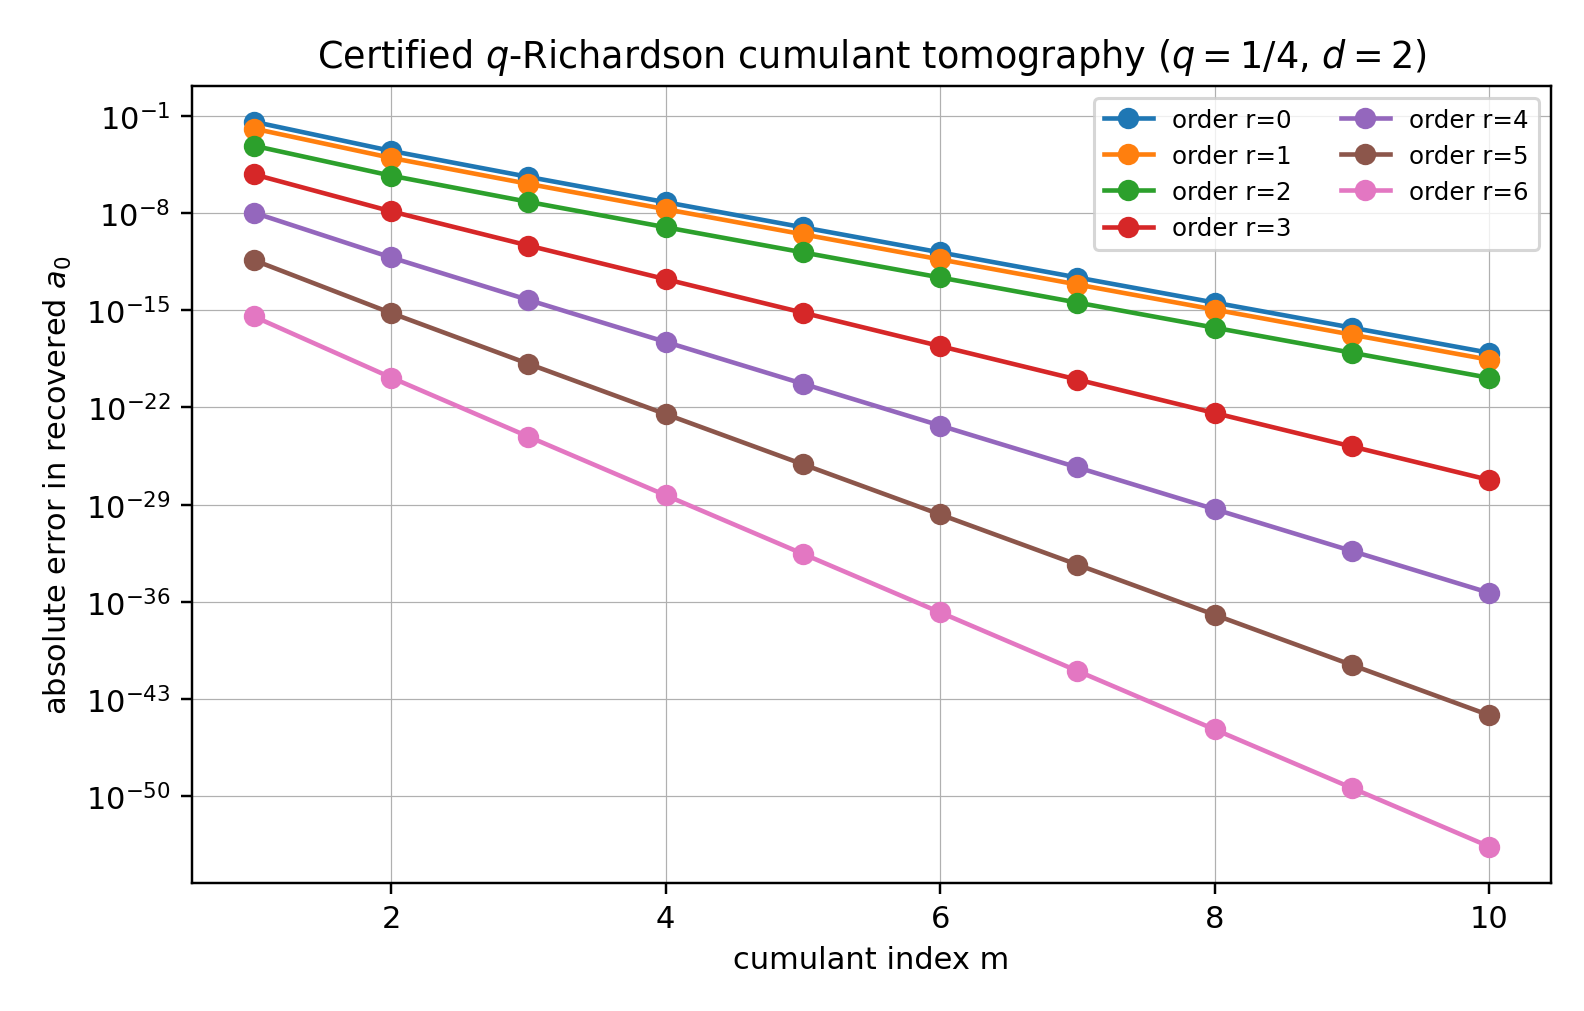
\includegraphics[width=0.91\textwidth]{assets/Fabius_Newton_Rvachev_Frontier_Report/figures/richardson_tomography.png}
\caption{Absolute errors in the recovery of $a_0$ from normalized cumulants
$A_2(4^{-m})$.  The CSV file retains the signs; the semilogarithmic plot shows the many
orders of magnitude gained by increasing either the cumulant index $m$ or the interpolation
order $r$.}
\label{p1:fig:richardson}
\end{figure}

The limiting interpolation condition number was recomputed as
\[
 1.96926035366826943194719369697\ldots,
\]
in agreement with \eqref{p1:eq:qquarter-condition}.  This is small enough that the observed
convergence reflects the exact tail annihilation rather than a cancellation between huge
floating-point weights.

\subsection{The sparse zero spectrum for $d=2$}

The generated file \path{zero_multiplicities_d2.csv} compares the prefix sum of the original
exponents with $1+\binom{\nu_2(n)}3$.  The first exceptional values are
\begin{center}
\begin{tabular}{@{}r r r@{}}
\toprule
$n$ & $\nu_2(n)$ & zero order\\
\midrule
$8$ & $3$ & $2$\\
$16$ & $4$ & $5$\\
$24$ & $3$ & $2$\\
$32$ & $5$ & $11$\\
$40$ & $3$ & $2$\\
$48$ & $4$ & $5$\\
$64$ & $6$ & $21$\\
\bottomrule
\end{tabular}
\end{center}
The spectrum is therefore classical at almost every integer but develops rapidly increasing
multiplicity on a sparse tower of highly divisible integers.

\subsection{Deterministic boundary-layer inversion}

For ranks $r=3,5,7,9$ (equivalently $d=2,4,6,8$), the script evaluates the exact truncated
characteristic product of $X_r$, inverts it on a nonaliasing FFT interval, normalizes the
resulting density, and compares its standardized CDF with the Gaussian.  The largest observed
CDF errors on $[-4,4]$ are shown in \cref{p1:tab:boundary-errors}.

\begin{table}[htbp]
\centering
\small
\caption{Deterministic FFT check of the standardized Pascal CDF.}
\label{p1:tab:boundary-errors}
\begin{tabular}{@{}r r r@{}}
\toprule
Rank $r$ & family degree $d=r-1$ & maximum CDF error on $[-4,4]$\\
\midrule
3 & 2 & $7.6043\times10^{-3}$\\
5 & 4 & $2.4624\times10^{-3}$\\
7 & 6 & $9.3598\times10^{-4}$\\
9 & 8 & $6.4752\times10^{-4}$\\
\bottomrule
\end{tabular}
\end{table}

\begin{figure}[htbp]
\centering
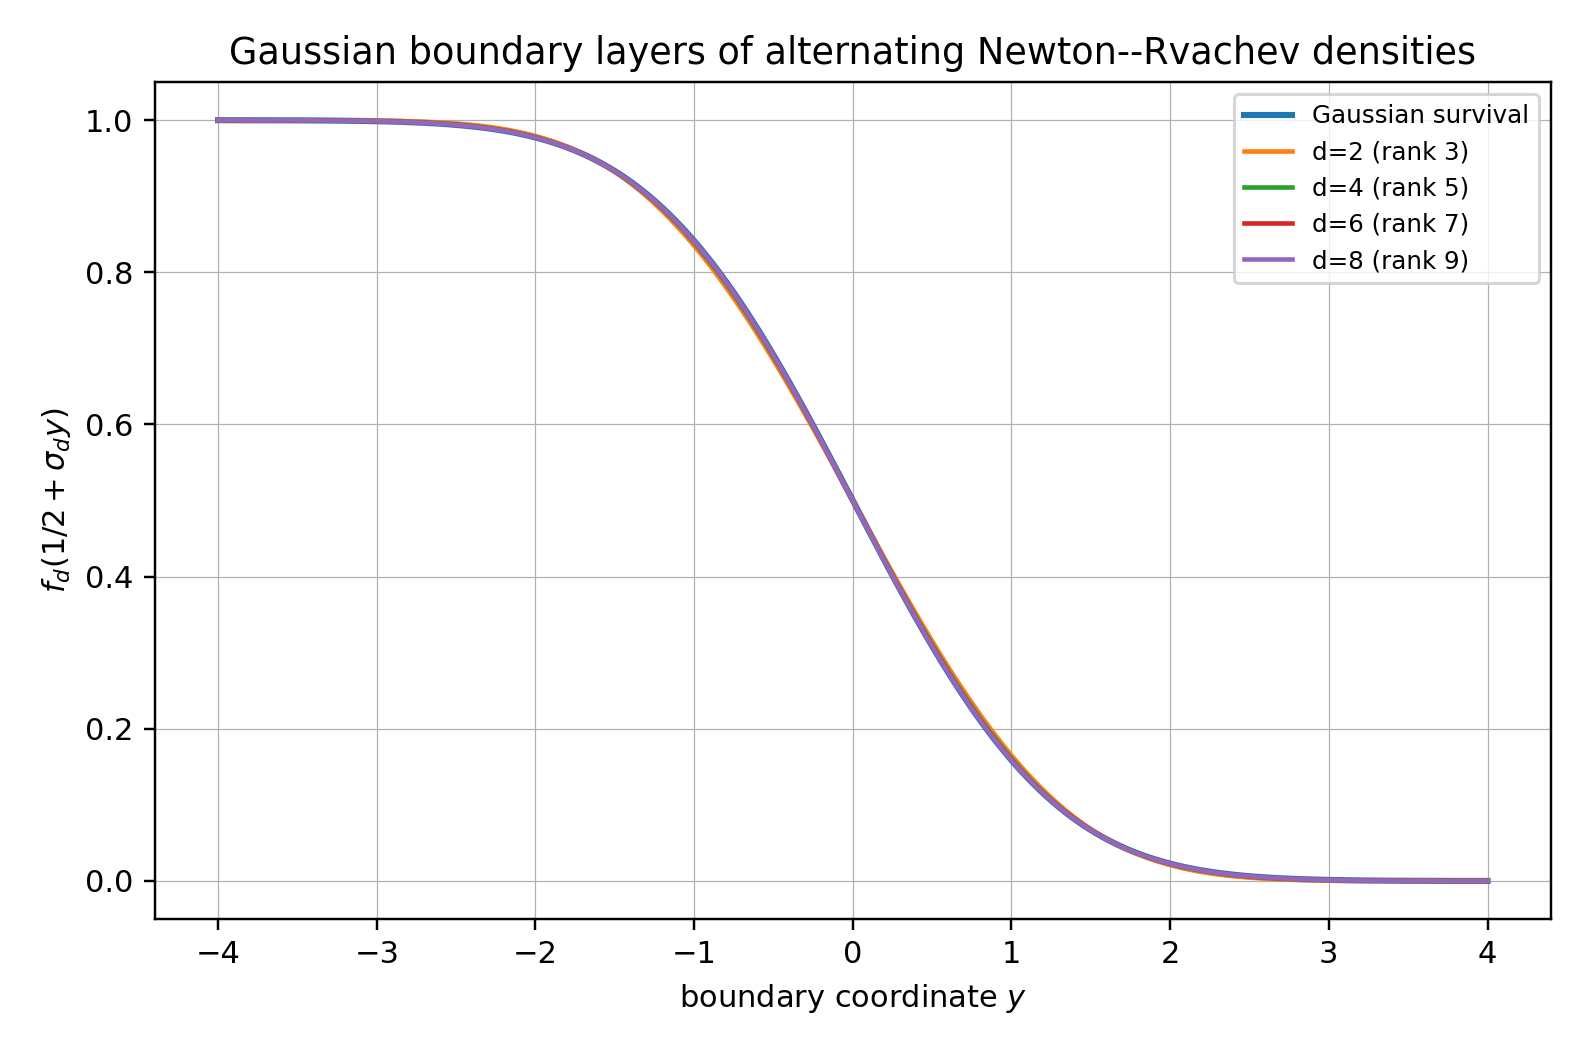
\includegraphics[width=0.91\textwidth]{assets/Fabius_Newton_Rvachev_Frontier_Report/figures/boundary_layers.png}
\caption{Right-edge boundary profiles
$f_d(1/2+\tau_dy)$ compared with the Gaussian survival function
$1-\NormalCDF(y)$.  The curves are obtained by deterministic Fourier inversion of the
Pascal--Rvachev characteristic products.}
\label{p1:fig:boundary-layers}
\end{figure}

The errors decrease consistently with \cref{p1:thm:pascal-BE}.  The theorem's universal
Berry--Esseen bound is intentionally conservative; the exact standardized fourth cumulant
\eqref{p1:eq:pascal-standardized-k4} gives a better explanation of the observed first
correction.

\subsection{Reproduction command}

From the extracted archive, the full experiment can be rerun with
\begin{lstlisting}[style=python]
python numerical_experiments.py --output-dir reproduced-data
\end{lstlisting}
The script checks its own exact identities with assertions before writing any figure.  A
failure therefore stops the run rather than silently producing visually plausible output.


\section{Conjectures and frontier problems}
\label{p1:sec:open}

The following statements are deliberately separated from the proved theorem package.  Each
is supported by the exact structure above, but each still requires a substantive analytic,
optimization, or arithmetic argument.

\begin{conjecture}[Uniform Edgeworth boundary expansion]
\label{p1:conj:edgeworth}
Let $r=d+1$ and $\tau_d$ be \eqref{p1:eq:tau-d}.  For every fixed $J$ and every fixed number of
$y$-derivatives, the two boundary profiles admit a uniform expansion
\begin{equation}
 f_d\!\left(\frac12+\tau_dy\right)
 =\NormalSurv(y)
  +\varphi(y)\sum_{j=1}^{J}E_j(y;r)
  +o\!\left((3/5)^{J(r+1)}\right),
 \label{p1:eq:edgeworth-conj}
\end{equation}
where $\varphi$ is the Gaussian density and each $E_j$ is an explicit Hermite polynomial
whose coefficients are Bell polynomials in the standardized cumulants.  The first correction
is governed by
$\kappa_4/\sigma^4=-2(3/5)^{r+1}$.
\end{conjecture}

\paragraph{Why it is plausible.}
The triangular array has bounded summands, an entire characteristic function, and
standardized cumulants that decay exponentially with rank.  A Fourier proof should be
considerably cleaner than a generic Edgeworth theorem because the exact product provides
uniform control in both the central and large-frequency regions.

\begin{conjecture}[Minimax property of alternating $q$-tomography]
\label{p1:conj:minimax}
Fix $q,m,r$ and the cone
\[
 \mathcal C_M=
 \left\{A(x)=\sum_{h\ge0}a_hx^h:a_h\ge0,
 \ A(q^m)\le M\right\}.
\]
Among all linear estimators using $A(q^m),\ldots,A(q^{m+r})$ and exact on polynomials of
degree at most $r$, the Lagrange estimator \eqref{p1:eq:Rrm-def} minimizes the worst one-sided
error on $\mathcal C_M$.  Moreover, consecutive odd/even transforms form the narrowest
possible universal bracket under these constraints.
\end{conjecture}

\paragraph{Why it is plausible.}
The remainder kernel in \eqref{p1:eq:Rrm-exact} has one sign on the coefficient cone and is the
unique kernel annihilating the first $r$ monomials.  That uniqueness is already formal:
\lean{Fabius.eq_lagrangeEvalWeight_of_moments} (\lean{GeometricLagrange.lean}) shows that on any
finite family of distinct field-valued nodes the Lagrange row is the only row with the
prescribed moments, with no nonzeroness or positivity assumption on the competing weights.  A
proof of the conjecture should be expressible as a finite-dimensional linear-programming
duality or a Chebyshev-system extremal argument.

\begin{conjecture}[Rational refinement transseries]
\label{p1:conj:rational-transseries}
Let $A$ be rational, nonnegative coefficientwise, and analytic at the origin.  Then the
complete large-$t$ transseries of $\log L_a(t)$ is determined functorially by the poles of
$A$: each pole $\rho$ of order $m$ produces vertical Mellin lattices
\[
 w=\frac{\log\rho+2\pi\ii k}{\log2},
 \qquad k\in\Z,
\]
with degree-$(m-1)$ logarithmic amplitudes.  Poles on the unit circle yield bounded
log-periodic phases; poles of other moduli yield additional power scales.  No further
frequencies occur.
\end{conjecture}

\paragraph{Research route.}
Start from \eqref{p1:eq:La-mellin}; establish a common meromorphic continuation and vertical
bounds for the rational factor, Gamma, and zeta; then shift the Mellin contour across a
finite set of pole lattices.  The main technical issue is uniform summability of the residue
series when several pole lattices have the same real part.

\begin{conjecture}[All-orders generalized inverse-Fabius expansion]
\label{p1:conj:inverse-transseries}
For every nonnegative integer-valued polynomial $P$ of degree $d$, the endpoint CDF $G_P$ and
its inverse admit all-orders expansions in the generalized lower-Lambert coordinate
\eqref{p1:eq:generalized-lambert}.  Their coefficients are finite differential polynomials in
the degree-$d$ periodic amplitudes of \eqref{p1:eq:logLP-structure}; equivalently, they are
algorithmically generated from N\"orlund Bernoulli polynomials, Gamma--zeta jets, and
complete Bell polynomials.  The expansion is uniform under bounded shifts of the Lambert
phase.
\end{conjecture}

\paragraph{Why it matters.}
This would extend the corpus's inverse Fabius theory from the rank-one quadratic logarithmic
saddle to every polynomial Newton sector and would make the Lambert--Bernoulli--Bell
connection exact rather than merely formal.

\begin{problem}[The Newton positivity cone]
\label{p1:prob:newton-cone}
Classify the integer vectors $(c_0,\ldots,c_d)$ for which
\[
 P(h)=\sum_{r=0}^{d}c_r\binom hr\ge0
 \qquad(h\in\N_0).
\]
Describe the extreme rays, the indecomposable characteristic functions
$\prod_r\Phi_{r+1}^{c_r}$, and the minimal Pascal numerator and denominator after all entire
cancellations.  Determine whether the alternating vectors
$((-1)^d,(-1)^{d-1},\ldots,1)$ for even $d$ generate distinguished extreme rays under a
natural support normalization.
\end{problem}

\begin{problem}[Arithmetic of generalized half-integer spectra]
For a rational generating function $A$ with integer coefficients, classify the fields,
traces, and norms of
\[
 \Phi_a\!\left(k+\frac12\right).
\]
The audited half-integer report handles the classical exponent sequence.  The master
zero/cumulant dictionary suggests that rational $A$ should produce finite-dimensional
cyclotomic trace recurrences, but the orders and positivity constraints will depend on the
pole data of $A$.
\end{problem}

\begin{problem}[Optimal smooth approximation of the box within the Newton family]
At fixed support and fixed highest Newton degree, choose a nonnegative integer-valued
polynomial $P$ to minimize one of
\[
 \|f_P-b\|_1,
 \qquad
 W_2(\Law(X_P),\Law(U)),
 \qquad
 \sup_{|\xi|\le T}|\Phi_P(\xi)-\sinc(\xi)|.
\]
The family $P_d(h)=\binom{h-1}{d}$ is natural because it appends one rescaled Pascal law to a
box, but it is not yet known to be extremal under any of these criteria.
\end{problem}


\section{Formalization and computational research program}
\label{p1:sec:formalization}

The theorem package is unusually suitable for staged Lean formalization: its algebraic core
is finite, and the analytic results can be added only after the exact identities are stable.
A dependency-aware order is as follows.

\subsection{Phase I: finite algebra and digital combinatorics}

\begin{enumerate}
\item Define exponent prefixes and prove
      $m_a(n)=\sum_{h\le\nu_2(n)}a_h$ for finite products.
\item Prove the finite zero-count identity
      $M_a(N)=\sum_ha_h\lfloor N/2^h\rfloor$ and the binary defect
      \eqref{p1:eq:M-bit}.
\item Define the generalized sign character and prove
      \eqref{p1:eq:kernel-shift}; formalize the automaticity equivalence for eventually
      periodic parity words.
\item Prove the finite sign-product factorization \eqref{p1:eq:T-a-L}, its exact order at one,
      and the first surviving moment \eqref{p1:eq:first-surviving}.
\item The geometric Lagrange weights, Gaussian-binomial closed form, exact
      principal specialization, survivor moments, finite residual sign, and exact finite
      norm are now formalized.  The exact transformed series is also formalized under
      unconditional summability in \path{AnalyticSeriesFilter.lean}, and
      \path{RvachevQBinomialFilter.lean} applies it to the actual infinite Rvachev
      sinc product.  The report's finite-prefix quotient and Bell series, positivity,
      sign-certified bounds, and uniform or asymptotic estimates remain open.
\end{enumerate}

These statements require only finite sums, polynomials, valuations, and existing
$q$-binomial infrastructure.  Several of them are in fact already discharged in the library, in
greater generality than is needed here: step~1 and the floor identity of step~2 by
\lean{Fabius.weightedScaleMultiplicity} and
\lean{Fabius.sum_range_weightedScaleMultiplicity}; the sharp moment of step~4 by
\lean{Fabius.sum_powerset_neg_one_pow_pow_card}, together with its vanishing companion
\lean{Fabius.sum_powerset_neg_one_pow_eval_of_degree_lt}; and the annihilation and first
surviving moment of step~5 by \lean{Fabius.sum_geometricLagrangeWeight_mul_pow} and
\lean{Fabius.sum_geometricLagrangeWeight_mul_pow_succ}, with
\lean{Fabius.geometricLagrange_richardson_exact} already giving module-valued Richardson
exactness.  What genuinely remains in Phase~I is the binary defect \eqref{p1:eq:M-bit}, the
automaticity equivalence of step~3, the sign-product factorization \eqref{p1:eq:T-a-L} and its
free-even-layer count, and the report-specific ordered sign and bound built on the now-formal
general-$q$ survivor.  The closed Gaussian-binomial form and every positive survivor moment
are no longer Phase~I obligations.

\subsection{Phase II: probability and entire products}

\begin{enumerate}
\item Construct $X_a$ from finite uniform sums and pass to the bounded infinite series using
      the summability hypothesis $A(1/2)<\infty$.
\item Prove local uniform convergence of $\Phi_a$ and the convolution-monoid law.
\item Derive cumulants from the uniform Bernoulli expansion and moments from the existing
      Bell-polynomial library.
\item Formalize identifiability first from zero multiplicities, then from analytic samples
      $A(4^{-j})$.
\item Build polynomial exponent sequences from Newton expansions and prove the entire
      cancellation behind \eqref{p1:eq:newton-Phi-factorization}.
\end{enumerate}

\subsection{Phase III: asymptotics and inverse functions}

\begin{enumerate}
\item Reuse the corpus's Mellin kernel theorem to prove \eqref{p1:eq:La-mellin} for polynomial
      weights.
\item Formalize pole orders and the leading coefficient $C_P$ before attempting the full
      periodic residue expansion.
\item Transfer the existing Pascal-hierarchy Fourier envelope to a general polynomial by
      the Newton factorization and lower-order comparison.
\item Prove the leading small-ball and inverse laws.  The library contains no de
      Bruijn--Voss exponential Tauberian transfer, so this step must begin by isolating that
      theorem as a reusable library component.
\item Only then lift the classical all-orders saddle and inverse-Lambert machinery to the
      higher-order pole hierarchy.
\end{enumerate}

\subsection{Certified computation}

The tomography algorithm is a natural application for exact rationals and interval
arithmetic.  At $q=1/4$ all Lagrange weights are rational, as are the normalized cumulants of
integer exponent sequences.  A verified executable can therefore recover coefficients with
no floating-point assumptions.  For asymptotic experiments, Arb-style ball arithmetic would
certify Mellin residues, Lambert branches, and boundary-layer errors.  The supplied Python
script is a reproducible exploratory implementation, not a substitute for that final
certification layer.


\section{Conclusion}
\label{p1:sec:conclusion}

The central result of this report is a change of viewpoint.  Instead of treating the
classical Rvachev transform, the Pascal hierarchy, its zero spectrum, its cumulants, and its
endpoint asymptotics as separate constructions, one begins with the exponent generating
function
\[
 A(q)=\sum_{h\ge0}a_hq^h.
\]
The same $A$ then appears at four geometrically related arguments:
\begin{equation}
 \begin{array}{ccl}
 A(1/2) &:& \text{twice the support radius},\\
 A(2^{-s}) &:& \text{spectral zeta and zero divisor},\\
 A(4^{-j}) &:& \text{even cumulants},\\
 A(2^w) &:& \text{endpoint Mellin transform}.
 \end{array}
 \label{p1:eq:four-samples-summary}
\end{equation}
Its coefficient parity is the Fourier-lobe character, its prefix sums are zero
multiplicities, its rationality is finite refinement rank, and its Newton coordinates are
Pascal--Rvachev exponents.

Three consequences seem especially durable.

First, the spectral and probabilistic data are identifiable: the zero divisor or the full
even-cumulant sequence determines the hidden dyadic convolution law.  The
Gaussian-$q$-binomial Richardson transform makes that statement constructive and supplies
certified alternating bounds.

Second, nonnegative integer-valued polynomials form a rich positive-definite quotient sector.
Negative Pascal exponents are not pathologies when they recombine into a nonnegative scale
sequence.  The family
$P_d(h)=\binom{h-1}{d}$ gives the explicit quotient
$\Phi_1\Phi_3/\Phi_2$ at $d=2$, sparse enhanced zero divisors, automatic lobe signs, and a
smooth approximation to the box with an exact Gaussian edge profile.

Third, Mellin reflection makes the endpoint and spectrum literally the same meromorphic
object viewed at $s$ and $-s$.  Polynomial degree becomes pole order; pole order becomes the
power of the endpoint logarithm; the dyadic pole lattice becomes the periodic coefficient
hierarchy; and the leading saddle is solved by a generalized lower branch of Lambert $W$.
N\"orlund Bernoulli polynomials and complete Bell polynomials then supply the coefficient
algebra required for an all-orders inverse theory.

These deductions are new relative to the pinned 67-source corpus, but they are not presented
as the end of the subject.  Their main value is that they turn a collection of striking
special identities into a classification problem with exact algebraic coordinates, stable
reconstruction algorithms, and a clear route to formal verification.

\appendix
\section{Complete recursive corpus inventory}
\label{p1:app:inventory}

The following path ledger is the authoritative source list used for the nonduplication audit.
Every path is relative to \path{Analysis/FabiusFunction/docs/}.  The pinned commit is
\texttt{32d6d36c51d803289e6d6a0dc0c37753766eba47}.  The count is 67.  Frozen revisions were
read for distinctive claims and provenance, but a repeated theorem in several revisions was
counted once when determining novelty.

{\small
\begin{longtable}{@{}r >{\raggedright\arraybackslash}p{0.88\textwidth}@{}}
\toprule
No. & Relative path\\
\midrule
\endfirsthead
\multicolumn{2}{c}{\small\itshape Corpus inventory (continued)}\\[0.3em]
\toprule
No. & Relative path\\
\midrule
\endhead
\midrule
\multicolumn{2}{r}{\small\itshape Continued on the next page}\\
\endfoot
\bottomrule
\endlastfoot
1 & \path{FabiusFunction_Mathematical_Glossary/FabiusFunction_Mathematical_Glossary.tex}\\
2 & \path{Fabius_Function_and_Rvachev_Up/Fabius_Function_and_Rvachev_Up.tex}\\
3 & \path{Non_Elementarity_of_the_Fabius_Function/Non_Elementarity_of_the_Fabius_Function.tex}\\
4 & \path{fabius_lean_walkthrough/fabius_lean_walkthrough.tex}\\
5 & \path{semi-formalized-research-frontiers/semi-formalized-research-frontiers.tex}\\
6 & \path{archive/early-notes/Fabius Asymptotic/Fabius Asymptotic.tex}\\
7 & \path{archive/early-notes/K-fold summation over the signed Thue-Morse sequence/K-fold summation over the signed Thue-Morse sequence.tex}\\
8 & \path{archive/glossary/FabiusFunction_Mathematical_Glossary-2/FabiusFunction_Mathematical_Glossary.tex}\\
9 & \path{archive/glossary/FabiusFunction_Mathematical_Glossary/FabiusFunction_Mathematical_Glossary.tex}\\
10 & \path{archive/lean-walkthrough/Fabius_Function_Lean_Walkthrough/Fabius_Function_Lean_Walkthrough.tex}\\
11 & \path{archive/lean-walkthrough/fabius_lean_walkthrough/fabius_lean_walkthrough.tex}\\
12 & \path{archive/primary-exposition/Fabius_Function_and_Rvachev_Up-2/Fabius_Function_and_Rvachev_Up.tex}\\
13 & \path{archive/primary-exposition/Fabius_Function_and_Rvachev_Up-3/Fabius_Function_and_Rvachev_Up.tex}\\
14 & \path{archive/primary-exposition/Fabius_Function_and_Rvachev_Up/Fabius_Function_and_Rvachev_Up.tex}\\
15 & \path{archive/primary-exposition/Fabius_and_Rvachev_Up-2/Fabius_and_Rvachev_Up.tex}\\
16 & \path{archive/primary-exposition/Fabius_and_Rvachev_up/Fabius_and_Rvachev_up.tex}\\
17 & \path{archive/primary-exposition/Fabius_function_and_up_function/Fabius_function_and_up_function.tex}\\
18 & \path{archive/primary-supplements/Fabius_Function_Missing_Parts-2/Fabius_Function_Missing_Parts.tex}\\
19 & \path{archive/primary-supplements/Fabius_Function_Missing_Parts/Fabius_Function_Missing_Parts.tex}\\
20 & \path{archive/q-calculus/Fabius_q_Special_Functions/Fabius_q_Special_Functions.tex}\\
21 & \path{archive/q-calculus/fabius-q-special-functions/fabius-q-special-functions.tex}\\
22 & \path{archive/research-frontiers/Fabius_Dyadic_Asymptotic_Bridge/Fabius_Dyadic_Asymptotic_Bridge.tex}\\
23 & \path{archive/research-frontiers/Fabius_Dyadic_Formulae_and_Alternative_Representations/Fabius_Dyadic_Formulae_and_Alternative_Representations.tex}\\
24 & \path{archive/research-frontiers/Fabius_Dyadic_Formulae_to_Asymptotics/Fabius_Dyadic_Formulae_to_Asymptotics.tex}\\
25 & \path{archive/research-frontiers/Fabius_Dyadic_q_Connections/Fabius_Dyadic_q_Connections.tex}\\
26 & \path{archive/research-frontiers/Fabius_Thue_Morse_Convergence_Rate/Fabius_Thue_Morse_Convergence_Rate.tex}\\
27 & \path{archive/research-frontiers/Fabius_Thue_Morse_Convergence_Rates/Fabius_Thue_Morse_Convergence_Rates.tex}\\
28 & \path{archive/research-frontiers/Primary_Exposition_Gap_Register/Primary_Exposition_Gap_Register.tex}\\
29 & \path{archive/research-frontiers/Repeated_Integration_and_Rvachev_Up/Repeated_Integration_and_Rvachev_Up.tex}\\
30 & \path{archive/research-frontiers/Rvachev_Up_from_Repeated_Integration/Rvachev_Up_from_Repeated_Integration.tex}\\
31 & \path{archive/research-frontiers/Thue_Morse_Formula_Atlas-1/Thue_Morse_Formula_Atlas.tex}\\
32 & \path{archive/research-frontiers/Thue_Morse_Formula_Atlas-2/Consolidated_Formula_Atlas_for_the_Thue_Morse_Sequence.tex}\\
33 & \path{archive/research-frontiers/Thue_Morse_Formula_Atlas-3/Thue_Morse_Formula_Atlas.tex}\\
34 & \path{archive/research-frontiers/non-formalized-research-frontiers/semi-formalized-research-frontiers.tex}\\
35 & \path{archive/standalone-studies/Non_Elementarity_of_the_Fabius_Function/Non_Elementarity_of_the_Fabius_Function.tex}\\
36 & \path{archive/standalone-studies/Small_Argument_Asymptotics/Small_Argument_Asymptotics.tex}\\
37 & \path{archive/standalone-studies/fabius-inverse-dyadic-closed-form/fabius-inverse-dyadic-closed-form.tex}\\
38 & \path{semi-formalized-research-frontiers/drafts/Fabius_Arithmetic_Rays_Frontier_Report/Fabius_Arithmetic_Rays_Frontier_Report.tex}\\
39 & \path{semi-formalized-research-frontiers/drafts/Fabius_Half_Integer_Spectral_Frontier_Report/Fabius_Half_Integer_Spectral_Frontier_Report.tex}\\
40 & \path{semi-formalized-research-frontiers/drafts/Fabius_Rvachev_Frontier_Report-2/Fabius_Rvachev_Frontier_Report.tex}\\
41 & \path{semi-formalized-research-frontiers/drafts/Fabius_Rvachev_Frontier_Report/Fabius_Rvachev_Frontier_Report.tex}\\
42 & \path{semi-formalized-research-frontiers/drafts/Fabius_Rvachev_New_Frontiers/Fabius_Rvachev_New_Frontiers.tex}\\
43 & \path{semi-formalized-research-frontiers/drafts/Fabius_Rvachev_Thue_Morse_Frontier_Results/Fabius_Rvachev_Thue_Morse_Frontier_Results.tex}\\
44 & \path{semi-formalized-research-frontiers/drafts/Spectral_Arithmetic_Pascal_Rvachev_Hierarchy/Spectral_Arithmetic_Pascal_Rvachev_Hierarchy.tex}\\
45 & \path{semi-formalized-research-frontiers/drafts/Thue_Morse_Formula_Atlas/Thue_Morse_Formula_Atlas.tex}\\
46 & \path{semi-formalized-research-frontiers/drafts/fabius_frontier_new_results/fabius_frontier_new_results.tex}\\
47 & \path{semi-formalized-research-frontiers/drafts/fabius_frontier_results_bundle/fabius_frontier_results.tex}\\
48 & \path{semi-formalized-research-frontiers/drafts/fabius_frontier_spectral_endpoint_report_bundle/fabius_frontier_spectral_endpoint_report.tex}\\
49 & \path{semi-formalized-research-frontiers/drafts/rvachev_up_fourier_decay/Rvachev_Up_Fourier_Decay-2/Rvachev_Up_Fourier_Decay.tex}\\
50 & \path{semi-formalized-research-frontiers/drafts/rvachev_up_fourier_decay/Rvachev_Up_Fourier_Decay-3/Fourier_decay_of_Rvachev_up.tex}\\
51 & \path{semi-formalized-research-frontiers/drafts/rvachev_up_fourier_decay/Rvachev_Up_Fourier_Decay_Comparative_Audit/Rvachev_Up_Fourier_Decay_Comparative_Audit.tex}\\
52 & \path{semi-formalized-research-frontiers/drafts/rvachev_up_fourier_decay/Rvachev_Up_Fourier_Decay_Gentle_Guide/Rvachev_Up_Fourier_Decay_Gentle_Guide.tex}\\
53 & \path{semi-formalized-research-frontiers/drafts/rvachev_up_fourier_decay/Rvachev_Up_Fourier_Decay_Second_Wave_Audit/Rvachev_Up_Fourier_Decay_Second_Wave_Audit.tex}\\
54 & \path{semi-formalized-research-frontiers/drafts/rvachev_up_fourier_decay/asymptotic-decay-rate-of-an-infinite-product-of-sinc-functions/asymptotic-decay-rate-of-an-infinite-product-of-sinc-functions.tex}\\
55 & \path{semi-formalized-research-frontiers/drafts/rvachev_up_fourier_decay/rvachev_up_fourier_decay-1/rvachev_up_fourier_decay.tex}\\
56 & \path{semi-formalized-research-frontiers/drafts/rvachev_up_fourier_decay/rvachev_up_fourier_decay-4/rvachev_up_fourier_decay.tex}\\
57 & \path{semi-formalized-research-frontiers/drafts/rvachev_up_fourier_decay/rvachev_up_fourier_decay-5/Rvachev_Up_Fourier_Decay_Final.tex}\\
58 & \path{semi-formalized-research-frontiers/drafts/rvachev_up_fourier_decay/rvachev_up_fourier_decay-6/Rvachev_Up_Fourier_Decay_Final_Synthesis.tex}\\
59 & \path{semi-formalized-research-frontiers/drafts/rvachev_up_fourier_decay/rvachev_up_fourier_decay-7/rvachev_up_fourier_decay_final.tex}\\
60 & \path{semi-formalized-research-frontiers/drafts/rvachev_up_fourier_decay/rvachev_up_fourier_decay-8/rvachev_up_fourier_decay_final.tex}\\
61 & \path{papers/AIF_2017__67_2_637_0/AIF_2017__67_2_637_0-corrected.tex}\\
62 & \path{papers/AIF_2017__67_2_637_0/AIF_2017__67_2_637_0.tex}\\
63 & \path{papers/arXiv-1502.06738v2/Lacunary_products.tex}\\
64 & \path{papers/arXiv-1702.05442v1/09-Function.tex}\\
65 & \path{papers/arXiv-1702.06487v3/157-Arithmetic-v3.tex}\\
66 & \path{papers/arXiv-2211.13570v1/document.tex}\\
67 & \path{papers/ubiq15/ubiq15-corrected.tex}\\
\end{longtable}
}


\section{Result ledger and dependency map}
\label{p1:app:ledger}

\Cref{p1:tab:result-ledger} records the logical status and principal inputs of the report's main
claims.  It is intended to make later formalization and peer checking easier: a reader can
separate finite algebra from analytic continuation, and new deductions from imported
frontier theorems.

\begin{longtable}{@{}>{\raggedright\arraybackslash}p{0.08\textwidth}>{\raggedright\arraybackslash}p{0.42\textwidth}>{\raggedright\arraybackslash}p{0.16\textwidth}>{\raggedright\arraybackslash}p{0.25\textwidth}@{}}
\caption{Result and proof-dependency ledger.}
\label{p1:tab:result-ledger}\\
\toprule
ID & Statement & Status & Main inputs\\
\midrule
\endfirsthead
\toprule
ID & Statement & Status & Main inputs\\
\midrule
\endhead
A1 & Exponent-sequence probability law, support, entire product, convolution monoid & proved & uniform characteristic function; normal convergence\\
A2 & Zero multiplicity $m_a(n)$ and zeta $\zeta(s)A(2^{-s})$ & proved & Euler product; Tonelli/rearrangement\\
A3 & Digital zero defect and generalized lobe character & proved & binary floors; parity\\
A4 & Automaticity iff the parity word is eventually periodic & proved & exact $2$-kernel/shift identity\\
A5 & General Prouhet order and first surviving power moment & proved & finite product; falling factorials\\
B1 & Cumulant transform $B_{2j}A(4^{-j})/(2j)$ & proved & uniform cumulants; additivity\\
B2 & Identifiability from zeros, zeta, or all even cumulants & proved & prefix differences; identity theorem\\
B3 & Gaussian-$q$-binomial tomography and one-sided remainder & proved & Lagrange interpolation; principal specialization\\
B4 & Bounded exact condition number $(-q;q)_r/(q;q)_r$ & proved & finite $q$-binomial theorem\\
C1 & Shift/refinement identity and rational finite-rank classification & proved & reindexing; rational-series theorem\\
C2 & Newton factorization of nonnegative polynomial weights & proved & integer-valued polynomial calculus\\
C3 & Leading Fourier, small-ball, and inverse laws & derived & audited Pascal hierarchy; de Bruijn transfer\\
D1 & Alternating family $P_d(h)=\binom{h-1}{d}$ and positive quotient & proved & Newton identity; random-series factorization\\
D2 & Sparse spectrum, exact cumulants, automatic Prouhet selector & proved & hockey-stick; Lucas theorem\\
D3 & Gaussian edge layer, exact $L^1$ law, TV and $W_2$ bounds & proved & Berry--Esseen; interval overlap\\
E1 & Mellin reflection between endpoint Laplace and spectral zeta & proved & Mellin kernel; geometric scaling\\
E2 & Polynomial/log-periodic pole hierarchy & proved structurally & Mellin residues; rational pole orders\\
E3 & All-orders generalized inverse transseries & conjectural & uniform higher-pole saddle analysis needed\\
\bottomrule
\end{longtable}

\paragraph{Lean crosswalk for B3--B4.}
The finite weight, all-moment, residual-sign, and finite-norm identities in
B3--B4 are formalized in \path{GeometricQBinomialLagrange.lean},
\path{GeometricLagrangeQBinomial.lean}, and
\path{GeometricLagrangeQMoments.lean}.  The exact unconditionally summable
transformed series, including the shifted Gaussian tail, is formalized in
\path{AnalyticSeriesFilter.lean}; zero-weight nodes require no convergence of
their unweighted samples.  The infinite condition-number limit on the whole range
\(0\le q<1\) is formalized in \path{LimitConditionNumber.lean} by
\lean{Fabius.tendsto\_sum\_abs\_qToeplitzWeight}, with left-limit divergence
at one proved by
\lean{Fabius.tendsto\_qConditionNumberLimit\_atTop\_at\_one\_left}.  The conditionally convergent
boundary, the ordered one-sided sign and bound, the report's finite-prefix
exponent/Bell generating function, and the uniform estimates remain results
of this report rather than claims about the current Lean corpus.  The distinct
actual infinite-product Rvachev instantiation is now formalized in
\path{RvachevQBinomialFilter.lean}.

\section{Reproducibility manifest}
\label{p1:app:manifest}

The companion archive contains:
\begin{center}
\begin{tabularx}{0.96\textwidth}{@{}p{0.34\textwidth}X@{}}
\toprule
Path & Purpose\\
\midrule
\path{Exponent_Sequence_Newton_Rvachev_Frontiers.tex} & Complete manuscript source.\\
\path{Exponent_Sequence_Newton_Rvachev_Frontiers.pdf} & Rendered report.\\
\path{numerical_experiments.py} & Commented high-precision and FFT verification program.\\
\path{figures/richardson_tomography.png} & Figure used in \cref{p1:fig:richardson}.\\
\path{figures/boundary_layers.png} & Figure used in \cref{p1:fig:boundary-layers}.\\
\path{data/richardson_tomography.csv} & Full signed extrapolation errors.\\
\path{data/boundary_layer_errors.csv} & Deterministic standardized-CDF errors.\\
\path{data/zero_multiplicities_d2.csv} & Direct and closed-form zero orders for the $d=2$ family.\\
\path{data/verification_log.txt} & Precision settings, assertion status, and headline values.\\
\path{README.md} & Build and reproduction commands.\\
\path{requirements.txt} & Exact Python package versions used for the numerical audit.\\
\path{SHA256SUMS} & Checksums for the report, code, figures, and data.\\
\bottomrule
\end{tabularx}
\end{center}

The numerical script fixes the precision and grid sizes explicitly.  Its formulas use
\texttt{numpy.sinc(x)}=$\sin(\pi x)/(\pi x)$, matching the normalization in
\eqref{p1:eq:sinc-normalized}.  The FFT interval is wider than the compact support, so periodic
copies do not overlap.  All exact checks run before figure generation.


\begin{thebibliography}{99}

\bibitem{p1:aistleitner2015}
C.~Aistleitner, R.~Hofer, and G.~Larcher,
\emph{On parametric Thue--Morse sequences and lacunary trigonometric products},
arXiv:1502.06738v2, 2015.

\bibitem{p1:alloucheShallit}
J.-P.~Allouche and J.~Shallit,
\emph{Automatic Sequences: Theory, Applications, Generalizations},
Cambridge University Press, 2003.

\bibitem{p1:andrews1976}
G.~E.~Andrews,
\emph{The Theory of Partitions},
Encyclopedia of Mathematics and its Applications, Vol.~2,
Addison--Wesley, 1976; reprinted by Cambridge University Press.

\bibitem{p1:arias1982}
J.~Arias de Reyna,
\emph{An infinitely differentiable function with compact support: definition and
properties}, Rev. Real Acad. Ciencias Madrid \textbf{76} (1982), 21--38;
English translation, arXiv:1702.05442, 2017.

\bibitem{p1:arias2017}
J.~Arias de Reyna,
\emph{Arithmetic of the Fabius function},
Ann. Inst. Fourier (Grenoble) \textbf{67} (2017), no.~2, 637--679;
arXiv:1702.06487v3.

\bibitem{p1:corless1996}
R.~M.~Corless, G.~H.~Gonnet, D.~E.~G.~Hare, D.~J.~Jeffrey, and D.~E.~Knuth,
\emph{On the Lambert $W$ function},
Adv. Comput. Math. \textbf{5} (1996), 329--359.

\bibitem{p1:debruijn1959}
N.~G.~de Bruijn,
\emph{Pairs of slowly oscillating functions occurring in asymptotic problems concerning
the Laplace transform},
Nieuw Arch. Wisk. (3) \textbf{7} (1959), 20--26.

\bibitem{p1:flajolet1995}
P.~Flajolet, X.~Gourdon, and P.~Dumas,
\emph{Mellin transforms and asymptotics: harmonic sums},
Theoret. Comput. Sci. \textbf{144} (1995), 3--58.

\bibitem{p1:norlund1924}
N.~E.~N\"orlund,
\emph{Vorlesungen \"uber Differenzenrechnung},
Grundlehren der mathematischen Wissenschaften, Vol.~13,
Springer, Berlin, 1924.

\bibitem{p1:petrov1995}
V.~V.~Petrov,
\emph{Limit Theorems of Probability Theory: Sequences of Independent Random Variables},
Oxford Studies in Probability, Vol.~4, Clarendon Press, Oxford, 1995.

\bibitem{p1:stanley1997}
R.~P.~Stanley,
\emph{Enumerative Combinatorics, Vol.~1}, second printing,
Cambridge Studies in Advanced Mathematics, Vol.~49,
Cambridge University Press, 1997.

\bibitem{p1:toth2022}
L.~T\'oth,
\emph{Linear combinations of Dirichlet series associated with the Thue--Morse sequence},
Integers \textbf{22} (2022), Paper A98; arXiv:2211.13570.

\bibitem{p1:voss2009}
J.~Voss,
\emph{Upper and lower bounds in exponential Tauberian theorems},
Tbilisi Math. J. \textbf{2} (2009), 41--50; arXiv:0908.0642.

\bibitem{p1:proveit}
V.~Reshetnikov,
\emph{ProveIt: formal and expository development of the Fabius function},
GitHub repository, pinned in this report at commit
\texttt{32d6d36c51d803289e6d6a0dc0c37753766eba47}, 27 August 2026.

\end{thebibliography}


% extra macros for part 2
\newcommand{\up}{\operatorname{up}}
\newcommand{\ePartx}{\mathrm{e}}
\newcommand{\iiPartx}{\mathrm{i}}
\newcommand{\RPartx}{\mathbb{R}}
\newcommand{\CPartx}{\mathbb{C}}
\newcommand{\NPartx}{\mathbb{N}}
\newcommand{\D}{\mathrm{D}}
\newcommand{\norm}[1]{\left\lVert #1\right\rVert}
\newcommand{\abs}[1]{\left\lvert #1\right\rvert}
\newcommand{\qbinomPartx}[2]{\genfrac{[}{]}{0pt}{}{#1}{#2}_{q}}

% ed.: restore arabic section numbering after Part I's appendices
% (the consolidated volume let \appendix lettering run across the
% part boundary: Part II rendered as sections G--N with its own
% appendices restarting at A)
\setcounter{section}{0}
\renewcommand{\thesection}{\arabic{section}}
\part{q-Binomial Richardson Acceleration of Geometric Sinc Products}
% Absorbed from fabius_frontier_results/q_richardson_sinc_frontier.tex




\begin{abstract}
The Fourier transform of Rvachev's compactly supported up-function is the geometric
sinc product
\[
   P(\xi)=\prod_{\nu\geq 1}\sinc(\xi/2^\nu).
\]
The repository corpus develops its large-frequency decay, its connection with the
Fabius function and the signed Thue--Morse sequence, dyadic exact values,
small-argument and inverse asymptotics, and several Richardson-type limits.
This report studies a different asymptotic variable: the truncation level in the
finite product
\(P_n(\xi)=\prod_{\nu=1}^n\sinc(\xi/2^\nu)\).

For a general geometric base \(b>1\), with \(q=b^{-2}\), we prove, in the
disc \(\lvert q^n\xi^2\rvert<\pi^2b^2\), the total exact analytic factorization
\[
 P_{b,n}(\xi)
 =P_b(\xi)\exp\!\left(\sum_{k\geq1}c_k(b)\,\xi^{2k}q^{kn}\right)
 =P_b(\xi)\sum_{r\geq0}\alpha_r(b)\,\xi^{2r}q^{rn}.
\]
Off the zero set of \(P_b\), division gives the corresponding quotient form.
The cumulants \(c_k(b)\) are explicit Bernoulli-number combinations and the
coefficients \(\alpha_r(b)\) are complete Bell polynomials. Lagrange evaluation
at the geometric nodes \(1,q,\ldots,q^m\) then gives a universal extrapolant
\[
 \mathcal R_{m,n}P_b=\sum_{j=0}^m w_j^{(m)}P_{b,n+j},
 \qquad
 w_j^{(m)}=\frac{(-1)^{m-j}q^{(m-j)(m-j+1)/2}}
 {(q;q)_j(q;q)_{m-j}}.
\]
On the same disc and off the zero set of \(P_b\), its complete error series has
the closed q-binomial form
\[
 \frac{\mathcal R_{m,n}P_b(\xi)}{P_b(\xi)}-1
 =(-1)^m q^{\binom{m+1}{2}}
 \sum_{r\geq m+1}\qbinomPartx{r-1}{m}\alpha_r(b)\xi^{2r}q^{rn}.
\]
Consequences include an exact sign law, non-asymptotic divided-difference bounds,
a rigorous a posteriori error certificate, and a uniformly bounded stability
constant \(\prod_{r=1}^m(1+q^r)/(1-q^r)\). For \(q=1/4\) this constant stays
below \(1.970\), even as the order tends to infinity.

After inverse Fourier transformation, the same filter combines consecutive finite
box splines. It matches the first \(2m\) moments of the limiting up-density
\emph{exactly at every truncation level}, and converges in every \(C^s\)-norm at
rate \(q^{(m+1)n}\). The first error profile is an explicit even derivative of
the up-function. Translating to the Fabius function gives the same accelerated
approximation, while inversion on compact interior intervals yields an explicit
first correction for the inverse Fabius function. These statements are proved
here and checked symbolically and numerically by the accompanying Python program.
They are described as \emph{repository-new}: the claim is that they do not occur
in the audited \texttt{*.tex} corpus under the stated repository path, not that a
priority search over the entire literature has been completed.
\end{abstract}

\medskip
\noindent\textbf{Status of results.}
Every result labelled theorem, proposition, lemma, or corollary below has a proof
in this report. The numerical tables are reproducible from
\path{verify_frontier_results.py}.  The denominator-free finite
\(q\)-binomial theorem is formalized in \path{FiniteQBinomialCore.lean}, while
\path{GeometricLagrange.lean} proves mass one, cancellation of the first
geometric modes, the first surviving moment, and module-valued Richardson
exactness.  The already compiled \path{GeometricQBinomialLagrange.lean}
identifies the individual weights with their Gaussian-binomial quotients under
injectivity of the finite geometric node set.  At post-snapshot source
checkpoint \path{1e761ed77583e9870ceeaeb2c74ac824094f0f3f},
\path{GeometricCompleteHomogeneous.lean} and
\path{GeometricResidualMoments.lean} additionally formalize the
denominator-free principal specialization and the complete positive-degree
Gaussian \(q\)-moment formula, including common scales and shifted blocks.
At the reconciled source checkpoint
\path{f77ff7c296b99050107948f5aa2a9488aec01d05},
the rational layer is implemented in
\begin{center}
\path{GeometricQBinomialLagrange.lean}\\
\path{GeometricRichardson.lean}\\
\path{GeometricLagrangeWeights.lean}\\
\path{GeometricLagrangeQBinomial.lean}\\
\path{GeometricLagrangeQMoments.lean}.
\end{center}
These modules prove the finite rational
\(0<q<1\) weight formulas, the \(W_m(q^r)\) and \(q\)-Pochhammer moment
presentations, all residual moments and their sign, and the exact finite
\(\ell^1\) norm, including dedicated \(q=1/4\) corollaries.  The
generic transformed-error series is now formalized in
\path{AnalyticSeriesFilter.lean} under unconditional summability, with
nonzero-weight hypotheses only at samples that actually contribute.

The infinite condition-number limit is formalized too, in
\path{LimitConditionNumber.lean}, which lets $n$ grow in the closed form
$\sum_{j\le n}\lvert w_q(n,j)\rvert=(-q;q)_n/(q;q)_n$ of
\path{GeneralQConditionNumber.lean}: both families are multipliable, the finite
symbols converge to $(a;q)_\infty$, and the condition numbers converge to
$(-q;q)_\infty/(q;q)_\infty$
(\lean{Fabius.tendsto\_sum\_abs\_qToeplitzWeight}) on the whole range
$0\le q<1$.  The crux is positivity of the denominator, and it is worth
recording how it is obtained, because the obvious route fails: the one-shot
Weierstrass product bound has deficit budget $q/(1-q)$, which already reaches
$1$ at $q=\tfrac12$, and its vacuity at $q=\tfrac34$ is recorded as a theorem
rather than as prose (\lean{Fabius.weierstrass\_bound\_vacuous\_at\_three\_quarters}).
Positivity instead comes from summability of the logarithms, which needs no
threshold at all (\lean{Fabius.qPochhammerInf\_pos}).  The limit is bounded below
by $1$, attained exactly at $q=0$, and by $1/(1-q)$
(\lean{Fabius.one\_div\_one\_sub\_le\_qConditionNumberLimit}); it tends to
$+\infty$ as $q\uparrow1$
(\lean{Fabius.tendsto\_qConditionNumberLimit\_atTop\_at\_one\_left}), and at
$q=999/1000$ is already at least $1000$.

The named even-moment coefficients and their Gaussian filter for the actual
infinite Rvachev sinc product are now formalized.  Identifying instead the
report's finite-prefix quotient \(P_{b,n}/P_b\) with its Bell series, and
proving the resulting analytic signs, remainder and bracketing bounds,
uniform spline limits, asymptotics, and inverse-function consequences, remain
unformalized.



\section{Audit scope and the non-duplication boundary}

\subsection{How the corpus was used}

The source audit covered every LaTeX family in the repository documentation tree
\cite{p2:repo}, including the current expository volumes, the formalization walkthrough, the
non-elementarity article, the mathematical glossary, the consolidated frontier
volume, the Thue--Morse formula atlas, all waves of the Fourier-decay discussion,
the paper-source subdirectories, and the historical archive. The archive index
was used to track renamed and byte-identical historical variants, so that an old
statement was not mistaken for a new one merely because it appeared under a
superseded filename. A source map is given in \cref{p2:app:corpus}.

The audit revealed four especially important boundaries.

\begin{enumerate}[label=\textbf{B\arabic*.},leftmargin=12mm]
\item The main exposition and its supplements already contain the normalized
infinite sinc product, the box-convolution construction of \(\up\), its relation
to the Fabius function, dyadic identities, q-Pochhammer and q-binomial formulae,
and the signed Thue--Morse derivative comb.

\item The asymptotic documents already contain a corrected Lambert--\(W\)
endpoint scale, a periodic dyadic phase, and all-order small-argument expansions
for the Fabius function and its inverse. Those results concern
\(x\downarrow0\), not finite-product truncation \(n\to\infty\).

\item The Fourier-decay waves study \(\abs{P(\xi)}\) as
\(\abs{\xi}\to\infty\), including dyadic oscillation and exceptional
frequencies. They do not develop the exact analytic expansion of
\(P_{b,n}/P_b\) in the small geometric variable \(q^n\), nor the extrapolation
filter derived below.

\item The frontier volume already has q-Richardson ideas for discrete Fabius
spline rows and degree-dependent approximants. We therefore do not present a
generic Richardson recipe as new. The new object here is the \emph{Fourier-tail
truncation sequence} \(P_{b,n}\), for which the error coefficients, all q-moments,
stability constant, moment matching, and inverse-function consequence can all be
written exactly.
\end{enumerate}

The external search performed for this report also found general literature on
Richardson extrapolation and on powers of sinc expressed through Bell
polynomials, but no source matching the combined construction in
\cref{p2:sec:tail,p2:sec:filter,p2:sec:physical}. This is supporting evidence only, not an
exhaustive priority claim.

\subsection{What is new in this report}

The principal contributions are the following.

\begin{enumerate}[label=\textbf{N\arabic*.},leftmargin=12mm]
\item A one-variable analytic tail function \(\Phi_b\) whose Taylor cumulants
are rational Bernoulli combinations and whose Taylor coefficients are complete
Bell polynomials.

\item A q-Lagrange operator
\(W_m(T_q)=\prod_{r=1}^m(T_q-q^r)/(1-q^r)\) that annihilates the first \(m\)
truncation modes exactly.

\item An all-order q-binomial error identity, not merely a leading-order
Richardson estimate.

\item A closed stability constant with a finite infinite-order limit, and a
successive-level error certificate requiring no knowledge of the infinite
product.

\item Exact matching of the first \(2m\) moments of the limiting Rvachev density
by a signed combination of finite box splines, for every \(n\).

\item A \(C^\infty\) superconvergence theorem with an explicit first derivative
profile, followed by an interior inverse-Fabius perturbation formula.

\item A kernel-independent extension showing that the same q-filter accelerates
any geometric product whose elementary factor has an even logarithmic Taylor
series.
\end{enumerate}

\section{Geometric sinc products and finite Rvachev splines}
\label{p2:sec:setup}

Fix \(b>1\) and set
\[
 q=b^{-2}\in(0,1),\qquad \sinc z=\begin{cases}\sin z/z,&z\ne0,\\1,&z=0.\end{cases}
\]
Define
\begin{equation}
 P_b(\xi)=\prod_{\nu=1}^{\infty}\sinc(\xi/b^\nu),
 \qquad
 P_{b,n}(\xi)=\prod_{\nu=1}^{n}\sinc(\xi/b^\nu).
 \label{p2:eq:products}
\end{equation}
The convergence is locally uniform in \(\CPartx\), since
\(1-\sinc(\xi/b^\nu)=O(b^{-2\nu})\) on compact sets.

Let
\begin{equation}
 h_{b,\nu}(x)=\frac{b^\nu}{2}\,\mathbf 1_{[-b^{-\nu},b^{-\nu}]}(x),
 \qquad
 u_{b,n}=h_{b,1}*\cdots*h_{b,n}.
 \label{p2:eq:boxes}
\end{equation}
With the Fourier convention
\[
 \widehat f(\xi)=\int_{\RPartx}f(x)\ePartx^{-\iiPartx\xi x}\,dx,
 \qquad
 f(x)=\frac1{2\pi}\int_{\RPartx}\widehat f(\xi)\ePartx^{\iiPartx\xi x}\,d\xi,
\]
we have \(\widehat h_{b,\nu}(\xi)=\sinc(\xi/b^\nu)\), hence
\begin{equation}
 \widehat{u_{b,n}}=P_{b,n}.
 \label{p2:eq:finiteFT}
\end{equation}
The infinite convolution \(u_b=*_{\nu\geq1}h_{b,\nu}\) is a probability density
supported on \([-1/(b-1),1/(b-1)]\), and \(\widehat u_b=P_b\). The product
decays faster than every power, so \(u_b\in C_c^\infty(\RPartx)\). At \(b=2\),
\(u_2\) is the normalized Rvachev up-function.

\subsection{The finite Thue--Morse derivative comb}

The bridge to the signed Thue--Morse sequence is already part of the repository
background, but the exact normalization is useful for what follows. Write
\(t_k=(-1)^{s_2(k)}\), where \(s_2(k)\) is the binary digit sum.

\begin{proposition}[distributional Thue--Morse comb]
For \(n\geq1\),
\begin{equation}
 \D^n u_{2,n}
 =2^{n(n-1)/2}\sum_{k=0}^{2^n-1}t_k\,
 \delta_{-1+(2k+1)2^{-n}}.
 \label{p2:eq:TMcomb}
\end{equation}
\end{proposition}

\begin{proof}
For \(a>0\),
\[
 \D\left(\frac1{2a}\mathbf1_{[-a,a]}\right)
 =\frac1{2a}(\delta_{-a}-\delta_a).
\]
Differentiate every factor in \eqref{p2:eq:boxes}. Choosing the right endpoint in
the \(j\)-th factor contributes one minus sign. If the choices are encoded by
the binary digits of \(k\), the coefficient is \((-1)^{s_2(k)}\), while the
location is
\[
 -\sum_{j=1}^n2^{-j}+2\sum_{j=1}^n\varepsilon_j2^{-j}
 =-1+2^{-n}+(2^{1-n})k.
\]
Finally \(\prod_{j=1}^n(2\cdot2^{-j})^{-1}=2^{n(n-1)/2}\).
\end{proof}

Thus every finite product in \eqref{p2:eq:products} is simultaneously a Fourier
approximation and an integrated Thue--Morse object. The acceleration below acts
on both descriptions at once.

\section{The exact Bernoulli--Bell tail expansion}
\label{p2:sec:tail}

\subsection{A universal tail function}

The key observation is that the two variables \(n\) and \(\xi\) enter the omitted
tail only through \(q^n\xi^2\).

\begin{definition}
For \(z\) near zero, define
\begin{equation}
 \Phi_b(z)=\prod_{\ell=1}^{\infty}
 \frac1{\sinc(b^{-\ell}\sqrt z)}.
 \label{p2:eq:PhiDef}
\end{equation}
The expression is independent of the sign of \(\sqrt z\), and hence defines an
ordinary analytic function of \(z\).
\end{definition}

\begin{theorem}[exact tail factorization]
\label{p2:thm:tailfactor}
The function \(\Phi_b\) is analytic in \(\abs z<\pi^2b^2\), meromorphic in
\(\CPartx\), and has its nearest singularity to the origin at \(z=\pi^2b^2\). For
every \(n\geq0\),
\begin{equation}
 P_{b,n}(\xi)=P_b(\xi)\Phi_b(q^n\xi^2).
 \label{p2:eq:exacttail}
\end{equation}
The identity is entire in \(\xi\); at common zeros it is interpreted by analytic
continuation. Moreover,
\begin{equation}
 \Phi_b(z)=\frac{\Phi_b(qz)}{\sinc(b^{-1}\sqrt z)}.
 \label{p2:eq:PhiFunctional}
\end{equation}
\end{theorem}

\begin{proof}
Cancel the first \(n\) factors in \(P_b/P_{b,n}\) and write \(\nu=n+\ell\):
\[
 \frac{P_{b,n}(\xi)}{P_b(\xi)}
 =\prod_{\ell=1}^{\infty}
 \frac1{\sinc(\xi/b^{n+\ell})}
 =\Phi_b(q^n\xi^2).
\]
The zeros of \(\sinc(b^{-\ell}\sqrt z)\) occur at
\(z=\pi^2k^2b^{2\ell}\), \(k\in\mathbb Z\setminus\{0\}\). The nearest is
\(\pi^2b^2\). Splitting off the \(\ell=1\) factor and reindexing proves
\eqref{p2:eq:PhiFunctional}.
\end{proof}

\subsection{Bernoulli cumulants}

The classical expansion
\begin{equation}
 \log\sinc w=-\sum_{k=1}^{\infty}
 \frac{\zeta(2k)}{k\pi^{2k}}w^{2k},\qquad \abs w<\pi,
 \label{p2:eq:logsinc}
\end{equation}
turns the geometric tail into an explicitly summable cumulant series.

The analytic input in \eqref{p2:eq:logsinc} is already machine checked.
On the complex disk, \path{SincZetaSeries.lean} proves the branch-free
exponential forms \lean{Fabius.complexSinc\_pi\_mul\_eq\_cexp} and
\lean{Fabius.complexSinc\_eq\_cexp}; its real theorem
\lean{Fabius.log\_sin\_div\_pi\_mul} recovers the displayed logarithm
literally.  At the dyadic base, \path{SincZetaDyadic.lean} resums all
geometric scales in \lean{Fabius.rvachevFourierProduct\_eq\_cexp} and
\lean{Fabius.rvachevFourierProduct\_eq\_prefix\_mul\_cexp}, while
\path{SincZetaRemainder.lean} supplies the certified remaining zeta tail.
What is not yet packaged for this part is the general-\(b\) reciprocal-tail
coefficient sequence \(\alpha_r(b)\) and its concrete connection to the
geometric analytic filter below.

\begin{theorem}[Bernoulli cumulants]
\label{p2:thm:cumulants}
For \(\abs z<\pi^2b^2\),
\begin{equation}
 \Phi_b(z)=\exp\!\left(\sum_{k=1}^{\infty}c_k(b)z^k\right),
 \label{p2:eq:PhiCumulant}
\end{equation}
where
\begin{align}
 c_k(b)
 &=\frac{\zeta(2k)}{k\pi^{2k}(b^{2k}-1)}
 \label{p2:eq:ckzeta}\\
 &=\frac{(-1)^{k+1}2^{2k-1}B_{2k}}
 {k(2k)!(b^{2k}-1)}.
 \label{p2:eq:ckBernoulli}
\end{align}
In particular \(c_k(b)>0\) for every \(k\geq1\).
\end{theorem}

\begin{proof}
Insert \eqref{p2:eq:logsinc} into \eqref{p2:eq:PhiDef}, interchange absolutely
convergent sums, and use
\[
 \sum_{\ell=1}^{\infty}b^{-2k\ell}=\frac1{b^{2k}-1}.
\]
The Bernoulli form follows from Euler's formula for \(\zeta(2k)\). Positivity is
clear from \eqref{p2:eq:ckzeta}.
\end{proof}

Combining \cref{p2:thm:tailfactor,p2:thm:cumulants} gives the exact truncation expansion
\begin{equation}
 \frac{P_{b,n}(\xi)}{P_b(\xi)}
 =\exp\!\left(\sum_{k\geq1}c_k(b)\xi^{2k}q^{kn}\right).
 \label{p2:eq:tailn}
\end{equation}
This is an equality, not a merely formal asymptotic series, whenever
\(\abs\xi<\pi b^{n+1}\).

\subsection{Bell coefficients and their recurrence}

Write
\begin{equation}
 \Phi_b(z)=\sum_{r=0}^{\infty}\alpha_r(b)z^r,
 \qquad \alpha_0(b)=1.
 \label{p2:eq:alphadef}
\end{equation}

\begin{proposition}[complete Bell-polynomial formula]
\label{p2:prop:Bell}
Let \(Y_r\) denote the complete exponential Bell polynomial. Then
\begin{equation}
 \alpha_r(b)=\frac1{r!}
 Y_r\bigl(1!c_1(b),2!c_2(b),\ldots,r!c_r(b)\bigr),
 \label{p2:eq:Bellalpha}
\end{equation}
and equivalently
\begin{equation}
 r\alpha_r(b)=\sum_{k=1}^r k c_k(b)\alpha_{r-k}(b).
 \label{p2:eq:alpharec}
\end{equation}
Every \(\alpha_r(b)\) is strictly positive.
\end{proposition}

\begin{proof}
Equation \eqref{p2:eq:Bellalpha} is the defining exponential generating identity for
complete Bell polynomials. Differentiating \eqref{p2:eq:PhiCumulant} and comparing
coefficients gives \eqref{p2:eq:alpharec}. Positivity follows inductively from
\(c_k(b)>0\).
\end{proof}

For the Rvachev base \(b=2\), the first cumulants are
\begin{align*}
 c_1&=\frac1{18},&c_2&=\frac1{2700},&c_3&=\frac1{178605},\\
 c_4&=\frac1{9639000},&c_5&=\frac1{478533825},&
 c_6&=\frac{691}{15688261338750}.
\end{align*}
The corresponding Bell coefficients are
\begin{align}
 \alpha_0&=1,&
 \alpha_1&=\frac1{18},&
 \alpha_2&=\frac{31}{16200},\\
 \alpha_3&=\frac{2347}{42865200},&
 \alpha_4&=\frac{1904369}{1311675120000},&
 \alpha_5&=\frac{3309760579}{88561680752160000}.
 \label{p2:eq:alphaB2}
\end{align}
The exact rationals are useful because no numerical fitting is needed at any
order.

\section{q-Lagrange Richardson extrapolation}
\label{p2:sec:filter}

\subsection{The filter polynomial}

Let \(T_q\) be the dilation operator \((T_qf)(z)=f(qz)\). Define
\begin{equation}
 W_m(t)=\prod_{r=1}^m\frac{t-q^r}{1-q^r},
 \qquad W_0(t)=1.
 \label{p2:eq:Wm}
\end{equation}
Thus \(W_m(1)=1\) and \(W_m(q^r)=0\) for \(1\leq r\leq m\).
Expanding \(W_m(t)=\sum_{j=0}^m w_j^{(m)}t^j\) gives the following exact
weights.

\begin{theorem}[geometric Lagrange weights]
\label{p2:thm:weights}
For \(0\leq j\leq m\),
\begin{equation}
 w_j^{(m)}
 =\prod_{\substack{0\leq\ell\leq m\\\ell\ne j}}
 \frac{-q^\ell}{q^j-q^\ell}
 =\frac{(-1)^{m-j}q^{(m-j)(m-j+1)/2}}
 {(q;q)_j(q;q)_{m-j}},
 \label{p2:eq:weights}
\end{equation}
where \((q;q)_r=\prod_{s=1}^r(1-q^s)\). These are precisely the Lagrange
weights that recover the value at zero from data at \(1,q,\ldots,q^m\).
\end{theorem}

\begin{proof}
The first expression is the Lagrange cardinal basis evaluated at zero. Separating
factors with \(\ell<j\) and \(\ell>j\), then collecting powers of \(q\), gives the
second expression. Alternatively, the q-binomial theorem expands
\eqref{p2:eq:Wm} directly.
\end{proof}

\paragraph{Lean boundary for the individual weights.}
The source-level closed quotient predates the new all-residual tranche.  Over a field, under
\(
 \operatorname{InjOn}(j\mapsto q^j,\{0,\ldots,m\}),
\)
the declaration
\begin{center}
\path{geometricLagrangeWeight_eq_gaussianBinomial_div}
\end{center}
in \path{GeometricQBinomialLagrange.lean} gives the numerator with the deliberate
reverse index \path{gaussianBinomial q m (m - j)}.  The displayed symmetric-
index notation in \eqref{p2:eq:weights} is the equivalent paper convention, not a
claim that this checkpoint added a generic Gaussian-symmetry theorem.
\begin{samepage}
The same module also contains the following cleared-denominator identity:
\begin{center}
\path{finiteQPochhammerIn_mul_geometricLagrangeWeight_eq}.
\end{center}
\end{samepage}
In the present
real range \(0<q<1\), the required finite-node injectivity is automatic.  These
pointwise weight results should not be attributed to the later
principal-specialization module.

\begin{definition}[accelerated finite product]
For \(m,n\geq0\), define
\begin{equation}
 \mathcal R_{m,n}P_b(\xi)
 =\sum_{j=0}^m w_j^{(m)}P_{b,n+j}(\xi).
 \label{p2:eq:Rdef}
\end{equation}
\end{definition}

With \(z=q^n\xi^2\), the tail factorization gives the compact operator identity
\begin{equation}
 \frac{\mathcal R_{m,n}P_b(\xi)}{P_b(\xi)}
 =\bigl(W_m(T_q)\Phi_b\bigr)(z).
 \label{p2:eq:operatoridentity}
\end{equation}
The right side is well defined as an analytic continuation even at common zeros.

\subsection{A Romberg-style triangular algorithm}

The factorization of \(W_m\) gives a recursion that avoids an explicit weighted
sum.

\begin{algorithm}[q-Richardson table]
\label{p2:alg:table}
Start with \(A_{0,n}=P_{b,n}(\xi)\). For \(m\geq1\), form
\begin{equation}
 A_{m,n}=\frac{A_{m-1,n+1}-q^mA_{m-1,n}}{1-q^m}.
 \label{p2:eq:table}
\end{equation}
Then \(A_{m,n}=\mathcal R_{m,n}P_b(\xi)\).
\end{algorithm}

\begin{proof}
The polynomial recursion
\[
 W_m(t)=\frac{t-q^m}{1-q^m}W_{m-1}(t)
\]
becomes \eqref{p2:eq:table} after applying it to the shift \(n\mapsto n+1\).
\end{proof}

For \(b=2\), \(q=1/4\), the first filters are
\begin{align}
 \mathcal R_{1,n}P&=\frac{4P_{n+1}-P_n}{3},
 \label{p2:eq:m1}\\
 \mathcal R_{2,n}P&=\frac{P_n-20P_{n+1}+64P_{n+2}}{45},
 \label{p2:eq:m2}\\
 \mathcal R_{3,n}P&=\frac{-P_n+84P_{n+1}-1344P_{n+2}+4096P_{n+3}}{2835}.
 \label{p2:eq:m3}
\end{align}
The coefficients are exact rationals; the included program generates arbitrary
orders.

\subsection{The exact q-moment identity}

\begin{lemma}[all geometric moments]
\label{p2:lem:qmoments}
For every integer \(r\geq0\), let
\(M_r^{(m)}=\sum_{j=0}^m w_j^{(m)}q^{jr}\). Then
\begin{equation}
 M_r^{(m)}=W_m(q^r).
 \label{p2:eq:MrW}
\end{equation}
Consequently,
\begin{equation}
 M_0^{(m)}=1,
 \qquad M_r^{(m)}=0\quad(1\leq r\leq m),
 \label{p2:eq:cancelmom}
\end{equation}
and for \(r\geq m+1\),
\begin{align}
 M_r^{(m)}
 &=q^{mr}\frac{(q^{1-r};q)_m}{(q;q)_m}
 \label{p2:eq:Mrpoch}\\
 &=(-1)^m q^{\binom{m+1}{2}}\qbinomPartx{r-1}{m}.
 \label{p2:eq:Mrqbinom}
\end{align}
\end{lemma}

\begin{proof}
Equation \eqref{p2:eq:MrW} follows from the coefficient definition of \(W_m\).
The roots give \eqref{p2:eq:cancelmom}. For \(r>m\), evaluate the product in
\eqref{p2:eq:Wm}:
\[
 W_m(q^r)=\prod_{\ell=1}^m\frac{q^r-q^\ell}{1-q^\ell}
 =(-1)^m q^{\binom{m+1}{2}}
 \prod_{\ell=1}^m\frac{1-q^{r-\ell}}{1-q^\ell},
\]
which is \eqref{p2:eq:Mrqbinom}; \eqref{p2:eq:Mrpoch} is the equivalent
q-Pochhammer form.
\end{proof}

\paragraph{Post-snapshot Lean status of the moment formula.}
The principal specialization
\[
 h_s(1,q,\ldots,q^m)=\qbinomPartx{s+m}{m}
\]
is \path{completeHomogeneousEval_geometric}; it holds over every commutative
semiring, with no division or restriction on \(q\).  Its Lean right-hand side
is the recursive term \path{gaussianBinomial q (s + m) m}; in the present
real range this is the quotient denoted by \(\qbinomPartx{s+m}{m}\).  More
generally, over a commutative ring,
\path{sum_weight_mul_geometric_pow_of_pos} proves that any row
\(a_0,\ldots,a_m\) satisfying
\[
 \sum_{j=0}^{m}a_j(q^j)^d=0^d\qquad(0\le d\le m)
\]
has, for every \(r>0\),
\[
 \sum_{j=0}^{m}a_j(q^j)^r
 =(-1)^m q^{\binom{m+1}{2}}\qbinomPartx{r-1}{m}.
\]
Here and in the two formulas below, the literal Lean coefficient is the
recursive \path{gaussianBinomial}; the quotient notation is valid in this
report's real range \(0<q<1\).
The above-diagonal vanishing of the recursive Gaussian coefficient includes
all cancellations in \eqref{p2:eq:cancelmom}; degree zero remains the separate
mass-one theorem.  For the Lagrange row, finite-node injectivity supplies the
low moments and \path{sum_geometricLagrangeWeight_mul_pow_of_pos} is exactly
the displayed formula.

The same checkpoint also records the scale rather than cancelling it.  If a
row is exact directly on \(c,cq,\ldots,cq^m\), meaning
\[
 \sum_{j=0}^{m}a_j(cq^j)^d=0^d\qquad(0\le d\le m),
\]
then \path{sum_weight_mul_scaled_geometric_pow_succ_add} gives, for \(s\ge0\),
\[
 \sum_{j=0}^{m}a_j(cq^j)^{m+1+s}
 =c^{m+1+s}(-1)^m q^{\binom{m+1}{2}}\qbinomPartx{m+s}{m}.
\]
This hypothesis is imposed after scaling and remains meaningful when \(c\) is
zero or a zero divisor.  In the field-valued shifted block used here,
\path{sum_geometricLagrangeWeight_mul_shifted_pow_of_pos} specializes it to
\[
 \sum_{j=0}^{m}w_j^{(m)}(q^{n+j})^r
 =(-1)^m q^{nr+\binom{m+1}{2}}\qbinomPartx{r-1}{m}
 \qquad(r>0).
\]
These declarations are finite algebraic statements.  The separate module
\path{AnalyticSeriesFilter.lean} now establishes the corresponding finite-sum/
infinite-series interchange and exact Gaussian tail under unconditional
summability of the contributing samples; a zero filter weight creates no
unweighted summability obligation.  This generic module does not cover
conditionally-only boundary convergence or establish signs, bounds,
asymptotics, or uniform convergence.
The finite declarations in this paragraph were checked at source checkpoint
\path{1e761ed77583e9870ceeaeb2c74ac824094f0f3f}.

\paragraph{Current infinite-product bridge.}
The current tree names
\[
 A_r(\xi)=\lean{Fabius.rvachevFourierMomentTerm}\ \xi\ r
\]
and proves that these modes unconditionally sum to the standalone Rvachev
product.  For \(c,\xi\in\C\), \(m\in\N\), \(q=c^2\), and only the finite
node hypothesis that \(j\mapsto q^j\) is injective on
\(\{0,\ldots,m\}\), it proves
\begin{equation}
 \sum_{j=0}^{m}w_j^{(m)}\,
   \lean{Fabius.rvachevFourierProduct}(c^j\xi)
 =1+\sum_{s=0}^{\infty}
 (-1)^m q^{\binom{m+1}{2}}
 \qbinomPartx{m+s}{m}A_{m+1+s}(\xi).                    \label{p2:eq:formal-rvachev-filter}
\end{equation}
No contraction, realness, positivity, or global nonvanishing assumption on
\(c\) is present.  At \(c=1/2\), hence \(q=1/4\), the node hypothesis is
discharged internally and the result is assumption-free.

The five public declarations of \path{RvachevQBinomialFilter.lean} are
\lean{Fabius.hasSum_rvachevFourierMomentTerm_product},
\lean{Fabius.rvachevFourierMomentTerm_pow_scale},
\lean{Fabius.geometricLagrange_rvachevFourierProduct_eq_gaussian_tsum},
\lean{Fabius.quarterLagrange_rvachevFourierProduct_eq_gaussian_tsum}, and
\lean{Fabius.geometricLagrange_rvachevFourier_eq_gaussian_tsum}; the last is
the same identity for every bounded \(F\) satisfying \lean{Fabius.IsFabius}.
This is an exact filter of the \emph{infinite} product.  It is not a Lean
identification of this report's finite \(P_{b,n}\), the quotient
\(P_{b,n}/P_b\), or its coefficients \(\alpha_r(b)\), and it proves none of
the analytic sign, bracketing, error-bound, uniform/derivative-convergence,
or asymptotic conclusions below.

\subsection{The complete error series}

\begin{theorem}[exact q-binomial error]
\label{p2:thm:exacterror}
Let \(z=q^n\xi^2\), and suppose \(\abs z<\pi^2b^2\).  If
\(P_b(\xi)\ne0\), then
\begin{equation}
 \frac{\mathcal R_{m,n}P_b(\xi)}{P_b(\xi)}-1
 =(-1)^m q^{\binom{m+1}{2}}
 \sum_{r=m+1}^{\infty}
 \qbinomPartx{r-1}{m}\alpha_r(b)z^r.
 \label{p2:eq:exacterror}
\end{equation}
Without the nonvanishing hypothesis, the total statement is the multiplied
identity
\begin{equation}
 \mathcal R_{m,n}P_b(\xi)-P_b(\xi)
 =P_b(\xi)(-1)^m q^{\binom{m+1}{2}}
 \sum_{r=m+1}^{\infty}
 \qbinomPartx{r-1}{m}\alpha_r(b)z^r.                         \label{p2:eq:exacterror-multiplied}
\end{equation}
At a common zero of \(P_b\) and all the finite products, both sides of
\eqref{p2:eq:exacterror-multiplied} vanish.  In particular, for fixed
\(m\) and fixed \(\xi\ne0\) with \(P_b(\xi)\ne0\), as \(n\to\infty\),
\begin{equation}
 \frac{\mathcal R_{m,n}P_b(\xi)}{P_b(\xi)}-1
 \sim (-1)^m q^{\binom{m+1}{2}}
 \alpha_{m+1}(b)\xi^{2m+2}q^{(m+1)n}.
 \label{p2:eq:leadingerror}
\end{equation}
\end{theorem}

\begin{proof}
Apply the total tail identity \eqref{p2:eq:exacttail} separately to each
\(P_{b,n+j}(\xi)\), multiply by \(w_j^{(m)}\), and sum.  This gives
\[
 \mathcal R_{m,n}P_b(\xi)
 =P_b(\xi)\sum_{j=0}^m w_j^{(m)}\Phi_b(q^jz)
\]
without division, including at zeros.  Insert
\(\Phi_b(z)=\sum_{r\geq0}\alpha_rz^r\); absolute convergence in the stated
disc permits the finite sum to pass through the series.  The coefficient of
\(z^r\) is \(\alpha_rW_m(q^r)\), so \cref{p2:lem:qmoments} gives
\eqref{p2:eq:exacterror-multiplied}.  Division by \(P_b(\xi)\) gives
\eqref{p2:eq:exacterror} exactly on its stated locus.

Finally, analyticity at zero makes the residual series its first nonzero term
plus \(O(z^{m+2})\).  Since \(z=q^n\xi^2\), while
\(\alpha_{m+1}(b)>0\) by \cref{p2:prop:Bell} and \(\xi\ne0\), that term is
nonzero and yields \eqref{p2:eq:leadingerror}.
\end{proof}

This identity is substantially stronger than the statement that Richardson
extrapolation raises the order. Every residual mode and its exact q-binomial
multiplier are known.

\subsection{Divided differences and non-asymptotic sign bounds}

Let \(x_j=q^jz\). The quantity
\(\sum_jw_j^{(m)}\Phi_b(x_j)\) is the value at zero of the degree-\(m\)
Lagrange interpolant through the nodes \(x_0,\ldots,x_m\). The standard
interpolation remainder therefore yields a second exact form.

\begin{theorem}[divided-difference form]
\label{p2:thm:divdiff}
For \(0\leq z<\pi^2b^2\),
\begin{equation}
 \bigl(W_m(T_q)\Phi_b\bigr)(z)-1
 =(-1)^m q^{\binom{m+1}{2}}z^{m+1}
 \Phi_b[0,q^mz,q^{m-1}z,\ldots,z],
 \label{p2:eq:divdiff}
\end{equation}
where the bracket denotes a divided difference. Since \(\Phi_b\) is absolutely
monotone on this interval,
\begin{align}
 q^{\binom{m+1}{2}}\alpha_{m+1}(b)z^{m+1}
 &\leq
 \abs{\bigl(W_m(T_q)\Phi_b\bigr)(z)-1}
 \label{p2:eq:lowerbound}\\
 &\leq
 \frac{q^{\binom{m+1}{2}}z^{m+1}}{(m+1)!}
 \Phi_b^{(m+1)}(z).
 \label{p2:eq:upperbound}
\end{align}
The sign is exactly \((-1)^m\).
\end{theorem}

\begin{proof}
The Lagrange remainder at zero is
\[
 p_m(0)-\Phi_b(0)=(-1)^m\left(\prod_{j=0}^mx_j\right)
 \Phi_b[0,x_0,\ldots,x_m],
\]
and \(\prod_jx_j=q^{\binom{m+1}{2}}z^{m+1}\). Because every Taylor
coefficient \(\alpha_r\) is positive, all derivatives of \(\Phi_b\) are positive
and increasing on the stated interval. The Hermite--Genocchi formula bounds the
divided difference between
\(\Phi_b^{(m+1)}(0)/(m+1)!=\alpha_{m+1}\) and
\(\Phi_b^{(m+1)}(z)/(m+1)!\).
\end{proof}

\begin{corollary}[relative bracketing]
\label{p2:cor:bracket}
For real \(\xi\) with \(\abs\xi<\pi b^{n+1}\) and \(P_b(\xi)\ne0\),
\begin{equation}
 \sgn\!\left(\frac{\mathcal R_{m,n}P_b(\xi)}{P_b(\xi)}-1\right)=(-1)^m.
 \label{p2:eq:signlaw}
\end{equation}
Thus even and odd extrapolation orders bracket the exact product in relative
terms. If \(P_b(\xi)>0\), the bracketing is also an ordinary numerical ordering.
\end{corollary}

\subsection{Uniform stability of arbitrarily high order}

Richardson formulae are often numerically unattractive because their coefficient
norms grow rapidly. The geometric nodes here behave unusually well.

\begin{theorem}[exact Lebesgue constant]
\label{p2:thm:stability}
The amplification factor of the filter is
\begin{equation}
 \Lambda_m(q)=\sum_{j=0}^m\abs{w_j^{(m)}}
 =\prod_{r=1}^m\frac{1+q^r}{1-q^r}
 =\frac{(-q;q)_m}{(q;q)_m}.
 \label{p2:eq:Lebesgue}
\end{equation}
For fixed \(q\in(0,1)\),
\begin{equation}
 \Lambda_\infty(q)=\prod_{r=1}^{\infty}\frac{1+q^r}{1-q^r}<\infty.
 \label{p2:eq:LebesgueInf}
\end{equation}
For \(q=1/4\),
\begin{equation}
 \Lambda_\infty(1/4)
 =1.969260353668269431947193696967\ldots.
 \label{p2:eq:LambdaQuarter}
\end{equation}
\end{theorem}

\begin{proof}
The signs in \eqref{p2:eq:weights} alternate, so
\[
 \sum_j\abs{w_j^{(m)}}=(-1)^mW_m(-1)
 =\prod_{r=1}^m\frac{1+q^r}{1-q^r}.
\]
The logarithm of the infinite product is
\(\sum_r[\log(1+q^r)-\log(1-q^r)]=O(\sum_rq^r)\), hence it converges.
\end{proof}

Consequently, absolute input errors bounded by \(\varepsilon\) produce an output
error no larger than \(\Lambda_\infty(q)\varepsilon\), uniformly in the
extrapolation order. This is a decisive difference from equally spaced
high-order extrapolation.

\subsection{A rigorous a posteriori certificate}

The positive-coefficient error series also compares consecutive truncation
levels.

\begin{theorem}[successive-level certificate]
\label{p2:thm:certificate}
Fix \(m\) and a real \(\xi\). Assume
\(\abs\xi<\pi b^{n+1}\) and \(P_b(\xi)\ne0\). Let
\(R_n=\mathcal R_{m,n}P_b(\xi)\). Then
\begin{equation}
 \abs{R_{n+1}-R_n}
 \leq \abs{R_n-P_b(\xi)}
 \leq \frac{\abs{R_{n+1}-R_n}}{1-q^{m+1}}.
 \label{p2:eq:certificate}
\end{equation}
Furthermore,
\begin{equation}
 P_b(\xi)-R_n
 \sim \frac{R_{n+1}-R_n}{1-q^{m+1}}.
 \label{p2:eq:asympest}
\end{equation}
\end{theorem}

\begin{proof}
By \eqref{p2:eq:exacterror}, the relative error is \((-1)^mA_n\), where
\[
 A_n=q^{\binom{m+1}{2}}
 \sum_{r\geq m+1}\qbinomPartx{r-1}{m}\alpha_r\xi^{2r}q^{rn}>0.
\]
Every term is multiplied by \(q^r\) when \(n\) increases by one. Hence
\(0<A_{n+1}\leq q^{m+1}A_n\). Therefore
\[
 (1-q^{m+1})A_n\leq A_n-A_{n+1}\leq A_n.
\]
Multiplying by \(\abs{P_b(\xi)}\) proves \eqref{p2:eq:certificate}. The leading
term has ratio \(q^{m+1}\), which proves \eqref{p2:eq:asympest}.
\end{proof}

This certificate is practical: it estimates the unknown infinite product from
two consecutive accelerated values and uses only the known number
\(1-q^{m+1}\).

\section{Physical-space consequences for Rvachev splines}
\label{p2:sec:physical}

Define the signed extrapolated spline
\begin{equation}
 U_{b;m,n}(x)=\sum_{j=0}^m w_j^{(m)}u_{b,n+j}(x).
 \label{p2:eq:Udef}
\end{equation}
It has total mass one and support in \([-1/(b-1),1/(b-1)]\). It need not be
nonnegative, but
\begin{equation}
 \norm{U_{b;m,n}}_{L^1}\leq\Lambda_m(q)<\Lambda_\infty(q).
 \label{p2:eq:L1stable}
\end{equation}
Its Fourier transform is \(\mathcal R_{m,n}P_b\).

\subsection{All-order inverse-differential expansion}

\begin{theorem}[all-order spline expansion]
\label{p2:thm:CinftyExpansion}
For every pair of nonnegative integers \(N,s\),
\begin{equation}
 u_{b,n}
 =\sum_{r=0}^{N}(-1)^r\alpha_r(b)q^{rn}u_b^{(2r)}
 +O_{C^s}\!\left(q^{(N+1)n}\right)
 \qquad(n\to\infty).
 \label{p2:eq:physicalExpansion}
\end{equation}
Equivalently, as an all-order asymptotic operator identity,
\begin{equation}
 u_{b,n}\sim
 \exp\!\left(\sum_{k\geq1}(-1)^kc_k(b)q^{kn}\D^{2k}\right)u_b.
 \label{p2:eq:operatorPhysical}
\end{equation}
\end{theorem}

\begin{proof}
Fourier transformation turns \((-1)^r\D^{2r}u_b\) into
\(\xi^{2r}P_b(\xi)\), so the displayed finite sum is exactly the first
\(N+1\) terms of \eqref{p2:eq:tailn}.

For completeness, split the inverse Fourier integral at \(\abs\xi=b^n\). On the
low-frequency region, \(z=q^n\xi^2\leq1\), and analyticity of \(\Phi_b\) gives a
uniform Taylor remainder bounded by
\(Cq^{(N+1)n}\abs\xi^{2N+2}\abs{P_b(\xi)}\). This remains integrable after
multiplication by \(\abs\xi^s\), because \(P_b\) is rapidly decreasing.

On \(\abs\xi\geq b^n\), the first \(n\) factors satisfy
\[
 \abs{P_{b,n+j}(\xi)}\leq
 b^{n(n+1)/2}\abs\xi^{-n},\qquad j\geq0,
\]
while the remaining factors have modulus at most one. The corresponding weighted
Fourier tail is \(O(b^{-n^2/2+O(n)})\), hence smaller than every fixed geometric
rate. The same bound applies to \(P_b\). Fourier inversion proves the assertion
in \(C^s\).
\end{proof}

\subsection{Superconvergence of the extrapolated spline}

\begin{theorem}[q-binomial \(C^\infty\) expansion]
\label{p2:thm:Uexpansion}
For fixed \(m,s\) and every \(N\geq m+1\),
\begin{align}
 U_{b;m,n}-u_b
 &=q^{\binom{m+1}{2}}
 \sum_{r=m+1}^{N}(-1)^{m+r}
 \qbinomPartx{r-1}{m}\alpha_r(b)q^{rn}u_b^{(2r)}
 \notag\\
 &\quad+O_{C^s}\!\left(q^{(N+1)n}\right).
 \label{p2:eq:Uallorder}
\end{align}
In particular,
\begin{equation}
 \norm{U_{b;m,n}-u_b}_{C^s}
 \leq C_{b,m,s}q^{(m+1)n},
 \label{p2:eq:Csuper}
\end{equation}
and the normalized error has the explicit limit
\begin{equation}
 q^{-(m+1)n}\bigl(U_{b;m,n}-u_b\bigr)
 \longrightarrow
 -q^{\binom{m+1}{2}}\alpha_{m+1}(b)u_b^{(2m+2)}
 \quad\text{in }C^s(\RPartx).
 \label{p2:eq:errorprofile}
\end{equation}
\end{theorem}

\begin{proof}
Apply inverse Fourier transformation to \eqref{p2:eq:exacterror}, using
\(\mathcal F^{-1}[\xi^{2r}P_b]=(-1)^ru_b^{(2r)}\). The remainder estimate is
the same low/high-frequency argument as in \cref{p2:thm:CinftyExpansion}. At
\(r=m+1\), the sign is \((-1)^{m+m+1}=-1\), which gives
\eqref{p2:eq:errorprofile}.
\end{proof}

For \(b=2\), each additional extrapolation level changes the basic convergence
factor from \(4^{-n}\) to \(4^{-(m+1)n}\), while the filter norm remains below
\(1.970\).

\subsection{Exact moment matching}

The cancellation is stronger than fast convergence: a finite set of moments is
already exact.

\begin{theorem}[exact moment matching]
\label{p2:thm:moments}
For every \(m,n\geq0\) and every integer \(0\leq\ell\leq2m\),
\begin{equation}
 \int_{\RPartx}x^\ell U_{b;m,n}(x)\,dx
 =\int_{\RPartx}x^\ell u_b(x)\,dx.
 \label{p2:eq:momentmatch}
\end{equation}
All odd moments vanish by symmetry. The first missed even moment is known
exactly:
\begin{equation}
 \int_{\RPartx}x^{2m+2}\bigl(U_{b;m,n}(x)-u_b(x)\bigr)\,dx
 =-(2m+2)!\,q^{\binom{m+1}{2}}
 \alpha_{m+1}(b)q^{(m+1)n}.
 \label{p2:eq:firstmomenterror}
\end{equation}
\end{theorem}

\begin{proof}
By \eqref{p2:eq:exacterror},
\(\widehat U_{b;m,n}-\widehat u_b\) has a zero of order at least \(2m+2\) at
\(\xi=0\). Since
\[
 \widehat f^{(\ell)}(0)=(-\iiPartx)^\ell\int x^\ell f(x)\,dx,
\]
all moments through degree \(2m+1\) agree. Symmetry handles every odd degree.
The coefficient of \(\xi^{2m+2}\) in the Fourier error is
\((-1)^mq^{\binom{m+1}{2}}\alpha_{m+1}q^{(m+1)n}\). Converting the derivative
at zero back to the \((2m+2)\)-nd moment contributes \((-1)^{m+1}\), leaving the
negative sign in \eqref{p2:eq:firstmomenterror}.
\end{proof}

\begin{remark}[quadrature interpretation]
For any polynomial \(p\) of degree at most \(2m\),
\[
 \int p(x)U_{b;m,n}(x)\,dx=\int p(x)u_b(x)\,dx.
\]
Thus \(U_{b;m,n}\) is a signed, compactly supported, uniformly stable density
surrogate with exact polynomial expectations through degree \(2m\).
\end{remark}

\section{Fabius and inverse-Fabius consequences}
\label{p2:sec:fabius}

Under the normalization used throughout the repository, the Fabius function on
\([0,1]\) is the left half of the translated up-function:
\begin{equation}
 F(x)=u_2(x-1),\qquad 0\leq x\leq1.
 \label{p2:eq:Fshift}
\end{equation}
Define the accelerated finite-spline approximation
\begin{equation}
 F_{m,n}(x)=U_{2;m,n}(x-1),\qquad q=\frac14.
 \label{p2:eq:Fapprox}
\end{equation}

\begin{corollary}[accelerated Fabius approximation]
\label{p2:cor:Fconv}
For every \(m,s\geq0\),
\begin{equation}
 \norm{F_{m,n}-F}_{C^s([0,1])}
 =O\!\left(4^{-(m+1)n}\right),
 \label{p2:eq:Fconv}
\end{equation}
and
\begin{equation}
 4^{(m+1)n}(F_{m,n}-F)
 \longrightarrow
 -4^{-\binom{m+1}{2}}\alpha_{m+1}(2)F^{(2m+2)}
 \quad\text{in }C^s([0,1]).
 \label{p2:eq:Fprofile}
\end{equation}
\end{corollary}

The global statement is possible because all derivatives of the compactly
supported up-function vanish at the endpoints. Inversion is more delicate:
\(F'(x)\) tends to zero at the ends, and this is precisely where the repository's
Lambert--\(W\) asymptotics become relevant.

\begin{theorem}[interior inverse-Fabius superconvergence]
\label{p2:thm:inverse}
Let \(K=[a,b]\Subset(0,1)\), and put \(J=F(K)\). Let \(G=F^{-1}\) on \(J\).
For sufficiently large \(n\), the restriction of \(F_{m,n}\) to a neighborhood
of \(K\) is strictly increasing and has an inverse branch \(G_{m,n}\) on \(J\).
Then
\begin{equation}
 \norm{G_{m,n}-G}_{C^s(J)}
 =O\!\left(4^{-(m+1)n}\right)
 \label{p2:eq:Gconv}
\end{equation}
for every fixed \(s\), and uniformly for \(y\in J\),
\begin{equation}
 4^{(m+1)n}\bigl(G_{m,n}(y)-G(y)\bigr)
 \longrightarrow
 4^{-\binom{m+1}{2}}\alpha_{m+1}(2)
 \frac{F^{(2m+2)}(G(y))}{F'(G(y))}.
 \label{p2:eq:Gprofile}
\end{equation}
\end{theorem}

\begin{proof}
On a slightly larger compact interval \(K'\Subset(0,1)\), continuity and strict
monotonicity give \(F'\geq c>0\). The \(C^1\) convergence in
\cref{p2:cor:Fconv} implies \(F_{m,n}'\geq c/2\) for large \(n\), so the inverse
branch exists. Standard differentiation of inverse functions gives
\eqref{p2:eq:Gconv}.

For the leading term, write \(F_{m,n}=F+\varepsilon_n\), set \(x=G(y)\), and
solve
\[
 0=F(x+\delta_n)-F(x)+\varepsilon_n(x+\delta_n)
 =F'(x)\delta_n+\varepsilon_n(x)+o(4^{-(m+1)n}).
\]
Equation \eqref{p2:eq:Fprofile} gives
\(\varepsilon_n(x)\sim
 -4^{-\binom{m+1}{2}}\alpha_{m+1}4^{-(m+1)n}F^{(2m+2)}(x)\),
which proves \eqref{p2:eq:Gprofile}.
\end{proof}

\subsection{Relation to \texorpdfstring{Lambert--\(W\)}{Lambert-W} endpoint asymptotics}

The inverse theorem is intentionally restricted to compact interior intervals.
Near \(y=0\), the factor \(1/F'(G(y))\) becomes large and fixed-order inversion
is no longer uniform. The repository's endpoint theory expresses the dominant
scale of \(G(y)\) using a Lambert--\(W\) variable together with a periodic dyadic
phase. The two results therefore occupy complementary limits:
\[
 \begin{array}{c|c|c}
 \text{regime}&\text{small parameter}&\text{governing mechanism}\\ \hline
 y\downarrow0 & 1/\log(1/y) & \text{Lambert--}W\text{ and dyadic phase}\\
 n\to\infty,\ y\in J\Subset(0,1)&4^{-n}&\text{Bernoulli--Bell tail and q-filter}.
 \end{array}
\]
A genuinely new two-parameter problem is to choose \(n=n(y)\) so that
\eqref{p2:eq:Gprofile} remains uniform while \(y\downarrow0\). The exact factor
\(F^{(2m+2)}(G(y))/F'(G(y))\), combined with the repository's all-order endpoint
expansion, reduces that problem to a concrete matching calculation rather than a
vague stability question; see \cref{p2:sec:open}.

\section{Numerical verification}
\label{p2:sec:numerics}

All computations in this section used 90-decimal-digit arithmetic. The infinite
product was continued until a geometric bound for the omitted logarithmic tail
fell below \(10^{-70}\). The explicit weighted formula and the triangular table
\eqref{p2:eq:table} were evaluated independently and agreed to the working
precision. Symbolic checks verified \eqref{p2:eq:Mrqbinom} for a range of orders as
an identity in the symbol \(q\).

\subsection{Absolute errors}

For \(b=2\), the reference values are
\begin{align*}
 P(1)&=0.9456037838988178752649922474364995\ldots,\\
 P(3)&=0.5857191765350684829125292624510928\ldots,\\
 P(10)&=-0.03192757801277845828274435480432725\ldots.
\end{align*}

\begin{table}[ht]
\centering
\caption{Absolute errors at \(\xi=1\).}
\label{p2:tab:error1}
\begin{tabular}{ccccc}
\toprule
\(n\)&\(m=0\)&\(m=1\)&\(m=2\)&\(m=3\)\\
\midrule
3 & \(8.2128\!\times10^{-4}\) & \(1.1050\!\times10^{-7}\) & \(3.0877\!\times10^{-12}\) & \(1.9989\!\times10^{-17}\)\\
4 & \(2.0524\!\times10^{-4}\) & \(6.9036\!\times10^{-9}\) & \(4.8225\!\times10^{-14}\) & \(7.8050\!\times10^{-20}\)\\
5 & \(5.1304\!\times10^{-5}\) & \(4.3143\!\times10^{-10}\) & \(7.5345\!\times10^{-16}\) & \(3.0485\!\times10^{-22}\)\\
6 & \(1.2826\!\times10^{-5}\) & \(2.6964\!\times10^{-11}\) & \(1.1772\!\times10^{-17}\) & \(1.1908\!\times10^{-24}\)\\
\bottomrule
\end{tabular}
\end{table}

\begin{table}[ht]
\centering
\caption{Absolute errors at \(\xi=3\).}
\label{p2:tab:error3}
\begin{tabular}{ccccc}
\toprule
\(n\)&\(m=0\)&\(m=1\)&\(m=2\)&\(m=3\)\\
\midrule
3 & \(4.5982\!\times10^{-3}\) & \(5.5691\!\times10^{-6}\) & \(1.4003\!\times10^{-9}\) & \(8.1582\!\times10^{-14}\)\\
4 & \(1.1454\!\times10^{-3}\) & \(3.4676\!\times10^{-7}\) & \(2.1800\!\times10^{-11}\) & \(3.1753\!\times10^{-16}\)\\
5 & \(2.8608\!\times10^{-4}\) & \(2.1652\!\times10^{-8}\) & \(3.4031\!\times10^{-13}\) & \(1.2392\!\times10^{-18}\)\\
6 & \(7.1504\!\times10^{-5}\) & \(1.3529\!\times10^{-9}\) & \(5.3162\!\times10^{-15}\) & \(4.8397\!\times10^{-21}\)\\
\bottomrule
\end{tabular}
\end{table}

\begin{table}[ht]
\centering
\caption{Absolute errors at \(\xi=10\), beyond the first sign change of the
infinite product but still inside the tail disk for the displayed \(n\).}
\label{p2:tab:error10}
\begin{tabular}{ccccc}
\toprule
\(n\)&\(m=0\)&\(m=1\)&\(m=2\)&\(m=3\)\\
\midrule
3 & \(2.9276\!\times10^{-3}\) & \(3.9468\!\times10^{-5}\) & \(1.1012\!\times10^{-7}\) & \(7.1217\!\times10^{-11}\)\\
4 & \(7.0230\!\times10^{-4}\) & \(2.3635\!\times10^{-6}\) & \(1.6504\!\times10^{-9}\) & \(2.6705\!\times10^{-13}\)\\
5 & \(1.7380\!\times10^{-4}\) & \(1.4617\!\times10^{-7}\) & \(2.5525\!\times10^{-11}\) & \(1.0327\!\times10^{-15}\)\\
6 & \(4.3341\!\times10^{-5}\) & \(9.1120\!\times10^{-9}\) & \(3.9782\!\times10^{-13}\) & \(4.0240\!\times10^{-18}\)\\
\bottomrule
\end{tabular}
\end{table}

The observed reduction on increasing \(n\) is approximately
\(4^{-(m+1)}\), exactly as predicted.

\subsection{Leading constants}

At \(\xi=3\), divide the signed error by \(q^{(m+1)n}\). The predicted limits
from \eqref{p2:eq:leadingerror} are
\begin{center}
\begin{tabular}{ccc}
\toprule
\(m\)&predicted limit&computed at \(n=11\)\\
\midrule
0 & \(0.29285958826753424146\) & \(0.29285960991271731281\)\\
1 & \(-0.022696618090733903713\) & \(-0.022696619832602340475\)\\
2 & \(0.000365296265765254499\) & \(0.000365296293045216575\)\\
3 & \(-1.36214818263598388\times10^{-6}\) & \(-1.36214828256045162\times10^{-6}\)\\
\bottomrule
\end{tabular}
\end{center}
The alternating signs and limiting constants are resolved without fitting any
free parameter.

\subsection{A posteriori estimates}

For example, at \(\xi=3,n=4,m=3\), the true absolute error is
\(3.17531383672\times10^{-16}\). The computable difference between successive
accelerated values is \(3.16292144780\times10^{-16}\), and
\cref{p2:thm:certificate} gives the upper bound
\(3.17532506132\times10^{-16}\). The certificate therefore encloses the true
error in an interval of relative width about \(4\times10^{-6}\), using no
reference value of \(P(3)\).

\section{A universal geometric-product theorem}
\label{p2:sec:universal}

The q-filter is not tied to the sine function. Its universality clarifies which
parts of the construction are special to Rvachev's function.

\begin{theorem}[universal analytic-factor acceleration]
\label{p2:thm:universal}
Let \(\varphi\) be an even analytic function near zero with \(\varphi(0)=1\),
nonzero in a neighborhood of zero, and
\begin{equation}
 \log\varphi(w)=-\sum_{k=1}^{\infty}a_kw^{2k}.
 \label{p2:eq:generalphi}
\end{equation}
For \(b>1\), define
\[
 Q_b(\xi)=\prod_{\nu\geq1}\varphi(\xi/b^\nu),
 \qquad Q_{b,n}(\xi)=\prod_{\nu=1}^n\varphi(\xi/b^\nu).
\]
Then locally at \(q^n\xi^2=0\),
\begin{equation}
 \frac{Q_{b,n}(\xi)}{Q_b(\xi)}
 =\exp\!\left(\sum_{k\geq1}
 \frac{a_k}{b^{2k}-1}\xi^{2k}q^{kn}\right).
 \label{p2:eq:universalTail}
\end{equation}
Let its Taylor coefficients in \(z=q^n\xi^2\) be \(\beta_r\). The same weights
\eqref{p2:eq:weights} satisfy
\begin{equation}
 \frac{\sum_{j=0}^mw_j^{(m)}Q_{b,n+j}(\xi)}{Q_b(\xi)}-1
 =(-1)^mq^{\binom{m+1}{2}}
 \sum_{r\geq m+1}\qbinomPartx{r-1}{m}\beta_r z^r.
 \label{p2:eq:universalError}
\end{equation}
If all \(a_k\geq0\), then all \(\beta_r\geq0\), and the sign law, divided-
difference bounds, and a posteriori certificate remain valid.
\end{theorem}

\begin{proof}
The proof of \cref{p2:thm:cumulants} uses only the geometric sum
\(\sum_{\ell\geq1}b^{-2k\ell}=1/(b^{2k}-1)\). The q-filter calculation then
uses only the Taylor expansion and \cref{p2:lem:qmoments}.
\end{proof}

Thus the sinc-specific information is concentrated in the Bernoulli values of
\(a_k=\zeta(2k)/(k\pi^{2k})\). The q-binomial extrapolation, its stability, and
its exact mode cancellation belong to the geometry of the scales rather than to
the elementary factor.

\section{Lean formalization roadmap}
\label{p2:sec:lean}

The analytic proof naturally separates into formalization-sized modules.

\begin{enumerate}[label=\arabic*.,leftmargin=9mm]
\item \textbf{Finite q-algebra (formalized).}  The finite \(q\)-Pochhammer
and Gaussian-binomial core is in \path{FiniteQBinomialCore.lean}; the closed
weights are in \path{GeometricQBinomialLagrange.lean}; and the principal
specialization, all positive moments, scaled exact-row formula, and shifted
Lagrange specialization are in \path{GeometricCompleteHomogeneous.lean} and
\path{GeometricResidualMoments.lean}.  The report-facing rational geometric
modules cited above, at checkpoint
\path{f77ff7c296b99050107948f5aa2a9488aec01d05}, additionally identify the
weight polynomial with \(W_m\), prove the \(q\)-Pochhammer moment presentation,
the sign of every residual moment, the exact finite norm, and dedicated
quarter-base corollaries.  In particular the
cancellations \(1\leq r\leq m\) and \eqref{p2:eq:Mrqbinom} have exact Lean
counterparts.
The companion \path{QBinomialVandermonde.lean} exhaustively exports
\lean{Fabius.gaussianBinomial_add_vandermonde},
\lean{Fabius.gaussianBinomial_add_vandermonde'},
\lean{Fabius.gaussianBinomial_add_central},
\lean{Fabius.gaussianBinomial_add_central_min},
\lean{Fabius.gaussianBinomial_two_mul_add_shifted_central},
\lean{Fabius.gaussianBinomial_two_mul_sub_shifted_central}, and
\lean{Fabius.gaussianBinomial_two_mul_sub_shifted_central_Icc}, together with
the total signed forms
\lean{Fabius.gaussianBinomial_two_mul_int_shifted_central} and
\lean{Fabius.gaussianBinomial_two_mul_int_shifted_central_finsum}.
All nine are denominator-free commutative-semiring identities.
\path{FiniteQBinomialCore.lean} supplies the reusable integer-index extension
\lean{Fabius.gaussianBinomialInt}, its cast and lower/upper zero laws
\lean{Fabius.gaussianBinomialInt_ofNat},
\lean{Fabius.gaussianBinomialInt_eq_zero_of_neg}, and
\lean{Fabius.gaussianBinomialInt_eq_zero_of_lt}, and the total reflection law
\lean{Fabius.gaussianBinomialInt_symm}.  Consequently the two final
Vandermonde theorems state the monograph's single convolution for every
\(k\in\Z\), including \(\lvert k\rvert>N\), both on the natural support and
as a literal finite-support sum over \(\Z\).

The finite Cauchy companion is also complete.
\path{QBinomialCauchy.lean} has exactly one public definition and four public
theorems.  Its primary and reflected identities are
\begin{align*}
 (uv;q)_n
 &=\sum_{k=0}^{n}{n\brack k}_q (u;q)_k v^k(v;q)_{n-k},\\
 &=\sum_{k=0}^{n}{n\brack k}_q (v;q)_k v^{n-k}(u;q)_{n-k},
\end{align*}
namely \lean{Fabius.finite_qCauchy_identity} and
\lean{Fabius.finite_qCauchy_identity_reflected}.  The definition
\lean{Fabius.qBernsteinBasis} is
\(B^{(q)}_{n,k}(x)={n\brack k}_q x^k(x;q)_{n-k}\), and
\lean{Fabius.sum_qBernsteinBasis} proves
\(\sum_{k=0}^{n}B^{(q)}_{n,k}(x)=1\).  Finally,
\lean{Fabius.finite_qCauchy_second_identity} proves
\[
 (ac;q)_n(bc;q)_n
 =\sum_{k=0}^{n}{n\brack k}_q
 (a;q)_k(b;q)_k c^k(c;q)_{n-k}(abcq^k;q)_{n-k}.
\]
All parameters and degrees are arbitrary over every commutative ring.  These
are polynomial identities at \(q=0\), roots of unity, in positive
characteristic, and with zero divisors; no division or cancellation is used.

The symmetric-function companion has an equally explicit boundary.
\path{SymmetricFunctionOrthogonality.lean} has exactly one public definition,
\lean{Fabius.elementarySymmetricEval}, and the six public theorems
\lean{Fabius.elementarySymmetricEval_eq_eval_esymm},
\lean{Fabius.elementarySymmetricEval_zero},
\lean{Fabius.elementarySymmetricEval_comp_equiv},
\lean{Fabius.elementarySymmetricEval_option_succ},
\lean{Fabius.elementarySymmetricEval_fin_succ}, and
\lean{Fabius.sum_elementarySymmetricEval_mul_completeHomogeneousEval}.
Human-readably, the first three identify the evaluator with Mathlib's
universal elementary symmetric polynomial, prove \(e_0=1\), and prove
reindexing invariance.  The next two give the adjoining-variable recurrence
\[
 e_{r+1}(x,a)=x e_r(a)+e_{r+1}(a)
\]
on both an \texttt{Option} family and a literal head--tail \texttt{Fin}
family.  Together with the existing
\lean{Fabius.completeHomogeneousEval_option_succ}, which states
\[
 h_{r+1}(x,a)=x h_r(x,a)+h_{r+1}(a),
\]
this proves both weighted-Pascal laws over every commutative semiring.  The
last theorem proves, over every commutative ring,
\[
 \sum_{k=0}^{n}(-1)^k e_k(a)h_{n-k}(a)
 =\begin{cases}1,&n=0,\\0,&n>0,
 \end{cases}
\]
for every finite family, including the empty family and degree zero.  It does
not require division, a domain, a characteristic restriction, or a
nonvanishing assumption.

The formal generating-series companion is now exhaustive as well.
\path{SymmetricFunctionGenerating.lean} has exactly two public definitions,
\lean{Fabius.elementarySymmetricGeneratingSeries} and
\lean{Fabius.completeHomogeneousGeneratingSeries}, and six public theorems:
\lean{Fabius.coeff_elementarySymmetricGeneratingSeries},
\lean{Fabius.coeff_completeHomogeneousGeneratingSeries},
\lean{Fabius.elementarySymmetricGeneratingSeries_eq_prod},
\lean{Fabius.elementarySymmetricGeneratingSeries_neg_mul_completeHomogeneousGeneratingSeries},
\lean{Fabius.completeHomogeneousGeneratingSeries_eq_invOfUnit_elementarySymmetricGeneratingSeries_neg},
and
\lean{Fabius.prod_one_sub_qPow_X_mul_gaussianBinomialGeneratingSeries}.
The definitions, coefficient formulas, and finite product
\(E_a(X)=\prod_i(1+a_iX)\) hold over every commutative semiring.  Over every
commutative ring the remaining declarations prove
\[
 E_{-a}(X)H_a(X)=1,
 \qquad H_a(X)=\operatorname{invOfUnit}(E_{-a}(X),1),
\]
and, for the geometric alphabet \(1,q,\ldots,q^n\),
\[
 \left(\prod_{j=0}^{n}(1-q^jX)\right)
 \left(\sum_{k\geq0}{n+k\brack k}_qX^k\right)=1
 \quad\text{in }R[[X]].
\]
These are formal power-series identities only.  Analytic evaluation and
convergence under hypotheses such as \(\lvert a_i z\rvert<1\) or
\(\lvert z\rvert<1\) remain open.

The general weighted inversion is now exact.
\path{SymmetricFunctionTransform.lean} has exactly four public definitions
and five public theorems, exhaustively
\lean{Fabius.completeHomogeneousKernel},
\lean{Fabius.signedElementaryKernel},
\lean{Fabius.completeHomogeneousKernel_left_orthogonality},
\lean{Fabius.completeHomogeneousKernel_right_orthogonality},
\lean{Fabius.completeHomogeneousTransform},
\lean{Fabius.signedElementaryTransform},
\lean{Fabius.signedElementaryTransform_completeHomogeneousTransform},
\lean{Fabius.completeHomogeneousTransform_signedElementaryTransform}, and
\lean{Fabius.weightedSymmetricFunction_inversion}.  For a finite alphabet,
the complete-homogeneous kernel and transform already require only a
commutative semiring; the signed kernel and transform, both total kernel
orthogonalities, both whole-function inverse compositions, and the inversion
iff use a commutative ring.  Every transform target needs only an additive
commutative monoid with its module structure.  Both kernels are extended by
zero above the diagonal.  The proofs reuse the exactly one definition and
one theorem of \path{FiniteTriangularTransform.lean},
\lean{Fabius.lowerTriangularTransform} and
\lean{Fabius.lowerTriangularTransform_comp}; the latter itself needs only a
semiring acting on an additive commutative monoid and a total ordered
finite-convolution hypothesis.  The finite second Cauchy identity still does
not supply a \(q\)-Pfaff--Saalsch\"utz summation.

The finite inversion layer is now formalized without denominators as well.
\path{BitPositionQBinomial.lean} supplies the zero-based subset theorem
\lean{Fabius.sum_pow_sum_powersetCard_eq_gaussianBinomial} and the literal
one-based interval theorem
\lean{Fabius.sum_pow_sum_powersetCard_Icc_eq_gaussianBinomial}, both total in
the row and subset size.  The four definitions and seven theorems of
\path{QBinomialInversion.lean} are, exhaustively,
\lean{Fabius.gaussianBinomialKernel},
\lean{Fabius.gaussianBinomialInverseKernel},
\lean{Fabius.scaledGaussianBinomialKernel},
\lean{Fabius.scaledGaussianBinomialInverseKernel},
\lean{Fabius.gaussianBinomial_mul},
\lean{Fabius.sum_gaussianBinomial_alternating_mul_pow},
\lean{Fabius.sum_gaussianBinomial_alternating},
\lean{Fabius.gaussianBinomialKernel_left_orthogonality},
\lean{Fabius.gaussianBinomialKernel_right_orthogonality},
\lean{Fabius.scaledGaussianBinomialKernel_left_orthogonality}, and
\lean{Fabius.scaledGaussianBinomialKernel_right_orthogonality}.  The chain law
holds over a commutative semiring; the alternating and orthogonality theorems
over a commutative ring.  The independent scale is arbitrary and is never
inverted.

The four definitions and four theorems of \path{QBinomialTransform.lean} are,
exhaustively,
\lean{Fabius.scaledGaussianBinomialTransform},
\lean{Fabius.scaledGaussianBinomialInverseTransform},
\lean{Fabius.gaussianBinomialTransform},
\lean{Fabius.gaussianBinomialInverseTransform},
\lean{Fabius.scaledGaussianBinomialInverseTransform_transform},
\lean{Fabius.scaledGaussianBinomialTransform_inverseTransform},
\lean{Fabius.scaledGaussianBinomial_inversion}, and
\lean{Fabius.gaussianBinomial_inversion}.  The two forward definitions need
only \texttt{[Semiring R] [AddCommMonoid M] [Module R M]}, while the two
signed inverse definitions need \texttt{[Ring R]} with the same target
assumptions.  All four theorems use
\texttt{[CommRing R] [AddCommMonoid M] [Module R M]}; the two compositions
are equalities of whole sequence functions and the triangular relations form
an exact iff.  Their refactored proofs reuse
\lean{Fabius.lowerTriangularTransform_comp}, and the Gaussian kernels are
zero-extended above the row.  No topology or convergence is involved.
Finally, \path{QBinomialInversionSpecializations.lean} has the
two definitions \lean{Fabius.qGaussianResidualCoeff} and
\lean{Fabius.qGaussianReconstructionCoeff}, and exactly the five theorems
\lean{Fabius.geometricQBinomialWeightNumerator_eq_scaledGaussianBinomialInverseKernel},
\lean{Fabius.qGaussianResidualCoeff_eq},
\lean{Fabius.qGaussianReconstructionCoeff_eq},
\lean{Fabius.qGaussianReconstructionCoeff_residualCoeff_delta}, and
\lean{Fabius.qGaussianResidualCoeff_reconstructionCoeff_delta}.  The first is
a global denominator-free numerator bridge, including indices above the
diagonal.  Normalized Lagrange weights still retain their separate field,
finite-node injectivity, and in-range assumptions.

\item \textbf{Formal and unconditionally summable series (partially formalized).}
The coefficientwise geometric filter and its Gaussian residual are in
\path{GeometricPowerSeriesFilter.lean}; \path{AnalyticSeriesFilter.lean} proves
the matching exact tail for an abstract unconditionally summable coefficient
series, and \path{RvachevQBinomialFilter.lean} connects the named even-moment
series to the actual infinite Rvachev product.  What remains here is to derive
the report's Bell recurrence \eqref{p2:eq:alpharec} from
\(\Phi_b=\exp(\sum c_kz^k)\) and connect those coefficients to the
\emph{finite-prefix quotient} \(P_{b,n}/P_b\).

\item \textbf{Analytic sinc logarithm (formalized; finite-prefix quotient bridge open).}
The complex exponential and real logarithmic forms of \eqref{p2:eq:logsinc} are
proved in \path{SincZetaSeries.lean}.  The dyadic geometric-scale sum, exact
finite-prefix factorization, and certified zeta remainder are proved in
\path{SincZetaDyadic.lean} and \path{SincZetaRemainder.lean}.  What remains here
is the general-\(b\) reciprocal-product coefficient package and its identification
with the quotient \(P_{b,n}/P_b\) in the analytic filter interface; this is
not supplied by the infinite-product theorem \eqref{p2:eq:formal-rvachev-filter}.

\item \textbf{Interpolation and positivity (partially formalized).}  The
finite Lagrange weights, exact residual sign, and abstract unconditionally
summable Gaussian tail are proved, as is its exact entire Rvachev-product
specialization.  The divided-difference representation for the finite-prefix
quotient, its absolute-monotonicity argument, analytic sign, quantitative
bounds, and uniform control remain frontier work.

\item \textbf{Fourier/measure layer.} Define the uniform box measures and their
finite convolutions. Moment matching follows from derivatives of the
characteristic function at zero and may be formalized before the full
\(C^\infty\) theorem.

\item \textbf{Asymptotic layer.} Prove low-frequency Taylor bounds and the
high-frequency superexponential estimate. This is the technically heaviest step,
but it is independent of q-binomial algebra.

\item \textbf{Inverse-function layer.} Apply a quantitative inverse function
theorem on compact intervals where \(F'\) has a positive lower bound, then derive
\eqref{p2:eq:Gprofile} from the first-order perturbation identity.
\end{enumerate}

The accompanying Python file supplies exact test vectors for the algebraic
modules and high-precision regression tests for the analytic statements.

\section{Further frontier problems}
\label{p2:sec:open}

\subsection{A matched Lambert--Richardson endpoint theory}

Let \(G=F^{-1}\) and let \(G_{m,n}\) be the accelerated inverse branch. Determine
the largest endpoint region \(0<y\leq y_n\) on which
\[
 G_{m,n}(y)-G(y)
 \sim 4^{-\binom{m+1}{2}}\alpha_{m+1}(2)4^{-(m+1)n}
 \frac{F^{(2m+2)}(G(y))}{F'(G(y))}
\]
remains uniform. Substitution of the repository's Lambert--\(W\) expansion for
\(G(y)\) should identify a sharp transition curve \(y_n\), together with a
dyadically periodic modulation. This would connect two asymptotic theories that
are presently separate.

\subsection{Optimal order in finite precision}

Although \(\Lambda_m(1/4)<1.970\), the finite products themselves may suffer
relative loss near zeros. A complete finite-precision theory should choose
\(m\) and \(n\) adaptively from: (i) the certificate \eqref{p2:eq:certificate};
(ii) the distance to the shared zero set; and (iii) the working precision.
Because the filter norm is uniformly bounded, one expects the optimal order to be
governed mainly by product evaluation rather than extrapolation instability.

\subsection{Positivity restoration}

The signed density \(U_{b;m,n}\) has exact low moments but need not be positive.
Is there a nonlinear, positivity-preserving correction that retains
\(q^{(m+1)n}\) convergence and the moment constraints? One possibility is a
small entropy projection onto the convex set of nonnegative densities with the
same moments. The exact first missed moment \eqref{p2:eq:firstmomenterror} provides
a natural scale for such a correction.

\subsection{Dyadic rational evaluation from accelerated splines}

At a dyadic point, each finite spline \(u_{2,n+j}\) is exactly computable from
integrated Thue--Morse data and q-binomial formulae already present in the
repository. Substituting those values into \eqref{p2:eq:Rdef} should yield explicit
rational or q-rational approximants to \(F(x)\) with a certified
\(4^{-(m+1)n}\) remainder. This would produce a new bridge between exact dyadic
arithmetic and the analytic sinc tail.

\subsection{Complex domains and pole-aware extrapolation}

The nearest tail pole at \(z=\pi^2b^2\) controls the Taylor expansion. For
complex \(\xi\), one can conformally map the slit \(z\)-plane before applying a
geometric interpolation filter. A pole-aware variant may retain exact q-mode
cancellation while extending useful acceleration beyond the first omitted sinc
zero.

\subsection{Other refinable and compactly supported functions}

Apply \cref{p2:thm:universal} to elementary factors arising from compactly
supported refinable distributions, Bernoulli convolutions, or symmetric
B-splines. The main classification question is: which elementary factors have
nonnegative logarithmic cumulants, and therefore inherit the exact sign law and
successive-level certificate?

\section{Conclusion}

The truncation of the Rvachev sinc product carries more structure than a generic
convergent product. Its omitted tail is an analytic function of the single
geometric variable \(z=4^{-n}\xi^2\). Bernoulli numbers describe the logarithm
of that function, Bell polynomials describe the function itself, and Lagrange
interpolation on the nodes \(1,q,\ldots,q^m\) produces a q-binomial Richardson
filter with a complete, sign-definite error series.

The most notable consequences are exact rather than heuristic: the q-moments of
the weights are known in closed form; the filter norm stays bounded at arbitrarily
high order; consecutive accelerated levels certify the error; and the associated
signed box splines match the first \(2m\) moments of the limiting up-density for
every \(n\). Fourier inversion converts the same algebra into
\(C^\infty\)-superconvergence with an explicit derivative profile. Translation
and local inversion then give a new interior approximation theory for the Fabius
function and its inverse, complementary to the repository's Lambert--\(W\)
endpoint asymptotics.

These results create concrete next steps: connect the compiled infinite-product
Gaussian filter to the report's finite-prefix quotient and its Bell
coefficients, prove the ordered and uniform analytic error estimates, build a
dyadic exact-evaluation implementation, and develop a matched
two-parameter theory linking truncation acceleration to the periodic Lambert
phase near the endpoint.

\appendix

\section{Exact coefficients and filters at \texorpdfstring{\(b=2\)}{b=2}}
\label{p2:app:coeff}

The next two Bell coefficients, useful for regression tests, are
\begin{align*}
 \alpha_6&=\frac{1884491755011469}
 {1980124051433319792000000},\\
 \alpha_7&=\frac{151616054172597829}
 {6278781742186853835936000000}.
\end{align*}

The order-four filter is
\begin{align*}
 \mathcal R_{4,n}P
 &=\frac1{722925}P_n-\frac4{8505}P_{n+1}
 +\frac{64}{2025}P_{n+2}\\
 &\qquad-\frac{4096}{8505}P_{n+3}
 +\frac{1048576}{722925}P_{n+4}.
\end{align*}
The order-five weights are
\[
 \left(
 -\frac1{739552275},\frac4{2168775},-\frac{64}{127575},
 \frac{4096}{127575},-\frac{1048576}{2168775},
 \frac{1073741824}{739552275}
 \right).
\]
Despite the large integer numerators, the sum of absolute values is below
\(1.968\) at order five.

\section{Corpus audit map}
\label{p2:app:corpus}

This appendix records the source families used to establish the non-duplication
boundary. Historical variants were read for content rather than treated as
independent discoveries.

\begingroup
\small
\raggedright
\subsection*{Current top-level expositions}
\begin{itemize}[leftmargin=8mm]
\item \path{Fabius_Function_and_Rvachev_Up/Fabius_Function_and_Rvachev_Up.tex}
\item \path{FabiusFunction_Mathematical_Glossary/FabiusFunction_Mathematical_Glossary.tex}
\item \path{Non_Elementarity_of_the_Fabius_Function/Non_Elementarity_of_the_Fabius_Function.tex}
\item \path{fabius_lean_walkthrough/fabius_lean_walkthrough.tex}
\item \path{semi-formalized-research-frontiers/semi-formalized-research-frontiers.tex}
\end{itemize}

\subsection*{Current frontier drafts}
\begin{itemize}[leftmargin=8mm]
\item \path{drafts/Thue_Morse_Formula_Atlas/Thue_Morse_Formula_Atlas.tex}
\item LaTeX source in \path{Rvachev_Up_Fourier_Decay-2}
\item LaTeX source in \path{Rvachev_Up_Fourier_Decay-3}
\item LaTeX source in \path{Rvachev_Up_Fourier_Decay_Comparative_Audit}
\item LaTeX source in \path{Rvachev_Up_Fourier_Decay_Gentle_Guide}
\item LaTeX source in \path{Rvachev_Up_Fourier_Decay_Second_Wave_Audit}
\item LaTeX source in \path{asymptotic-decay-rate-of-an-infinite-product-of-sinc-functions}
\item LaTeX source in \path{rvachev_up_fourier_decay-1}
\item LaTeX sources in \path{rvachev_up_fourier_decay-4} through
\path{rvachev_up_fourier_decay-8}
\end{itemize}

\subsection*{Paper-source directories}
\begin{itemize}[leftmargin=8mm]
\item \path{AIF_2017__67_2_637_0.tex} and its corrected source
\item \path{Lacunary_products.tex} (arXiv:1502.06738v2)
\item \path{09-Function.tex} (arXiv:1702.05442v1)
\item \path{157-Arithmetic-v3.tex} (arXiv:1702.06487v3)
\item \path{document.tex} (arXiv:2211.13570v1)
\item \path{ubiq15-corrected.tex}
\end{itemize}

\subsection*{Historical archive families}
\begin{itemize}[leftmargin=8mm]
\item \texttt{Fabius Asymptotic.tex}
\item \texttt{K-fold summation over signed Thue-Morse.tex}
\item \path{Non_Elementarity_of_the_Fabius_Function.tex}
\item \path{Small_Argument_Asymptotics.tex}
\item \path{fabius-inverse-dyadic-closed-form.tex}
\item Historical primary exposition variants under
\path{Fabius_Function_and_Rvachev_Up}, \path{Fabius_and_Rvachev_Up-2},
\path{Fabius_and_Rvachev_up}, and \path{Fabius_function_and_up_function}
\item \path{Fabius_Function_Missing_Parts} variants
\item \path{Fabius_q_Special_Functions} and \path{fabius-q-special-functions}
\item \path{Fabius_Function_Lean_Walkthrough} and
\path{fabius_lean_walkthrough} variants
\item \path{FabiusFunction_Mathematical_Glossary} variants
\item \path{Fabius_Dyadic_Asymptotic_Bridge}
\item \path{Fabius_Dyadic_Formulae_and_Alternative_Representations}
\item \path{Fabius_Dyadic_Formulae_to_Asymptotics}
\item \path{Fabius_Dyadic_q_Connections}
\item \path{Fabius_Thue_Morse_Convergence_Rate}
\item \path{Fabius_Thue_Morse_Convergence_Rates}
\item \path{Primary_Exposition_Gap_Register}
\item \path{Repeated_Integration_and_Rvachev_Up}
\item \path{Rvachev_Up_from_Repeated_Integration}
\item Earlier consolidated \path{semi-formalized-research-frontiers} source
\item \path{Thue_Morse_Formula_Atlas-1}, \path{Thue_Morse_Formula_Atlas-2}, and
\path{Thue_Morse_Formula_Atlas-3}
\end{itemize}
\endgroup

The current consolidated frontier source explicitly records the absorption of
several former notebooks and their checksums. That provenance was used when
checking whether a proposed statement was genuinely absent or merely moved.

\section{Reproducibility notes}
\label{p2:app:repro}

The archive accompanying this report contains:
\begin{itemize}[leftmargin=8mm]
\item \path{q_richardson_sinc_frontier.tex} --- the present source;
\item \path{q_richardson_sinc_frontier.pdf} --- the rendered report;
\item \path{verify_frontier_results.py} --- exact symbolic and high-precision
numerical checks;
\item \path{numerical_results.txt} and \path{numerical_results.csv} ---
machine-readable output;
\item \path{README.txt} --- compilation and reproduction commands.
\end{itemize}

The script checks the q-moment identity symbolically for several arbitrary
orders, generates the exact Bernoulli and Bell coefficients, verifies agreement
between the explicit and triangular filters, reproduces
\cref{p2:tab:error1,p2:tab:error3,p2:tab:error10}, checks the leading constants, and
asserts the two-sided certificate \eqref{p2:eq:certificate} at representative
points.

\begin{thebibliography}{99}

\bibitem{p2:repo}
V. Reshetnikov,
\emph{ProveIt: Analysis/FabiusFunction documentation and Lean development},
GitHub repository,
\url{https://github.com/VladimirReshetnikov/ProveIt/tree/main/Analysis/FabiusFunction}.

\bibitem{p2:Fabius1966}
J. Fabius,
\emph{A probabilistic example of a nowhere analytic \(C^\infty\)-function},
Z. Wahrscheinlichkeitstheorie verw. Gebiete 5 (1966), 173--174.

\bibitem{p2:Arias1982}
J. Arias de Reyna,
\emph{An infinitely differentiable function with compact support: Definition
and properties},
Rev. Real Acad. Cienc. Exact. Fis. Natur. Madrid 76 (1982), 21--38;
English source at arXiv:1702.05442.

\bibitem{p2:AriasArithmetic}
J. Arias de Reyna,
\emph{Arithmetic of the Fabius function},
arXiv:1702.06487 (2017).

\bibitem{p2:Aistleitner}
C. Aistleitner, R. Hofer, and G. Larcher,
\emph{On parametric Thue--Morse sequences and lacunary trigonometric products},
arXiv:1502.06738; Ann. Inst. Fourier 67 (2017), 637--687.

\bibitem{p2:Toth}
L. Toth,
\emph{Linear combinations of Dirichlet series associated with the Thue--Morse
sequence},
Integers 22 (2022), Article 98; arXiv:2211.13570.

\bibitem{p2:Sidi}
A. Sidi,
\emph{Practical Extrapolation Methods: Theory and Applications},
Cambridge University Press, 2003.

\bibitem{p2:Comtet}
L. Comtet,
\emph{Advanced Combinatorics: The Art of Finite and Infinite Expansions},
D. Reidel, 1974.

\bibitem{p2:GasperRahman}
G. Gasper and M. Rahman,
\emph{Basic Hypergeometric Series}, 2nd ed.,
Cambridge University Press, 2004.

\end{thebibliography}




%% ================= Part III =================
% Non-duplicate preamble layer for Part III (dead definitions of the
% source preamble dropped; theorem environments, \norm, \abs,
% \qbinom already provided by the volume or Part II).
\newcommand{\Fourier}{\mathcal F}
\definecolor{shade}{gray}{0.95}
\lstdefinestyle{reportcode}{
  basicstyle=\ttfamily\small,
  backgroundcolor=\color{shade},
  frame=single,
  columns=fullflexible,
  keepspaces=true,
  showstringspaces=false,
  breaklines=true,
  xleftmargin=0.5em,
  xrightmargin=0.5em
}
% ed.: restore arabic section numbering after Part II's appendices
\setcounter{section}{0}
\renewcommand{\thesection}{\arabic{section}}
\part{Finite Dyadic Sinc Products and Piecewise-Polynomial
Approximants to Rvachev's Up-Function}
% Absorbed from finite_sinc_products_report/finite_sinc_products_report.tex

\begin{abstract}
Let
\[
 \Phi(\xi)=\widehat{\Up}(\xi)
 =\prod_{j=0}^{\infty}\sinc\!\left(\frac{\pi\xi}{2^j}\right),
 \qquad \sinc z=\frac{\sin z}{z},
\]
under the Fourier convention
$\widehat f(\xi)=\int_{\R}f(x)\e^{-2\pi\ii x\xi}\dd x$.
This report studies the inverse transforms $p_n$ of the first $n$ factors.
They are nonstationary dyadic box splines: compactly supported, nonnegative,
even, log-concave, piecewise polynomial of degree $n-1$, and $C^{n-2}$.
Their knots unexpectedly form a uniform dyadic grid, while the jumps of the
top derivative carry the signed Thue--Morse sequence.  An explicit truncated-power
formula, exact cell formulas, recursions, Fourier-zero multiplicities, partition-of-unity
identities, cumulants, and sharp derivative geometry are obtained.

The main convergence result is an exact law, not merely an upper bound.  For every
$r\ge0$ and $n\ge r+3$,
\[
 \norm{p_n^{(r)}-\Up^{(r)}}_{\infty}
 =\frac{2^{\binom{r+3}{2}-1}}{9\,4^n}.
\]
The extremum occurs at an explicit dyadic point.  The associated distribution
functions satisfy the exact Kolmogorov law $d_K=1/(9\,4^n)$.  At all orders,
$p_n$ admits a uniform differential expansion whose coefficients are complete Bell
polynomials in Bernoulli-number data from $1/\Phi$; geometric Richardson combinations
then give signed $4^{-Mn}$ extrapolation with uniformly bounded coefficient variation.

A second, positive acceleration theory is developed from a new uniform-scale-mixture
representation of $\Up$.  The exact tail is a mixture of uniform boxes governed by a
probability measure $\nu$ on $[0,1]$.  Positive Gauss, Radau, and Lobatto quadrature for
$\nu$ turns the continuum tail into finite positive mixtures of boxes.  A one-signed
Peano-kernel argument and the dyadic derivative plateaux give exact $C^r$ errors for the
whole hierarchy.  In particular, a single variance-matched extra box yields an exact
$16^{-n}$ law, resolving a positive variance-matching direction left open in the
repository's frontier volume; right-Radau rules preserve the exact support $[-1,1]$
and attain arbitrarily high algebraic orders.  Reproducible FFT and exact-rational
experiments verify the formulas to numerical precision.
\end{abstract}

\tableofcontents
\newpage

\section{Scope, source audit, and novelty boundary}
\label{p3:sec:scope}

\subsection{Documents examined}

The source audit covered the living TeX documents under
\path{Analysis/FabiusFunction/docs}, especially the primary synthesis
\emph{The Fabius Function and Rvachev's Up-Function}, the mathematical glossary,
the Lean walkthrough, and the consolidated volume
\emph{Non-formalized Research Frontiers}.  The recursive archive index was also
examined to identify the historical TeX families: early notes, standalone studies,
primary-exposition drafts, supplements, $q$-calculus articles, Lean walkthroughs,
glossaries, and per-topic frontier dossiers.  The archive explicitly records frozen
first-introduced versions and prunes byte-identical copies already present in the live
tree, so the living consolidated sources are the appropriate mathematical baseline
for avoiding duplication \cite{p3:proveit-primary,p3:proveit-frontiers,p3:proveit-archive}.

The existing corpus already develops the probability law of $\Up$, the infinite sinc
product, exact dyadic arithmetic, Thue--Morse identities, derivative tilings, moments,
$q$-binomial structure, endpoint Lambert--$W$ asymptotics, and a repeated-integration
spline $f_n$.  In particular, the frontier volume proves a sharp error law for $f_n$
and explicitly contrasts it with the ordinary prefix density $p_n$, whose sharp law is
not studied there.  It then asks for a positive compactly supported tail replacement
with matching variance, predicting a possible $16^{-n}$ rate but asserting no such
scheme \cite{p3:proveit-frontiers}.

\subsection{What is new here}

The principal additions of this report are:
\begin{enumerate}[leftmargin=2.1em]
\item the exact uniform-grid truncated-power representation of the ordinary inverse
      transform $p_n$, with Thue--Morse jump weights;
\item a sharp derivative-plateau theorem for $p_n$;
\item the exact $C^r$ prefix error law and exact Kolmogorov distance;
\item a uniform all-orders expansion of $p_n$ in even derivatives of $\Up$, with
      Bell--Bernoulli coefficient formulas;
\item stable $q=1/4$ Richardson weights and their closed $q$-binomial form;
\item a uniform-scale-mixture representation of the exact tail;
\item a general positive quadrature theorem giving exact error constants for Gauss,
      Radau, and Lobatto tail surrogates;
\item explicit positive fourth- and sixth-order schemes, including exact-support
      accelerants.
\end{enumerate}
Every theorem below is accompanied by a mathematical proof.  These results have not
been added to the repository's Lean development and should therefore be read as a
research contribution awaiting independent review and formalization.  Numerical
experiments are used as verification, never as a substitute for proof.

\section{Fourier normalization and the probabilistic head--tail model}
\label{p3:sec:model}

\subsection{The infinite product}

We use
\begin{equation}
 \widehat f(\xi)=\int_{\R} f(x)\e^{-2\pi\ii x\xi}\dd x,
 \qquad
 f(x)=\int_{\R}\widehat f(\xi)\e^{2\pi\ii x\xi}\dd\xi.
 \label{p3:eq:fourier-convention}
\end{equation}
For $a>0$, define the centered uniform density
\begin{equation}
 u_a(x)=\frac{1}{2a}\mathbf 1_{[-a,a]}(x).
 \label{p3:eq:uniform-density}
\end{equation}
Then
\begin{equation}
 \widehat{u_a}(\xi)=\sinc(2\pi a\xi).
 \label{p3:eq:uniform-transform}
\end{equation}
Rvachev's normalized up-function is the even $C^\infty$ probability density on
$[-1,1]$ whose transform is
\begin{equation}
 \Phi(\xi)=\widehat\Up(\xi)
 =\prod_{j=0}^{\infty}\sinc\!\left(\frac{\pi\xi}{2^j}\right).
 \label{p3:eq:infinite-product}
\end{equation}
This normalization agrees with the compactly supported function studied by Rvachev
and Arias de Reyna \cite{p3:rvachev1990,p3:arias1982}.

\subsection{Partial products and random sums}

For $n\ge1$, set
\begin{equation}
 \Phi_n(\xi)=\prod_{j=0}^{n-1}\sinc\!\left(\frac{\pi\xi}{2^j}\right),
 \qquad p_n=\Fourier^{-1}\Phi_n.
 \label{p3:eq:prefix-product}
\end{equation}
By \cref{p3:eq:uniform-transform},
\begin{equation}
 p_n=u_{2^{-1}}*u_{2^{-2}}*\cdots*u_{2^{-n}}.
 \label{p3:eq:prefix-convolution}
\end{equation}
Let $U_0,U_1,\ldots$ be independent $\operatorname{Unif}[-1,1]$ variables and put
\begin{equation}
 S_n=\sum_{j=0}^{n-1}2^{-j-1}U_j,
 \qquad
 X=\sum_{j=0}^{\infty}2^{-j-1}U_j.
 \label{p3:eq:random-sums}
\end{equation}
Then $p_n$ is the density of $S_n$ and $\Up$ is the density of $X$.
Introduce
\begin{equation}
 \delta_n=2^{-n},\qquad A_n=1-2^{-n}.
 \label{p3:eq:delta-A}
\end{equation}
The omitted tail is a scaled independent copy of the whole sum:
\begin{equation}
 X\overset d=S_n+\delta_nX',
 \qquad X'\overset d=X,
 \qquad X'\ \text{independent of }S_n.
 \label{p3:eq:head-tail-random}
\end{equation}
Consequently,
\begin{equation}
 \Phi(\xi)=\Phi_n(\xi)\Phi(\delta_n\xi),
 \qquad
 \Up=p_n*\rho_{\delta_n},
 \qquad
 \rho_\delta(x)=\delta^{-1}\Up(x/\delta).
 \label{p3:eq:head-tail-fourier}
\end{equation}
The identity \cref{p3:eq:head-tail-fourier} is the engine behind both the exact error law
and all-order acceleration.

\section{Exact inverse transforms: dyadic box splines with Thue--Morse knots}
\label{p3:sec:exact-spline}

\subsection{Uniform knot formula}

Write
\begin{equation}
 \tau_k=(-1)^{s_2(k)},
 \label{p3:eq:tm-sign}
\end{equation}
where $s_2(k)$ is the binary digit sum.  For $m=0$, the convention
$y_+^0=\mathbf 1_{(0,\infty)}(y)$ is used away from knots.

\begin{theorem}[Exact truncated-power formula]
\label{p3:thm:truncated-power}
For every $n\ge1$,
\begin{equation}
 \boxed{
 p_n(x)=\frac{2^{n(n-1)/2}}{(n-1)!}
 \sum_{k=0}^{2^n-1}\tau_k
 \left(x+A_n-\frac{k}{2^{n-1}}\right)_+^{n-1}.}
 \label{p3:eq:truncated-power}
\end{equation}
The knots are the uniformly spaced points
\begin{equation}
 t_{n,k}=-A_n+\frac{k}{2^{n-1}},
 \qquad 0\le k<2^n.
 \label{p3:eq:knots}
\end{equation}
In distributions,
\begin{equation}
 D^np_n=2^{n(n-1)/2}\sum_{k=0}^{2^n-1}\tau_k\,\delta_{t_{n,k}}.
 \label{p3:eq:top-distributional-derivative}
\end{equation}
\end{theorem}

\begin{proof}
For one box,
\[
 Du_a=\frac{1}{2a}(\delta_{-a}-\delta_a).
\]
Convolving the $n$ derivatives in \cref{p3:eq:prefix-convolution} gives a signed atomic
measure.  Choose a binary vector $b=(b_0,\ldots,b_{n-1})\in\{0,1\}^n$; its atom lies at
\[
 -A_n+\sum_{j=0}^{n-1}b_j2^{-j}
 =-A_n+\frac{k}{2^{n-1}},
 \quad
 k=\sum_{j=0}^{n-1}b_j2^{n-1-j},
\]
and its sign is $(-1)^{\sum b_j}=\tau_k$.  The normalization is
\[
 \prod_{j=0}^{n-1}\frac{1}{2\cdot2^{-j-1}}
 =\prod_{j=0}^{n-1}2^j=2^{n(n-1)/2}.
\]
This proves \cref{p3:eq:top-distributional-derivative}.  Integrating $n$ times from
$-\infty$, using compact support, gives \cref{p3:eq:truncated-power}.
\end{proof}

The equal spacing is special to the dyadic weights.  The $2^n$ subset sums of
$1,1/2,\ldots,2^{1-n}$ fill a complete integer grid after multiplication by
$2^{n-1}$, while their parity signs are exactly Thue--Morse.  Thus a nonstationary
convolution of boxes of different widths becomes a uniform-knot spline with highly
structured signed top derivative.

\subsection{Cell formula and exact arithmetic}

Set
\begin{equation}
 y=2^{n-1}(x+A_n).
 \label{p3:eq:cell-coordinate}
\end{equation}
Inside the support, \cref{p3:eq:truncated-power} becomes
\begin{equation}
 p_n(x)=\frac{2^{-(n-1)(n-2)/2}}{(n-1)!}
 \sum_{0\le k\le\lfloor y\rfloor}\tau_k(y-k)^{n-1}.
 \label{p3:eq:scaled-cell-formula}
\end{equation}
This has several immediate consequences.

\begin{corollary}[Piecewise-polynomial and arithmetic structure]
\label{p3:cor:piecewise-arithmetic}
The function $p_n$ is supported on $[-A_n,A_n]$, is polynomial of degree at most
$n-1$ on each of the $2^n-1$ open knot cells, and belongs to $C^{n-2}(\R)$ for
$n\ge2$.  At rational arguments it has rational values; at dyadic arguments all
computations may be performed with integers after one global power-of-two scaling.
\end{corollary}

On the cell $(t_{n,J},t_{n,J+1})$,
\begin{equation}
 p_n^{(n-1)}(x)=2^{n(n-1)/2}\sum_{k=0}^{J}\tau_k.
 \label{p3:eq:top-cell-value}
\end{equation}
The elementary Thue--Morse prefix identity
\begin{equation}
 \sum_{k=0}^{J}\tau_k=
 \begin{cases}
   \tau_{J/2},&J\text{ even},\\
   0,&J\text{ odd}
 \end{cases}
 \label{p3:eq:tm-prefix}
\end{equation}
therefore shows that every second top-derivative cell is identically zero, while the
remaining cells carry a compressed Thue--Morse pattern.

\subsection{Convolution and scaling recursions}

Appending the final box in \cref{p3:eq:prefix-convolution} gives
\begin{align}
 p_n(x)
 &=2^{n-1}\int_{x-2^{-n}}^{x+2^{-n}}p_{n-1}(t)\dd t,
 \label{p3:eq:last-box-recursion}\\
 p_n'(x)
 &=2^{n-1}\bigl(p_{n-1}(x+2^{-n})-p_{n-1}(x-2^{-n})\bigr).
 \label{p3:eq:last-box-derivative}
\end{align}
The product shell
$\Phi_n(\xi)=\sinc(\pi\xi)\Phi_{n-1}(\xi/2)$ yields the equivalent dilation recursion
\begin{align}
 p_n(x)&=\int_{2x-1}^{2x+1}p_{n-1}(s)\dd s,
 \label{p3:eq:scale-recursion}\\
 p_n'(x)&=2\bigl(p_{n-1}(2x+1)-p_{n-1}(2x-1)\bigr).
 \label{p3:eq:scale-derivative}
\end{align}
These formulas permit exact construction of all cell polynomials by repeated primitive
and shift operations.  They avoid the severe cancellation that can occur in the global
truncated-power sum for large $n$.

\section{Structural properties of the finite-product splines}
\label{p3:sec:properties}

\subsection{Shape, plateau, and partition of unity}

\begin{proposition}[Basic geometry]
\label{p3:prop:basic-geometry}
For every $n\ge1$:
\begin{enumerate}[label=(\roman*),leftmargin=2.1em]
\item $p_n\ge0$, $p_n$ is even, and $\int p_n=1$;
\item $\supp p_n=[-A_n,A_n]$;
\item $p_n$ is log-concave and therefore unimodal;
\item $p_n(x)=1$ for $|x|\le\delta_n$;
\item for $n\ge2$,
\begin{equation}
 \sum_{m\in\mathbb Z}p_n(x-m)=1,
 \qquad
 p_n(x)+p_n(1-x)=1\quad(0\le x\le1).
 \label{p3:eq:partition-unity}
\end{equation}
\end{enumerate}
\end{proposition}

\begin{proof}
The first three assertions follow from convolution of centered uniform densities;
log-concavity is preserved by convolution.  For the plateau, split off the largest box
$u_{1/2}$.  The remaining convolution is supported on
$[-1/2+\delta_n,1/2-\delta_n]$.  If $|x|\le\delta_n$, the interval
$[x-1/2,x+1/2]$ contains that support, so convolution with $u_{1/2}$ integrates the
entire remaining density and equals $1$.

At every nonzero integer $k$, the factor $\sinc(\pi\xi)$ gives $\Phi_n(k)=0$, while
$\Phi_n(0)=1$.  Poisson summation therefore gives the first identity in
\cref{p3:eq:partition-unity}.  On $[0,1]$, the support radius is less than $1$, so only the
translates $m=0,1$ survive; evenness converts $p_n(x-1)$ to $p_n(1-x)$.
\end{proof}

\subsection{Fourier zeros}

Let $v_2(k)$ denote the exponent of $2$ in a nonzero integer $k$.

\begin{proposition}[Exact zero multiplicities]
\label{p3:prop:zero-multiplicity}
For $k\in\mathbb Z\setminus\{0\}$,
\begin{equation}
 \operatorname{ord}_{\xi=k}\Phi_n
 =1+\min\{v_2(k),n-1\}.
 \label{p3:eq:zero-multiplicity}
\end{equation}
For fixed $k$, this stabilizes to $1+v_2(k)$, the multiplicity of the corresponding
zero of $\Phi$.
\end{proposition}

This $2$-adic spectral stratification is the Fourier counterpart of the Thue--Morse
jump pattern.  It also explains why the splines reproduce constants by integer
translation, while higher-order cancellation appears selectively on dyadic frequency
sublattices.

\subsection{Cumulants and the variance defect}

Let $B_{2m}$ be the Bernoulli numbers with $B_2=1/6$ and $B_4=-1/30$.
The even cumulants of $X$ are
\begin{equation}
 \kappa_{2m}(X)=\frac{B_{2m}}{2m(1-2^{-2m})},
 \qquad \kappa_{2m+1}(X)=0.
 \label{p3:eq:cumulants-X}
\end{equation}
Indeed, a uniform $U\sim\operatorname{Unif}[-1,1]$ has
$\kappa_{2m}(U)=2^{2m}B_{2m}/(2m)$, and the geometric weights sum exactly.
From \cref{p3:eq:head-tail-random},
\begin{equation}
 \kappa_{2m}(S_n)=(1-\delta_n^{2m})\kappa_{2m}(X).
 \label{p3:eq:cumulants-prefix}
\end{equation}
In particular,
\begin{equation}
 \E X^2=\frac19,
 \qquad
 \E X^4=\frac{19}{675},
 \qquad
 \E X^6=\frac{583}{59535},
 \label{p3:eq:central-moments}
\end{equation}
and
\begin{equation}
 \Var X-\Var S_n=\frac{\delta_n^2}{9}.
 \label{p3:eq:variance-defect}
\end{equation}
The raw prefix's leading $4^{-n}$ error is exactly this missing variance transported
through the second derivative.

\subsection{Sharp derivative plateaux}

Define
\begin{equation}
 c_m=1-2^{-m}\quad(m\ge0),
 \qquad c_0=0.
 \label{p3:eq:cm}
\end{equation}
The living primary exposition proves the corresponding sharp derivative norm for
$\Up$ through its exact dyadic derivative tiling \cite{p3:proveit-primary}.  The finite
splines possess a stronger local plateau.

\begin{theorem}[Finite-prefix derivative geometry]
\label{p3:thm:derivative-plateau}
Fix $m\ge0$ and $n\ge m+1$.  Interpreting the top derivative at the limiting case
$n=m+1$ as its canonical almost-everywhere step representative, one has
\begin{equation}
 \norm{p_n^{(m)}}_{L^\infty}=2^{\binom{m+1}{2}}.
 \label{p3:eq:pn-derivative-norm}
\end{equation}
Moreover,
\begin{equation}
 p_n^{(m)}(x)=(-1)^m2^{\binom{m+1}{2}}
 \qquad
 \text{for almost every }x\in[c_m-\delta_n,c_m+\delta_n].
 \label{p3:eq:derivative-plateau}
\end{equation}
For $n\ge m+2$ the derivative is classical and the equality holds pointwise on the
closed interval.  By evenness, the reflected plateau has the corresponding parity sign.
\end{theorem}

\begin{proof}
Factor
\[
 p_n=p_{m+1}*q_{m+1,n},
\]
where $q_{m+1,n}$ is the convolution of the remaining boxes and is a probability
density supported on
\[
 \left[-2^{-m-1}+\delta_n,\;2^{-m-1}-\delta_n\right].
\]
By \cref{p3:eq:top-cell-value,p3:eq:tm-prefix}, the step function
$p_{m+1}^{(m)}$ takes only the values
$0$ and $\pm2^{\binom{m+1}{2}}$.  Convolution with a probability measure cannot
increase its supremum norm, proving the upper bound.

The point $c_m$ is the midpoint of the rightmost nonzero cell of
$p_{m+1}^{(m)}$, whose half-width is $2^{-m-1}$.  Translating the support of
$q_{m+1,n}$ across any $x\in[c_m-\delta_n,c_m+\delta_n]$ remains inside that cell.
Hence the convolution averages a constant and gives \cref{p3:eq:derivative-plateau},
which also proves sharpness.
\end{proof}

\section{Sharp convergence of the ordinary partial products}
\label{p3:sec:sharp-convergence}

\subsection{Smooth-test and transport estimates}

The coupling \cref{p3:eq:head-tail-random} immediately gives, for $1\le p<\infty$,
\begin{equation}
 W_p(\mathcal L(S_n),\mathcal L(X))
 \le \delta_n\bigl(\E|X|^p\bigr)^{1/p}\le\delta_n.
 \label{p3:eq:wasserstein-bound}
\end{equation}
The mean-zero tail improves smooth tests by one full power.  If
$\varphi\in C^2(\R)$ has bounded second derivative, then
\begin{equation}
 \left|\E\varphi(X)-\E\varphi(S_n)\right|
 \le\frac{\delta_n^2}{18}\norm{\varphi''}_\infty.
 \label{p3:eq:smooth-test-bound}
\end{equation}
For convex $\varphi$, the left side has the nonnegative sign
$\E\varphi(X)-\E\varphi(S_n)$ by conditional Jensen.  The constant is sharp for
$\varphi(x)=x^2$.

\subsection{Exact $C^r$ error law}

\begin{theorem}[Sharp ordinary-prefix law]
\label{p3:thm:sharp-prefix-law}
For every integer $r\ge0$ and every $n\ge r+3$,
\begin{equation}
 \boxed{
 \norm{p_n^{(r)}-\Up^{(r)}}_\infty
 =\frac{2^{\binom{r+3}{2}-1}}{9\,4^n}.}
 \label{p3:eq:sharp-prefix-law}
\end{equation}
The extremum is attained at
\begin{equation}
 x=c_{r+2}=1-2^{-(r+2)},
 \label{p3:eq:error-extremizer}
\end{equation}
and the signed value is
\begin{equation}
 p_n^{(r)}(c_{r+2})-\Up^{(r)}(c_{r+2})
 =(-1)^{r+1}\frac{2^{\binom{r+3}{2}-1}}{9\,4^n}.
 \label{p3:eq:signed-error-extremizer}
\end{equation}
If
$\norm{f}_{C^r}=\max_{0\le j\le r}\norm{f^{(j)}}_\infty$, then the same right-hand
side is exactly $\norm{p_n-\Up}_{C^r}$.
\end{theorem}

\begin{proof}
Let $g=p_n^{(r)}$.  From \cref{p3:eq:head-tail-fourier},
\[
 \Up^{(r)}(x)=\E g(x-\delta_nX).
\]
The function $g$ has a bounded second weak derivative when $n\ge r+3$.
Taylor's formula with integral remainder gives
\[
 g(x-h)=g(x)-hg'(x)+h^2\int_0^1(1-t)g''(x-th)\dd t.
\]
Set $h=\delta_nX$ and take expectations.  Since $\E X=0$ and $\E X^2=1/9$,
\begin{align*}
 \abs{\Up^{(r)}(x)-p_n^{(r)}(x)}
 &\le\frac{\delta_n^2}{18}\norm{p_n^{(r+2)}}_\infty\\
 &=\frac{\delta_n^2}{18}2^{\binom{r+3}{2}},
\end{align*}
where \cref{p3:thm:derivative-plateau} was used in the second line.  This is the claimed
upper bound.

At $x=c_{r+2}$, the entire interval
$[x-\delta_n,x+\delta_n]$ lies in the plateau from
\cref{p3:eq:derivative-plateau} for $p_n^{(r+2)}$.  The Taylor remainder therefore
averages a constant, and every inequality above is an equality.  Its sign is obtained
from the plateau sign $(-1)^{r+2}$.  Finally, the constants in
\cref{p3:eq:sharp-prefix-law} increase strictly with the derivative order, proving the
$C^r$ statement.
\end{proof}

For $r=0$,
\begin{equation}
 \norm{p_n-\Up}_\infty=\frac{4}{9\,4^n}
 \qquad(n\ge3).
 \label{p3:eq:sharp-uniform-r0}
\end{equation}
This is exactly one half of the repeated-integration error
$8/(9\,4^n)$ in the frontier volume: omitting the tail has variance defect $-1/9$,
whereas replacing it by a full-radius uniform box has variance defect $+2/9$.

\subsection{Exact Kolmogorov distance}

Let
\begin{equation}
 P_n(x)=\int_{-\infty}^x p_n(t)\dd t,
 \qquad
 P(x)=\int_{-\infty}^x\Up(t)\dd t.
 \label{p3:eq:cdfs}
\end{equation}

\begin{corollary}[Exact CDF convergence]
\label{p3:cor:kolmogorov}
For every $n\ge2$,
\begin{equation}
 \boxed{
 \norm{P_n-P}_\infty=\frac{1}{9\,4^n}.}
 \label{p3:eq:kolmogorov}
\end{equation}
The maximum is attained at $x=1/2$, where $P_n(x)-P(x)=1/(9\,4^n)$.
\end{corollary}

\begin{proof}
Apply the proof of \cref{p3:thm:sharp-prefix-law} to $g=P_n$.  Now
$g''=p_n'$, whose supremum is $2$ by \cref{p3:thm:derivative-plateau}.  The derivative
$p_n'$ is identically $-2$ on
$[1/2-\delta_n,1/2+\delta_n]$, so equality occurs at $1/2$.
\end{proof}

\subsection{$L^p$ consequences and endpoint flatness}

For $1\le p<\infty$ and $n\ge r+3$,
\begin{equation}
 \norm{p_n^{(r)}-\Up^{(r)}}_{L^p}
 \le 2^{1/p}\frac{2^{\binom{r+3}{2}-1}}{9\,4^n}.
 \label{p3:eq:lp-upper}
\end{equation}
The all-orders expansion in \cref{p3:sec:all-orders} sharpens this to
\begin{equation}
 4^n\norm{p_n^{(r)}-\Up^{(r)}}_{L^p}
 \longrightarrow \frac1{18}\norm{\Up^{(r+2)}}_{L^p},
 \qquad 1\le p\le\infty.
 \label{p3:eq:lp-asymptotic}
\end{equation}
Although $p_n$ vanishes on the thin endpoint layers
$A_n<|x|\le1$, this causes no $O(\delta_n)$ uniform loss.  Since every derivative of
$\Up$ vanishes at $\pm1$, for every $M$ and fixed $r$,
\begin{equation}
 \sup_{A_n\le|x|\le1}|\Up^{(r)}(x)|=O_{r,M}(\delta_n^M).
 \label{p3:eq:endpoint-superalgebraic}
\end{equation}
The endpoint discrepancy is beyond every algebraic order; the $4^{-n}$ error is an
interior moment effect.

\section{All-orders differential expansion}
\label{p3:sec:all-orders}

\subsection{The reciprocal product and Bell--Bernoulli coefficients}

Near the origin, define
\begin{equation}
 \frac1{\Phi(z)}
 =\exp\!\left(\sum_{j=1}^{\infty}\alpha_j(2\pi z)^{2j}\right)
 =\sum_{m=0}^{\infty}a_m(2\pi z)^{2m}.
 \label{p3:eq:reciprocal-series}
\end{equation}
The logarithm of the sine product gives
\begin{equation}
 \alpha_j=\frac{|B_{2j}|}{2j(2j)!(1-2^{-2j})}.
 \label{p3:eq:alpha-Bernoulli}
\end{equation}
Thus
\begin{equation}
 a_0=1,
 \qquad
 ma_m=\sum_{j=1}^{m}j\alpha_j a_{m-j},
 \label{p3:eq:a-recurrence}
\end{equation}
and, in terms of the complete exponential Bell polynomial $Y_m$,
\begin{equation}
 a_m=\frac1{m!}Y_m(1!\alpha_1,2!\alpha_2,\ldots,m!\alpha_m).
 \label{p3:eq:a-Bell}
\end{equation}
The first coefficients are
\begin{equation}
\begin{aligned}
 a_0&=1,&
 a_1&=\frac1{18},&
 a_2&=\frac{31}{16200},\\
 a_3&=\frac{2347}{42865200},&
 a_4&=\frac{1904369}{1311675120000},&
 a_5&=\frac{3309760579}{88561680752160000}.
\end{aligned}
 \label{p3:eq:first-a}
\end{equation}

\subsection{Uniform expansion theorem}

\begin{theorem}[All-orders prefix expansion]
\label{p3:thm:all-orders}
Fix integers $r\ge0$ and $M\ge1$.  As $n\to\infty$,
\begin{equation}
 \boxed{
 p_n^{(r)}(x)=
 \sum_{m=0}^{M-1}(-1)^m a_m\delta_n^{2m}\Up^{(r+2m)}(x)
 +O_{r,M}(\delta_n^{2M})}
 \label{p3:eq:all-orders}
\end{equation}
uniformly for $x\in\R$.
\end{theorem}

\begin{proof}
By \cref{p3:eq:head-tail-fourier},
\[
 \Phi_n(\xi)=\Phi(\xi)\frac1{\Phi(\delta_n\xi)}.
\]
Choose $0<c<1$.  On $|\xi|\le c/\delta_n$, the reciprocal is analytic and its Taylor
remainder after $M-1$ terms is bounded by
$C_M\delta_n^{2M}|\xi|^{2M}$.  Multiplication by
$|\xi|^r|\Phi(\xi)|$ is integrable because $\Phi$ is Schwartz, so Fourier inversion
bounds the low-frequency remainder by $O_{r,M}(\delta_n^{2M})$.

For the high-frequency tail, retain any fixed $K$ factors of $\Phi_n$:
\[
 |\Phi_n(\xi)|\le C_K|\xi|^{-K}.
\]
Choosing $K>r+2M+1$ makes the integral over $|\xi|>c/\delta_n$ smaller than
$O(\delta_n^{2M})$.  The high-frequency tails of the finitely many $\Phi(\xi)\xi^{2m}$
terms are superalgebraically small.  Finally,
\[
 \Fourier^{-1}\bigl[(2\pi\xi)^{2m}\Phi(\xi)\bigr]
 =(-1)^m\Up^{(2m)},
\]
which yields \cref{p3:eq:all-orders} after differentiating $r$ times.
\end{proof}

In particular,
\begin{equation}
 p_n=\Up-\frac{\delta_n^2}{18}\Up''
 +\frac{31\delta_n^4}{16200}\Up^{(4)}
 -\frac{2347\delta_n^6}{42865200}\Up^{(6)}
 +O(\delta_n^8).
 \label{p3:eq:first-expansion}
\end{equation}
The leading profile is therefore
\begin{equation}
 4^n(p_n^{(r)}-\Up^{(r)})
 \longrightarrow-\frac1{18}\Up^{(r+2)}
 \quad\text{uniformly}.
 \label{p3:eq:leading-profile}
\end{equation}
The sharp derivative norm of $\Up^{(r+2)}$ is exactly the constant in
\cref{p3:eq:sharp-prefix-law}, explaining why the asymptotic coefficient is already exact
at the dyadic extremizer for every admissible $n$.

\subsection{Signed geometric Richardson acceleration}

Let $q=1/4$ and, for $M\ge1$, define
\begin{equation}
 R_{n,M}=\sum_{j=0}^{M-1}w_{M,j}p_{n+j},
 \label{p3:eq:richardson-combination}
\end{equation}
where
\begin{equation}
\begin{aligned}
 w_{M,j}
 &=(-1)^{M-1-j}
 \frac{q^{\binom{M-j}{2}}}{(q;q)_j(q;q)_{M-1-j}}\\
 &=\frac{(-1)^{M-1-j}q^{\binom{M-j}{2}}}{(q;q)_{M-1}}
 \qbinom{M-1}{j}{q}.
\end{aligned}
 \label{p3:eq:richardson-weights}
\end{equation}
Here $(q;q)_k=\prod_{\ell=1}^k(1-q^\ell)$.  These are the Lagrange weights that
extrapolate from the geometric nodes $q^j$, $0\le j<M$, to the origin:
\begin{equation}
 \sum_{j=0}^{M-1}w_{M,j}q^{jm}=\delta_{m0}
 \qquad(0\le m<M).
 \label{p3:eq:richardson-moments}
\end{equation}
Consequently,
\begin{equation}
 R_{n,M}^{(r)}
 =\Up^{(r)}-a_Mq^{\binom M2}\delta_n^{2M}\Up^{(r+2M)}
 +O_{r,M}(\delta_n^{2M+2}).
 \label{p3:eq:richardson-leading}
\end{equation}
The first weight vectors are
\begin{align*}
 M=2:&\quad\left(-\frac13,\frac43\right),\\
 M=3:&\quad\left(\frac1{45},-\frac49,\frac{64}{45}\right),\\
 M=4:&\quad\left(-\frac1{2835},\frac4{135},-\frac{64}{135},\frac{4096}{2835}\right).
\end{align*}
Despite alternating signs, the coefficient variation stays uniformly bounded:
\begin{equation}
 \sum_{j=0}^{M-1}|w_{M,j}|
 =\frac{(-q;q)_{M-1}}{(q;q)_{M-1}}
 <\frac{(-q;q)_\infty}{(q;q)_\infty}
 =1.969260353668\ldots.
 \label{p3:eq:richardson-stability}
\end{equation}
This supplies a stable signed arbitrary-order method.  The next section constructs an
entirely positive alternative.

\section{A positive quadrature hierarchy for the exact tail}
\label{p3:sec:positive}

\subsection{Up as a scale mixture of uniform boxes}

The function $\Up$ is even, nonnegative, and decreasing on $[0,1]$.  Define a measure
$\eta$ on $[0,1]$ by
\begin{equation}
 \dd\eta(r)=-2r\Up'(r)\dd r.
 \label{p3:eq:eta}
\end{equation}
Integration by parts gives $\eta([0,1])=1$.

\begin{theorem}[Uniform scale mixture]
\label{p3:thm:scale-mixture}
Let $R\sim\eta$ and $U\sim\operatorname{Unif}[-1,1]$ be independent.  Then
\begin{equation}
 X\overset d=RU,
 \label{p3:eq:X-RU}
\end{equation}
and
\begin{align}
 \Up(x)&=\int_0^1u_r(x)\dd\eta(r),
 \label{p3:eq:up-uniform-mixture}\\
 \Phi(\xi)&=\int_0^1\sinc(2\pi r\xi)\dd\eta(r).
 \label{p3:eq:phi-uniform-mixture}
\end{align}
If $Z=R^2$ and $\nu$ is its law, then
\begin{equation}
 \dd\nu(z)=-\Up'(\sqrt z)\dd z,
 \qquad 0<z<1,
 \label{p3:eq:nu-density}
\end{equation}
and
\begin{equation}
 m_k:=\int_0^1z^k\dd\nu(z)
 =\E R^{2k}=(2k+1)\E X^{2k}.
 \label{p3:eq:nu-moments}
\end{equation}
\end{theorem}

\begin{proof}
For $x\ge0$,
\[
 \int_0^1u_r(x)\dd\eta(r)
 =\int_x^1\frac{1}{2r}\bigl(-2r\Up'(r)\bigr)\dd r
 =\Up(x)-\Up(1)=\Up(x).
\]
Evenness handles $x<0$, proving the density identity and hence \cref{p3:eq:X-RU}.
Fourier transformation gives \cref{p3:eq:phi-uniform-mixture}.  The change of variables
$z=r^2$ gives \cref{p3:eq:nu-density}.  Finally,
\[
 \E R^{2k}=\int_0^1-2r^{2k+1}\Up'(r)\dd r
 =2(2k+1)\int_0^1r^{2k}\Up(r)\dd r
 =(2k+1)\E X^{2k}.
\]
\end{proof}

The first moments of $\nu$ are
\begin{equation}
 m_0=1,
 \qquad m_1=\frac13,
 \qquad m_2=\frac{19}{135},
 \qquad m_3=\frac{583}{8505}.
 \label{p3:eq:nu-first-moments}
\end{equation}
All $m_k$ are rational.  Therefore every monic orthogonal polynomial generated from
$\nu$ has rational coefficients, and all Gaussian or Radau nodes are algebraic numbers
obtainable by exact arithmetic before root isolation.

\subsection{Quadrature tail surrogates}

Let
\begin{equation}
 Q=\sum_{j=1}^{J}w_j\delta_{z_j},
 \qquad
 0\le z_j\le1,
 \qquad w_j>0,
 \qquad \sum_jw_j=1,
 \label{p3:eq:quadrature-Q}
\end{equation}
be a positive quadrature rule for $\nu$.  In spatial convolution formulas we use the
measure convention $u_0=\delta_0$.  Let $Z_Q$ have law $Q$, let $U$ be an
independent uniform variable, and define
\begin{equation}
 Y_Q=\sqrt{Z_Q}\,U.
 \label{p3:eq:YQ}
\end{equation}
The associated positive approximant is
\begin{align}
 g_{n,Q}
 &=p_n*\mathcal L(\delta_nY_Q)
 =\sum_{j=1}^{J}w_j\bigl(p_n*u_{\delta_n\sqrt{z_j}}\bigr),
 \label{p3:eq:gQ-spatial}\\
 \widehat g_{n,Q}(\xi)
 &=\Phi_n(\xi)\sum_{j=1}^{J}w_j
 \sinc(2\pi\delta_n\sqrt{z_j}\,\xi).
 \label{p3:eq:gQ-fourier}
\end{align}
Thus every rule produces a finite positive mixture of explicit piecewise-polynomial
box splines.

For a smooth function $h$, introduce
\begin{equation}
 A_h(z)=\frac12\int_{-1}^{1}h(\sqrt z\,u)\dd u.
 \label{p3:eq:Ah}
\end{equation}
Repeated integration by parts gives the key transfer identity
\begin{equation}
 A_h^{(\ell)}(z)
 =\frac{1}{2^{2\ell+1}\ell!}
 \int_{-1}^{1}(1-u^2)^\ell h^{(2\ell)}(\sqrt z\,u)\dd u.
 \label{p3:eq:Ah-derivative}
\end{equation}
Since
\begin{equation}
 \int_{-1}^{1}(1-u^2)^\ell\dd u
 =\frac{2^{2\ell+1}(\ell!)^2}{(2\ell+1)!},
 \label{p3:eq:beta-integral}
\end{equation}
we obtain
\begin{equation}
 \norm{A_h^{(\ell)}}_\infty
 \le\frac{\ell!}{(2\ell+1)!}\norm{h^{(2\ell)}}_\infty.
 \label{p3:eq:Ah-bound}
\end{equation}
This is the bridge by which matching a moment of the squared scale $Z$ cancels two
spatial derivatives.

\subsection{General exact quadrature error theorem}

Assume $Q$ is exact for polynomials of degree at most $\ell-1$, and its Peano kernel
of order $\ell$ has one sign.  This includes Gaussian, one-endpoint Radau, and
Lobatto rules for a positive measure on an interval \cite{p3:davis-rabinowitz,p3:gautschi}.
Set
\begin{equation}
 \varepsilon_{Q,\ell}=Q(z^\ell)-m_\ell,
 \qquad
 \Gamma_{Q,\ell}=\frac{|\varepsilon_{Q,\ell}|}{(2\ell+1)!}.
 \label{p3:eq:gammaQ}
\end{equation}

\begin{theorem}[Exact positive quadrature law]
\label{p3:thm:quadrature-law}
Suppose $\varepsilon_{Q,\ell}\ne0$.  For every $r\ge0$ and
$n\ge r+2\ell+1$,
\begin{equation}
 \boxed{
 \norm{g_{n,Q}^{(r)}-\Up^{(r)}}_\infty
 =\Gamma_{Q,\ell}\,
 2^{\binom{r+2\ell+1}{2}}\,2^{-2\ell n}.}
 \label{p3:eq:quadrature-law}
\end{equation}
The extremum occurs at $x=c_{r+2\ell}$ and has sign
$\operatorname{sgn}(\varepsilon_{Q,\ell})(-1)^r$.
\end{theorem}

\begin{proof}
Put $f=p_n^{(r)}$ and, for fixed $x$, let
$h_x(v)=f(x-\delta_nv)$.  Then
\[
 g_{n,Q}^{(r)}(x)-\Up^{(r)}(x)
 =Q(A_{h_x})-\nu(A_{h_x}).
\]
A one-signed Peano kernel and exactness through degree $\ell-1$ imply
\[
 |Q(A)-\nu(A)|
 \le\frac{|Q(z^\ell)-\nu(z^\ell)|}{\ell!}\norm{A^{(\ell)}}_\infty.
\]
Using \cref{p3:eq:Ah-bound} and
$\norm{h_x^{(2\ell)}}_\infty
 =\delta_n^{2\ell}\norm{p_n^{(r+2\ell)}}_\infty$ gives
\[
 |g_{n,Q}^{(r)}(x)-\Up^{(r)}(x)|
 \le\Gamma_{Q,\ell}\delta_n^{2\ell}
 2^{\binom{r+2\ell+1}{2}}.
\]
At $x=c_{r+2\ell}$, every argument
$x-\delta_n\sqrt z\,u$ lies in the constant plateau of
$p_n^{(r+2\ell)}$ from \cref{p3:thm:derivative-plateau}.  Hence
$A_{h_x}^{(\ell)}$ is constant, the Peano inequality is an equality, and the asserted
sign follows.
\end{proof}

Two familiar approximations fit the same theorem.  Ordinary truncation is
$Q=\delta_0$, $\ell=1$, with $\Gamma=1/18$.  The repeated-integration spline is
$Q=\delta_1$, $\ell=1$, with $\Gamma=1/9$.  Their factor-of-two error difference is
therefore a one-line quadrature moment calculation.

\subsection{Explicit positive accelerated schemes}

\begin{example}[One-node Gauss: a single variance-matched box]
\label{p3:ex:gauss-one}
The one-node Gauss rule for $\nu$ is $Q=\delta_{1/3}$.  It matches $m_0,m_1$ and
has
\[
 \varepsilon_{Q,2}=\frac19-\frac{19}{135}=-\frac4{135},
 \qquad \Gamma_{Q,2}=\frac1{4050}.
\]
Thus
\begin{equation}
 G_n=p_n*u_{\delta_n/\sqrt3}
 \label{p3:eq:Gn}
\end{equation}
is a single positive box spline, and for $n\ge r+5$,
\begin{equation}
 \boxed{
 \norm{G_n^{(r)}-\Up^{(r)}}_\infty
 =\frac{2^{\binom{r+5}{2}}}{4050\,16^n}.}
 \label{p3:eq:Gauss-one-law}
\end{equation}
Its support radius is $1-\delta_n+\delta_n/\sqrt3<1$.  Endpoint flatness makes the
support deficit superalgebraically small, while the interior error is exactly fourth
order.
\end{example}

\begin{example}[Two-node Lobatto: exact support and fourth order]
\label{p3:ex:lobatto-two}
The endpoint rule matching $m_1=1/3$ is
\begin{equation}
 Q=\frac23\delta_0+\frac13\delta_1.
 \label{p3:eq:lobatto-Q}
\end{equation}
It gives
\begin{equation}
 H_n=\frac23p_n+\frac13(p_n*u_{\delta_n}),
 \label{p3:eq:Hn}
\end{equation}
which is nonnegative, integrates to one, and has exact support $[-1,1]$.  Since
\[
 \varepsilon_{Q,2}=\frac13-\frac{19}{135}=\frac{26}{135},
 \qquad \Gamma_{Q,2}=\frac{13}{8100},
\]
\begin{equation}
 \boxed{
 \norm{H_n^{(r)}-\Up^{(r)}}_\infty
 =\frac{13\,2^{\binom{r+5}{2}}}{8100\,16^n}}
 \qquad(n\ge r+5).
 \label{p3:eq:Lobatto-two-law}
\end{equation}
This explicitly realizes the positive, compactly supported, variance-matched
$16^{-n}$ direction proposed but not constructed in the frontier document.
\end{example}

\begin{example}[Two-node right Radau: exact support and sixth order]
\label{p3:ex:radau-two}
The two-node right-Radau rule, constrained to contain $z=1$ and exact through $z^2$,
is
\begin{equation}
 Q=\frac{15}{16}\delta_{13/45}+\frac1{16}\delta_1.
 \label{p3:eq:radau-Q}
\end{equation}
Its first missed moment is
\begin{equation}
 \varepsilon_{Q,3}=\frac{704}{42525},
 \qquad
 \Gamma_{Q,3}=\frac{44}{13395375}.
 \label{p3:eq:radau-gamma}
\end{equation}
Hence
\begin{equation}
 J_n=\frac{15}{16}\bigl(p_n*u_{\delta_n\sqrt{13/45}}\bigr)
 +\frac1{16}\bigl(p_n*u_{\delta_n}\bigr)
 \label{p3:eq:Jn}
\end{equation}
is positive with exact support $[-1,1]$, and
\begin{equation}
 \boxed{
 \norm{J_n^{(r)}-\Up^{(r)}}_\infty
 =\frac{44\,2^{\binom{r+7}{2}}}{13395375\,64^n}}
 \qquad(n\ge r+7).
 \label{p3:eq:Radau-two-law}
\end{equation}
\end{example}

\subsection{Arbitrary order with positivity}

Standard quadrature immediately produces a hierarchy.

\begin{center}
\begin{tabularx}{0.96\textwidth}{@{}lcccX@{}}
\toprule
Rule with $M$ nodes & Exact degree & $\ell$ & Rate & Support behavior\\
\midrule
Gauss & $2M-1$ & $2M$ & $2^{-4Mn}$ & Positive; strictly inside $[-1,1]$\\
Right Radau (node $1$) & $2M-2$ & $2M-1$ & $2^{-(4M-2)n}$ & Positive; exact support $[-1,1]$\\
Lobatto (nodes $0,1$, $M\ge2$) & $2M-3$ & $2M-2$ & $2^{-(4M-4)n}$ & Positive; exact support, includes $p_n$\\
\bottomrule
\end{tabularx}
\end{center}

The constants are not merely asymptotic: once $n\ge r+2\ell+1$, they are exactly
\begin{equation}
 \frac{|Q(z^\ell)-m_\ell|}{(2\ell+1)!}
 2^{\binom{r+2\ell+1}{2}}.
 \label{p3:eq:general-quadrature-constant}
\end{equation}
Thus positive arbitrary-order acceleration reduces to the classical algebra of
orthogonal polynomials for the explicitly defined measure
$\dd\nu(z)=-\Up'(\sqrt z)\dd z$.

\section{Numerical and exact-arithmetic experiments}
\label{p3:sec:numerics}

\subsection{Method}

The accompanying script uses the exact product samples
\[
 \Phi_n(k/L),\qquad \Phi(k/L),
\]
on a periodic box of length $L=4$ and applies an inverse FFT with $2^{17}$ modes.
Every function considered is supported in $[-1,1]$, so its periodization has no overlap.
Derivatives are obtained by multiplying the transform by $(2\pi\ii\xi)^r$.  The
infinite product is truncated after 48 factors, beyond double-precision relevance on
the active frequency range.  Separate routines evaluate \cref{p3:eq:truncated-power}
with exact rational arithmetic, generate the $a_m$, and generate the Richardson
weights.

\begin{figure}[htbp]
\centering
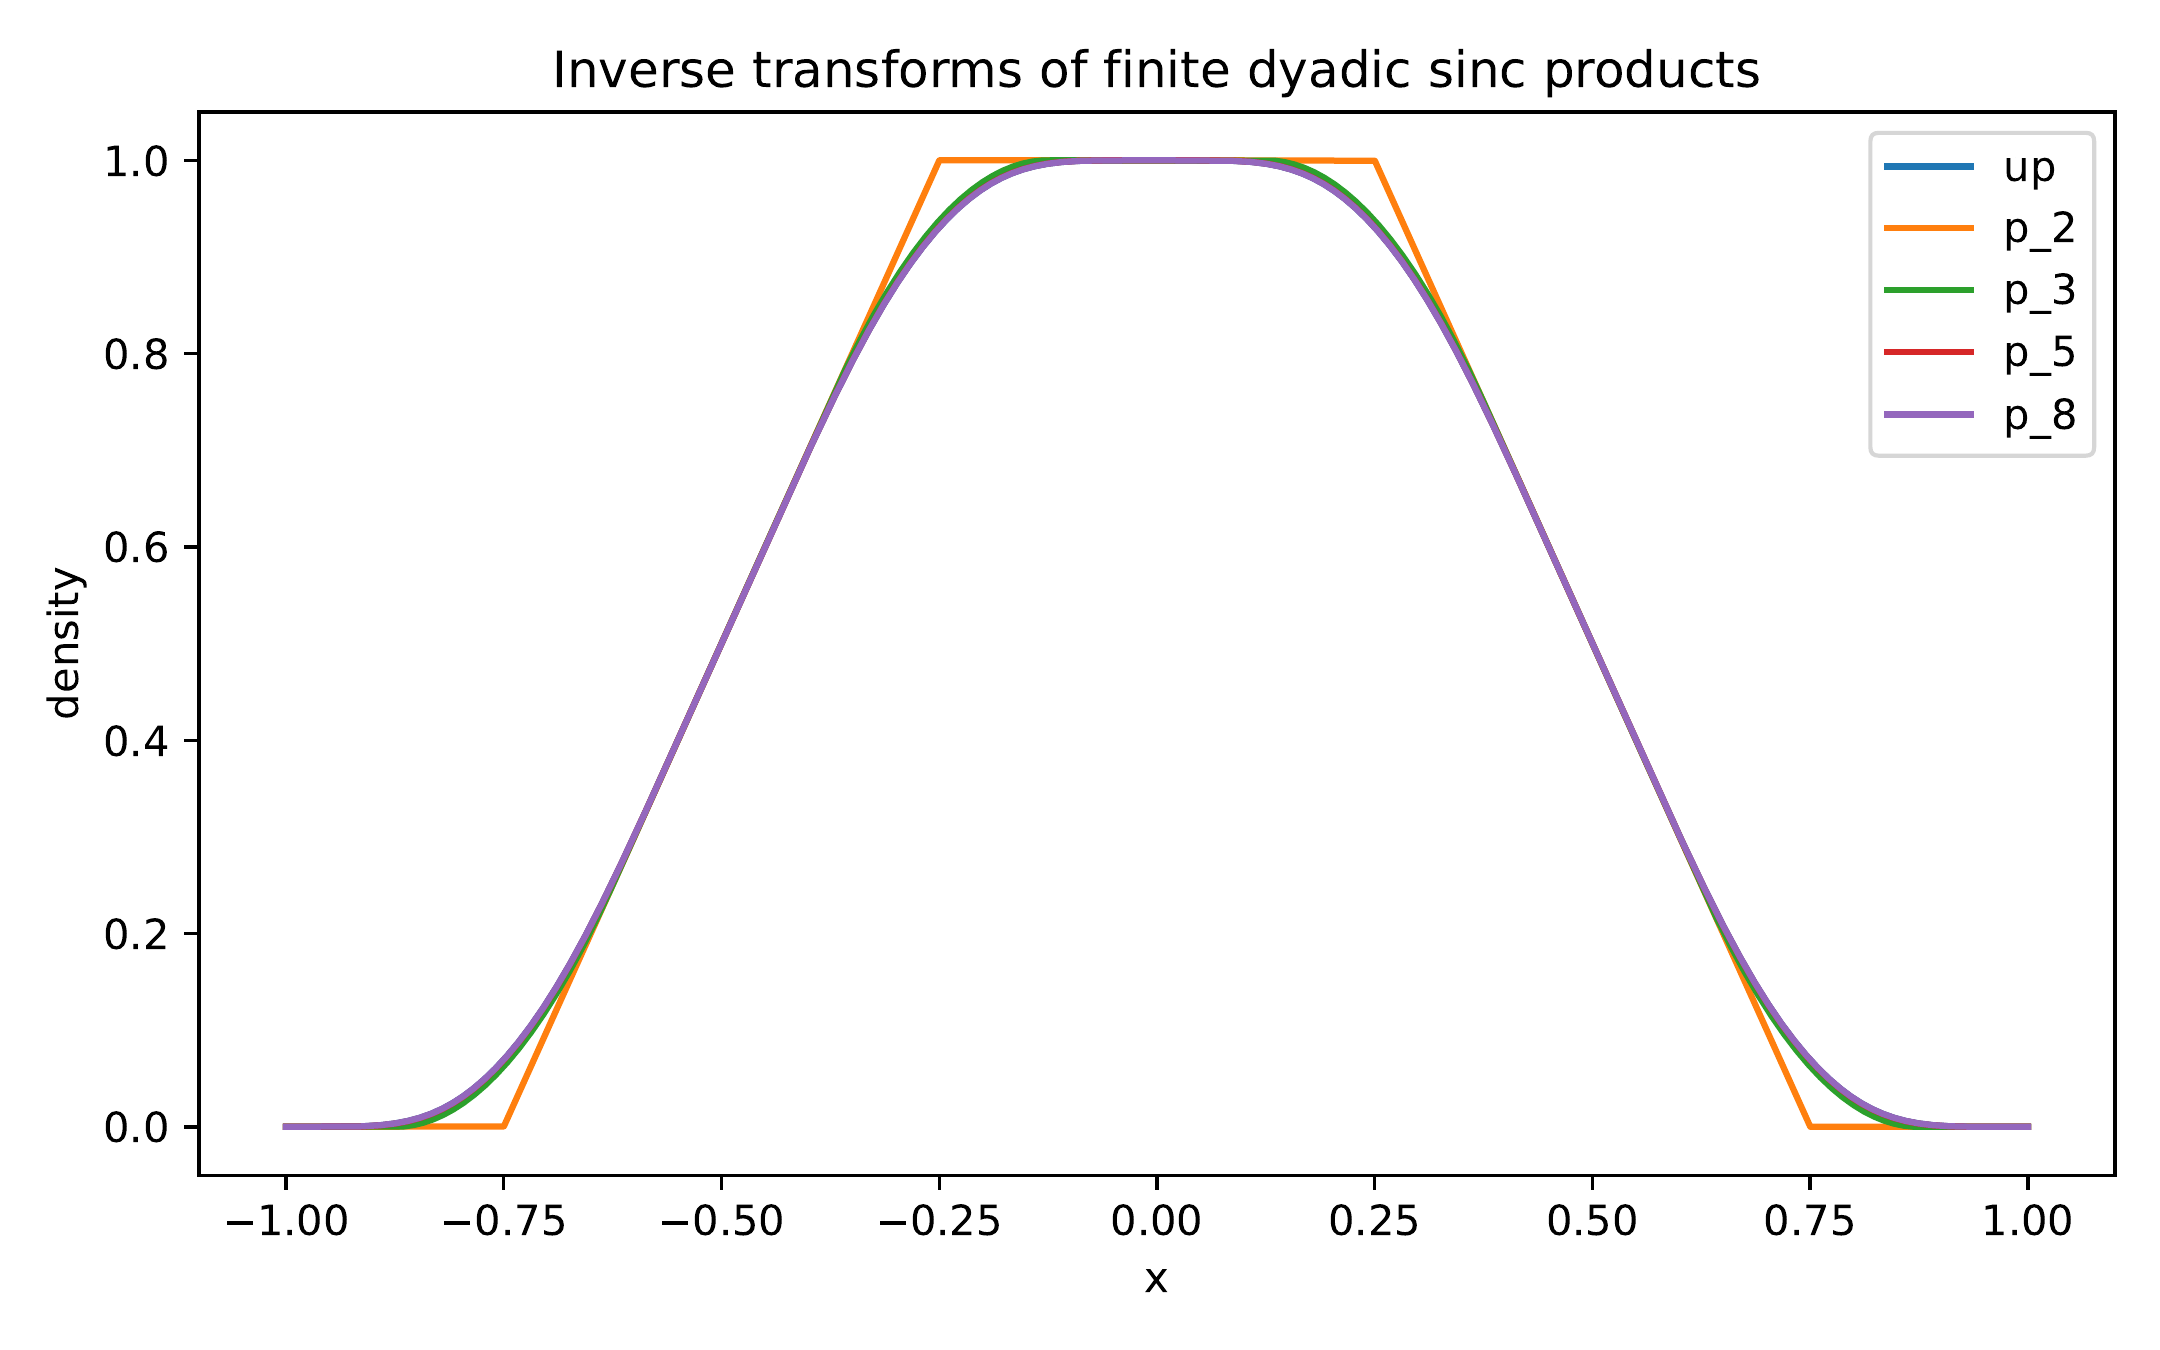
\includegraphics[width=0.88\textwidth]{assets/finite_sinc_products_report/finite_sinc_approximants.png}
\caption{Inverse transforms of the first few finite sinc products.  The support expands
to $[-1,1]$, the polynomial degree and smoothness increase, and the central plateau
shrinks dyadically.}
\label{p3:fig:approximants}
\end{figure}

\begin{figure}[htbp]
\centering
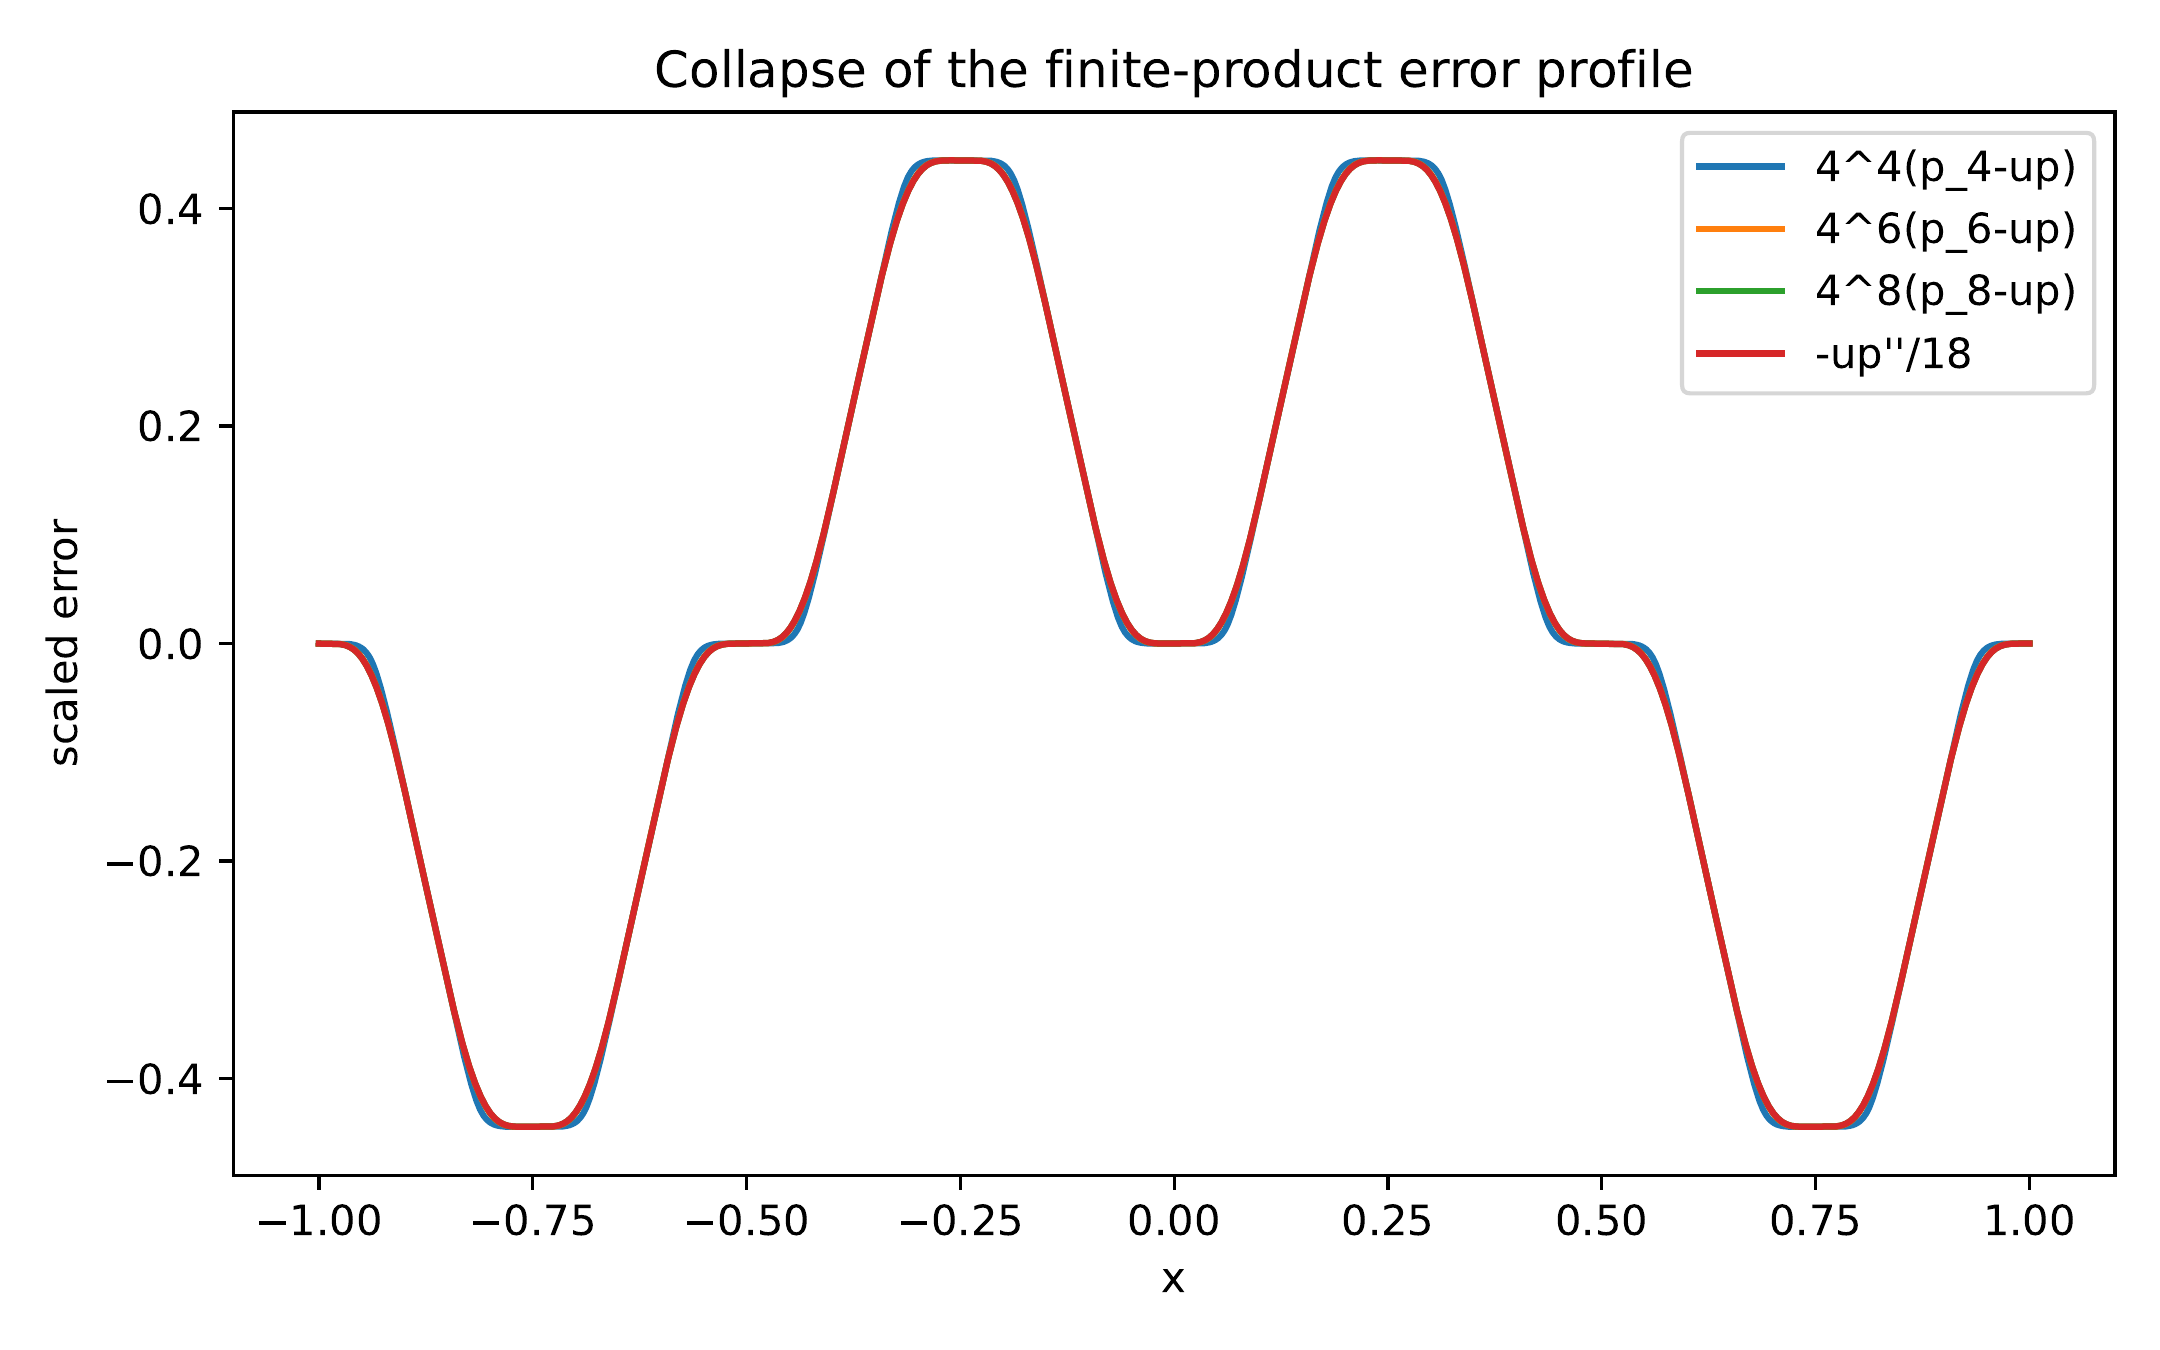
\includegraphics[width=0.88\textwidth]{assets/finite_sinc_products_report/scaled_error_profiles.png}
\caption{The profiles $4^n(p_n-\Up)$ collapse onto $-\Up''/18$, in agreement with
\cref{p3:eq:leading-profile}.}
\label{p3:fig:scaled-errors}
\end{figure}

\begin{figure}[htbp]
\centering
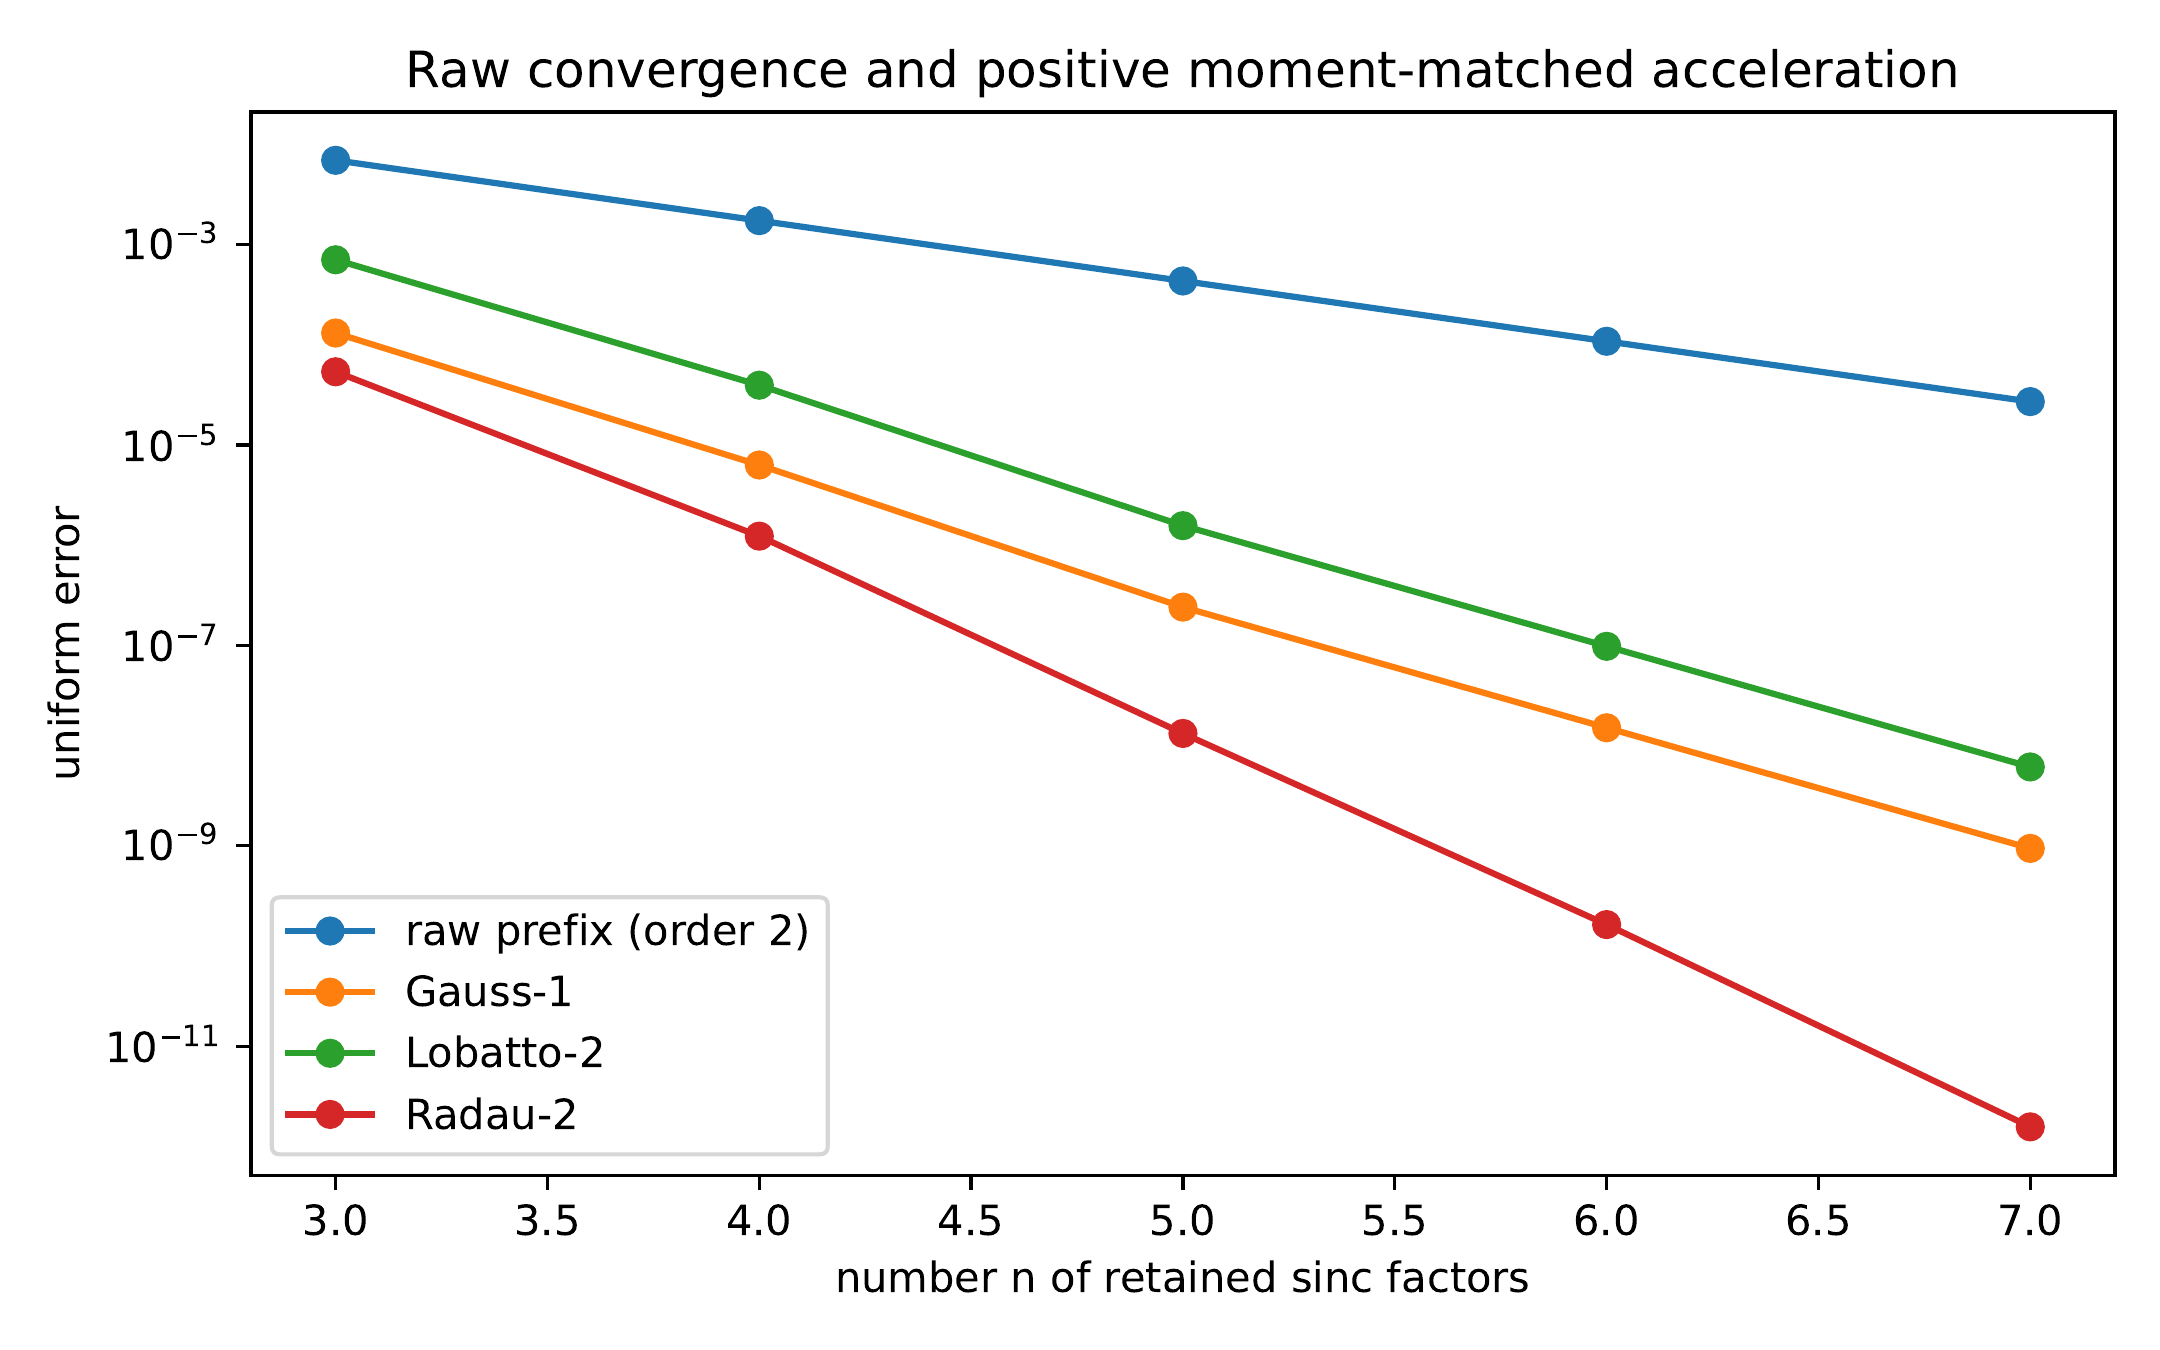
\includegraphics[width=0.88\textwidth]{assets/finite_sinc_products_report/convergence_comparison.png}
\caption{Raw second-order convergence and positive Gauss, Lobatto, and Radau tail
acceleration.  The highest-order Radau values approach the double-precision floor.}
\label{p3:fig:convergence}
\end{figure}

\subsection{Verification of exact constants}

Selected FFT ratios of measured supremum error to the exact formula are shown below.

\begin{center}
\begin{tabular}{@{}lrrrr@{}}
\toprule
Scheme & $r$ & $n$ & measured error & measured/exact\\
\midrule
Raw prefix & 0 & 3 & $6.94444444448\times10^{-3}$ & $1.000000000006$\\
Raw prefix & 2 & 5 & $5.55555555771\times10^{-2}$ & $1.000000000387$\\
Raw prefix & 4 & 7 & $7.11111128754$ & $1.000000024810$\\
Gauss-1 & 0 & 5 & $2.41126543254\times10^{-7}$ & $1.000000000183$\\
Lobatto-2 & 0 & 5 & $1.56732253097\times10^{-6}$ & $1.000000000069$\\
Radau-2 & 0 & 7 & $1.56639950187\times10^{-12}$ & $1.000079775969$\\
\bottomrule
\end{tabular}
\end{center}

The raw and fourth-order laws agree essentially to machine precision.  The Radau error
is already $1.6\times10^{-12}$ at its first admissible $n$, so Fourier truncation and
roundoff visibly affect the last digits.  Full tables are included in
\texttt{sharp\_error\_verification.csv} and
\texttt{positive\_acceleration\_verification.csv}.

\section{Algorithms and implementation considerations}
\label{p3:sec:algorithms}

\subsection{Exact cell construction}

There are three complementary exact representations.

\paragraph{Global truncated powers.}
\Cref{p3:eq:truncated-power} evaluates a point in $O(2^n)$ signed rational % ed.: was "Equation \cref{...}" (doubled word)
operations and is ideal for proof and low-order checks.  Only knots left of $x$ need be
included.

\paragraph{Primitive recursion.}
If a piecewise-polynomial primitive of $p_{n-1}$ is stored cellwise, then
\cref{p3:eq:last-box-recursion} evaluates $p_n$ by two shifted primitive values.  This
constructs the complete spline with exact coefficients while reusing adjacent-cell data.

\paragraph{Top-down integration of the Thue--Morse step.}
Start from the top derivative values in \cref{p3:eq:top-cell-value,p3:eq:tm-prefix}, integrate
cell by cell, and determine constants by continuity and vanishing at the left support
endpoint.  This uses only additions, multiplications by the mesh, and division by small
integers.  It is particularly attractive for formal verification.

\subsection{Positive quadrature construction}

The moment sequence $m_k=(2k+1)\E X^{2k}$ can be generated exactly from the cumulants
\cref{p3:eq:cumulants-X}.  A practical $M$-node Gauss construction is:
\begin{enumerate}[leftmargin=2.1em]
\item compute $m_0,\ldots,m_{2M}$ as rational numbers;
\item perform exact Gram--Schmidt on $1,z,\ldots,z^M$, or solve the Hankel system for
      the monic orthogonal polynomial $P_M$;
\item isolate the $M$ simple roots of $P_M$ in $(0,1)$;
\item solve the Vandermonde moment equations for positive weights;
\item insert the nodes and weights in \cref{p3:eq:gQ-fourier} or
      \cref{p3:eq:gQ-spatial}.
\end{enumerate}
Right-Radau rules are obtained by orthogonalizing against the modified measure
$(1-z)\dd\nu(z)$ and then adjoining $z=1$; Lobatto rules use
$z(1-z)\dd\nu(z)$ and adjoin both endpoints.  Exact rational recurrence coefficients
make certified algebraic output feasible.

\subsection{Numerical stability}

The global formula \cref{p3:eq:truncated-power} contains large alternating terms and should
not be evaluated naively in floating point at high $n$.  Stable options are:
\begin{itemize}[leftmargin=2em]
\item exact rational arithmetic followed by one final conversion;
\item cellwise Horner evaluation after primitive recursion;
\item FFT inversion when values on a dense uniform grid are needed;
\item convolution on adaptive polynomial pieces for positive quadrature mixtures.
\end{itemize}
The Richardson coefficients have uniformly bounded $\ell^1$ norm by
\cref{p3:eq:richardson-stability}; their cancellation is therefore much milder than a
generic high-order extrapolation.  Positive quadrature schemes avoid cancellation
entirely.

\section{Further deductions and research directions}
\label{p3:sec:future}

\subsection{Results that appear immediately accessible}

\begin{problem}[Lean formalization of the prefix law]
Formalize \cref{p3:thm:truncated-power,p3:thm:derivative-plateau,p3:thm:sharp-prefix-law}.
The proof ingredients are already close to the repository's APIs: finite uniform
convolutions, Thue--Morse prefix sums, the exact tail decomposition, bounded weak
second derivatives, and the formally proved sharp derivative tiling of $\Up$.
\end{problem}

\begin{problem}[Certified quadrature generator]
Build an exact-arithmetic pipeline that returns the rational orthogonal polynomial,
certified algebraic nodes, and positive weights for Gauss and right-Radau rules of
$\nu$.  The output would be a library of positive compactly supported approximants with
machine-checkable error constants.
\end{problem}

\begin{problem}[Norms beyond $L^\infty$]
The expansion gives sharp leading constants in every $L^p$ norm.  The exact derivative
distribution identities in the primary exposition suggest that some $L^p$ constants,
rearrangement-invariant norms, or signed error distributions may admit closed forms.
\end{problem}

\subsection{Conjectures}

\begin{conjecture}[$q$-special orthogonal structure]
\label{p3:conj:q-orthogonal}
The monic orthogonal polynomials of
$\dd\nu(z)=-\Up'(\sqrt z)\dd z$ have recurrence coefficients admitting closed
$q$-product or $q$-continued-fraction expressions at $q=1/4$.  Their rationality is
automatic from the rational moments; the conjecture is that the rational numbers have a
simple structural form involving $(q;q)_m$, Gaussian binomials, or the reciprocal-product
coefficients $a_m$.
\end{conjecture}

\begin{conjecture}[Lambert edge scaling of quadrature nodes]
\label{p3:conj:lambert-edge}
The extreme Gauss and Radau nodes have refined endpoint asymptotics controlled by the
same lower-Lambert phase that governs the flat endpoint of the Fabius/Rvachev function.
The leading zero distribution may be classical, but the edge correction should retain
the repository's log-periodic dyadic phase.
\end{conjecture}

\begin{conjecture}[Positive minimax tail rule]
\label{p3:conj:minimax}
Among positive $M$-component uniform scale mixtures supported in $[-1,1]$ and required
to include the endpoint scale $1$, the right-Radau rule minimizes the first nonzero
worst-case $C^r$ error constant simultaneously for all fixed $r$.  The exact plateau
formula reduces this to an extremal moment problem on $[0,1]$.
\end{conjecture}

\begin{conjecture}[Shape preservation]
For every right-Radau rule of $\nu$ and every sufficiently large $n$, the accelerated
density $g_{n,Q}$ is strictly decreasing on $(0,1)$ and has no spurious interior
oscillation.  Positivity is automatic, but monotonicity of a finite mixture is not; a
proof may follow from total positivity of the uniform-box kernel.
\end{conjecture}

\subsection{Broader extensions}

\paragraph{Other geometric bases.}
For $0<q<1$, infinite products generated by widths $(1-q)q^j$ have the same exact
head--tail scaling.  The Bell--Bernoulli expansion and positive tail quadrature survive.
The dyadic case $q=1/2$ is exceptional because subset sums form a uniform grid and the
top derivative is exactly Thue--Morse.  Determining the sharp $C^r$ constants for
general $q$ is a natural next problem.

\paragraph{Multivariate box splines.}
Products of directional sinc factors invert to multivariate box splines.  A geometric
infinite product produces a compactly supported $C^\infty$ atomic function, and finite
prefixes again provide polynomial approximants.  Positive quadrature of the tail scale
may extend with radial or matrix-valued moments.

\paragraph{Inverse Fabius propagation.}
On compact subintervals where $\Up$ is bounded away from zero, the exact error expansion
can be transported through inverse-function calculus to obtain high-order approximations
of the inverse Fabius function.  Near the flat endpoint, the algebraic prefix expansion
must be matched with the Lambert--$W$ asymptotic already developed in the repository.

\paragraph{Spectral and sampling questions.}
The zero multiplicities \cref{p3:eq:zero-multiplicity} suggest dyadic Strang--Fix-type
conditions, multiresolution reconstruction formulas, and exact cancellation identities
for sampled derivatives.  The finite splines could serve as compactly supported
preconditioners whose approximation order is enhanced by the positive tail rules.

\section{Conclusion}

The inverse Fourier transforms of finite dyadic sinc products are much more rigid than
generic finite convolutions.  Binary subset sums force a uniform knot grid; Thue--Morse
signs govern the top derivative; and a precise derivative plateau survives every later
convolution.  Combined with the exact self-similar tail of the Rvachev distribution,
this local geometry turns a Taylor bound into an equality and yields the sharp law
\[
 \norm{p_n^{(r)}-\Up^{(r)}}_\infty
 =\frac{2^{\binom{r+3}{2}-1}}{9\,4^n}.
\]
The same mechanism converts one-signed quadrature errors into exact functional errors.
The resulting Gauss--Radau--Lobatto hierarchy supplies positive piecewise-polynomial
approximants of arbitrary order, with explicit constants and exact support whenever a
right endpoint node is included.  This closes the repository's variance-matched
$16^{-n}$ frontier and opens a tractable new interface among dyadic harmonic analysis,
Thue--Morse combinatorics, Bell--Bernoulli series, orthogonal polynomials, and certified
numerical approximation.

\appendix

\section{Proof of the scale-derivative identity}
\label{p3:app:Ah}

For completeness, we prove \cref{p3:eq:Ah-derivative}.  The case $\ell=0$ is the
definition.  Assume it holds at order $\ell$.  Differentiating under the integral and
using $\partial_z h^{(2\ell)}(\sqrt z u)
=u h^{(2\ell+1)}(\sqrt z u)/(2\sqrt z)$ gives
\[
 A_h^{(\ell+1)}(z)
 =\frac{1}{2^{2\ell+2}\ell!\sqrt z}
 \int_{-1}^{1}u(1-u^2)^\ell h^{(2\ell+1)}(\sqrt z u)\dd u.
\]
Since
\[
 \frac{\dd}{\dd u}(1-u^2)^{\ell+1}
 =-2(\ell+1)u(1-u^2)^\ell,
\]
integration by parts has no boundary term and yields
\[
 A_h^{(\ell+1)}(z)
 =\frac{1}{2^{2\ell+3}(\ell+1)!}
 \int_{-1}^{1}(1-u^2)^{\ell+1}h^{(2\ell+2)}(\sqrt z u)\dd u.
\]
This is the desired induction step.  The formula extends continuously to $z=0$ by
Taylor expansion.

\section{Reproducibility manifest}
\label{p3:app:manifest}

The archive accompanying this report contains:
\begin{itemize}[leftmargin=2em]
\item \path{finite_sinc_products_report.tex} -- the complete source;
\item \path{finite_sinc_products_report.pdf} -- the rendered report;
\item \path{finite_sinc_experiments.py} -- documented numerical and exact code;
\item \path{finite_sinc_approximants.pdf} -- generated approximation figure;
\item \path{scaled_error_profiles.pdf} -- generated error-profile figure;
\item \path{convergence_comparison.pdf} -- generated convergence figure;
\item \path{sharp_error_verification.csv} -- raw-prefix numerical table;
\item \path{positive_acceleration_verification.csv} -- accelerated numerical table;
\item \path{exact_coefficients.txt} -- exact series and Richardson coefficients;
\item \path{exact_rational_samples.csv} -- exact rational spline samples.
\end{itemize}
Run
\begin{lstlisting}[style=reportcode,language=bash]
python finite_sinc_experiments.py --output-dir . --fft-power 17
\end{lstlisting}
to regenerate every figure and table.

\begin{thebibliography}{99}

\bibitem{p3:proveit-primary}
V.~Reshetnikov,
\newblock \emph{The Fabius Function and Rvachev's Up-Function: Exact arithmetic,
probability, Fourier analysis, and corrected sharp asymptotics},
\newblock living TeX exposition in the \texttt{ProveIt} repository, snapshot examined
28 August 2026,
\newblock \url{https://github.com/VladimirReshetnikov/ProveIt/tree/main/Analysis/FabiusFunction/docs/Fabius_Function_and_Rvachev_Up}.

\bibitem{p3:proveit-frontiers}
V.~Reshetnikov,
\newblock \emph{Non-formalized Research Frontiers},
\newblock living consolidated TeX volume in the \texttt{ProveIt} repository, snapshot
examined 28 August 2026,
\newblock \url{https://github.com/VladimirReshetnikov/ProveIt/tree/main/Analysis/FabiusFunction/docs/semi-formalized-research-frontiers}.

\bibitem{p3:proveit-archive}
V.~Reshetnikov,
\newblock \emph{Archive of historical document versions},
\newblock recursive archive index in the \texttt{ProveIt} repository,
\newblock \url{https://github.com/VladimirReshetnikov/ProveIt/tree/main/Analysis/FabiusFunction/docs/archive}.

\bibitem{p3:jessen1935}
B.~Jessen and A.~Wintner,
\newblock Distribution functions and the Riemann zeta function,
\newblock \emph{Transactions of the American Mathematical Society} \textbf{38}
(1935), 48--88.

\bibitem{p3:fabius1966}
J.~Fabius,
\newblock A probabilistic example of a nowhere analytic $C^\infty$-function,
\newblock \emph{Zeitschrift f\"ur Wahrscheinlichkeitstheorie und Verwandte Gebiete}
\textbf{5} (1966), 173--174.

\bibitem{p3:rvachev1971}
V.~L.~Rvachev and V.~A.~Rvachev,
\newblock A certain finite function,
\newblock \emph{Dopovidi Akademii Nauk Ukrains'koi RSR, Series A} (1971),
705--707, 764.

\bibitem{p3:rvachev1990}
V.~A.~Rvachev,
\newblock Compactly supported solutions of functional-differential equations and their
applications,
\newblock \emph{Russian Mathematical Surveys} \textbf{45} (1990), no.~1, 87--120.

\bibitem{p3:arias1982}
J.~Arias de Reyna,
\newblock Definici\'on y estudio de una funci\'on indefinidamente diferenciable de
soporte compacto,
\newblock \emph{Revista de la Real Academia de Ciencias Exactas, F\'isicas y Naturales
de Madrid} \textbf{76} (1982), no.~1, 21--38;
English translation, \emph{An infinitely differentiable function with compact support:
Definition and properties}, arXiv:1702.05442 (2017).

\bibitem{p3:arias2018}
J.~Arias de Reyna,
\newblock Arithmetic of the Fabius function,
\newblock \emph{INTEGERS} \textbf{18} (2018), Article A51;
arXiv:1702.06487.

\bibitem{p3:deboor}
C.~de Boor,
\newblock \emph{A Practical Guide to Splines}, revised edition,
\newblock Springer, New York, 2001.

\bibitem{p3:davis-rabinowitz}
P.~J.~Davis and P.~Rabinowitz,
\newblock \emph{Methods of Numerical Integration}, second edition,
\newblock Academic Press, Orlando, 1984.

\bibitem{p3:gautschi}
W.~Gautschi,
\newblock \emph{Orthogonal Polynomials: Computation and Approximation},
\newblock Oxford University Press, 2004.

\bibitem{p3:allouche-shallit}
J.-P.~Allouche and J.~Shallit,
\newblock \emph{Automatic Sequences: Theory, Applications, Generalizations},
\newblock Cambridge University Press, 2003.

\end{thebibliography}



%% ================= Part IV =================
% ed.: restore arabic section numbering after Part III's appendices
\setcounter{section}{0}
\renewcommand{\thesection}{\arabic{section}}
\part{Fourier Images of the Repeated-Integration Approximants}
% Editorial merge of the two ninth-wave same-topic reports:
%   Rvachev_Piecewise_Approximation_Fourier_Images/
%     Rvachev_Piecewise_Approximation_Fourier_Images.tex
%   rvachev_fourier_frontier_report/
%     rvachev_piecewise_fourier_frontier.tex
% Shared core stated once; unique layers of each source kept; all
% shared constants cross-checked before merging.  See the provenance
% list in the front matter for SHA-256 hashes.

\begin{abstract}
The repeated-integration approximants $f_n$ to Rvachev's up-function
differ from the limit, on the Fourier side, by an exact dilation of a
single universal meromorphic transfer function
$A(z)=\sinc z/\Phi(z)=\prod_{m\ge1}(1-z^2/(\pi^2m^2))^{1-\vtwo(m)}$:
$\widehat{f_n}=\Phi\cdot A(2^{-n}t)$.  The valuation-weighted divisor
of $A$ yields digit-sum zero counts, a Thue--Morse sign law, the exact
Taylor radius $4\pi$ with dominant-pole coefficient asymptotics and an
arithmetic Darboux hierarchy, the complete finite/limit
zero-multiplicity filtration, a sharp $o(2^n)$ relative-convergence
window, forward and inverse conditioning thresholds at $4\pi2^n$ and
$\pi2^n$, and the impossibility of any globally stable convolutional
correction.  All-orders expansions hold in every polynomially weighted
Fourier $L^p$ space and every Sobolev space, with explicit leading
norm constants; the algebraic Fourier tails have exact mean-square
constants and the sharp threshold $f_n\in H^s$ iff $s<n+\tfrac12$.
Interpreting the construction as a tail closure and matching more
moments of the true self-similar tail produces positive
piecewise-polynomial approximants of arbitrary order --- atomic,
dyadic-atomic, and polynomial-density menus with exact constants ---
complementing the box-mixture hierarchy of Part~III.
\end{abstract}

%% ============== Part IV chunk 1: scope + finite objects ==============

\section{Scope, sources, and relation to the prefix theory}
\label{p4:sec:w-scope}

This part is the editorial consolidation of two ninth-wave reports written
independently on the same day and on the same subject --- the global Fourier
geometry of the \emph{repeated-integration} approximants to Rvachev's
up-function:
\emph{Fourier Images of the Piecewise-Polynomial Approximants to Rvachev's
Up-Function} (meromorphic tail transfer, weighted-norm asymptotics,
moment-matched acceleration) and
\emph{Fourier Images of Recursive Piecewise-Polynomial Approximations to
Rvachev's Up Function} ($2$-adic divisors, critical spectral layers, exact
Fourier tails, accelerated closures).  Their shared core --- the transfer
quotient, its cotangent product and divisor, the Taylor radius $4\pi$ and
dominant-pole asymptotics, the finite zero filtration, and the cumulant
defects --- is stated once below with the stronger of the two treatments;
each report's unique layers (respectively: the weighted-$L^p$ master theorem
with its norm constants, the arithmetic Darboux hierarchy, and the
Gauss/Lobatto/polynomial closure menu; the valuation-weighted canonical
product, the digital divisor laws and Thue--Morse sign, the sharp critical
window, the two conditioning thresholds, the deconvolution obstruction, the
exact mean-square tail constants with the sharp Sobolev threshold, and the
dyadic-node closure menu) are kept in full.  Every shared constant was
verified identical between the sources before merging; the two independently
derived zero-order laws, stated in different groupings, agree in all four
valuation regimes.

Where Part~III (\cref{p3:sec:exact-spline}) studies the ordinary prefix
densities $p_n$ in physical space, the present part studies the twin family
$f_n$ (the prefix with its smallest box doubled) on the Fourier side.  The
two theories meet in the closure framework of \cref{p4:sec:w-closures}, where
the three families of accelerated tail surrogates --- the box mixtures of
\cref{p3:sec:positive}, and the atomic and polynomial closures below ---
are compared as quadratures of three different laws.

\emph{Convention.}  This part uses radian frequency,
\begin{equation}
 \widehat g(t)=\int_{\R}g(x)\e^{-\ii tx}\dd x,
 \qquad
 \sinc z=\begin{cases}\sin z/z,&z\ne0,\\1,&z=0,\end{cases}
 \label{p4:eq:w-fourier-convention}
\end{equation}
so that
\begin{equation}
 \Phi(t):=\widehat{\Up}(t)=\prod_{k=1}^{\infty}\sinc\!\left(\frac{t}{2^k}\right),
 \qquad \Phi(0)=1,
 \label{p4:eq:w-phi-def}
\end{equation}
with $\Up$ the even $C^\infty$ probability density on $[-1,1]$.  The
frequency-normalized product used elsewhere in this volume is
$\Phi(2\pi\xi)$; in particular the zeros of \eqref{p4:eq:w-phi-def} sit at
$2\pi m$, $m\in\Z\setminus\{0\}$, with order $1+\vtwo(m)$, and
$\Phi(\pi)=0.5537712758888100953442174163\ldots$ equals the
frequency-normalized product at one half.

\section{The repeated-integration family and its Fourier products}
\label{p4:sec:w-objects}

\subsection{Recursion, box splines, and the head--tail model}

With $f_0=\tfrac12\mathbf 1_{(-1,1)}$, the recursive integration scheme
\begin{equation}
 f_n(x)=2\int_{-1}^{x}\bigl(f_{n-1}(2t+1)-f_{n-1}(2t-1)\bigr)\dd t
 =\int_{2x-1}^{2x+1}f_{n-1}(t)\dd t
 \label{p4:eq:w-recursion}
\end{equation}
produces compactly supported piecewise-polynomial probability densities
converging to $\Up$.  Writing $\beta_a=\tfrac1{2a}\mathbf 1_{[-a,a]}$ for
the centered uniform density and unrolling the recursion,
\begin{equation}
 f_n=\beta_{2^{-1}}*\beta_{2^{-2}}*\cdots*\beta_{2^{-n}}*\beta_{2^{-n}}
 =p_n*\beta_h,
 \qquad h:=2^{-n},
 \label{p4:eq:w-convolution}
\end{equation}
where $p_n=\beta_{2^{-1}}*\cdots*\beta_{2^{-n}}$ is the ordinary prefix of
\cref{p3:sec:exact-spline}: a univariate box spline of degree $n$ supported
on $[-1,1]$, with the smallest box occurring twice.  Probabilistically, if
$X_n$ has density $f_n$, $X$ has density $\Up$, and
$S_n=\sum_{k=1}^{n}2^{-k}U_k$ with $U_k$ independent uniform on $[-1,1]$,
then
\begin{equation}
 X_n\overset d=S_n+hU,
 \qquad
 X\overset d=S_n+hX',
 \qquad X'\overset d=X,
 \label{p4:eq:w-tail-models}
\end{equation}
with all variables independent: the finite construction replaces the true
self-similar tail $hX'$ by a single uniform variable $hU$.  This closure
point of view drives the entire part.

\subsection{Finite products and the master factorization}

With $P_n(t)=\prod_{k=1}^{n}\sinc(t/2^k)=\widehat{p_n}(t)$,
\begin{equation}
 F_n(t):=\widehat{f_n}(t)=P_n(t)\sinc(ht),
 \qquad
 \Phi(t)=P_n(t)\,\Phi(ht).
 \label{p4:eq:w-two-products}
\end{equation}

\begin{definition}[Tail-transfer quotient]
\label{p4:def:w-A}
The \emph{tail-transfer function} (or correction quotient) is the even
meromorphic function
\begin{equation}
 A(z)=\frac{\sinc z}{\Phi(z)},
 \label{p4:eq:w-A-def}
\end{equation}
interpreted at common zeros by meromorphic continuation.
\end{definition}

\begin{theorem}[Master factorization]
\label{p4:thm:w-master}
For every $n\ge1$,
\begin{equation}
 F_n(t)=\Phi(t)\,A(2^{-n}t),
 \label{p4:eq:w-master}
\end{equation}
as an identity of entire functions after the implicit cancellations, and in
the cancellation-free form
$F_n(t)-\Phi(t)=P_n(t)\bigl(\sinc(ht)-\Phi(ht)\bigr)$.
\end{theorem}

\begin{proof}
Divide the two identities in \eqref{p4:eq:w-two-products}.
\end{proof}

All stage dependence is thus an exact dilation of one universal meromorphic
profile: the finite-stage problem separates into the rapidly decaying global
carrier $\Phi(t)$ and the universal microscopic transfer $A(2^{-n}t)$.  The
identity is stronger than an asymptotic statement --- in the renormalized
coordinate $z=2^{-n}t$ the profile
$\mathscr R_n(z)=F_n(2^nz)/\Phi(2^nz)=A(z)$ is independent of $n$, so the
apparent convergence of the finite products is entirely the critical window
moving to infinity, a boundary layer with an exact rather than asymptotic
inner solution.

%% ============== Part IV chunk 2: forms + canonical product + divisor ==============

\section{Exact forms and the canonical valuation product}
\label{p4:sec:w-forms}

\subsection{Functional equations and renormalization products}

The scaling identity $\Phi(2z)=\sinc z\,\Phi(z)$ gives three equivalent
descriptions of the transfer quotient and a dyadic functional equation:
\begin{align}
 A(z)&=\frac{\Phi(2z)}{\Phi(z)^2}
      =\frac{\cos(z/2)}{\Phi(z/2)},
 \label{p4:eq:w-A-forms}\\
 \frac{A(z)}{A(z/2)}
 &=\frac{\sinc z}{\sinc^2(z/2)}
  =\frac z2\cot\frac z2,
 \label{p4:eq:w-A-functional}
\end{align}
the second form of \eqref{p4:eq:w-A-forms} by
$\sinc z=\sinc(z/2)\cos(z/2)$ and one cancellation.  Iterating
\eqref{p4:eq:w-A-functional} from $A(0)=1$ yields the cotangent
renormalization product
\begin{equation}
 A(z)=\prod_{j=1}^{\infty}
 \left(\frac{z}{2^j}\cot\frac{z}{2^j}\right),
 \label{p4:eq:w-cot-product}
\end{equation}
normally convergent on compact pole-free sets since
$u\cot u=1-u^2/3+\bigO(u^4)$; collecting equal cosine scales in
$\sinc z=\prod_{j\ge1}\cos(z/2^j)$ gives the companion form
$A(z)=\cos(z/2)\prod_{j\ge3}\cos(z/2^j)^{-(j-2)}$, which makes the dyadic
pole hierarchy visually transparent.

\subsection{The valuation-weighted canonical product}

The arithmetic structure is clearest in a canonical product obtained by
regrouping Euler's $\sinc z=\prod_{r\ge1}(1-z^2/(\pi^2r^2))$ across the
dyadic scales: a fixed factor $1-z^2/(\pi^2m^2)$ occurs in
$\sinc(z/2^k)$ once for every $k\ge1$ with $2^k\mid m$, i.e.\ $\vtwo(m)$
times in $\Phi$.

\begin{theorem}[Canonical products]
\label{p4:thm:w-canonical}
As an entire function,
\begin{equation}
 \Phi(z)=\prod_{m=1}^{\infty}
 \left(1-\frac{z^2}{\pi^2m^2}\right)^{\vtwo(m)},
 \label{p4:eq:w-phi-canonical}
\end{equation}
and as a meromorphic function,
\begin{equation}
 A(z)=\prod_{m=1}^{\infty}
 \left(1-\frac{z^2}{\pi^2m^2}\right)^{1-\vtwo(m)},
 \label{p4:eq:w-A-canonical}
\end{equation}
both locally uniformly in their natural domains; the exponent sum is
legitimate because
$\sum_m\vtwo(m)m^{-2}<\infty$ (count the multiples of each $2^j$).
\end{theorem}

\subsection{The complete divisor and local principal parts}

\begin{theorem}[Divisor, removable values, and leading jets]
\label{p4:thm:w-divisor}
For every nonzero integer $m$,
\begin{equation}
 \ord_{z=\pi m}A=1-\vtwo(|m|).
 \label{p4:eq:w-divisor}
\end{equation}
Explicitly: $A$ has a simple zero at every odd multiple of $\pi$; the points
$2\pi q$ with $q$ odd are removable with the nonzero values
\begin{equation}
 A(2\pi q)=-\frac1{\Phi(\pi q)};
 \label{p4:eq:w-removable}
\end{equation}
and at $z_0=\pi2^rq>0$ with $q$ odd and $r\ge2$ there is a pole of order
$r-1$ with leading jet
\begin{equation}
 A(z)=-\frac{z_0^{\,r-1}}{\Phi(\pi q)}\,
 (z-z_0)^{1-r}\bigl(1+\bigO(z-z_0)\bigr).
 \label{p4:eq:w-principal-part}
\end{equation}
Equivalently, parametrizing the poles as $z=4\pi q'$ with
$q'\in\Z\setminus\{0\}$, the pole order is $1+\vtwo(q')$.  In particular the
nearest singularities are the simple poles at $\pm4\pi$, with
\begin{equation}
 \Res_{z=4\pi}A=-\frac{4\pi}{\Phi(\pi)}
 =-22.6923481977102997779\ldots,
 \qquad
 \Res_{z=-4\pi}A=+\frac{4\pi}{\Phi(\pi)}.
 \label{p4:eq:w-residues}
\end{equation}
\end{theorem}

\begin{proof}
The order formula is immediate from \eqref{p4:eq:w-A-canonical}.  For the local
jets use $A(z)=\cos(z/2)/\Phi(z/2)$ and put $w=z/2$, $w_0=z_0/2$.  Iterating
the head splitting $r-1$ times,
\[
 \Phi(w)=\Bigl(\prod_{k=1}^{r-1}\sinc(w/2^k)\Bigr)\Phi(w/2^{r-1});
\]
at $w=w_0$ every displayed factor vanishes linearly, all the associated
integer multiples are even except the last, so the product of their sign
slopes is $-1$ and
$\Phi(w)=-\bigl((w-w_0)/w_0\bigr)^{r-1}\Phi(\pi q)(1+\bigO(w-w_0))$.
For $r\ge2$, $\cos(z_0/2)=1$, giving \eqref{p4:eq:w-principal-part}; for $r=1$,
$\cos(\pi q)=-1$ gives \eqref{p4:eq:w-removable}.  The residue at $4\pi$ is the
case $r=2$, $q=1$ of \eqref{p4:eq:w-principal-part}.
\end{proof}

The leading-jet formula \eqref{p4:eq:w-principal-part} evaluates, at every
pole, the top Laurent coefficient in finite terms of $\Phi$ at odd
multiples of $\pi$ --- the first layer of the closed-jet program posed in
\cref{p4:sec:w-directions}.

\begin{figure}[htbp]
 \centering
 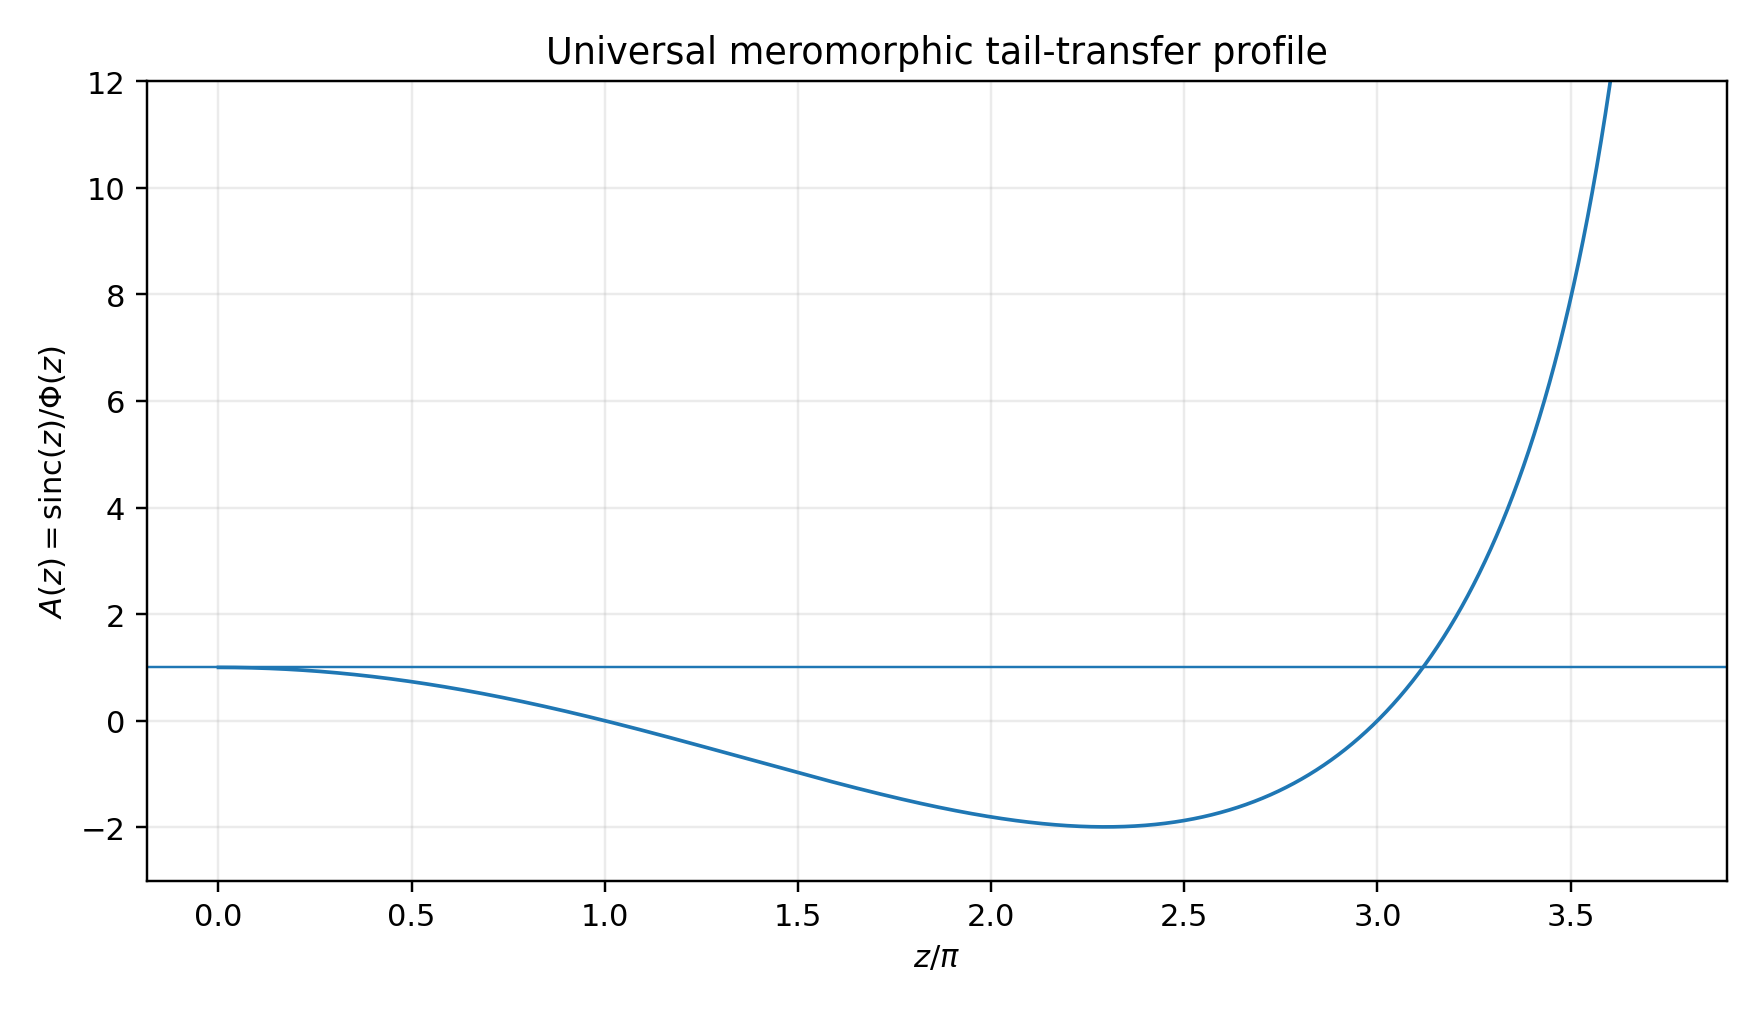
\includegraphics[width=0.92\textwidth]{assets/Rvachev_Piecewise_Approximation_Fourier_Images/data/transfer_profile.png}
 \caption{The universal transfer function on the first positive meromorphic
 cell: simple zeros at $\pi$ and $3\pi$, a removable point at $2\pi$ with
 value $-1/\Phi(\pi)$, and the first pole at $4\pi$.}
 \label{p4:fig:w-transfer-profile}
\end{figure}

\section{Digital divisor laws and the Thue--Morse sign}
\label{p4:sec:w-digital}

The signed divisor sequence $1-\vtwo(m)$ has three exact arithmetic
transforms, and its cumulative parity is a digit sum.

\begin{theorem}[Digital divisor laws]
\label{p4:thm:w-digital}
Let $s_2(M)$ be the binary digit sum.  Then
\begin{equation}
 \sum_{m=1}^{M}\ord_{\pi m}A
 =\sum_{m=1}^{M}\bigl(1-\vtwo(m)\bigr)
 =M-\vtwo(M!)=s_2(M),
 \label{p4:eq:w-digit-sum}
\end{equation}
the total pole multiplicity on $\{\pi,\ldots,M\pi\}$ is
$\lceil M/2\rceil-s_2(M)$, and the divisor has the Lambert and Dirichlet
series
\begin{equation}
\begin{gathered}
 \sum_{m\ge1}(1-\vtwo(m))q^m
 =\frac{q}{1-q}-\sum_{j\ge1}\frac{q^{2^j}}{1-q^{2^j}}
 \quad(|q|<1),\\
 \sum_{m\ge1}\frac{1-\vtwo(m)}{m^s}
 =\zeta(s)\,\frac{2^s-2}{2^s-1}
 \quad(\Re s>1).
\end{gathered}
 \label{p4:eq:w-divisor-series}
\end{equation}
\end{theorem}

\begin{proof}
Legendre's formula $\vtwo(M!)=M-s_2(M)$ gives \eqref{p4:eq:w-digit-sum}; the
pole count is
$\sum_{m\le M}\max\{\vtwo(m)-1,0\}=\sum_{j\ge2}\lfloor M/2^j\rfloor
=\vtwo(M!)-\lfloor M/2\rfloor$.  Since
$\vtwo(m)=\sum_{j\ge1}\mathbf 1_{2^j\mid m}$, summation in $m$ gives both
series, using $\sum_m\vtwo(m)m^{-s}=\zeta(s)/(2^s-1)$.
\end{proof}

\begin{corollary}[Thue--Morse sign law]
\label{p4:cor:w-tm-sign}
For every integer $M\ge0$ and every real $x\in(\pi M,\pi(M+1))$,
\begin{equation}
 \operatorname{sgn}A(x)=(-1)^{s_2(M)}.
 \label{p4:eq:w-tm-sign}
\end{equation}
\end{corollary}

\begin{proof}
$A>0$ near $0$; crossing $\pi m$ flips the sign according to the parity of
the signed order $1-\vtwo(m)$ (poles flip parity exactly as zeros do), and
the cumulative parity through $M$ is $s_2(M)$ by \eqref{p4:eq:w-digit-sum}.
\end{proof}

The Thue--Morse sequence thus appears twice in the theory of the same
splines, by different mechanisms: as subset-sum parity in the spatial
truncated-power coefficients (\cref{p3:eq:truncated-power} for the prefix
family), and as a cumulative valuation divisor in the signs of the universal
Fourier correction.

\begin{figure}[htbp]
 \centering
 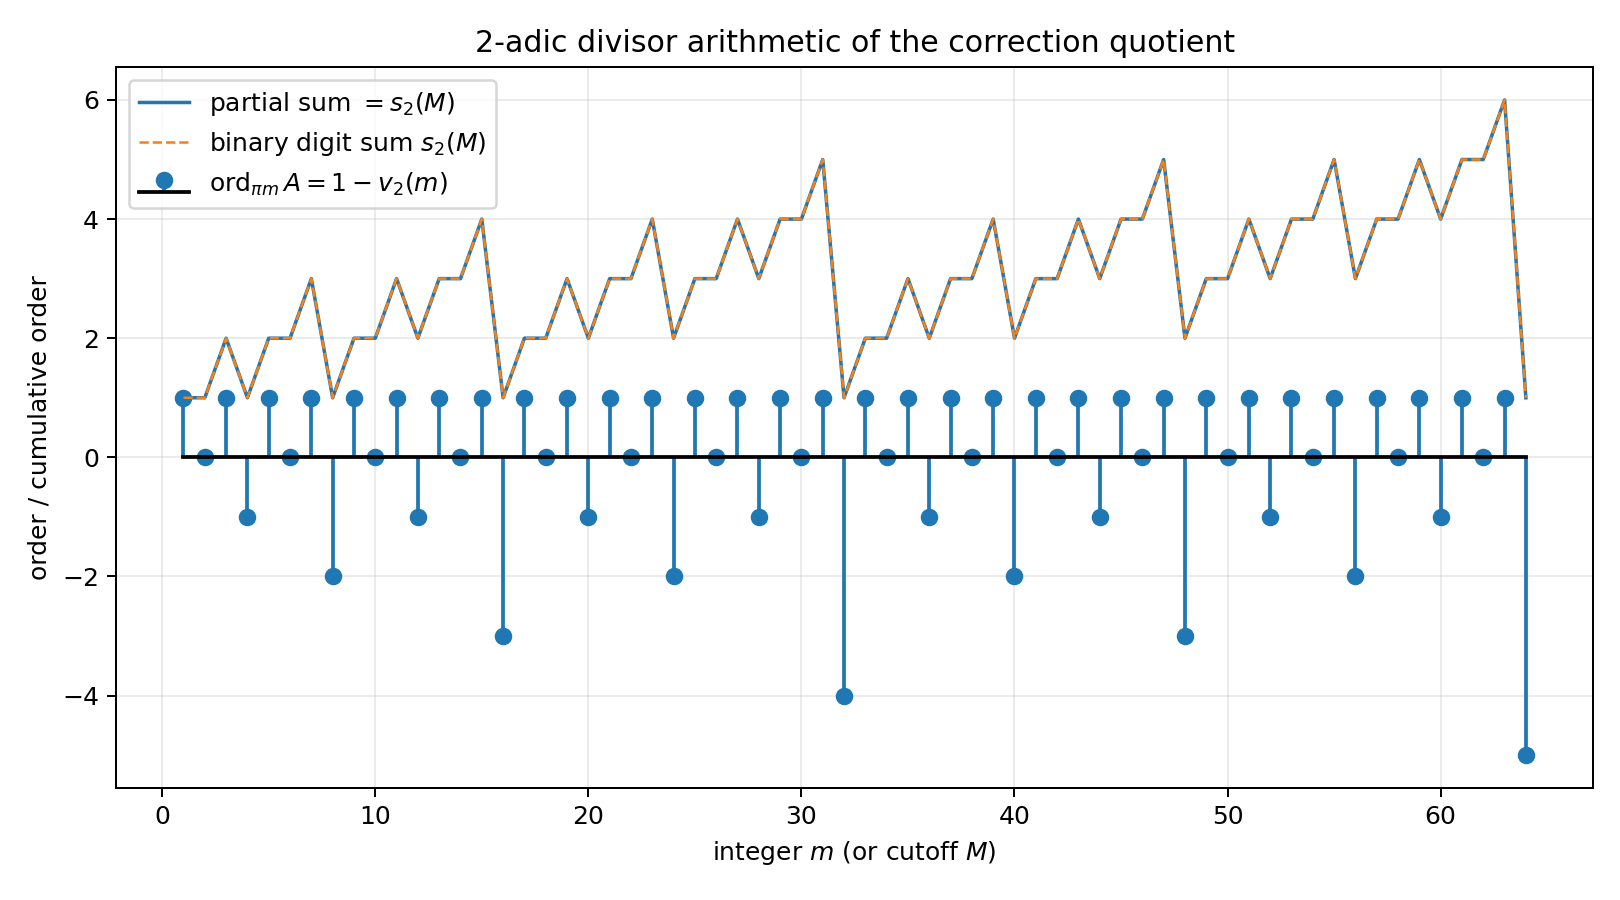
\includegraphics[width=0.94\textwidth]{assets/rvachev_fourier_frontier_report/numerical_output/divisor_arithmetic.png}
 \caption{The signed divisor order $1-\vtwo(m)$ and its cumulative sum,
 which coincides exactly with the binary digit sum $s_2(M)$.}
 \label{p4:fig:w-divisor-arithmetic}
\end{figure}

%% ============== Part IV chunk 3: Taylor coefficients ==============

\section{Taylor coefficients: Bernoulli series, radius, and dominant poles}
\label{p4:sec:w-coefficients}

\subsection{The local logarithm and its arithmetic explanation}

For $|z|<\pi$, the zero-free branch of $\log A$ at the origin is
\begin{equation}
 \log A(z)=\sum_{r=1}^{\infty}\ell_rz^{2r},
 \qquad
 \ell_r=-\frac{2^{2r-1}|B_{2r}|}{r\,(2r)!}\,
 \frac{4^r-2}{4^r-1},
 \label{p4:eq:w-logA}
\end{equation}
the local series already recorded with the repeated-integration corpus.
The canonical product explains its shape arithmetically: logarithmic
expansion of \eqref{p4:eq:w-A-canonical} gives
\begin{equation}
 \log A(z)
 =-\sum_{r=1}^{\infty}\frac{z^{2r}}{r\pi^{2r}}
 \sum_{m\ge1}\frac{1-\vtwo(m)}{m^{2r}}
 =-\sum_{r=1}^{\infty}
 \frac{\zeta(2r)}{r\pi^{2r}}\,\frac{2^{2r}-2}{2^{2r}-1}\,z^{2r},
 \label{p4:eq:w-logA-zeta}
\end{equation}
by the divisor Dirichlet series \eqref{p4:eq:w-divisor-series}; Euler's
evaluation of $\zeta(2r)$ recovers \eqref{p4:eq:w-logA}.  The coefficient
factor $(4^r-2)/(4^r-1)$ is thus the divisor zeta quotient
$\zeta(2r)^{-1}\sum_m(1-\vtwo(m))m^{-2r}$, and simultaneously the exact
$2r$th cumulant defect ratio of \cref{p4:sec:w-cumulants}.

Writing $A(z)=\sum_{r\ge0}\rho_rz^{2r}$, differentiation of
$A=\exp\sum\ell_rw^r$ in $w=z^2$ gives the exact rational recurrence
$r\rho_r=\sum_{k=1}^{r}k\ell_k\rho_{r-k}$, whence
\begin{align}
 A(z)={}&1-\frac{z^2}{9}+\frac{2z^4}{2025}
 +\frac{z^6}{2679075}
 +\frac{58z^8}{10247461875}\notag\\
 &+\frac{12622z^{10}}{345944065438125}
 +\frac{449289436z^{12}}{1933714893977851359375}+\cdots.
 \label{p4:eq:w-A-first-terms}
\end{align}

\subsection{Radius and dominant-pole asymptotics}

\begin{theorem}[Taylor radius and dominant-pole law]
\label{p4:thm:w-radius}
The Maclaurin series of $A$ has radius of convergence exactly $4\pi$: the
zeros at $\pm\pi,\pm3\pi$ do not obstruct analyticity, the points $\pm2\pi$
are removable, and the first genuine singularities are the simple poles at
$\pm4\pi$.  Moreover there is a function $H$ holomorphic in $|z|<8\pi$ with
\begin{equation}
 A(z)=\frac{2/\Phi(\pi)}{1-z^2/(4\pi)^2}+H(z),
 \label{p4:eq:w-pole-split}
\end{equation}
so for every fixed $\rho<8\pi$,
\begin{equation}
\begin{gathered}
 \rho_r=\frac{2}{\Phi(\pi)\,(4\pi)^{2r}}
 +\bigO_\rho(\rho^{-2r}),\\
 \lim_{r\to\infty}\rho_r(4\pi)^{2r}=\frac{2}{\Phi(\pi)}
 =3.6115993860280564486832331013\ldots,
\end{gathered}
 \label{p4:eq:w-rho-asymptotic}
\end{equation}
and $\rho_{r+1}/\rho_r\to(16\pi^2)^{-1}$.  In particular $\rho_r>0$ for all
sufficiently large $r$.
\end{theorem}

\begin{proof}
The paired principal parts at $\pm4\pi$ determined by
\eqref{p4:eq:w-residues} sum to the rational model in
\eqref{p4:eq:w-pole-split}; subtraction removes both first poles, the next
poles are the double poles at $\pm8\pi$, and Cauchy's estimate on
$|z|=\rho<8\pi$ bounds the remainder coefficients.
\end{proof}

Exponentiating the convergent logarithmic series is justified only for
$|z|<\pi$, but the resulting formal recurrence computes the Taylor series of
the meromorphic continuation, convergent throughout $|z|<4\pi$ --- the
ordinary series reaches four times farther than the logarithm.

The dominant-pole approximation is accurate remarkably early: exact rational
computation gives
\begin{center}
\footnotesize
\begin{tabular}{@{}rllllll@{}}
\toprule
$r$ & $3$ & $5$ & $10$ & $20$ & $30$ & $50$\\
\midrule
$\rho_r(4\pi)^{2r}$ & $0.40698$ & $3.58279$ & $3.611538$
 & $3.6115993859$ & $3.611599386028056$ & $3.6115993860280564487$\\
\bottomrule
\end{tabular}
\end{center}
with $\rho_r>0$ verified for $2\le r\le50$.

\begin{proposition}[Arithmetic Darboux hierarchy]
\label{p4:prop:w-darboux}
For $q\ge1$ put $R_q=4\pi q$ and $d_q=1+\vtwo(q)$, and write the principal
part of $A$ at $R_q$ as
$\sum_{\ell=1}^{d_q}c_{q,\ell}(z-R_q)^{-\ell}$.  Then for each $Q\ge1$ and
$R_Q<\rho<R_{Q+1}$,
\begin{equation}
 \rho_r=\sum_{q=1}^{Q}\sum_{\ell=1}^{d_q}
 2(-1)^\ell c_{q,\ell}\,R_q^{-2r-\ell}
 \binom{2r+\ell-1}{\ell-1}
 +\bigO_{Q,\rho}(\rho^{-2r}):
 \label{p4:eq:w-darboux}
\end{equation}
each positive integer $q$ contributes the exponential scale $(4\pi q)^{-2r}$
times a polynomial in $r$ of degree $\vtwo(q)$, so the $2$-adic hierarchy of
pole orders becomes an arithmetic hierarchy of coefficient corrections
\begin{equation}
 \rho_r\sim\frac{2}{\Phi(\pi)(4\pi)^{2r}}
 +\frac{\alpha_1r+\alpha_0}{(8\pi)^{2r}}
 +\frac{\beta_0}{(12\pi)^{2r}}
 +\frac{\gamma_2r^2+\gamma_1r+\gamma_0}{(16\pi)^{2r}}+\cdots,
 \label{p4:eq:w-transseries}
\end{equation}
with the top constant of each block determined by the leading jet
\eqref{p4:eq:w-principal-part}.
\end{proposition}

\begin{proof}
Evenness pairs the principal part at $-R_q$ with signs $(-1)^\ell$; the
coefficient of $z^{2r}$ in a paired principal part is
$2(-1)^\ell c_{q,\ell}R_q^{-2r-\ell}\binom{2r+\ell-1}{\ell-1}$.  Subtract
all paired principal parts with $q\le Q$ and apply Cauchy's estimate in
$|z|<R_{Q+1}$.
\end{proof}

\begin{conjecture}[Global coefficient positivity]
\label{p4:conj:w-positivity}
Apart from $\rho_1=-1/9$, every Taylor coefficient of $A$ is positive.
\end{conjecture}

The dominant-pole law proves this for all large $r$, and exact arithmetic
verifies it through $r=50$, but all nonconstant coefficients of $\log A$ are
negative, so exponentiation produces alternating combinatorial sums and the
finite gap is genuinely open.  Candidate routes: an explicit positive
representation of $A(z)-1+z^2/9$ in $z^2$; a majorization of the negative
logarithmic cumulants after exponentiation; a pole-subtracted
Mittag--Leffler expansion with positivity-preserving remainder; or a
sign-regular interpretation of the tail comparison.

\begin{figure}[htbp]
 \centering
 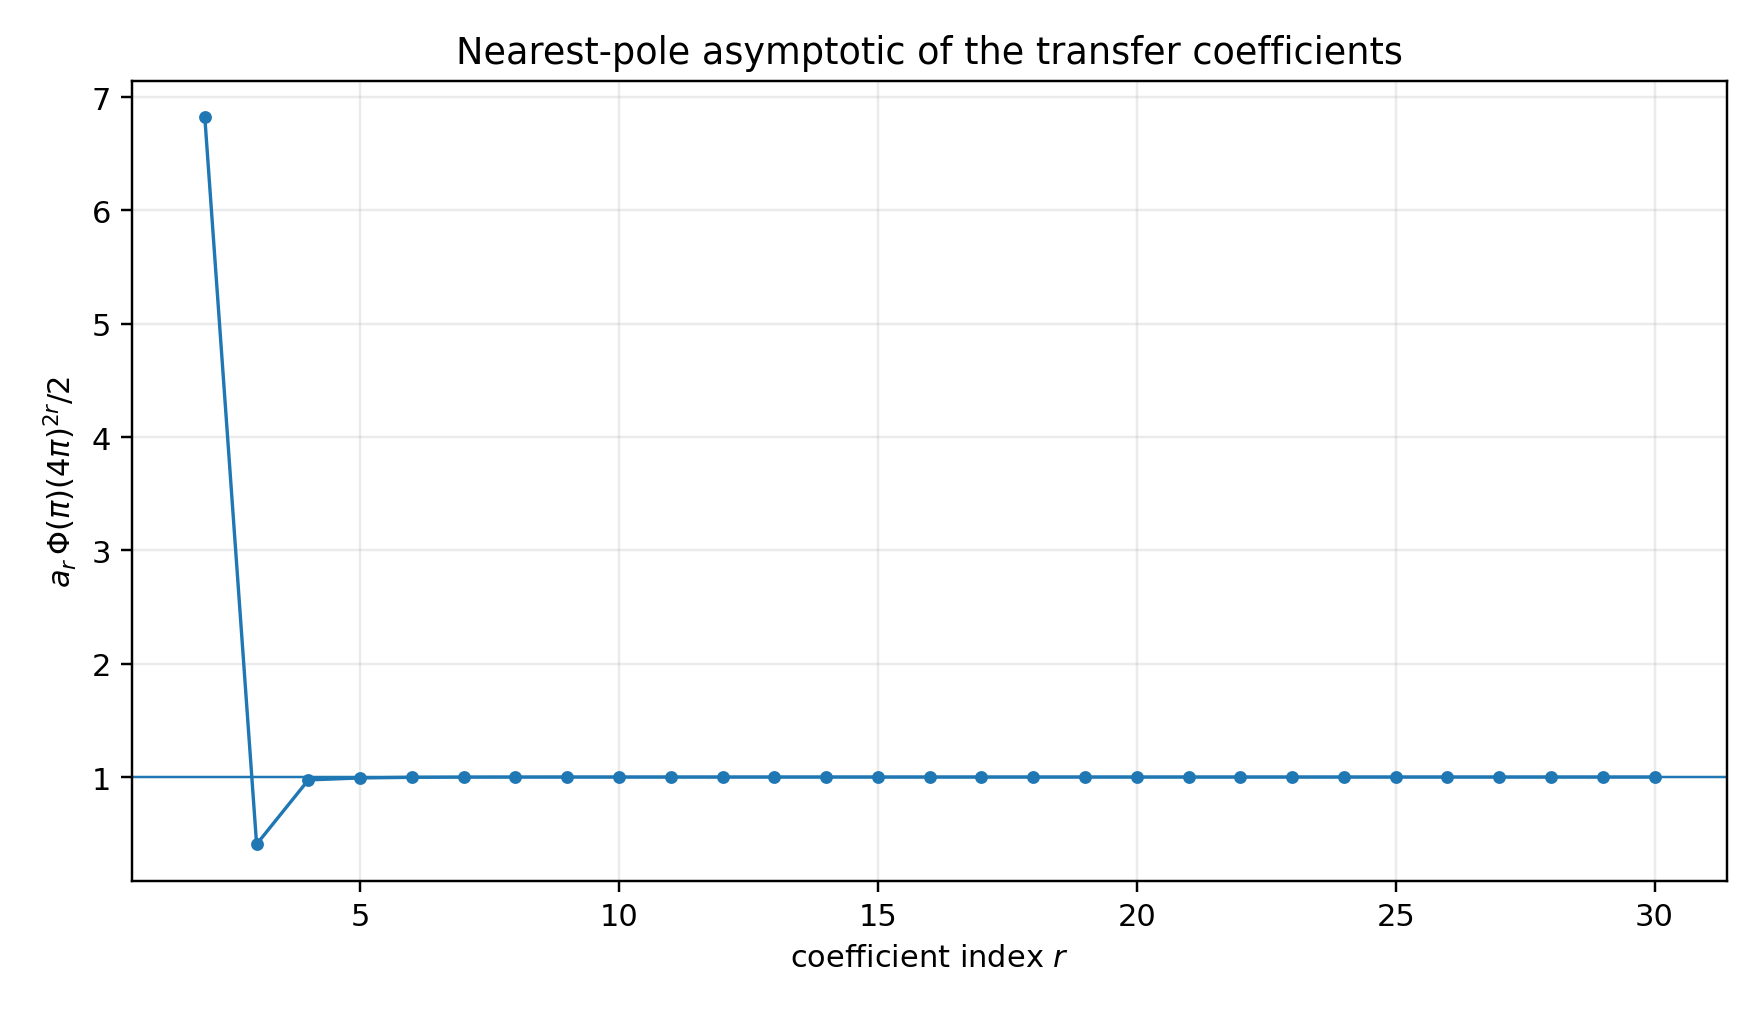
\includegraphics[width=0.9\textwidth]{assets/Rvachev_Piecewise_Approximation_Fourier_Images/data/coefficient_asymptotic.png}
 \caption{Normalized exact rational coefficients
 $\rho_r\Phi(\pi)(4\pi)^{2r}/2$ against the nearest-pole prediction $1$; the
 asymptotic is already highly accurate from $r=4$ onward.  The nearly linear
 semilogarithmic error profile is consistent with the double poles at
 $\pm8\pi$, whose contribution carries a linear polynomial factor in $r$ per
 \cref{p4:eq:w-transseries}.}
 \label{p4:fig:w-coefficient-asymptotic}
\end{figure}

%% ============== Part IV chunk 4: zero filtration + critical layer ==============

\section{The finite zero filtration and its divisor realization}
\label{p4:sec:w-filtration}

Both $F_n$ and $\Phi$ vanish exactly on $2\pi\Z\setminus\{0\}$, but with
different multiplicities --- a distinction invisible in magnitude plots and
precisely responsible for the zeros and poles of the quotient.

\begin{theorem}[Exact finite multiplicities]
\label{p4:thm:w-filtration}
Let $m\in\Z\setminus\{0\}$ and $v=\vtwo(|m|)$.  Then
$\ord_{2\pi m}\Phi=v+1$, while
\begin{equation}
 \ord_{2\pi m}F_n
 =\min(n,v+1)+\mathbf 1_{v\ge n-1}
 =\min(v+1,n-1)+2\cdot\mathbf 1_{v\ge n-1}
 =\begin{cases}
 v+1,&v\le n-2,\\
 n+1,&v\ge n-1.
 \end{cases}
 \label{p4:eq:w-finite-order}
\end{equation}
(The two groupings were derived independently in the two sources, from the
factorizations $F_n=P_n\cdot\sinc(t/2^n)$ and
$F_n=\bigl(\prod_{k<n}\sinc(t/2^k)\bigr)\sinc^2(t/2^n)$ respectively, and
agree in all regimes.)
Consequently the defect
$\Delta_n(m)=\ord_{2\pi m}F_n-\ord_{2\pi m}\Phi$ is
\begin{equation}
 \Delta_n(m)=
 \begin{cases}
 0,&v\le n-2 \quad\text{(exact jet resolution)},\\
 1,&v=n-1 \quad\text{(over-resolved by one order)},\\
 0,&v=n \quad\text{(exact again)},\\
 n-v,&v\ge n+1 \quad\text{(unresolved high dyadic jet)}.
 \end{cases}
 \label{p4:eq:w-defect}
\end{equation}
\end{theorem}

\begin{proof}
$\sinc(t/2^k)$ vanishes at $t=2\pi m$ iff $2^{k-1}\mid m$, i.e.\
$k\le v+1$; among $k=1,\dots,n$ this contributes $\min(n,v+1)$, and the
duplicated smallest box one more exactly when $v\ge n-1$.
\end{proof}

\begin{corollary}[Divisor-level realization]
\label{p4:cor:w-realization}
For every nonzero integer $M$,
$\ord_{t=2^n\pi M}\bigl(F_n/\Phi\bigr)=1-\vtwo(|M|)$: at the critical
scaling $t=2^nz$ the three exceptional layers of \eqref{p4:eq:w-defect} are
exactly the divisor of $A$ --- the over-resolved layer $v=n-1$ is the simple
zero of $A$ at odd multiples of $\pi$, the re-agreement layer $v=n$ is the
removable point at $2\pi\cdot$odd, and each unresolved layer $v\ge n+1$ is
the pole of order $v-n$.
\end{corollary}

\section{The critical spectral boundary layer}
\label{p4:sec:w-critical}

\subsection{The sharp relative-convergence window}

Absolute convergence $F_n\to\Phi$ is strong on the real axis because both
sides decay; relative convergence has an exact scale.

\begin{theorem}[Sharp window criterion]
\label{p4:thm:w-window}
Let $T_n>0$.  With the quotient understood meromorphically,
\begin{equation}
 \sup_{|t|\le T_n}\left|\frac{F_n(t)}{\Phi(t)}-1\right|\longrightarrow0
 \qquad\Longleftrightarrow\qquad
 \frac{T_n}{2^n}\longrightarrow0,
 \label{p4:eq:w-window-iff}
\end{equation}
and in the convergent regime
\begin{equation}
 \sup_{|t|\le T_n}\left|\frac{F_n(t)}{\Phi(t)}-1\right|
 =\frac{T_n^2}{9\cdot4^n}\bigl(1+\bigO((T_n/2^n)^2)\bigr).
 \label{p4:eq:w-window-sharp}
\end{equation}
For fixed $0<c<4\pi$ the critical supremum
$\sup_{|t|\le c2^n}|F_n/\Phi-1|=\max_{|z|\le c}|A(z)-1|$ is independent of
$n$ and nonzero; more generally, truncating the Taylor series of $A$ after
$J-1$ terms leaves a relative error $\bigO(4^{-J\varepsilon n})$ on the
subcritical band $|t|\le2^{(1-\varepsilon)n}$.
\end{theorem}

\begin{proof}
By \cref{p4:thm:w-master}, $F_n/\Phi=A(t/2^n)$.  If $T_n/2^n\to0$, the local
expansion $A(z)=1-z^2/9+\bigO(z^4)$ gives both convergence and
\eqref{p4:eq:w-window-sharp}.  Otherwise a subsequence has
$T_n/2^n\ge\varepsilon>0$, and since $A$ is nonconstant analytic,
$\max_{|z|\le\varepsilon}|A(z)-1|>0$ (infinite if the window reaches a
pole).  The critical identity is a change of variables.
\end{proof}

Hence $2^n$ is not merely a convenient scale but the exact boundary between
uniform relative convergence and a nontrivial limiting profile.

\subsection{Two conditioning thresholds and the deconvolution obstruction}

Bandlimited to $|t|\le c\,2^n$, the exact relation between the finite and
limiting transforms is the Fourier multiplier identity
$\Pi\,f_n=A(2^{-n}D)\,\Pi\,\Up$ with symbol $A(2^{-n}t)$.  Forward
application is governed by the first pole, inversion by the first zero.

\begin{theorem}[Forward and inverse thresholds]
\label{p4:thm:w-conditioning}
Let $M_+(c)=\sup_{|z|\le c}|A(z)|$ and $M_-(c)=\sup_{|z|\le c}|A(z)|^{-1}$.
Then $M_+(c)<\infty$ iff $c<4\pi$, and $M_-(c)<\infty$ iff $c<\pi$, with
the blowup laws
\begin{equation}
 M_+(c)\sim\frac{4\pi}{\Phi(\pi)\,(4\pi-c)}
 \quad(c\uparrow4\pi),
 \qquad
 M_-(c)\sim\frac{\pi\,\Phi(\pi)}{\pi-c}
 \quad(c\uparrow\pi),
 \label{p4:eq:w-blowup}
\end{equation}
the second from the local factorization
$A(z)=\frac{\pi-z}{\pi\Phi(\pi)}(1+\bigO(\pi-z))$ near the first zero
(using $\Phi(\pi/2)=\tfrac\pi2\Phi(\pi)$).
\end{theorem}

\begin{theorem}[No global stable convolutional correction]
\label{p4:thm:w-deconvolution}
There is no compactly supported distribution, finite measure, or $L^1$
kernel $K_n$ with $f_n=\Up*K_n$, and none $L_n$ with $\Up=f_n*L_n$.
\end{theorem}

\begin{proof}
The first identity forces $\widehat{K_n}(t)=A(2^{-n}t)$ everywhere by
meromorphic continuation; the transform of a compactly supported
distribution is entire and that of a finite measure is bounded on $\R$,
while $A(2^{-n}t)$ has a real pole at $4\pi2^n$.  The reverse identity
requires the symbol $1/A(2^{-n}t)$, with a real pole already at $\pi2^n$.
\end{proof}

The obstruction is stronger than ill-conditioning: the global
translation-invariant correction kernel does not exist in any of the usual
stable classes.  Away from the divisor one still has the exact shell
transfer
\begin{equation}
 \log|F_n(2^nz)|-\log|\Phi(2^nz)|=\log|A(z)|,
 \label{p4:eq:w-shell-transfer}
\end{equation}
so every asymptotic decay law for the limiting product on the sequence
$t=2^nz$ transfers to the finite products with an exact $O(1)$ profile
correction --- a direct bridge from the Fourier-decay corpus (which studies
the envelope and transfer-operator behaviour of $\Phi$) to the finite
piecewise-polynomial approximants, to be supplemented at divisor points by
the multiplicity filtration \eqref{p4:eq:w-finite-order}.

\begin{figure}[htbp]
 \centering
 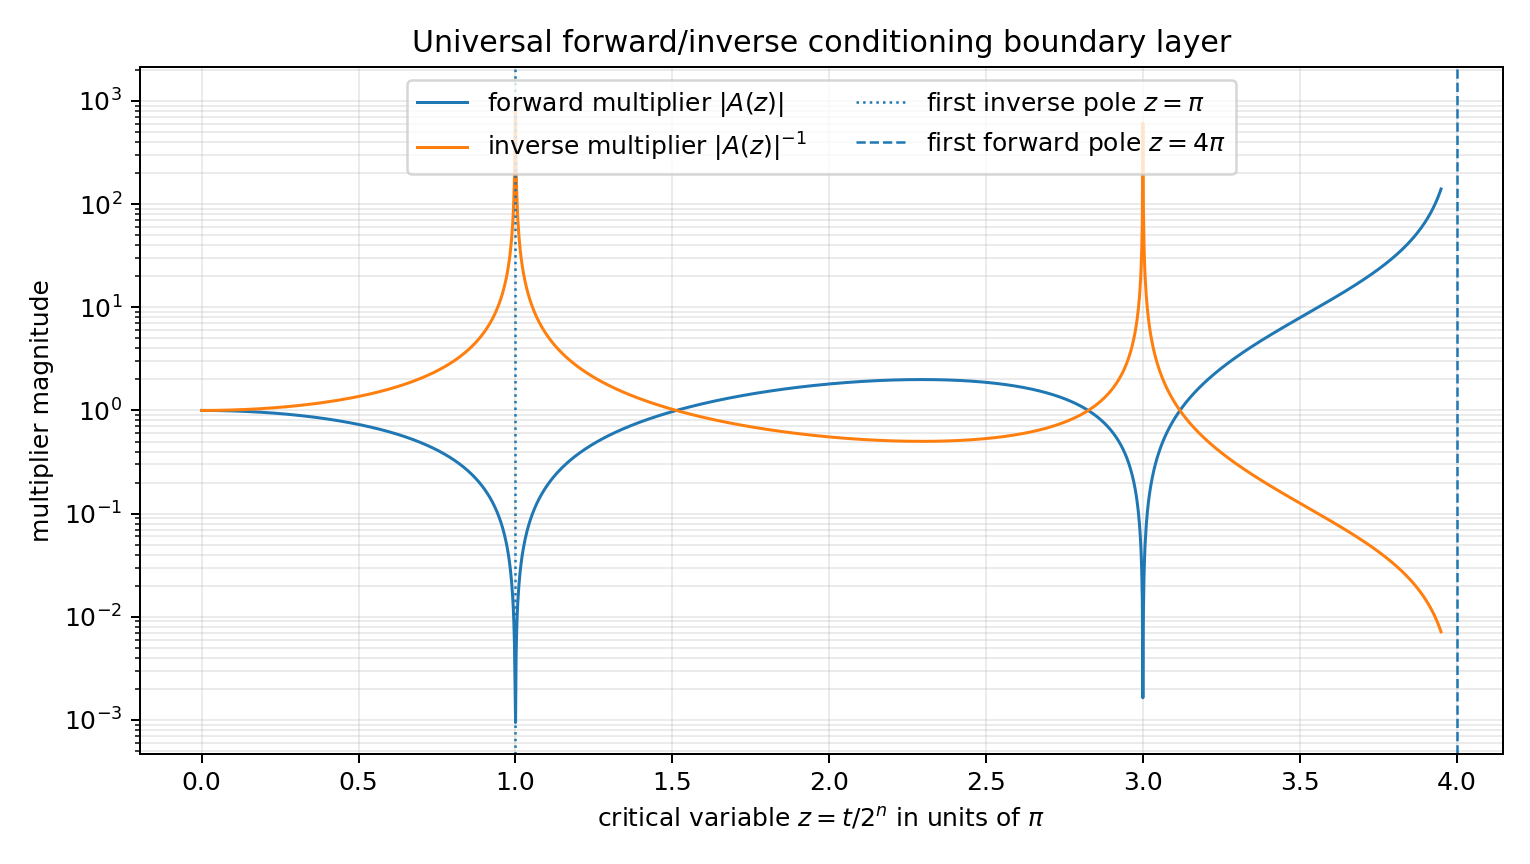
\includegraphics[width=0.92\textwidth]{assets/rvachev_fourier_frontier_report/numerical_output/critical_boundary_layer.png}
 \caption{Forward and inverse multiplier magnitudes on the critical scale
 $z=t/2^n$: inverse instability begins at the first zero $z=\pi$, forward
 instability at the first pole $z=4\pi$, with further inverse peaks at the
 odd multiples of $\pi$.}
 \label{p4:fig:w-conditioning}
\end{figure}

\begin{figure}[htbp]
 \centering
 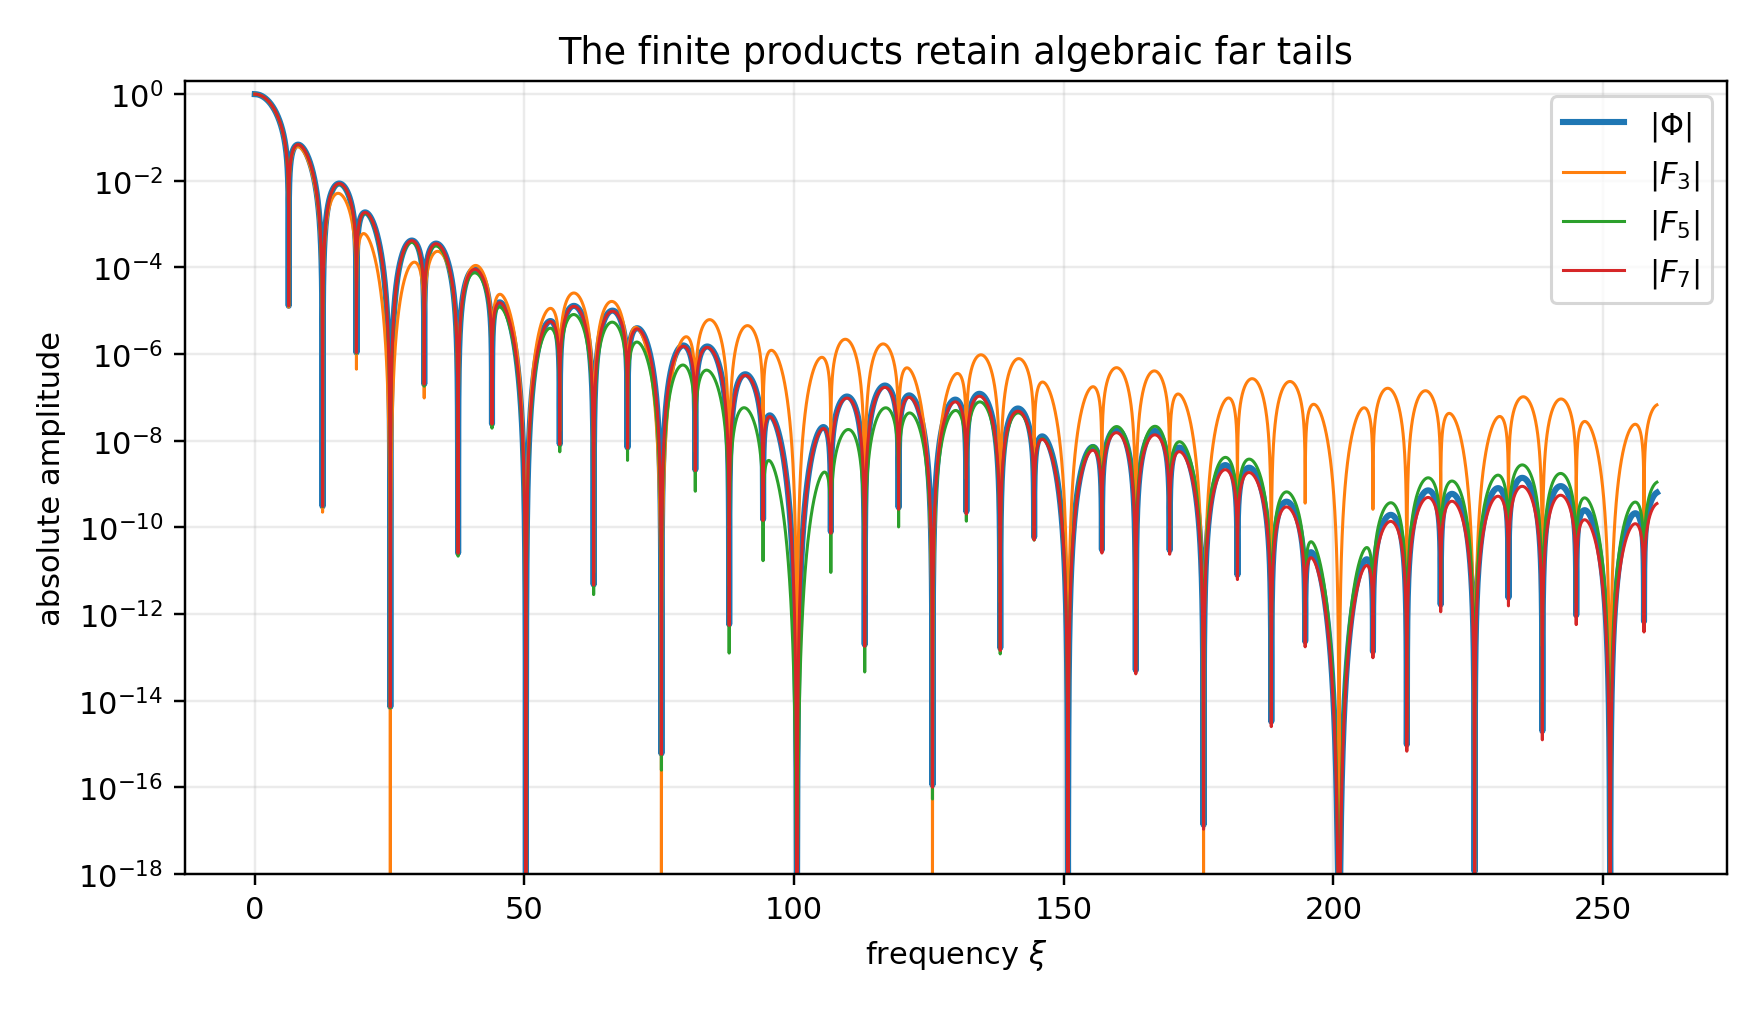
\includegraphics[width=0.94\textwidth]{assets/Rvachev_Piecewise_Approximation_Fourier_Images/data/finite_spectra_log.png}
 \caption{Absolute finite and limiting spectra on a logarithmic scale: each
 fixed finite product has only algebraic far-field decay
 (\cref{p4:sec:w-tails}), while $\Phi$ is rapidly decreasing; increasing $n$
 pushes the discrepancy outward to the boundary layer $|t|\asymp2^n$.}
 \label{p4:fig:w-finite-log}
\end{figure}

%% ============== Part IV chunk 5: norm asymptotics + cumulants + tails ==============

\section{All-orders norm asymptotics}
\label{p4:sec:w-norms}

\subsection{The weighted-\texorpdfstring{$L^p$}{Lp} master theorem}

The local Taylor series of $A$ promotes to a global norm theorem in every
polynomially weighted Fourier space, because the head product supplies
arbitrarily many powers of algebraic decay: for every fixed $N$ and $n\ge N$,
$|P_n(t)|\le\prod_{k=1}^{N}\min(1,2^k/|t|)\le C_N(1+|t|)^{-N}$.  For
$s\ge0$, $1\le p\le\infty$, write
$\norm{g}_{L_s^p}=\norm{(1+|t|)^sg}_{L^p(\R)}$.

\begin{theorem}[Weighted Fourier expansion]
\label{p4:thm:w-weighted}
Let $J\ge1$, $s\ge0$, $1\le p\le\infty$.  As $n\to\infty$,
\begin{equation}
 4^{Jn}\left[
 F_n(t)-\Phi(t)\sum_{j=0}^{J-1}\rho_j4^{-jn}t^{2j}
 \right]
 \longrightarrow \rho_J\,t^{2J}\Phi(t)
 \qquad\text{in }L_s^p(\R),
 \label{p4:eq:w-weighted-limit}
\end{equation}
and hence
$\norm{F_n-\Phi\sum_{j<J}\rho_j4^{-jn}t^{2j}}_{L_s^p}
 =|\rho_J|\,4^{-Jn}\norm{t^{2J}\Phi}_{L_s^p}+\smallo(4^{-Jn})$.
\end{theorem}

\begin{proof}
Let $D_J(z)=\sinc z-\Phi(z)\sum_{j<J}\rho_jz^{2j}$, an entire function with
$D_J(z)=\rho_Jz^{2J}+\bigO(z^{2J+2})$, and let $H_J(z)=D_J(z)/z^{2J}$
(value $\rho_J$ at $0$), continuous and bounded on $\R$ since
$|D_J(z)|\le C_J|z|^{2J}$ for $|z|\ge1$.  The two identities
\eqref{p4:eq:w-two-products} give exactly
\[
 4^{Jn}\Bigl[F_n(t)-\Phi(t)\sum_{j<J}\rho_j4^{-jn}t^{2j}\Bigr]
 =t^{2J}P_n(t)\,H_J(2^{-n}t).
\]
Pointwise, $P_n\to\Phi$ and $H_J(2^{-n}t)\to\rho_J$; choosing
$N>s+2J+1/p$ in the head-decay bound gives an $n$-independent $L^p$
majorant after multiplication by $(1+|t|)^s$, and dominated convergence
concludes.
\end{proof}

\begin{corollary}[Universal leading profile and norm constants]
\label{p4:cor:w-leading}
$4^n(F_n-\Phi)\to-\tfrac{t^2}9\Phi$ in every $L^p_s$, and
$4^n\norm{F_n-\Phi}_{L^p}\to\tfrac19\norm{t^2\Phi}_{L^p}$.  The unweighted
constants, by lobe-wise quadrature, are
\begin{equation}
 C_\infty=\frac19\sup_t t^2|\Phi(t)|=0.650851567393992\ldots
 \quad(\text{maximizer }t_*=3.750573332377785\ldots),
 \label{p4:eq:w-Cinf}
\end{equation}
$C_1=\tfrac19\int t^2|\Phi|\dd t=11.0486184433431\ldots$ and
$C_2=\tfrac19(\int t^4|\Phi|^2\dd t)^{1/2}=2.00390775107366\ldots$
(reproducible numerical values, not certified enclosures); the measured
scaled norms at $n=8$ agree with all three limits to five significant
digits.
\end{corollary}

\subsection{Sobolev expansions, energies, and monotonicity}

Since $\widehat{\Up^{(2j)}}=(-1)^jt^{2j}\Phi$, the $p=2$ case transfers to
physical space: for every fixed real $s\ge0$ and $J\ge1$, with
$a_j=(-1)^j\rho_j$,
\begin{equation}
 4^{Jn}\Bigl[
 f_n-\sum_{j=0}^{J-1}a_j4^{-jn}\Up^{(2j)}
 \Bigr]\longrightarrow a_J\Up^{(2J)}
 \qquad\text{in } H^s(\R)
 \label{p4:eq:w-sobolev}
\end{equation}
(also in every $C^m$ via $p=\infty$) --- the known physical-space expansion
\[
 f_n=\Up+\frac{4^{-n}}9\,\Up''+\frac{2\cdot16^{-n}}{2025}\,\Up^{(4)}
 -\frac{64^{-n}}{2679075}\,\Up^{(6)}+\cdots
\]
is simultaneously an asymptotic
expansion in every fixed Sobolev topology.  On the energy level, with the
convolution coefficients $d_q=\sum_{j=0}^{q}\rho_j\rho_{q-j}$ and
$c_q=\sum_{j=1}^{q-1}\rho_j\rho_{q-j}$, expanding $|F_n|^2=|\Phi|^2A(ht)^2$
gives, for every fixed $s$ and $M$,
\begin{align}
 \norm{f_n}_{\dot H^s}^2
 &=\sum_{q=0}^{M-1}d_q\,4^{-qn}\norm{\Up}_{\dot H^{s+q}}^2
 +\bigO_{s,M}(4^{-Mn})\notag\\
 &=\norm{\Up}_{\dot H^s}^2
 -\frac{2\cdot4^{-n}}9\norm{\Up}_{\dot H^{s+1}}^2
 +\frac{29\cdot16^{-n}}{2025}\norm{\Up}_{\dot H^{s+2}}^2+\cdots,
 \label{p4:eq:w-energy}\\
 \norm{f_n-\Up}_{\dot H^s}^2
 &=\sum_{q=2}^{M-1}c_q\,4^{-qn}\norm{\Up}_{\dot H^{s+q}}^2
 +\bigO_{s,M}(4^{-Mn})\notag\\
 &=\frac{16^{-n}}{81}\norm{\Up}_{\dot H^{s+2}}^2
 -\frac{4\cdot64^{-n}}{18225}\norm{\Up}_{\dot H^{s+3}}^2+\cdots.
 \label{p4:eq:w-error-energy}
\end{align}
Two consequences: the error-norm ratio
$\norm{f_{n+1}-\Up}_{\dot H^s}/\norm{f_n-\Up}_{\dot H^s}\to\tfrac14$, and
$\norm{f_n}_{\dot H^s}$ is eventually strictly increasing to
$\norm{\Up}_{\dot H^s}$ (from the negative $4^{-n}$ term in
\eqref{p4:eq:w-energy}).

\begin{figure}[htbp]
 \centering
 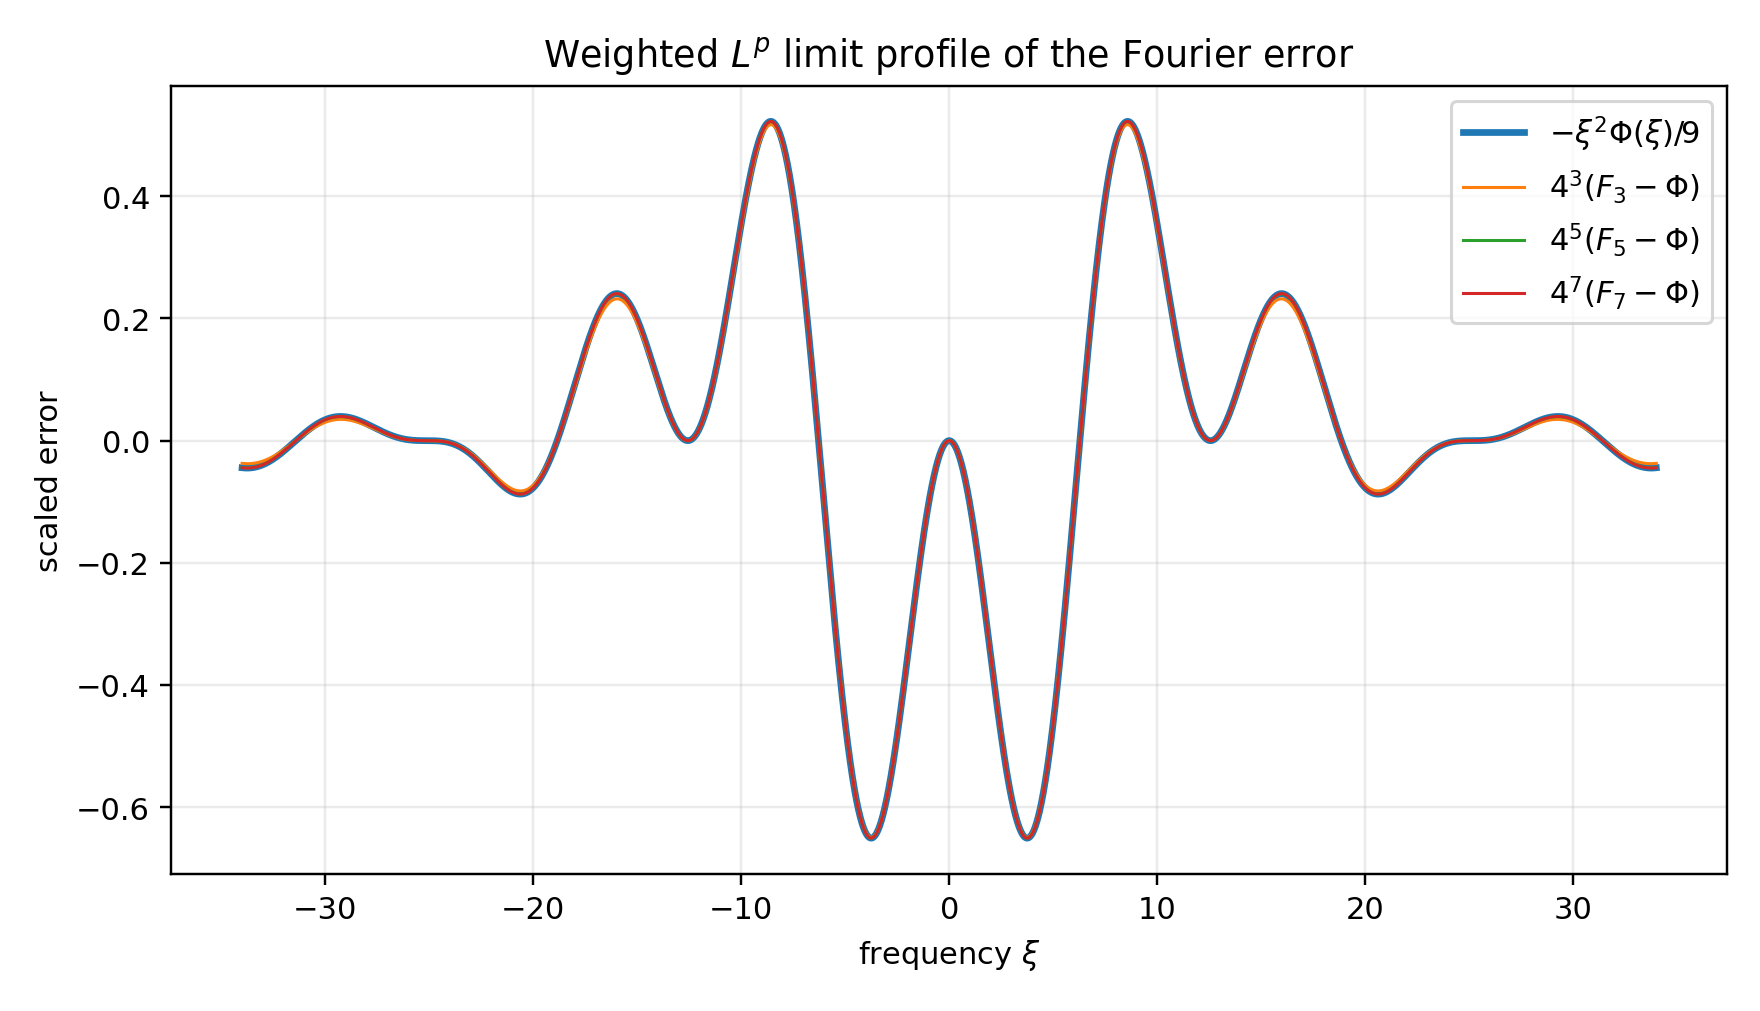
\includegraphics[width=0.94\textwidth]{assets/Rvachev_Piecewise_Approximation_Fourier_Images/data/scaled_fourier_error.png}
 \caption{The scaled errors $4^n(F_n-\Phi)$ converge globally to
 $-t^2\Phi/9$, not only near the origin; \cref{p4:thm:w-weighted} makes the
 convergence valid in every polynomially weighted $L^p$.}
 \label{p4:fig:w-scaled-error}
\end{figure}

\section{Cumulant defects and finite moment polynomials}
\label{p4:sec:w-cumulants}

The transfer function is the quotient of the characteristic function of a
uniform tail by that of the true self-similar tail, so cumulants
diagonalize the comparison: comparing $\log A(ht)$ with the cumulant series
of \eqref{p4:eq:w-tail-models} gives, for every $r\ge1$,
\begin{equation}
 \kappa_{2r}(X)=\frac{2^{2r}B_{2r}}{2r\,(4^r-1)},
 \qquad
 \kappa_{2r}(X_n)-\kappa_{2r}(X)
 =\frac{2^{2r}B_{2r}}{2r}\cdot
 \frac{4^r-2}{4^r-1}\cdot4^{-rn},
 \label{p4:eq:w-cumulant-defect}
\end{equation}
with all odd cumulants zero: the $r$th term of the Bernoulli series
\eqref{p4:eq:w-logA} \emph{is} the defect of the $2r$th cumulant, and the
leading $4^{-n}$ rate is exactly the variance mismatch
$\Var(X_n)-\Var(X)=\tfrac29\,4^{-n}$ between the uniform tail (variance
$\tfrac13$) and the true tail (variance $\tfrac19$).  Bell-polynomial
conversion gives finite-stage moment polynomials in $q=4^{-n}$ of degree at
most the half-order,
\begin{equation}
 \E X_n^2=\frac19+\frac29q,
 \qquad
 \E X_n^4=\frac{19}{675}+\frac4{27}q+\frac{16}{675}q^2,
 \qquad
 \E X_n^6=\frac{583}{59535}+\frac{38}{405}q
 +\frac{16}{405}q^2-\frac{16}{59535}q^3,
 \label{p4:eq:w-moment-polys}
\end{equation}
against the limiting moments
$\E X^2=\tfrac19$, $\E X^4=\tfrac{19}{675}$,
$\E X^6=\tfrac{583}{59535}$, $\E X^8=\tfrac{132809}{32531625}$
(cumulants $\tfrac19$, $-\tfrac2{225}$, $\tfrac{16}{3969}$,
$-\tfrac{16}{3825}$) that determine the accelerated rules of
\cref{p4:sec:w-closures}.

\section{Exact algebraic Fourier tails and the Sobolev threshold}
\label{p4:sec:w-tails}

For fixed $n$ the finite spline has only finite smoothness, visible in the
exact algebraic factorization
\begin{equation}
 F_n(t)=2^{\,n(n+3)/2}\,t^{-(n+1)}
 \Bigl(\prod_{k=1}^{n-1}\sin(t/2^k)\Bigr)\sin^2(t/2^n).
 \label{p4:eq:w-algebraic}
\end{equation}
The oscillatory numerator prevents a pointwise constant, but its mean
square is exactly computable through a dyadic trigonometric integral.

\begin{theorem}[Exact mean-square tail]
\label{p4:thm:w-meansquare}
Let
$I_n=\frac1\pi\int_0^\pi\sin^4u\prod_{j=1}^{n-1}\sin^2(2^ju)\dd u$.  Then
\begin{equation}
 I_n=\frac{2^{n+2}+(-1)^{n+1}}{3\cdot2^{2n+1}},
 \qquad
 I_1=\frac38,\ I_2=\frac5{32},\ I_3=\frac{11}{128},\
 I_4=\frac{21}{512},\ I_5=\frac{43}{2048},\ \ldots,
 \label{p4:eq:w-In}
\end{equation}
and consequently
\begin{equation}
\begin{gathered}
 \lim_{T\to\infty}\frac1T\int_0^Tt^{2n+2}|F_n(t)|^2\dd t
 =2^{n(n+3)}I_n,\\
 \int_{|t|>T}|F_n|^2\dd t
 =\frac{2^{n(n+3)+1}I_n}{2n+1}\,T^{-2n-1}+\bigO_n(T^{-2n-2}),
\end{gathered}
 \label{p4:eq:w-tail-laws}
\end{equation}
with the ideal low-pass error
$\norm{f_n-\Pi_Tf_n}_{\dot H^s}^2
=\frac{2^{n(n+3)}I_n}{\pi(2n+1-2s)}T^{-(2n+1-2s)}+\bigO_n(T^{-(2n+2-2s)})$
for $s<n+\tfrac12$, and the sharp threshold
\begin{equation}
 f_n\in H^s(\R)\quad\Longleftrightarrow\quad s<n+\tfrac12.
 \label{p4:eq:w-Hs-threshold}
\end{equation}
\end{theorem}

\begin{proof}
Let $Q_n(u)=\prod_{j=1}^{n-1}\sin^2(2^ju)$, with constant Fourier
coefficient $2^{1-n}$ and $\cos4u$-coefficient $c_n$.  Since
$\sin^4u=(3-4\cos2u+\cos4u)/8$ and all frequencies of $Q_n$ are multiples
of $4$, $I_n=\tfrac38\,2^{1-n}+\tfrac{c_n}{16}$.  The highest-frequency
coefficient of $Q_n$ is $(-1)^{n-1}2^{3-2n}$ at frequency $2^{n+1}-4$;
multiplying by $\sin^2(2^nu)=(1-\cos(2^{n+1}u))/2$ gives the recurrence
$c_{n+1}=\tfrac{c_n}2-\tfrac{(-1)^{n-1}2^{3-2n}}4$ with $c_2=-\tfrac12$,
solved by $c_n=-\tfrac{2^{2-n}}3-\tfrac{(-1)^n2^{3-2n}}3$; substitution
gives \eqref{p4:eq:w-In}.  The tail laws follow by substituting $u=t/2^n$ in
\eqref{p4:eq:w-algebraic}, averaging the bounded periodic numerator against
$t^{-\alpha}$ by integration by parts, and applying Plancherel; positivity
of $I_n$ makes the weighted integral diverge at $s=n+\tfrac12$, proving
sharpness.
\end{proof}

The threshold is the Fourier counterpart of the spline's final
piecewise-constant derivative stage; \eqref{p4:eq:w-tail-laws} adds the leading
constants, not just the exponents.

%% ============== Part IV chunk 6: closures + comparison ==============

\section{Positive moment-matched closures}
\label{p4:sec:w-closures}

\subsection{The closure framework and the rate theorem}

The construction \eqref{p4:eq:w-tail-models} replaces the exact scaled tail
law by a tractable one --- a \emph{closure}.  For a symmetric probability
measure $\nu$ on $[-1,1]$ with characteristic function
$\psi_\nu(z)=\int\e^{-\ii zx}\dd\nu(x)$, define
\begin{equation}
 g_{n,\nu}=p_n*(D_h\nu),
 \qquad
 \widehat{g_{n,\nu}}(t)=P_n(t)\,\psi_\nu(2^{-n}t),
 \label{p4:eq:w-closure}
\end{equation}
where $D_h$ scales by $h=2^{-n}$.  The original spline is
$\nu=\operatorname{Unif}[-1,1]$; every finitely supported $\nu$ gives a
positive finite sum of shifted head splines
$g_{n,\nu}=\sum_jw_j\,p_n(\,\cdot-2^{-n}t_j)$, a piecewise-polynomial
density of degree $n-1$; a $\nu$ with piecewise-polynomial density of
degree $d$ gives degree at most $n+d$; and the support is exactly $[-1,1]$
iff $\supp\nu$ reaches both endpoints (since
$\supp p_n=[-1+h,1-h]$).

\begin{theorem}[Moment matching determines the spectral order]
\label{p4:thm:w-closure-rate}
If $\int x^k\dd\nu=\E X^k$ for $0\le k\le2M-1$ and
$c_M=\frac{(-1)^M}{(2M)!}\bigl(\int x^{2M}\dd\nu-\E X^{2M}\bigr)\ne0$,
then for every $s\ge0$, $1\le p\le\infty$,
\begin{equation}
 4^{Mn}\bigl(\widehat{g_{n,\nu}}-\Phi\bigr)
 \longrightarrow c_M\,t^{2M}\Phi(t)
 \qquad\text{in }L^p_s(\R),
 \label{p4:eq:w-closure-limit}
\end{equation}
and correspondingly in every $C^m$ and $\dot H^s$ in physical space.
\end{theorem}

\begin{proof}
$\psi_\nu(z)-\Phi(z)=c_Mz^{2M}+\bigO(z^{2M+2})$ by symmetry and Taylor
expansion at $0$; the exact difference is
$P_n(t)(\psi_\nu(ht)-\Phi(ht))$, and the bounded-remainder plus
head-decay argument of \cref{p4:thm:w-weighted} applies verbatim.
\end{proof}

\begin{theorem}[Arbitrary-order positive support-filling closures]
\label{p4:thm:w-existence}
For every $r\ge0$ there is a symmetric, finitely supported probability
measure $\nu_r$ on $[-1,1]$ with positive mass at both endpoints matching
the up moments through degree $2r+1$; consequently
$\norm{g_{n,\nu_r}-\Up}_{C^m}=\bigO_{m,r}(4^{-(r+1)n})$ and likewise in
every $\dot H^s$, with $g_{n,\nu_r}$ nonnegative, of total mass one, and of
support exactly $[-1,1]$.
\end{theorem}

\begin{proof}
Push the up law forward under $x\mapsto x^2$ to a measure on $[0,1]$; a
positive Gauss--Radau rule containing the endpoint $1$ and exact through
degree $r$ exists by standard quadrature theory; lifting each node $y_j$ to
the symmetric pair $\pm\sqrt{y_j}$ with half weights (a zero node to $0$)
gives $\nu_r$.  The rates follow from \cref{p4:thm:w-closure-rate}.
\end{proof}

\subsection{The explicit menu}

Solving the moment equations with the rational moments of
\cref{p4:sec:w-cumulants} yields two complementary explicit families: rules
with minimal atom counts (irrational nodes allowed), and rules with dyadic
rational nodes.  Both sources' overlapping entries agree exactly; the
variance-matched three-point rule below was derived independently in both.

\begin{center}
\small
\begin{tabularx}{\textwidth}{@{}l >{\raggedright\arraybackslash}p{0.33\textwidth} c c >{\raggedright\arraybackslash}X@{}}
\toprule
closure & tail measure $\nu$ & $M$ & $c_M$ & structure\\
\midrule
original uniform & $\operatorname{Unif}[-1,1]$ & 1 & $-1/9$
 & exact support; the spline $f_n$ itself\\
variance box & $\operatorname{Unif}[-1/\sqrt3,1/\sqrt3]$ & 2 & $-1/4050$
 & narrower support; one rescaled box\\
Lobatto--3 & $\tfrac89\delta_0+\tfrac1{18}(\delta_{-1}+\delta_1)$ & 2
 & $7/2025$ & exact support; three shifts\\
Gaussian--3 & $\tfrac{32}{57}\delta_0+\tfrac{25}{114}(\delta_{-a}+\delta_a)$,
 $a=\sqrt{19/75}$ & 3 & $1238/334884375$
 & narrower support; three shifts\\
dyadic--5 & weights $\tfrac{376}{675},\tfrac{896}{2025},\tfrac1{2025}$ at
 $0,\pm\tfrac12,\pm1$ (pair totals) & 3 & $71/21432600$
 & exact support; five dyadic shifts\\
Lobatto--5 & $\tfrac{78976}{153675}\delta_0
 +\tfrac{2470629}{10262075}(\delta_{-b}+\delta_b)
 +\tfrac{619}{270450}(\delta_{-1}+\delta_1)$, $b=\sqrt{683/3087}$ & 4
 & $1006207/24604155961875$ & exact support; five shifts\\
dyadic--7 & pair totals $\tfrac{10411}{2679075},
 \tfrac{1003648}{2679075},\tfrac{581632}{2679075}$ at $\pm1,\pm\tfrac12,
 \pm\tfrac14$, center $\tfrac{120376}{297675}$ & 4 & ---
 & exact support; seven dyadic shifts\\
polynomial $q_3$ & density $\tfrac{35}{32}(1-x^2)^3$ & 2 & $2/22275$
 & exact support; one $C^{n+2}$ density of degree $n+6$\\
\bottomrule
\end{tabularx}
\end{center}

The convergence scales are $4^{-Mn}$: rate $16^{-n}$ for the three
$M=2$ rules, $64^{-n}$ for Gaussian--3 and dyadic--5, $256^{-n}$ for
Lobatto--5 and dyadic--7.  Rules including $\pm1$ preserve the exact
support; Gaussian rules maximize order per atom; the polynomial density
achieves $16^{-n}$ with a single continuous piecewise-polynomial
representation and the smallest leading constant of the $M=2$ entries
($C_{q_3,\infty}=0.0507\ldots$ against $C_{\mathrm{L3},\infty}=1.952\ldots$
and $C_{\mathrm{VB},\infty}=0.1394\ldots$, computed against
$\sup|t|^{4}|\Phi|=564.7796\ldots$ at $t=16.3025\ldots$).  A fixed dyadic
ladder is not guaranteed to retain positivity indefinitely, so
\cref{p4:thm:w-existence} is the robust existence result while the dyadic
menu gives convenient low-order formulas.  Cancellation makes direct
double-precision verification of the $64^{-n}$ and $256^{-n}$ rules
unreliable; the verification packages evaluate the scaled point errors at
$120$ decimal digits and reproduce the predicted leading profiles
(Gaussian--3 at $n=11$: $3.21182$ against the limit $3.21168$;
Lobatto--5 at $n=14$: $873.5187$ against $873.5103$).

\begin{figure}[htbp]
 \centering
 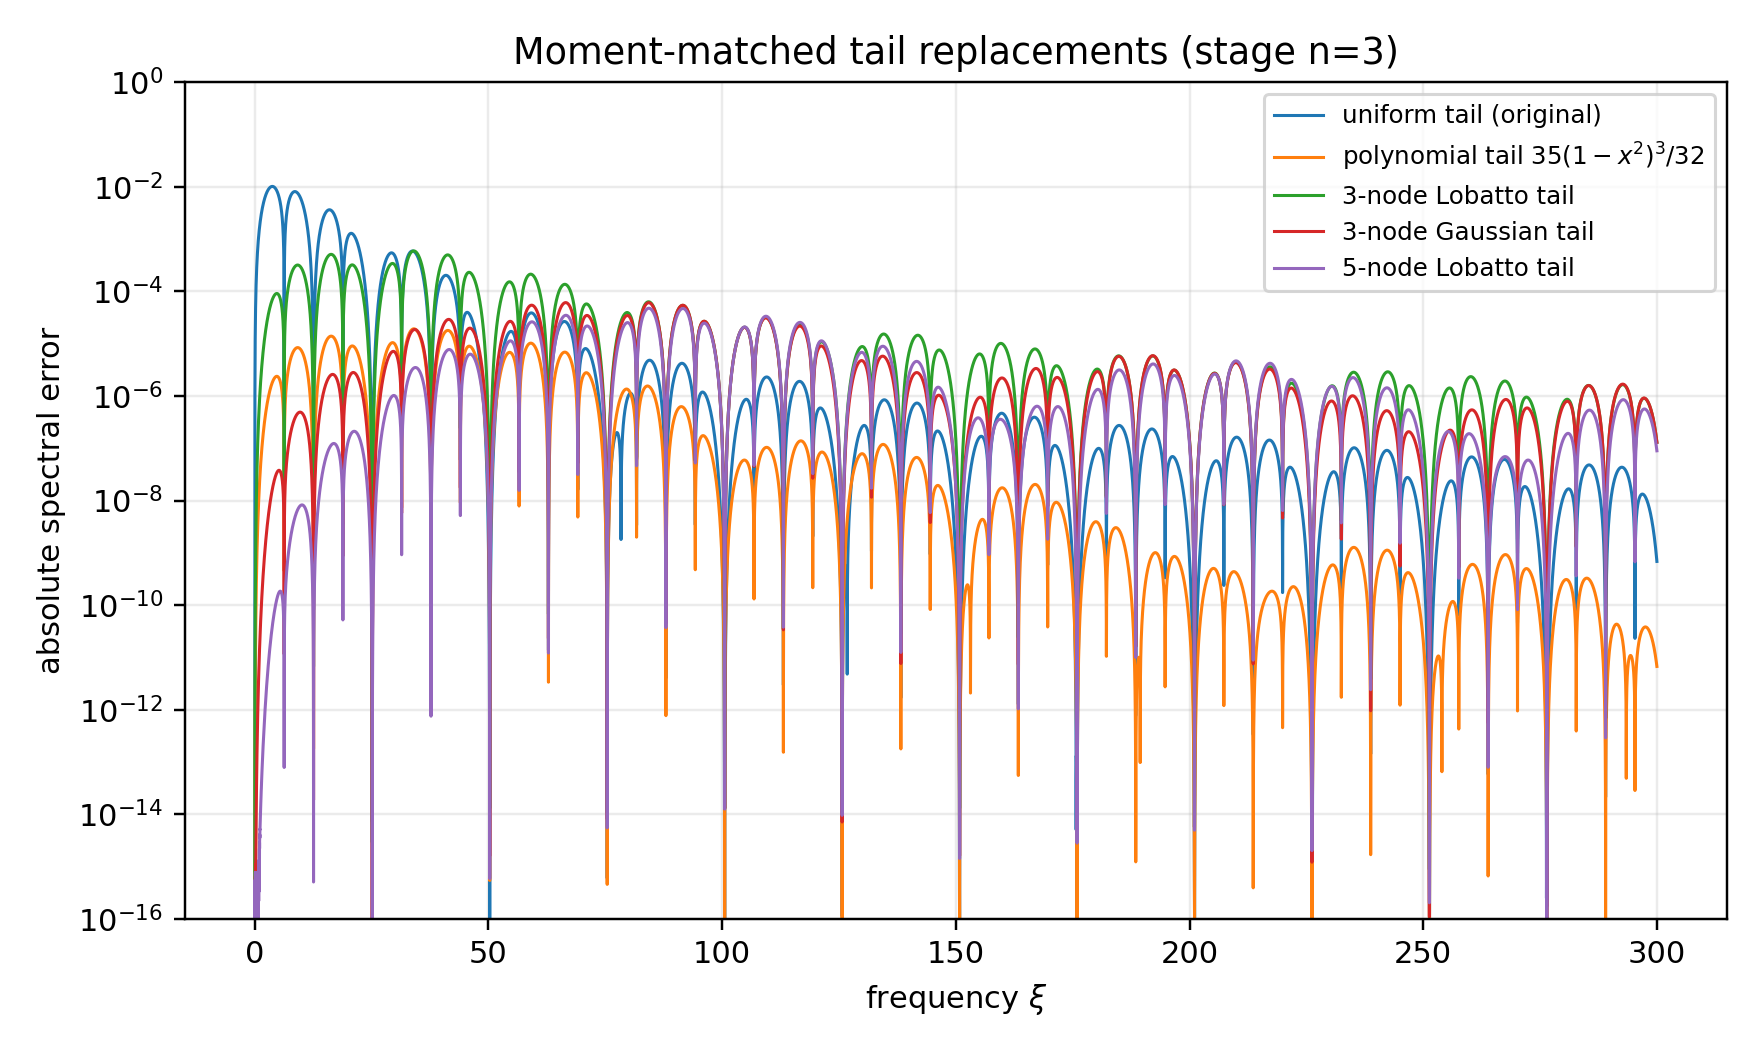
\includegraphics[width=0.94\textwidth]{assets/Rvachev_Piecewise_Approximation_Fourier_Images/data/accelerated_surrogates.png}
 \caption{Absolute Fourier errors of the closure menu at stage $n=3$; the
 faster rates are visible over most of the frequency range, with leading
 profiles attaining maxima on progressively more distant lobes.}
 \label{p4:fig:w-accelerated}
\end{figure}

\subsection{Three closure families and the prefix quadratures}

Part III and this part together produce three structurally different
positive acceleration families over the \emph{same} head spline $p_n$:
\begin{enumerate}
\item \emph{box mixtures} (\cref{p3:eq:gQ-spatial}): quadrature of the
      squared-\emph{scale-mixture} law ($X\overset d=RU$ with
      $Z=R^2\sim\nu$) --- each node contributes a box
      $p_n*u_{\delta\sqrt{z_j}}$, giving mixtures of box splines of full
      degree;
\item \emph{atomic closures} (this part): quadrature of the up law itself
      (equivalently, Gauss--Radau on the pushforward under $x\mapsto x^2$
      lifted symmetrically) --- each node contributes a translate
      $p_n(\cdot-ht_j)$, giving sums of shifted head splines of degree
      $n-1$;
\item \emph{polynomial closures}: a continuous tail density, giving one
      smooth piecewise-polynomial density of slightly higher degree.
\end{enumerate}
The variance-matched members of the first two families have the same
leading constant $|c_2|=1/4050$ --- the box mixture
$p_n*u_{2^{-n}/\sqrt3}$ and the variance box above are the same
approximant seen from the two quadrature variables --- while the
endpoint-preserving members differ genuinely (the box family's Lobatto
rule keeps $p_n$ itself as a component; the atomic family's endpoint atoms
shift the head to $\pm1$).  Moment order controls the global scale
$4^{-Mn}$ in every family; what distinguishes them is support exactness,
smoothness, atom count, and the divisor of the critical transfer
$B_\nu=\psi_\nu/\Phi$, which for generic rules has poles on the full
dyadic zero lattice --- the original uniform tail is special in sharing
many zeros with $\Phi$, which is what produced the removable/pole
hierarchy of \cref{p4:thm:w-divisor}.  Moment order and critical zero
matching are independent design objectives (\cref{p4:sec:w-directions}).

\section{Directions, conjectures, and formalization targets}
\label{p4:sec:w-directions}

\begin{enumerate}
\item \emph{Positivity} (\cref{p4:conj:w-positivity}) and the pole-resolved
      transseries \eqref{p4:eq:w-transseries}: compute the full Laurent jets
      at $4\pi q$ from finite products of $\Phi$-values at odd multiples
      of $\pi$ (the leading jets are \eqref{p4:eq:w-principal-part}),
      reorganize into an optimally truncated arithmetic transseries, and
      decide eventual monotonicity of the normalized ratio.
\item \emph{Hybrid tail design}: for prescribed $M,K$, find positive
      $\nu$ matching moments through $2M-1$ while $\psi_\nu$ shares
      prescribed zero jets with $\Phi$ at $2\pi,\ldots,2\pi K$ ---
      a finite-dimensional positive trigonometric moment problem
      (semidefinite search, then exact certificates); minimize atoms or
      polynomial degree.  Rational or Pad\'e spectral multipliers encoding
      the first poles offer an alternative postprocessing route around the
      kernel obstruction of \cref{p4:thm:w-deconvolution}, with evenness,
      Thue--Morse sign intervals, and no spurious real poles below a
      chosen band as natural constraints.
\item \emph{Optimal closures}: minimize the number of atoms at fixed
      moment order with endpoint masses; minimize the first unmatched
      moment; determine the largest order retaining positivity on a fixed
      dyadic node ladder; minimize the forward multiplier norm on a target
      band (quadrature meets minimax filter design).
\item \emph{Modified local recursions}: derive finite vector-valued
      refinement systems whose $n$th iterate is exactly a Gaussian,
      Lobatto, or polynomial-tail closure, preserving the one-line
      locality of \eqref{p4:eq:w-recursion} at higher order.
\item \emph{Base-$q$ analogues}: for $\Phi_q(z)=\prod_{k\ge1}\sinc(z/q^k)$
      and $A_q=\sinc z/\Phi_q$, the Euler regrouping suggests
      $\ord_{\pi m}A_q=1-\nu_q(m)$ with divisor Dirichlet series
      $\zeta(s)(q^s-2)/(q^s-1)$; determine which spectral and sign
      phenomena survive and which are genuinely binary (for $q=2$ the
      cumulative divisor collapses to the digit sum and the functional
      equation to the cotangent product).
\item \emph{Two-parameter asymptotics}: allow the Fourier weight $s_n$ to
      grow with $n$ and locate the transition between the fixed-weight
      theorem and the exact boundary layer; on the physical side this
      quantifies how much spectral regularity a finite spline possesses at
      a given stage, refining \eqref{p4:eq:w-Hs-threshold}.
\item \emph{Transfer-operator bridge}: insert the shell identity
      \eqref{p4:eq:w-shell-transfer} into the Fourier-decay corpus to obtain
      a joint envelope/profile theorem for finite products, with
      exceptional arithmetic points from \eqref{p4:eq:w-finite-order} and
      uniformity near the first zero and pole.
\item \emph{Lean targets}: the finite multiplicity formula
      \eqref{p4:eq:w-finite-order}; the divisor count and digit-sum identity
      \eqref{p4:eq:w-digit-sum}; the Taylor radius and first residues; the
      $I_n$ recurrence and closed form \eqref{p4:eq:w-In}; the cumulant
      defect \eqref{p4:eq:w-cumulant-defect}; exact moment verification,
      positivity, and support of the explicit closures; and the shift-sum
      identity behind \eqref{p4:eq:w-closure}.  The weighted-$L^p$ theorem is
      modular: a bounded remainder, a finite-product decay lemma, and
      dominated convergence.
\end{enumerate}

\section{Verification and reproducibility}
\label{p4:sec:w-verification}

The two absorbed packages provide independent verification pipelines,
retained verbatim under
\nolinkurl{assets/Rvachev_Piecewise_Approximation_Fourier_Images/} (exact
SymPy coefficients through order $30$, $120$-digit mpmath evaluation of
$\Phi(\pi)$, the residue, and the cancellation-sensitive accelerated
errors, lobe-wise maximization, composite Gauss--Legendre norms on $700$
lobes, symbolic verification of every quadrature rule; figures and CSV
audit artifacts) and
\nolinkurl{assets/rvachev_fourier_frontier_report/} (exact coefficients
through order $50$, functional-identity checks, divisor partial sums
against $s_2$, finite multiplicity tables, $100$-digit quadrature of
$I_n$ against the closed form, rational verification of the dyadic
closures; figures, coefficient CSV, and text summary).  Both scripts
regenerate every figure and table from scratch
(\texttt{fourier\_piecewise\_experiments.py},
\texttt{rvachev\_fourier\_experiments.py}).  All shared constants agree
between the two packages; the numerical work is ancillary throughout ---
every theorem above has a complete proof independent of the computations.


\begin{thebibliography}{9}

\bibitem{p4:AriasTranslation}
J.~Arias de Reyna,
\newblock \emph{An infinitely differentiable function with compact
support: Definition and properties}, English translation of the 1982
article, arXiv:1702.05442 (2017).

\bibitem{p4:Fabius1966}
J.~Fabius,
\newblock A probabilistic example of a nowhere analytic
$C^\infty$-function,
\newblock \emph{Z.~Wahrscheinlichkeitstheorie Verw.~Geb.}
\textbf{5} (1966), 173--174.

\bibitem{p4:Rvachev1990}
V.~A.~Rvachev,
\newblock Compactly supported solutions of functional-differential
equations and their applications,
\newblock \emph{Russian Math.~Surveys} \textbf{45} (1990), no.~1,
87--120.

\bibitem{p4:BoxSplines}
C.~de Boor, K.~H\"ollig, and S.~Riemenschneider,
\newblock \emph{Box Splines}, Applied Mathematical Sciences 98,
Springer, 1993.

\bibitem{p4:Gautschi}
W.~Gautschi,
\newblock \emph{Orthogonal Polynomials: Computation and
Approximation}, Oxford University Press, 2004.

\bibitem{p4:MSE240687}
V.~Reshetnikov,
\newblock Recursive integration over piecewise polynomials: closed
form?,
\newblock Mathematics Stack Exchange, question 240687, 2012.

\end{thebibliography}



%% ================= Part V =================
% Non-duplicate preamble layer for Part V (dead definitions of the
% source preamble dropped; theorem environments and shared letters
% already provided by the volume; \repo re-declared for this part's
% path idiom -- all earlier pages are already typeset).
\newcommand{\eps}{\varepsilon}
\newcommand{\pos}[1]{\left(#1\right)_{+}}
\newcommand{\KL}{\operatorname{D}}
\newcommand{\Ent}{\operatorname{h}}
\newcommand{\Fish}{\operatorname{I}}
\newcommand{\baseline}{\textcolor{linkblue}{\textsf{baseline}}}
\newcommand{\newresult}{\textcolor{deepgreen}{\textsf{proved here}}}
\newcommand{\conjstatus}{\textcolor{deepred}{\textsf{conjectural}}}
\renewcommand{\repo}{\nolinkurl{Analysis/FabiusFunction/docs}}
\newenvironment{proofidea}{\par\smallskip\noindent\textit{Proof architecture.}\ }{\hfill\(\square\)\par\smallskip}
\newenvironment{boxedremark}{%
  \par\smallskip\noindent\begin{center}\begin{minipage}{0.94\textwidth}%
  \color{black}\hrule\vspace{0.6em}\small
}{%
  \vspace{0.6em}\hrule\end{minipage}\end{center}\smallskip
}
% ed.: restore arabic section numbering after Part IV
\setcounter{section}{0}
\renewcommand{\thesection}{\arabic{section}}
\part{Finite Dyadic Sinc Products and Exact Transport Geometry of
Rvachev Spline Approximants}
% Absorbed from fabius_finite_products_frontier/finite_sinc_frontier.tex (tenth wave)

\begin{abstract}
Let
\[
 \Phi_N(\xi)=\prod_{j=1}^{N}\sinc\!\left(\frac{\xi}{2^j}\right),
 \qquad
 \Phi(\xi)=\prod_{j=1}^{\infty}\sinc\!\left(\frac{\xi}{2^j}\right),
 \qquad \sinc z=\frac{\sin z}{z},
\]
and let $u_N$ and $u=\Up$ be their inverse Fourier transforms in the angular-frequency convention.  The established Fabius--Rvachev corpus identifies $u_N$ as a degree-$N-1$ compactly supported spline with a Thue--Morse truncated-power formula and proves strong convergence, an all-orders $4^{-N}$ deconvolution expansion, and signed $q$-Richardson acceleration.  Those facts are used here as input rather than relabelled as new.

The main new result is an exact convergence-geometry package.  Writing $\mu_N=u_N\,\dd x$ and $\mu=u\,\dd x$, we prove that $\mu_N$ increases to $\mu$ in convex order while remaining more peaked about the origin.  The density error crosses zero at the fixed points $\pm\tfrac12$, independently of $N$.  Consequently, for every $N\ge2$,
\[
 W_1(\mu_N,\mu)=d_{\rm K}(\mu_N,\mu)=\frac{4^{-N}}9,
 \qquad
 d_{\rm TV}(\mu_N,\mu)=\frac{2\,4^{-N}}9,
\]
and the stop-loss and order-two Zolotarev distances both equal $4^{-N}/18$.  We also prove $W_\infty(\mu_N,\mu)=2^{-N}$, derive an exact Thue--Morse spline formula for the call potential, and show that its maximum and its total area are both $4^{-N}/18$.  These identities imply a positivity obstruction: no convex combination of consecutive finite-product laws can cancel the leading $4^{-N}$ error in any of the preceding finite metrics; signed weights are structurally necessary for Richardson acceleration.

The report further derives the all-orders stop-loss profile, smooth-test and interior-quantile expansions, and a finite-$p$ versus $p=\infty$ transport crossover.  Fully reproducible FFT experiments verify the exact constants and give strong evidence for new entropy, forward-relative-entropy, Fisher-information, and fixed-$p$ Wasserstein asymptotics.  The latter are explicitly marked conjectural where a weighted endpoint remainder theorem is still required.
\end{abstract}


\section{Audit boundary, status discipline, and contribution map}
\label{p5:sec:audit}

\subsection{Pinned corpus and recursive reading strategy}

The source boundary is the repository commit
\begin{center}
\texttt{21758aba2f8e200342be2a7b321247dac80efc00}
\end{center}
from 28 August 2026.  A recursive inventory of \repo{} returned $95$ paths with extension \texttt{.tex}.  The tree contains the canonical exposition, imported papers, historical archive copies, a living consolidated frontier volume, and current thematic draft consolidations.  Reading every historical revision as an independent mathematical source would overcount the same theorem many times.  Accordingly, the audit followed the repository's own consolidation policy:

\begin{enumerate}
\item inventory every \texttt{.tex} path recursively;
\item read the canonical exposition and the consolidated frontier volume as the current mathematical spine;
\item read the live draft manifest and every topic-specific source capable of overlapping finite sinc products, splines, $q$-Richardson acceleration, transport, entropy, or multiresolution analysis;
\item normalize archived duplicates against their live successor and use imported papers as literature baselines rather than repository discoveries;
\item run formula-level searches for the proposed new invariants: convex order, peakedness, single crossing, stop-loss, Zolotarev, exact Wasserstein/Kolmogorov/TV constants, and positive-mixture obstructions.
\end{enumerate}

This is the same cumulative-audit methodology used by the recent frontier reports.  The phrases ``proved here'' and ``new'' below mean that no explicit counterpart was located in the pinned corpus after the preceding source- and formula-level audit.  They do not assert exhaustive worldwide priority.

\subsection{Established material deliberately excluded from novelty claims}

\begin{longtable}{@{}>{\raggedright\arraybackslash}p{0.25\textwidth}>{\raggedright\arraybackslash}p{0.68\textwidth}@{}}
\toprule
Layer & Audited prior material used as input \\
\midrule
\endfirsthead
\toprule
Layer & Audited prior material used as input \\
\midrule
\endhead
Function theory & Existence, uniqueness, support, symmetry, positivity, flatness, refinement equations, and the relation between the bounded Fabius CDF and the even up-density.\\
Probability & Weighted sums of independent uniform variables, finite atomic and finite spline laws, exact tail coupling, reflection, and weak/strong convergence.\\
Finite splines & Thue--Morse truncated-power formulas, exact dyadic knots, repeated-integration formulas, support bounds, and exact rational evaluation at dyadic points.\\
Fourier analysis & Infinite and finite sinc products, local uniform convergence, Fourier inversion, rapid decay, zeros and multiplicities, Poisson summation, and cosine sampling formulas.\\
Asymptotics & The logarithmic tail expansion in powers of $4^{-N}$, Bell--Bernoulli coefficient algebra, all-orders physical-space expansion, and zero-preserving signed $q$-Richardson acceleration.\\
Endpoint theory & Correct lower-Lambert coordinate, nonconstant periodic Gamma--zeta phase, and all-orders endpoint and inverse-endpoint expansions.\\
Multiresolution & Haar and Faber--Schauder expansions, exact energy tails, Bernstein/Kummer representations, and weighted-cube geometry.\\
\bottomrule
\end{longtable}

The finite-spline construction and the $q$-Richardson machinery are therefore restated only compactly enough to make the new deductions self-contained.

\subsection{New theorem package}

The proved contribution is the following linked package.

\begin{enumerate}
\item \newresult: a convex-order chain $\mu_N\preceq_{\rm cx}\mu_{N+1}\preceq_{\rm cx}\mu$ together with a peakedness chain for all centered intervals;
\item \newresult: the exact moment identity
\[
 \E\abs{X_N}=\frac5{18}-\frac{4^{-N}}9;
\]
\item \newresult: a fixed single-crossing law for $u_N-u$, with crossings at $0$ and $\pm\tfrac12$ and no $N$-dependent drift;
\item \newresult: exact $W_1$, Kolmogorov, total-variation, stop-loss, Zolotarev, and $W_\infty$ errors, including the sole first-stage exception;
\item \newresult: an exact piecewise-polynomial call/put potential and an all-orders profile whose leading term is $u/18$;
\item \newresult: an exact no-go theorem for positive mixture acceleration in all the preceding finite metrics;
\item \newresult: monotone entropy and Fisher-information facts, including the exact criterion $\Fish(u_N)<\infty\iff N\ge3$ and the exact divergence $\KL(u\Vert u_N)=\infty$;
\item \conjstatus: weighted endpoint expansions for entropy, forward KL, Fisher information, and fixed finite-$p$ Wasserstein distance, supported by high-resolution computations.
\end{enumerate}

\section{Normalization and the common probability space}
\label{p5:sec:model}

\subsection{Fourier convention}

Throughout the report,
\begin{equation}
 \widehat f(\xi)=\int_{\R}f(x)\e^{-\ii\xi x}\dd x,
 \qquad
 f(x)=\frac1{2\pi}\int_{\R}\widehat f(\xi)\e^{\ii\xi x}\dd\xi.
 \label{p5:eq:fourier}
\end{equation}
The sinc function is entire after filling the removable singularity:
\[
 \sinc z=\begin{cases}\sin z/z,&z\ne0,\\1,&z=0.\end{cases}
\]
Define
\begin{equation}
 \Phi_N(\xi)=\prod_{j=1}^{N}\sinc\!\left(\frac{\xi}{2^j}\right),
 \qquad
 \Phi(\xi)=\prod_{j=1}^{\infty}\sinc\!\left(\frac{\xi}{2^j}\right).
 \label{p5:eq:products}
\end{equation}
The infinite product converges locally uniformly on $\C$ and rapidly decreases on the real axis.  Its inverse Fourier transform is the normalized Rvachev function $u=\Up$, supported on $[-1,1]$ with $u(0)=1$ and $\int u=1$.

\subsection{Uniform coordinates and exact tail self-similarity}

Let $V_1,V_2,\ldots$ be independent $\operatorname{Unif}[-1,1]$ variables, and put
\begin{equation}
 X_N=\sum_{j=1}^{N}2^{-j}V_j,
 \qquad
 X=\sum_{j=1}^{\infty}2^{-j}V_j.
 \label{p5:eq:random-series}
\end{equation}
Then $\Phi_N$ and $\Phi$ are the characteristic functions of $X_N$ and $X$, and their densities are $u_N$ and $u$.  Set
\begin{equation}
 \eps_N=2^{-N},\qquad a_N=1-\eps_N.
 \label{p5:eq:eps-a}
\end{equation}
Removing the first $N$ coordinates and relabelling them gives the exact identity
\begin{equation}
 X=X_N+\eps_N X',
 \label{p5:eq:tail-coupling}
\end{equation}
where $X'$ is an independent copy of $X$.  Equivalently,
\begin{equation}
 \Phi(\xi)=\Phi_N(\xi)\Phi(\eps_N\xi),
 \qquad
 u=u_N*k_N,
 \qquad
 k_N(x)=\eps_N^{-1}u(x/\eps_N).
 \label{p5:eq:tail-factorization}
\end{equation}
This identity is the source of both the elementary coupling rate $\eps_N$ and the much sharper cancellation rate $\eps_N^2=4^{-N}$.

Let $H_N$ and $H$ denote the CDFs of $X_N$ and $X$ and write
\begin{equation}
 d_N(x)=H_N(x)-H(x).
 \label{p5:eq:dN}
\end{equation}
All laws are symmetric and have mean zero.

\section{Exact finite inverse transforms: dyadic box splines}
\label{p5:sec:splines}

\subsection{Convolution and support}

The density of $2^{-j}V_j$ is
\begin{equation}
 b_j(x)=2^{j-1}\mathbf 1_{[-2^{-j},2^{-j}]}(x),
 \label{p5:eq:boxes}
\end{equation}
so
\begin{equation}
 u_N=b_1*b_2*\cdots*b_N.
 \label{p5:eq:convolution}
\end{equation}
This immediately implies positivity, symmetry, unit mass, and
\begin{equation}
 \supp u_N=[-a_N,a_N].
 \label{p5:eq:support}
\end{equation}
Each $b_j$ is log-concave; convolution preserves log-concavity, hence $u_N$ is even, log-concave, and nonincreasing on $[0,\infty)$.  Because the first box has half-width $1/2$ while the remaining boxes have total half-width $1/2-\eps_N$, there is an exact central plateau:
\begin{equation}
 u_N(x)=1\qquad (\abs{x}\le\eps_N).
 \label{p5:eq:plateau}
\end{equation}
The limiting function is flat but not locally constant at the origin: $u(0)=1$ and $u^{(r)}(0)=0$ for every $r\ge1$.

\subsection{Thue--Morse knots and truncated powers}

Put
\begin{equation}
 \kappa_{N,m}=-1+\frac{2m+1}{2^N},
 \qquad 0\le m<2^N,
 \label{p5:eq:knots}
\end{equation}
and let $\tau(m)=(-1)^{\wt(m)}$ be the signed Thue--Morse sequence.

\begin{theorem}[Finite Thue--Morse spline; \baseline]
For $N\ge1$,
\begin{equation}
 u_N(x)=\frac{2^{\binom N2}}{(N-1)!}
 \sum_{m=0}^{2^N-1}\tau(m)\pos{x-\kappa_{N,m}}^{N-1}.
 \label{p5:eq:spline-formula}
\end{equation}
Thus $u_N$ is piecewise polynomial of degree $N-1$, belongs to $C^{N-2}(\R)$ for $N\ge2$, and its distributional $N$th derivative is
\begin{equation}
 D^Nu_N=2^{\binom N2}\sum_{m=0}^{2^N-1}\tau(m)\delta_{\kappa_{N,m}}.
 \label{p5:eq:distributional-derivative}
\end{equation}
Equivalently,
\begin{equation}
 [u_N^{(N-1)}]_{\kappa_{N,m}}
 =2^{\binom N2}\tau(m).
 \label{p5:eq:jumps}
\end{equation}
\end{theorem}

\begin{proof}
For independent uniforms on intervals of lengths $\ell_1,\ldots,\ell_N$, inclusion--exclusion gives the density
\[
 \frac1{(N-1)!\prod_j\ell_j}
 \sum_{S\subseteq\{1,\ldots,N\}}(-1)^{\abs S}
 \pos{x-x_{\min}-\sum_{j\in S}\ell_j}^{N-1}.
\]
Here $\ell_j=2^{1-j}$, $x_{\min}=-a_N$, and
$\prod_j\ell_j=2^{-\binom N2}$.  The subset sum has a unique binary encoding $m$, its sign is $\tau(m)$, and its translated knot is precisely \eqref{p5:eq:knots}.  Distributional differentiation proves \eqref{p5:eq:distributional-derivative} and \eqref{p5:eq:jumps}.
\end{proof}

\begin{remark}
The right side of \eqref{p5:eq:spline-formula} is a severely cancelling sum of $2^N$ large truncated powers.  Its positivity and compact support are nearly invisible algebraically and immediate probabilistically.  Direct floating-point evaluation is therefore ill-conditioned for large $N$; recursive convolution, B-spline evaluation, or the Fourier-series method of \cref{p5:sec:numerics} is preferable.
\end{remark}

\subsection{Refinement recurrences}

Convolving by the $(N+1)$st box gives
\begin{equation}
 u_{N+1}(x)=2^N\int_{x-2^{-(N+1)}}^{x+2^{-(N+1)}}u_N(t)\dd t,
 \label{p5:eq:averaging}
\end{equation}
and differentiation gives
\begin{equation}
 u_{N+1}'(x)=2^N\left[
 u_N\!\left(x+2^{-(N+1)}\right)
 -u_N\!\left(x-2^{-(N+1)}\right)
 \right].
 \label{p5:eq:derivative-rec}
\end{equation}
Separating the first coordinate in \eqref{p5:eq:random-series}, for $\eps_N<x<a_N$,
\begin{equation}
 u_N(x)=1-H_{N-1}(2x-1),
 \qquad
 u_N'(x)=-2u_{N-1}(2x-1),
 \label{p5:eq:first-coordinate-finite}
\end{equation}
while
\begin{equation}
 u(x)=1-H(2x-1),
 \qquad
 u'(x)=-2u(2x-1),
 \qquad 0<x<1.
 \label{p5:eq:first-coordinate-limit}
\end{equation}
These elementary identities will turn the CDF ordering into a complete sign diagram for the density error.

\section{Established all-orders deconvolution expansion}
\label{p5:sec:allorders}

This section records the minimum asymptotic machinery needed later.  It is part of the audited baseline.

\subsection{Reciprocal product and Bell coefficients}

From \eqref{p5:eq:tail-factorization},
\begin{equation}
 \Phi_N(\xi)=\frac{\Phi(\xi)}{\Phi(\eps_N\xi)}.
 \label{p5:eq:deconvolution-quotient}
\end{equation}
Near zero,
\begin{equation}
 -\log\Phi(z)=\sum_{r=1}^{\infty}c_rz^{2r},
 \qquad
 c_r=\frac{\zeta(2r)}{r\pi^{2r}(4^r-1)}.
 \label{p5:eq:logphi}
\end{equation}
Define $b_m$ by
\begin{equation}
 \frac1{\Phi(z)}=\exp\!\left(\sum_{r\ge1}c_rz^{2r}\right)
 =\sum_{m=0}^{\infty}b_mz^{2m}.
 \label{p5:eq:bmdef}
\end{equation}
In complete Bell-polynomial notation,
\begin{equation}
 b_m=\frac1{m!}\mathcal B_m(1!c_1,2!c_2,\ldots,m!c_m).
 \label{p5:eq:bell-bm}
\end{equation}
The first coefficients are
\begin{equation}
 b_0=1,
 \quad b_1=\frac1{18},
 \quad b_2=\frac{31}{16200},
 \quad b_3=\frac{2347}{42865200},
 \quad b_4=\frac{1904369}{1311675120000}.
 \label{p5:eq:first-b}
\end{equation}
They also satisfy the convenient recurrence
\begin{equation}
 mb_m=\sum_{r=1}^{m}r c_r b_{m-r}.
 \label{p5:eq:b-rec}
\end{equation}

\subsection{Physical-space expansion}

\begin{theorem}[All-orders finite-product expansion; \baseline]
For fixed integers $M,r\ge0$,
\begin{equation}
 u_N
 =\sum_{m=0}^{M}(-1)^m b_m\eps_N^{2m}u^{(2m)}
 +\bigO_{C^r}(\eps_N^{2M+2}).
 \label{p5:eq:physical-expansion}
\end{equation}
In particular,
\begin{equation}
 4^N(u_N-u)\longrightarrow-\frac1{18}u''
 \qquad\text{in every }C^r(\R).
 \label{p5:eq:leading-density}
\end{equation}
\end{theorem}

\begin{proofidea}
Insert \eqref{p5:eq:bmdef} into \eqref{p5:eq:deconvolution-quotient}.  Under the Fourier convention \eqref{p5:eq:fourier}, multiplication by $\xi^{2m}$ corresponds to $(-1)^mD^{2m}$.  A compact-frequency Taylor expansion plus the rapid real-axis decay of $\Phi$, followed by a growing-frequency cutoff, controls every derivative of the remainder.  The repository contains the corresponding certified logarithmic tail and $q$-Richardson forms.
\end{proofidea}

The leading coefficient has an immediate variance interpretation.  Since
\begin{equation}
 \Var X=\frac13\sum_{j\ge1}4^{-j}=\frac19,
 \label{p5:eq:varX}
\end{equation}
small convolution by the tail $\eps_NX'$ has variance $\eps_N^2/9$, and the inverse heat-like correction has coefficient one half of that variance, namely $\eps_N^2/18$.

\section{Convex order and peakedness}
\label{p5:sec:order}

\subsection{Two orderings}

For integrable probability measures with equal means, $\nu\preceq_{\rm cx}\mu$ means
\[
 \int\varphi\dd\nu\le\int\varphi\dd\mu
\]
for every convex $\varphi$ for which the expectations exist.  For symmetric laws on $\R$, say that $\nu$ is \emph{more peaked} than $\mu$ if
\begin{equation}
 \nu([-r,r])\ge\mu([-r,r])\qquad(r\ge0).
 \label{p5:eq:peaked}
\end{equation}
Convex order compares spread through convex tests; peakedness compares every centered interval.  Neither implication holds for arbitrary symmetric laws, but both arise here from the same convolution chain.

\begin{lemma}[Centered intervals are maximal]
Let $f$ be an even density nonincreasing on $[0,\infty)$.  Then for every $r\ge0$ the map
\[
 y\longmapsto\int_{-r}^{r}f(x-y)\dd x
\]
is even and nonincreasing for $y\ge0$.  In particular, every interval of length $2r$ has at most as much $f$-mass as $[-r,r]$.
\end{lemma}

\begin{proof}
For $y>0$, differentiation at regular points gives
\[
 \frac{\dd}{\dd y}\int_{-r}^{r}f(x-y)\dd x
 =f(-r-y)-f(r-y)=f(r+y)-f(\abs{r-y})\le0.
\]
Approximation handles the finitely nonsmooth spline case.  This is the one-dimensional content of Anderson's symmetric-unimodal inequality \cite{p5:Anderson1955}.
\end{proof}

\begin{theorem}[Convex-order and peakedness chain; \newresult]
For every $N\ge1$,
\begin{equation}
 \mu_N\preceq_{\rm cx}\mu_{N+1}\preceq_{\rm cx}\mu,
 \label{p5:eq:convex-chain}
\end{equation}
and
\begin{equation}
 \Prob(\abs{X_N}\le r)
 \ge\Prob(\abs{X_{N+1}}\le r)
 \ge\Prob(\abs X\le r)
 \qquad(r\ge0).
 \label{p5:eq:peaked-chain}
\end{equation}
Consequently,
\begin{equation}
 d_N(x)\ge0\quad(x\ge0),
 \qquad
 d_N(x)\le0\quad(x\le0).
 \label{p5:eq:cdf-sign}
\end{equation}
\end{theorem}

\begin{proof}
Write $X_{N+1}=X_N+Z_{N+1}$ with $Z_{N+1}$ independent and mean zero.  Conditional Jensen gives
\[
 \E\varphi(X_N+Z_{N+1})\ge\E\varphi(X_N),
\]
and iteration, followed by dominated convergence, proves \eqref{p5:eq:convex-chain}.

The density $u_N$ is even and unimodal.  Conditional on the independent tail $T$, the event $\abs{X_N+T}\le r$ asks for the $u_N$-mass of a translate of $[-r,r]$.  The preceding lemma bounds it by the centered mass, proving \eqref{p5:eq:peaked-chain}.  For a symmetric continuous law,
\[
 H(x)=\frac12+\frac12\Prob(\abs X\le x),\qquad x\ge0,
\]
which gives \eqref{p5:eq:cdf-sign}.
\end{proof}

\section{Exact moments and the single-crossing law}
\label{p5:sec:crossing}

\subsection{A quadratic absolute-value identity}

The exact metric constants all originate in one elementary calculation.

\begin{lemma}
If $U\sim\operatorname{Unif}[-\tfrac12,\tfrac12]$ and $\abs r\le\tfrac12$, then
\begin{equation}
 \E\abs{U+r}=r^2+\frac14.
 \label{p5:eq:uniform-absolute}
\end{equation}
\end{lemma}

\begin{proof}
The zero of $u+r$ lies inside the integration interval, and direct integration gives
\[
 \int_{-1/2}^{1/2}\abs{u+r}\dd u
 =\frac12\left(\frac12-r\right)^2
  +\frac12\left(\frac12+r\right)^2
 =r^2+\frac14.
\]
\end{proof}

\begin{theorem}[Exact first absolute moment; \newresult]
For every $N\ge1$,
\begin{equation}
 \boxed{
 \E\abs{X_N}=\frac5{18}-\frac{4^{-N}}9,
 \qquad
 \E\abs X=\frac5{18}.}
 \label{p5:eq:absolute-moments}
\end{equation}
\end{theorem}

\begin{proof}
Write $X_N=U+R_N$, where $U=V_1/2$ is uniform on $[-1/2,1/2]$ and
\[
 R_N=\sum_{j=2}^{N}2^{-j}V_j,
 \qquad \abs{R_N}\le\frac12.
\]
Conditioning and using \eqref{p5:eq:uniform-absolute},
\[
 \E\abs{X_N}=\frac14+\E R_N^2.
\]
Independence gives
\[
 \E R_N^2=\frac13\sum_{j=2}^{N}4^{-j}
 =\frac1{36}\left(1-4^{1-N}\right),
\]
which proves the finite formula.  Letting $N\to\infty$ proves the limit.
\end{proof}

\subsection{The density error crosses at a fixed location}

\begin{theorem}[Single-crossing theorem; \newresult]
For every $N\ge1$, up to the irrelevant values at spline knots,
\begin{equation}
 u_N(x)-u(x)
 \begin{cases}
 >0,&0<\abs x<\tfrac12,\\
 =0,&x=0\text{ or }\abs x=\tfrac12,\\
 <0,&\tfrac12<\abs x<1.
 \end{cases}
 \label{p5:eq:single-crossing}
\end{equation}
Thus the positive half-axis crossing is exactly $x=1/2$ for every stage; it does not merely converge there.
\end{theorem}

\begin{proof}
For $0\le x\le\eps_N$, \eqref{p5:eq:plateau} gives $u_N(x)=1\ge u(x)$, with equality only at $x=0$.  For $\eps_N<x<a_N$, subtract \eqref{p5:eq:first-coordinate-limit} from \eqref{p5:eq:first-coordinate-finite}:
\begin{equation}
 u_N(x)-u(x)=-d_{N-1}(2x-1).
 \label{p5:eq:error-cdf-identity}
\end{equation}
By \eqref{p5:eq:cdf-sign}, the right side is positive for $x<1/2$, zero at $1/2$, and negative for $x>1/2$.  For $a_N\le x<1$, $u_N(x)=0<u(x)$.  Evenness completes the proof.  For $N=1$, the same conclusion follows directly from $u_1=\mathbf1_{[-1/2,1/2]}$.
\end{proof}

\begin{corollary}
For $x\ge0$, $d_N$ is nondecreasing on $[0,1/2]$ and nonincreasing on $[1/2,\infty)$.  Hence
\begin{equation}
 \norm{H_N-H}_{\infty}=d_N(1/2).
 \label{p5:eq:dk-at-half}
\end{equation}
\end{corollary}

\section{Exact convergence metrics}
\label{p5:sec:metrics}

\subsection{Definitions}

For laws $\nu,\mu$ on $\R$, define
\begin{align}
 W_1(\nu,\mu)&=\inf\E\abs{Y-Z},\\
 d_{\rm K}(\nu,\mu)&=\sup_x\abs{F_\nu(x)-F_\mu(x)},\\
 d_{\rm TV}(\nu,\mu)&=\frac12\int\abs{f_\nu-f_\mu},\\
 W_\infty(\nu,\mu)&=\inf\operatorname*{ess\,sup}\abs{Y-Z},
\end{align}
where the infima range over couplings.  In one dimension,
\begin{equation}
 W_1(\nu,\mu)=\int_{\R}\abs{F_\nu(x)-F_\mu(x)}\dd x.
 \label{p5:eq:w1-cdf}
\end{equation}

\begin{theorem}[Exact metric collapse; \newresult]
For every $N\ge2$,
\begin{equation}
 \boxed{
 W_1(\mu_N,\mu)
 =d_{\rm K}(\mu_N,\mu)
 =\frac{4^{-N}}9,}
 \label{p5:eq:w1-dk}
\end{equation}
\begin{equation}
 \boxed{
 \norm{u_N-u}_1=\frac{4^{1-N}}9,
 \qquad
 d_{\rm TV}(\mu_N,\mu)=\frac{2\,4^{-N}}9.}
 \label{p5:eq:tv-exact}
\end{equation}
At the first stage,
\begin{equation}
 W_1(\mu_1,\mu)=\frac1{36},
 \qquad
 d_{\rm K}(\mu_1,\mu)=\frac5{72},
 \qquad
 \norm{u_1-u}_1=\frac5{18},
 \qquad
 d_{\rm TV}(\mu_1,\mu)=\frac5{36}.
 \label{p5:eq:first-exception}
\end{equation}
\end{theorem}

\begin{proof}
By \eqref{p5:eq:cdf-sign},
\[
 W_1(\mu_N,\mu)=2\int_0^\infty d_N(x)\dd x.
\]
For any symmetric integrable law,
\[
 \E\abs X=2\int_0^\infty(1-H(x))\dd x.
\]
Subtracting the finite and limiting versions and applying \eqref{p5:eq:absolute-moments} gives
\[
 W_1(\mu_N,\mu)=\E\abs X-\E\abs{X_N}=\frac{4^{-N}}9.
\]

For $N\ge2$, write $X_N=U+R_N$ with $R_N=\tfrac12X_{N-1}'$.  Conditioning on $R_N$ at the threshold $1/2$ gives
\[
 H_N(1/2)=1-\E(R_N)_+=1-\frac14\E\abs{X_{N-1}}.
\]
The limiting identity is $H(1/2)=1-\tfrac14\E\abs X$, hence
\[
 d_N(1/2)=\frac14\left(\E\abs X-\E\abs{X_{N-1}}\right)
 =\frac{4^{-N}}9.
\]
By \eqref{p5:eq:dk-at-half}, this is the Kolmogorov distance.

The single-crossing theorem shows that the positive density error is supported on $(-1/2,1/2)$.  Its mass is
\[
 \int_{-1/2}^{1/2}(u_N-u)\dd x
 =2d_N(1/2).
\]
Positive and negative masses are equal, so the $L^1$ norm is twice this quantity, namely $4d_N(1/2)$.  This proves \eqref{p5:eq:tv-exact}.

For $N=1$, $H_1(1/2)=1$ and
\[
 H(1/2)=1-\frac14\E\abs X,
\]
so $d_1(1/2)=5/72$.  The same crossing argument gives the exceptional $L^1$ and TV constants, while the $W_1$ formula remains $4^{-1}/9=1/36$.
\end{proof}

\begin{remark}[Why the constants coincide]
The equality $W_1=d_{\rm K}$ is not dimensionally universal; it is a rigid consequence of the chosen support normalization, symmetry, and the exact first-coordinate quadratic identity.  The equality persists at every $N\ge2$, not merely asymptotically.
\end{remark}

\subsection{Exact essential-supremum transport and the nonoptimal truncation coupling}

\begin{theorem}[Endpoint-controlled transport; \newresult]
For every $N\ge1$,
\begin{equation}
 \boxed{W_\infty(\mu_N,\mu)=2^{-N}.}
 \label{p5:eq:winfty}
\end{equation}
The synchronous truncation coupling \eqref{p5:eq:tail-coupling} has exact $p$-cost
\begin{equation}
 \left(\E\abs{X-X_N}^p\right)^{1/p}
 =2^{-N}\left(\E\abs X^p\right)^{1/p},
 \qquad 1\le p<\infty,
 \label{p5:eq:synchronous-cost}
\end{equation}
and is optimal for $p=\infty$ but dramatically nonoptimal for $p=1$.
\end{theorem}

\begin{proof}
The coupling \eqref{p5:eq:tail-coupling} satisfies $\abs{X-X_N}\le2^{-N}$, proving the upper bound.  The support of $\mu_N$ ends at $a_N=1-2^{-N}$ while every interval $(1-\delta,1)$ has positive $\mu$-mass.  Any coupling must therefore move points arbitrarily close to $1$ by at least $1-a_N=2^{-N}$ in essential supremum.  This proves equality.  Equation \eqref{p5:eq:synchronous-cost} follows directly from $X-X_N=2^{-N}X'$.
\end{proof}

For $p=1$, the synchronous cost is $5\,2^{-N}/18$, whereas the optimum is $4^{-N}/9$.  Their ratio is
\begin{equation}
 \frac{(5/18)2^{-N}}{4^{-N}/9}=5\,2^{N-1}.
 \label{p5:eq:coupling-ratio}
\end{equation}
Thus the obvious independent-tail coupling loses an exponentially growing factor in $W_1$, even though it is exactly optimal in $W_\infty$.

\section{Stop-loss potentials, call splines, and Zolotarev distance}
\label{p5:sec:stoploss}

\subsection{Call and put transforms}

Define
\begin{equation}
 C_N(t)=\E\pos{X_N-t},
 \qquad
 C(t)=\E\pos{X-t},
 \qquad
 K_N(t)=C(t)-C_N(t).
 \label{p5:eq:call-def}
\end{equation}
Convex order gives $K_N\ge0$.  Because both laws are symmetric with mean zero,
\begin{equation}
 K_N(-t)=K_N(t).
 \label{p5:eq:K-even}
\end{equation}
At regular points,
\begin{equation}
 K_N'(t)=H(t)-H_N(t)=-d_N(t),
 \qquad
 K_N''(t)=u(t)-u_N(t).
 \label{p5:eq:K-derivatives}
\end{equation}

\begin{theorem}[Exact finite call spline; \newresult]
Let $\kappa_{N,m}$ be \eqref{p5:eq:knots}.  Then
\begin{equation}
 P_N(t):=\E\pos{t-X_N}
 =\frac{2^{\binom N2}}{(N+1)!}
 \sum_{m=0}^{2^N-1}\tau(m)\pos{t-\kappa_{N,m}}^{N+1},
 \label{p5:eq:put-spline}
\end{equation}
and
\begin{equation}
 C_N(t)=P_N(t)-t.
 \label{p5:eq:call-spline}
\end{equation}
Thus the call and put transforms are exact degree-$N+1$ piecewise-polynomial splines with the same Thue--Morse knot set.
\end{theorem}

\begin{proof}
The second distributional derivative of the right side of \eqref{p5:eq:put-spline} is exactly \eqref{p5:eq:spline-formula}, and both the function and its first derivative vanish to the left of the support.  Therefore it equals $\E(t-X_N)_+$.  Finally,
\[
 P_N(t)-C_N(t)=\E[(t-X_N)_+-(X_N-t)_+]=\E(t-X_N)=t.
\]
\end{proof}

\subsection{Exact height, area, and order-two ideal metric}

\begin{theorem}[Stop-loss geometry; \newresult]
For every $N\ge1$, $K_N$ is even, nonnegative, nondecreasing on $(-\infty,0]$, and nonincreasing on $[0,\infty)$.  Moreover,
\begin{equation}
 \boxed{
 \norm{K_N}_\infty=K_N(0)=\frac{4^{-N}}{18},}
 \label{p5:eq:K-height}
\end{equation}
\begin{equation}
 \boxed{
 \int_{\R}K_N(t)\dd t=\frac{4^{-N}}{18}.}
 \label{p5:eq:K-area}
\end{equation}
\end{theorem}

\begin{proof}
Equation \eqref{p5:eq:cdf-sign} and $K_N'=-d_N$ show monotonicity and that the maximum occurs at zero.  Symmetry gives
\[
 K_N(0)=\E(X)_+-\E(X_N)_+
 =\frac12\left(\E\abs X-\E\abs{X_N}\right)
 =\frac{4^{-N}}{18}.
\]
For the area, use the standard call representation of twice differentiable convex tests, or simply test with $\varphi(x)=x^2/2$:
\[
 \int K_N(t)\dd t
 =\frac12\left(\E X^2-\E X_N^2\right).
\]
Since
\[
 \Var X-\Var X_N=\frac13\sum_{j>N}4^{-j}=\frac{4^{-N}}9,
\]
\eqref{p5:eq:K-area} follows.
\end{proof}

The equality between height and area is another normalization-specific rigidity.  It says that the entire positive potential has effective width one at every scale even though its detailed profile changes with $N$.

\begin{definition}[Order-two Zolotarev distance]
For equal-mean laws with finite second moments, define
\begin{equation}
 \zeta_2(\nu,\mu)=
 \sup_{\norm{f''}_\infty\le1}
 \abs{\int f\dd\nu-\int f\dd\mu},
 \label{p5:eq:zeta2-def}
\end{equation}
where $f'$ is locally absolutely continuous.  Affine terms are immaterial because the masses and means agree.
\end{definition}

\begin{corollary}[Exact stop-loss and Zolotarev metrics; \newresult]
For every $N\ge1$,
\begin{equation}
 \boxed{
 d_{\rm SL}(\mu_N,\mu):=\sup_t\abs{C_N(t)-C(t)}
 =\zeta_2(\mu_N,\mu)
 =\frac{4^{-N}}{18}.}
 \label{p5:eq:sl-zeta}
\end{equation}
\end{corollary}

\begin{proof}
The stop-loss equality is \eqref{p5:eq:K-height}.  For admissible $f$,
\[
 \E f(X)-\E f(X_N)=\int_{\R}K_N(t)f''(t)\dd t,
\]
so the absolute value is at most $\int K_N=4^{-N}/18$.  Equality is attained by $f(x)=x^2/2$, whose second derivative is one.
\end{proof}

\subsection{All-orders stop-loss profile}

Integrating \eqref{p5:eq:physical-expansion} twice, using flatness at the support endpoints, gives a direct analogue of the density expansion.

\begin{theorem}[All-orders potential expansion; \newresult from baseline]
For fixed $M,r\ge0$,
\begin{equation}
 K_N(t)=\sum_{m=1}^{M}(-1)^{m+1}b_m\eps_N^{2m}u^{(2m-2)}(t)
 +\bigO_{C^r}(\eps_N^{2M+2}).
 \label{p5:eq:K-expansion}
\end{equation}
In particular,
\begin{equation}
 4^NK_N\longrightarrow\frac{u}{18}
 \qquad\text{in every }C^r(\R).
 \label{p5:eq:K-leading}
\end{equation}
At $t=0$, all terms after the first vanish because $u(0)=1$ and $u^{(k)}(0)=0$ for $k\ge1$; the leading value $4^{-N}/18$ is in fact exact.
\end{theorem}

\begin{proof}
By \eqref{p5:eq:K-derivatives}, $K_N''=u-u_N$.  Substitute \eqref{p5:eq:physical-expansion}.  The unique twice-integrated solution vanishing with its derivative outside the support is \eqref{p5:eq:K-expansion}.  The leading term uses $b_1=1/18$.
\end{proof}

\section{A positivity obstruction to acceleration}
\label{p5:sec:no-go}

Signed $q$-Richardson combinations can cancel successive powers of $4^{-N}$, but they cease to be probability measures.  The exact crossing theorem proves that this loss of positivity is not accidental.

Let $J\ge0$, let $\alpha_j\ge0$ with $\sum_{j=0}^{J}\alpha_j=1$, and define the mixture
\begin{equation}
 \nu_{N,\alpha}=\sum_{j=0}^{J}\alpha_j\mu_{N+j},
 \qquad
 A(\alpha)=\sum_{j=0}^{J}\alpha_j4^{-j}.
 \label{p5:eq:mixture}
\end{equation}

\begin{theorem}[Exact positive-mixture errors; \newresult]
For $N\ge2$,
\begin{align}
 W_1(\nu_{N,\alpha},\mu)
 &=d_{\rm K}(\nu_{N,\alpha},\mu)
 =\frac{4^{-N}}9A(\alpha),
 \label{p5:eq:mix-w1}\\
 d_{\rm TV}(\nu_{N,\alpha},\mu)
 &=\frac{2\,4^{-N}}9A(\alpha),
 \label{p5:eq:mix-tv}\\
 d_{\rm SL}(\nu_{N,\alpha},\mu)
 &=\zeta_2(\nu_{N,\alpha},\mu)
 =\frac{4^{-N}}{18}A(\alpha).
 \label{p5:eq:mix-sl}
\end{align}
The mixture density exceeds $u$ on $(-1/2,0)\cup(0,1/2)$, equals it at $0$ and $\pm1/2$ (up to knot conventions), and is below $u$ for $1/2<\abs x<1$, unless all mass is placed on a limiting stage.
\end{theorem}

\begin{proof}
CDF, density, and call errors are linear under mixing.  Every $d_{N+j}$ has the same sign on each half-axis and the same maximizer $1/2$; every $u_{N+j}-u$ has the same sign on each side of $\abs x=1/2$; and every call gap is nonnegative with its maximum at zero.  Therefore no absolute-value cancellation occurs in any defining integral or supremum.  Substituting the exact stagewise constants and summing proves all formulas.
\end{proof}

\begin{corollary}[No positive Richardson acceleration]
Among mixtures supported on the window $N,N+1,\ldots,N+J$, every metric in \eqref{p5:eq:mix-w1}--\eqref{p5:eq:mix-sl} is minimized by the trivial choice $\alpha_J=1$.  In particular, no nontrivial convex combination cancels the $4^{-N}$ term or improves the geometric order relative to its finest constituent.
\end{corollary}

\begin{proof}
Since $4^{-j}$ is strictly decreasing, the convex average $A(\alpha)$ is minimized uniquely at its smallest entry $4^{-J}$.
\end{proof}

\begin{boxedremark}
\textbf{Structural interpretation.}  Richardson acceleration needs negative weights because the entire positive cone generated by the finite-product laws points to the same side of the target in convex order, CDF order on each half-axis, density single-crossing order, and call-potential order.  The obstruction is simultaneous, exact, and metric-independent within this family.
\end{boxedremark}

\section{Smooth tests, CDFs, quantiles, and moment hierarchies}
\label{p5:sec:smooth}

\subsection{Smooth-test expansion}

Let $\varphi$ be smooth with derivatives of at most polynomial growth.  Pairing \eqref{p5:eq:physical-expansion} with $\varphi$ and integrating by parts gives
\begin{equation}
 \E\varphi(X)-\E\varphi(X_N)
 =\sum_{m=1}^{M}(-1)^{m+1}b_m\eps_N^{2m}
 \E\varphi^{(2m)}(X)
 +\bigO(\eps_N^{2M+2}).
 \label{p5:eq:test-expansion}
\end{equation}
In particular,
\begin{equation}
 \E\varphi(X)-\E\varphi(X_N)
 =\frac{4^{-N}}{18}\E\varphi''(X)+\bigO(16^{-N}).
 \label{p5:eq:test-leading}
\end{equation}
For nonsmooth convex $\varphi$, the exact distributional form is
\begin{equation}
 \E\varphi(X)-\E\varphi(X_N)
 =\int_{\R}K_N(t)\,\varphi''(\dd t),
 \label{p5:eq:convex-measure}
\end{equation}
where $\varphi''$ is the nonnegative second-derivative measure.  Formula \eqref{p5:eq:convex-measure} is the precise bridge between convex order and the potential expansion.

\subsection{CDF and interior quantile expansion}

Integrating \eqref{p5:eq:physical-expansion} once gives
\begin{equation}
 H_N(x)=H(x)+\sum_{m=1}^{M}(-1)^mb_m\eps_N^{2m}u^{(2m-1)}(x)
 +\bigO_{C^r}(\eps_N^{2M+2}).
 \label{p5:eq:cdf-expansion}
\end{equation}
Thus
\begin{equation}
 d_N(x)=-\frac{4^{-N}}{18}u'(x)+\bigO(16^{-N}).
 \label{p5:eq:cdf-leading}
\end{equation}
This leading term has the exact sign from \eqref{p5:eq:cdf-sign}, because $u'$ is positive on $(-1,0)$ and negative on $(0,1)$.

Let $Q=H^{-1}$ and $Q_N=H_N^{-1}$.  On every compact probability interval $[\delta,1-\delta]$,
\begin{equation}
 Q_N(s)-Q(s)
 =\frac{4^{-N}}{18}
 \frac{u'(Q(s))}{u(Q(s))}
 +\bigO_{\delta}(16^{-N}).
 \label{p5:eq:quantile-leading}
\end{equation}
The logarithmic derivative $u'/u$ is the location score.  It is unbounded at the flat endpoints, which is why \eqref{p5:eq:quantile-leading} is not uniform in $s$ and why $W_\infty$ has the slower scale $2^{-N}$.

\subsection{Exact cumulant tail}

Since $X=X_N+\eps_NX'$ with independent terms, every cumulant satisfies
\begin{equation}
 \kappa_r(X)-\kappa_r(X_N)=\eps_N^r\kappa_r(X).
 \label{p5:eq:cumulant-tail}
\end{equation}
Odd cumulants vanish.  Thus the variance error is exactly $4^{-N}/9$, while the $2r$th cumulant error is of order $4^{-rN}$.  The all-orders density expansion packages all these distinct moment scales into one differential series.

\section{Numerical verification and reproducibility}
\label{p5:sec:numerics}

\subsection{Stable period-two Fourier reconstruction}

Because $u_N$ and $u$ are supported inside one period of length two, their periodizations agree with them on $[-1,1]$.  Poisson summation gives
\begin{align}
 u_N(x)&=\frac12+\sum_{n=1}^{\infty}\Phi_N(\pi n)\cos(\pi nx),
 \label{p5:eq:cosine-N}\\
 u(x)&=\frac12+\sum_{n=1}^{\infty}\Phi(\pi n)\cos(\pi nx).
 \label{p5:eq:cosine-limit}
\end{align}
For the limit, every nonzero even coefficient vanishes and the odd coefficients decay superalgebraically.  On the grid
\[
 x_k=-1+\frac{2k}{M},\qquad M=2^{18},
\]
these series are inverse FFTs after the phase correction $(-1)^n$.  Derivatives are obtained by multiplying the $n$th coefficient by $(\ii\pi n)^r$.  CDFs and call potentials are then cumulative trapezoidal integrals.  This route avoids the catastrophic cancellation of \eqref{p5:eq:spline-formula}.

The archive contains the fully commented script \texttt{finite\_sinc\_experiments.py}.  It has no network dependency and writes all figures and tables from scratch.

\subsection{Approximants and leading profiles}

\begin{figure}[htbp]
\centering
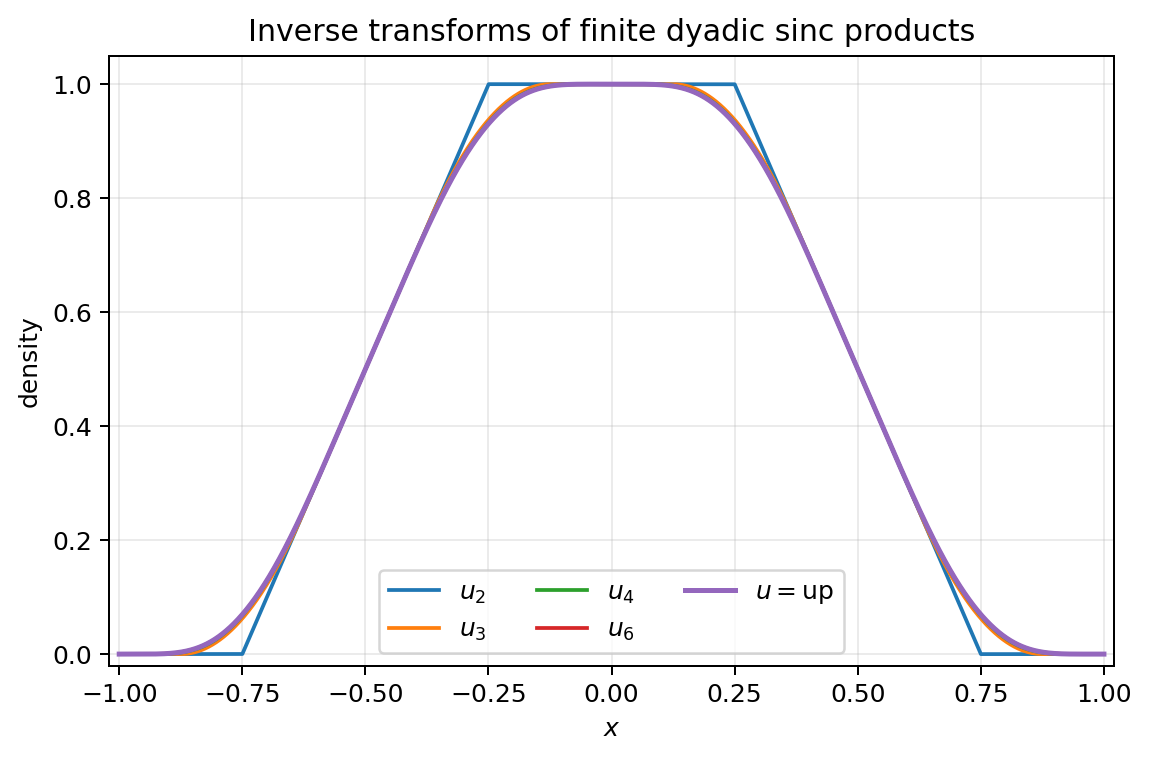
\includegraphics[width=0.91\textwidth]{assets/fabius_finite_products_frontier/figures/finite_spline_approximants.png}
\caption{The inverse transforms $u_N$ are nonnegative degree-$N-1$ splines with support $[-1+2^{-N},1-2^{-N}]$ and plateau $[-2^{-N},2^{-N}]$.  Their geometric convergence is already visually rapid.}
\label{p5:fig:approximants}
\end{figure}

\begin{figure}[htbp]
\centering
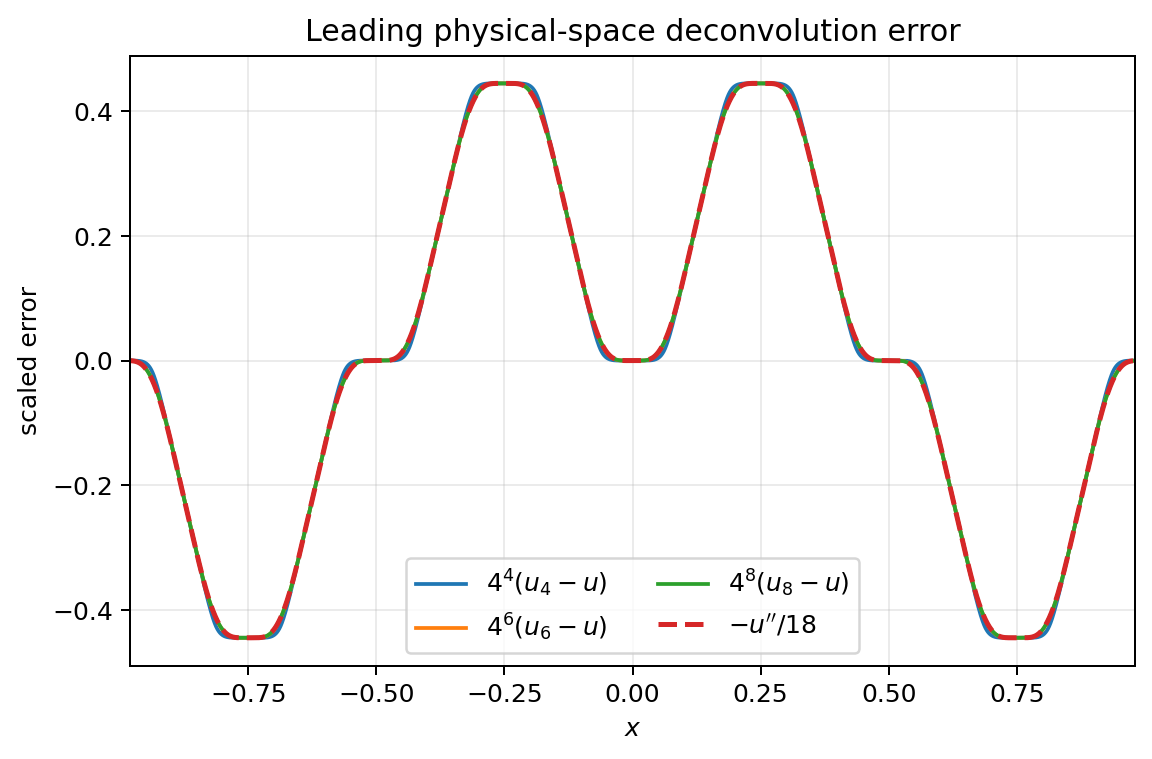
\includegraphics[width=0.91\textwidth]{assets/fabius_finite_products_frontier/figures/scaled_density_error.png}
\caption{The scaled errors $4^N(u_N-u)$ collapse onto the baseline limit $-u''/18$.  The zero pattern at $0$ and $\pm1/2$ is exact at every stage.}
\label{p5:fig:density-error}
\end{figure}

\begin{figure}[htbp]
\centering
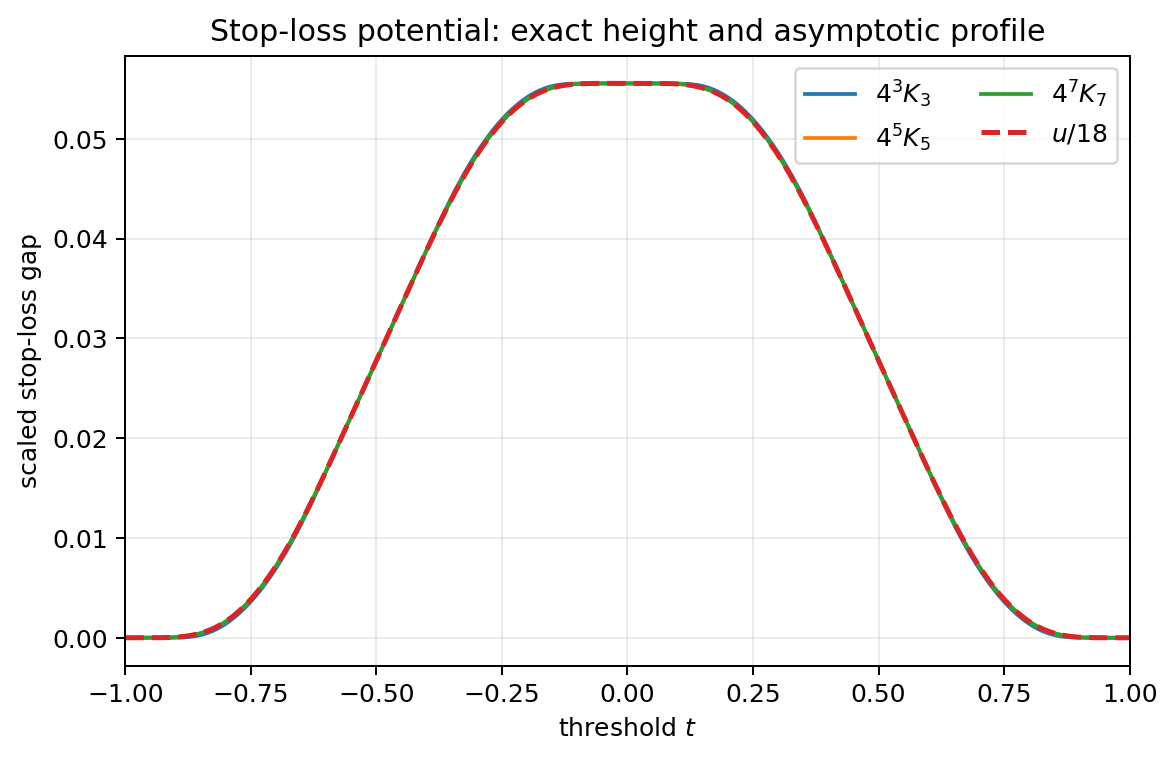
\includegraphics[width=0.91\textwidth]{assets/fabius_finite_products_frontier/figures/scaled_stop_loss.png}
\caption{The exact call-potential gaps satisfy $K_N(0)=4^{-N}/18$ and converge after scaling to $u/18$.  The central flatness is inherited from the up-function.}
\label{p5:fig:stoploss}
\end{figure}

\subsection{Exact metric checks}

\begin{table}[htbp]
\centering
\small
\caption{FFT verification of two representative exact identities.  The table uses $M=2^{18}$ period-two samples.}
\label{p5:tab:metric-check}
\setlength{\tabcolsep}{4pt}% ed.: tightened so the seven columns fit
\begin{tabular}{@{}rcccccc@{}}
\toprule
$N$ & $W_1$ numeric & $W_1$ exact & rel. error & $\max K_N$ numeric & exact & rel. error\\
\midrule
2 & $6.944444\times10^{-3}$ & $6.944444\times10^{-3}$ & $2.82e-10$ & $3.472222\times10^{-3}$ & $3.472222\times10^{-3}$ & $1.86e-10$ \\
3 & $1.736111\times10^{-3}$ & $1.736111\times10^{-3}$ & $2.85e-11$ & $8.680556\times10^{-4}$ & $8.680556\times10^{-4}$ & $1.63e-12$ \\
4 & $4.340278\times10^{-4}$ & $4.340278\times10^{-4}$ & $5.68e-10$ & $2.170139\times10^{-4}$ & $2.170139\times10^{-4}$ & $8.65e-12$ \\
5 & $1.085069\times10^{-4}$ & $1.085069\times10^{-4}$ & $1.83e-09$ & $5.425347\times10^{-5}$ & $5.425347\times10^{-5}$ & $9.21e-11$ \\
6 & $2.712674\times10^{-5}$ & $2.712674\times10^{-5}$ & $1.82e-09$ & $1.356337\times10^{-5}$ & $1.356337\times10^{-5}$ & $1.04e-10$ \\
7 & $6.781684\times10^{-6}$ & $6.781684\times10^{-6}$ & $1.42e-10$ & $3.390842\times10^{-6}$ & $3.390842\times10^{-6}$ & $3.21e-10$ \\
8 & $1.695421\times10^{-6}$ & $1.695421\times10^{-6}$ & $5.80e-08$ & $8.477105\times10^{-7}$ & $8.477105\times10^{-7}$ & $5.12e-09$ \\
9 & $4.238552\times10^{-7}$ & $4.238553\times10^{-7}$ & $1.15e-07$ & $2.119276\times10^{-7}$ & $2.119276\times10^{-7}$ & $2.77e-09$ \\
10 & $1.059638\times10^{-7}$ & $1.059638\times10^{-7}$ & $2.17e-07$ & $5.298191\times10^{-8}$ & $5.298191\times10^{-8}$ & $1.10e-08$ \\
\bottomrule
\end{tabular}
\end{table}

The largest relative error in the tabulated $W_1$ values is $2.2\times10^{-7}$, occurring at the smallest absolute value $N=10$; the largest stop-loss relative error is $1.1\times10^{-8}$.  The same run numerically returns
\begin{equation}
 \int u=1,
 \qquad
 \int\abs{u'}=2,
 \qquad
 \int\abs{u''}=8
 \label{p5:eq:diagnostics}
\end{equation}
to double precision.  The last identity also follows analytically from $u'(1/2)=-2u(0)=-2$ and the sign pattern of $u''$.

\begin{figure}[htbp]
\centering
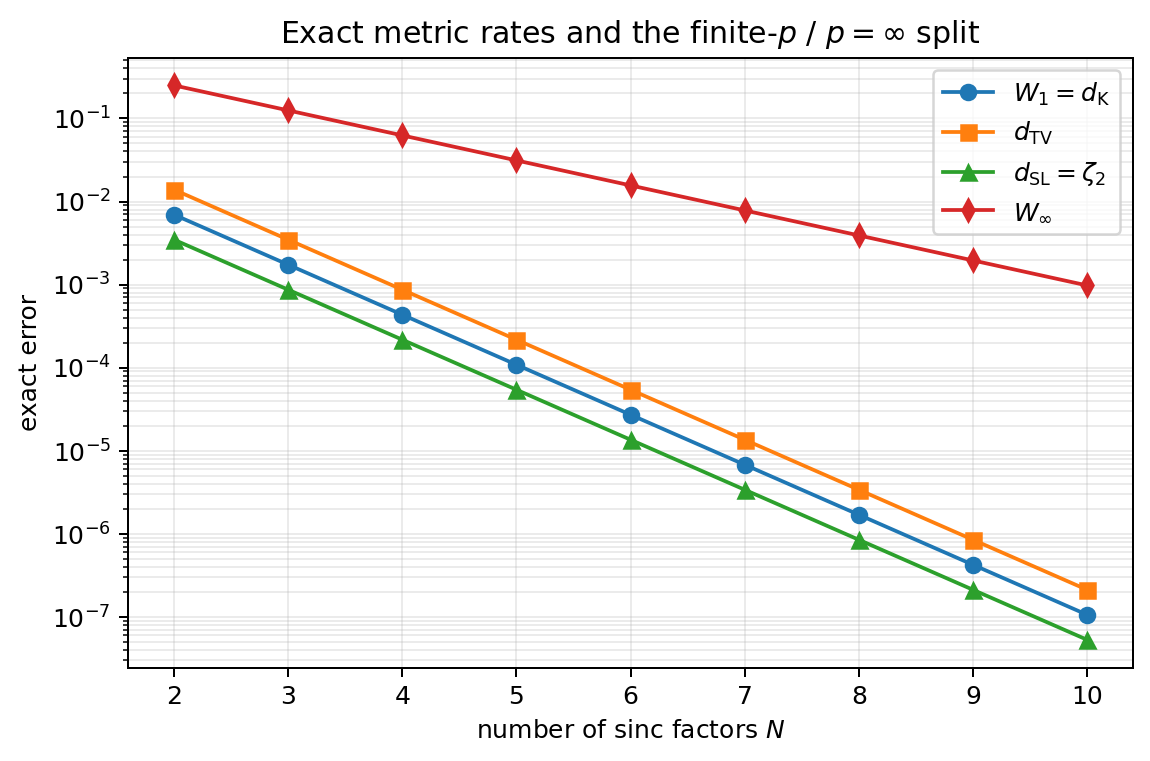
\includegraphics[width=0.88\textwidth]{assets/fabius_finite_products_frontier/figures/exact_metric_rates.png}
\caption{The finite metrics have exact $4^{-N}$ rates, whereas $W_\infty$ has exact rate $2^{-N}$.  This is the first indication of the finite-$p$/$p=\infty$ crossover.}
\label{p5:fig:metric-rates}
\end{figure}

\section{Information geometry and finite-order transport frontiers}
\label{p5:sec:information}

This section separates rigorous monotonicity statements from asymptotic conjectures requiring endpoint-weighted remainder control.

\subsection{Entropy monotonicity and convergence}

For a density $f$, write
\[
 \Ent(f)=-\int f\log f,
 \qquad
 \Fish(f)=\int\frac{(f')^2}{f},
\]
with the usual conventions.

\begin{theorem}[Entropy chain; \newresult]
The sequence $\Ent(u_N)$ is strictly increasing and
\begin{equation}
 \Ent(u_N)\uparrow\Ent(u).
 \label{p5:eq:entropy-chain}
\end{equation}
\end{theorem}

\begin{proof}
Since $X_{N+1}=X_N+2^{-(N+1)}V_{N+1}$ with an independent nondegenerate summand, the entropy-power inequality gives $\Ent(u_{N+1})>\Ent(u_N)$.  The densities converge in $L^1$, are supported in $[-1,1]$, and satisfy $0\le u_N\le1$ because $u_N$ is a convolution of the unit-height first box with a probability density.  The continuous function $-x\log x$ on $[0,1]$ is uniformly bounded, so convergence in measure plus dominated convergence yields $\Ent(u_N)\to\Ent(u)$.
\end{proof}

\begin{proposition}[Asymmetric relative entropy; \newresult]
For every finite $N$,
\begin{equation}
 \KL(u\Vert u_N)=+\infty,
 \qquad
 \KL(u_N\Vert u)<\infty.
 \label{p5:eq:KL-asymmetry}
\end{equation}
\end{proposition}

\begin{proof}
The limiting density is strictly positive on $(-1,1)$, while $u_N$ vanishes on the two strips $a_N<\abs x<1$ of positive $u$-mass.  Hence the reverse logarithmic ratio is infinite there.  In the forward direction, $u$ is positive on the compact interior support of $u_N$, and the polynomial vanishing of $u_N$ at its own endpoints makes $u_N\log(u_N/u)$ integrable.
\end{proof}

\subsection{Fisher information}

Near a support endpoint, the spline formula gives
\begin{equation}
 u_N(a_N-y)\asymp y^{N-1},
 \qquad
 u_N'(a_N-y)\asymp y^{N-2}.
 \label{p5:eq:endpoint-power}
\end{equation}
Therefore $(u_N')^2/u_N\asymp y^{N-3}$.

\begin{theorem}[Finite-stage Fisher criterion and monotonicity; \newresult]
\begin{equation}
 \Fish(u_N)<\infty\quad\Longleftrightarrow\quad N\ge3.
 \label{p5:eq:fisher-criterion}
\end{equation}
For $N\ge3$,
\begin{equation}
 \Fish(u_{N+1})\le\Fish(u_N).
 \label{p5:eq:fisher-monotone}
\end{equation}
Moreover $\Fish(u)\le\lim_{N\to\infty}\Fish(u_N)$.
\end{theorem}

\begin{proof}
The integrability criterion follows from \eqref{p5:eq:endpoint-power}.  For monotonicity, the score of a convolution is the conditional expectation of the score of the first summand given the sum.  Conditional Jensen therefore decreases its squared $L^2$ norm.  The final inequality is lower semicontinuity of Fisher information under weak convergence.
\end{proof}

Equality of the limit with $\Fish(u)$ is strongly supported numerically and is included in the conjecture below.

\subsection{Weighted information asymptotics}

Set
\begin{equation}
 I=\Fish(u)=\int_{-1}^{1}\frac{u'(x)^2}{u(x)}\dd x,
 \qquad
 J=\int_{-1}^{1}\frac{u''(x)^2}{u(x)}\dd x,
 \label{p5:eq:I-J}
\end{equation}
and
\begin{equation}
 L=\int_{-1}^{1}u(x)\left((\log u(x))''\right)^2\dd x.
 \label{p5:eq:L-info}
\end{equation}
The FFT computation gives
\begin{equation}
\begin{gathered}
 \Ent(u)\approx0.297039912826071,
 \qquad I\approx11.8007105434191,\\
 J\approx1619.745753585,
 \qquad L\approx485.548634253.
\end{gathered}
 \label{p5:eq:numeric-info-constants}
\end{equation}

\begin{conjecture}[Information expansion]
As $N\to\infty$,
\begin{align}
 \Ent(u)-\Ent(u_N)
 &=\frac{4^{-N}}{18}I+\bigO(16^{-N}),
 \label{p5:eq:entropy-conj}\\
 \KL(u_N\Vert u)
 &=\frac{16^{-N}}{648}J+\bigO(64^{-N}),
 \label{p5:eq:KL-conj}\\
 \Fish(u_N)
 &=\Fish(u)+\frac{4^{-N}}9L+\bigO(16^{-N}).
 \label{p5:eq:fisher-conj}
\end{align}
In particular, $\Fish(u_N)\downarrow\Fish(u)$.
\end{conjecture}

\begin{proofidea}
Formally insert
\[
 u_N=u-\frac{\eps_N^2}{18}u''+\bigO(\eps_N^4)
\]
into the entropy, relative-entropy, and Fisher functionals.  The first variations give \eqref{p5:eq:entropy-conj}; the quadratic term of KL gives \eqref{p5:eq:KL-conj}.  For Fisher information, one integration-by-parts reduction turns the first variation into
\[
 \frac{\eps_N^2}{9}\int u((\log u)'')^2.
\]
The missing rigorous step is a version of \eqref{p5:eq:physical-expansion} in weighted spaces containing inverse powers of $u$.  Uniform $C^r$ control alone is insufficient because $u$ is flat at $\pm1$.  The repository's lower-Lambert endpoint expansion appears strong enough to supply the needed split-domain domination.
\end{proofidea}

\subsection{Fixed-order Wasserstein asymptotics}

For $1\le p<\infty$, define the score moment
\begin{equation}
 J_p=\int_{-1}^{1}\abs{u'(x)}^p u(x)^{1-p}\dd x
 =\int_0^1\abs{(\log u)'(Q(s))}^p\dd s.
 \label{p5:eq:Jp}
\end{equation}
Flatness makes $J_p$ finite for each fixed $p$, although $J_p^{1/p}\to\infty$ as $p\to\infty$.

\begin{conjecture}[Finite-$p$ transport law]
For every fixed $1\le p<\infty$,
\begin{equation}
 \boxed{
 W_p(\mu_N,\mu)
 \sim\frac{4^{-N}}{18}J_p^{1/p}.}
 \label{p5:eq:Wp-conj}
\end{equation}
For $p=1$, this is the proved exact formula because $J_1=\int\abs{u'}=2$.  For $p=2$,
\begin{equation}
 W_2(\mu_N,\mu)
 \sim\frac{4^{-N}}{18}\sqrt{\Fish(u)}.
 \label{p5:eq:W2-conj}
\end{equation}
\end{conjecture}

\begin{proofidea}
The interior quantile expansion \eqref{p5:eq:quantile-leading} gives
\[
 \abs{Q_N(s)-Q(s)}^p
 \sim\left(\frac{4^{-N}}{18}\right)^p
 \abs{(\log u)'(Q(s))}^p.
\]
Integrating over $s$ gives \eqref{p5:eq:Wp-conj}.  The endpoint layers must again be controlled with the lower-Lambert expansion; fixed $p$ should make their contribution negligible at the $4^{-Np}$ scale.
\end{proofidea}

\begin{figure}[htbp]
\centering
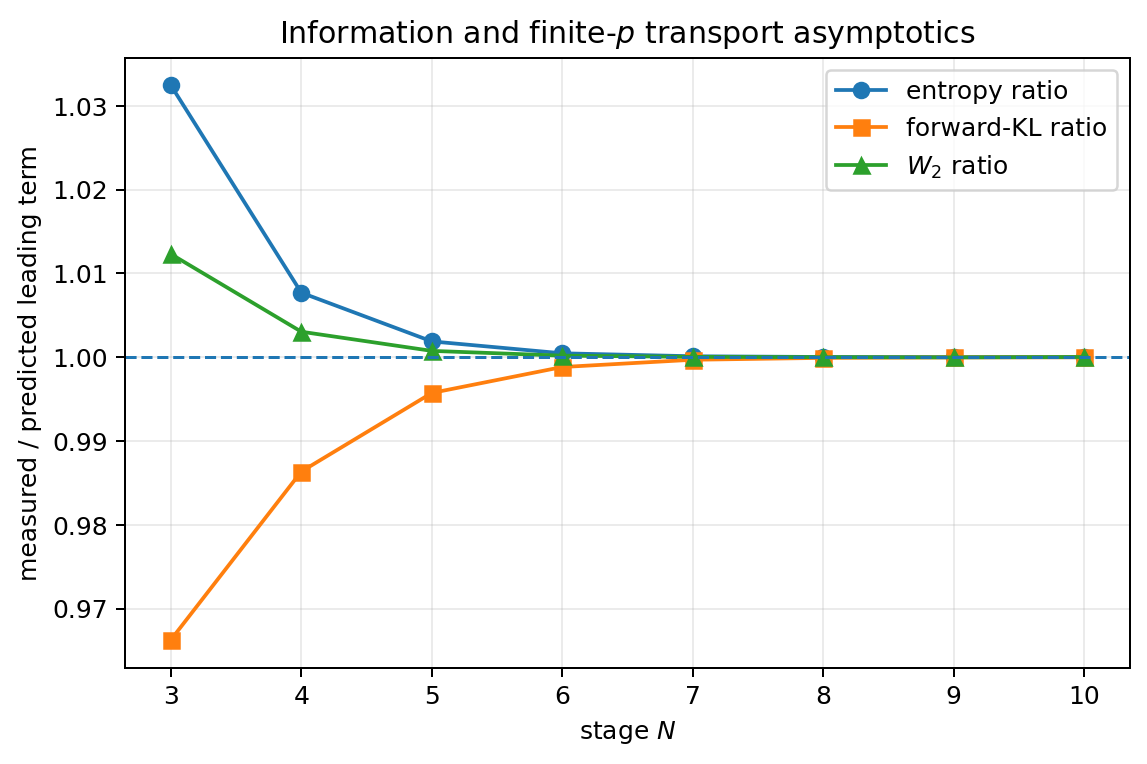
\includegraphics[width=0.88\textwidth]{assets/fabius_finite_products_frontier/figures/information_transport_ratios.png}
\caption{Measured values divided by the predicted leading terms in \eqref{p5:eq:entropy-conj}, \eqref{p5:eq:KL-conj}, and \eqref{p5:eq:W2-conj}.  All ratios approach one rapidly.}
\label{p5:fig:info-ratios}
\end{figure}

\begin{table}[htbp]
\centering
\small
\caption{Numerical evidence for the information and $W_2$ conjectures.  ``Ratio'' means measured value divided by the displayed leading asymptotic term.}
\label{p5:tab:information}
\begin{tabular}{@{}rcccccc@{}}
\toprule
$N$ & entropy gap & ratio & $D(u_N\Vert u)$ & ratio & $W_2$ & ratio\\
\midrule
3 & $1.057601\times10^{-2}$ & $1.03244285$ & $5.896794\times10^{-4}$ & $0.96628234$ & $3.018666\times10^{-3}$ & $1.01230978$ \\
4 & $2.580642\times10^{-3}$ & $1.00770183$ & $3.762085\times10^{-5}$ & $0.98636290$ & $7.477592\times10^{-4}$ & $1.00304444$ \\
5 & $6.414394\times10^{-4}$ & $1.00188982$ & $2.373649\times10^{-6}$ & $0.99573677$ & $1.865139\times10^{-4}$ & $1.00075897$ \\
6 & $1.601326\times10^{-4}$ & $1.00046967$ & $1.488143\times10^{-7}$ & $0.99883278$ & $4.660192\times10^{-5}$ & $1.00018926$ \\
7 & $4.001904\times10^{-5}$ & $1.00011722$ & $9.308961\times10^{-9}$ & $0.99969898$ & $1.164881\times10^{-5}$ & $1.00004596$ \\
8 & $1.000388\times10^{-5}$ & $1.00002929$ & $5.819411\times10^{-10}$ & $0.99992405$ & $2.912086\times10^{-6}$ & $1.00000594$ \\
9 & $2.500915\times10^{-6}$ & $1.00000732$ & $3.637339\times10^{-11}$ & $0.99998105$ & $7.280062\times10^{-7}$ & $0.99998492$ \\
10 & $6.252253\times10^{-7}$ & $1.00000183$ & $2.273371\times10^{-12}$ & $0.99999627$ & $1.820097\times10^{-7}$ & $1.00002973$ \\
\bottomrule
\end{tabular}
\end{table}

\begin{figure}[htbp]
\centering
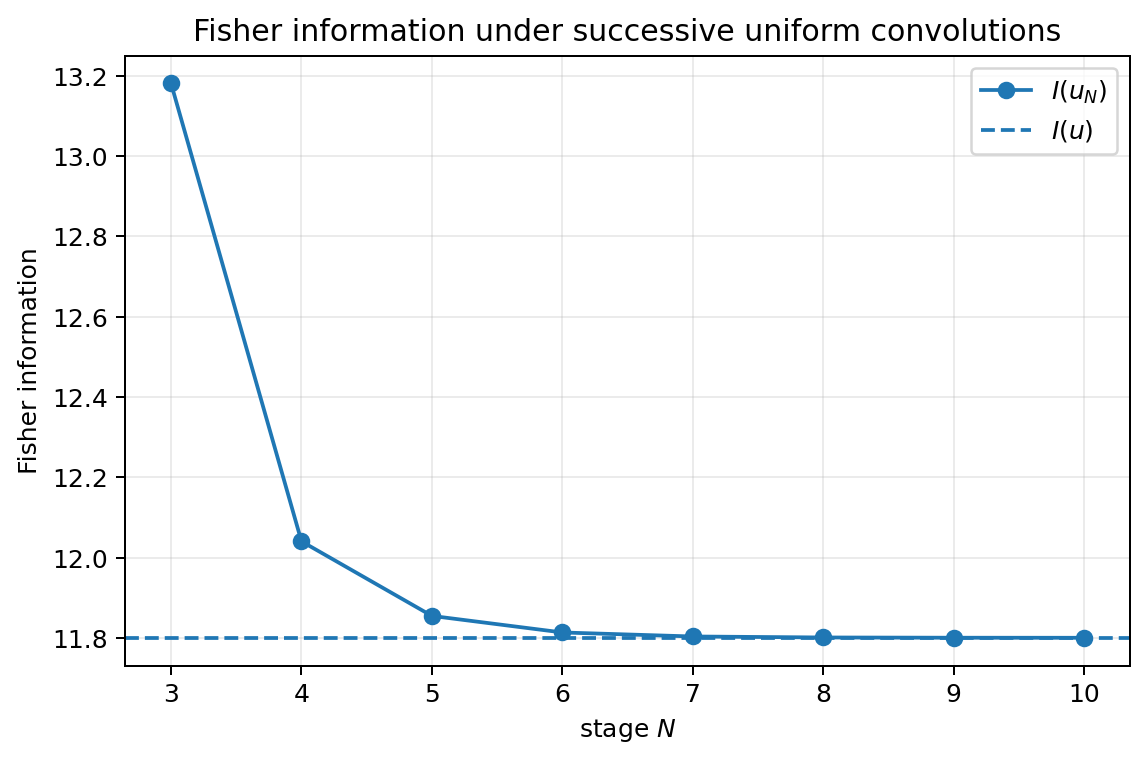
\includegraphics[width=0.86\textwidth]{assets/fabius_finite_products_frontier/figures/fisher_information.png}
\caption{Numerical monotone convergence of $\Fish(u_N)$ to $\Fish(u)\approx11.8007105434191$.  The measured first correction agrees with $4^{-N}L/9$.}
\label{p5:fig:fisher}
\end{figure}

\subsection{The transport-order crossover near twice the truncation stage}

The exact endpoint result $W_\infty=2^{-N}$ cannot be obtained by sending $p\to\infty$ after taking the fixed-$p$ asymptotic.  The lower-Lambert endpoint law suggests
\begin{equation}
 J_p^{1/p}=2^{p/2}\,p^{\theta+\smallo(1)}
 \times\bigl(\text{bounded log-periodic factor}\bigr)
 \label{p5:eq:Jp-growth}
\end{equation}
for a computable exponent $\theta$.  Balancing
\[
 4^{-N}J_p^{1/p}\asymp2^{-N}
\]
then places the transition near
\begin{equation}
 p=2N+\bigO(\log N).
 \label{p5:eq:crossover}
\end{equation}

\begin{conjecture}[Double-scaling transport crossover]
There is a nontrivial profile $\mathcal W(\lambda,\vartheta)$ such that, with
$p=2N+\lambda\log N+\bigO(1)$ and with $\vartheta$ the dyadic lower-Lambert phase,
\begin{equation}
 2^N W_p(\mu_N,\mu)\longrightarrow\mathcal W(\lambda,\vartheta)
 \label{p5:eq:crossover-profile}
\end{equation}
along phase-locked subsequences.  The profile interpolates between the score-moment regime and the endpoint value one.
\end{conjecture}

The periodic phase is not cosmetic: the repository's endpoint theory proves that it is nonconstant.  Any crossover theorem that averages it away prematurely is likely to miss subsequential structure.

\section{Further deductions and research directions}
\label{p5:sec:future}

\subsection{Weighted endpoint remainder theorem}

The most immediate target is a theorem of the schematic form
\begin{equation}
 \int_{-1}^{1}
 \frac{\abs{u_N-u+\eps_N^2u''/18}^q}{u^{q-1}}
 \dd x
 =\bigO(\eps_N^{4q})
 \label{p5:eq:weighted-remainder-goal}
\end{equation}
for suitable $q$, together with derivative analogues.  A proof should split the interval in the exact lower-Lambert coordinate, use the periodic endpoint transseries in the boundary layer, and use the ordinary $C^r$ expansion in the bulk.  This single technical result would rigorously settle \eqref{p5:eq:entropy-conj}, \eqref{p5:eq:KL-conj}, and fixed-$p$ cases of \eqref{p5:eq:Wp-conj}.

\subsection{Exact Wasserstein values beyond first order}

The one-dimensional optimal coupling is monotone, so
\begin{equation}
 W_p^p(\mu_N,\mu)=\int_0^1\abs{Q_N(s)-Q(s)}^p\dd s.
 \label{p5:eq:Wp-quantile}
\end{equation}
The exact dyadic arithmetic of $H_N$ and the inverse-Fabius infrastructure suggest several possibilities:

\begin{enumerate}
\item exact recurrences or rapidly convergent series for $W_2^2$;
\item arithmetic information about quadrature approximants to \eqref{p5:eq:Wp-quantile};
\item bounds obtained from the exact call potential and one-dimensional Sobolev inequalities;
\item phase-locked asymptotics for $p$ growing with $N$.
\end{enumerate}

\subsection{Total positivity and variation diminution}

Every finite approximant is a convolution of boxes, hence belongs to the classical P\'olya-frequency/spline setting of Curry and Schoenberg \cite{p5:CurrySchoenberg1966}.  The fixed density crossing suggests a stronger variation-diminishing statement for the deconvolution chain:

\begin{conjecture}[Higher derivative crossing hierarchy]
For each fixed $r$, the error $u_N^{(r)}-u^{(r)}$ has, for all sufficiently large $N$, the same number and ordering of sign changes as $-u^{(r+2)}$, and the zeros converge with complete $4^{-N}$ expansions.  At special dyadic zeros forced by flatness, some crossings are exact at every stage.
\end{conjecture}

Such a theorem would turn the all-orders $C^r$ expansion into exact shape information and could yield closed formulas for additional $L^1$ derivative norms.

\subsection{Nonlinear positive acceleration}

The positive-mixture theorem rules out linear convex acceleration, but not nonlinear transformations that preserve nonnegativity and mass.  Promising candidates include:

\begin{enumerate}
\item exponentiating a Richardson combination of logarithmic characteristic-function tails and then proving positive definiteness;
\item monotone transport extrapolation at the quantile level;
\item entropy projection of a signed Richardson density onto the convex set of probability densities with prescribed moments;
\item call-potential extrapolation followed by projection onto the cone of nonnegative convex-order gaps.
\end{enumerate}

Any such method must respect the exact support deficit, the fixed crossing at $1/2$, and the zero divisor of the finite Fourier product.

\subsection{Formalization roadmap}

The most Lean-friendly new results are elementary once the probability model is available:

\begin{enumerate}
\item the conditional formula \eqref{p5:eq:uniform-absolute};
\item the exact absolute moment \eqref{p5:eq:absolute-moments};
\item peakedness from one-dimensional interval rearrangement;
\item the error identity \eqref{p5:eq:error-cdf-identity} and single crossing;
\item exact $W_1$, Kolmogorov, and TV constants;
\item the call spline \eqref{p5:eq:put-spline};
\item exact potential height/area and the positive-mixture no-go theorem.
\end{enumerate}

The information conjectures should wait until the weighted endpoint calculus is formalized.  The exact metric package, by contrast, uses only finite sums, conditioning, symmetry, monotonicity, and elementary integration.

\section{Compact theorem and formula index}
\label{p5:sec:index}

\begin{longtable}{@{}p{0.29\textwidth}p{0.61\textwidth}@{}}
\toprule
Object & Formula or property\\
\midrule
\endfirsthead
\toprule
Object & Formula or property\\
\midrule
\endhead
Finite product & $\Phi_N(\xi)=\prod_{j=1}^{N}\sinc(\xi/2^j)$.\\
Random variable & $X_N=\sum_{j=1}^{N}2^{-j}V_j$, $V_j\sim\operatorname{Unif}[-1,1]$.\\
Tail & $X=X_N+2^{-N}X'$, $\Phi=\Phi_N\Phi(2^{-N}\cdot)$.\\
Support/plateau & $\supp u_N=[-1+2^{-N},1-2^{-N}]$, $u_N=1$ on $[-2^{-N},2^{-N}]$.\\
Knots & $\kappa_{N,m}=-1+(2m+1)/2^N$.\\
Spline & Equation \eqref{p5:eq:spline-formula}; degree $N-1$, smoothness $C^{N-2}$.\\
Leading density error & $4^N(u_N-u)\to-u''/18$.\\
Convex order & $\mu_N\preceq_{\rm cx}\mu_{N+1}\preceq_{\rm cx}\mu$.\\
Absolute moment & $\E\abs{X_N}=5/18-4^{-N}/9$.\\
Single crossing & $u_N-u>0$ for $0<\abs x<1/2$, negative for $1/2<\abs x<1$.\\
$W_1$ & $4^{-N}/9$ for all $N\ge1$.\\
Kolmogorov & $4^{-N}/9$ for $N\ge2$; $5/72$ for $N=1$.\\
Total variation & $2\,4^{-N}/9$ for $N\ge2$; $5/36$ for $N=1$.\\
$W_\infty$ & $2^{-N}$.\\
Call potential & $K_N=C-C_N\ge0$, exact finite spline from \eqref{p5:eq:put-spline}.\\
Stop-loss/Zolotarev & Both equal $4^{-N}/18$.\\
Potential profile & $4^NK_N\to u/18$ in every $C^r$.\\
Positive mixture & Every finite metric is multiplied by $A(\alpha)=\sum\alpha_j4^{-j}$; no cancellation.\\
Entropy & $\Ent(u_N)\uparrow\Ent(u)$.\\
Reverse KL & $\KL(u\Vert u_N)=\infty$.\\
Fisher & Finite iff $N\ge3$; nonincreasing thereafter.\\
Conjectured $W_p$ & $W_p\sim4^{-N}J_p^{1/p}/18$ for fixed finite $p$.\\
\bottomrule
\end{longtable}

\appendix

\section{The first-stage exception in detail}
\label{p5:app:first}

The first approximant is
\[
 u_1=\mathbf1_{[-1/2,1/2]}.
\]
The CDF difference still has one positive maximum at $1/2$, but the reduction through $X_{N-1}$ would require the degenerate stage $X_0=0$.  Directly,
\[
 d_1(1/2)=H_1(1/2)-H(1/2)
 =1-\left(1-\frac14\E\abs X\right)
 =\frac5{72}.
\]
The density crossing then gives
\[
 \norm{u_1-u}_1=4d_1(1/2)=\frac5{18}.
\]
By contrast, $W_1$ depends on the absolute-moment difference and remains on the universal formula
\[
 W_1=\E\abs X-\E\abs{X_1}
 =\frac5{18}-\frac14=\frac1{36}.
\]
The stop-loss value also remains universal:
\[
 K_1(0)=\frac12W_1=\frac1{72}.
\]

\section{Derivation of the Fisher first variation}
\label{p5:app:fisher}

Let $f_\eta=u+\eta v$ with $\int v=0$.  The first variation of Fisher information is
\begin{equation}
 \left.\frac{\dd}{\dd\eta}\Fish(f_\eta)\right|_{\eta=0}
 =\int\left(\frac{2u'v'}u-\frac{u'^2v}{u^2}\right)\dd x.
 \label{p5:eq:fisher-variation}
\end{equation}
For the finite-product deconvolution, $v=-u''/18$.  Put $s=(\log u)'$.  Since
\[
 \frac{u''}{u}=s'+s^2,
 \qquad
 \frac{u'''}u=s''+3ss'+s^3,
\]
the bracket before the factor $-1/18$ becomes
\[
 u\left(2ss''+5s^2s'+s^4\right).
\]
Integration by parts gives
\[
 \int2uss''=-2\int u\bigl((s')^2+s^2s'\bigr),
\]
and
\[
 3\int us^2s'=-\int us^4.
\]
The quartic terms cancel, leaving
\[
 \int\left(\frac{2u'(-u''')}{u}+\frac{u'^2u''}{u^2}\right)\dd x
 =2\int u(s')^2\dd x.
\]
Multiplication by $\eps_N^2/18$ therefore yields the conjectured first correction $\eps_N^2L/9$ in \eqref{p5:eq:fisher-conj}.

\section{Reproducibility ledger}
\label{p5:app:repro}

\subsection{Archive contents}

The companion archive contains:

% ed.: first column widened so the long mono paths fit without overfull
\begin{longtable}{@{}p{0.43\textwidth}p{0.49\textwidth}@{}}
\toprule
Path & Purpose\\
\midrule
\texttt{finite\_sinc\_frontier.tex} & Complete source of this report.\\
\texttt{finite\_sinc\_frontier.pdf} & Compiled report.\\
\texttt{finite\_sinc\_experiments.py} & Standalone, fully commented numerical experiment.\\
\texttt{figures/*.pdf} & Vector figures included in the report.\\
\texttt{figures/*.png} & Raster previews of the same figures.\\
\texttt{data/metric\_verification.csv} & Numerical and exact metric values.\\
\texttt{data/information\_transport.csv} & Entropy, KL, Fisher, and $W_2$ data.\\
\texttt{data/reference\_constants.csv} & Computed normalization and information constants.\\
\texttt{data/verification\_log.txt} & Human-readable diagnostics and maximum errors.\\
\texttt{README.md} & Commands and dependency notes.\\
\bottomrule
\end{longtable}

\subsection{Audited source hashes}

The four directly materialized overlap-critical sources had the following SHA-256 hashes at audit time:

\begin{longtable}{@{}p{0.38\textwidth}p{0.54\textwidth}@{}}
\toprule
Source & SHA-256\\
\midrule
\nolinkurl{Fabius_Function_and_Rvachev_Up.tex} & \nolinkurl{c2f203778b1889bff22e4839f369c16e50e9ef45799717f6f1357dc1df3f40d1}\\
\nolinkurl{fabius-frontier-results.tex} & \nolinkurl{32953767492749ce7668a28896e76075ab3ab1f9c42f370c4e31e35638f21857}\\
\nolinkurl{Fabius_Rvachev_Multiresolution_Representations.tex} & \nolinkurl{832c790e8bd247ea1569c7ef1ac09017a9c083d7c8f5ed17d57035e2aa82175c}\\
\nolinkurl{Fabius_Dyadic_q_Connections.tex} & \nolinkurl{81a0a911ac7ab28e12c6b87ccaf76ffccaf32e48f873abff18fb7a2d01bcf3e5}\\
\bottomrule
\end{longtable}

\subsection{Numerical command}

From the report directory, the complete numerical layer is regenerated by
\begin{lstlisting}[style=python]
python finite_sinc_experiments.py --output . --grid-power 18 --max-stage 10
\end{lstlisting}
The PDF is then built with
\begin{lstlisting}[style=python]
latexmk -lualatex -interaction=nonstopmode -halt-on-error finite_sinc_frontier.tex
\end{lstlisting}

\begin{thebibliography}{99}

\bibitem{p5:Anderson1955}
T.~W. Anderson,
\newblock The integral of a symmetric unimodal function over a symmetric convex set and some probability inequalities,
\newblock \emph{Proc. Amer. Math. Soc.} \textbf{6} (1955), 170--176.
\newblock doi:10.1090/S0002-9939-1955-0069229-1.

\bibitem{p5:Arias2017}
J. Arias de Reyna,
\newblock An infinitely differentiable function with compact support: definition and properties,
\newblock arXiv:1702.05442 (2017); English translation of \emph{Rev. Real Acad. Ciencias} \textbf{76} (1982), 21--38.

\bibitem{p5:AriasArithmetic}
J. Arias de Reyna,
\newblock Arithmetic of the Fabius function,
\newblock \emph{Integers} \textbf{18} (2018), A51; arXiv:1702.06487.

\bibitem{p5:deBoor}
C. de Boor,
\newblock \emph{A Practical Guide to Splines}, revised edition,
\newblock Springer, 2001.

\bibitem{p5:CurrySchoenberg1966}
H.~B. Curry and I.~J. Schoenberg,
\newblock On P\'olya frequency functions IV: the fundamental spline functions and their limits,
\newblock \emph{J. Analyse Math.} \textbf{17} (1966), 71--107.
\newblock doi:10.1007/BF02788653.

\bibitem{p5:Fabius1966}
J. Fabius,
\newblock A probabilistic example of a nowhere analytic $C^\infty$-function,
\newblock \emph{Z. Wahrscheinlichkeitstheorie verw. Gebiete} \textbf{5} (1966), 173--174.
\newblock doi:10.1007/BF00536652.

\bibitem{p5:GasperRahman}
G. Gasper and M. Rahman,
\newblock \emph{Basic Hypergeometric Series}, second edition,
\newblock Cambridge University Press, 2004.

\bibitem{p5:JessenWintner1935}
B. Jessen and A. Wintner,
\newblock Distribution functions and the Riemann zeta function,
\newblock \emph{Trans. Amer. Math. Soc.} \textbf{38} (1935), 48--88.
\newblock doi:10.1090/S0002-9947-1935-1501802-5.

\bibitem{p5:ShakedShanthikumar}
M. Shaked and J.~G. Shanthikumar,
\newblock \emph{Stochastic Orders},
\newblock Springer, 2007.

\bibitem{p5:Stam1959}
A.~J. Stam,
\newblock Some inequalities satisfied by the quantities of information of Fisher and Shannon,
\newblock \emph{Information and Control} \textbf{2} (1959), 101--112.
\newblock doi:10.1016/S0019-9958(59)90348-1.

\bibitem{p5:Villani}
C. Villani,
\newblock \emph{Topics in Optimal Transportation},
\newblock Graduate Studies in Mathematics 58, American Mathematical Society, 2003.

\bibitem{p5:Zolotarev}
V.~M. Zolotarev,
\newblock \emph{Modern Theory of Summation of Random Variables},
\newblock VSP, Utrecht, 1997.

\bibitem{p5:ProveItPrimary}
V. Reshetnikov,
\newblock The Fabius function and Rvachev's up-function,
\newblock source in the \texttt{ProveIt} repository, \repo{}, commit \texttt{21758aba2f8e200342be2a7b321247dac80efc00}.

\bibitem{p5:ProveItFrontiers}
V. Reshetnikov et al.,
\newblock Non-formalized research frontiers and thematic draft consolidations for the Fabius--Rvachev system,
\newblock \texttt{ProveIt} repository, \repo{}/\texttt{semi-formalized-research-frontiers}, same commit.

\end{thebibliography}



%% ================= Part VI =================
% Non-duplicate preamble layer for Part VI (theorem environments and
% shared letter macros already provided by the volume; \wt and \vtwo
% render in the volume's convention; \repo re-declared for this
% part).
\definecolor{sourceblue}{RGB}{232,241,250}
\definecolor{repogreen}{RGB}{235,247,239}
\definecolor{newgold}{RGB}{252,247,227}
\definecolor{conjrose}{RGB}{252,236,239}
\newcommand{\Fup}{\operatorname{Fup}}
\newcommand{\Hh}{\widehat h}
\newcommand{\1}{\mathbf 1}
\newcommand{\dist}{\operatorname{dist}}
\newcommand{\diam}{\operatorname{diam}}
\newcommand{\LipVI}{\operatorname{Lip}}
\newcommand{\DF}{D_{\!F}}
\newcommand{\sourceflag}{\textsf{[S]}}
\newcommand{\repoflag}{\textsf{[R]}}
\newcommand{\newflag}{\textsf{[N]}}
\newcommand{\conjflag}{\textsf{[C]}}
\renewcommand{\repo}{\nolinkurl{Analysis/FabiusFunction}}
\newtcolorbox{scopebox}{
  enhanced,breakable,colback=shadegray,colframe=rulegray,
  boxrule=0.5pt,arc=0pt,left=7pt,right=7pt,top=6pt,bottom=6pt
}
\newtcolorbox{sourcebox}{
  enhanced,breakable,colback=sourceblue,colframe=linkblue,
  boxrule=0.6pt,arc=0pt,left=7pt,right=7pt,top=6pt,bottom=6pt,
  title={\sourceflag\ Source translation or source reconstruction},fonttitle=\bfseries
}
\newtcolorbox{repobox}{
  enhanced,breakable,colback=repogreen,colframe=rulegray,
  boxrule=0.6pt,arc=0pt,left=7pt,right=7pt,top=6pt,bottom=6pt,
  title={\repoflag\ Repository baseline or crosswalk},fonttitle=\bfseries
}
\newtcolorbox{novelbox}{
  enhanced,breakable,colback=newgold,colframe=rulegray,
  boxrule=0.6pt,arc=0pt,left=7pt,right=7pt,top=6pt,bottom=6pt,
  title={\newflag\ Repository-relative new derivation},fonttitle=\bfseries
}
\newtcolorbox{conjbox}{
  enhanced,breakable,colback=conjrose,colframe=rulegray,
  boxrule=0.6pt,arc=0pt,left=7pt,right=7pt,top=6pt,bottom=6pt,
  title={\conjflag\ Conjectural or programmatic statement},fonttitle=\bfseries
}
\lstdefinestyle{repoPython}{
  language=Python,
  basicstyle=\ttfamily\small,
  backgroundcolor=\color{shadegray},
  frame=single,
  rulecolor=\color{rulegray},
  columns=fullflexible,
  keepspaces=true,
  showstringspaces=false,
  xleftmargin=0.7em,
  xrightmargin=0.7em,
  aboveskip=0.8em,
  belowskip=0.8em,
  breaklines=true
}
% ed.: restore arabic section numbering after Part V
\setcounter{section}{0}
\renewcommand{\thesection}{\arabic{section}}
\part{Atomic Sinc-Product Splines Beyond the Binary Point}
% Absorbed from atomic_sinc_splines_report_package/atomic_sinc_splines_report.tex (thirteenth wave): an English
% translation and frontier expansion of Rvachev's Chapter 3 on the
% geometric family h_a.
% Merged editorially with Atomic_Functions_Beyond_Dyadic_Report/ (fourteenth wave),
% a second independent reconstruction of the same chapter; its new layers
% (fractal strings/tube formula, degree law, parameter limits, general-base
% Gamma-zeta Laplace decomposition, Fup ladder) appear as dedicated sections,
% and its shared translation/h_a core is deduplicated against this part.
% Also merged with Rvachev_Atomic_Functions_Report/ (fifteenth wave), a third
% independent reconstruction; its new layers (signed gap leading coefficients,
% derivative equimeasurability + all-p norms, the classical Fup_n hierarchy
% with triangular reconstruction and CLT, edge pantograph equations) likewise
% appear as dedicated material, with the shared core deduplicated.

\begin{abstract}
The attached Russian chapter develops \emph{atomic functions}: compactly supported
solutions of differential--functional equations, with Rvachev's function
$\Up$ as the principal example.  This report supplies a mathematically edited
English translation of the chapter's surviving material and expands it in the
notation of the current \repo\ documentation.  The central family is
\[
  \widehat h_a(\xi)=\prod_{j\ge 1}\sinc(2\pi a^{-j}\xi),\qquad a>1,
\]
where $\sinc z=\sin z/z$.  It interpolates between the critical binary atom
$h_2=\Up$ and, for $a>2$, a class of $C^\infty$ functions that are locally
polynomial off a Cantor-type exceptional set.

The translation is followed by a repository-wide crosswalk and several
extensions.  We derive the complete Bernoulli--cumulant and Bell-polynomial
moment calculus for $h_a$; a weighted Prouhet identity giving the entire
derivative hierarchy; exact derivative norms for every $a\ge2$; a finite
truncated-power formula and a self-similar polynomial-gap atlas; a symbolic
localization formula for derivatives on the exceptional set; a rational-power
Strang--Fix theorem that reproduces arbitrary polynomials by one uniform lattice
of shifts whenever some positive power of $a$ is rational; an elementary
log-Gaussian Fourier envelope; and an all-orders asymptotic expansion for the
ordinary finite sinc-product splines.  The leading correction is
\[
 a^{2N}\bigl(h_{a,N}-h_a\bigr)
 \longrightarrow -\frac{h_a''}{6(a^2-1)}
 \quad\text{in every fixed }C^r\text{ norm}.
\]
A deterministic Python program checks the exact moment and Prouhet identities,
computes Fourier inversions without Monte Carlo sampling, and reproduces all
figures and tables in the package.  Claims not yet formalized in Lean are kept
outside the repository's trusted theorem boundary and are labeled accordingly.

This part also absorbs two further independent reconstructions of the same
chapter (fourteenth and fifteenth waves).  Their distinctive layers are folded
in below.  From the fourteenth wave: the complete fractal-string geometry of
the exceptional set for $a>2$ (geometric zeta function, lattice of complex
dimensions, an exact tube formula with nonconstant logarithmic oscillation, and
Minkowski non-measurability); the local polynomial degree as a geometric random
variable, with an exponential scaling limit as $a\downarrow2$; quantitative
Gaussian ($a\downarrow1$) and uniform ($a\to\infty$) parameter limits; an
exact arbitrary-base negative-Laplace decomposition whose one-periodic
correction has Gamma--zeta Fourier modes
$-\Gamma(-\chi_k)\zeta(1-\chi_k)/\log a$; and a canonical $\Fup$ ladder
extending the source's surviving $\Fup_1$ construction.  From the fifteenth
wave: signed closed forms for the leading coefficient on every polynomial gap;
a derivative equimeasurability theorem giving the complete value distribution
and all $L^p$ norms of every derivative for $a>2$; the classical
$\Fup_n$ hierarchy with an exact triangular dyadic averaging reconstruction of
$\Up$ and a quantitative central-limit regime; and the edge pantograph
equations that make the Lambert-$W$ structure of the endpoint visible already
at the level of the differential--functional equation.  Two revised
fourteenth-wave editions add the spectral Stieltjes--Wigert bridge (the
Fourier energy of every $h_a$ realizes the scaled Stieltjes--Wigert moments
$a^{n(n+2)}/2^n$, a non-lognormal representing measure with closed Hankel
determinants and orthogonal polynomials), the Mellin law of the distance to
$K_a$ with its shifted complex-dimension poles, and --- for provenance ---
the Russian source scan and OCR themselves, archived under
\path{assets/}.
\end{abstract}

\begin{scopebox}
\textbf{Status legend and novelty convention.}
\sourceflag\ denotes material translated or reconstructed from the attached
Russian source; \repoflag\ denotes facts already present in the living
repository documentation or its formalization crosswalk; \newflag\ denotes a
derivation that appears new relative to the audited repository corpus, not a
claim of worldwide priority; and \conjflag\ denotes a conjecture, heuristic, or
future research program.  Numerical agreement is evidence only, never a
substitute for proof.
\end{scopebox}

\begin{scopebox}
\textbf{Source condition.}
The supplied \texttt{rvachev.tex} is a 1,267-line OCR transcription containing
the full Chapter 3 through equation (3.100), where Section 5 stops in midstream.
The supplied PDF contains only eleven printed pages, 116--126, beginning in the
middle of Section 2.  The OCR has predictable defects: lost superscripts,
confused Latin and Cyrillic glyphs, corrupted binomial coefficients, equation
numbers such as ``(8.85)'', and occasional reversed Fourier signs.  Whenever the
PDF image resolves a formula, it is preferred.  Otherwise the reconstruction is
checked against adjacent identities, normalization, and the source's own proof.
No text is silently completed beyond the surviving endpoint of Section 5.

The fourteenth- and fifteenth-wave packages reconstructed the same OCR and
page images independently and reached the same readings on every equation the
editions transcribe in common, including the damaged ranges (3.51)--(3.58) and
(3.73)--(3.75), for which all editions record the invariant content (finite
moment reduction at cylinder endpoints; the bit-recursive evaluator with
remainder at most $\Up(-1+2^{-N})$) rather than a fabricated literal
transcription.  The fifteenth wave additionally repairs the endpoint indexing
of (3.51)--(3.58) into an explicit binary-encoded form.  The packages'
OCR-reconstruction ledgers are merged into the concordance appendix of this
part; the absorbed source documents are archived in git history, with
SHA-256 hashes in the volume's provenance list.

Two revised editions of the fourteenth-wave report arrived subsequently and
are merged below (their unique layers: the spectral Stieltjes--Wigert bridge,
the rearrangement form of equimeasurability, and the distance-Mellin law).
Decisively for provenance, the first revised edition shipped the surviving
\emph{Russian source itself}: the eleven-page scan
\path{source_rvachev_scan.pdf}, against which the translation layers of this
part were checked.  Both raw source files --- the scan and the OCR
transcription --- were deleted from the working tree once their recoverable
content had been merged: three independent reconstructions agree on every
recoverable equation, the merged repair ledger in the concordance appendix
records every correction, and each file's SHA-256 remains in the provenance
list, with git history archiving the files themselves.  A revised edition of
the \emph{fifteenth}-wave report is merged
as well; its post-merge layers are the $q$-Gaussian Gram geometry of the
derivative tower, the log-Weibull jet-intermittency law, and the proof of
the $\Fup_n$ Edgeworth program.  A second, \emph{expanded} edition of that
report followed and is likewise merged; it is audit-aware (it explicitly
marks the previously merged layers as inherited baseline), and its genuinely
new layer is the closed orthogonalization of the derivative tower --- the
Gaussian-binomial Gram--Schmidt theorem with its Rogers--Szeg\H{o}
identification, the wrapped-heat-kernel circle model, and the MacMahon
determinant constant with triple-product Riesz bounds --- together with the
overlap-regime theta conjecture in the register.  Two expanded
\emph{fourteenth}-wave editions arrived last (both audit-aware, both
re-shipping byte-identical copies of the recorded source scan and OCR,
which were again not retained); their disjoint new layers are merged below:
the physical-space Stieltjes--Wigert differential ladder with its
derivative-jet Gram determinants and the autocorrelation germ (first
edition), and the derivative-energy factorization with its
Bernoulli-convolution limit and exact entropy laws (second edition), plus
two register conjectures.  The merge also identified the spectral ladder
with the fifteenth-wave Gram--Schmidt vectors
(\cref{p6:prop:ladder-match}) --- and, in checking that identification,
caught and repaired a sign-convention slip in the first printing of
\cref{p6:thm:q-gram-schmidt} (the closed coefficients orthogonalize the
\emph{raw} tower; the sign-corrected basis takes alternating
coefficients).  Two expanded \emph{fifteenth}-wave editions then closed
the round (both audit-aware; the first re-shipped byte-identical copies
of the scan, the OCR, \emph{and} the two previous editions of its own
lineage --- all with SHA-256 already recorded, none retained): their
disjoint new layers are the nodal-polynomial reading of the
Gram--Schmidt residuals with the exact inverse transform and positive
Cholesky, the minimum-phase theta whitening filter, the Schur-minor
strict total positivity of the kernel, the two-term jet tail with its
sharp exponential-Orlicz threshold, and the highest-jet partial-theta
law with the joint jet--distance transform --- plus five register
conjectures.  Their independently written statements of the closed
orthogonalization agree with the repaired sign convention.
\end{scopebox}


\section{Executive summary of the mathematical contribution}

The report has two intertwined purposes.  First, it makes the attached chapter
usable in the current English-language Fabius/Rvachev corpus.  Second, it treats
the chapter's parameter $a$ as a genuine deformation parameter rather than as
merely a route to $a=2$.  The main results are as follows.

\begin{enumerate}
\item \sourceflag\ The source construction is normalized to the repository's
Fourier convention and translated from the general atomic equation through the
$h_a$ family, the critical atom $\Up$, polynomial reproduction, the uniqueness
theorem, and the surviving definition of $\Fup_1$.

\item \repoflag\ The random-series law is placed directly over the repository's
geometric-$q$ probability layer.  With $q=a^{-1}$ and $f_q$ denoting the density
of the weighted uniform sum on $[0,1]$,
\[
 h_a(x)=\frac{a-1}{2}
 f_{1/a}\!\left(\frac{1+(a-1)x}{2}\right).
\]
At $a=2$, this is precisely the formalized bridge
$f_{1/2}(u)=2\Up(2u-1)$.

\item \newflag\ Every even cumulant has the closed form
\[
 \kappa_{2m}(X_a)=
 \frac{2^{2m}B_{2m}}{2m\,(a^{2m}-1)},
 \qquad \kappa_{2m+1}(X_a)=0,
\]
and all moments follow from complete Bell polynomials or a triangular recurrence.
This unifies the source's coefficient estimates with the repository's
Bernoulli--Bell machinery.

\item \newflag\ For $a\ge2$ the derivative supports separate at every scale,
which upgrades the source's binary norm identity to
\[
 \|h_a^{(n)}\|_\infty
 =\frac{a^{n(n+3)/2}}{2^n}\|h_a\|_\infty
 =\frac{a^{n(n+3)/2+1}}{2^{n+1}}.
\]
The second equality uses $\|h_a\|_\infty=a/2$; the companion exact identity is
   $\|h_a^{(n)}\|_1=a^{n(n+1)/2}$.

\item \newflag\ For $a>2$, the exceptional set is the self-similar set
$K_a=\{\sum_{j\ge1}\varepsilon_j a^{-j}:\varepsilon_j=\pm1\}$, with
$\dim_H K_a=\log 2/\log a$.  Its complement is an explicit disjoint union of
polynomial gaps.  On $K_a$, one branch of the $2^n$-term derivative formula
survives, yielding an exact symbolic localization formula.

\item \newflag\ If $a^d=p/q\in\Q_{>1}$ in lowest terms, then for every degree
$n$ the lattice spacing
\[
 \delta_{a,n}=\frac{2}{a p^n}
\]
reproduces every polynomial of degree at most $n$ by shifts of $h_a$.  The
coefficients are constructive:
\[
 P(x)=\sum_{k\in\Z}
 \left.\delta_{a,n}M_a(\partial_x)^{-1}P\right|_{x=k\delta_{a,n}}
 h_a(x-k\delta_{a,n}).
\]
For $a=2$ this reduces exactly to the dyadic spacing $2^{-n}$ in the source.

\item \newflag\ The ordinary prefix spline $h_{a,N}$, obtained by stopping the
sinc product after $N$ factors, has a full deconvolution expansion governed by
$R_a(z)=1/M_a(z)$.  The first uniform correction and its exact norm are
\[
 a^{2N}(h_{a,N}-h_a)\to-\frac{h_a''}{6(a^2-1)},
 \qquad
 a^{2N}\|h_{a,N}-h_a\|_\infty
 \to\frac{a^6}{48(a^2-1)}
\]
for $a\ge2$.

\item \newflag\ (Fourteenth wave.)  The complementary gaps of $K_a$ form a
self-similar fractal string with geometric zeta function
$\ell_0^s/(1-2a^{-s})$, complex dimensions
$D_a+2\pi\ii k/\log a$ on a vertical lattice, and an exact tube formula whose
normalized profile is continuous, one-periodic in $\log_a(1/\eps)$, and
nonconstant; hence $K_a$ is not Minkowski measurable.  A Lebesgue-typical point
of the support lies in a gap whose exact polynomial degree is geometric with
parameter $(a-2)/a$, and $\tfrac{a-2}2N_a\to\operatorname{Exp}(1)$ as
$a\downarrow2$.

\item \newflag\ (Fourteenth wave.)  Quantitative parameter limits at both ends:
$X_a/\sigma_a\to N(0,1)$ as $a\downarrow1$ with explicit standardized-cumulant
scaling, and $aX_a\to\operatorname{Unif}[-1,1]$ as $a\to\infty$ with exact
$W_\infty$ and total-variation rates and an exactly uniform expanding core.

\item \newflag\ (Fourteenth wave.)  The endpoint saddle structure is now exact
at the transform level in every base: the log-Laplace sum admits the closed
decomposition of \cref{p6:thm:general-periodic}, whose one-periodic term is real
analytic with Fourier modes $-\Gamma(-\chi_k)\zeta(1-\chi_k)/\log a$,
$\chi_k=2\pi\ii k/\log a$.  \conjflag\ The density-level all-orders saddle
expansion in the lower-Lambert coordinate remains a research target.

\item \newflag\ (Fifteenth wave.)  For $a>2$ the derivative formula is a
complete distributional identity: every $h_a^{(n)}$ is equimeasurable with an
amplified, fairly signed copy of $h_a$ living on a fraction $(2/a)^n$ of the
support, giving all $L^p$ norms at once,
$\|h_a^{(n)}\|_p=\tfrac{a^{n(n+3)/2}}{2^n}(2/a)^{n/p}\|h_a\|_p$, and the
polynomial on a depth-$r$ gap has signed leading coefficient
$(-1)^{N_+(\omega)}a^{(r+1)(r+2)/2}/(2^{r+1}r!)$.

\item \newflag\ (Fifteenth wave.)  The source's $\Fup_1$ identity begins the
classical hierarchy $\widehat{\Fup_n}(t/2\pi)=\sinc(t2^{-n-1})^{\,n}\,
\widehat\Up\bigl(t2^{-n}/2\pi\bigr)$: $\Up$ is reconstructed from $\Fup_n$ by
an exact triangular mask of $n(n+1)/2$ dyadic averaging steps, every cumulant
of $\Fup_n$ is closed, and the standardized hierarchy is asymptotically
Gaussian with Berry--Esseen rate $O(n^{-1/2})$ and all standardized cumulants
$O(n^{1-m})$.  The edge pantograph equation
$F_a'(x)=\tfrac{a^2}{2(a-1)}F_a(ax)$ generalizes the Fabius relation
$F'=2F(2\,\cdot)$ to every base.

\item \newflag\ (Revised fourteenth-wave editions.)  The $p=2$ thinning law
turns the Fourier energy of every $h_a$, $a\ge2$, into a concrete
representing measure for the scaled Stieltjes--Wigert moment problem
$m_n=a^{n(n+2)}/2^n$ --- an explicit non-lognormal moment twin of the
lognormal $N(2\log a-\log2,\,2\log a)$, with closed $q$-Pearson equations,
Hankel determinants, and monic orthogonal polynomials.  The distance from a
Lebesgue-typical point to $K_a$ factorizes as
$\Delta\overset d=\tfrac12\ell_0a^{-N_a}V$ and has an explicit Mellin
transform whose poles are the complex dimensions shifted by $-1$; its
distribution function is the exact tube formula.  The Russian source scan
and OCR were verified against the merged text and then deleted; their
SHA-256 hashes stand in the provenance list, and git history archives both.

\item \newflag\ (Revised fifteenth-wave edition.)  The normalized derivative
tower splits into two orthogonal $q$-Gaussian Riesz sequences with exact
kernel $q^{(j-k)^2}$, $q=1/a$, Gram determinants
$\prod_r(q^2;q^2)_r$, Gram--Schmidt pivots $(q^2;q^2)_N$, and sharp Riesz
constants $\vartheta_4(0,q)$, $\vartheta_3(0,q)$.  The leading jet amplitude
at a uniform point has an exact geometric staircase tail, a log-Weibull law,
and no finite positive moments.  The $\Fup_n$ Edgeworth program is proved to
all orders, uniformly on $\R$ and after any fixed number of
differentiations (\cref{p6:thm:fup-edgeworth}).

\item \newflag\ (Expanded fifteenth-wave edition.)  The Gram--Schmidt
process of that geometry is closed in Gaussian binomials:
$\psi_n^{\ast}=\sum_jq^{\,n-j}\qbinom{n}{j}{q^2}e_j$ orthogonalizes each
parity tower with norms $\|\psi_n^{\ast}\|_2^2=(q^2;q^2)_n$, giving an
explicit Cholesky factorization and inverse Gram matrix, and identifying
the orthogonal polynomials as Rogers--Szeg\H{o} polynomials at base
$a^{-2}$.  Each parity tower is unitarily a monomial sequence on the circle
against the wrapped heat kernel at time $\log a$; the determinant constant
is MacMahon's plane-partition product $\mathfrak M(a^{-2})$; and the sharp
Riesz constants close up under the Jacobi triple product.  The register
gains the overlap-regime theta conjecture
(\cref{p6:conj:overlap-theta}).

\item \newflag\ (Expanded fourteenth-wave editions.)  The spectral
orthogonal polynomials act on $\mathcal L=-\dd^2/\dd x^2$ to give a closed,
compactly supported orthogonal ladder
$\Upsilon_{a,n}=P_{a,n}(\mathcal L)h_a$ with norms
$c^{2n}q^{-n(2n+1)}(q;q)_n\|h_a\|_2^2$, an explicit $q$-binomial expansion
in even derivatives, and a three-term operator recurrence --- and
$\Upsilon_{a,n}$ coincides with the fifteenth wave's Gram--Schmidt vector
$(-1)^n\|h_a^{(2n)}\|_2\,\psi_n^{\ast}$ (\cref{p6:prop:ladder-match}).
Both unnormalized parity jet Grams have closed determinants
(\cref{p6:thm:jet-gram}).  The autocorrelation $h_a*h_a$ has exact
normalized germ $a^{n(n+2)}/2^n$ at the origin with zero Taylor radius,
and the derivative ladder is provably incomplete in its cyclic subspace
(Riesz density criterion).  Separately, every normalized $p$-energy
measure of every derivative factors exactly as a level-$n$ Bernoulli
address sum plus an $a^{-n}$-compressed base profile
(\cref{p6:thm:energy-factorization}): $W_\infty$-convergence at rate
$2a^{-n}/(a-1)$ to the symmetric Bernoulli convolution $\nu_a$ ---
uniform at $a=2$, the equal-weight Cantor measure on $K_a$ for $a>2$ ---
with exact Hausdorff support rate $b_1a^{-n}$ and exact R\'enyi/Shannon
entropy law $H_\beta(n)=H_\beta(0)+n\log(2/a)$, so the derivative
hierarchy carries the information dimension $D_a$ of its singular locus.
The register gains
\cref{p6:conj:overlap-energy,p6:conj:spectral-null-modes}.

\item \newflag\ (Expanded fifteenth-wave editions.)  The closed
orthogonalization acquires four closures: the residuals are nodal
polynomials, $P_n(z)=q^{n^2}\prod_{j<n}(z-q^{-2j})$, so orthogonality is
interpolation at geometric nodes and the pivot is the value at the next
node; the triangular transform has the explicit inverse
$\eta_n=\sum_kq^{(n-k)^2}\qbinom{n}{k}{q^2}r_k$, giving the entrywise
positive Cholesky factorization of the positive kernel
(\cref{p6:thm:gs-nodal-inverse}); the innovation filters converge in
$\ell^1$ to the causal minimum-phase Szeg\H{o} factor
$A_q(z)=1/(-qz;q^2)_\infty$ with the exact whitening identity
$|A_q|^2\vartheta_3=(q^2;q^2)_\infty$
(\cref{p6:thm:theta-whitening}); and every mixed minor of the kernel is a
positive Schur-polynomial expression, so the kernel is strictly totally
positive, with oscillation and checkerboard-inverse consequences
(\cref{p6:thm:schur-minors}).  The jet-intermittency law gains its
two-term tail
$-\gamma_a\sqrt{\log x}-(\log\tfrac a2/(2\log a))\log\log x+\bigO(1)$ and
the sharp Orlicz threshold
$\E\exp(\theta\sqrt{\log A})<\infty\iff\theta<\gamma_a$
(\cref{p6:thm:jet-two-term}), and the highest local jet
$\mathcal J_a=|h_a^{(N_a)}(Y)|$ obeys an exact staircase law whose
reciprocal moments are partial theta functions, jointly with the distance
to $K_a$: the fractal zeta denominator of the distance-Mellin law
deforms, for $s>0$, into an entire partial theta series
(\cref{p6:thm:highest-jet}).  The register gains
\cref{p6:conj:dual-tower,p6:conj:finite-section,p6:conj:jet-staircase-limit,p6:conj:ptheta-poles,p6:conj:graph-prediction},
and the algebraic-breakpoint conjecture acquires its
transcendental-dichotomy sharpening.
\end{enumerate}

\section{Corpus audit, normalization, and editorial method}

\subsection{Repository corpus used for non-duplication}

The living documents treated as canonical were the following recursively
located \texttt{.tex} sources under \texttt{Analysis/FabiusFunction/docs}:
\begin{itemize}
\item \path{Fabius_Function_and_Rvachev_Up/Fabius_Function_and_Rvachev_Up.tex},
  the primary mathematical exposition;
\item \path{FabiusFunction_Mathematical_Glossary/FabiusFunction_Mathematical_Glossary.tex},
  which fixes notation and terminology;
\item \path{Non_Elementarity_of_the_Fabius_Function/Non_Elementarity_of_the_Fabius_Function.tex};
\item \path{fabius_lean_walkthrough/fabius_lean_walkthrough.tex};
\item \path{semi-formalized-research-frontiers/semi-formalized-research-frontiers.tex}.
\end{itemize}
The recursive archive was also inventoried by its content groups---early notes,
glossary, Lean walkthrough, primary expositions and supplements, $q$-calculus,
research frontiers, and standalone studies.  The archive README explicitly
marks these as frozen historical versions and prunes byte-identical duplicates.
Accordingly, archived copies were used for provenance and gap checking, not
counted as independent mathematical claims.  The frontier volume was treated
as the canonical quarantine boundary: a numerical match or plausible
derivation does not move a claim into the formalized primary exposition.

A machine-readable clone was not available in the execution container, so the
audit used the public rendered tree and raw canonical sources retrieved from
GitHub.  This limitation affects file-system statistics, not the mathematical
cross-comparison stated in this report.  The package includes
\texttt{corpus\_audit.txt}, which records the scope and the exact URLs used.

\subsection{Fourier, probability, and function conventions}

We follow the repository convention
\begin{equation}\label{p6:eq:fourier-convention}
 \widehat f(\xi)=\int_{\R}f(x)\e^{-2\pi\ii x\xi}\,\dd x,
 \qquad
 f(x)=\int_{\R}\widehat f(\xi)\e^{2\pi\ii x\xi}\,\dd\xi,
\end{equation}
whenever both integrals are classical.  Also
\[
 \sinc z=\begin{cases}\sin z/z,&z\ne0,\\1,&z=0.\end{cases}
\]
The bounded Fabius function is denoted by $F$, the even Rvachev atom by $\Up$,
and the signed Thue--Morse sign by
\[
 \tau(k)=(-1)^{\wt(k)}.
\]
We write $B_n$ for Bernoulli numbers with $B_1=-1/2$, $M_a$ for a moment
generating function, and $K_a$ for the self-similar exceptional set.

\subsection{Editorial reconstruction rules}

The translation is not a facsimile.  It is a mathematical edition governed by
four rules.
\begin{enumerate}
\item Fourier signs and $2\pi$ factors are converted consistently to
\eqref{p6:eq:fourier-convention}.
\item A source formula is corrected only when the adjacent derivation, the PDF
image, or a normalization identity makes the correction forced.
\item Theorem hypotheses that are visibly damaged are marked as reconstructed.
The most important case is the uniqueness theorem in Section 4: its derivative
growth denominator is determined by equation (3.87) and by the source's
counterexample $\Up+\alpha\Up'$.
\item Material beyond equation (3.100) is not supplied as though translated.
Later $\Fup_n$ remarks are explicitly presented as extensions, not recovered
source text.
\end{enumerate}

\section{English translation I: why atomic functions arise}

\begin{sourcebox}
\textbf{Translated opening argument.}
Algebraic and trigonometric polynomials are universal approximation tools, but
they are not finite: changing one coefficient affects the approximant globally.
For numerical work one often prefers local functions with supports of small
diameter.  Their matrices are sparse or banded, so a fixed amount of memory can
support higher-dimensional approximation spaces.  Classical finite splines,
including Schoenberg's $B$-splines~\cite{p6:schoenberg}, are local, but a spline of fixed degree has
fixed smoothness and therefore does not remain optimal as the target smoothness
increases.  Classical polynomials are universal but nonlocal; ordinary splines
are local but not universal.  The natural objective is a system that is both
local and universal and is still computationally tractable.
\end{sourcebox}

A degree-$n$ compact spline is an $(n+1)$-fold convolution of interval
indicators.  The source's decisive step is to continue this construction
indefinitely.  Let $u_{\alpha}$ denote the probability density
$(2\alpha)^{-1}\1_{[-\alpha,\alpha]}$.  For positive numbers
$\alpha_k\downarrow0$ with $\sum_k\alpha_k<\infty$, the infinite convolution
\[
 \varphi_{\boldsymbol\alpha}
 =u_{\alpha_1}*u_{\alpha_2}*\cdots
\]
has Fourier transform
\begin{equation}\label{p6:eq:general-sinc-product}
 \widehat\varphi_{\boldsymbol\alpha}(\xi)
 =\prod_{k=1}^{\infty}\sinc(2\pi\alpha_k\xi).
\end{equation}
The summability of the half-widths gives compact support in
$[-\sum_k\alpha_k,\sum_k\alpha_k]$; sufficiently rapid decay of the product
gives $C^\infty$ smoothness.  The simplest self-similar choice is
$\alpha_k=2^{-k}$, and the source denotes the resulting atom by $\Up$:
\begin{equation}\label{p6:eq:up-fourier-product}
 \widehat\Up(\xi)=\prod_{k=1}^{\infty}\sinc(2\pi2^{-k}\xi).
\end{equation}

The historical motivation described in the source is geometric.  A compactly
supported differentiable ``hump'' has a derivative consisting of a positive
hump and a negative well.  Rvachev asked in 1967 whether these two pieces could
be scaled copies of the original hump.  With support normalized to $[-1,1]$,
this becomes
\begin{equation}\label{p6:eq:up-diffeq-intro}
 y'(x)=2y(2x+1)-2y(2x-1).
\end{equation}
The normalized nonzero compactly supported solution is $\Up$.  Unlike a
classical polynomial, which is characterized by a homogeneous constant-
coefficient differential equation, an atomic function is characterized by a
differential operator balanced against contracted and shifted copies of itself.

\section{English translation II: the general atomic equation}

\subsection{Definition and Fourier reduction}

\begin{definition}[Atomic function, source normalization]
Let $a>1$, let $L=P(\DF)$ be a constant-coefficient ordinary differential
operator, and let
\[
 (Ry)(x)=\sum_{k=1}^{M}c_k y(ax-b_k).
\]
A nonzero compactly supported solution of
\begin{equation}\label{p6:eq:atomic-general}
 P(\DF)y(x)=\lambda\sum_{k=1}^{M}c_k y(ax-b_k)
\end{equation}
is called an \emph{atomic function} associated with $(P,R,\lambda)$.
Here we take $D=(2\pi\ii)^{-1}\dd/\dd x$, so that
$\widehat{Df}(\xi)=\xi\widehat f(\xi)$.
\end{definition}

Put
\begin{equation}\label{p6:eq:E-symbol}
 \mathcal E(\xi)=\frac1a\sum_{k=1}^{M}c_k
 \e^{-2\pi\ii b_k\xi/a}.
\end{equation}
Then Fourier transformation of \eqref{p6:eq:atomic-general} gives
\begin{equation}\label{p6:eq:fourier-atomic}
 P(\xi)Y(\xi)=\lambda\mathcal E(\xi)Y(\xi/a).
\end{equation}
Iteration yields
\begin{equation}\label{p6:eq:fourier-atomic-iterated}
 Y(\xi)\prod_{j=0}^{N}P(\xi a^{-j})
 =\lambda^{N+1}\prod_{j=0}^{N}\mathcal E(\xi a^{-j})
 Y(\xi a^{-N-1}).
\end{equation}
If $Y(0)=1$, the formal solution is
\begin{equation}\label{p6:eq:atomic-product-general}
 Y(\xi)=\prod_{j=0}^{\infty}
 \frac{\lambda\mathcal E(\xi a^{-j})}{P(\xi a^{-j})},
\end{equation}
with all apparent poles required to be removable.

\subsection{The source zero-matching criterion}

Let $A$ be the multiset of zeros of $P$ and $B$ the multiset of zeros of
$\mathcal E$, each counted with multiplicity.  A denominator zero produced by
$P(\xi a^{-j})$ at $\xi=a^j\alpha$ must be canceled by a numerator zero from a
later scale.  The source encodes precisely this requirement.

\begin{theorem}[Source Theorem 1, edited]\label{p6:thm:source-zero-matching}
Assume the zero at the origin has first been normalized so that the ratio in
\eqref{p6:eq:atomic-product-general} tends to one as $\xi\to0$.  A nonzero compactly
supported solution of \eqref{p6:eq:atomic-general} with integral one exists if and
only if there is a multiplicity-preserving injection
\[
 \iota:A\longrightarrow B
\]
such that, for every $\alpha\in A$, one has
\[
 \iota(\alpha)=a^{-m(\alpha)}\alpha
\]
for some integer $m(\alpha)\ge0$.  Under this condition the product
\eqref{p6:eq:atomic-product-general} is entire of exponential type, rapidly
decreasing on the real axis, and its inverse Fourier transform is the unique
normalized compactly supported solution.
\end{theorem}

\begin{proof}[Translation of the proof architecture]
Necessity follows from \eqref{p6:eq:fourier-atomic-iterated}.  For fixed $\xi$,
$Y(\xi a^{-N-1})$ is eventually nonzero because it tends to $Y(0)=1$.  Hence
every zero generated by a factor $P(\xi a^{-j})$ must occur in the zero multiset
of a numerator factor $\mathcal E(\xi a^{-k})$.  Following each zero along its
$a$-adic orbit produces the stated injection; the source devotes several pages
to removing collisions and preserving multiplicity.

For sufficiency, use the injection to cancel every denominator zero in the
infinite product.  On a fixed disk, all sufficiently late factors are analytic
and equal to $1+\bigO(a^{-j})$, so the tail converges locally uniformly.  The
finite uncanceled prefactor is entire after the prescribed removals.  The
exponential-polynomial numerator controls the exponential type, while repeated
use of \eqref{p6:eq:fourier-atomic} gives arbitrary real-axis power decay.  The
Paley--Wiener theorem then gives compact support, and direct substitution verifies
\eqref{p6:eq:atomic-general}.
\end{proof}

\begin{remark}
The criterion is best understood as a divisibility statement in an $a$-adic
orbit category: the symbol $P$ creates potential poles at geometrically expanded
zeros, and the exponential polynomial $\mathcal E$ must supply a disjoint chain
of zeros at later contraction levels.  This point of view connects the chapter
to modern refinement equations and subdivision masks.
\end{remark}

\subsection{Solutions with zero integral}

The source next treats $Y(0)=0$.  Let $r$ be the order of vanishing and write
$Y(\xi)=\xi^rG(\xi)$ with $G(0)\ne0$.  Since
$Y(\xi/a)=a^{-r}\xi^rG(\xi/a)$, the reduced transform $G$ satisfies the same
functional equation with the eigenvalue scaled by $a^{-r}$.  In physical space
the solution is a derivative of the normalized atom.

\begin{theorem}[Source Theorem 2, edited]\label{p6:thm:source-derivative-tower}
Under the zero-matching condition of \cref{p6:thm:source-zero-matching}, every
compactly supported solution whose Fourier transform has a zero of order $r$ at
the origin is a scalar multiple of the $r$th derivative of a normalized atomic
function.  The corresponding spectral parameter is multiplied by $a^r$ relative
to the integral-one solution.  Different derivative orders are linearly
independent.
\end{theorem}

This elementary observation is already a seed of the derivative hierarchies
that later produce Thue--Morse signs and exact norm growth.

\section{English translation III: the first-order family \texorpdfstring{$h_a$}{h-a}}

\subsection{Reduction to the symmetric equation}

The source specializes to a first-order operator and two shifts.  After a
translation of $x$ and an affine rescaling, the equation becomes
\begin{equation}\label{p6:eq:first-order-general}
 y'(x)+\alpha y(x)=\lambda\bigl(y(ax-1)+c\,y(ax+1)\bigr).
\end{equation}

\subsubsection{The nonzero-drift family}
Before the symmetric reduction, the source keeps arbitrary shifts $b_1\ne b_2$
and coefficients $c_1,c_2$.  When $\alpha\ne0$, normalization at frequency
zero gives
\begin{equation}\label{p6:eq:alpha-nonzero-lambda}
 \lambda=\frac{a\alpha}{c_1+c_2}.
\end{equation}
The zero-matching condition is satisfied precisely along a countable geometric
family: after setting $c_1=1$, for some integer $m\ge0$ one must have
\begin{equation}\label{p6:eq:alpha-nonzero-c2}
 c_2=-\exp\!\left((b_2-b_1)\alpha a^{-m-1}\right).
\end{equation}
For complex data this statement is read on the corresponding logarithm branch.
Thus, for fixed $b_1,b_2$ and $\alpha\ne0$, the source obtains countably many
admissible two-shift masks.  This part of the chapter is structurally important:
the compact atom is selected by a geometric collision between the zero of the
differential symbol and a zero of the exponential mask.

\subsubsection{Zero drift and the symmetric atom}
For $\alpha=0$, normalization forces $c=-1$ and $\lambda=-a^2/2$ in the
source's order of terms.  Equivalently,
\begin{equation}\label{p6:eq:ha-diffeq}
 h_a'(x)=\frac{a^2}{2}\bigl(h_a(ax+1)-h_a(ax-1)\bigr).
\end{equation}
The integral-one solution is
\begin{equation}\label{p6:eq:ha-fourier}
 \widehat h_a(\xi)=\Phi_a(\xi)
 :=\prod_{j=1}^{\infty}\sinc(2\pi a^{-j}\xi).
\end{equation}
The critical value is $h_2=\Up$.

\subsection{Probability model and support}

Let $U_1,U_2,\dots$ be independent uniform random variables on $[-1,1]$ and
set
\begin{equation}\label{p6:eq:Xa}
 X_a=\sum_{j=1}^{\infty}a^{-j}U_j.
\end{equation}
Then $\Phi_a$ is the characteristic function of $X_a$, and $h_a$ is its
density.  Since the tail is absolutely bounded,
\begin{equation}\label{p6:eq:ha-support}
 \supp h_a=[-b_a,b_a],\qquad b_a=\sum_{j\ge1}a^{-j}=\frac1{a-1}.
\end{equation}
Separating the first summand in \eqref{p6:eq:Xa} gives the distributional fixed
point
\[
 X_a\overset d=\frac{U+X_a'}a,
\]
where $X_a'$ is an independent copy.  Therefore
\begin{equation}\label{p6:eq:ha-integral-refinement}
 h_a(x)=\frac a2\int_{ax-1}^{ax+1}h_a(u)\,\dd u,
\end{equation}
and differentiation recovers \eqref{p6:eq:ha-diffeq}.

\begin{sourcebox}
The probability interpretation in the attached chapter is not decorative.  It
immediately explains support, positivity, evenness, normalization, and the
functional equation.  It also places the construction in the classical theory
of infinite convolutions developed by Jessen and Wintner~\cite{p6:jessen-wintner}, while the geometric
weights make the law exactly self-similar.
\end{sourcebox}

\subsection{Maclaurin coefficients and source decay estimates}

Write, in the source's angular variable $t$,
\[
 \Phi_a(t/2\pi)=\sum_{k\ge0}c_{2k}(a)t^{2k},
 \qquad c_{2k+1}(a)=0.
\]
The one-step identity
\[
 \Phi_a(t/2\pi)=\frac{\sin(t/a)}{t/a}\,
 \Phi_a(t/(2\pi a))
\]
gives the triangular recurrence
\begin{equation}\label{p6:eq:source-c-recurrence}
 c_{2k}(a)=\frac1{a^{2k}-1}
 \sum_{\ell=0}^{k-1}
 \frac{(-1)^{k-\ell}c_{2\ell}(a)}{(2k-2\ell+1)!}.
\end{equation}
The source iterates this recurrence to show much more than ordinary exponential
decay: for fixed $a>1$,
\begin{equation}\label{p6:eq:c-coeff-superdecay}
 |c_{2k}(a)|\le C_a\,
 a^{-k(k+1)}\left(\prod_{j=1}^{k}j!\right)^{-1}
\end{equation}
for a suitable constant $C_a$.  Since
\[
 \Phi_a^{(2k)}(0)=(-1)^k(2\pi)^{2k}\int x^{2k}h_a(x)\,\dd x,
\]
this also yields strong moment bounds.  In later sections the coefficient
recurrence is replaced by a closed Bernoulli--Bell calculus.

\section{English translation IV: the separated regime \texorpdfstring{$a>2$}{a greater than 2}}

\subsection{The central plateau and the polynomial-gap cascade}

When $a>2$, the two intervals on which the terms in
\eqref{p6:eq:ha-diffeq} can be nonzero are separated near the origin.  Put
\begin{equation}\label{p6:eq:b1}
 b_1=b_a-\frac{2b_a}{a}
 =\frac{a-2}{a(a-1)}.
\end{equation}
For $|x|<b_1$, both $ax-1$ and $ax+1$ lie outside the support of one derivative
branch in such a way that $h_a'(x)=0$.  The normalization in
\eqref{p6:eq:ha-integral-refinement} then gives
\begin{equation}\label{p6:eq:plateau}
 h_a(x)=\frac a2,
 \qquad |x|\le b_1.
\end{equation}
At the next scale there are two intervals on which $h_a$ is linear; at the next
there are four intervals on which it is quadratic; and so on.  The source sums
the lengths of these intervals and obtains the entire support measure.  Thus
$h_a$ is locally a polynomial at almost every point, while a nowhere-dense
Cantor-type set remains exceptional.

\begin{sourcebox}
The attached source calls the functions $h_a$, $a>2$, ``splines of class
$C^\infty$.''  This phrase is intentionally broader than the usual finite-knot
spline: the knot set is fractal, the local polynomial degrees are unbounded,
and the function is globally $C^\infty$ because every transition is flat to the
required order.
\end{sourcebox}

The source computes the first pieces explicitly.  On the central plateau,
\eqref{p6:eq:plateau} holds.  Integrating the differential equation from the left
endpoint gives values at the first gap endpoints, and a second integration
gives the adjacent linear pieces.  Repeating the operation recursively expresses
every local polynomial coefficient rationally in $a$.  The printed formulas are
somewhat cumbersome, but their conceptual content is simple: a word in the two
inverse branches determines the interval; iterating \eqref{p6:eq:ha-diffeq}
determines the first nonzero derivative there; and integration from a flat
boundary determines the polynomial.

\subsection{Taylor series and the exceptional set in the source}

At a point lying strictly inside a polynomial gap, the Taylor series is exactly
the local polynomial.  At an endpoint of such a gap, the Taylor series may still
terminate, but it need not equal the function on any full neighborhood.  At the
remaining exceptional points the source asserts zero Taylor radius.  This gives
a striking class of compactly supported $C^\infty$ functions for which the
Taylor series is a polynomial almost everywhere, even though the function is
neither globally polynomial nor analytic.

The attached argument encodes the exceptional points by signed radix-$a$
expansions and differentiates repeatedly.  Its signs satisfy
\[
 \delta_{2k-1}=\delta_k,\qquad
 \delta_{2k}=-\delta_k,\qquad \delta_1=1,
\]
which is exactly the shifted Thue--Morse rule.  The OCR obscures several indices,
so a clean symbolic form is developed in \cref{p6:sec:symbolic-localization}.

\subsection{Source evaluation formulae}

For a depth-$n$ endpoint, the source applies Taylor's integral remainder from the
left support boundary and inserts the $n$th derivative formula.  Only moments of
$h_a$ remain.  Consequently every value and derivative at every finite signed
radix-$a$ endpoint is a finite linear combination of the even moments
\[
 m_{2r}(a)=\int_{-b_a}^{b_a}x^{2r}h_a(x)\,\dd x.
\]
This is an exact algorithm.  The Bernoulli--Bell formulas in
\cref{p6:sec:cumulants} turn those moment inputs into explicit rational functions
of $a$ whenever $a$ is rational or algebraic.

\section{English translation V: the critical atom \texorpdfstring{$\Up$}{up}}

\subsection{Definition, support, and differential equation}

At $a=2$ the central gap collapses.  The source defines
\begin{equation}\label{p6:eq:up-def-again}
 \Up=h_2,
 \qquad
 \widehat\Up(\xi)=\prod_{j\ge1}\sinc(2\pi2^{-j}\xi),
\end{equation}
with
\begin{equation}\label{p6:eq:up-diffeq}
 \Up'(x)=2\Up(2x+1)-2\Up(2x-1),
 \qquad \supp\Up=[-1,1].
\end{equation}
Repeated differentiation produces the finite signed sum
\begin{equation}\label{p6:eq:up-derivative-source}
 \Up^{(n)}(x)=2^{\binom{n+1}{2}}
 \sum_{k=1}^{2^n}\tau(k-1)
 \Up\bigl(2^n x+2^n+1-2k\bigr).
\end{equation}
The source records the exact norm
\begin{equation}\label{p6:eq:up-derivative-norm-source}
 \|\Up^{(n)}\|_{C[-1,1]}
 =2^{\binom{n+1}{2}}.
\end{equation}

\subsection{Nowhere analyticity and dyadic Taylor polynomials}

At a dyadic rational $x=k2^{-n}$ in $[-1,1]$, the Taylor series terminates after
finitely many terms.  At every nondyadic point of the support, the source states
that the Taylor radius is zero.  Since a terminating Taylor series at a dyadic
point does not agree with $\Up$ on any neighborhood, $\Up$ is analytic nowhere
on its support.  This is the critical contrast with $a>2$: separated cylinders
give local polynomial intervals of full measure, while at $a=2$ the cylinders
only touch and the exceptional geometry fills the support.

\subsection{Moments and exact dyadic values}

Let
\[
 \mu_{2r}=\int_{-1}^{1}x^{2r}\Up(x)\,\dd x.
\]
The source relates these moments to the even Maclaurin coefficients of the sinc
product and introduces half-moments used in exact dyadic evaluation.  Taylor's
integral formula, followed by \eqref{p6:eq:up-derivative-source}, yields a finite
expression for
\begin{equation}\label{p6:eq:up-dyadic-values}
 \Up(-1+k2^{-n})
\end{equation}
in terms of $\tau$, binomial coefficients, and the moments.  For the first point
in a dyadic cell the expression simplifies to a half-moment divided by
$2^{\binom{n}{2}}(n-1)!$.  This is one of the bridges to the exact arithmetic
results later developed by Arias de Reyna and Haugland~\cite{p6:arias-arithmetic,p6:haugland}, and by the repository.

\subsection{Recursive evaluation on arbitrary points}

On the interval
\[
 [-1+2^{-n},-1+2^{-n+1}],
\]
the source considers
\[
 \varphi_n(x)=\Up(x)+\Up(x-2^{-n}).
\]
Its derivative of order $n+1$ vanishes there, so $\varphi_n$ is a polynomial of
degree at most $n$.  Therefore
\begin{equation}\label{p6:eq:up-recursive-cell}
 \Up(x)=
 \sum_{\ell=0}^{n}
 \frac{\Up^{(\ell)}(-1+2^{-n})}{\ell!}
 (x+1-2^{-n})^\ell
 -\Up(x-2^{-n}).
\end{equation}
Iterating across the binary expansion of $x$ reduces arbitrary evaluation to
values exponentially close to the flat endpoint.  The source combines this
with its coefficient bounds to obtain a rapidly convergent series indexed by the
binary digits.  In modern language this is a bit-recursive exact evaluator with
a superexponentially small tail.

\section{English translation VI: polynomial reproduction and uniqueness}

\subsection{The source difference equation}

Consider a locally finite shift sum on the dyadic lattice
\begin{equation}\label{p6:eq:source-shift-sum}
 \varphi(x)=\sum_{k\in\Z}c_k\Up(x-k2^{-n}).
\end{equation}
Differentiating $n+1$ times and using
\eqref{p6:eq:up-derivative-source}, the source obtains the constant-coefficient
difference equation
\begin{equation}\label{p6:eq:source-difference}
 \sum_{j=1}^{2^{n+1}}\delta_j c_{k+j}=0,
 \qquad k\in\Z,
\end{equation}
where $\delta_j=\tau(j-1)$.  Its characteristic polynomial is
\begin{equation}\label{p6:eq:Qn}
 Q_n(z)=\sum_{j=1}^{2^{n+1}}\delta_j z^{2^{n+1}-j}
 =\prod_{r=0}^{n}(z^{2^r}-1).
\end{equation}
Thus every coefficient sequence producing a polynomial of degree at most $n$
is a finite sum of polynomially weighted roots of unity.  In particular, the
root $z=1$ has multiplicity $n+1$, so any polynomial sequence $c_k$ of degree at
most $n$ produces a polynomial in $x$ of degree at most $n$.

A cleaner cyclotomic decomposition, useful for comparing with the source's
$2$-adic formula, is
\begin{equation}\label{p6:eq:Qn-cyclotomic}
 Q_n(z)=\prod_{s=0}^{n}\Phi_{2^s}(z)^{n-s+1},
\end{equation}
where $\Phi_1(z)=z-1$.  Hence a root of exact order $2^s$ has multiplicity
$n-s+1$.  The cosine--sine expression in the source is precisely the real form
of the standard solution of this recurrence.

\subsection{Reconstructed source uniqueness theorem}

The OCR destroys the denominator in hypothesis 2 of the uniqueness theorem.
Equations (3.87) and the final counterexample force the following reading.

\begin{theorem}[Source uniqueness theorem, reconstructed]\label{p6:thm:source-uniqueness}
Let $\varphi\in C^\infty(\R)$ be supported in $[-1,1]$ and suppose
\begin{enumerate}
\item $\int_{-1}^{1}\varphi(x)\,\dd x=1$;
\item
\begin{equation}\label{p6:eq:source-growth-condition}
 \lim_{n\to\infty}
 \frac{\|\varphi^{(n)}\|_\infty}
 {2^{\binom{n+2}{2}}}=0;
\end{equation}
\item for each $n\in\N$ there are coefficients $c_j^{(n)}$ such that the locally
finite sum
\[
 \sum_{j\in\Z}c_j^{(n)}\varphi(x-j2^{-n})=x^n
\]
holds for every $x\in\R$.
\end{enumerate}
Then $\varphi=\Up$.
\end{theorem}

\begin{proof}[Source proof, edited]
Reproduction of constants implies a partition of unity by integer translates.
From this, the source constructs another compactly supported normalized function
$\varphi_1$ satisfying
\[
 \varphi'(x)=2\varphi_1(2x+1)-2\varphi_1(2x-1).
\]
Repeating the argument produces $\varphi_m$ with
\begin{equation}\label{p6:eq:phi-chain}
 \varphi_m'(x)=2\varphi_{m+1}(2x+1)-2\varphi_{m+1}(2x-1).
\end{equation}
The growth condition implies
$2^{-m}\|\varphi_{m+1}\|_\infty\to0$ along a subsequence.  Put
$\gamma_m=\Up-\varphi_m$.  The same integral refinement equation holds for
$\gamma_m$, and the symmetry relation on adjacent unit intervals gives a
one-step norm contraction.  Iteration yields
\[
 \|\gamma_0\|_\infty\le2^{-m}\|\gamma_{m+1}\|_\infty.
\]
Taking the subsequence from the growth condition gives $\gamma_0=0$.
\end{proof}

The source observes that the growth scale is sharp in its method.  Indeed,
$\varphi=\Up+\alpha\Up'$ still integrates to one and has the same broad
reproduction behavior, but
\[
 \lim_{n\to\infty}
 \frac{\|\varphi^{(n)}\|_\infty}
 {2^{\binom{n+2}{2}}}=|\alpha|,
\]
so the theorem cannot identify it with $\Up$.

\subsection{The surviving beginning of the \texorpdfstring{$\Fup_n$}{Fup-n} hierarchy}

The source's Section 5 ends after defining only $\Fup_1$.  Using
\[
 \sinc(t/2)=\cos(t/4)\sinc(t/4),
\]
it rewrites
\[
 \prod_{j\ge1}\sinc(t2^{-j})
 =\cos(t/4)
 \left(\sinc(t/4)\right)^2
 \prod_{j\ge3}\sinc(t2^{-j}).
\]
Define $\Fup_1$ by the Fourier transform
\begin{equation}\label{p6:eq:Fup1}
 \widehat{\Fup_1}(t/2\pi)=
 \left(\sinc(t/4)\right)^2
 \prod_{j\ge3}\sinc(t2^{-j}).
\end{equation}
Then multiplication by $\cos(t/4)$ gives the exact averaging identity
\begin{equation}\label{p6:eq:up-Fup1}
 \Up(x)=\frac12\left(
 \Fup_1(x-1/4)+\Fup_1(x+1/4)
 \right).
\end{equation}
Nothing beyond this identity survives in the supplied files.

\subsection{A canonical \texorpdfstring{$\Fup$}{Fup} ladder}

The following continuation is new material (fourteenth wave), not translated
source text.  The same halving identity that produced $\Fup_1$ forces a unique
one-parameter ladder.  In the source's angular variable, put
\begin{equation}\label{p6:eq:H-tail}
 H(t)=\prod_{j\ge2}\sinc(t2^{-j}),
\end{equation}
and define $G_n$ for $n\ge0$ by
\begin{equation}\label{p6:eq:Gn-hat}
 \widehat G_n(t/2\pi)=H(t)\,\sinc\bigl(t2^{-(n+1)}\bigr).
\end{equation}
Then $G_0=\Up$ and $G_1=\Fup_1$.

\begin{proposition}[Dyadic $\Fup$ ladder]\label{p6:prop:fup-ladder}
For $n\ge1$,
\begin{equation}\label{p6:eq:Gn-recursion}
 G_{n-1}(x)=\frac12\left(
 G_n\bigl(x-2^{-(n+1)}\bigr)+G_n\bigl(x+2^{-(n+1)}\bigr)
 \right),
\end{equation}
and the support radius of $G_n$ is $\tfrac12+2^{-(n+1)}$.  Moreover,
\begin{equation}\label{p6:eq:Gn-limit}
 G_n\longrightarrow2\Up(2\,\cdot\,)
 \qquad\text{in }C^m(\R)\text{ for every fixed }m.
\end{equation}
\end{proposition}

\begin{proof}
The halving identity $\sinc(t2^{-n})=\cos(t2^{-(n+1)})\sinc(t2^{-(n+1)})$
gives $\widehat G_{n-1}(t/2\pi)=\cos(t2^{-(n+1)})\,\widehat G_n(t/2\pi)$,
which is \eqref{p6:eq:Gn-recursion}.  Pointwise
$\widehat G_n(t/2\pi)\to H(t)$, and $H$ is the transform of the density of
$\sum_{j\ge2}2^{-j}U_j=X_2/2$, namely $2\Up(2x)$.  Since $|t|^mH(t)$ is
integrable and the products are dominated by finitely many common factors,
dominated Fourier inversion gives $C^m$ convergence.  The support radius is the
sum of the uniform half-widths in \eqref{p6:eq:Gn-hat}.
\end{proof}

Iterating \eqref{p6:eq:Gn-recursion} writes $\Up$ as an average of $2^n$
translates of $G_n$; in the limit, the translate locations distribute as the
centered dyadic Bernoulli sum, whose law is uniform on $[-1/2,1/2]$, and the
first-step convolution identity for $\Up$ is recovered.  The $\Fup$
construction is thus a finite Rademacher factorization of the uniform smoothing
mask.

\subsection{The classical \texorpdfstring{$\Fup_n$}{Fup-n} hierarchy and its Gaussian regime}

A second canonical continuation (fifteenth wave) is the historically standard
hierarchy, which piles the redistributed multiplicity onto a single scale
instead of sliding one factor.  In the source's angular variable, define
\begin{equation}\label{p6:eq:Fupn-def}
 \widehat{\Fup_n}(t/2\pi)
 =\sinc\bigl(t2^{-n-1}\bigr)^{\,n}\,
  \widehat\Up\bigl(t2^{-n}/2\pi\bigr),
 \qquad \Fup_0=\Up,
\end{equation}
which reduces to \eqref{p6:eq:Fup1} at $n=1$.  Probabilistically, $\Fup_n$ is
the density of
\begin{equation}\label{p6:eq:Zn-def}
 Z_n=2^{-n}X_2+2^{-n-1}\sum_{r=1}^{n}U_r,
\end{equation}
with $X_2$ the binary random series and $U_r$ independent uniforms on
$[-1,1]$, so
\begin{equation}\label{p6:eq:Fupn-support}
 \supp\Fup_n=
 \Bigl[-\frac{n+2}{2^{\,n+1}},\ \frac{n+2}{2^{\,n+1}}\Bigr].
\end{equation}

\begin{theorem}[Triangular reconstruction at every level]
\label{p6:thm:fupn-reconstruction}
For every $n\ge0$,
\begin{equation}\label{p6:eq:fupn-fourier-reconstruction}
 \widehat\Up(t/2\pi)
 =\widehat{\Fup_n}(t/2\pi)
 \prod_{r=2}^{n+1}\cos\bigl(t2^{-r}\bigr)^{\,r-1}.
\end{equation}
Equivalently, with $N_n=n(n+1)/2$, the function $\Up$ is the average of the
$2^{N_n}$ translates of $\Fup_n$ by the signed sums
$\sum_{r=2}^{n+1}\sum_{s=1}^{r-1}\varepsilon_{r,s}2^{-r}$,
$\varepsilon_{r,s}\in\{\pm1\}$.  Letting $n\to\infty$ recovers the infinite
cosine-multiplicity factorization
\begin{equation}\label{p6:eq:cosine-multiplicity}
 \widehat\Up(t/2\pi)=\prod_{r=2}^{\infty}\cos\bigl(t2^{-r}\bigr)^{\,r-1}.
\end{equation}
\end{theorem}

\begin{proof}
By \eqref{p6:eq:Fupn-def},
$\widehat\Up/\widehat{\Fup_n}
=\prod_{j=1}^{n}\sinc(t2^{-j})/\sinc(t2^{-n-1})$ at matched arguments.
Iterating the halving identity
$\sinc(t2^{-j})=\bigl[\prod_{r=j+1}^{n+1}\cos(t2^{-r})\bigr]
\sinc(t2^{-n-1})$ and counting the pairs $j<r$ gives each cosine the
multiplicity $r-1$, which proves
\eqref{p6:eq:fupn-fourier-reconstruction}; expanding every cosine as a
two-point averaging multiplier gives the translate form.  The infinite product
\eqref{p6:eq:cosine-multiplicity} follows because
$\widehat{\Fup_n}(t/2\pi)\to1$ locally uniformly.
\end{proof}

\begin{theorem}[Exact cumulants and central-limit regime]
\label{p6:thm:fupn-clt}
All odd cumulants of $Z_n$ vanish, and for $m\ge1$,
\begin{equation}\label{p6:eq:Zn-cumulants}
 \kappa_{2m}(Z_n)
 =2^{-2mn}\,\frac{2^{2m-1}B_{2m}}{m}
 \left(\frac1{2^{2m}-1}+\frac{n}{2^{2m}}\right),
 \qquad
 \sigma_n^2:=\kappa_2(Z_n)=4^{-n}\,\frac{3n+4}{36}.
\end{equation}
As $n\to\infty$, the standardized variable $W_n=Z_n/\sigma_n$ satisfies
$W_n\Rightarrow N(0,1)$ with Kolmogorov distance $O(n^{-1/2})$, and
$\kappa_{2m}(W_n)=O(n^{1-m})$ for every $m\ge2$; the first non-Gaussian
correction is of order $1/n$ and is determined by $B_4=-\tfrac1{30}$.
\end{theorem}

\begin{proof}
Cumulants add along \eqref{p6:eq:Zn-def}:
$\kappa_{2m}(Z_n)=2^{-2mn}\kappa_{2m}(X_2)+n\,2^{-2m(n+1)}\kappa_{2m}(U)$,
and inserting $\kappa_{2m}(U)=2^{2m-1}B_{2m}/m$ and the $a=2$ case of
\eqref{p6:eq:kappa} gives \eqref{p6:eq:Zn-cumulants}; $m=1$ gives
$\sigma_n^2$.  After multiplication by $2^{n+1}$, $Z_n$ is a sum of $n$
independent uniforms plus the bounded perturbation $2X_2$, so the classical
central limit theorem and the Berry--Esseen bound apply; dividing
\eqref{p6:eq:Zn-cumulants} by $\sigma_n^{2m}\asymp n^m2^{-2mn}$ gives
$\kappa_{2m}(W_n)=O(n^{1-m})$.
\end{proof}

\begin{figure}[H]
\centering

\includegraphics[width=0.9\textwidth]{assets/Rvachev_Atomic_Functions_Report/fup_clt.png}
\caption{Standardized $\Fup_n$ densities for $n=1,4,16,64$ against the
standard Gaussian.  The exact fourth standardized cumulants are approximately
$-0.456$, $-0.214$, $-0.0682$, $-0.0183$ (\cref{p6:thm:fupn-clt}).}
\label{p6:fig:fup-clt}
\end{figure}

\subsection{The Edgeworth program is a theorem}

The all-orders Edgeworth expansion, conjectured by the fifteenth wave and
recorded in the register below, is proved by its revised edition.  Let
$g_n$ be the density of $W_n=Z_n/\sigma_n$, whose exact standardized
cumulants are, by \eqref{p6:eq:Zn-cumulants},
\begin{equation}\label{p6:eq:lambda-2m-n}
 \lambda_{2m,n}:=\kappa_{2m}(W_n)
 =\frac{2^{2m-1}B_{2m}}{m}
 \left(n+\frac{2^{2m}}{2^{2m}-1}\right)
 \left(\frac9{3n+4}\right)^{\!m},
 \qquad \lambda_{2,n}=1,
\end{equation}
and for $R\ge1$ define the exact-cumulant Edgeworth polynomial
\begin{equation}\label{p6:eq:edgeworth-polynomial}
 \mathcal E_{R,n}(x)=
 \sum_{\substack{k_2,\ldots,k_{R+1}\ge0\\
 \sum_m(m-1)k_m\le R}}
 H_{2\sum_mmk_m}(x)
 \prod_{m=2}^{R+1}\frac1{k_m!}
 \left(\frac{\lambda_{2m,n}}{(2m)!}\right)^{\!k_m},
\end{equation}
with $H_k$ the probabilists' Hermite polynomials and
$\phi(x)=\e^{-x^2/2}/\sqrt{2\pi}$.

\begin{theorem}[Uniform differentiated all-orders Edgeworth expansion]
\label{p6:thm:fup-edgeworth}
For all fixed integers $R,r\ge0$ there is $C_{R,r}$ with
\begin{equation}\label{p6:eq:edgeworth-uniform}
 \sup_{x\in\R}
 \Bigl|g_n^{(r)}(x)-\frac{\dd^r}{\dd x^r}
 \bigl(\phi(x)\,\mathcal E_{R,n}(x)\bigr)\Bigr|
 \le C_{R,r}\,n^{-R-1}
\end{equation}
for all large $n$: the expansion is uniform on the whole real line, to
arbitrary algebraic order, after any fixed number of differentiations.
\end{theorem}

\begin{proof}[Proof (condensed from the revised fifteenth wave)]
Rescale to $V_n=2^{n+1}Z_n=2X_2+U_1+\cdots+U_n$, $s_n^2=(3n+4)/9$, so
$W_n=V_n/s_n$ has characteristic function
$\chi_n(t)=\widehat\Up\bigl(2t/(2\pi s_n)\bigr)\sinc(t/s_n)^n$ in the volume's
convention.  Fix $0<\delta<\pi/2$.  On $|t|\le\delta s_n$ the cumulant series
converges, $|\lambda_{2m,n}|\le C_mn^{1-m}$, and
$|\sinc u|\le\e^{-c_\delta u^2}$ for $|u|\le\delta$, so truncating the
exponential of the cumulant series at total weight
$\sum(m-1)k_m\le R$ leaves an error
$\le C_Rn^{-R-1}(1+|t|^{M_R})\e^{-ct^2}$, integrable against every fixed
$|t|^r$.  On $|t|>\delta s_n$, substituting $u=t/s_n$ and using
$|\widehat\Up|\le1$, $\max_{\delta\le|u|\le A}|\sinc u|<1$, and
$|\sinc u|\le|u|^{-1}$ beyond a fixed $A>1$ makes
$\int_{|t|>\delta s_n}|t|^r|\chi_n|$ exponentially small in $n$, as is the
tail of the Gaussian--polynomial approximant.  Hence
$\int|t|^r|\chi_n(t)-\e^{-t^2/2}Q_{R,n}(t)|\dd t=\bigO(n^{-R-1})$, and
Fourier inversion --- $(\ii t)^k\e^{-t^2/2}\mapsto H_k(x)\phi(x)$ for even
$k$ --- identifies the approximant with $\phi\,\mathcal E_{R,n}$ and its
derivatives.
\end{proof}

The first two nontrivial orders, uniformly in $x$:
\begin{align}
 g_n&=\phi\Bigl[1+\tfrac{\lambda_{4,n}}{24}H_4\Bigr]+\bigO(n^{-2}),
 \qquad
 g_n=\phi\Bigl[1+\tfrac{\lambda_{4,n}}{24}H_4
 +\tfrac{\lambda_{6,n}}{720}H_6
 +\tfrac{\lambda_{4,n}^2}{1152}H_8\Bigr]+\bigO(n^{-3}),
 \label{p6:eq:edgeworth-orders}\\
 &\qquad
 \lambda_{4,n}=-\frac{18(15n+16)}{25(3n+4)^2},
 \qquad
 \lambda_{6,n}=\frac{144(63n+64)}{49(3n+4)^3}.
 \notag
\end{align}
The exact-cumulant convention absorbs the finite-$n$ corrections into the
displayed coefficients instead of re-expanding them in powers of $1/n$.

\begin{figure}[H]
\centering

\includegraphics[width=0.92\textwidth]{assets/Atomic_Functions_Rvachev_Report_Package/figures/fup_edgeworth_error.png}
\caption{Deterministic FFT inversion confirming the uniform error scales of
\cref{p6:thm:fup-edgeworth}: Gaussian $=n^{-1}$, with $H_4$ $=n^{-2}$, with
$H_4,H_6,H_8$ $=n^{-3}$.}
\label{p6:fig:fup-edgeworth-error}
\end{figure}

\begin{novelbox}
The two continuations of the source's $\Fup_1$ complement each other.  The
ladder $G_n$ of \cref{p6:prop:fup-ladder} keeps the support radius essentially
fixed and converges to the rescaled atom $2\Up(2\,\cdot)$; the classical
hierarchy $\Fup_n$ shrinks geometrically and, after standardization, converges
to the Gaussian.  Both arise from redistributing cosine factors of the same
binary sinc product, and both admit exact finite reconstructions of $\Up$: a
$2^n$-translate average for the ladder, a $2^{n(n+1)/2}$-translate triangular
mask for the hierarchy.  The general multiplicity-vector program of
\cref{p6:sec:future-directions} now possesses two explicit one-parameter
solution families.
\end{novelbox}

\section{Repository crosswalk: \texorpdfstring{$F$}{F}, \texorpdfstring{$\Up$}{up}, and the geometric-\texorpdfstring{$q$}{q} law}

\subsection{The three normalizations}

\begin{repobox}
The living repository carefully distinguishes three related objects: the bounded
CDF-style Fabius function $F$, its signed global extension $\mathcal F$, and the
even compactly supported atom $\Up$.  On the basic interval their relation is
\begin{equation}\label{p6:eq:F-Up-crosswalk}
 \Up(x)=F(1-|x|),\qquad |x|\le1,
\end{equation}
so in particular
\[
 F(u)=\Up(u-1),\qquad 0\le u\le1.
\]
Another useful form is
\[
 F'(u)=2\Up(2u-1),\qquad 0<u<1.
\]
The exact endpoint, dyadic, Fourier, and inverse-Fabius statements in the
repository use these normalizations explicitly; they should not be conflated.
\end{repobox}

The attached chapter is written almost entirely in the $\Up$ normalization.
Equation \eqref{p6:eq:F-Up-crosswalk} transfers its dyadic formulas and endpoint
flatness to $F$.  In particular, the small-$u$ behavior of $F(u)$ is the left
endpoint behavior of $\Up(-1+u)$, and the inverse Fabius problem is an inversion
of the endpoint tail of the $\Up$ density.

\subsection{Affine identification with the repository's geometric-\texorpdfstring{$q$}{q} family}

Let $0<q<1$, let $B_0,B_1,\dots$ be independent uniform random variables on
$[0,1]$, and define
\begin{equation}\label{p6:eq:Sq}
 S_q=(1-q)\sum_{n=0}^{\infty}q^nB_n.
\end{equation}
Write $f_q$ for its density.  This is the geometric weighted-uniform law already
used in the repository.  The parameterized source family is exactly its centered
and rescaled version.

\begin{proposition}[Affine $q$-crosswalk]\label{p6:prop:q-crosswalk}
For $a>1$, put $q=a^{-1}$ and $b_a=(a-1)^{-1}$.  Then
\begin{equation}\label{p6:eq:Xa-Sq}
 X_a\overset d=b_a(2S_q-1),
\end{equation}
and hence
\begin{equation}\label{p6:eq:ha-fq}
 h_a(x)=\frac{a-1}{2}
 f_{1/a}\!\left(\frac{1+(a-1)x}{2}\right).
\end{equation}
\end{proposition}

\begin{proof}
Put $U_n=2B_n-1$.  Since the weights in \eqref{p6:eq:Sq} sum to one,
\[
 2S_q-1=(1-q)\sum_{n\ge0}q^nU_n.
\]
For $q=a^{-1}$, multiplication by $b_a$ changes the weight of $U_n$ to
$a^{-(n+1)}$, which is precisely \eqref{p6:eq:Xa}.  The density transformation
formula gives \eqref{p6:eq:ha-fq}.
\end{proof}

At $a=2$, \eqref{p6:eq:ha-fq} becomes the repository bridge
\[
 f_{1/2}(u)=2\Up(2u-1).
\]
For general $a$, the source's first-order equation therefore supplies a density-
level refinement equation and a compactly supported $C^\infty$ package for the
entire geometric-$q$ family.  The current formalization contains the weighted
uniform law, support, smoothness, and the binary bridge; the general-$q$ Fourier
product, derivative hierarchy, plateau geometry, cumulants, and uniqueness are
listed as frontier obligations.  The next sections address several of those
obligations on paper.

\subsection{Log-concavity and the overlapping regime}

\begin{proposition}[Global log-concavity]\label{p6:prop:log-concavity}
For every $a>1$, the density $h_a$ is even and log-concave on its support.
Consequently it is unimodal and attains its maximum at the origin.
\end{proposition}

\begin{proof}
Every finite density $h_{a,N}$ is a convolution of uniform densities on
intervals.  Interval indicators are log-concave, convolution preserves
log-concavity by the Pr'ekopa--Leindler theorem, and weak limits of log-concave
probability measures remain log-concave.  The limiting measure has the continuous
density $h_a$, so the density itself is log-concave.  Evenness follows from the
symmetric summands.
\end{proof}

This places the atomic family in convex-geometric probability as well as in
refinement theory.  For $a>2$, log-concavity coexists with the exact central
plateau and the fractal hierarchy of higher-degree gaps.  At $a=2$ the plateau
collapses to one point.  In the genuinely overlapping regime $1<a<2$, the two
branches in the derivative equation overlap at every scale, so the exact norm
and one-branch localization arguments below no longer apply, although smoothness,
log-concavity, cumulants, and rational-power polynomial reproduction all remain
valid.

\section{Bernoulli cumulants, Bell moments, and Lambert-series structure}\label{p6:sec:cumulants}

\subsection{Moment generating function}

The moment generating function of $X_a$ is
\begin{equation}\label{p6:eq:Ma}
 M_a(z)=\E\e^{zX_a}
 =\prod_{j=1}^{\infty}
 \frac{\sinh(a^{-j}z)}{a^{-j}z}.
\end{equation}
The classical Bernoulli expansion
\begin{equation}\label{p6:eq:logsinh}
 \log\frac{\sinh z}{z}
 =\sum_{m=1}^{\infty}
 \frac{2^{2m-1}B_{2m}}{m(2m)!}z^{2m},
 \qquad |z|<\pi,
\end{equation}
can be summed over the geometric scales exactly.

\begin{theorem}[Complete cumulant formula]\label{p6:thm:cumulants}
All odd cumulants of $X_a$ vanish, and for $m\ge1$,
\begin{equation}\label{p6:eq:kappa}
 \kappa_{2m}(X_a)
 =\frac{2^{2m}B_{2m}}{2m\,(a^{2m}-1)}.
\end{equation}
Equivalently,
\begin{equation}\label{p6:eq:logMa}
 \log M_a(z)=
 \sum_{m=1}^{\infty}
 \frac{2^{2m-1}B_{2m}}
 {m(2m)!\,(a^{2m}-1)}z^{2m}.
\end{equation}
\end{theorem}

\begin{proof}
Insert $a^{-j}z$ in \eqref{p6:eq:logsinh}, sum over $j\ge1$, and use
\[
 \sum_{j=1}^{\infty}a^{-2mj}=\frac1{a^{2m}-1}.
\]
The coefficient of $z^{2m}/(2m)!$ in the logarithm of a moment generating
function is the cumulant $\kappa_{2m}$.
\end{proof}

\begin{novelbox}
Formula \eqref{p6:eq:kappa} is the shortest exact description of the source's
moment sequence for general $a$.  Bernoulli numbers encode the uniform summands;
the denominator $a^{2m}-1$ is the geometric scale sum.  The binary formulas in
the repository are recovered by $a=2$, but the closed parameterized result and
its consequences below are not duplicated there.
\end{novelbox}

\subsection{Bell-polynomial moments}

Let
\[
 m_n(a)=\E X_a^n=\int x^nh_a(x)\,\dd x.
\]
Then
\begin{equation}\label{p6:eq:bell-moments}
 m_n(a)=Y_n\bigl(\kappa_1,\ldots,\kappa_n\bigr),
\end{equation}
where $Y_n$ is the complete exponential Bell polynomial.  Since the law is
symmetric, it is more efficient to use the recurrence
\begin{equation}\label{p6:eq:moment-recurrence}
 m_0(a)=1,
 \qquad
 m_{2n}(a)=\sum_{j=1}^{n}
 \binom{2n-1}{2j-1}
 \kappa_{2j}(a)m_{2n-2j}(a).
\end{equation}
The first moments simplify to
\begin{align}
 m_2(a)&=\frac1{3(a^2-1)},\label{p6:eq:m2}\\
 m_4(a)&=\frac{3a^2+7}{15(a^2-1)^2(a^2+1)},\label{p6:eq:m4}\\
 m_6(a)&=
 \frac{3a^6+18a^4+18a^2+31}
 {21(a^2-1)^3(a^2+1)(a^4+a^2+1)}.\label{p6:eq:m6}
\end{align}
For $a=2$ this gives
\begin{equation}\label{p6:eq:binary-moments}
 m_2=\frac19,
 \quad m_4=\frac{19}{675},
 \quad m_6=\frac{583}{59535},
 \quad m_8=\frac{132809}{32531625}.
\end{equation}
These exact values agree with the repository's binary moment machinery and with
the attached source's recurrence.

\subsection{A Lambert series in the scale variable}

Put $q=a^{-2}$.  Then \eqref{p6:eq:logMa} becomes
\begin{equation}\label{p6:eq:Lambert-moment-series}
 \log M_a(z)=
 \sum_{m=1}^{\infty}
 \frac{2^{2m-1}B_{2m}}{m(2m)!}
 \frac{q^m}{1-q^m}z^{2m}.
\end{equation}
Thus the cumulant generating function is a Bernoulli-weighted Lambert series.
This connects the source family simultaneously to the repository's Lambert
series, $q$-binomial, and Bell-polynomial chapters.  The roles are cleanly
separated:
\begin{itemize}
\item Bernoulli numbers come from a single uniform interval;
\item $q^m/(1-q^m)$ sums that cumulant over geometric scales;
\item Bell polynomials exponentiate cumulants back to moments.
\end{itemize}
Expanding each Lambert factor as $\sum_{r\ge1}q^{mr}$ and collecting powers of
$q$ gives the equivalent divisor-polynomial form (fourteenth wave)
\begin{equation}\label{p6:eq:divisor-polynomial}
 \log M_a(z)=\sum_{n\ge1}q^{n}
 \sum_{m\mid n}
 \frac{2^{2m-1}B_{2m}}{m\,(2m)!}\,z^{2m},
 \qquad q=a^{-2}.
\end{equation}
Each coefficient of $q^n$ is a polynomial over the divisors of $n$, the exact
analogue for this family of the divisor sums that organize the repository's
Lambert-series chapters.

\subsection{\texorpdfstring{$q$}{q}-binomial organization of finite products}

For the $N$-factor product, the exponential numerator can be organized by the
finite $q$-binomial theorem
\begin{equation}\label{p6:eq:q-binomial}
 \prod_{j=1}^{N}(1-zq^j)
 =\sum_{k=0}^{N}(-1)^kq^{k(k+1)/2}
 \qbinom{N}{k}{q}z^k.
\end{equation}
Taking $q=a^{-1}$ and separating the elementary phase in each sine factor gives
finite exponential sums for $\Phi_{a,N}$.  In physical space the same subset
expansion appears as the signed knot formula in
\cref{p6:thm:finite-spline}.  For $a=2$, the subset sums are dyadic and the signs
reduce to Thue--Morse parity.  This is a connection, not a new binary identity:
the repository already develops the $q$-binomial theorem extensively.

\section{Weighted Prouhet identities and the full derivative hierarchy}

\subsection{The signed exponential product}

For a sign vector $\boldsymbol\varepsilon=(\varepsilon_0,\ldots,
\varepsilon_{n-1})\in\{\pm1\}^n$, define
\begin{equation}\label{p6:eq:sign-location}
 s_a(\boldsymbol\varepsilon)
 =\sum_{j=0}^{n-1}\varepsilon_j a^j,
 \qquad
 w(\boldsymbol\varepsilon)=\prod_{j=0}^{n-1}\varepsilon_j.
\end{equation}
Then
\begin{equation}\label{p6:eq:signed-exp-product}
 \sum_{\boldsymbol\varepsilon\in\{\pm1\}^n}
 w(\boldsymbol\varepsilon)
 \e^{z s_a(\boldsymbol\varepsilon)}
 =\prod_{j=0}^{n-1}
 \bigl(\e^{a^jz}-\e^{-a^jz}\bigr).
\end{equation}
The right side has a zero of exact order $n$ at $z=0$.

\begin{theorem}[Weighted Prouhet identity]\label{p6:thm:weighted-prouhet}
For $0\le m<n$,
\begin{equation}\label{p6:eq:prouhet-vanish}
 \sum_{\boldsymbol\varepsilon}
 w(\boldsymbol\varepsilon)s_a(\boldsymbol\varepsilon)^m=0,
\end{equation}
and the first nonzero signed power sum is
\begin{equation}\label{p6:eq:prouhet-leading}
 \sum_{\boldsymbol\varepsilon}
 w(\boldsymbol\varepsilon)s_a(\boldsymbol\varepsilon)^n
 =2^n n!\,a^{n(n-1)/2}.
\end{equation}
\end{theorem}

\begin{proof}
Differentiate \eqref{p6:eq:signed-exp-product} $m$ times at zero.  Every factor on
the right is $2a^jz+\bigO(z^3)$, so derivatives below order $n$ vanish, while
the coefficient of $z^n$ is
$2^na^{0+1+\cdots+(n-1)}$.
\end{proof}

For $a=2$, the locations are consecutive odd integers and the weights, when the
locations are sorted, are the Thue--Morse signs.  Thus
\cref{p6:thm:weighted-prouhet} is the scale-deformed version of the classical
Prouhet cancellation behind the source's derivative formula.

\subsection{All derivatives of \texorpdfstring{$h_a$}{h-a}}

\begin{theorem}[Derivative hierarchy]\label{p6:thm:ha-derivatives}
For every $a>1$ and $n\ge0$,
\begin{equation}\label{p6:eq:ha-derivative-hierarchy}
 h_a^{(n)}(x)=
 \left(\frac{a^2}{2}\right)^n
 a^{n(n-1)/2}
 \sum_{\boldsymbol\varepsilon\in\{\pm1\}^n}
 w(\boldsymbol\varepsilon)
 h_a\bigl(a^nx+s_a(\boldsymbol\varepsilon)\bigr).
\end{equation}
\end{theorem}

\begin{proof}
The case $n=1$ is \eqref{p6:eq:ha-diffeq}.  Differentiating the $n$th formula
multiplies the prefactor by $a$ and replaces each term by the two branches from
\eqref{p6:eq:ha-diffeq}.  Relabeling the new sign as the coefficient of $a^n$
produces the $(n+1)$st formula.
\end{proof}

At $a=2$, \eqref{p6:eq:ha-derivative-hierarchy} becomes
\eqref{p6:eq:up-derivative-source}.  The moment cancellations in
\cref{p6:thm:weighted-prouhet} also explain why polynomial coefficient sequences
of degree $n$ survive exactly through the source's difference operator.

\subsection{Exact derivative norms for \texorpdfstring{$a\ge2$}{a greater than or equal to 2}}

The source states the binary norm identity only.  Separation of the support
cylinders gives a parameterized extension.

\begin{theorem}[Exact derivative norms]\label{p6:thm:exact-derivative-norm}
For every $a\ge2$ and $n\ge0$,
\begin{equation}\label{p6:eq:exact-derivative-norm}
 \|h_a^{(n)}\|_\infty
 =\frac{a^{n(n+3)/2}}{2^n}\|h_a\|_\infty.
\end{equation}
Moreover,
\begin{equation}\label{p6:eq:ha-max}
 \|h_a\|_\infty=\frac a2,
\end{equation}
so
\begin{equation}\label{p6:eq:exact-derivative-norm-closed}
 \boxed{
 \|h_a^{(n)}\|_\infty
 =\frac{a^{n(n+3)/2+1}}{2^{n+1}}.}
\end{equation}
The exact total-variation companion is
\begin{equation}\label{p6:eq:exact-derivative-L1}
 \boxed{\|h_a^{(n)}\|_1=a^{n(n+1)/2}.}
\end{equation}
\end{theorem}

\begin{proof}
For a fixed sign vector, the corresponding term in
\eqref{p6:eq:ha-derivative-hierarchy} is supported on
\[
 I_{\boldsymbol\varepsilon}
 =\left\{x:\left|a^nx+s_a(\boldsymbol\varepsilon)\right|\le b_a\right\}.
\]
For $a>2$ these $2^n$ intervals are disjoint; for $a=2$ adjacent intervals only
touch, and $h_a$ vanishes at the touching endpoints.  Hence at every $x$ at
most one summand is nonzero.  Each affine map
$x\mapsto a^nx+s_a(\boldsymbol\varepsilon)$ maps its support interval onto the
full support $[-b_a,b_a]$, so the upper bound from one surviving summand is
attained.  The prefactor is
\[
 \left(\frac{a^2}{2}\right)^na^{n(n-1)/2}
 =\frac{a^{n(n+3)/2}}{2^n}.
\]
For $a>2$, the central plateau \eqref{p6:eq:plateau} has height $a/2$.  At $a=2$,
$\Up(0)=1=a/2$ by the partition-of-unity symmetry, proving
\eqref{p6:eq:ha-max}.  For the $L^1$ norm, each of the $2^n$ disjoint affine copies
has integral $a^{-n}$, while the common prefactor is
$a^{n(n+3)/2}/2^n$.  Their absolute integrals therefore sum to
$a^{n(n+1)/2}$.
\end{proof}

\begin{corollary}[Critical binary identity]
At $a=2$,
\[
 \|\Up^{(n)}\|_\infty
 =\|\Up^{(n)}\|_1
 =2^{\binom{n+1}{2}},
\]
exactly as in the attached source.
\end{corollary}

\begin{novelbox}
The exact norm formula is useful in three different directions: it quantifies
the zero Taylor radius on recurrent symbolic orbits; it gives closed constants
in the finite-product asymptotics; and it provides a sharply normalized growth
condition for future uniqueness theorems at general $a$.
\end{novelbox}

\subsection{Equimeasurability and the full \texorpdfstring{$L^p$}{Lp} ladder}

For $a>2$ the separation of the $2^n$ summand supports upgrades the norm
identities to a complete distributional statement (fifteenth wave).  Write
$C_{a,n}=a^{n(n+3)/2}/2^n$ for the prefactor of
\eqref{p6:eq:ha-derivative-hierarchy}.

\begin{theorem}[Derivative equimeasurability]\label{p6:thm:equimeasurability}
Let $a>2$, $n\ge1$, and let $\Phi:\R\to\R$ be Borel measurable, whenever the
integrals exist.  Then
\begin{align}
 \frac1{2b_a}\int_{-b_a}^{b_a}\Phi\bigl(h_a^{(n)}(x)\bigr)\dd x
 &=\Bigl[1-\bigl(\tfrac2a\bigr)^{n}\Bigr]\,\Phi(0)
 \notag\\
 &\quad+\tfrac12\bigl(\tfrac2a\bigr)^{n}\,
  \frac1{2b_a}\int_{-b_a}^{b_a}
   \bigl[\Phi\bigl(C_{a,n}h_a(t)\bigr)
   +\Phi\bigl(-C_{a,n}h_a(t)\bigr)\bigr]\dd t.
 \label{p6:eq:equimeasurability}
\end{align}
In particular, for every $1\le p<\infty$,
\begin{equation}\label{p6:eq:Lp-ladder}
 \boxed{\ \|h_a^{(n)}\|_p
 =C_{a,n}\Bigl(\frac2a\Bigr)^{n/p}\|h_a\|_p,\ }
\end{equation}
interpolating the exact $L^1$ and $L^\infty$ identities of
\cref{p6:thm:exact-derivative-norm}, and the set $\{h_a^{(n)}\ne0\}$ has
relative measure exactly $(2/a)^n$ in the support.
\end{theorem}

\begin{proof}
Each of the $2^n$ summands of \eqref{p6:eq:ha-derivative-hierarchy} is supported
on its own cylinder interval $I_{\boldsymbol\varepsilon}$ of length
$2b_aa^{-n}$; the cylinders are pairwise disjoint, and off their union the
derivative vanishes, which accounts for the atom at $0$ with weight
$1-(2/a)^n$.  On one cylinder the substitution
$t=a^nx+s_a(\boldsymbol\varepsilon)$ maps onto $(-b_a,b_a)$ with
$\dd x=a^{-n}\dd t$ and turns the summand into
$w(\boldsymbol\varepsilon)C_{a,n}h_a(t)$; exactly half of the $2^n$ weights
$w(\boldsymbol\varepsilon)$ are $+1$ and half are $-1$.  Summing the cylinders
gives \eqref{p6:eq:equimeasurability}, and $\Phi(u)=|u|^p$ gives
\eqref{p6:eq:Lp-ladder}.
\end{proof}

\begin{corollary}[Exact derivative-value law]\label{p6:cor:derivative-mixture}
If $Y$ is uniform on $(-b_a,b_a)$, then
\[
 h_a^{(n)}(Y)\ \overset d=\
 \begin{cases}
  0 & \text{with probability }1-(2/a)^n,\\
  \pm\,C_{a,n}\,h_a(Y') & \text{each with probability }\tfrac12(2/a)^n,
 \end{cases}
\]
where $Y'$ is again uniform on $(-b_a,b_a)$ and the fair sign is independent
of $Y'$.  Thus every derivative is an amplified, fairly signed, sparsely
supported copy of $h_a$ itself.
\end{corollary}

At $a=2$ the cylinders tile the support up to a null set, so the same change
of variables gives the all-$p$ identity
$\|\Up^{(n)}\|_p=2^{n(n+1)/2}\|\Up\|_p$, with no atom at zero.

The revised fourteenth-wave editions derive the same law independently and
record two refinements worth keeping: the change of variables is valid for
\emph{all} $a\ge2$ and all $0<p<\infty$ at once (at $a=2$ the cylinders meet
only in a null set), and at the level of rearrangements it is an exact
thinning of the decreasing rearrangement,
\begin{equation}\label{p6:eq:rearrangement-thinning}
 \bigl(h_a^{(n)}\bigr)^{*}(t)
 =C_{a,n}\,h_a^{*}\!\left(\frac t{(2/a)^n}\right)
 \qquad\Bigl(0<t<\tfrac{2}{a-1}(2/a)^n\Bigr),
\end{equation}
zero afterward; equivalently
$\int\Theta\bigl(|h_a^{(n)}|/C_{a,n}\bigr)
=(2/a)^n\int\Theta(h_a)$ for every nonnegative Borel $\Theta$ with
$\Theta(0)=0$, both sides possibly infinite.

\subsection{Derivative energies, Bernoulli convolutions, and the entropy of
the singular locus}

The same cylinder decomposition answers a different question (second
expanded fourteenth-wave edition): not how large the derivatives are, but
\emph{where} their energy sits.  For $a\ge2$, $p>0$, and $n\ge0$ let
\begin{equation}\label{p6:eq:energy-measure}
 \dd\mu_{a,n,p}(x)
 =\frac{|h_a^{(n)}(x)|^p}{\|h_a^{(n)}\|_p^p}\,\dd x,
\end{equation}
the normalized $p$-energy measure of the $n$th derivative, and let
$Y_{a,p}$ have the base density $h_a^p/\|h_a\|_p^p$ on $[-b_a,b_a]$.  Let
$\varepsilon_1,\varepsilon_2,\ldots$ be independent fair signs, independent
of $Y_{a,p}$, and
\[
 S_{a,n}=\sum_{j=1}^{n}\varepsilon_ja^{-j},
 \qquad
 \nu_a=\Law\Bigl(\sum_{j=1}^{\infty}\varepsilon_ja^{-j}\Bigr),
\]
the symmetric Bernoulli convolution with contraction ratio
$1/a$~\cite{p6:peres}.

\begin{theorem}[Exact derivative-energy factorization and universal limit]
\label{p6:thm:energy-factorization}
For every $a\ge2$, $p>0$, and $n\ge0$,
\begin{equation}\label{p6:eq:energy-factorization}
 \boxed{\ \mu_{a,n,p}=\Law\bigl(S_{a,n}+a^{-n}Y_{a,p}\bigr),\ }
\end{equation}
so the characteristic function factors exactly,
\begin{equation}\label{p6:eq:energy-charfun}
 \widehat\mu_{a,n,p}(t)
 =\widehat\mu_{a,0,p}\bigl(t/a^{n}\bigr)
 \prod_{j=1}^{n}\cos\bigl(t/a^{j}\bigr),
\end{equation}
and the digit coupling gives
\begin{equation}\label{p6:eq:energy-winfty}
 W_\infty\bigl(\mu_{a,n,p},\nu_a\bigr)\le\frac{2a^{-n}}{a-1}.
\end{equation}
The limit measure is therefore independent of $p$ and of everything about
the base profile.  For $a>2$ the essential support of $h_a^{(n)}$ is the
level-$n$ Hutchinson approximant of the attractor $K_a$ of
\eqref{p6:eq:Ka}, at exact Hausdorff distance
\begin{equation}\label{p6:eq:energy-hausdorff}
 d_{\mathrm H}\bigl(\operatorname{supp}\mu_{a,n,p},\,K_a\bigr)
 =b_1a^{-n}
 =\frac{a-2}{a^{\,n+1}(a-1)},
\end{equation}
and $\nu_a$ is the equal-weight self-similar measure on $K_a$, of Hausdorff
and information dimension $D_a=\log2/\log a$.  At $a=2$, $\nu_2$ is the
uniform law on $[-1,1]$.
\end{theorem}

\begin{proof}
On each level-$n$ cylinder of \eqref{p6:eq:ha-derivative-hierarchy} exactly
one affine copy of $h_a$ survives almost everywhere, and the
equimeasurability substitution shows the energy density there is
$(a/2)^n\cdot h_a^p(a^nx+s_a(\boldsymbol\varepsilon))/\|h_a\|_p^p$: each of
the $2^n$ cylinders carries energy exactly $2^{-n}$, its center is the
address sum $S_{a,n}$ after relabeling signs, and its internal coordinate is
$a^{-n}Y_{a,p}$.  This is \eqref{p6:eq:energy-factorization}, and
independence of the digits gives \eqref{p6:eq:energy-charfun}.  Coupling
$\mu_{a,n,p}$ and $\nu_a$ through the same first $n$ signs leaves a
difference $|a^{-n}Y_{a,p}-\sum_{j>n}\varepsilon_ja^{-j}|\le2b_aa^{-n}$,
which is \eqref{p6:eq:energy-winfty}.  For $a>2$ the deepest point of a
cylinder relative to $K_a$ is the image of the central-gap midpoint, at
distance $b_1a^{-n}$, giving \eqref{p6:eq:energy-hausdorff}; the dimension
statements follow from the open-set condition with equal ratios, and at
$a=2$ the address sum is a random binary expansion of a uniform point.
\end{proof}

\begin{corollary}[Exact R\'enyi and Shannon entropy laws]
\label{p6:cor:energy-entropy}
Write $\rho_{a,n,p}$ for the density of $\mu_{a,n,p}$ and, for $\beta>0$,
$\beta\ne1$, let
$H_\beta(\rho)=(1-\beta)^{-1}\log\int\rho^\beta$ be the differential
R\'enyi entropy, with $H_1=H$ the Shannon entropy.  Then for all admissible
parameters
\begin{equation}\label{p6:eq:energy-entropy-law}
 \boxed{\ H_\beta(\rho_{a,n,p})
 =H_\beta(\rho_{a,0,p})+n\log\frac2a\qquad(0<\beta\le\infty).\ }
\end{equation}
\end{corollary}

\begin{proof}
The measure is a disjoint equal-weight mixture of $2^n$ affine copies of
the base density scaled by $a^{-n}$, so
$\int\rho_{a,n,p}^\beta=(a/2)^{n(\beta-1)}\int\rho_{a,0,p}^\beta$; the
R\'enyi formula, its $\beta\to1$ limit, and the $\beta=\infty$ sup-norm
reading all give \eqref{p6:eq:energy-entropy-law}.
\end{proof}

\begin{remark}[A critical entropy discontinuity, and the dimension]
For $a>2$ every differential entropy decreases linearly at the exact rate
$n\log(a/2)$ while $\mu_{a,n,p}$ converges weakly to the singular measure
$\nu_a$ (differential entropy $-\infty$): the loss rate is the derivative
hierarchy's information-theoretic reading of singularity.  At $a=2$ the
entropies are constant in $n$, yet the weak limit is uniform on $[-1,1]$
--- so unless the base energy profile is already uniform, differential
entropy does not converge to the entropy of the limit.  The discrete
address entropy is exactly $n\log2$ against the geometric scale $n\log a$,
and their ratio recovers the dimension $D_a=\log2/\log a$ of the
nonanalytic locus: a compactly supported $C^\infty$ function carries the
information dimension of its singular set in the exact entropy budget of
its derivative energies.  At criticality,
$\widehat\mu_{2,n,p}(t)\to\operatorname{sinc}t$ by the classical cosine
product: the same binary product that turns Thue--Morse differences into
derivatives turns every normalized derivative energy into the uniform law.
\end{remark}

\begin{figure}[H]
\centering
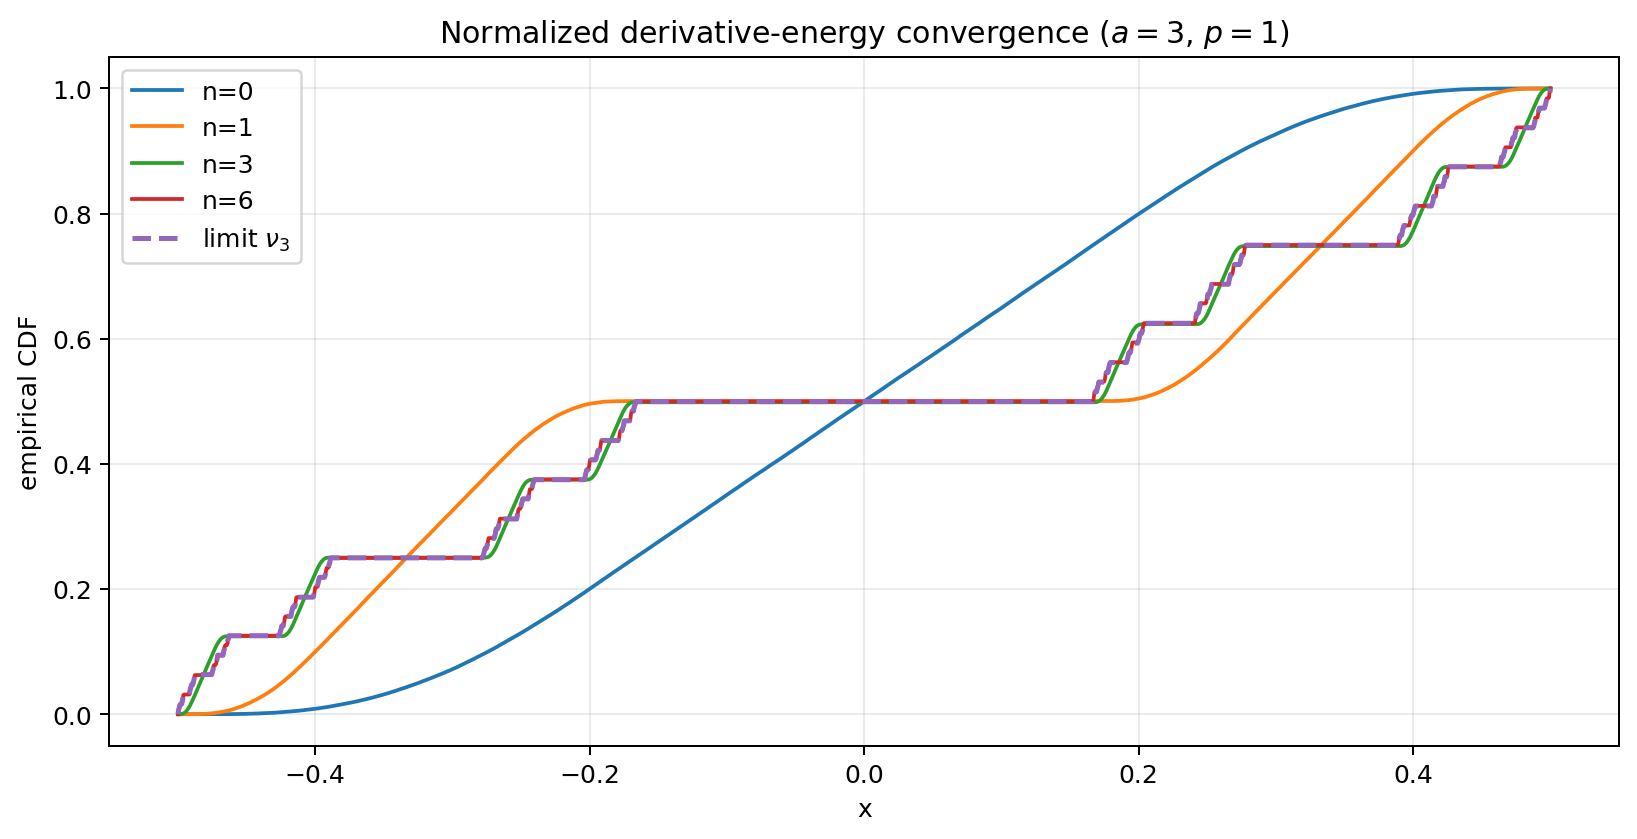
\includegraphics[width=0.92\textwidth]{assets/Atomic_Functions_Beyond_Dyadic_Frontiers/figures/derivative_energy_cantor_limit_a_3.png}
\caption{Distribution functions of the normalized $p=1$ derivative-energy
measures $\mu_{3,n,1}$ for increasing $n$, against the Bernoulli-convolution
limit $\nu_3$ (\cref{p6:thm:energy-factorization}).  The exact coupling
error \eqref{p6:eq:energy-winfty} is at most $3^{-n}$.}
\label{p6:fig:energy-cantor}
\end{figure}

\section{Spectral moments and the Stieltjes--Wigert bridge}
\label{p6:sec:spectral-sw}

The $p=2$ rung of the ladder has a moment-theoretic consequence (revised
fourteenth wave): the Fourier energy of every $h_a$, $a\ge2$, is an explicit
representing measure for a scaled Stieltjes--Wigert moment problem.

\subsection{The spectral probability law and its moments}

In the source's angular variable, let $T_a$ have the symmetric probability
density $|\widehat h_a(t/2\pi)|^2/I_a$ with
$I_a=\int_\R|\widehat h_a(t/2\pi)|^2\dd t=2\pi\|h_a\|_2^2$, and put
$Z_a=T_a^2$.

\begin{theorem}[General-base spectral moments]\label{p6:thm:spectral-moments}
For every $a\ge2$ and $n\ge0$,
\begin{equation}\label{p6:eq:spectral-moments}
 \boxed{\ \E\,Z_a^{\,n}
 =\frac{\|h_a^{(n)}\|_2^2}{\|h_a\|_2^2}
 =\frac{a^{\,n(n+2)}}{2^{\,n}}.\ }
\end{equation}
\end{theorem}

\begin{proof}
Parseval converts frequency moments into derivative energies,
$\int t^{2n}|\widehat h_a(t/2\pi)|^2\dd t=2\pi\|h_a^{(n)}\|_2^2$, and the
$p=2$ case of \cref{p6:thm:equimeasurability} gives
$\|h_a^{(n)}\|_2^2/\|h_a\|_2^2
=C_{a,n}^2(2/a)^n=a^{n(n+2)}/2^n$.
\end{proof}

\begin{corollary}[A continuum of non-lognormal moment twins]
\label{p6:cor:lognormal-twins}
Let $Z_a^{\mathrm{ln}}$ be lognormal with
$\log Z_a^{\mathrm{ln}}\sim N(2\log a-\log2,\ 2\log a)$.  Then
$\E(Z_a^{\mathrm{ln}})^n=a^{n(n+2)}/2^n=\E Z_a^n$ for all $n$, but the two
laws are distinct: the spectral density behaves like $I_a^{-1}z^{-1/2}$ as
$z\downarrow0$, whereas the lognormal density vanishes faster than every
power.  Hence this Stieltjes moment sequence is indeterminate
(Heyde's classical lognormal indeterminacy~\cite{p6:heyde}), and the sinc
product supplies, for every base $a\ge2$, a concrete second representing
density.
\end{corollary}

\subsection{The scaled Stieltjes--Wigert package}

With $q=a^{-2}$ and $c=a/2$, the moments read
$m_n=c^nq^{-n(n+1)/2}$: the Stieltjes--Wigert sequence after the dilation
$z\mapsto cz$.  The refinement equation gives the two moment twins distinct
exact $q$-Pearson scale equations,
\begin{equation}\label{p6:eq:q-pearson}
 w_{\mathrm{sp}}(a^2z)=\frac1a\,
 \operatorname{sinc}^2(\sqrt z\,)\,w_{\mathrm{sp}}(z),
 \qquad
 w_{\mathrm{ln}}(a^2z)=\frac1{2az}\,w_{\mathrm{ln}}(z),
\end{equation}
(the spectral one from $\widehat h_a$'s one-step refinement, written in the
angular variable), and the shared moment functional has closed Hankel
determinants and monic orthogonal polynomials:
\begin{gather}
 \Delta_N=\det[m_{i+j}]_{i,j=0}^{N}
 =c^{\,N(N+1)}\,q^{-N(N+1)(4N+5)/6}
 \prod_{k=1}^{N}(q;q)_k,
 \label{p6:eq:sw-hankel}\\
 P_{a,n}(z)=\sum_{k=0}^{n}(-1)^{n-k}c^{\,n-k}q^{\,k^2-n^2}
 \qbinom nk q\,z^k,
 \qquad
 \int_0^\infty P_{a,n}^2\dd\rho
 =c^{2n}q^{-n(2n+1)}(q;q)_n,
 \label{p6:eq:sw-op}
\end{gather}
for either representing measure $\rho$ --- the dilated monic
Stieltjes--Wigert system~\cite{p6:ismail}.  (Hankel: factor
$c^{i+j}q^{-i(i+1)/2-j(j+1)/2-ij}$ from rows and columns and evaluate the
Vandermonde determinant in $1,q^{-1},\ldots,q^{-N}$; the squared norm is
$\Delta_n/\Delta_{n-1}$.)  The repository's $q$-moment algebra thus acquires,
from the derivative thinning law alone, a one-parameter family of concrete
sinc-product representatives of the scaled Stieltjes--Wigert moments.  The
open Nevanlinna--Pick question for this family is recorded in
\cref{p6:sec:future-directions}.

\begin{figure}[H]
\centering

\includegraphics[width=0.9\textwidth]{assets/Atomic_Functions_Beyond_Dyadic_Report-2/figures/spectral_lognormal_general_base.png}
\caption{The spectral density of $Z_a$ against its lognormal moment twin for
representative bases.  The two densities share every moment
\eqref{p6:eq:spectral-moments} yet differ on an interval
(\cref{p6:cor:lognormal-twins}).}
\label{p6:fig:spectral-lognormal}
\end{figure}

\section{The derivative tower as a \texorpdfstring{$q$}{q}-Gaussian Riesz sequence}
\label{p6:sec:q-gaussian-tower}

The $L^2$ ladder also fixes every \emph{mutual} inner product of the
derivatives (revised and expanded editions of both reconstructions), and
the resulting Hilbert-space geometry is exactly solvable --- down to a
closed Gram--Schmidt process, an explicit unitary circle model, and a
compactly supported Stieltjes--Wigert ladder in physical space.

\begin{theorem}[Exact derivative Gram kernel]\label{p6:thm:derivative-gram}
Let $a>2$ and $\psi_n=h_a^{(n)}/\|h_a^{(n)}\|_2$.  Then
$\langle\psi_n,\psi_m\rangle=0$ for $n-m$ odd and
\begin{equation}\label{p6:eq:derivative-gram}
 \langle\psi_n,\psi_m\rangle
 =(-1)^{(n-m)/2}\,a^{-(n-m)^2/4}
 \qquad(n-m\ \text{even}).
\end{equation}
Consequently, for each parity $\epsilon\in\{0,1\}$ the sign-corrected tower
$\eta_j=(-1)^j\psi_{2j+\epsilon}$ has the stationary $q$-Gaussian kernel
\begin{equation}\label{p6:eq:q-gaussian-kernel}
 \boxed{\ \langle\eta_j,\eta_k\rangle=q^{(j-k)^2},
 \qquad q=a^{-1},\ }
\end{equation}
and the even and odd towers are mutually orthogonal.
\end{theorem}

\begin{proof}
Parity of $h_a^{(n)}$ is $(-1)^n$, killing odd differences.  For $n=m+2r$,
$r$ integrations by parts give
$\langle h_a^{(m+2r)},h_a^{(m)}\rangle=(-1)^r\|h_a^{(m+r)}\|_2^2$.
Normalizing by $\|h_a^{(s)}\|_2^2=a^{s(s+2)}2^{-s}\|h_a\|_2^2$
(\cref{p6:thm:spectral-moments}) at $s=(n+m)/2$ cancels every power of $2$,
and the $a$-exponent is
$s(s+2)-\tfrac12[n(n+2)+m(m+2)]=-(n-m)^2/4$.  The sign correction
$(-1)^{j+k}$ absorbs $(-1)^{(n-m)/2}=(-1)^{j-k}$.
\end{proof}

\begin{theorem}[Gram determinants, pivots, and sharp Riesz bounds]
\label{p6:thm:gram-package}
For $0<q<1$ and $G_N(q)=[q^{(i-j)^2}]_{i,j=0}^N$,
\begin{equation}\label{p6:eq:gram-determinant}
 \boxed{\ \det G_N(q)=\prod_{d=1}^{N}(1-q^{2d})^{N+1-d}
 =\prod_{r=1}^{N}(q^2;q^2)_r,\ }
\end{equation}
so the squared Gram--Schmidt pivot of $\eta_N$ against its predecessors is
$\det G_N/\det G_{N-1}=(q^2;q^2)_N$.  Moreover, for every finitely supported
$(c_j)$,
\begin{equation}\label{p6:eq:riesz-bounds}
 \vartheta_4(0,q)\sum_j|c_j|^2
 \le\Bigl\|\sum_jc_j\eta_j\Bigr\|_2^2
 \le\vartheta_3(0,q)\sum_j|c_j|^2,
\end{equation}
with both Jacobi-theta constants optimal: each parity tower is a Riesz
sequence in $L^2(\R)$.  Since the parity blocks are orthogonal and carry the
same kernel, the \emph{complete} normalized sequence $(\psi_n)_{n\ge0}$ is a
Riesz sequence with the same optimal constants, and the full Gram
determinants factor by parity,
$D_{2N}=(\det G_{N-1})^2$ and $D_{2N+1}=\det G_N\det G_{N-1}$.
\end{theorem}

\begin{proof}
Factoring $q^{i^2}$ from row $i$ and $q^{j^2}$ from column $j$ leaves the
Vandermonde matrix $((q^{-2i})^j)$; the extracted powers cancel against the
$q^{-2\sum j^2}$ from the Vandermonde product, and each difference $d=j-i$
occurs $N+1-d$ times.  For the bounds, the quadratic form has Toeplitz symbol
$\Theta_q(\theta)=\sum_kq^{k^2}\e^{\ii k\theta}=\vartheta_3(\theta/2,q)$,
whose Jacobi triple product
$\prod_r(1-q^{2r})(1+2q^{2r-1}\cos\theta+q^{4r-2})$ is factorwise increasing
in $\cos\theta$: the extremes are $\vartheta_4(0,q)$ at $\theta=\pi$ and
$\vartheta_3(0,q)$ at $0$, attained asymptotically by concentrated Fej\'er
sequences.
\end{proof}

The determinants converge to a classical constant (expanded fifteenth wave):
rearranging \eqref{p6:eq:gram-determinant} as
$\det G_N=(q^2;q^2)_N^{\,N+1}\prod_{d=1}^N(1-q^{2d})^{-d}$ gives exactly
\begin{equation}\label{p6:eq:macmahon}
 \det G_N(q)
 =(q^2;q^2)_\infty^{\,N+1}\,
 \mathfrak M(q^2)\,\bigl(1+\bigO(Nq^{2N})\bigr),
 \qquad
 \mathfrak M(x)=\prod_{d\ge1}(1-x^d)^{-d},
\end{equation}
with $\mathfrak M$ MacMahon's plane-partition generating function
\cite{p6:andrews}: the per-vector entropy of the tower is
$\log(q^2;q^2)_\infty$ and the excess constant counts plane partitions at
$x=a^{-2}$.  The sharp Riesz constants themselves close up under the Jacobi
triple product,
\begin{equation}\label{p6:eq:riesz-triple}
 A_a=\vartheta_4(0,q)=(q^2;q^2)_\infty\,(q;q^2)_\infty^2,
 \qquad
 B_a=\vartheta_3(0,q)=(q^2;q^2)_\infty\,(-q;q^2)_\infty^2,
\end{equation}
with values
\begin{center}
\begin{tabular}{cccc}
\toprule
$a$ & $A_a$ & $B_a$ & $B_a/A_a$\\
\midrule
$2$  & $0.1211242080$ & $2.1289368272$ & $17.5765$\\
$3$  & $0.3579231273$ & $1.6914596817$ & $\phantom{1}4.7258$\\
$4$  & $0.5078048711$ & $1.5078201299$ & $\phantom{1}2.9693$\\
$10$ & $0.8001999980$ & $1.2002000020$ & $\phantom{1}1.4999$\\
\bottomrule
\end{tabular}
\end{center}
The theorem ties the Rvachev derivative tower to Gaussian
Toeplitz kernels, Jacobi theta functions, and finite $q$-Pochhammer products
at once, and shows that --- in stark contrast to the explosive unnormalized
norms --- the normalized towers stay uniformly well conditioned no matter how
many derivatives are taken: even at the critical base $a=2$ the condition
number of the full infinite tower is $B_2/A_2\approx17.58$, and it decays to
$1$ like $4q$ as $a\to\infty$.

\begin{figure}[H]
\centering

\includegraphics[width=0.92\textwidth]{assets/Atomic_Functions_Rvachev_Report_Package/figures/derivative_gram_spectrum.png}
\caption{Eigenvalues of the finite $q$-Gaussian derivative Gram matrices at
$a=3$ against the sharp infinite Riesz bounds $\vartheta_4(0,\tfrac13)$ and
$\vartheta_3(0,\tfrac13)$ (\cref{p6:thm:gram-package}).}
\label{p6:fig:gram-spectrum}
\end{figure}

\subsection{Closed orthogonalization: Gaussian binomials and Rogers--Szeg\H{o} innovations}

The Gram--Schmidt process for the stationary kernel
\eqref{p6:eq:q-gaussian-kernel} is itself exactly solvable (expanded
fifteenth-wave editions): the orthogonal directions, the Cholesky
factorization, and the inverse Gram matrix are all single
Gaussian-binomial sums, the residuals are nodal polynomials at geometric
nodes, and the limiting innovation filter is an explicit theta spectral
factor.

\begin{theorem}[Closed $q$-Gram--Schmidt]\label{p6:thm:q-gram-schmidt}
Fix a parity $\epsilon$ and abbreviate $e_j=\psi_{2j+\epsilon}$, the raw
normalized derivatives, whose Gram matrix is the \emph{signed} kernel
$\widetilde G_N=[(-1)^{i-j}q^{(i-j)^2}]_{i,j=0}^{N}$ of
\cref{p6:thm:derivative-gram}.  The vectors
\begin{equation}\label{p6:eq:q-gram-schmidt}
 \boxed{\ \psi_n^{\ast}
 =\sum_{j=0}^{n}q^{\,n-j}\qbinom{n}{j}{q^2}\,e_j\ }
\end{equation}
satisfy $\langle\psi_n^{\ast},e_k\rangle=0$ for $0\le k<n$ and
$\langle\psi_n^{\ast},e_n\rangle=\|\psi_n^{\ast}\|_2^2=(q^2;q^2)_n$: up to
normalization, $\psi_n^{\ast}$ is the $n$-th Gram--Schmidt vector of the
tower.  Equivalently, the unit lower-triangular matrix
$C=\bigl[\,q^{\,n-j}\qbinom{n}{j}{q^2}\,\bigr]_{n\ge j\ge0}$ factors the
raw kernel and its inverse explicitly:
\[
 C\,\widetilde G_N\,C^{\mathsf T}
 =\operatorname{diag}\bigl((q^2;q^2)_0,\ldots,(q^2;q^2)_N\bigr),
 \qquad
 (\widetilde G_N^{-1})_{jk}
 =\sum_{n=\max(j,k)}^{N}
 \frac{q^{\,2n-j-k}}{(q^2;q^2)_n}
 \qbinom{n}{j}{q^2}\qbinom{n}{k}{q^2},
\]
re-deriving the determinant \eqref{p6:eq:gram-determinant} and its pivots.
In the sign-corrected basis $\eta_j=(-1)^je_j$ of
\eqref{p6:eq:q-gaussian-kernel} the coefficients simply alternate:
$(-1)^n\psi_n^{\ast}=\sum_j(-q)^{\,n-j}\qbinom{n}{j}{q^2}\,\eta_j$ is the
$n$-th Gram--Schmidt vector there, and the positive kernel
$G_N=[q^{(i-j)^2}]$ of \cref{p6:thm:gram-package} has
$(G_N^{-1})_{jk}=(-1)^{j-k}(\widetilde G_N^{-1})_{jk}$; determinants,
pivots, and distances are unchanged, since the two kernels are conjugate by
$\operatorname{diag}\bigl((-1)^i\bigr)$.
\end{theorem}

\begin{proof}
The $q$-binomial theorem at base $q^2$ reads
$\sum_{j=0}^n\qbinom{n}{j}{q^2}q^{\,j(j-1)}x^j=\prod_{r=0}^{n-1}(1+q^{2r}x)$.
Since $q^{\,n-j}(-1)^{j-k}q^{(j-k)^2}
=(-1)^kq^{\,n+k^2}\cdot q^{\,j(j-1)}(-q^{-2k})^j$,
\[
 \langle\psi_n^{\ast},e_k\rangle
 =\sum_{j=0}^{n}q^{\,n-j}\qbinom{n}{j}{q^2}\,(-1)^{j-k}q^{(j-k)^2}
 =(-1)^kq^{\,n+k^2}\prod_{r=0}^{n-1}\bigl(1-q^{2(r-k)}\bigr).
\]
For $0\le k<n$ the factor $r=k$ vanishes.  At $k=n$ the product telescopes
to $(-1)^nq^{-n(n+1)}(q^2;q^2)_n$ and the prefactor $(-1)^nq^{\,n+n^2}$
cancels sign and power exactly.  Expanding $\|\psi_n^{\ast}\|_2^2$ against
the defining sum \eqref{p6:eq:q-gram-schmidt} then keeps only the $j=n$
term.  The two matrix identities are the same computation read as
$C\widetilde G_NC^{\mathsf T}=D$ and
$\widetilde G_N^{-1}=C^{\mathsf T}D^{-1}C$; conjugating by
$\operatorname{diag}((-1)^i)$ transports both to the sign-corrected
basis.
\end{proof}

The expanded fifteenth-wave editions add two closures: the residuals are
nodal polynomials at geometric nodes, and the triangular transform has an
equally explicit inverse.

\begin{theorem}[Nodal form and the exact inverse transform]
\label{p6:thm:gs-nodal-inverse}
Write $Q=q^2$ and
$r_n=(-1)^n\psi_n^{\ast}=\sum_{k}(-q)^{\,n-k}\qbinom{n}{k}{Q}\,\eta_k$
for the monic Gram--Schmidt residuals of the sign-corrected tower.
\begin{enumerate}
\item The generating polynomial
$P_n(z)=\sum_k(-1)^{n-k}q^{\,n-k}\qbinom{n}{k}{Q}q^{\,k^2}z^k$ factors as
the nodal product
\begin{equation}\label{p6:eq:gs-nodal}
 P_n(z)=q^{\,n^2}\prod_{j=0}^{n-1}\bigl(z-q^{-2j}\bigr),
 \qquad
 \langle r_n,\eta_j\rangle=q^{\,j^2}P_n\bigl(q^{-2j}\bigr):
\end{equation}
orthogonality is interpolation at the geometric nodes
$1,Q^{-1},\ldots,Q^{-(n-1)}$, and the pivot is the evaluation at the next
node, $\|r_n\|_2^2=q^{\,n^2}P_n(q^{-2n})=(Q;Q)_n$.
\item The transform inverts in closed form:
\begin{equation}\label{p6:eq:gs-inverse}
 \boxed{\ \eta_n=\sum_{k=0}^{n}q^{(n-k)^2}\qbinom{n}{k}{Q}\,r_k,\ }
\end{equation}
that is, $C'_{nk}=(-q)^{\,n-k}\qbinom{n}{k}{Q}$ and
$B_{nk}=q^{(n-k)^2}\qbinom{n}{k}{Q}$ satisfy $C'_NB_N=B_NC'_N=I$, and the
positive kernel factors as
$G_N=B_ND_NB_N^{\mathsf T}$ with
$D_N=\operatorname{diag}\bigl((Q;Q)_0,\ldots,(Q;Q)_N\bigr)$: the Cholesky
factor of the strictly totally positive kernel is itself entrywise
positive.
\end{enumerate}
\end{theorem}

\begin{proof}
Since $q^{\,n-k}q^{\,k^2}=q^{\,n}Q^{\binom k2}$, Gauss's identity
$\sum_k(-1)^kQ^{\binom k2}\qbinom{n}{k}{Q}z^k=(z;Q)_n$ gives
$P_n(z)=(-1)^nq^{\,n}(z;Q)_n=q^{\,n^2}\prod_j(z-q^{-2j})$, and
$(k-j)^2=k^2-2kj+j^2$ turns $\langle r_n,\eta_j\rangle$ into
$q^{\,j^2}P_n(q^{-2j})$.  The nodes $j<n$ annihilate; at $j=n$,
extracting $q^{-2n}$ from each factor of $P_n(q^{-2n})$ leaves
$(Q;Q)_n\,q^{-2n^2}$, and the prefactors $q^{\,n^2}\cdot q^{\,n^2}$
cancel exactly.  For the inverse, put $d=n-m$ and $j=k-m$; the trinomial identity
$\qbinom{n}{k}{Q}\qbinom{k}{m}{Q}
=\qbinom{n}{m}{Q}\qbinom{d}{j}{Q}$ gives
\[
 \sum_{k=m}^{n}B_{nk}C'_{km}
 =\qbinom{n}{m}{Q}\sum_{j=0}^{d}(-1)^jq^{(d-j)^2+j}\qbinom{d}{j}{Q}
 =\qbinom{n}{m}{Q}(-1)^dq^{\,d}
 \sum_{i=0}^{d}(-1)^iQ^{\binom i2}\qbinom{d}{i}{Q},
\]
substituting $i=d-j$ and $q^{\,i^2-i}=Q^{\binom i2}$; the inner sum is
$(1;Q)_d$ by Gauss, which vanishes for $d\ge1$ and is $1$ at $d=0$.  Triangularity makes the one-sided inverse
two-sided, and $C'G_NC'^{\mathsf T}=D_N$ rearranges to
$G_N=B_ND_NB_N^{\mathsf T}$.
\end{proof}

\begin{remark}[Exact formal boundary for the q-Gaussian inverse]
Only the coefficient-inversion component of the preceding two theorems is
currently exact in Lean.  In
\path{QBinomialInversionSpecializations.lean}, at Gaussian base \(Q=q^2\) and
independent scale \(s=-q\), the definitions
\lean{Fabius.qGaussianResidualCoeff} and
\lean{Fabius.qGaussianReconstructionCoeff} have the closed forms
\[
 C'_{n,k}=(-q)^{n-k}{n\brack k}_{q^2},
 \qquad
 B_{n,k}=q^{(n-k)^2}{n\brack k}_{q^2}
\]
by \lean{Fabius.qGaussianResidualCoeff_eq} and
\lean{Fabius.qGaussianReconstructionCoeff_eq}.  The two declarations
\lean{Fabius.qGaussianReconstructionCoeff_residualCoeff_delta} and
\lean{Fabius.qGaussianResidualCoeff_reconstructionCoeff_delta} prove both
total finite convolutions, hence \(C'_NB_N=B_NC'_N=I\) for every \(N\).
Together with
\lean{Fabius.scaledGaussianBinomialInverseTransform_transform} and
\lean{Fabius.scaledGaussianBinomialTransform_inverseTransform} from
\path{QBinomialTransform.lean}, this proves the module-valued reconstruction
\eqref{p6:eq:gs-inverse} whenever \(r=C'\eta\).  It needs only a commutative
ring acting on an additive commutative monoid; \(q\) need not be nonzero or
invertible.

This does \emph{not} mark all of \cref{p6:thm:q-gram-schmidt} or
\cref{p6:thm:gs-nodal-inverse} formalized.  No current declaration in this
tranche proves the displayed Hilbert inner products or norms, the Gram or
inverse-Gram formulas, the nodal product and its evaluations, the pivots, or
\(G_N=B_ND_NB_N^{\mathsf T}\).  Those analytic and Gram-factorization
components remain open; only \eqref{p6:eq:gs-inverse} and the two-sided
coefficient matrix inverse are exact here.
\end{remark}

\begin{remark}[Rogers--Szeg\H{o} identification]\label{p6:rem:rogers-szegoe}
Substituting $e_j\mapsto z^j$ turns \eqref{p6:eq:q-gram-schmidt} into
$q^nH_n(z/q;q^2)$, where $H_n(z;q)=\sum_j\qbinom{n}{j}{q}z^j$ is the
Rogers--Szeg\H{o} polynomial: the derivative tower of $h_a$ is
orthogonalized by the classical $q$-Hermite circle polynomials at base
$a^{-2}$ \cite{p6:ismail}.  This is forced by \cref{p6:prop:circle-model}
below, because the Rogers--Szeg\H{o} polynomials are precisely the
orthogonal polynomials of the theta weight on the circle.
\end{remark}

\begin{corollary}[Uniform innovation]\label{p6:cor:innovation-distance}
For every $n\ge1$,
\[
 \operatorname{dist}_{L^2}
 \bigl(e_n,\operatorname{span}(e_0,\ldots,e_{n-1})\bigr)^2
 =(q^2;q^2)_n\ \downarrow\ (q^2;q^2)_\infty>0:
\]
no matter how many derivatives have been recorded, the next one retains an
innovation of norm at least $(q^2;q^2)_\infty^{1/2}$ --- new derivatives
never become asymptotically redundant, in sharp contrast with the explosive
growth of the unnormalized norms.
\end{corollary}

\begin{proof}
The squared distance is the Gram--Schmidt pivot
$\det G_n/\det G_{n-1}=(q^2;q^2)_n$ of \cref{p6:thm:gram-package},
decreasing to the convergent infinite product.
\end{proof}

\begin{proposition}[Circle model: the wrapped heat kernel at time $\log a$]
\label{p6:prop:circle-model}
Fix a parity $\epsilon$ and let
\[
 \Theta_a(\theta)
 =\sum_{k}(-1)^kq^{k^2}\e^{\ii k\theta}
 =\vartheta_4\Bigl(\tfrac\theta2,q\Bigr)
 =\sqrt{\frac{\pi}{\log a}}\,
 \sum_{k}\exp\Bigl(-\frac{(\theta-\pi-2\pi k)^2}{4\log a}\Bigr),
 \qquad q=a^{-1},
\]
a strictly positive analytic weight.  Then $\psi_{2j+\epsilon}\mapsto z^j$
extends to a unitary equivalence between
$\overline{\operatorname{span}}\{\psi_{2j+\epsilon}\}_{j\ge0}\subset L^2(\R)$
and the closure of the polynomials in
$L^2\bigl(\mathbb T,\Theta_a\,\frac{d\theta}{2\pi}\bigr)$: each parity tower
of normalized derivatives is the monomial sequence of a weighted Hardy space
whose weight is the wrapped heat kernel at time $\log a$, centred at the
antipode $\theta=\pi$.  The sign correction $e_j=(-1)^j\psi_{2j+\epsilon}$
rotates the weight to $\vartheta_3(\theta/2,q)$, centred at $\theta=0$.
\end{proposition}

\begin{proof}
The monomial Gram matrix of the weight is its Fourier coefficient sequence
$\widehat\Theta_a(j-k)=(-1)^{j-k}q^{(j-k)^2}$, which by
\cref{p6:thm:derivative-gram} is the Gram matrix of the raw tower; a
stationary positive definite kernel determines its closed span up to
canonical unitary equivalence, and the equivalence matches the two
distinguished total sequences.  The theta identity is the Jacobi triple
product; the Gaussian resummation is Poisson summation applied to
$(-1)^kq^{k^2}=\e^{-k^2\log a+\pi\ii k}$.
\end{proof}

Two readings follow.  First, taking two more derivatives of $h_a$ is, in
this model, plain multiplication by the coordinate $z$ --- the most rigid
shift there is; every spectral statement about high derivatives becomes a
statement about a Toeplitz operator with an explicit theta symbol.  Second,
the base $a$ enters only as the heat time $t=\log a$: the family
$a\mapsto\Theta_a$ solves the heat equation on the circle, flattening to the
uniform weight (an asymptotically orthonormal tower) as $a\to\infty$.  The
separated regime only ever sees times $t>\log2$, safely away from the
short-time Dirac degeneration --- which is why the towers stay uniformly
conditioned for all $a>2$, with the table above quantifying the approach to
orthonormality.

The innovation filters themselves stabilize (second expanded
fifteenth-wave edition): far from the left boundary, Gram--Schmidt becomes
an explicit stationary minimum-phase filter.

\begin{theorem}[Minimum-phase theta whitening]\label{p6:thm:theta-whitening}
Write the monic residuals of \cref{p6:thm:gs-nodal-inverse} in lag form,
$r_n=\sum_{r=0}^{n}a_{n,r}\,\eta_{n-r}$ with
$a_{n,r}=(-1)^rq^{\,r}\qbinom{n}{r}{Q}$, $Q=q^2$.  Then
$(a_{n,r})_{r\ge0}\to(a_r)_{r\ge0}$ in $\ell^1$ as $n\to\infty$, where
\[
 a_r=\frac{(-1)^rq^{\,r}}{(Q;Q)_r},
 \qquad
 A_q(z)=\sum_{r\ge0}a_rz^r=\frac1{(-qz;Q)_\infty}
 \qquad(|z|\le1),
\]
whose denominator zeros $z=-q^{-2m-1}$, $m\ge0$, all lie outside the
closed unit disk.  Against the positive Toeplitz symbol
$\vartheta_3(\theta/2,q)=\sum_kq^{k^2}\e^{\ii k\theta}$ of
\cref{p6:thm:gram-package}, Jacobi's triple product gives the exact
whitening identity
\begin{equation}\label{p6:eq:theta-whitening}
 \boxed{\ \bigl|A_q(\e^{\ii\theta})\bigr|^2\,
 \vartheta_3\Bigl(\tfrac\theta2,q\Bigr)=(Q;Q)_\infty
 \qquad(\theta\in\R),\ }
\end{equation}
and $\|r_n\|_2^2=(Q;Q)_n\downarrow(Q;Q)_\infty$ is the stationary
innovation variance of \cref{p6:cor:innovation-distance}.
\end{theorem}

\begin{proof}
For fixed $r$,
$\qbinom{n}{r}{Q}=(Q^{\,n-r+1};Q)_r/(Q;Q)_r\to1/(Q;Q)_r$, with summable
majorant $|a_{n,r}|\le q^{\,r}/(Q;Q)_\infty$, so dominated convergence
gives the $\ell^1$ limit; Euler's theorem
$\sum_rx^r/(Q;Q)_r=1/(x;Q)_\infty$ evaluates the generating function at
$x=-qz$.  The triple product
$\vartheta_3(\theta/2,q)
=(Q;Q)_\infty\,(-q\e^{\ii\theta};Q)_\infty(-q\e^{-\ii\theta};Q)_\infty$
--- the same factorization used for \cref{p6:thm:gram-package} --- divides
out to \eqref{p6:eq:theta-whitening}.
\end{proof}

In prediction-theory language: the finite Gaussian-binomial rows are exact
finite-past innovation filters, and their limit $A_q$ is the causal
minimum-phase Szeg\H{o} spectral factor of the bi-infinite $q$-Gaussian
covariance.  One proof of the closed orthogonalization thus lives at
geometric interpolation nodes (\cref{p6:thm:gs-nodal-inverse}), the other
on the unit circle.  The rate at which the finite rows approach the
stationary filter is posed in the register
(\cref{p6:conj:finite-section}).

Beyond consecutive sections, \emph{every} minor of the kernel is closed,
and positive: the answer is a Schur polynomial.

\begin{theorem}[Schur minors and strict total positivity]
\label{p6:thm:schur-minors}
Let $0<q<1$ and let $0\le r_0<\cdots<r_N$ and $0\le c_0<\cdots<c_N$ be row
and column indices.  With $x_i=q^{-2r_i}$ and the partition
$\lambda=(c_N-N,\ldots,c_1-1,c_0)$,
\begin{equation}\label{p6:eq:schur-minor}
 \boxed{\ \det\bigl[q^{(r_i-c_j)^2}\bigr]_{i,j=0}^{N}
 =q^{\,\sum_ir_i^2+\sum_jc_j^2}
 \prod_{0\le i<j\le N}\!\bigl(x_j-x_i\bigr)\,
 s_\lambda(x_0,\ldots,x_N)\;>\;0.\ }
\end{equation}
Hence the infinite matrix $[q^{(i-j)^2}]_{i,j\ge0}$ is strictly totally
positive.  In particular a sparse parity subfamily
$\eta_{m_0},\ldots,\eta_{m_N}$ has Gram determinant
\[
 q^{\,2\sum_im_i^2}
 \prod_{i<j}\bigl(q^{-2m_j}-q^{-2m_i}\bigr)\,
 s_{(m_N-N,\ldots,m_0)}\bigl(q^{-2m_0},\ldots,q^{-2m_N}\bigr),
\]
recovering \eqref{p6:eq:gram-determinant} at $m_i=i$, where the partition
is empty and the Schur factor is $1$.
\end{theorem}

\begin{proof}
Extract $q^{\,r_i^2}$ from row $i$ and $q^{\,c_j^2}$ from column $j$; the
remaining matrix is the generalized Vandermonde $[x_i^{\,c_j}]$, and the
bialternant definition of Schur polynomials gives
$\det[x_i^{\,c_j}]=\prod_{i<j}(x_j-x_i)\,s_\lambda(x)$.  Since the $r_i$
increase and $q<1$, $0<x_0<\cdots<x_N$: the Vandermonde factor is
positive, and a Schur polynomial has nonnegative coefficients and is
strictly positive at positive arguments.
\end{proof}

\begin{corollary}[Oscillation and the checkerboard inverse]
\label{p6:cor:stp-consequences}
Every finite section of the positive kernel is an oscillation matrix in
Karlin's sense~\cite{p6:karlin}: its Gram maps are variation diminishing,
its eigenvalues are simple and positive, and its inverse has checkerboard
signs --- exactly the $(-1)^{j-k}$ pattern displayed in closed form by
\cref{p6:thm:q-gram-schmidt}.  The Schur factor quantifies how a sparse
choice of derivative orders changes the Euclidean volume of the
normalized system.
\end{corollary}

\begin{figure}[H]
\centering
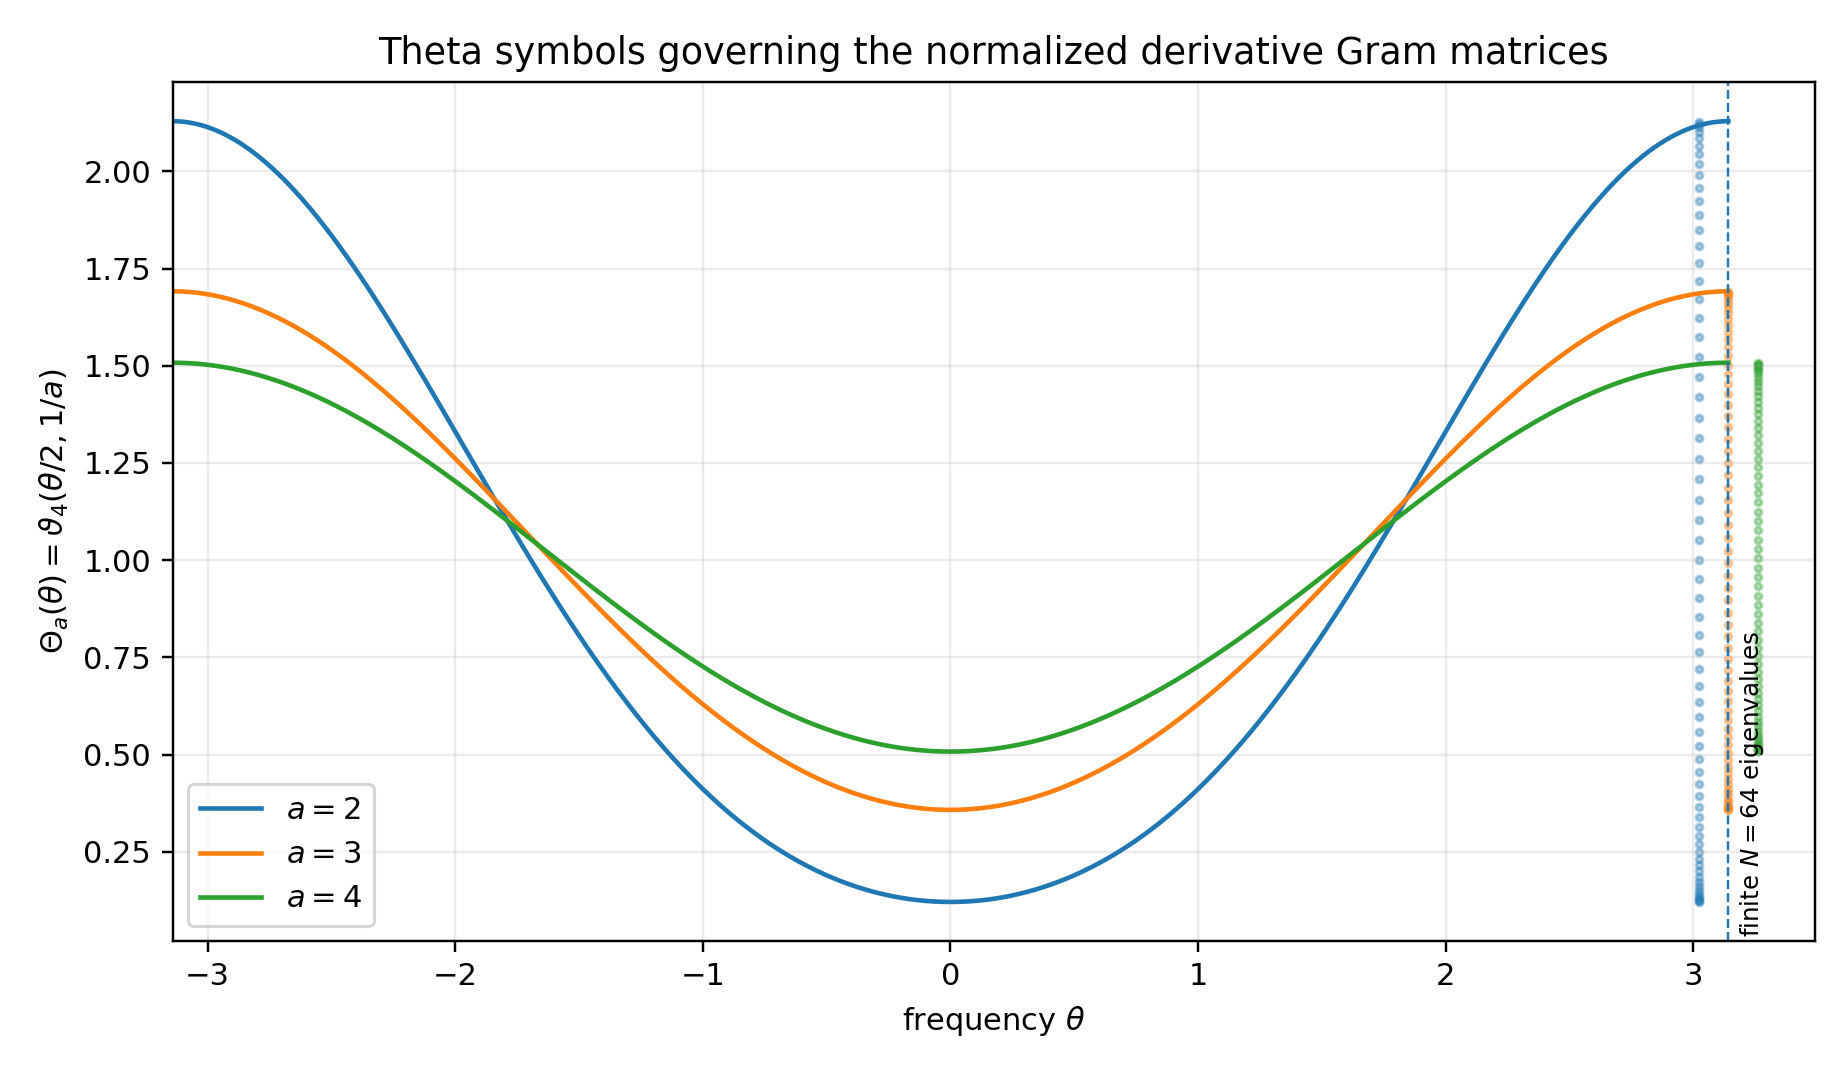
\includegraphics[width=0.92\textwidth]{assets/Atomic_Functions_Rvachev_Expanded_Report/derivative_gram_theta.png}
\caption{The exact Toeplitz symbols $\Theta_a$ for $a=2,3,4$
(\cref{p6:prop:circle-model}).  The vertical point clouds at the right are
the eigenvalues of the corresponding $64\times64$ Gram sections; they lie
inside, and increasingly fill, the optimal theta intervals $[A_a,B_a]$ of
\eqref{p6:eq:riesz-triple}.}
\label{p6:fig:gram-theta}
\end{figure}

\subsection{The physical-space Stieltjes--Wigert ladder and the autocorrelation germ}

The spectral orthogonal polynomials \eqref{p6:eq:sw-op} pull back through
the Fourier transform (expanded fourteenth-wave edition): applied to the
positive operator $\mathcal L=-\dd^2/\dd x^2$, they orthogonalize the
even-derivative span of $h_a$ inside $L^2(\R)$ by the same closed
$q$-binomial formulas, with no Gram--Schmidt recursion.  Here $q=a^{-2}$
and $c=a/2$ as in \cref{p6:sec:spectral-sw}, and
$\dd\rho_{\mathrm{sp}}=w_{\mathrm{sp}}(z)\,\dd z$ denotes the spectral law
of $Z_a$ from \cref{p6:thm:spectral-moments}.

\begin{theorem}[Stieltjes--Wigert differential ladder]\label{p6:thm:sw-ladder}
Let $a\ge2$ and $\Upsilon_{a,n}=P_{a,n}(\mathcal L)h_a$ with $P_{a,n}$ the
monic polynomials \eqref{p6:eq:sw-op}.  Then:
\begin{enumerate}
\item $\widehat{\Upsilon_{a,n}}(t)=P_{a,n}(t^2)\,\widehat h_a(t)$, and each
$\Upsilon_{a,n}$ is $C^\infty$ with support in $[-b_a,b_a]$;
\item the family $\{\Upsilon_{a,n}\}_{n\ge0}$ is orthogonal in $L^2(\R)$,
with
\begin{equation}\label{p6:eq:sw-ladder-norm}
 \|\Upsilon_{a,n}\|_2^2
 =\|h_a\|_2^2\,c^{2n}q^{-n(2n+1)}(q;q)_n;
\end{equation}
\item explicitly, in derivatives,
\begin{equation}\label{p6:eq:sw-ladder-expansion}
 \boxed{\ \Upsilon_{a,n}
 =(-1)^n\sum_{k=0}^{n}c^{\,n-k}q^{\,k^2-n^2}\qbinom nkq\,h_a^{(2k)},\ }
\end{equation}
so $\operatorname{span}\{\Upsilon_{a,0},\ldots,\Upsilon_{a,N}\}
=\operatorname{span}\{h_a,h_a'',\ldots,h_a^{(2N)}\}$ for every $N$;
\item with $\Upsilon_{a,-1}=0$ and $\Upsilon_{a,0}=h_a$, the ladder obeys
the three-term operator recurrence
\begin{equation}\label{p6:eq:sw-ladder-recurrence}
 \Upsilon_{a,n+1}
 =(\mathcal L-\alpha_n)\Upsilon_{a,n}-\beta_n\Upsilon_{a,n-1},
 \qquad
 \begin{aligned}
 \alpha_n&=cq^{-2n-1}\bigl(1+q-q^{\,n+1}\bigr),\\
 \beta_n&=c^2q^{-(4n-1)}\bigl(1-q^n\bigr).
 \end{aligned}
\end{equation}
\end{enumerate}
\end{theorem}

\begin{proof}
$\mathcal L$ acts on the Fourier side as multiplication by $t^2$, so (i) is
polynomial functional calculus, and Parseval turns ladder inner products
into integrals of $P_{a,n}P_{a,m}$ against the spectral law of
\cref{p6:thm:spectral-moments}: orthogonality and
\eqref{p6:eq:sw-ladder-norm} are exactly the statements recorded in
\eqref{p6:eq:sw-op}.  Expanding $P_{a,n}(\mathcal L)$ with
$\mathcal L^k=(-1)^k\partial^{2k}$ collapses the signs
$(-1)^{n-k}(-1)^k$ to the global $(-1)^n$, giving (iii); the change of basis
is triangular with invertible diagonal.  For (iv), the monic three-term
recurrence $zP_{a,n}=P_{a,n+1}+\alpha_nP_{a,n}+\beta_nP_{a,n-1}$ has
$\beta_n=\|P_{a,n}\|^2/\|P_{a,n-1}\|^2$, which \eqref{p6:eq:sw-op}
evaluates to $c^2q^{-(4n-1)}(1-q^n)$, while comparing subleading
coefficients gives
$\alpha_n=p_{n,n-1}-p_{n+1,n}=cq^{-2n-1}(1+q-q^{\,n+1})$, valid also at
$n=0$; substituting $z=\mathcal L$ finishes.
\end{proof}

An indeterminate Stieltjes moment problem in frequency thus produces an
explicit orthogonal system of compactly supported smooth functions in
physical space.  Moreover, the two closed orthogonalizations of the
derivative tower --- this spectral ladder and the $q$-Gaussian
Gram--Schmidt of \cref{p6:thm:q-gram-schmidt} --- are one and the same:

\begin{proposition}[The two ladders coincide]\label{p6:prop:ladder-match}
For every $a\ge2$ and $n\ge0$, the spectral ladder is the even-parity
closed Gram--Schmidt vector, rescaled by the raw derivative norm:
\begin{equation}\label{p6:eq:ladder-match}
 \boxed{\ \Upsilon_{a,n}
 =(-1)^n\,\bigl\|h_a^{(2n)}\bigr\|_2\,\psi_n^{\ast}
 \qquad(\epsilon=0).\ }
\end{equation}
Likewise $(-1)^n\|h_a^{(2n+1)}\|_2\,\psi_n^{\ast}$ at odd parity equals
$\widetilde P_{a,n}(\mathcal L)\,h_a'$, where $\widetilde P_{a,n}$ are the
monic orthogonal polynomials of the once-shifted spectral measure
$z\,\dd\rho_{\mathrm{sp}}(z)$.
\end{proposition}

\begin{proof}
Both sides of \eqref{p6:eq:ladder-match} are orthogonal to
$h_a,h_a'',\ldots,h_a^{(2n-2)}$ and lie in the span through $h_a^{(2n)}$
with the same top coefficient $(-1)^n$ (on the right because
$e_n=h_a^{(2n)}/\|h_a^{(2n)}\|_2$ carries coefficient $1$ in
$\psi_n^{\ast}$); Gram--Schmidt vectors of a flag are unique given the top
coefficient.  Directly: with $q_\ast=a^{-1}$, so that
$\qbinom nk{q_\ast^2}=\qbinom nkq$, the coefficient of $h_a^{(2k)}$ on the
right is $(-1)^n\|h_a^{(2n)}\|_2\,q_\ast^{\,n-k}\qbinom nkq\big/
\|h_a^{(2k)}\|_2$, and the norm ladder \eqref{p6:eq:spectral-moments} gives
$\|h_a^{(2n)}\|_2\,q_\ast^{\,n-k}/\|h_a^{(2k)}\|_2=c^{\,n-k}q^{\,k^2-n^2}$,
matching \eqref{p6:eq:sw-ladder-expansion} term by term; the norms agree
because $\|h_a^{(2n)}\|_2^2\,(q;q)_n
=\|h_a\|_2^2\,c^{2n}q^{-n(2n+1)}(q;q)_n$.  The odd case is the same
argument run on the shifted moments $m_{s+1}$, whose Parseval realization
is $\langle\widetilde P_n(\mathcal L)h_a',\widetilde P_m(\mathcal
L)h_a'\rangle=\|h_a\|_2^2\int\widetilde P_n\widetilde P_m\,z\,
\dd\rho_{\mathrm{sp}}$.
\end{proof}

The unnormalized parity Gram matrices then close in one line each.

\begin{theorem}[Derivative-jet Gram determinants]\label{p6:thm:jet-gram}
For $a\ge2$ and $N\ge0$, put
$E_N^{\mathrm{jet}}=[\langle h_a^{(2i)},h_a^{(2j)}\rangle]_{i,j=0}^{N}$ and
$O_N^{\mathrm{jet}}=[\langle h_a^{(2i+1)},h_a^{(2j+1)}\rangle]_{i,j=0}^{N}$
(mixed parities are orthogonal).  Then
\begin{align}
 \det E_N^{\mathrm{jet}}
 &=\|h_a\|_2^{2(N+1)}\,c^{\,N(N+1)}q^{-N(N+1)(4N+5)/6}
 \prod_{k=1}^{N}(q;q)_k,
 \label{p6:eq:jet-gram-even}\\
 \det O_N^{\mathrm{jet}}
 &=\|h_a\|_2^{2(N+1)}\,c^{\,(N+1)^2}q^{-(N+1)(N+2)(4N+3)/6}
 \prod_{k=1}^{N}(q;q)_k.
 \label{p6:eq:jet-gram-odd}
\end{align}
In particular every finite family of even, and every finite family of odd,
derivatives of $h_a$ is linearly independent in $L^2(\R)$.
\end{theorem}

\begin{proof}
Pull out the norms:
$\det E_N^{\mathrm{jet}}
=\prod_{i=0}^{N}\|h_a^{(2i)}\|_2^2\cdot
\det[\langle\psi_{2i},\psi_{2j}\rangle]$, and the normalized determinant is
$\prod_{r=1}^{N}(q;q)_r$ by \cref{p6:thm:gram-package} (the raw kernel's
alternating signs cancel under conjugation by
$\operatorname{diag}((-1)^i)$).  By \eqref{p6:eq:spectral-moments},
$\prod_{i=0}^{N}\|h_a^{(2i)}\|_2^2
=\|h_a\|_2^{2(N+1)}c^{\,N(N+1)}q^{-N(N+1)(4N+5)/6}$ from
$\sum_{i=0}^{N}i(2i+1)=N(N+1)(4N+5)/6$; the odd case uses
$\sum_{i=0}^{N}(2i+1)(i+1)=(N+1)(N+2)(4N+3)/6$.  The even determinant
equivalently restates the moment Hankel \eqref{p6:eq:sw-hankel}:
$\det E_N^{\mathrm{jet}}=\|h_a\|_2^{2(N+1)}\Delta_N$.
\end{proof}

Finally, the second-order statistics of $X_a$ close at the origin.  Let
$\operatorname{acf}_a=h_a*h_a$, the density of the sum of two independent
copies of $X_a$; since $h_a$ is even, it is also the autocorrelation of
$h_a$, with $\widehat{\operatorname{acf}_a}=\widehat h_a^{\;2}$.

\begin{theorem}[Autocorrelation germ]\label{p6:thm:acf-germ}
For $a\ge2$ and $n\ge0$, all odd derivatives of $\operatorname{acf}_a$
vanish at $0$, and
\begin{equation}\label{p6:eq:acf-germ}
 \boxed{\ \frac{(-1)^n\operatorname{acf}_a^{(2n)}(0)}
 {\operatorname{acf}_a(0)}
 =\frac{\|h_a^{(n)}\|_2^2}{\|h_a\|_2^2}
 =\frac{a^{\,n(n+2)}}{2^{\,n}}.\ }
\end{equation}
The Taylor series of $\operatorname{acf}_a$ at the origin has radius of
convergence zero.
\end{theorem}

\begin{proof}
Fourier inversion gives
$\operatorname{acf}_a^{(2n)}(0)
=(-1)^n(2\pi)^{-1}\int t^{2n}|\widehat h_a(t)|^2\dd t
=(-1)^n\|h_a^{(n)}\|_2^2$ and $\operatorname{acf}_a(0)=\|h_a\|_2^2$; the
moment value is \cref{p6:thm:spectral-moments}.  The $2n$th Taylor
coefficient thus grows like $a^{n^2}$ against $(2n)!=\e^{\bigO(n\log n)}$,
so its $2n$th root diverges.
\end{proof}

\begin{remark}[Plateau versus germ, and incompleteness of the ladder]
For $a>2$ the density $h_a$ is exactly constant on its central plateau,
while its autocorrelation is not analytic at the origin in the strongest
possible sense: the spatial plateau and the frequency-moment explosion
coexist on sharply different analytic levels.  The germ also shows the
ladder is provably \emph{incomplete}: the spectral law
$\rho_{\mathrm{sp}}$ is the spectral measure of $\mathcal L$ in the state
$h_a$, so the cyclic subspace of $h_a$ under $\mathcal L$ is unitarily
$L^2(\rho_{\mathrm{sp}})$ --- but by the Riesz density criterion for
indeterminate moment problems, polynomials are dense in $L^2(\rho)$ only
for $N$-extremal (hence discrete) representing
measures~\cite{p6:ismail}, and $\rho_{\mathrm{sp}}$ is absolutely
continuous.  Hence some vectors $g(\mathcal L)h_a$ of the cyclic subspace
are orthogonal to every even derivative of $h_a$; exhibiting an explicit
bounded one is the subject of \cref{p6:conj:spectral-null-modes}.
\end{remark}

\begin{figure}[H]
\centering
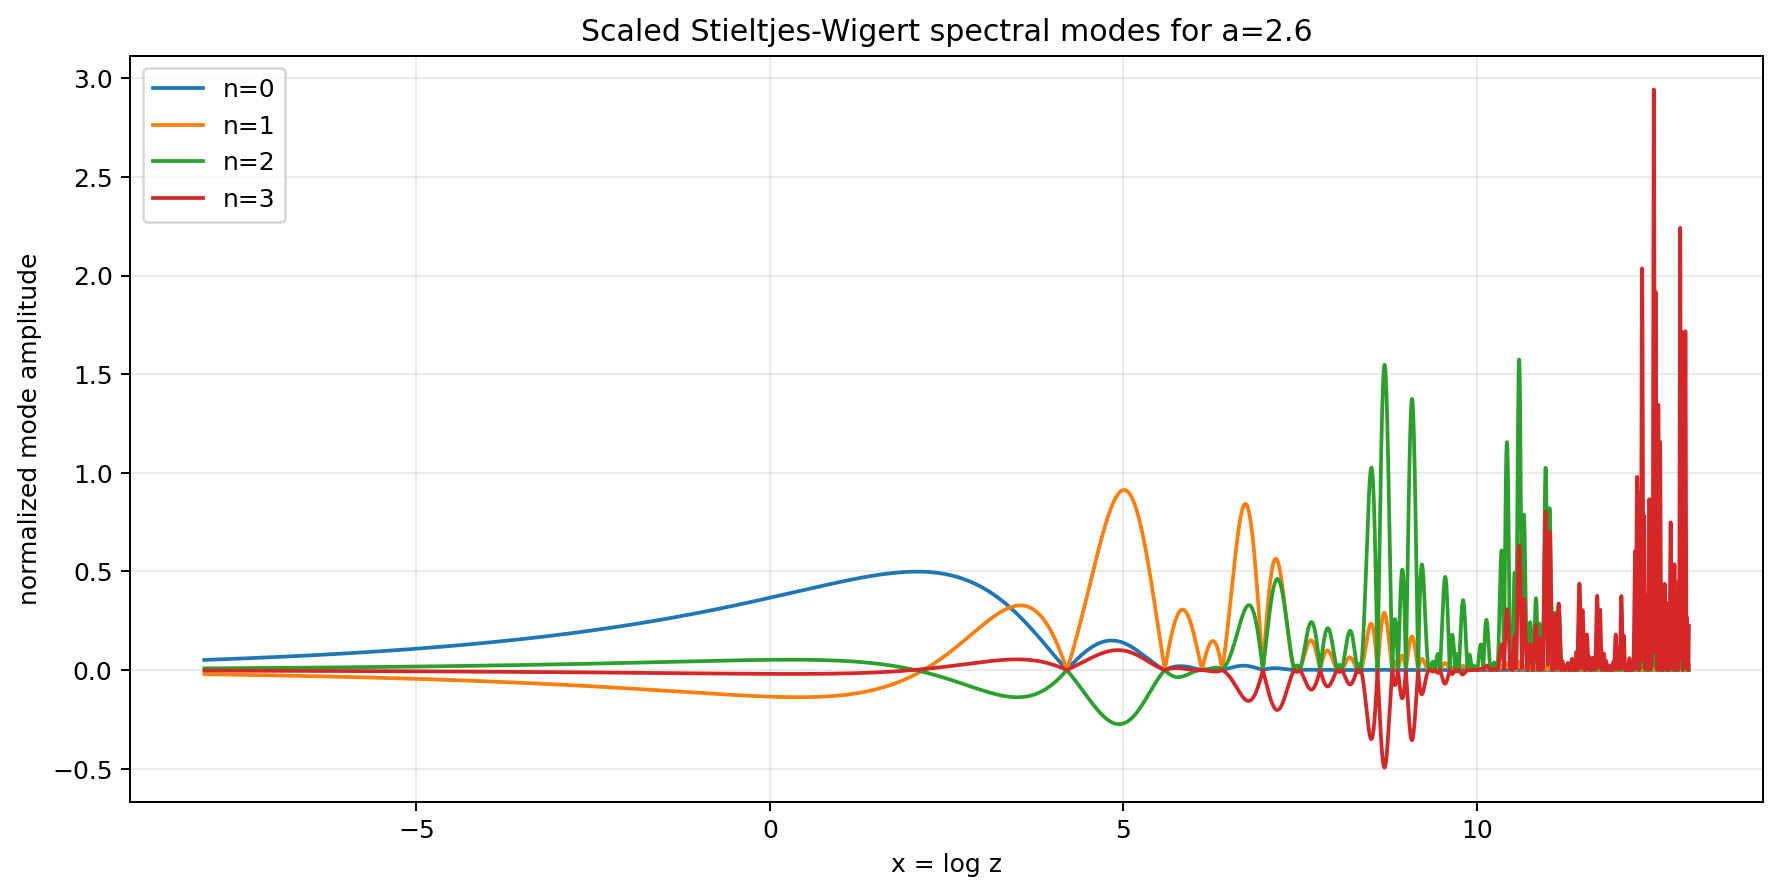
\includegraphics[width=0.92\textwidth]{assets/Atomic_Functions_Beyond_Dyadic_Expanded/figures/orthogonal_derivative_ladder_a_2_6.png}
\caption{The first four normalized spectral modes
$P_{a,n}(t^2)\widehat h_a(t)$ of the differential ladder at $a=2.6$,
displayed against $\log(t^2)$ (\cref{p6:thm:sw-ladder}).  Their numerical
Gram matrix is the identity to the precision recorded in the package's
\texttt{orthogonal\_ladder\_validation\_a\_2\_6.csv}.}
\label{p6:fig:sw-ladder}
\end{figure}

\section{The fractal spline atlas for \texorpdfstring{$a>2$}{a greater than 2}}\label{p6:sec:symbolic-localization}

\subsection{The exceptional self-similar set}

Define the two contractions
\begin{equation}\label{p6:eq:Tpm}
 T_\pm(x)=\frac{x\pm1}{a}
\end{equation}
and their attractor
\begin{equation}\label{p6:eq:Ka}
 K_a=T_-(K_a)\cup T_+(K_a)
 =\left\{
 \sum_{j=1}^{\infty}\varepsilon_ja^{-j}:
 \varepsilon_j\in\{\pm1\}
 \right\}.
\end{equation}
For $a>2$ the two first-level pieces are disjoint.  The open central gap is
\[
 G_\varnothing=(-b_1,b_1),
 \qquad b_1=\frac{a-2}{a(a-1)}.
\]
For a finite word $\omega\in\{-,+\}^r$, let $T_\omega$ be the corresponding
composition and put
\[
 G_\omega=T_\omega(G_\varnothing).
\]

\begin{theorem}[Gap decomposition and dimension]\label{p6:thm:gap-decomposition}
For $a>2$,
\begin{equation}\label{p6:eq:gap-union}
 (-b_a,b_a)\setminus K_a
 =\bigsqcup_{r=0}^{\infty}
 \bigsqcup_{|\omega|=r}G_\omega.
\end{equation}
At depth $r$ there are $2^r$ gaps, each of length $2b_1a^{-r}$, and
\begin{equation}\label{p6:eq:gap-measure-sum}
 \sum_{r=0}^{\infty}2^r(2b_1a^{-r})=2b_a.
\end{equation}
Consequently $K_a$ has Lebesgue measure zero and
\begin{equation}\label{p6:eq:Ka-dimension}
 \dim_{\mathrm H}K_a=\frac{\log2}{\log a}.
\end{equation}
\end{theorem}

\begin{proof}
This is the standard open-set-condition analysis of the two-map iterated
function system.  Removing the first central gap leaves exactly the two scaled
support copies; iterating gives \eqref{p6:eq:gap-union}.  The length calculation is
geometric, and \eqref{p6:eq:gap-measure-sum} follows after substituting
$b_1=b_a(1-2/a)$.  The similarity dimension solves
$2a^{-s}=1$.
\end{proof}

\subsection{Finite spline formula}

Let $h_{a,N}$ be the inverse Fourier transform of the finite product
\begin{equation}\label{p6:eq:Phi-a-N}
 \Phi_{a,N}(\xi)=\prod_{j=1}^{N}
 \sinc(2\pi a^{-j}\xi).
\end{equation}
It is the density of $\sum_{j=1}^{N}a^{-j}U_j$, hence a compact spline of degree
$N-1$.

\begin{theorem}[Explicit finite atomic spline]\label{p6:thm:finite-spline}
For $N\ge1$,
\begin{equation}\label{p6:eq:finite-spline-formula}
 h_{a,N}(x)=
 \frac{a^{N(N+1)/2}}{2^N(N-1)!}
 \sum_{\boldsymbol\varepsilon\in\{\pm1\}^N}
 w(\boldsymbol\varepsilon)
 \left(x+\sum_{j=1}^{N}\varepsilon_ja^{-j}\right)_+^{N-1}.
\end{equation}
Moreover,
\begin{equation}\label{p6:eq:tail-convolution}
 h_a=h_{a,N}*\bigl[a^Nh_a(a^N\,\cdot)\bigr].
\end{equation}
\end{theorem}

\begin{proof}
The density of $a^{-j}U_j$ is
$(a^j/2)\1_{[-a^{-j},a^{-j}]}$.  Repeated integration of the signed endpoint
representation of an interval indicator gives
\eqref{p6:eq:finite-spline-formula}.  Splitting
$X_a=\sum_{j=1}^{N}a^{-j}U_j+a^{-N}X_a'$ gives
\eqref{p6:eq:tail-convolution}.
\end{proof}

The formula makes the $q$-binomial connection concrete: its knots are signed
geometric subset sums, and its coefficients are parity signs.  It also supplies
an exact symbolic implementation independent of FFT inversion, although direct
floating-point evaluation at large $N$ suffers catastrophic cancellation.

\subsection{Local polynomial degree}

\begin{theorem}[Exact degree and derivative amplitude on every gap]
\label{p6:prop:polynomial-gap}
If $|\omega|=r$, then $h_a$ is a polynomial of degree exactly $r$ on
$G_\omega$.  More precisely, throughout that gap,
\begin{equation}\label{p6:eq:gap-leading-derivative}
 \left|h_a^{(r)}(x)\right|
 =\frac{a^{r(r+3)/2+1}}{2^{r+1}},
 \qquad h_a^{(r+1)}(x)=0.
\end{equation}
\end{theorem}

\begin{proof}
On the empty-word gap, $h_a=a/2$, so the assertion holds for $r=0$.
Assume a depth-$r$ gap $G$ has constant nonzero $r$th derivative of magnitude
$C_r$ and vanishing $(r+1)$st derivative.  If $x=T_+(y)=(y+1)/a$ with $y\in G$,
then only the branch $h_a(ax-1)=h_a(y)$ survives in a neighborhood, whereas for
$x=T_-(y)=(y-1)/a$ only $h_a(ax+1)=h_a(y)$ survives.  Differentiating the
one-branch identity $r$ additional times gives
\[
 |h_a^{(r+1)}(x)|=\frac{a^{r+2}}2 C_r,
 \qquad h_a^{(r+2)}(x)=0.
\]
Thus $C_{r+1}=a^{r+2}C_r/2$ with $C_0=a/2$.  Solving this recursion yields
\eqref{p6:eq:gap-leading-derivative}, which is nonzero and proves exact degree.
\end{proof}

This removes the possibility of an exceptional algebraic cancellation: every
word of length $r$ carries a genuinely degree-$r$ piece, with a leading
derivative whose magnitude is the global $r$th-derivative norm.

\begin{corollary}[Signed leading coefficient]\label{p6:cor:signed-leading}
Let $|\omega|=r$ and let $N_+(\omega)$ be the number of $+$ symbols in
$\omega$.  On $G_\omega$ the polynomial piece of $h_a$ has leading coefficient
\begin{equation}\label{p6:eq:signed-leading}
 L_\omega=(-1)^{N_+(\omega)}\,
 \frac{a^{(r+1)(r+2)/2}}{2^{\,r+1}\,r!}.
\end{equation}
\end{corollary}

\begin{proof}
The magnitude is \eqref{p6:eq:gap-leading-derivative} divided by $r!$, since
$a^{r(r+3)/2+1}=a^{(r+1)(r+2)/2}$.  For the sign, follow the one-branch
induction in the proof of \cref{p6:prop:polynomial-gap}: on the image
$T_+(G)$ of a gap $G$ only the branch $-h_a(ax-1)$ of
\eqref{p6:eq:ha-diffeq} survives after differentiation, reversing the sign of
the leading derivative, while on $T_-(G)$ the surviving branch $+h_a(ax+1)$
preserves it.  Starting from the positive plateau value $a/2$ on
$G_\varnothing$, each $+$ letter contributes one sign reversal (fifteenth
wave).
\end{proof}

The first magnitudes at $a=3$ are $\tfrac32$, $\tfrac{27}4$,
$\tfrac{3^6}{16}$, and $\tfrac{3^{10}}{96}$; the fifteenth-wave package
verifies these by polynomial fits on all gaps through generation three.

\subsection{Derivative localization on \texorpdfstring{$K_a$}{K-a}}

For $x\in K_a$, the separated expansion
\begin{equation}\label{p6:eq:digit-expansion}
 x=\sum_{r=1}^{\infty}\varepsilon_ra^{-r}
\end{equation}
is unique.  Define the left shift
\begin{equation}\label{p6:eq:Ta-shift}
 \mathcal T_a^n x
 =\sum_{r=n+1}^{\infty}\varepsilon_ra^{n-r}.
\end{equation}

\begin{theorem}[One-branch symbolic localization]\label{p6:thm:symbolic-localization}
Let $a>2$, $x\in K_a$, and let $(\varepsilon_r)$ be its unique digit sequence.
Then
\begin{equation}\label{p6:eq:symbolic-localization}
 h_a^{(n)}(x)=
 (-1)^n\left(\prod_{r=1}^{n}\varepsilon_r\right)
 \frac{a^{n(n+3)/2}}{2^n}
 h_a(\mathcal T_a^n x).
\end{equation}
\end{theorem}

\begin{proof}
In \eqref{p6:eq:ha-derivative-hierarchy}, choose the sign attached to the power
$a^{n-r}$ to be $-\varepsilon_r$.  Its large prefix cancels
$a^nx$, leaving exactly $\mathcal T_a^nx\in[-b_a,b_a]$.  Any other sign choice
has a first mismatched digit.  Because $a>2$, that leading discrepancy exceeds
the largest possible remaining tail, so the resulting argument lies outside
$[-b_a,b_a]$.  Thus exactly one term survives.  Its weight is
$(-1)^n\prod_{r=1}^{n}\varepsilon_r$, and the common prefactor is the one in
\eqref{p6:eq:exact-derivative-norm}.
\end{proof}

\begin{lemma}[Strict positivity in the open support]\label{p6:lem:positive-interior}
For every $a>1$,
\[
 h_a(x)>0\qquad (|x|<b_a).
\]
\end{lemma}

\begin{proof}
Fix $|x|<b_a$ and choose $N$ so large that $x$ lies in the interior of the
finite-sum support
$[-\sum_{j=1}^N a^{-j},\sum_{j=1}^N a^{-j}]$.  The finite convolution
$h_{a,N}$ is strictly positive in that interior.  Writing
$X_a=X_{a,N}+Z_N$, the tail $Z_N$ assigns positive probability to every
neighborhood of zero (choose finitely many uniform coordinates in small
intervals and bound the remaining geometric tail).  Hence
$h_a(x)=\E[h_{a,N}(x-Z_N)]>0$.
\end{proof}

\begin{corollary}[Terminating Taylor germs]
If the digit sequence of $x\in K_a$ is eventually constant, then
$h_a^{(n)}(x)=0$ for every sufficiently large $n$.  Hence the Taylor series at
$x$ is a polynomial.  Nevertheless $x$ is a gap endpoint, so this polynomial
need not agree with $h_a$ on a neighborhood.
\end{corollary}

\begin{corollary}[A zero-radius criterion]\label{p6:cor:zero-radius-criterion}
Suppose there are a compact set $J\subset K_a\cap(-b_a,b_a)$, a constant
$c_J>0$, and infinitely many $n$ such that
$\mathcal T_a^nx\in J$ and $h_a\ge c_J$ on $J$.  Then the Taylor series of
$h_a$ at $x$ has radius zero.
\end{corollary}

\begin{proof}
Along the stated subsequence,
\[
 |h_a^{(n)}(x)|\ge c_J\frac{a^{n(n+3)/2}}{2^n}.
\]
The $n$th root of $|h_a^{(n)}(x)|/n!$ tends to infinity along that subsequence.
\end{proof}

\begin{theorem}[Complete Taylor-germ classification]\label{p6:thm:taylor-dichotomy}
Let $a>2$.
\begin{enumerate}
\item If $x\notin K_a$, then $x$ lies in a unique polynomial gap and the Taylor
series of $h_a$ agrees locally with the exact polynomial on that gap.
\item If $x\in K_a$ has an eventually constant digit sequence, then its Taylor
series terminates but does not agree with $h_a$ on a full neighborhood.
\item If $x\in K_a$ is not eventually constant, then its Taylor series has
radius zero.
\end{enumerate}
\end{theorem}

\begin{proof}
The first two statements follow from the gap theorem and the terminating-germ
corollary.  For the third, a non-eventually-constant sign sequence has infinitely
many digit changes.  Let $J_a\subset K_a$ be the union of the two compact
second-level cylinders whose first two digits are opposite.  This set is
disjoint from the support endpoints, so by \cref{p6:lem:positive-interior}
$c_a:=\min_{J_a}h_a>0$.  Whenever
$\varepsilon_{n+1}\ne\varepsilon_{n+2}$, the shifted point
$\mathcal T_a^n x$ belongs to $J_a$.  Thus the zero-radius criterion applies
along infinitely many $n$.
\end{proof}

The source states this dichotomy in a longer signed-radix calculation.  The
one-branch formula reduces it to the elementary observation that every
non-eventually-constant binary word contains infinitely many changes.

\begin{remark}[Endpoint jet reduction and the exact engine]
\label{p6:rem:jet-reduction}
At a generation-$n$ cylinder endpoint $x$ the digit sequence is eventually
constant, and the shifted point $\mathcal T_a^{\ell}x$ is again a cylinder
endpoint, of generation $n-\ell$.  \Cref{p6:thm:symbolic-localization} then reads
as an exact jet reduction: for $0\le\ell<n$,
\begin{equation}\label{p6:eq:jet-reduction}
 h_a^{(\ell)}(x)
 =\pm\,\frac{a^{\ell(\ell+3)/2}}{2^{\ell}}\,
 h_a\bigl(\mathcal T_a^{\ell}x\bigr),
\end{equation}
with the sign $(-1)^{\ell}\prod_{r\le\ell}\varepsilon_r$ from the digits
consumed.  The fifteenth-wave package writes \eqref{p6:eq:jet-reduction} in a
fully binary-indexed form with the Thue--Morse sign spelled out, repairing the
damaged source indices (3.51)--(3.58), and combines it with the Taylor
remainder into an explicit chain
\begin{gather*}
 \text{Bernoulli numbers}\to\text{cumulants}\to\text{moments}\\
 \to\text{endpoint values}\to\text{endpoint jets}
 \to\text{every gap polynomial},
\end{gather*}
an exact symbolic engine for $h_a$ over $\Q(a)$ at any algebraic base.  With
\cref{p6:cor:signed-leading} certifying the top coefficient independently, the
engine is self-checking.
\end{remark}

\begin{figure}[H]
\centering
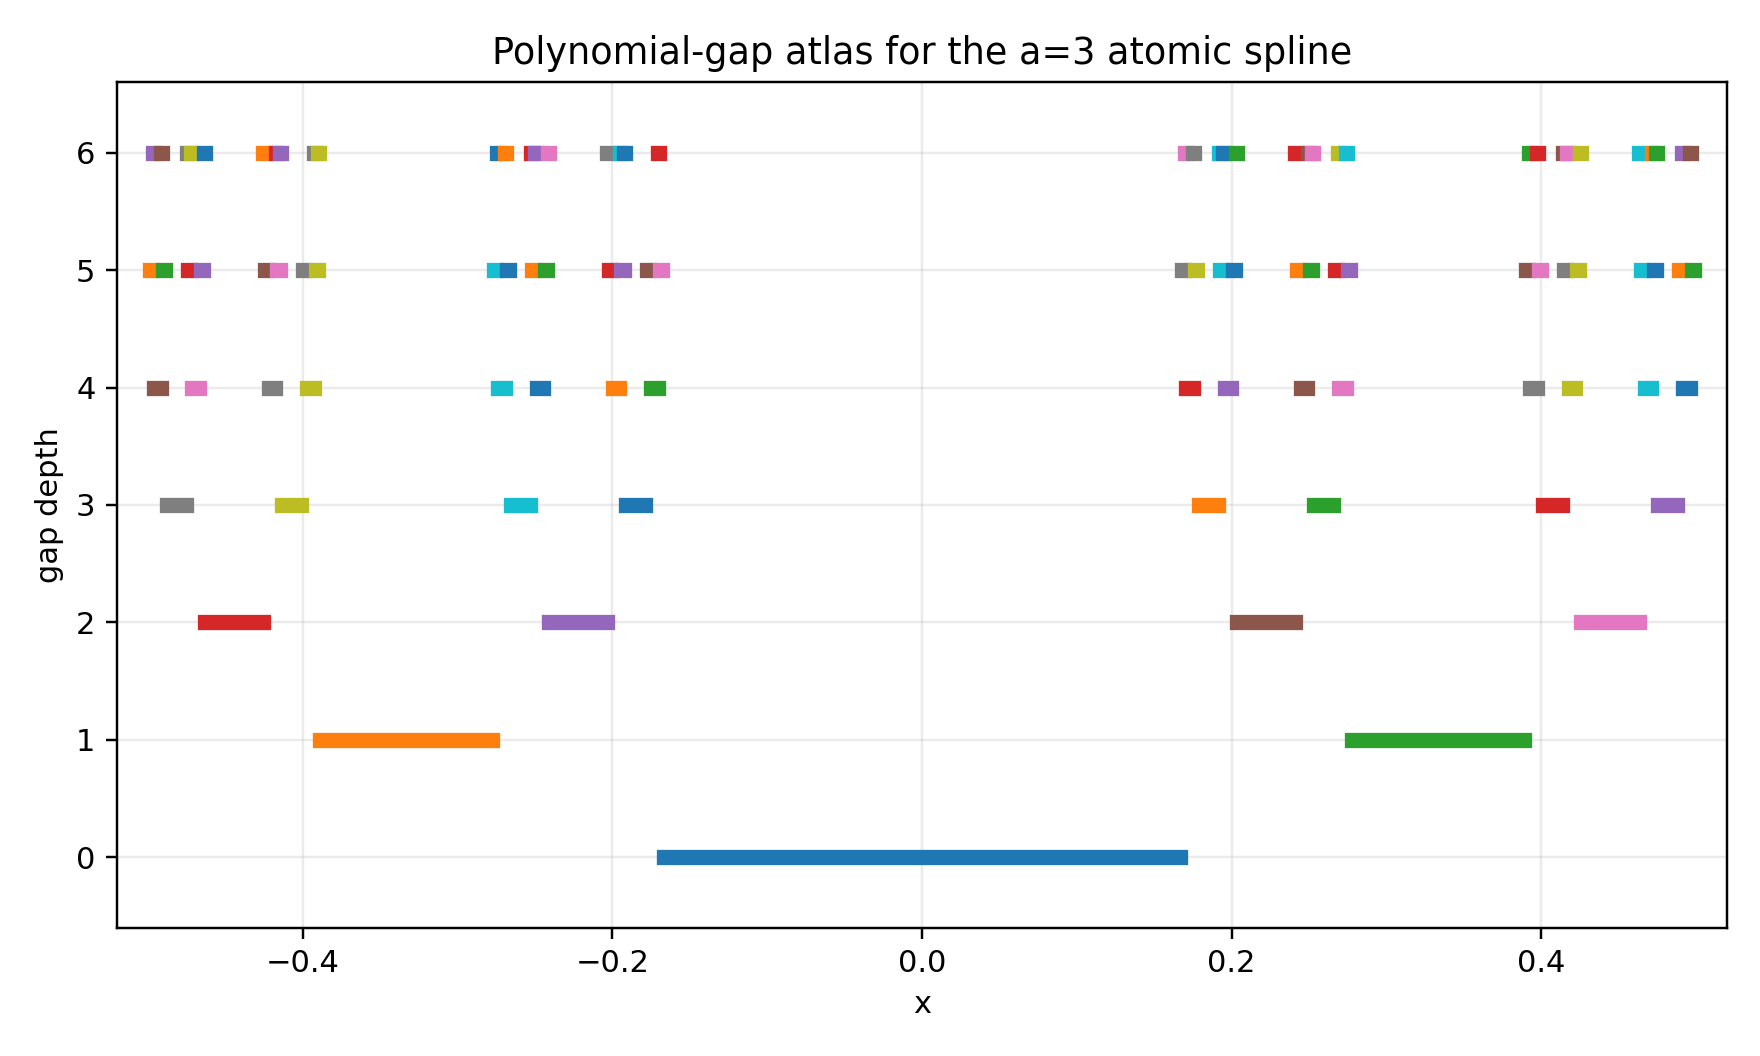
\includegraphics[width=0.94\textwidth]{assets/atomic_sinc_splines_report_package/figures/cantor_gap_atlas_a3.png}
\caption{The first seven levels of the gap decomposition for $a=3$.  The depth
$r$ gaps are the intervals on which the local polynomial degree is exactly $r$.
Their union has full measure in the support $[-1/2,1/2]$.}
\label{p6:fig:cantor-atlas}
\end{figure}

\section{Fractal strings, complex dimensions, and the exact tube formula}
\label{p6:sec:fractal-string}

This section (fourteenth wave) upgrades the qualitative dimension count of
\cref{p6:thm:gap-decomposition} to a complete quantitative geometry of the
exceptional set: every classical statistic of $K_a$---its geometric zeta
function, its complex dimensions, its tube volume, and the distribution of the
local polynomial degree---has a closed form.

\subsection{The gap string and its complex dimensions}

By \cref{p6:thm:gap-decomposition}, the bounded complementary intervals of
$K_a$ form the self-similar fractal string
\begin{equation}\label{p6:eq:gap-string}
 \mathcal L_a:\qquad
 \ell_r=\ell_0a^{-r}
 \ \text{with multiplicity }2^r
 \ (r\ge0),
 \qquad
 \ell_0=2b_1=\frac{2(a-2)}{a(a-1)}.
\end{equation}

\begin{theorem}[Dimension, geometric zeta function, and complex dimensions]
\label{p6:thm:complex-dimensions}
For $a>2$, the Hausdorff and Minkowski dimensions of $K_a$ agree,
\begin{equation}\label{p6:eq:minkowski-dimension}
 \dim_{\mathrm H}K_a=\dim_{\mathrm M}K_a=D_a:=\frac{\log2}{\log a},
\end{equation}
and the geometric zeta function of the string \eqref{p6:eq:gap-string},
\begin{equation}\label{p6:eq:fractal-zeta}
 \zeta_{\mathcal L_a}(s)
 =\sum_{r\ge0}2^r\ell_r^{\,s}
 =\frac{\ell_0^{\,s}}{1-2a^{-s}},
 \qquad\Re s>D_a,
\end{equation}
extends meromorphically to $\C$ with simple poles exactly at the vertical
lattice
\begin{equation}\label{p6:eq:complex-dimensions}
 s_k=D_a+\frac{2\pi\ii k}{\log a},
 \qquad k\in\Z,
 \qquad
 \operatorname*{res}_{s=s_k}\zeta_{\mathcal L_a}(s)
 =\frac{\ell_0^{\,s_k}}{\log a}.
\end{equation}
\end{theorem}

\begin{proof}
The two-map system \eqref{p6:eq:Tpm} satisfies the open-set condition for
$a>2$, so Hutchinson's theorem \cite{p6:hutchinson} gives
$\dim_{\mathrm H}K_a=D_a$ from the similarity equation $2a^{-D}=1$; the tube
formula below shows that $\eps^{D_a-1}V_a(\eps)$ is bounded above and below by
positive constants, which pins the Minkowski dimension at $D_a$ as well.  The
gap sum \eqref{p6:eq:fractal-zeta} is geometric.  Solving $2a^{-s}=1$ gives the
pole lattice, and differentiating the denominator gives
$\dd(1-2a^{-s})/\dd s=2a^{-s}\log a=\log a$ at every $s_k$, hence the residue.
\end{proof}

The vertical arithmetic progression \eqref{p6:eq:complex-dimensions} is the
canonical lattice pattern of a self-similar fractal string in the sense of
Lapidus and van Frankenhuijsen \cite{p6:lapidus-vf}.  What is distinctive here
is that it enters the analysis of a $C^\infty$ function: the singular set of
the smooth spline $h_a$ carries the same complex dimensions as its
complementary gap string.

\subsection{An exact tube formula}

For $\eps>0$, let
\begin{equation}\label{p6:eq:tube-def}
 V_a(\eps)=
 \bigl|\{x\in(-b_a,b_a)\setminus K_a:\operatorname{dist}(x,K_a)<\eps\}\bigr|
\end{equation}
be the inner tube volume.  Each gap of length $\ell$ contributes
$\min(2\eps,\ell)$.

\begin{theorem}[Exact tube formula and Minkowski non-measurability]
\label{p6:thm:tube-formula}
Let $a>2$ and $0<2\eps<\ell_0$, and put
$N(\eps)=\bigl\lfloor\log_a\bigl(\ell_0/(2\eps)\bigr)\bigr\rfloor$.  Then
\begin{equation}\label{p6:eq:exact-tube}
 V_a(\eps)=2\eps\bigl(2^{N(\eps)+1}-1\bigr)
 +\frac{\ell_0\,(2/a)^{N(\eps)+1}}{1-2/a}.
\end{equation}
With $x=\log_a(\ell_0/(2\eps))$ and $\theta=\{x\}$ its fractional part,
\begin{equation}\label{p6:eq:tube-normalized}
 \eps^{D_a-1}V_a(\eps)
 =\mathcal M_a(\theta)-2\eps^{D_a},
\end{equation}
where the one-periodic profile
\begin{equation}\label{p6:eq:minkowski-profile}
 \mathcal M_a(\theta)=\ell_0^{\,D_a}
 \left[
 2^{\,2-D_a-\theta}
 +\frac{2^{\,1-D_a}a^{(D_a-1)(1-\theta)}}{1-2/a}
 \right],
 \qquad0\le\theta<1,
\end{equation}
is continuous under periodic identification and nonconstant.  Hence $K_a$ is
not Minkowski measurable, although its upper and lower Minkowski contents are
finite and positive.  The logarithmic average of the profile is
\begin{equation}\label{p6:eq:average-minkowski}
 \int_0^1\mathcal M_a(\theta)\,\dd\theta
 =\ell_0^{\,D_a}\,2^{\,1-D_a}
 \left(\frac1{\log2}+\frac1{\log(a/2)}\right).
\end{equation}
\end{theorem}

\begin{proof}
The depth-$r$ gaps with $r\le N(\eps)$ are wider than $2\eps$ and contribute
$2\eps$ each; the remaining gaps are covered entirely.  Summing the finite
geometric count and the infinite geometric length tail gives
\eqref{p6:eq:exact-tube}.  Substituting $\eps=(\ell_0/2)a^{-x}$ and using
$a^{D_a}=2$ turns the two terms into
\eqref{p6:eq:tube-normalized}--\eqref{p6:eq:minkowski-profile}; matching the
one-sided limits $\theta\to1^-$ and $\theta=0$ reduces, after dividing by
$2^{1-D_a}$, to the identity $1+\tfrac1{1-2/a}=2+\tfrac{2/a}{1-2/a}$, so the
profile is continuous on the circle.  It is nonconstant because
$2^{-\theta}$ and $a^{(D_a-1)(1-\theta)}$ are nonconstant exponentials with
positive coefficients that are linearly independent from the constants.
Integrating each exponential over one period gives
\eqref{p6:eq:average-minkowski}.  Boundedness of the positive continuous
profile between its minimum and maximum gives finite positive upper and lower
Minkowski contents, and nonconstancy denies Minkowski measurability.
\end{proof}

\begin{figure}[H]
\centering

\includegraphics[width=0.94\textwidth]{assets/Atomic_Functions_Beyond_Dyadic_Report/figures/tube_oscillation_a_3.png}
\caption{The exact normalized tube volume for $a=3$.  The approach to a
nonconstant one-periodic profile in $\log_a(1/\eps)$ verifies the lattice
oscillation of \cref{p6:thm:tube-formula}.}
\label{p6:fig:tube-oscillation}
\end{figure}

\subsection{The local polynomial degree as a random variable}

Choose a point uniformly with respect to normalized Lebesgue measure on
$(-b_a,b_a)$.  Since $K_a$ is null, the point almost surely lies in a unique
gap; let $N_a$ be the exact polynomial degree of $h_a$ on that gap, which by
\cref{p6:prop:polynomial-gap} equals the gap depth.

\begin{theorem}[Geometric degree law and critical exponential limit]
\label{p6:thm:degree-law}
For $a>2$,
\begin{equation}\label{p6:eq:degree-geometric}
 \Prob(N_a=r)=\frac{a-2}{a}\left(\frac2a\right)^{r},
 \qquad r=0,1,2,\ldots,
\end{equation}
so that
\begin{equation}\label{p6:eq:degree-moments}
 \E N_a=\frac2{a-2},
 \qquad
 \operatorname{Var}(N_a)=\frac{2a}{(a-2)^2}.
\end{equation}
With $p_a=(a-2)/a$, as $a\downarrow2$,
\begin{equation}\label{p6:eq:degree-critical-limit}
 p_aN_a\ \xrightarrow{\ d\ }\ \operatorname{Exp}(1),
 \qquad\text{equivalently}\qquad
 \frac{a-2}{2}\,N_a\ \xrightarrow{\ d\ }\ \operatorname{Exp}(1).
\end{equation}
\end{theorem}

\begin{proof}
The total length of the depth-$r$ gaps is $2^r\ell_0a^{-r}$; dividing by
$2b_a=2/(a-1)$ gives \eqref{p6:eq:degree-geometric}, a geometric law on $\N_0$
with success parameter $p_a$, whence \eqref{p6:eq:degree-moments}.  For the
limit,
$\Prob(p_aN_a>x)=(1-p_a)^{\lfloor x/p_a\rfloor+1}\to\e^{-x}$ for every
$x>0$, and $p_a\sim(a-2)/2$.
\end{proof}

This makes the phrase ``polynomial almost everywhere'' quantitative: near the
critical base, a typical polynomial piece has degree of exact order
$(a-2)^{-1}$.  It also identifies the first marginal of the critical
double-scaling program of \cref{p6:sec:future-directions}: the depth variable,
rescaled by $(a-2)/2$, is exponential in the limit, and what remains open is
the joint limit of the word address, the gap geometry, and the polynomial
coefficients.

\begin{figure}[H]
\centering

\includegraphics[width=0.94\textwidth]{assets/Atomic_Functions_Beyond_Dyadic_Report/figures/degree_critical_limit.png}
\caption{Distribution functions of $p_aN_a$ approaching $1-\e^{-x}$ as
$a\downarrow2$ (\cref{p6:thm:degree-law}).}
\label{p6:fig:degree-limit}
\end{figure}

\subsection{Distance to the nonanalytic set and the shifted zeta law}

The revised fourteenth-wave edition refines the degree law into a complete
description of the local geometry seen from a typical point.  Let $Q$ be
uniform on $(-b_a,b_a)$, let $\mathcal G$ be the length of the gap containing
it, and let $\Delta=\operatorname{dist}(Q,K_a)$.

\begin{theorem}[Mellin law of the distance to $K_a$]
\label{p6:thm:distance-mellin}
For $a>2$ there is $V\sim\operatorname{Unif}[0,1]$, independent of $N_a$,
with
\begin{equation}\label{p6:eq:gap-distance-factorization}
 \mathcal G=\ell_0a^{-N_a},
 \qquad
 \Delta\overset d=\frac{\mathcal G}2\,V .
\end{equation}
Consequently, for $\Re s>D_a-1$,
\begin{equation}\label{p6:eq:distance-mellin}
 \E\,\mathcal G^{\,s}
 =\frac{a-2}{a}\,\frac{\ell_0^{\,s}}{1-2a^{-(s+1)}},
 \qquad
 \E\,\Delta^{s}
 =\frac{a-2}{a}\,
 \frac{(\ell_0/2)^{s}}{(s+1)\bigl(1-2a^{-(s+1)}\bigr)},
\end{equation}
with meromorphic continuations whose poles form the shifted lattice
$s=D_a-1+2\pi\ii k/\log a$ (plus the elementary pole $s=-1$ for $\Delta$):
the complex dimensions \eqref{p6:eq:complex-dimensions} reappear, shifted by
$-1$, in the statistics of a Lebesgue-typical point.  Moreover, for
$0<2r<\ell_0$,
\begin{equation}\label{p6:eq:distance-tail-tube}
 \Prob(\Delta>r)=1-\frac{V_a(r)}{2b_a}:
\end{equation}
the exact tube formula \eqref{p6:eq:exact-tube} is also the exact
distribution function of the distance.
\end{theorem}

\begin{proof}
Conditional on $N_a=r$, the point is uniform in one gap of length
$\ell_0a^{-r}$, so its distance to the nearer endpoint is uniform on
$[0,\ell_0a^{-r}/2]$, giving \eqref{p6:eq:gap-distance-factorization} with
$V$ independent of the depth.  Combining with
\eqref{p6:eq:degree-geometric} and summing the geometric series gives
\eqref{p6:eq:distance-mellin}; $\E V^s=1/(s+1)$ supplies the extra factor.
The event $\{\Delta\le r\}$ is the inner $r$-tube of $K_a$ up to the null set
$K_a$ itself.
\end{proof}

\begin{corollary}[Critical logarithmic gap scale]
\label{p6:cor:critical-gap-scale}
As $a\downarrow2$, with $p_a=(a-2)/a$,
\[
 p_a\log_a\frac{\ell_0}{\mathcal G}
 \xrightarrow{\ d\ }\operatorname{Exp}(1),
 \qquad
 p_a\log_a\frac{\ell_0}{2\Delta}
 \xrightarrow{\ d\ }\operatorname{Exp}(1),
\]
since the first variable equals $p_aN_a$ and
$p_a\log_a V\to0$ in probability ($\E(-\log V)=1$); Slutsky's theorem
completes the second.
\end{corollary}

Replacing Lebesgue sampling by $h_a(x)\dd x$ would couple the gap geometry to
the values of the atomic function itself; the resulting weighted distance law
is no longer a geometric series and is left as a further direction.

\begin{figure}[H]
\centering

\includegraphics[width=0.9\textwidth]{assets/Atomic_Functions_Beyond_Dyadic_Report-3/figures/distance_to_singular_set_a_3.png}
\caption{The distance $\Delta$ to the nonanalytic set at $a=3$: empirical
law of a uniform sample against the exact tube-formula distribution
\eqref{p6:eq:distance-tail-tube}.}
\label{p6:fig:distance-set}
\end{figure}

\subsection{Log-Weibull intermittency of the leading jets}

Combining the degree law with the signed leading coefficients quantifies how
violently the highest jets grow (revised fifteenth wave).  Let
$A=|L_\omega|$ be the leading-coefficient magnitude of the gap polynomial at
a uniform point, i.e.\ $A=L_{N_a}$ with
$L_r=a^{(r+1)(r+2)/2}/(2^{r+1}r!)$ by \cref{p6:cor:signed-leading}.

\begin{theorem}[Exact step tail and log-Weibull law]
\label{p6:thm:jet-intermittency}
For $a>2$ the levels $L_r$ are strictly increasing
($L_{r+1}/L_r=a^{r+2}/(2(r+1))>1$), the tail is the exact geometric
staircase
\begin{equation}\label{p6:eq:jet-tail}
 \Prob(A\ge L_r)=\Prob(N_a\ge r)=(2/a)^r,
\end{equation}
and
\begin{equation}\label{p6:eq:jet-log-weibull}
 \lim_{x\to\infty}
 \frac{\log\Prob(A>x)}{\sqrt{\log x}}
 =-\log\!\Bigl(\frac a2\Bigr)\sqrt{\frac2{\log a}}.
\end{equation}
Every positive moment of $A$ diverges, while
$\E[\log(1+A)]^p<\infty$ for all $p>0$; conditional on $N_a=r\ge1$, the sign
of the leading coefficient is a fair Rademacher variable.
\end{theorem}

\begin{proof}
Stirling gives $\log L_r=\tfrac{\log a}2r^2-r\log r+\bigO(r)$, so the
crossing index of level $x$ is $r(x)\sim\sqrt{2\log x/\log a}$; the tail is
constant between consecutive levels and equals $(2/a)^{r(x)}$ up to one
index, giving \eqref{p6:eq:jet-log-weibull}.  For $s>0$ the summands of
$\E A^s$ have logarithms $\tfrac{s\log a}2r^2+\bigO(r\log r)\to\infty$;
$\log(1+L_r)=\bigO(r^2)$ against a geometric law has all polynomial moments.
Exactly half of the $2^r$ depth-$r$ words have even $N_+(\omega)$ for
$r\ge1$.
\end{proof}

A random point almost surely lies on a single finite polynomial piece, yet
increasingly rare pieces carry superexponentially large top coefficients:
spatial sparsity is exponential while amplitude growth is
quadratic-exponential.  This \emph{jet intermittency} warns against judging
numerical conditioning from the almost-everywhere polynomial description
alone, and complements the uniformly well-conditioned \emph{normalized}
derivative towers of \cref{p6:sec:q-gaussian-tower}.

The leading limit \eqref{p6:eq:jet-log-weibull} loses the first unbounded
correction; Stirling inversion recovers it, together with the exact
exponential-Orlicz threshold of the jet law (expanded fifteenth-wave
editions).

\begin{theorem}[Two-term jet tail and sharp exponential integrability]
\label{p6:thm:jet-two-term}
Let $a>2$ and $\gamma_a=\log(a/2)\sqrt{2/\log a}$.  As $x\to\infty$,
\begin{equation}\label{p6:eq:jet-two-term}
 \boxed{\ \log\Prob(A>x)
 =-\gamma_a\sqrt{\log x}
 -\frac{\log(a/2)}{2\log a}\,\log\log x+\bigO(1),\ }
\end{equation}
so the tail is comparable, above some $x_0$, to
$\e^{-\gamma_a\sqrt{\log x}}(\log x)^{-\log(a/2)/(2\log a)}$.  Moreover
\begin{equation}\label{p6:eq:jet-orlicz}
 \E\exp\bigl(\theta\sqrt{\log A}\,\bigr)<\infty
 \iff\theta<\gamma_a,
\end{equation}
with divergence at the boundary $\theta=\gamma_a$.
\end{theorem}

\begin{proof}
Refining Stirling,
$\log L_r=\tfrac{\log a}2r^2-r\log r+\bigO(r)$, so the crossing index of
level $x$ satisfies
$r(x)=\sqrt{2\log x/\log a}+\log\log x/(2\log a)+\bigO(1)$: substituting
$r=\sqrt{2y/\log a}+\delta$ into the quadratic term and matching the
$-r\log r\sim-\tfrac12\sqrt{2y/\log a}\,\log y$ correction pins
$\delta$.  Multiplying by $-\log(a/2)$ in the staircase
$\Prob(A>x)=(2/a)^{r(x)}$ gives \eqref{p6:eq:jet-two-term}.  For the
threshold, $\sqrt{\log L_r}=cr-\log r/\sqrt{2\log a}+\bigO(1)$ with
$c=\sqrt{\log a/2}$, so the $r$th summand of
$\E\exp(\theta\sqrt{\log A})$ has logarithm
$(\theta c-\log\tfrac a2)r-\theta\log r/\sqrt{2\log a}+\bigO(1)$: it
decays geometrically iff $\theta<\log(\tfrac a2)/c=\gamma_a$, and at
equality it is comparable to $r^{-\log(a/2)/\log a}$ with exponent in
$(0,1)$, a divergent series.
\end{proof}

The bounded term in \eqref{p6:eq:jet-two-term} cannot be replaced by a
constant without resolving the staircase phase --- crossing one level
multiplies the tail by $2/a$; the structure of the remainder's limit set
is posed in the register (\cref{p6:conj:jet-staircase-limit}).

\subsection{The highest local jet: partial theta functions and the joint
distance law}

A more intrinsic observable than the leading \emph{coefficient} is the
highest nonvanishing \emph{derivative} itself (second expanded
fifteenth-wave edition).  On a depth-$r$ gap, $h_a^{(r)}$ is the constant
$r!\,|L_\omega|$, so with $Y$ uniform on $(-b_a,b_a)$,
\[
 \mathcal J_a=\bigl|h_a^{(N_a)}(Y)\bigr|,
 \qquad
 \mathcal J_a\in\{\mathcal J_r\}_{r\ge0},
 \qquad
 \mathcal J_r=r!\,L_r=\frac{a^{(r+1)(r+2)/2}}{2^{\,r+1}},
\]
and $\log\mathcal J_r=\alpha r^2+\beta r+\gamma$ is exactly quadratic,
with $\alpha=\tfrac12\log a$, $\beta=\tfrac32\log a-\log2$,
$\gamma=\log a-\log2$.  Write
$\vartheta_{\mathrm p}(z;\rho)=\sum_{n\ge0}\rho^{\,n^2}z^n$ for the
partial theta function.

\begin{theorem}[Staircase law, partial-theta reciprocal moments, and the
joint distance transform]\label{p6:thm:highest-jet}
For $a>2$, with $p_a=1-2/a$:
\begin{enumerate}
\item $\Prob(\mathcal J_a=\mathcal J_r)=p_a(2/a)^r$ and
$\Prob(\mathcal J_a\ge\mathcal J_r)=(2/a)^r$; inverting the quadratic
gives the exact staircase tail
$\Prob(\mathcal J_a\ge x)=(2/a)^{\lceil\nu_a(x)\rceil}$ with
$\nu_a(x)=\bigl(-\beta+\sqrt{\beta^2+4\alpha(\log x-\gamma)}\bigr)/
(2\alpha)$, hence the same log-Weibull envelope
\eqref{p6:eq:jet-log-weibull} and the same moment dichotomy as $A$.
\item All reciprocal moments are finite and partial-theta:
\begin{equation}\label{p6:eq:highest-jet-ptheta}
 \boxed{\ \E\,\mathcal J_a^{-s}
 =p_a\,2^{s}a^{-s}\,
 \vartheta_{\mathrm p}\!\bigl(2^{\,s+1}a^{-1-3s/2};\,a^{-s/2}\bigr)
 \qquad(s>0).\ }
\end{equation}
\item Jointly with the distance $\Delta$ of
\eqref{p6:eq:distance-mellin}, for $s>0$ and $\Re t>-1$,
\begin{equation}\label{p6:eq:joint-jet-distance}
 \E\bigl[\mathcal J_a^{-s}\Delta^{\,t}\bigr]
 =\frac{p_a}{t+1}\Bigl(\frac{\ell_0}2\Bigr)^{t}2^{s}a^{-s}\,
 \vartheta_{\mathrm p}\!\bigl(2^{\,s+1}a^{-1-3s/2-t};\,a^{-s/2}\bigr).
\end{equation}
At $s=0$ the partial theta degenerates to the geometric series
$1/(1-2a^{-1-t})$ and \eqref{p6:eq:joint-jet-distance} reduces to the
distance-Mellin law with its pole lattice
$t=D_a-1+2\pi\ii k/\log a$; for every $s>0$ the quadratic factor makes
the transform entire in $t$ apart from the endpoint pole $t=-1$.
\end{enumerate}
\end{theorem}

\begin{proof}
(i) combines the degree law (\cref{p6:thm:degree-law}) with the signed
leading coefficients; the levels increase strictly.  (ii): the sum
factors exactly,
\[
 p_a\sum_r\Bigl(\frac2a\Bigr)^{r}2^{\,s(r+1)}a^{-s(r+1)(r+2)/2}
 =p_a2^{s}a^{-s}\sum_ra^{-sr^2/2}
 \bigl(2^{\,s+1}a^{-1-3s/2}\bigr)^{r}.
\]
(iii): conditional on $N_a=r$ the point is uniform in its gap, so
$\E[\Delta^t\mid N_a=r]=(\ell_0/2)^ta^{-rt}/(t+1)$, which multiplies the
$z$-argument by $a^{-t}$; at $s=0$ the series is geometric with ratio
$2a^{-1-t}$, matching \cref{p6:thm:distance-mellin}.
\end{proof}

The genuinely new point of (iii) is the coupling: reciprocal highest jets
replace the fractal zeta denominator $1-2a^{-1-t}$ by an entire partial
theta series, and the limit $s\downarrow0$ is a singular perturbation in
which an entire function must recreate an infinite lattice of complex
poles; the conjectured saddle mechanism is posed in the register
(\cref{p6:conj:ptheta-poles}).

\begin{figure}[H]
\centering
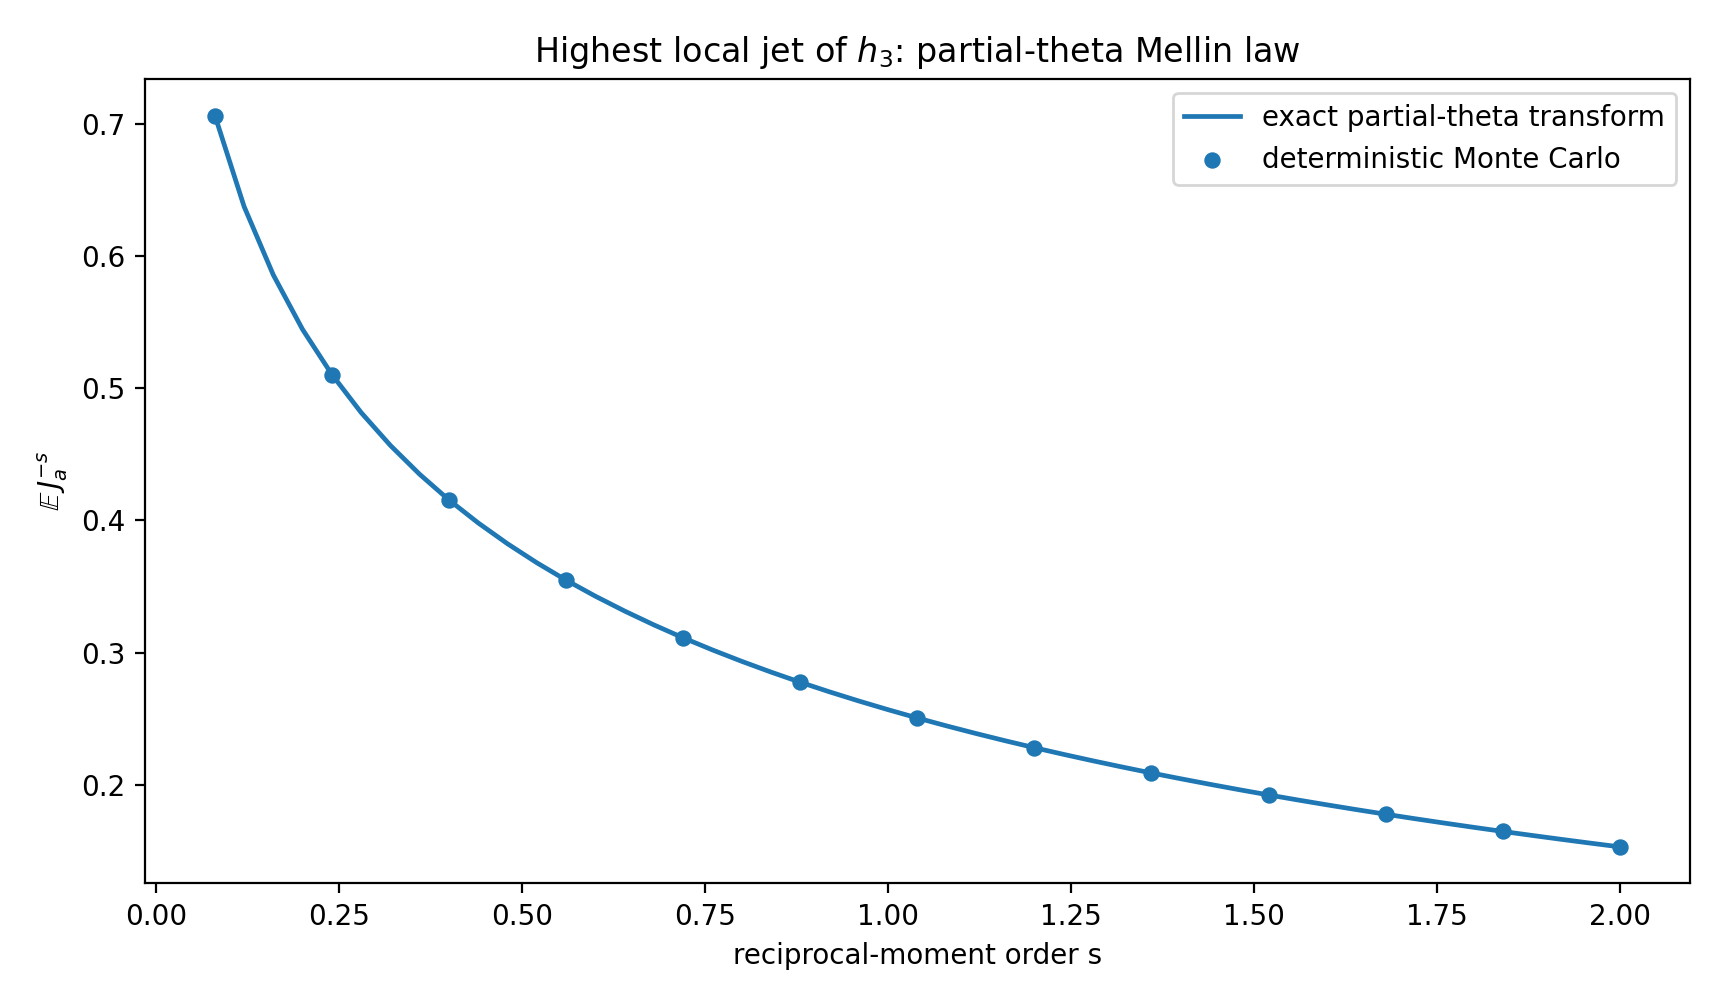
\includegraphics[width=0.88\textwidth]{assets/Atomic_Functions_Rvachev_qBinomial_Frontiers/figures/highest_jet_partial_theta.png}
\caption{The exact reciprocal-moment curve
\eqref{p6:eq:highest-jet-ptheta} at $a=3$ against a fixed-seed simulation
of $1.2\times10^6$ uniform points.}
\label{p6:fig:highest-jet}
\end{figure}

\begin{novelbox}
Two periodic phenomena with the same vertical spacing $2\pi/\log a$ occur in
this part: the complex dimensions \eqref{p6:eq:complex-dimensions} of the gap
string, producing tube oscillations in $\log_a(1/\eps)$, and the Gamma--zeta
Fourier modes of the endpoint Laplace correction in
\cref{p6:sec:general-laplace}, producing endpoint oscillations in $\log_a u$.
They have different amplitudes and arise from different objects---one from the
geometry of $K_a$, one from the law of $X_a$ near its endpoint---but both are
consequences of the same exact multiplicative lattice.  Whether a natural
spectral operator carries one profile into the other is posed in
\cref{p6:sec:future-directions}.
\end{novelbox}

\section{Polynomial reproduction beyond the binary point}

\subsection{Zeros of the Fourier product}

The zeros of $\Phi_a$ are
\begin{equation}\label{p6:eq:Phi-zeros}
 \xi=\frac{k a^j}{2},
 \qquad k\in\Z\setminus\{0\},\quad j\ge1.
\end{equation}
A uniform lattice of translates with spacing $\delta$ reproduces polynomials of
degree $n$ when $\Phi_a$ and its first $n$ derivatives vanish at every nonzero
frequency $m/\delta$.  This is the one-dimensional Strang--Fix mechanism~\cite{p6:strang-fix,p6:deboor-ron}.  The
binary source exploits it in difference-equation form.  For general $a$, zero
collisions are controlled by rational powers of $a$.

\begin{theorem}[Rational-power Strang--Fix theorem]\label{p6:thm:rational-power-SF}
Assume that $a>1$ and that the least positive integer $d$ for which $a^d$ is
rational exists.  Write
\begin{equation}\label{p6:eq:rational-power}
 a^d=\rho=\frac pq,
 \qquad p,q\in\N,\quad p>q,\quad (p,q)=1.
\end{equation}
For a target degree $n\ge0$, define
\begin{equation}\label{p6:eq:lattice-spacing}
 \xi_{a,n}=\frac{ap^n}{2},
 \qquad
 \delta_{a,n}=\xi_{a,n}^{-1}=\frac{2}{ap^n}.
\end{equation}
Then $\Phi_a$ has a zero of multiplicity at least $n+1$ at every nonzero
frequency $m/\delta_{a,n}$.  Consequently every polynomial $P$ of degree at most
$n$ has an exact locally finite representation
\begin{equation}\label{p6:eq:poly-reproduction-general}
 P(x)=\sum_{k\in\Z}c_k(P)
 h_a(x-k\delta_{a,n}),
\end{equation}
where
\begin{equation}\label{p6:eq:poly-coefficients-general}
 c_k(P)=
 \left[
 \delta_{a,n}M_a(\partial_x)^{-1}P
 \right]_{x=k\delta_{a,n}}.
\end{equation}
Because $P$ has finite degree and $M_a(0)=1$, the inverse operator in
\eqref{p6:eq:poly-coefficients-general} is a finite triangular differential
operator on $P$.
\end{theorem}

\begin{proof}
For $\ell=0,1,\ldots,n$, inspect the product factor with index
$j=1+\ell d$.  At $\xi=\xi_{a,n}$,
\[
 2\xi_{a,n}a^{-j}
 =p^na^{-\ell d}
 =p^{n-\ell}q^\ell\in\N.
\]
Hence each of these $n+1$ distinct sinc factors vanishes.  The same is true at
$m\xi_{a,n}$ for every nonzero integer $m$, proving the multiplicity claim.

Let $r\le n$ and periodize $x^rh_a(x)$ with period $\delta=\delta_{a,n}$.
Poisson summation gives Fourier coefficients proportional to derivatives of
$\Phi_a$ at $m/\delta$.  Every nonzero Fourier coefficient vanishes by the
multiplicity just proved, while the zero coefficient is the moment
$m_r(a)/\delta$.  Thus
\begin{equation}\label{p6:eq:periodized-moments}
 \sum_{k\in\Z}(x-k\delta)^r h_a(x-k\delta)
 =\frac{m_r(a)}{\delta},
 \qquad 0\le r\le n.
\end{equation}
For a polynomial $p$ of degree at most $n$, expand
$p(k\delta)=p(x-(x-k\delta))$ and use
\eqref{p6:eq:periodized-moments}:
\begin{align*}
 \sum_{k\in\Z}p(k\delta)h_a(x-k\delta)
 &=\frac1\delta
 \sum_{r=0}^{n}\frac{(-1)^rm_r(a)}{r!}p^{(r)}(x)\\
 &=\frac1\delta M_a(-\partial_x)p(x).
\end{align*}
Here $\partial_x=\dd/\dd x$ is the ordinary derivative (not the
Fourier-normalized symbol $\DF$ used in \cref{p6:eq:atomic-general}).  The law is
symmetric, so $M_a(-\partial_x)=M_a(\partial_x)$.  Choosing
$p=\delta M_a(\partial_x)^{-1}P$ proves the representation.
\end{proof}

\begin{novelbox}
The theorem extends the source's polynomial reproduction from the single binary
point to every parameter whose multiplicative orbit meets the rationals.  The
result is not merely existential: the coefficient polynomial is obtained by
applying the reciprocal moment-generating operator, whose coefficients are the
same Bernoulli--Bell quantities derived in \cref{p6:sec:cumulants}.
\end{novelbox}

\subsection{Explicit low-degree coefficient sequences}

Let $\delta=\delta_{a,n}$.  Since the law is centered,
\[
 M_a(\partial_x)=1+\frac{m_2(a)}{2}\partial_x^2+\frac{m_4(a)}{24}\partial_x^4+\cdots.
\]
Thus the first reproducing sequences are
\begin{align}
 P(x)=1:&\qquad c_k=\delta,\label{p6:eq:reproduce-1}\\
 P(x)=x:&\qquad c_k=\delta(k\delta),\label{p6:eq:reproduce-x}\\
 P(x)=x^2:&\qquad
 c_k=\delta\left((k\delta)^2-m_2(a)\right),\label{p6:eq:reproduce-x2}\\
 P(x)=x^3:&\qquad
 c_k=\delta\left((k\delta)^3-3m_2(a)k\delta\right).
 \label{p6:eq:reproduce-x3}
\end{align}
For degree four,
\begin{equation}\label{p6:eq:reproduce-x4}
 c_k=\delta\left((k\delta)^4-6m_2(a)(k\delta)^2
 +6m_2(a)^2-m_4(a)\right).
\end{equation}
These are Appell-type inverse-moment polynomials.

\begin{example}[Integer parameters]
If $a=A\in\N$, then $d=1$, $p=A$, and
\begin{equation}\label{p6:eq:integer-lattice}
 \delta_{A,n}=\frac{2}{A^{n+1}}.
\end{equation}
At $A=2$, this is exactly the source lattice $2^{-n}$.  At $A=3$, quadratic
reproduction uses spacing $2/27$, while the compact support has width one; each
$x$ therefore sees only finitely many of the coefficient terms.
\end{example}

\begin{example}[A nonrational parameter with a rational power]
For $a=\sqrt2$, take $d=2$, $p=2$, $q=1$.  Degree $n$ reproduction is available
on the lattice
\[
 \delta_{\sqrt2,n}=\frac{2}{\sqrt2\,2^n}=2^{1/2-n}.
\]
The repeated Fourier zeros come from the factors with odd indices
$1,3,5,\ldots,2n+1$.
\end{example}

\subsection{What fails without rational power relations}

If no positive power of $a$ is rational, two distinct sinc factors cannot share
a nonzero zero: equality
$ka^j/2=\ell a^r/2$ would force $a^{j-r}=\ell/k\in\Q$.  Hence every nonzero
zero of $\Phi_a$ is simple.

\begin{conjbox}
\textbf{Uniform-lattice obstruction.}
Suppose $a>1$ has no positive rational power.  Under the usual local stability
or tempered-growth hypotheses on the coefficient sequence, no scalar uniform
lattice of shifts of $h_a$ reproduces every affine polynomial.  Equivalently,
the absence of repeated Fourier zeros is not only a failure of the standard
Strang--Fix construction but a genuine obstruction to all stable one-generator
uniform-lattice reproduction.
\end{conjbox}

A proof should formulate the minimal necessity theorem appropriate to compactly
supported $C^\infty$ generators and locally finite, polynomial-growth
coefficients.  Multi-generator schemes may evade the obstruction and form a
separate research direction.

\section{Fourier decay and smoothness}

\subsection{An elementary log-Gaussian envelope}

Let $t=2\pi|\xi|$ and, for $t\ge a$, put
\[
 N=\lfloor\log_a t\rfloor.
\]
For $1\le j\le N$, the elementary estimate
$|\sinc(t a^{-j})|\le a^j/t$ gives
\begin{equation}\label{p6:eq:Fourier-elementary-bound}
 |\Phi_a(\xi)|
 \le a^{N(N+1)/2}t^{-N}.
\end{equation}
Consequently,
\begin{equation}\label{p6:eq:Fourier-logGaussian}
 \log|\Phi_a(\xi)|
 \le-\frac{(\log t)^2}{2\log a}+\bigO(\log t).
\end{equation}
The bound is faster than every negative power of $|\xi|$, so the compactly
supported density is $C^\infty$.

\begin{remark}
For $a=2$, the repository contains substantially sharper binary estimates and
periodic refinements.  The point of \eqref{p6:eq:Fourier-logGaussian} is its
uniformly transparent dependence on $a$: it already displays the quadratic
logarithmic exponent and is sufficient for all fixed-order Fourier inversions
used below.
\end{remark}

\begin{figure}[H]
\centering
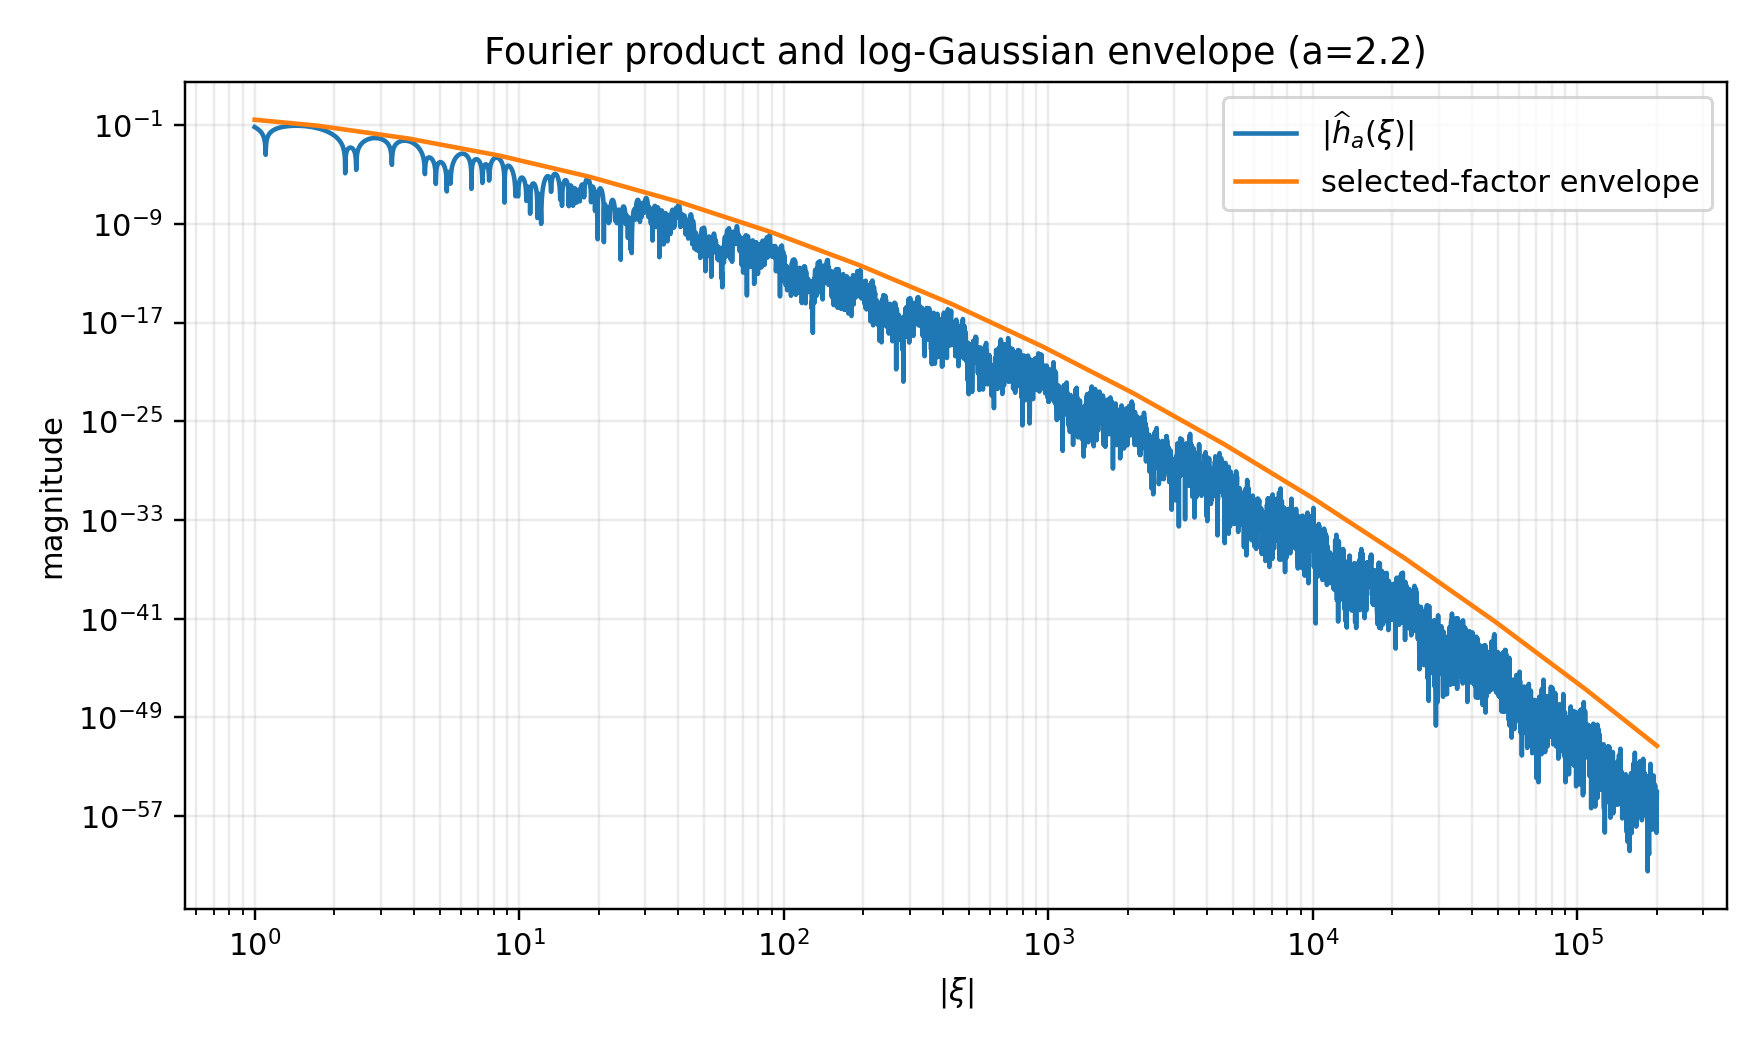
\includegraphics[width=0.94\textwidth]{assets/atomic_sinc_splines_report_package/figures/fourier_envelope_a22.png}
\caption{The Fourier product for $a=2.2$ and the selected-factor bound
\eqref{p6:eq:Fourier-elementary-bound}.  The oscillatory zeros sit well below the
envelope, while the quadratic decay in $\log|\xi|$ is clearly visible.}
\label{p6:fig:fourier-envelope}
\end{figure}

\subsection{Derivative growth from Fourier decay and from self-similarity}

Fourier inversion and \eqref{p6:eq:Fourier-logGaussian} imply a rough
Gevrey-like estimate of the form
\[
 \|h_a^{(r)}\|_\infty
 \le\exp\!\left(\frac{\log a}{2}r^2+\bigO_a(r\log r)\right).
\]
For $a\ge2$, \cref{p6:thm:exact-derivative-norm} is exact and stronger.  The two
proofs illuminate different structures: the Fourier argument survives for all
$a>1$, including overlapping cylinders, whereas the exact norm depends on
separation at $a\ge2$.

\section{Ordinary finite sinc products: an all-orders convergence expansion}

\subsection{Prefix splines and exact tail scaling}

The finite spline $h_{a,N}$ from \eqref{p6:eq:Phi-a-N} is the most literal
piecewise-polynomial approximation to $h_a$.  Its tail is exactly a scaled copy
of the full law:
\[
 X_a=X_{a,N}+a^{-N}X_a',
\]
which gave the convolution identity \eqref{p6:eq:tail-convolution}.  On the Fourier
side,
\begin{equation}\label{p6:eq:prefix-ratio}
 \Phi_{a,N}(\xi)
 =\frac{\Phi_a(\xi)}{\Phi_a(a^{-N}\xi)}.
\end{equation}
This identity turns approximation of $h_a$ into a small-argument expansion of
the reciprocal moment generating function.

Define
\begin{equation}\label{p6:eq:Ra}
 R_a(z)=\frac1{M_a(z)}
 =\sum_{m=0}^{\infty}r_m(a)z^{2m}.
\end{equation}
By \eqref{p6:eq:logMa},
\begin{equation}\label{p6:eq:logRa}
 \log R_a(z)=
 -\sum_{m=1}^{\infty}
 \frac{2^{2m-1}B_{2m}}
 {m(2m)!\,(a^{2m}-1)}z^{2m}.
\end{equation}
In particular,
\begin{align}
 r_0(a)&=1,\label{p6:eq:r0}\\
 r_1(a)&=-\frac1{6(a^2-1)},\label{p6:eq:r1}\\
 r_2(a)&=\frac1{72(a^2-1)^2}
 +\frac1{180(a^4-1)}
 =\frac{7a^2+3}{360(a^2-1)^2(a^2+1)}.
 \label{p6:eq:r2}
\end{align}

\begin{theorem}[All-orders prefix expansion]\label{p6:thm:prefix-expansion}
Fix $a>1$, derivative order $r\ge0$, and truncation order $M\ge1$.  Then, as
$N\to\infty$,
\begin{equation}\label{p6:eq:prefix-expansion}
 h_{a,N}^{(r)}
 =\sum_{m=0}^{M-1}
 r_m(a)a^{-2mN}h_a^{(r+2m)}
 +\bigO_{a,r,M}(a^{-2MN})
\end{equation}
uniformly on $\R$.
\end{theorem}

\begin{proof}
By evenness,
$\Phi_a(\eta)=M_a(2\pi\ii\eta)$.  Thus
\eqref{p6:eq:prefix-ratio} is
\[
 \Phi_{a,N}(\xi)=
 \Phi_a(\xi)R_a(2\pi\ii a^{-N}\xi).
\]
On $|\xi|\le c a^N$, Taylor's theorem for the analytic function $R_a$ gives a
remainder bounded by
$C a^{-2MN}|\xi|^{2M}$.  Multiplication by
$(2\pi\ii\xi)^r\Phi_a(\xi)$ is integrable by
\eqref{p6:eq:Fourier-logGaussian}.  On the complementary frequencies, both the
full product and the $N$-factor product have a bound of order
$\exp(-c_aN^2)$ after choosing $c$ below the first reciprocal zero.  This is
smaller than $a^{-2MN}$ for fixed $M$.  Fourier inversion proves the uniform
expansion.
\end{proof}

\begin{corollary}[First correction]\label{p6:cor:first-prefix-correction}
For every fixed $r\ge0$,
\begin{equation}\label{p6:eq:first-prefix-correction}
 a^{2N}\bigl(h_{a,N}^{(r)}-h_a^{(r)}\bigr)
 \longrightarrow
 -\frac{h_a^{(r+2)}}{6(a^2-1)}
\end{equation}
uniformly on $\R$.
\end{corollary}

\begin{corollary}[Exact leading norm for $a\ge2$]\label{p6:cor:prefix-norm}
For $a\ge2$,
\begin{equation}\label{p6:eq:prefix-norm-leading}
 a^{2N}\|h_{a,N}-h_a\|_\infty
 \longrightarrow
 \frac{a^6}{48(a^2-1)}.
\end{equation}
More generally,
\begin{equation}\label{p6:eq:prefix-derivative-norm-leading}
 a^{2N}\|h_{a,N}^{(r)}-h_a^{(r)}\|_\infty
 \longrightarrow
 \frac{1}{6(a^2-1)}
 \frac{a^{(r+2)(r+5)/2+1}}{2^{r+3}}.
\end{equation}
\end{corollary}

\begin{proof}
Combine \cref{p6:cor:first-prefix-correction} with the exact derivative norm
\eqref{p6:eq:exact-derivative-norm-closed}.
\end{proof}

\begin{novelbox}
The sign of the first correction is important.  The ordinary Fourier-prefix
spline has leading profile $-h_a''/[6(a^2-1)]$.  The current repository also
studies a different finite approximation produced by repeated integration and
support correction; its leading binary coefficient is positive.  The two
schemes should not be identified: they invert different finite operators and
therefore have different asymptotic signatures.
\end{novelbox}

\begin{figure}[H]
\centering
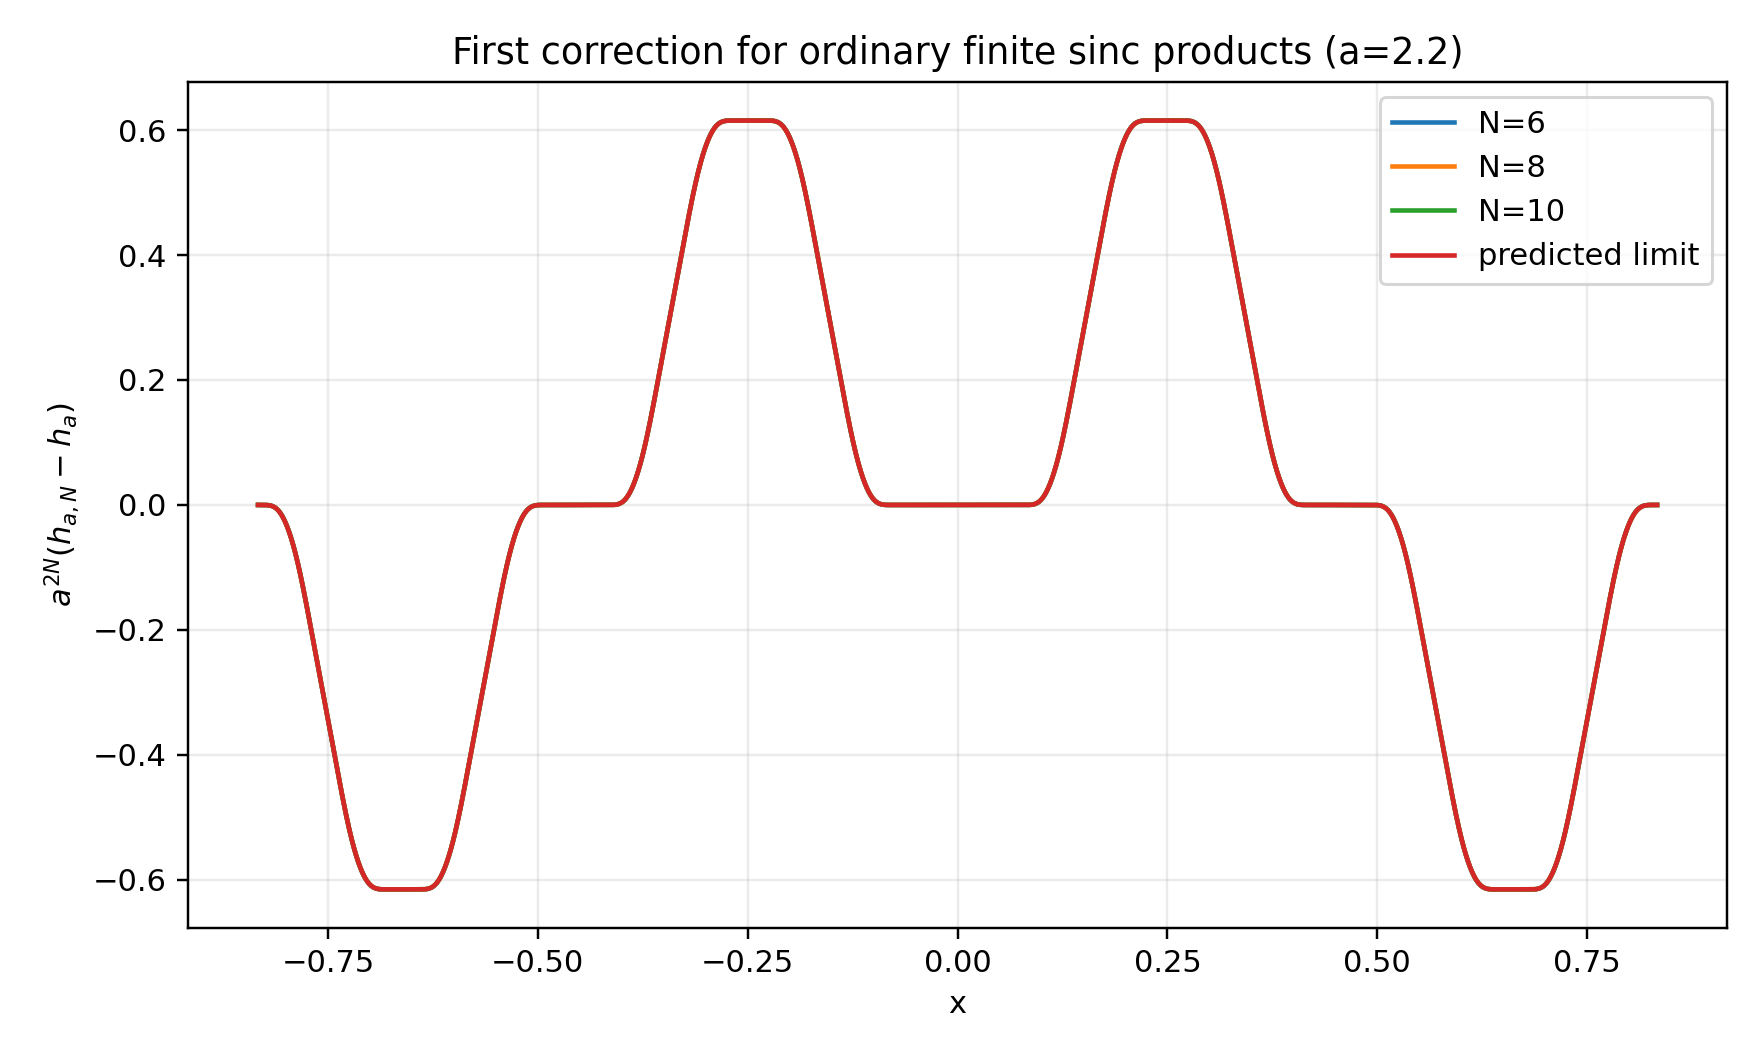
\includegraphics[width=0.94\textwidth]{assets/atomic_sinc_splines_report_package/figures/scaled_prefix_error_a22.png}
\caption{For $a=2.2$, the scaled errors
$a^{2N}(h_{a,N}-h_a)$ for $N=6,8,10$ are visually indistinguishable from
$-h_a''/[6(a^2-1)]$.  The computation uses FFT inversion of the explicit
products, not random sampling.}
\label{p6:fig:prefix-correction}
\end{figure}

\subsection{Interpretation as an inverse approximate identity}

The convolution relation $h_a=h_{a,N}*g_N$, where
$g_N(x)=a^Nh_a(a^Nx)$, is an approximate-identity statement in the direction
$h_{a,N}\mapsto h_a$.  Recovering $h_{a,N}$ from $h_a$ is therefore a formal
deconvolution.  The reciprocal series $R_a$ is exactly the inverse of the tail
moment operator.  This explains why the coefficients are not raw moments but
inverse Bell polynomials in the cumulants.

\section{The critical deformation \texorpdfstring{$a\downarrow2$}{a down to 2}}

\subsection{A deterministic coupling bound}

Use the same uniform variables in the definitions of $X_a$ and $X_2$.  For
$a>2$,
\begin{equation}\label{p6:eq:coupling-bound}
 |X_a-X_2|
 \le\sum_{j=1}^{\infty}(2^{-j}-a^{-j})
 =1-\frac1{a-1}
 =\frac{a-2}{a-1}.
\end{equation}
Thus the $L^\infty$ Wasserstein distance satisfies
\begin{equation}\label{p6:eq:Winfty}
 W_\infty(\mathcal L(X_a),\mathcal L(X_2))
 \le\frac{a-2}{a-1}.
\end{equation}
If $H_a$ denotes the CDF of $X_a$, the coupling immediately gives the bracket
\begin{equation}\label{p6:eq:CDF-bracket}
 H_2(x-\eta_a)\le H_a(x)\le H_2(x+\eta_a),
 \qquad \eta_a=\frac{a-2}{a-1}.
\end{equation}

\begin{proposition}[$C^r$ convergence to $\Up$]\label{p6:prop:C-r-to-up}
For every fixed $r\ge0$,
\begin{equation}\label{p6:eq:C-r-convergence}
 h_a\longrightarrow\Up
 \quad\text{in }C^r(\R)
 \qquad(a\downarrow2).
\end{equation}
\end{proposition}

\begin{proof}
The Fourier products converge pointwise to the binary product.  For
$a\in[2,2+\varepsilon]$, the log-Gaussian bound
\eqref{p6:eq:Fourier-logGaussian} may be chosen with one integrable majorant after
multiplication by any fixed power $|\xi|^r$.  Dominated convergence in Fourier
inversion gives the result.
\end{proof}

\subsection{Collapse of the fractal spline geometry}

As $a=2+\varepsilon\downarrow2$,
\begin{align}
 b_1&=\frac{a-2}{a(a-1)}
 =\frac\varepsilon2+\bigO(\varepsilon^2),\label{p6:eq:gap-collapse}\\
 \dim_{\mathrm H}K_a&=\frac{\log2}{\log(2+\varepsilon)}
 =1-\frac{\varepsilon}{2\log2}+\bigO(\varepsilon^2).
 \label{p6:eq:dimension-collapse}
\end{align}
The full-measure polynomial-gap set therefore degenerates in a singular way:
individual gaps shrink, their exceptional complement increases in dimension to
one, and the limiting $\Up$ is nowhere analytic.

\begin{conjbox}
\textbf{Critical boundary-layer scaling.}
There is a nontrivial double-scaling limit in which
$a=2+\varepsilon$, the gap depth $r$ tends to infinity, and
$r\varepsilon$ remains bounded.  After centering at an endpoint of a depth-$r$
gap and rescaling by its width $a^{-r}b_1$, the polynomial pieces should converge
to universal profiles governed by the binary $\Up$ derivative hierarchy.
\end{conjbox}

\begin{figure}[H]
\centering
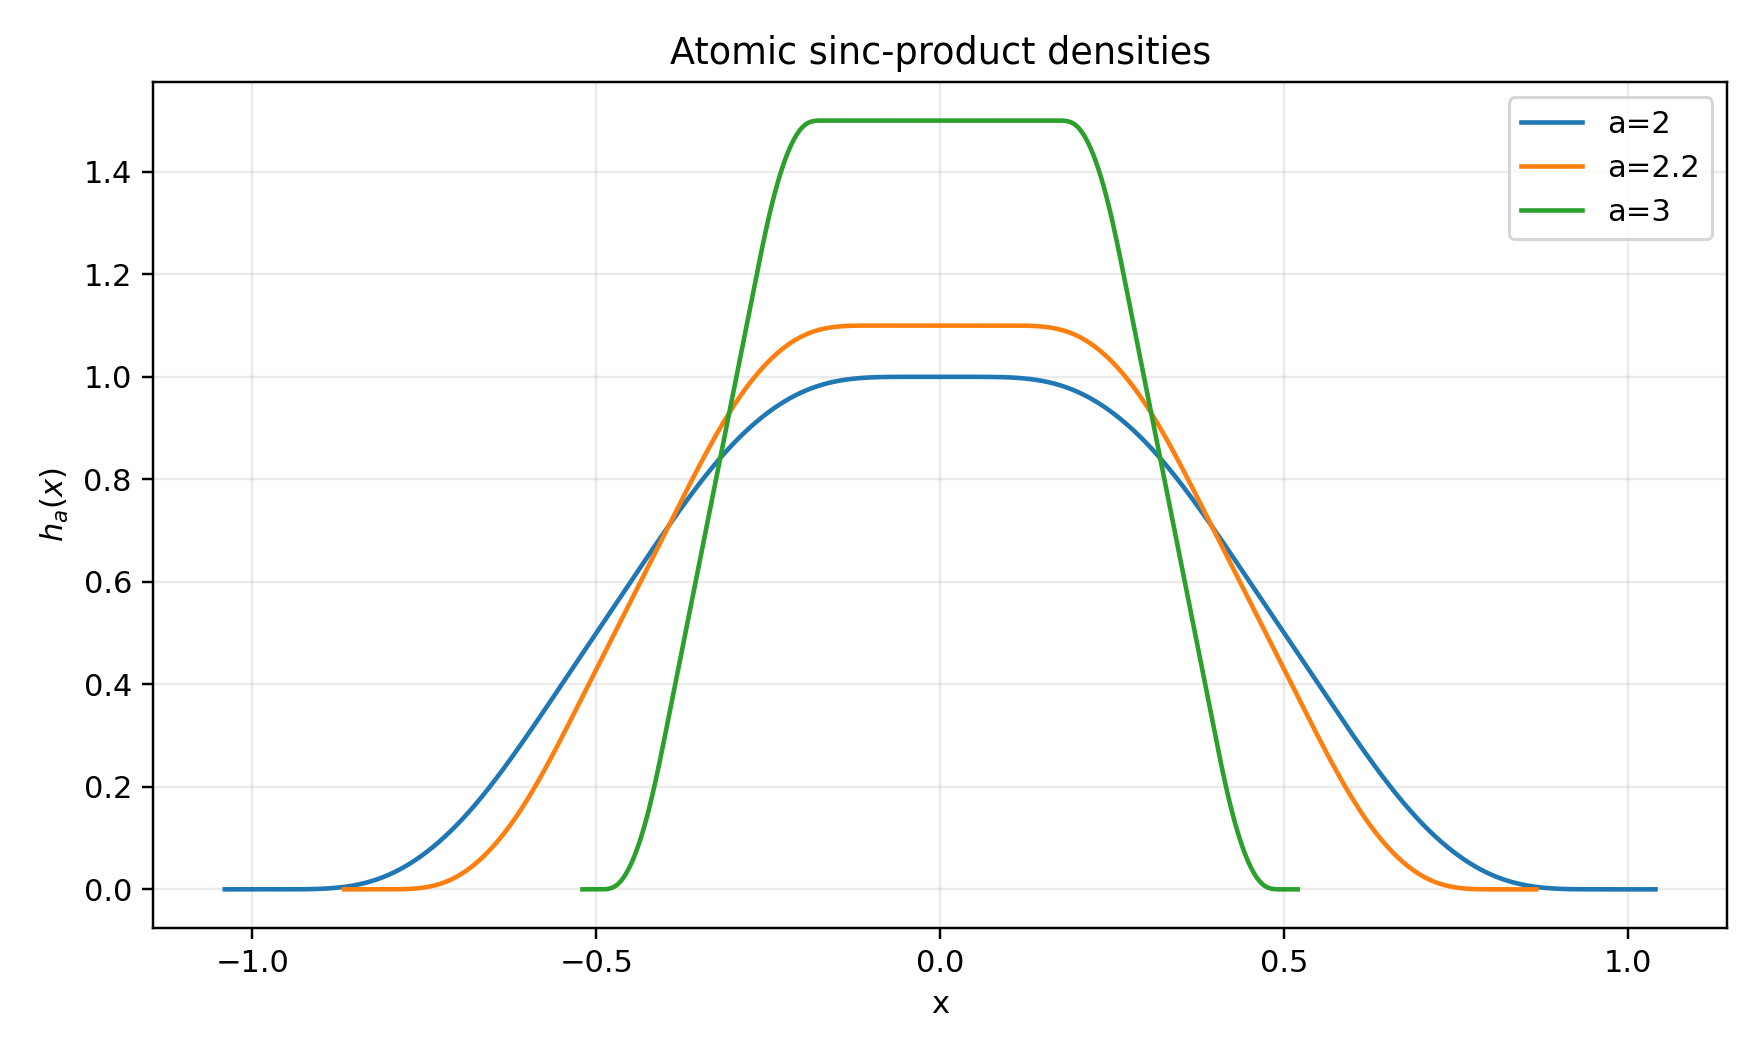
\includegraphics[width=0.94\textwidth]{assets/atomic_sinc_splines_report_package/figures/family_profiles.png}
\caption{Profiles of $h_a$ at the critical point $a=2$ and in the separated
regime.  The central plateau has height $a/2$ and half-width
$(a-2)/(a(a-1))$ for $a>2$; it collapses to the single maximum of $\Up$ at
$a=2$.}
\label{p6:fig:family-profiles}
\end{figure}

\section{Parameter limits: the Gaussian and uniform ends of the family}
\label{p6:sec:parameter-limits}

The previous section treats the critical deformation $a\downarrow2$.  This
section (fourteenth wave) settles the two extreme ends of the parameter range,
completing the limit atlas of the family: normalized Gaussian behavior as
$a\downarrow1$, exact uniform behavior as $a\to\infty$, and quantitative rates
at both ends.

\subsection{The many-small-summands limit \texorpdfstring{$a\downarrow1$}{a down to 1}}

By \eqref{p6:eq:m2}, the standard deviation is
$\sigma_a=\bigl(3(a^2-1)\bigr)^{-1/2}$; let $Z_a=X_a/\sigma_a$.

\begin{theorem}[Gaussian limit and first characteristic correction]
\label{p6:thm:gaussian-limit}
As $a\downarrow1$,
\begin{equation}\label{p6:eq:gaussian-limit}
 Z_a\ \xrightarrow{\ d\ }\ N(0,1).
\end{equation}
The standardized cumulants are, for $m\ge2$,
\begin{equation}\label{p6:eq:standardized-cumulant}
 \lambda_{2m}(a)
 =\frac{\kappa_{2m}(X_a)}{\sigma_a^{2m}}
 =\frac{3^m2^{2m}B_{2m}\,(a^2-1)^m}{2m\,(a^{2m}-1)}
 =\bigO\bigl((a-1)^{m-1}\bigr),
\end{equation}
with in particular
\begin{equation}\label{p6:eq:lambda4}
 \lambda_4(a)=-\frac65\,\frac{a^2-1}{a^2+1}.
\end{equation}
Consequently, for every fixed $T>0$, uniformly for real $|t|\le T$,
\begin{equation}\label{p6:eq:gaussian-first-correction}
 \E\,\e^{\ii tZ_a}
 =\e^{-t^2/2}
 \left[1-\frac{a^2-1}{20\,(a^2+1)}\,t^4
 +\bigO_T\bigl((a-1)^2\bigr)\right].
\end{equation}
\end{theorem}

\begin{proof}
The triangular array $Z_a=\sum_j\sqrt{3(a^2-1)}\,a^{-j}U_j$ has total variance
one and maximal coefficient tending to zero, so the Lindeberg theorem gives
\eqref{p6:eq:gaussian-limit}.  Formula \eqref{p6:eq:standardized-cumulant} is
\eqref{p6:eq:kappa} divided by $\sigma_a^{2m}$; writing $a=1+\eta$, the ratio
$(a^2-1)^m/(a^{2m}-1)\sim2^{m-1}\eta^{m-1}/m$ gives the order.  Since the
log-characteristic function of $Z_a$ is
$-t^2/2+\lambda_4(a)t^4/4!+\bigO_T((a-1)^2)$ on $|t|\le T$, and
$\lambda_4/4!=-\tfrac{a^2-1}{20(a^2+1)}$, exponentiation gives
\eqref{p6:eq:gaussian-first-correction}.
\end{proof}

\begin{conjbox}
\textbf{Uniform local Edgeworth expansion.}
The characteristic expansion \eqref{p6:eq:gaussian-first-correction} and the
superpolynomial Fourier decay of \cref{p6:eq:Fourier-logGaussian} make an
all-orders local Edgeworth expansion for the normalized densities
$\sigma_ah_a(\sigma_a\,\cdot)$ and their derivatives plausible.  The open
difficulty is uniform control of the large-frequency range as $a\downarrow1$:
in normalized units the envelope \eqref{p6:eq:Fourier-logGaussian} becomes
effective only beyond frequencies of order
$\sigma_a\asymp(a-1)^{-1/2}$, so the central and tail regimes must be split at
a threshold that itself diverges in the joint limit.
\end{conjbox}

\begin{figure}[H]
\centering

\includegraphics[width=0.94\textwidth]{assets/Atomic_Functions_Beyond_Dyadic_Report/figures/gaussian_cumulant_limit.png}
\caption{The exact standardized fourth cumulant \eqref{p6:eq:lambda4} and its
first asymptotic term as $a\downarrow1$.}
\label{p6:fig:gaussian-limit}
\end{figure}

\subsection{The single-dominant-summand limit \texorpdfstring{$a\to\infty$}{a to infinity}}

Rescale by the leading weight: put $Y_a=aX_a=U_1+T_a$ with
$T_a=\sum_{j\ge2}a^{-(j-1)}U_j$, so $|T_a|\le1/(a-1)$ almost surely.

\begin{theorem}[Uniform limit with exact core]\label{p6:thm:uniform-limit}
Let $U\sim\operatorname{Unif}[-1,1]$ and let $g_a(y)=h_a(y/a)/a$ denote the
density of $Y_a$.  For every $a>2$,
\begin{equation}\label{p6:eq:uniform-bounds}
 W_\infty\bigl(\mathcal L(Y_a),\mathcal L(U)\bigr)\le\frac1{a-1},
 \qquad
 d_{\mathrm{TV}}\bigl(\mathcal L(Y_a),\mathcal L(U)\bigr)\le\frac1{2(a-1)},
\end{equation}
and the convergence is exact on an expanding central core:
\begin{equation}\label{p6:eq:uniform-core}
 g_a(y)=\frac12
 \qquad\text{for}\qquad
 |y|\le\frac{a-2}{a-1}.
\end{equation}
All discrepancy is confined to the two boundary layers
$\tfrac{a-2}{a-1}<|y|\le\tfrac{a}{a-1}$, each of width $2/(a-1)$.
\end{theorem}

\begin{proof}
The coupling $Y_a=U_1+T_a$ gives the $W_\infty$ bound.  Conditional on
$T_a=r$, the law of $Y_a$ is uniform on $[r-1,r+1]$, whose total variation
distance from $\operatorname{Unif}[-1,1]$ is $|r|/2$; averaging over $r$ and
convexity of total variation give the second bound.  Finally
$g_a(y)=h_a(y/a)/a$, and the plateau \eqref{p6:eq:plateau} of half-width $b_1$
becomes \eqref{p6:eq:uniform-core} because $ab_1=(a-2)/(a-1)$, with plateau
height $(a/2)/a=1/2$.
\end{proof}

Together with \cref{p6:prop:C-r-to-up}, the family therefore interpolates
between three classical laws with explicit rates: Gaussian after normalization
at $a\downarrow1$, the nowhere-analytic critical atom at $a=2$, and the
single uniform digit after rescaling at $a\to\infty$.

\section{Endpoint tails, inverse Fabius behavior, and Lambert \texorpdfstring{$W$}{W}}
\label{p6:sec:general-laplace}

\subsection{The endpoint random series}

Let
\begin{equation}\label{p6:eq:Ya}
 Y_a=b_a-X_a.
\end{equation}
Writing $V_j=(1-U_j)/2$, with $V_j$ uniform on $[0,1]$, gives
\begin{equation}\label{p6:eq:Ya-series}
 Y_a=2\sum_{j=1}^{\infty}a^{-j}V_j.
\end{equation}
Its Laplace transform is
\begin{equation}\label{p6:eq:Ya-Laplace}
 L_a(s)=\E\e^{-sY_a}
 =\prod_{j=1}^{\infty}
 \frac{1-\e^{-2sa^{-j}}}{2sa^{-j}}.
\end{equation}
For large $s$, roughly the first $\log_a s$ factors contribute
$a^j/(2s)$ and the remaining factors are close to one.  Therefore
\begin{equation}\label{p6:eq:Laplace-log-leading}
 \log L_a(s)
 =-\frac{(\log s)^2}{2\log a}
 +\bigO(\log s),
\end{equation}
with an unavoidable bounded oscillation in the fractional part of $\log_a s$.
This is the same discrete-scale mechanism that produces the periodic correction
in the repository's binary endpoint asymptotics.  The heuristic
\eqref{p6:eq:Laplace-log-leading} is made exact, in every base, in
\cref{p6:thm:general-periodic} below: in the variable $u=2s$, the full
log-Laplace transform is a quadratic-plus-linear polynomial in $\log u$, plus a
real-analytic one-periodic function of $\log_au$, plus an explicit
exponentially small tail, with no error term.

\subsection{Why the lower Lambert branch appears}

A Bromwich or Laplace saddle for the small-$y$ density balances
$sy$ against $-\log L_a(s)$.  Differentiating the leading term gives
\begin{equation}\label{p6:eq:saddle-balance}
 sy\asymp\frac{\log s}{\log a}.
\end{equation}
If $u=\log s$, then $y\e^u\asymp u/\log a$, so
\begin{equation}\label{p6:eq:Lambert-coordinate}
 u\asymp-W_{-1}(-y\log a).
\end{equation}
The lower branch is required because $u\to+\infty$ as $y\downarrow0$; see~\cite{p6:corless} for the branch structure of Lambert $W$.
For $a=2$, this is exactly the coordinate used in the repository's inverse and
small-argument expansions.

\subsection{The edge pantograph equation}

The same structure is visible without any transform (fifteenth wave).  Let
$g_a(u)=h_a(-b_a+u)$ for $0\le u\le2b_a$.  For $0\le u\le2/a$ the branch
$h_a(a(-b_a+u)-1)$ of \eqref{p6:eq:ha-diffeq} lies outside the support, while
$a(-b_a+u)+1=-b_a+au$, so the edge profile solves the pantograph equation
\begin{equation}\label{p6:eq:edge-pantograph}
 g_a'(u)=\frac{a^2}{2}\,g_a(au),
 \qquad 0\le u\le\frac2a,
\end{equation}
and iterating along the flat edge gives the exact identity
\begin{equation}\label{p6:eq:edge-iterated}
 g_a^{(n)}(u)=\frac{a^{n(n+3)/2}}{2^n}\,g_a\bigl(a^nu\bigr),
 \qquad 0\le u\le2a^{-n},
\end{equation}
the endpoint case of the one-branch localization
\eqref{p6:eq:symbolic-localization}.  Normalizing by
$F_a(x)=\tfrac2a\,h_a(-b_a+b_ax)$ produces a generalized Fabius profile with
$F_2=F$ on $[0,1]$ and
\begin{equation}\label{p6:eq:Fa-pantograph}
 F_a'(x)=\frac{a^2}{2(a-1)}\,F_a(ax),
 \qquad 0\le x\le\frac{2(a-1)}{a},
\end{equation}
with $h_a$ extended by zero beyond its support; for $a\ge\tfrac32$ this range
contains $[0,1/a]$, on which the recursion is closed in the unit
normalization, and at $a=2$ it specializes to the repository identity
$F'(x)=2F(2x)$.
Pantograph equations of this type sit alongside de Rham's functional
equations~\cite{p6:derham}, and \eqref{p6:eq:edge-iterated} already forces the
quadratic-in-depth exponents whose inversion is Lambert-$W$; the following
subsections make that heuristic exact at the transform level.

\subsection{The exact periodic decomposition in every base}

The heuristics above are now made exact (fourteenth wave).  For $u>0$, put
\begin{equation}\label{p6:eq:kernel-varkappa}
 \varkappa(u)=\log\frac{1-\e^{-u}}{u},
 \qquad
 \Lambda_a(u)=\sum_{j=1}^{\infty}\varkappa\bigl(ua^{-j}\bigr),
\end{equation}
so that $\log L_a(s)=\Lambda_a(2s)$ by \eqref{p6:eq:Ya-Laplace}.  The kernel
$\varkappa$ is exactly the kernel of the binary Mellin reflection theory of
Part~I (\cref{p1:thm:mellin-reflection}); here it is summed over a single
geometric orbit in an arbitrary base.  Termwise,
\begin{equation}\label{p6:eq:Lambda-dilation}
 \Lambda_a(au)=\Lambda_a(u)+\varkappa(u).
\end{equation}
Define the exponentially convergent, nonnegative tail sum
\begin{equation}\label{p6:eq:Ea-def}
 E_a(u)=\sum_{n=0}^{\infty}-\log\bigl(1-\e^{-ua^{n}}\bigr)\ \ge0,
 \qquad u>0,
\end{equation}
and put
\begin{equation}\label{p6:eq:Pa-def}
 P_a(x)=\Lambda_a(a^x)+\frac{\log a}{2}\,x^2-\frac{\log a}{2}\,x-E_a(a^x).
\end{equation}

\begin{theorem}[General-base exact periodic decomposition]
\label{p6:thm:general-periodic}
For every $a>1$, the function $P_a$ is one-periodic, and for every $u>0$,
\begin{equation}\label{p6:eq:general-exact-Laplace}
 \Lambda_a(u)=
 -\frac{(\log u)^2}{2\log a}+\frac{\log u}{2}
 +P_a\bigl(\log_au\bigr)+E_a(u),
\end{equation}
with
\begin{equation}\label{p6:eq:Ea-bound}
 0\le E_a(u)\le
 \frac{\e^{-u}}{(1-\e^{-u})\bigl(1-\e^{-(a-1)u}\bigr)}
 =\bigO_a(\e^{-u})
 \qquad(u\to\infty).
\end{equation}
\end{theorem}

\begin{proof}
Dropping the $n=0$ term in \eqref{p6:eq:Ea-def} gives
$E_a(a^{x+1})=E_a(a^x)+\log(1-\e^{-a^x})$, while
$\varkappa(a^x)=\log(1-\e^{-a^x})-x\log a$.  With the dilation identity
\eqref{p6:eq:Lambda-dilation},
\[
 P_a(x+1)-P_a(x)
 =\varkappa(a^x)+x\log a
 -\bigl(E_a(a^{x+1})-E_a(a^x)\bigr)=0,
\]
so $P_a$ is one-periodic.  Rearranging \eqref{p6:eq:Pa-def} at $x=\log_au$
gives \eqref{p6:eq:general-exact-Laplace}.  For the tail bound, use
$-\log(1-z)\le z/(1-z)$ for $0<z<1$ and $a^n\ge1+n(a-1)$, then sum the
resulting geometric series.
\end{proof}

At $a=2$, the bound \eqref{p6:eq:Ea-bound} becomes
$E_2(u)\le\e^{-u}/(1-\e^{-u})^2$, exactly the tail form in the repository's
primary binary exposition; \cref{p6:thm:general-periodic} is thus a base-$a$
renormalization of the same mechanism, not an analogy.

\subsection{Gamma--zeta Fourier modes of the periodic term}

Let
\begin{equation}\label{p6:eq:Psi-a}
 \overline P_a=\int_0^1P_a(x)\,\dd x,
 \qquad
 \Psi_a=P_a-\overline P_a,
 \qquad
 \chi_k=\frac{2\pi\ii k}{\log a}.
\end{equation}

\begin{theorem}[General-base Gamma--zeta modes]
\label{p6:thm:general-fourier-modes}
For every $a>1$ and every $k\ne0$,
\begin{equation}\label{p6:eq:general-gamma-zeta}
 \widehat\Psi_a(k)=\int_0^1\Psi_a(x)\,\e^{-2\pi\ii kx}\dd x
 =-\frac{\Gamma(-\chi_k)\,\zeta(1-\chi_k)}{\log a}.
\end{equation}
The coefficients decay exponentially in $|k|$, so $P_a$ is real analytic; and
every nonzero mode is nonzero, so $P_a$ is nonconstant.
\end{theorem}

\begin{proof}[Proof sketch]
On the strip $-1<\Re s<0$, the kernel transform is
$\int_0^\infty\varkappa(u)u^{s-1}\dd u=-\Gamma(s)\zeta(s+1)$
(\cref{p1:thm:mellin-reflection}, there for the same kernel).  The harmonic sum
$\Lambda_a(u)=\sum_{j\ge1}\varkappa(ua^{-j})$ therefore has Mellin transform
$-\Gamma(s)\zeta(s+1)\,a^{s}/(1-a^{s})$ on the same strip, and Mellin inversion
with the contour pushed across $\Re s=0$ produces: the quadratic and linear
terms of \eqref{p6:eq:general-exact-Laplace} from the triple pole at $s=0$; the
lattice modes from the simple poles of $1/(1-a^s)$ at $s=\chi_k$, whose
residues sample the kernel transform at $s=-\chi_k$ after pairing $k\to-k$,
giving \eqref{p6:eq:general-gamma-zeta}; and a remainder absorbed by
$E_a$~\cite{p6:flajolet-gd}.  Stirling's bound
$|\Gamma(\sigma+\ii t)|\asymp\e^{-\pi|t|/2}|t|^{\sigma-1/2}$ gives exponential
decay in $|k|$.  Since $\Gamma$ has no zeros and $\zeta(1+\ii t)\ne0$ for
$t\ne0$, every mode \eqref{p6:eq:general-gamma-zeta} is nonzero.
\end{proof}

\begin{figure}[H]
\centering

\includegraphics[width=0.94\textwidth]{assets/Atomic_Functions_Beyond_Dyadic_Report/figures/periodic_correction_bases.png}
\caption{Centered periodic corrections $\Psi_a=P_a-\overline P_a$ for several
bases.  The dyadic oscillation has amplitude of order $10^{-6}$; the amplitude
grows substantially with the base, following the mode formula
\eqref{p6:eq:general-gamma-zeta}.}
\label{p6:fig:periodic-correction}
\end{figure}

\begin{repobox}
At $a=2$, the mode lattice $\chi_k=2\pi\ii k/\log2$ is precisely the vertical
lattice of the repository's binary endpoint theory, and Part~I's reflection
formula \eqref{p1:eq:mellin-reflection} is the composite-scale refinement in
which an additional spectral factor $A(2^w)$ multiplies the same
$\Gamma$--$\zeta$ kernel transform.  The theorem above is the single-scale,
arbitrary-base member of that family.  Note also the second appearance of the
lattice $2\pi\ii k/\log a$ in this part: the complex dimensions
\eqref{p6:eq:complex-dimensions} of the gap string share the vertical spacing
but not the amplitudes.
\end{repobox}

\subsection{The exact saddle and the general-base lower-Lambert coordinate}

The decomposition also pins the saddle coordinate.  The exact saddle equation
for the endpoint density at depth $y$ is
\begin{equation}\label{p6:eq:exact-saddle}
 y+2\Lambda_a'\bigl(2s_a(y)\bigr)=0.
\end{equation}
Differentiating \eqref{p6:eq:general-exact-Laplace},
\[
 y\,s=\log_a(2s)-\tfrac12-\frac{P_a'\bigl(\log_a2s\bigr)}{\log a}
 -2s\,E_a'(2s),
\]
so, ignoring the bounded periodic derivative and the exponentially small tail,
the variable $\rho=\log_a\bigl(2s/\sqrt a\bigr)$ satisfies
\begin{equation}\label{p6:eq:r-Lambert-equation}
 \rho\,a^{-\rho}=\frac{y\sqrt a}{2},
\end{equation}
whose large solution is the general-base lower-Lambert coordinate
\begin{equation}\label{p6:eq:r-Lambert}
 r_a(y)=-\frac1{\log a}
 W_{-1}\!\left(-\frac{y\sqrt a\,\log a}{2}\right)
 \longrightarrow\infty
 \qquad(y\downarrow0).
\end{equation}
The half-unit shift hidden in $\sqrt a$ is exactly the linear term
$+\tfrac12\log u$ of the decomposition; at $a=2$, this normalization matches
the repository's binary inverse coordinate.

\begin{conjbox}
\textbf{All-orders endpoint expansion for $h_a$ (refined).}
Let $\delta\downarrow0$ and
$U_a(\delta)=-W_{-1}(-c_a\delta)$ for a normalization constant $c_a>0$.
There exist smooth $1$-periodic coefficient functions
$\Psi_{a,j}$ such that
\begin{equation}\label{p6:eq:endpoint-conjecture}
 \log h_a(-b_a+\delta)
 \sim-\frac{U_a(\delta)^2}{2\log a}
 +A_aU_a(\delta)+B_a\log U_a(\delta)
 +\sum_{j\ge0}\frac{
 \Psi_{a,j}(\{U_a(\delta)/\log a\})}
 {U_a(\delta)^j}.
\end{equation}
The periodic phase records the exact position of the saddle between neighboring
geometric scales.  An analogous expansion should hold for the CDF and for the
inverse of the affine $q$-CDF.  At $a=2$, after normalization, it must reduce to
the existing binary expansion in the repository.
\end{conjbox}

% ed.: the transform-level half of this program is now closed by
% \cref{p6:thm:general-periodic,p6:thm:general-fourier-modes} (fourteenth wave);
% the closing task list below is updated accordingly.
Of the tasks formerly open here, the identification of the normalization
$c_a=\sqrt a\,\log a/2$ and of the leading-order constants, and the construction
of the periodic phase, are settled at the transform level by
\eqref{p6:eq:r-Lambert} and
\cref{p6:thm:general-periodic,p6:thm:general-fourier-modes}: the order-one
oscillation of the conjectured expansion must be $\Psi_a$ evaluated at the
saddle phase, with the saddle jets generated by the derivatives of $P_a$.  What
remains open is the density level: existence and uniqueness of the exact saddle
\eqref{p6:eq:exact-saddle} for small $y$, the steepest-descent contour with a
uniform remainder, and uniformity of all constants for $a$ in compact subsets
of $(1,\infty)$.

\section{Deterministic numerical experiments}

\subsection{Reproducibility design}

The supplied program \texttt{numerics.py} uses three independent modes of
verification.
\begin{enumerate}
\item \textbf{Exact rational arithmetic.}  SymPy evaluates Bernoulli numbers,
cumulants, and moments as exact fractions.  The weighted Prouhet sums are
computed as Python integers.
\item \textbf{Direct Fourier inversion.}  Densities and derivatives are obtained
from the explicit sinc products on a zero-padded FFT grid.  The computational
box is wider than the compact support, so periodic copies do not overlap.
\item \textbf{Profile-level asymptotics.}  The scaled function
$a^{2N}(h_{a,N}-h_a)$ is compared pointwise with
$-h_a''/[6(a^2-1)]$, not merely through a single fitted scalar.
\end{enumerate}
No Monte Carlo simulation is used.  The exact identities remain valid
independently of the numerical section.

\subsection{Exact moment table}

The following sample is generated from \eqref{p6:eq:moment-recurrence}; the full
CSV includes even moments through order twelve for $a=2$, $11/5$, and $3$.
\begin{table}[H]
\centering
\small
\begin{tabular}{@{}ccl@{}}
\toprule
$a$ & order & exact moment \\
\midrule
$2$ & $2$ & $1/9$ \\
$2$ & $4$ & $19/675$ \\
$2$ & $6$ & $583/59535$ \\
$2$ & $8$ & $132809/32531625$ \\
$11/5$ & $2$ & $25/288$ \\
$11/5$ & $4$ & $33625/2018304$ \\
$3$ & $2$ & $1/24$ \\
$3$ & $4$ & $17/4800$ \\
\bottomrule
\end{tabular}
\caption{Selected exact moments from \texttt{data/moments.csv}.}
\label{p6:tab:moments}
\end{table}

\subsection{Weighted Prouhet checks}

For $a=2,3$ and $1\le n\le8$, the program enumerates all $2^n$ sign vectors and
checks
\[
 \sum_{\boldsymbol\varepsilon}w(\boldsymbol\varepsilon)
 s_a(\boldsymbol\varepsilon)^m
 =\begin{cases}
 0,&m<n,\\
 2^nn!a^{n(n-1)/2},&m=n.
 \end{cases}
\]
Every row in \texttt{data/prouhet\_checks.csv} is marked
\texttt{True}.  For example, the largest check is
\[
 \sum_{\boldsymbol\varepsilon\in\{\pm1\}^8}
 w(\boldsymbol\varepsilon)s_3(\boldsymbol\varepsilon)^8
 =236132421576711045120.
\]

\subsection{Prefix-spline convergence}

The leading norm constants predicted by \eqref{p6:eq:prefix-norm-leading} are
\begin{equation}\label{p6:eq:numeric-limit-constants}
 \frac49\quad(a=2),
 \qquad
 0.615125347222\ldots\quad(a=2.2),
 \qquad
 \frac{243}{128}=1.8984375\quad(a=3).
\end{equation}
The FFT calculations give the following scaled errors.
\begin{table}[H]
\centering
\small
\begin{tabular}{@{}cccc@{}}
\toprule
$a$ & $N$ & $a^{2N}\|h_{a,N}-h_a\|_\infty$ & predicted limit \\
\midrule
$2$ & $4$ & $0.4444444444445$ & $0.4444444444444$ \\
$2$ & $8$ & $0.4444444444598$ & $0.4444444444444$ \\
$2.2$ & $4$ & $0.6151253472224$ & $0.6151253472222$ \\
$2.2$ & $8$ & $0.6151253473366$ & $0.6151253472222$ \\
$3$ & $4$ & $1.898437500006$ & $1.898437500000$ \\
$3$ & $8$ & $1.898437535656$ & $1.898437500000$ \\
\bottomrule
\end{tabular}
\caption{Selected rows from \texttt{data/prefix\_errors.csv}.  At very large
$N$, double precision eventually loses relative accuracy because the unscaled
error approaches machine epsilon; the moderate-$N$ rows are the meaningful
validation range.}
\label{p6:tab:prefix-errors}
\end{table}

The profile residual
\[
 \left\|a^{2N}(h_{a,N}-h_a)
 +\frac{h_a''}{6(a^2-1)}\right\|_\infty
\]
falls from approximately $1.67\times10^{-2}$ at $N=4$ to
$1.69\times10^{-5}$ at $N=8$ for $a=2.2$.  This verifies the function-level
statement rather than just the limiting norm.

\subsection{Fourteenth-wave verification package}

The second package (\path{assets/Atomic_Functions_Beyond_Dyadic_Report/},
script \texttt{experiments.py}, fixed seed \texttt{20260828}) verifies the
layers merged from the fourteenth wave.
\begin{itemize}
\item \textbf{Periodicity and decomposition.}  On a grid, the residual in
$P_a(x+1)-P_a(x)$ stays below $3\times10^{-14}$ for
$a\in\{1.2,\,1.5,\,2,\,2.6,\,3,\,5\}$
(\texttt{data/periodicity\_residuals.csv}).
\item \textbf{Gamma--zeta modes.}  Numerical Fourier coefficients of $\Psi_a$
agree with \eqref{p6:eq:general-gamma-zeta} to between $10^{-12}$ and
$10^{-16}$ (\texttt{data/periodic\_fourier\_validation.csv}); the larger
dyadic first-mode error reflects resolving a mode of amplitude about
$10^{-6}$ with double-precision quadrature, not a failure of the identity.
During the merge, the identity was re-derived independently at
30-digit precision, confirming the sign and value of
\eqref{p6:eq:general-gamma-zeta} at $a\in\{2,3\}$, $k\in\{1,2\}$ to
between $10^{-13}$ and $10^{-28}$, and the exact decomposition
\eqref{p6:eq:general-exact-Laplace} to $10^{-31}$.
\item \textbf{Tube formula and degree law.}  The exact tube volume
\eqref{p6:eq:exact-tube} matches the direct gap sum, the normalized profile
matches \eqref{p6:eq:minkowski-profile}, and the empirical laws of $p_aN_a$
approach $1-\e^{-x}$ (\cref{p6:fig:tube-oscillation,p6:fig:degree-limit};
\texttt{data/geometry\_and\_norms.csv}).
\item \textbf{Bell moments.}  For $a=2.6$, a fixed-seed simulation of
$250{,}000$ random sums confirms the exact Bell moments
\eqref{p6:eq:moment-recurrence} through order ten at the expected Monte Carlo
accuracy (\texttt{data/moment\_validation\_a\_2\_6.csv}).
\end{itemize}

\subsection{Fifteenth-wave verification package}

The third package is preserved under
\path{assets/Rvachev_Atomic_Functions_Report/}.  Its deterministic script
\texttt{numerical\_experiments.py} verifies the layers merged from the
fifteenth wave by iterating the exact fixed-point operator
$T_af(x)=\tfrac a2\int_{ax-1}^{ax+1}f$ on a support grid.
\begin{itemize}
\item \textbf{Fixed-point anatomy of $h_3$.}  Mass one to
$2.3\times10^{-16}$, reflection symmetry to $1.4\times10^{-13}$, and the
exact plateau $h_3=\tfrac32$ on $[-\tfrac16,\tfrac16]$
(\texttt{ha\_a3\_diagnostics.csv}).
\item \textbf{Signed leading coefficients.}  Polynomial fits on every gap
through generation three recover \eqref{p6:eq:signed-leading}, including the
magnitudes $\tfrac32$, $\tfrac{27}4$, $\tfrac{3^6}{16}$, $\tfrac{3^{10}}{96}$
(\texttt{polynomial\_gap\_fit\_a3.csv}, \texttt{gap\_length\_check\_a3.csv}).
\item \textbf{Degree law.}  A $400{,}000$-point uniform sample at $a=3$
(\texttt{local\_degree\_monte\_carlo.txt}) gives empirical mean $2.003075$
and variance $6.02305$ against the exact values $2$ and $6$ of
\cref{p6:thm:degree-law}.
\item \textbf{$\Fup_n$ Gaussian regime.}  Samples drawn directly from
\eqref{p6:eq:Zn-def} match the exact standardized cumulants of
\cref{p6:thm:fupn-clt} (\texttt{fup\_clt\_cumulants.csv};
\cref{p6:fig:fup-clt}).
\end{itemize}
The degree-law samples here and the Bell-moment samples above are the only
Monte Carlo items in the three packages; every identity they touch is also
verified exactly.

\section{Conjectures and future research directions}\label{p6:sec:future-directions}

\subsection{A focused conjecture register}

The following problems are sufficiently precise to support proof attempts or
formalization.

\begin{conjecture}[No stable scalar lattice without rational powers]
If $a^d\notin\Q$ for every $d\ge1$, then no compactly supported scalar
shift-invariant system generated by $h_a$ on one uniform lattice reproduces all
affine polynomials with polynomial-growth coefficients.
\end{conjecture}

\begin{conjecture}[Strict log-concavity in the overlapping regime]
For $1<a\le2$, the function $\log h_a$ is strictly concave on
$(-b_a,b_a)$.  Equivalently, the only flat interval in the full family occurs
for $a>2$, where it is the central support-separation plateau.
\end{conjecture}

\begin{conjecture}[Periodic Lambert expansion]
The endpoint density, CDF, and inverse CDF admit full lower-Lambert expansions of
the form \eqref{p6:eq:endpoint-conjecture}, with coefficient functions analytic in
the phase and smooth in $a$ on compact subintervals of $(1,\infty)$.
% ed.: transform-level half settled by the fourteenth wave; see the updated
% closing discussion of the endpoint section.
The transform-level structure --- the exact quadratic--linear--periodic
decomposition, the Gamma--zeta modes of the phase, and the normalization
$c_a=\sqrt a\log a/2$ of the Lambert coordinate --- is now proved
(\cref{p6:thm:general-periodic,p6:thm:general-fourier-modes}); the conjecture
retains the density-level saddle inversion and its uniformity in $a$.
\end{conjecture}

\begin{conjecture}[Critical double scaling]
The $a\downarrow2$ polynomial-gap boundary layer has a universal limit after
simultaneously sending the depth to infinity and keeping $(a-2)r$ bounded.
% ed.: first marginal identified by the fourteenth wave.
The first marginal is now known: by \cref{p6:thm:degree-law}, the depth of a
Lebesgue-typical gap, rescaled by $(a-2)/2$, converges to a standard
exponential law.  The remaining problem is the joint limit of word address,
rescaled gap geometry, and polynomial coefficients, normalized by the exact
derivative amplitudes of \cref{p6:prop:polynomial-gap}.
\end{conjecture}

\begin{conjecture}[Overlap-regime nowhere analyticity]
For every $1<a\le2$, the density $h_a$ is nonanalytic at every point of the
open interior of its support.  The case $a=2$ is the source theorem.  For
$1<a<2$ the two refinement branches overlap, so the gap-degree and one-branch
localization arguments disappear.  Global nonanalyticity on the full support
is easy: the Fourier transform decays only quadratic-logarithmically, which no
function analytic on a neighborhood of its compact support can match.  The
open problem is pointwise: a proof may require a localized Paley--Wiener
criterion stable under the overlap refinement operator, or a transfer-operator
argument, and the cases of Pisot, Salem, algebraic non-Pisot, and
transcendental $a$ may need different orbit estimates (fifteenth wave).
\end{conjecture}

\begin{conjecture}[Arithmetic of algebraic breakpoints]
For algebraic $a>2$, the exact values of $h_a$ and its derivatives at cylinder
endpoints lie in the field generated by $a$ and the even moments, with
denominator growth controlled by the ideals generated by $a^{2m}-1$.  The
cumulant formula \eqref{p6:eq:kappa} suggests a systematic
algebraic-denominator theory generalizing the dyadic rational arithmetic of
Arias de Reyna and Haugland~\cite{p6:arias-arithmetic,p6:haugland}.  The
expanded editions sharpen the expected dichotomy: for algebraic $a$ the
denominators should be controlled by the algebraic \emph{norms} of
$a^{2m}-1$, while transcendental parameters generically admit no
comparable finite-denominator normalization --- the dyadic case $a=2$
would be the first member of a genuinely arithmetic hierarchy.
\end{conjecture}

\begin{conjecture}[A bridge between the two periodic profiles]
There is a natural spectral operator, built from the smoothing transform or
its transfer operator, relating the tube profile
\eqref{p6:eq:minkowski-profile} of the gap string to the negative-Laplace
profile $P_a$ of \eqref{p6:eq:Pa-def}.  The two profiles share the vertical
lattice $2\pi\ii k/\log a$ but have very different amplitudes; even a rigorous
obstruction to a simple relation would clarify how the geometry of $K_a$ and
the endpoint probability of $X_a$ decouple.  The distance-Mellin law
\eqref{p6:eq:distance-mellin} adds a third appearance of the lattice, shifted
by $-1$, in typical-point statistics.
\end{conjecture}

\begin{conjecture}[Nevanlinna--Pick coordinate of the spectral density]
For each $a\ge2$, the representing measure of
\cref{p6:thm:spectral-moments} has a Nevanlinna--Pick parameter in the
indeterminate scaled Stieltjes--Wigert problem admitting an explicit
Mellin-product representation in terms of $\widehat h_a$; after the scaling
$z\mapsto2z/a$ it should depend real analytically on $a$ away from the
critical endpoint, with a controlled limit as $a\downarrow2$.  A first step
is to compute the Cauchy transform of the spectral density at negative
arguments and compare it with the canonical entire functions of the
Stieltjes--Wigert problem; the exact $q$-Pearson equation
\eqref{p6:eq:q-pearson} should turn this into a multiplicative
Riemann--Hilbert problem (revised fourteenth wave).
\end{conjecture}

\begin{conjecture}[Uniform all-orders Edgeworth expansion for $\Fup_n$]
The standardized density of $\Fup_n$ admits, uniformly on $\R$, an Edgeworth
expansion to arbitrary order, with coefficients that are explicit polynomials
in Bernoulli numbers and Hermite polynomials generated by the exact cumulants
\eqref{p6:eq:Zn-cumulants}, and a remainder one order smaller than the last
retained term.
% ed.: RESOLVED by the revised fifteenth wave.
This is now \cref{p6:thm:fup-edgeworth}, proved uniformly on $\R$ and after
any fixed number of differentiations, exactly by the expected ingredients.
The continuous-parameter Edgeworth program for $a\downarrow1$ in
\cref{p6:sec:parameter-limits} remains open, and the discrete side advances
to the beyond-all-orders layer:
\end{conjecture}

\begin{conjecture}[Exponentially improved $\Fup_n$ asymptotics]
After optimal truncation of the algebraic expansion of
\cref{p6:thm:fup-edgeworth}, the remaining error admits a transseries
governed by the nearest nonreal zeros of $\sinc(t/s_n)^n$, with exponentially
small sectors uniform through the central and moderate-deviation regimes:
saddlepoint continuation, zero-induced Stokes transitions, and a uniform
bridge from the central-limit scale to the compact-support edge (revised
fifteenth wave).
\end{conjecture}

\begin{conjecture}[Graph-directed atomic splines]
For an $m$-branch first-order atomic equation whose affine images satisfy the
open-set condition, the nonanalyticity set is the graph-directed attractor of
the branch system, the complementary components carry polynomials of exact
finite degree, and the dimension of the nonanalyticity set is the zero of the
associated pressure determinant.  The two-branch theory of
\cref{p6:sec:symbolic-localization,p6:sec:fractal-string} is the simplest
case; unequal contraction ratios and matrix-valued masks should produce
graph-directed smooth fractal splines with the same four-layer structure
(gap atlas, degree law, fractal string, tube formula).
\end{conjecture}

\begin{conjecture}[Asymptotic theta geometry in the overlap regime]
\label{p6:conj:overlap-theta}
Let $1<a<2$ and $e_n=h_a^{(n)}/\|h_a^{(n)}\|_2$.  For each fixed pair
$(j,k)$ and parity $\epsilon$, the translated correlations
$\langle e_{2r+2j+\epsilon},e_{2r+2k+\epsilon}\rangle$ possess, as
$r\to\infty$, either a limit or a finite-dimensional log-periodic limit
cycle; in the absence of a nonconstant cycle the limit is the same theta
kernel $(-1)^{j-k}a^{-(j-k)^2}$ as in the separated regime
(\cref{p6:thm:derivative-gram}).  Integration by parts shows the
correlations are determined entirely by second finite differences of
$\log\|h_a^{(n)}\|_2$, so the conjecture reduces to a sharp two-term
derivative-norm asymptotic in the overlapping regime, where the closed
ladder of \cref{p6:thm:spectral-moments} is unavailable.  Discrete dilation
makes a log-periodic obstruction plausible; proving its absence or computing
its phase would connect the Fourier-decay transfer operator directly to
Hilbert-space conditioning (expanded fifteenth wave).
\end{conjecture}

\begin{conjecture}[Overlap-regime derivative-energy limit]
\label{p6:conj:overlap-energy}
For $1<a<2$ and every $p>0$, the normalized derivative-energy measures
$\mu_{a,n,p}$ of \eqref{p6:eq:energy-measure} converge weakly to the same
Bernoulli convolution $\nu_a$, after a suitable treatment of the
overlapping derivative copies; whenever $\nu_a$ is absolutely continuous
the convergence should be quantitative in a negative Sobolev norm, but the
exact $p$-independence and the clean entropy law
\eqref{p6:eq:energy-entropy-law} of the separated regime should acquire an
overlap-pressure correction.  The factorization
\eqref{p6:eq:energy-factorization} uses disjoint cylinders and does not
extend formally below $a=2$; a transfer-operator formulation may identify
the correct replacement and expose exceptional algebraic parameters.  This
is the energy-measure companion of \cref{p6:conj:overlap-theta}: both ask
how the exactly solvable separated-regime derivative geometry degrades
across the overlap threshold (second expanded fourteenth-wave edition).
\end{conjecture}

\begin{conjecture}[Explicit spectral null modes]
\label{p6:conj:spectral-null-modes}
For each $a\ge2$, the orthogonal complement of the polynomials in
$L^2(\dd\rho_{\mathrm{sp}})$ --- nontrivial by the Riesz density criterion,
since the spectral law is absolutely continuous and the moment problem
indeterminate (\cref{p6:thm:acf-germ}) --- contains a nonzero
\emph{bounded} function with an explicit multiplicative-harmonic expansion
in $\log_az$: an explicit $G_a\ne0$ with
$\int_0^\infty z^nG_a(z)\,\dd\rho_{\mathrm{sp}}(z)=0$ for all $n\ge0$.
The $q$-Pearson scale equation \eqref{p6:eq:q-pearson} is the natural
route; transported through the Fourier multiplier $\widehat h_a$, such a
mode would describe explicitly what the derivative tower misses inside its
cyclic subspace (expanded fourteenth-wave edition).
\end{conjecture}

\begin{conjecture}[Infinite dual derivative tower]
\label{p6:conj:dual-tower}
For each parity tower, the canonical biorthogonal dual system guaranteed
by the sharp Riesz bounds of \cref{p6:thm:gram-package} has exponentially
decaying connection coefficients whose generating function is
$1/\vartheta_3(\theta/2,q)$, and these coefficients admit a closed
bilateral basic-hypergeometric representation inheriting a second-order
$q$-difference equation from the Rogers--Szeg\H{o} recurrence.  Existence
is not in question; what is missing is a coefficient formula comparable in
simplicity to the innovation filter of \cref{p6:thm:theta-whitening},
whose Jacobi-triple-product structure makes a bilateral answer plausible
(expanded fifteenth wave).
\end{conjecture}

\begin{conjecture}[Finite-section theta boundary layer]
\label{p6:conj:finite-section}
For fixed lag $r$, the difference between the finite innovation
coefficient $(-1)^rq^{\,r}\qbinom{n}{r}{q^2}$ and its stationary limit
$(-1)^rq^{\,r}/(q^2;q^2)_r$ admits a complete expansion in powers of
$q^{2(n-r+1)}$, uniformly for $r\le\rho n$ for each fixed $0<\rho<1$,
with a distinct error-function transition in the corner regime
$n-r=\bigO(1)$.  A single uniform formula crossing from the stationary
bulk to the triangular boundary would give sharp finite-section inverse
and preconditioner errors for the derivative Gram matrices (second
expanded fifteenth wave).
\end{conjecture}

\begin{conjecture}[Centered staircase limit set]
\label{p6:conj:jet-staircase-limit}
The centered remainder
$\log\Prob(A>x)+\gamma_a\sqrt{\log x}
+\bigl(\log\tfrac a2/(2\log a)\bigr)\log\log x$ of
\cref{p6:thm:jet-two-term} has a compact interval of limit points whose
endpoints are explicit in the adjacent-level ratios $L_{r+1}/L_r$, and
after logarithmic Ces\`aro smoothing the remainder converges to a genuine
constant (expanded fifteenth wave).
\end{conjecture}

\begin{conjecture}[Partial-theta recreation of the complex dimensions]
\label{p6:conj:ptheta-poles}
In the double scaling $s\downarrow0$,
$t-(D_a-1)=\bigO(s^{1/2})$, the joint transform
\eqref{p6:eq:joint-jet-distance} has a universal saddle transition whose
outer expansion recreates the full pole lattice $D_a-1+2\pi\ii k/\log a$
of the distance-Mellin law, and whose exponentially small corrections
encode the neighboring complex dimensions.  This is a concrete
partial-theta analogue of the Lambert--$W$ endpoint program: a quadratic
cutoff regularizes a geometric pole, and the lattice must re-emerge
nonuniformly as the cutoff disappears (second expanded fifteenth wave).
\end{conjecture}

\begin{conjecture}[Graph-directed Gaussian-binomial prediction]
\label{p6:conj:graph-prediction}
For separated multi-branch atomic splines, derivative towers decomposed
into irreducible branch characters have block-Toeplitz Gram kernels whose
finite innovations are controlled by multivariate Gaussian-binomial or
Macdonald-type interpolation polynomials, and whose limiting spectral
factors are matrix theta products.  The two-branch parity split of
\cref{p6:thm:theta-whitening} is the scalar rank-one case; a proof would
connect the graph-directed program of the register with matrix
subdivision masks and multivariate $q$-orthogonal polynomial theory
(second expanded fifteenth wave).
\end{conjecture}

\subsection{Promising proof programs}

\subsubsection{Symbolic dynamics and quantitative Taylor growth}
The exact formula \eqref{p6:eq:symbolic-localization} and
\cref{p6:thm:taylor-dichotomy} settle the qualitative Taylor-radius classification.
The next problem is quantitative: determine the limsup and liminf of
$\log|h_a^{(n)}(x)|/n^2$ from recurrence statistics of the digit shift, and
classify points whose derivatives exhibit prescribed subleading growth.  This
links multifractal symbolic dynamics to Denjoy--Carleman-type local regularity.
The fifteenth wave sharpens the target: the Taylor-growth exponent
\[
 \tau(x)=\limsup_{n\to\infty}
 \frac{\log\bigl(|h_a^{(n)}(x)|/n!\bigr)}{n^2}
\]
should have level sets whose dimensions are given by a pressure function for
the two-shift coding of $K_a$ --- the one-branch formula expresses the active
term as a cocycle over the full shift, so a subadditive thermodynamic
formalism with bounded distortion is the natural machine.

\subsubsection{Strang--Fix necessity and multi-generator extensions}
The rational-power theorem supplies a sharp sufficient arithmetic condition.
The next step is a necessity theorem under the exact coefficient class used by
the source.  If scalar reproduction fails, one should ask whether a finite
vector of generators
\[
 h_a,\ h_a',\ldots,h_a^{(r)}
\]
or several phase-shifted copies can create the missing Fourier multiplicity.
This becomes a matrix-valued zero-interpolation problem.

\subsubsection{Factor redistribution and \texorpdfstring{$\Fup_n$}{Fup-n}}
Equation \eqref{p6:eq:up-Fup1} is the first instance of moving a cosine factor out
of the binary sinc product and increasing the multiplicity of a smaller-scale
sinc.  A systematic hierarchy should index multiplicity vectors
$\boldsymbol m=(m_1,m_2,\ldots)$ with finite deviation from $(1,1,\ldots)$:
\[
 \widehat H_{\boldsymbol m}(\xi)
 =\prod_{j\ge1}\sinc(2\pi2^{-j}\xi)^{m_j}.
\]
Cosine identities then relate neighboring vectors by finite shift averages.
% ed.: the first rung is now explicit (fourteenth wave).
The one-parameter subfamily obtained by sliding a single doubled factor is now
constructed in closed form: the ladder $G_n$ of \cref{p6:prop:fup-ladder}
satisfies an exact two-translate recursion and converges in every $C^m$ to
$2\Up(2\,\cdot)$.  The open questions concern the general multiplicity
vectors: support, smoothness, exact dyadic values, polynomial reproduction
order, and whether the resulting family forms a useful multiscale basis.
A complete historical comparison also awaits a full copy of the source's
$\Fup_n$ section, which breaks off at equation (3.100).

\subsubsection{Mellin analysis of the endpoint product}
% ed.: executed at the transform level by the fourteenth wave.
This program is now carried out at the transform level:
\cref{p6:thm:general-periodic} isolates the periodic phase exactly, and
\cref{p6:thm:general-fourier-modes} computes its Fourier modes by sampling the
kernel Mellin transform of Part~I on the lattice $-\chi_k$.  The remaining
work is the saddle inversion at the density level with a uniform remainder in
$a$, for which the binary repository's lower-Lambert and periodic-jet
technology is the model.

\subsubsection{Formalization roadmap}
A Lean development can be staged so that every analytic obligation is small and
reusable.
\begin{enumerate}
\item Define $X_a$ and prove the affine bridge to the existing weighted-uniform
law.
\item Prove the Fourier product and the integral refinement equation.
\item Formalize the Bernoulli cumulants as an identity of formal power series,
then derive the moment recurrence.
\item Prove the finite derivative formula by induction over sign vectors and
identify the binary signs with \texttt{thueMorseSign}.
\item For $a\ge2$, prove support-cylinder separation, the exact $L^\infty$
and $L^1$ derivative norms, the exact polynomial-gap degree, and the Taylor-germ
classification.
\item For rational-power $a$, formalize the repeated-zero lemma; first prove
periodized moment identities for compactly supported smooth functions, then
obtain polynomial reproduction.
\item Formalize the fourteenth-wave layers with elementary proofs: the
geometric zeta function and tube formula are finite/geometric-series
computations over the gap string; the degree law is a length count; the
uniform limit is an explicit coupling; and the exact periodic decomposition
\cref{p6:thm:general-periodic} is a telescoping identity of convergent sums,
independent of any Mellin theory.  Only the Gamma--zeta mode formula requires
the strip-extended kernel transform already listed as an obligation in
Part~I.
\item Likewise the fifteenth-wave layers: the signed leading coefficient is
the same one-branch induction that gives the degree; equimeasurability is a
change of variables over disjoint cylinders; the $\Fup_n$ cumulants are
finite cumulant additivity; and the triangular reconstruction is an iterated
halving identity.  Only the Berry--Esseen constant in the $\Fup_n$ central
limit imports nonelementary input.
\item Keep the endpoint saddle, overlapping-regime strict log-concavity, and
critical double-scaling claims in the frontier volume until their exact
hypotheses and remainders are checked.
\end{enumerate}

\section{Conclusion}

The attached chapter is more than an early account of one unusual bump
function.  It contains a general spectral criterion for compactly supported
solutions of differential--functional equations, a probability model for an
entire geometric family, a first view of fractal $C^\infty$ splines, an exact
Thue--Morse derivative calculus, and a polynomial reproduction theorem.  In the
current repository these themes are distributed among probability,
$q$-calculus, exact dyadic arithmetic, Fourier decay, Bell polynomials, and
Lambert-$W$ asymptotics.  The parameterized treatment reunifies them.

The most robust new organizing principle is that the same geometric scale
controls four different structures:
\begin{itemize}
\item $a^{-j}$ is the convolution width in probability;
\item $a^j/2$ is the Fourier zero scale;
\item signed sums of $a^j$ are the derivative/Prouhet locations;
\item signed sums of $a^{-j}$ are the fractal gap endpoints.
\end{itemize}
Rational relations among powers of $a$ create repeated Fourier zeros and hence
polynomial reproduction.  Separation at $a>2$ creates local polynomials and
exact one-branch derivative localization.  At the critical point $a=2$, the
gaps collapse, the signs become the classical Thue--Morse sequence, and the
Fabius/Rvachev theory in the repository is recovered.

The merged fourteenth-wave layers add a fifth manifestation of the same scale:
the vertical lattice $2\pi\ii k/\log a$ appears twice, as the complex
dimensions of the gap string governing tube oscillations and as the
Gamma--zeta Fourier modes governing endpoint oscillations, while the parameter
limits $a\downarrow1$, $a\downarrow2$, and $a\to\infty$ bracket the family
between the Gaussian, the nowhere-analytic critical atom, and the uniform law
with explicit rates at every end.

\appendix
\section{Concordance with the attached source}

\begin{longtable}{@{}p{0.16\textwidth}p{0.34\textwidth}p{0.42\textwidth}@{}}
\toprule
Source range & Subject & Normalized location in this report \\
\midrule
\endhead
(3.1)--(3.8) & General atomic equation, Fourier iteration, zero matching,
infinite product & \Cref{p6:eq:atomic-general,p6:eq:atomic-product-general,p6:thm:source-zero-matching} \\
(3.9)--(3.12) & Zero integral and derivative tower & \Cref{p6:thm:source-derivative-tower} \\
(3.13)--(3.23) & First-order two-shift equation and normalization & \Cref{p6:eq:first-order-general,p6:eq:ha-diffeq} \\
(3.24)--(3.28) & Infinite sinc product, probability law, support, self-similarity & \Cref{p6:eq:ha-fourier,p6:eq:Xa,p6:eq:ha-support,p6:eq:ha-integral-refinement} \\
(3.29)--(3.38) & Maclaurin recurrence and coefficient/moment decay & \Cref{p6:eq:source-c-recurrence,p6:eq:c-coeff-superdecay} \\
(3.39)--(3.59) & Full-measure local polynomial set, Cantor-type exceptional set,
endpoint evaluation & \Cref{p6:thm:gap-decomposition,p6:prop:polynomial-gap,p6:thm:symbolic-localization} \\
(3.60)--(3.64) & $\Up$ Fourier product, equation, support, derivatives, exact $L^\infty$ and $L^1$ norms & \Cref{p6:eq:up-def-again,p6:eq:up-derivative-source,p6:thm:exact-derivative-norm} \\
(3.65)--(3.75) & Moments, dyadic values, recursive series evaluator & \Cref{p6:eq:up-dyadic-values,p6:eq:up-recursive-cell} \\
(3.76)--(3.83) & Shift sums, difference equation, characteristic roots & \Cref{p6:eq:source-shift-sum,p6:eq:Qn,p6:eq:Qn-cyclotomic} \\
(3.84)--(3.97) & Uniqueness of the representing function & \Cref{p6:thm:source-uniqueness} \\
(3.98)--(3.100) & First factor redistribution and $\Fup_1$ & \Cref{p6:eq:Fup1,p6:eq:up-Fup1} \\
\bottomrule
\end{longtable}

The fourteenth-wave package reconstructed the same equation ranges
independently under the labels (S3.1)--(S3.100) and reached identical
readings, as did the fifteenth-wave package with its own repairs ledger and
crosswalk table.  Their OCR-reconstruction ledgers are merged and
deduplicated below; the absorbed source documents themselves are archived in
git history, with SHA-256 hashes in the volume's provenance list.

\subsection*{Merged OCR-reconstruction ledger}

% ed.: union of the fourteenth- and fifteenth-wave repair ledgers,
% deduplicated; the absorbed report sources are archived in git history.
\begin{longtable}{@{}p{0.22\textwidth}p{0.30\textwidth}p{0.40\textwidth}@{}}
\toprule
Source location & OCR/transcription issue & Reconstruction adopted \\
\midrule
\endhead
Fourier convention, (3.2) & mixed signs in the exponential and in $D$ &
one convention fixed globally; every mask sign and inverse transform
adjusted consistently.\\
(3.5), (3.8) & the mask read variously as $g,\xi,\varepsilon,\mathcal E$ &
uniformly $\mathcal E$, with the origin normalization fixing $\lambda$.\\
\texttt{ta-j}, \texttt{a-i} & geometric scales flattened & $ta^{-j}$,
$a^{-j}$, from the printed superscripts.\\
(3.31)--(3.35) & indices alternating among $j,\ell,k$; factorial bars read
as absolute values (\texttt{l l} for $l!$) & the coefficient recurrence
re-derived from the one-step refinement; the source's superfactorial bound
retained.\\
\texttt{C\_n\textasciicircum2} in exponents & damaged binomials &
$\binom n2$ (triangular exponents).\\
\texttt{up}, mixed Cyrillic glyphs & name of the atom & $\Up$.\\
\texttt{Pj(k)} & digit notation & $p_j(k)$, the $j$th binary digit.\\
$\delta$ indices shifted by one & sign sequence &
$\delta_k=(-1)^{\wt(k-1)}$, matching the printed recursion
$\delta_{2k-1}=\delta_k$, $\delta_{2k}=-\delta_k$.\\
(3.48) & damaged parentheses and powers of $a$ & superseded by the general
derivative induction.\\
(3.51)--(3.58) & binary subscripts, powers, and summation limits heavily
corrupted & invariant content kept (finite moment reduction at cylinder
endpoints); the fifteenth wave rebuilds the indexing in binary-encoded
form (\cref{p6:rem:jet-reduction}); no literal transcription fabricated.\\
(3.59) & denominator $l!$ read as \texttt{ll} & restored in the gap Taylor
polynomial.\\
(3.63)--(3.64) & visually ambiguous derivative exponent & $2^{\binom{n+1}2}$
by direct induction, consistent with the norm identity.\\
(3.66) & index mismatch in the half-moment definition & a single
half-moment sequence with the recurrence from integration by parts.\\
(3.73)--(3.75) & binary-tail variables unrecoverable & the recursive
identity and the remainder bound $\le\Up(-1+2^{-N})$ stated instead.\\
(8.85) & chapter-number typo & read as (3.85).\\
Uniqueness hypothesis & growth denominator split and malformed &
$2^{\binom{n+2}2}$, confirmed by the counterexample $\Up+\alpha\Up'$.\\
(3.98) & inconsistent factor index & re-derived from
$\sinc z=\cos(z/2)\sinc(z/2)$.\\
\bottomrule
\end{longtable}

\section{Reproducibility and package contents}

The thirteenth-wave archive contains:
\begin{itemize}
\item \texttt{atomic\_sinc\_splines\_report.tex} and the compiled PDF;
\item \texttt{numerics.py}, with detailed comments and deterministic algorithms;
\item \texttt{figures/}, containing all four PNG figures used in the report;
\item \texttt{data/moments.csv}, \texttt{data/prouhet\_checks.csv}, and
\texttt{data/prefix\_errors.csv};
\item \texttt{requirements.txt}, \texttt{README.md},
\texttt{corpus\_audit.txt}, and \texttt{SHA256SUMS}.
\end{itemize}

From the package directory, reproduce the numerical outputs with
\begin{lstlisting}[style=repoPython]
python numerics.py
\end{lstlisting}
and compile the report with
\begin{lstlisting}[style=repoPython]
latexmk -pdf -interaction=nonstopmode -halt-on-error \
  atomic_sinc_splines_report.tex
\end{lstlisting}
The computations require no network access.

The fourteenth-wave archive
(\path{assets/Atomic_Functions_Beyond_Dyadic_Report/}) contains the script
\texttt{experiments.py} (NumPy, Matplotlib, mpmath; fixed seed
\texttt{20260828}), the five figures in vector form, the four CSV tables
cited in the numerics section, \texttt{README.md}, \texttt{requirements.txt},
and \texttt{SHA256SUMS}.  From that directory,
\begin{lstlisting}[style=repoPython]
python experiments.py --output .
\end{lstlisting}
regenerates every figure and table deterministically.

The fifteenth-wave archive
(\path{assets/Rvachev_Atomic_Functions_Report/}) contains the deterministic
script \texttt{numerical\_experiments.py} (Python 3.10+, NumPy, SciPy,
Matplotlib), the three figures, six CSV/TXT diagnostic tables,
\texttt{README.md}, \texttt{requirements.txt}, and \texttt{SHA256SUMS.txt};
running
\begin{lstlisting}[style=repoPython]
python numerical_experiments.py
\end{lstlisting}
regenerates all of them.  In every archive under \path{assets/}, the
absorbed report source itself is deleted after merging; git history and the
provenance hashes are the archive of record.

\begin{thebibliography}{99}

\bibitem{p6:attached}
V. L. Rvachev, ``Atomic Functions,'' Chapter 3 in the Russian source supplied
with this task.  The supplied bibliographic excerpt does not include the book's
front matter; the OCR source ends at equation (3.100).

\bibitem{p6:repo-primary}
V. Reshetnikov,
\emph{The Fabius Function and Rvachev's Up-Function}, living repository
exposition,
\url{https://github.com/VladimirReshetnikov/ProveIt/tree/main/Analysis/FabiusFunction/docs/Fabius_Function_and_Rvachev_Up}.

\bibitem{p6:repo-glossary}
V. Reshetnikov,
\emph{Mathematical Glossary for Analysis/FabiusFunction},
\url{https://github.com/VladimirReshetnikov/ProveIt/tree/main/Analysis/FabiusFunction/docs/FabiusFunction_Mathematical_Glossary}.

\bibitem{p6:repo-frontier}
V. Reshetnikov,
\emph{Non-formalized Fabius Research Frontiers},
\url{https://github.com/VladimirReshetnikov/ProveIt/tree/main/Analysis/FabiusFunction/docs/semi-formalized-research-frontiers}.

\bibitem{p6:arias-definition}
J. Arias de Reyna,
``An infinitely differentiable function with compact support: Definition and
properties,'' \emph{Rev. Real Acad. Ciencias Madrid} 76 (1982), 21--38;
English translation, arXiv:1702.05442, 2017.

\bibitem{p6:arias-arithmetic}
J. Arias de Reyna,
``Arithmetic of the Fabius function,'' arXiv:1702.06487, 2017.

\bibitem{p6:haugland}
J. K. Haugland,
``Evaluating the Fabius function,'' arXiv:1609.07999, 2016.

\bibitem{p6:aistleitner}
C. Aistleitner, R. Hofer, and G. Larcher,
``On parametric Thue--Morse sequences and lacunary trigonometric products,''
arXiv:1502.06738, 2015.

\bibitem{p6:toth}
L. T\'oth,
``Linear combinations of Dirichlet series associated with the Thue--Morse
sequence,'' \emph{Integers} 22 (2022), Article 98; arXiv:2211.13570.

\bibitem{p6:jessen-wintner}
B. Jessen and A. Wintner,
``Distribution functions and the Riemann zeta function,''
\emph{Transactions of the American Mathematical Society} 38 (1935), 48--88.

\bibitem{p6:schoenberg}
I. J. Schoenberg,
``Contributions to the problem of approximation of equidistant data by analytic
functions,'' \emph{Quarterly of Applied Mathematics} 4 (1946), 45--99 and
112--141.

\bibitem{p6:strang-fix}
G. Strang and G. Fix,
\emph{A Fourier Analysis of the Finite Element Variational Method}, in
Constructive Aspects of Functional Analysis, Edizioni Cremonese, Rome, 1971.

\bibitem{p6:deboor-ron}
C. de Boor and A. Ron,
``Fourier analysis of the approximation power of principal shift-invariant
spaces,'' \emph{Constructive Approximation} 8 (1992), 427--462.

\bibitem{p6:comtet}
L. Comtet,
\emph{Advanced Combinatorics}, Reidel, Dordrecht, 1974.

\bibitem{p6:gasper-rahman}
G. Gasper and M. Rahman,
\emph{Basic Hypergeometric Series}, 2nd ed., Cambridge University Press, 2004.

\bibitem{p6:corless}
R. M. Corless, G. H. Gonnet, D. E. G. Hare, D. J. Jeffrey, and D. E. Knuth,
``On the Lambert $W$ function,'' \emph{Advances in Computational Mathematics}
5 (1996), 329--359.

\bibitem{p6:peres-solomyak}
Y. Peres, W. Schlag, and B. Solomyak,
``Sixty years of Bernoulli convolutions,'' in
\emph{Fractal Geometry and Stochastics II}, Progress in Probability 46,
Birkh\"auser, 2000, 39--65.

\bibitem{p6:hutchinson}
J. E. Hutchinson,
``Fractals and self-similarity,''
\emph{Indiana University Mathematics Journal} 30 (1981), no.~5, 713--747.

\bibitem{p6:lapidus-vf}
M. L. Lapidus and M. van Frankenhuijsen,
\emph{Fractal Geometry, Complex Dimensions and Zeta Functions:
Geometry and Spectra of Fractal Strings}, 2nd ed.,
Springer Monographs in Mathematics, Springer, 2013.

\bibitem{p6:flajolet-gd}
P. Flajolet, X. Gourdon, and P. Dumas,
``Mellin transforms and asymptotics: Harmonic sums,''
\emph{Theoretical Computer Science} 144 (1995), 3--58.

\bibitem{p6:derham}
G. de Rham,
``Sur quelques courbes d\'efinies par des \'equations fonctionnelles,''
\emph{Rendiconti del Seminario Matematico dell'Universit\`a e del Politecnico
di Torino} 16 (1956--1957), 101--113.

\bibitem{p6:heyde}
C. C. Heyde,
``On a property of the lognormal distribution,''
\emph{Journal of the Royal Statistical Society, Series B} 25 (1963), no.~2,
392--393.

\bibitem{p6:ismail}
M. E. H. Ismail,
\emph{Classical and Quantum Orthogonal Polynomials in One Variable},
Encyclopedia of Mathematics and its Applications 98,
Cambridge University Press, 2005.

\bibitem{p6:andrews}
G. E. Andrews,
\emph{The Theory of Partitions},
Encyclopedia of Mathematics and its Applications 2,
Addison--Wesley, 1976; reprinted Cambridge University Press, 1998.

\bibitem{p6:peres}
Y. Peres, W. Schlag, and B. Solomyak,
``Sixty years of Bernoulli convolutions,''
in \emph{Fractal Geometry and Stochastics II},
Progress in Probability 46, Birkh\"auser, 2000, 39--65.

\bibitem{p6:karlin}
S. Karlin,
\emph{Total Positivity}, Vol.~I,
Stanford University Press, 1968.

\end{thebibliography}


% ed.: Part VII local macros (checked absent from the volume registry;
% \abs and \norm are inherited from Part II's block)
\newcommand{\Unif}{\operatorname{Unif}}
\newcommand{\floor}[1]{\left\lfloor#1\right\rfloor}
\newcommand{\ceil}[1]{\left\lceil#1\right\rceil}
\newcommand{\pospart}[1]{\left(#1\right)_{+}}
\newcommand{\Br}{\mathfrak B}
\newcommand{\Zpart}{\mathscr Z}
\newcommand{\Gr}{\operatorname{Gr}}
% ed.: restore arabic section numbering after Part VI
\setcounter{section}{0}
\renewcommand{\thesection}{\arabic{section}}
\part{Signed and Reciprocal q-Fabius Frontiers}
% Editorial merge (2026-08-28) of the two independent same-topic reports of the
% sixteenth and seventeenth waves:
%   Fabius_Q_Connections_Report/fabius_q_connections_report.tex
%     ("Beyond the Dyadic Fabius Web")
%   Signed_Reciprocal_q_Fabius_Frontiers/Signed_Reciprocal_q_Fabius_Frontiers.tex
%     ("Signed and Reciprocal q-Fabius Frontiers")
% Shared core (sign conjugacy, multisection, cumulants, spectral Pochhammer
% factorization) stated once with cross-checked constants; the unique layers of
% each source are retained and labeled by wave.

\begin{abstract}
The geometric-uniform family
\[
 Y_q=(1-q)\sum_{j\ge0}q^jU_j,
 \qquad U_j\stackrel{\mathrm{iid}}{\sim}\Unif[0,1],
\]
contains the classical Fabius distribution at $q=1/2$ and, through the affine
crosswalk of Part~VI, the entire atomic family $h_a$ at $q=1/a$.  This part
studies the full signed and reciprocal parameter orbit
$\{q,-q,q^{-1},-q^{-1}\}$, merging two independently written sixteenth- and
seventeenth-wave reports whose shared core agreed identity for identity.
Three exact symmetries organize everything: $q\mapsto-q$ is an affine sign
conjugacy of centered uniform digits, so negative parameters create no new
normalized shapes; $q\mapsto q^m$ is residue-class decimation, which exhibits
the Fabius law as an explicit convolution of two quarter-base laws and is the
probabilistic face of $q$-Pochhammer dissection; and $q\mapsto q^{-1}$ is digit
reversal at the finite level and exact convolution inversion
$M_q(t)M_{1/q}(-t)=1$ at the germ level.  The centered transform is a product
of $q^2$-Pochhammer symbols over the sine zeros, packaging the spectral zeta
function and the Bernoulli cumulant dictionary
$\kappa_n=\tfrac{B_n}{n}(1-q)^n/(1-q^n)$.

The reciprocal germs at $q=\pm2,\pm4$ are not probability laws on $\R$, but
they are exactly the Fourier transforms of infinite convolutions of Laplace
laws: their moments are moments of a positive measure on the vertical line
$\Re z=1/2$, their Hankel determinants have sign $(-1)^{\binom n2}$, and their
orthogonal polynomials have all zeros on that line.  The inverse of geometric
averaging is a $q$-Fabius--Bernoulli Appell family interpolating Bernoulli
polynomials ($q=0$) and centered monomials ($q\to1^-$).  A moment polynomial
$\mathcal P_n(q)=\tfrac{(q;q)_n}{(1-q)^n}\tfrac{m_n(q)}{n!}$ clears all poles,
and the exact inverse-geometric endpoint lattice
$G_q(q^n)=q^{\binom{n+1}2}\mathcal P_n(q)/(q;q)_n$ generalizes the classical
$F(2^{-n})$ formula, with all derivative jets and a uniform two-term
endpoint asymptotic
$\log G_q(x)=-\ell^2/(2L)-\ell\log\ell/L+\bigO(\ell)$ and its square-root/log-log
inversion.  A two-nome binary-cube partition function unifies Gaussian
$q$-binomial coefficients and Thue--Morse Prouhet cancellation as perpendicular
faces of one finite product; its renormalized maximal Prouhet jet is exactly
the $q$-Fabius moment generating function, and its position-energy layers
carry the Grassmannian/Hermitian finite-geometry square of Fu, Reiner,
Stanton, and Thiem.  Finite signed derivative combs interpolate between the
full dyadic Thue--Morse grid at $q=1/2$ and a signed Cantor skeleton of
Hausdorff dimension $1/2$ at $q=1/4$.  The general-$q$ endpoint cocycle
conjectured by the sixteenth wave is proved here by specializing Part~VI's
exact periodic Laplace decomposition; the density-level all-orders
Lambert-$W_{-1}$ expansion remains the principal open program.
\end{abstract}

\section{Audit boundary, twin provenance, and the merge}

\subsection{The two sources and their agreement}

This part merges two same-topic reports written independently against
same-day snapshots of the repository: the sixteenth wave
(\emph{Beyond the Dyadic Fabius Web}: negative-$q$ conjugacy, $q$-power
decimation, sinc--Pochhammer factorization, Thue--Morse desingularization,
reciprocal-radix limits) and the seventeenth wave (\emph{Signed and Reciprocal
$q$-Fabius Frontiers}: the reciprocal moment germ and its Laplace dual,
two-nome Pochhammer--Prouhet partition functions, moment polynomials, and
inverse-geometric endpoint lattices).  On their common core the two reports
proved the same theorems by the same mechanisms --- the affine sign conjugacy
with dilation $(1+q)/(1-q)$, the residue-class multisection with weights
$q^r/[m]_q$, the Bernoulli cumulant dictionary, and the spectral
$q^2$-Pochhammer factorization --- with every shared constant verified
identical before merging.  Their unique layers are complementary: the
sixteenth wave contributes the finite reciprocal-radix duality by digit
reversal, the Thue--Morse desingularization of finite laws, the digit-position
master product with its position-parity companion, reciprocal $q$-Lagrange row
reversal, the exact plateau phase, and general-radix Bell--Bernoulli formulas;
the seventeenth wave contributes the reciprocal meromorphic germ and its
convolution inversion, the Laplace/vertical-line spectral dual with Hankel
signatures and orthogonal polynomials, the $q$-Fabius--Bernoulli Appell
family, the moment polynomial $\mathcal P_n$, the two-nome partition function,
the finite-geometry square, the box-spline comb geometry, and the exact
endpoint lattice with its uniform asymptotics.

\begin{statusbox}{Novelty and proof-status convention}
Novelty markers in this part are relative to the two audited repository
snapshots named in the provenance list, not claims of worldwide priority.
Statements carry the volume's usual flags: \statusproved{} for results proved
in the merged sources, \statusderived{} for deductions from audited corpus
theorems, and \statusopen{} for conjectures and programs.  Numerical evidence
never substitutes for proof; both packages are deterministic and their exact
checks are summarized in the numerics section.
\end{statusbox}

\subsection{Roles of the letter \texorpdfstring{$q$}{q}}

Following the seventeenth wave, four roles of the letter $q$ are kept separate
whenever two of them coexist: the geometric ratio of the random series
($Y_q$, $M_q$); the Gaussian-binomial or position-energy nome ($\rho$ in
$(u;\rho)_N$, $\qbinom Nk\rho$); the geometric digit-projection scale
($\sigma$ in $A_{\sigma,N}$); and the finite-field cardinality ($Q$).  The
spectral Pochhammer nome is always $q^2$: centering makes every factor even,
and evenness forgets the sign of the geometric scale.  The classical Fabius
case has all of these equal to powers of $1/2$, which is contingent, not
structural.

\subsection{The two Klein-four orbits}

The maps $s(q)=-q$ and $r(q)=q^{-1}$ commute and generate a Klein four-group
away from $q=0$.  The parameter values studied throughout this part form two
orbits,
\[
 \mathcal O_2=\left\{\tfrac12,-\tfrac12,2,-2\right\},
 \qquad
 \mathcal O_4=\left\{\tfrac14,-\tfrac14,4,-4\right\},
\]
with means and (formal) variances
\begin{center}
\begin{tabular}{c c c c}
\toprule
$q$ & status & mean & variance/formal second cumulant \\
\midrule
$1/2$ & Fabius probability law & $1/2$ & $1/36$ \\
$-1/2$ & affine Fabius law on $[-1,2]$ & $1/2$ & $1/4$ \\
$2$ & reciprocal moment germ & $1/2$ & $-1/36$ \\
$-2$ & reciprocal signed germ & $1/2$ & $-1/4$ \\
\addlinespace
$1/4$ & quartic geometric probability law & $1/2$ & $1/20$ \\
$-1/4$ & affine quartic law on $[-1/3,4/3]$ & $1/2$ & $5/36$ \\
$4$ & reciprocal quartic germ & $1/2$ & $-1/20$ \\
$-4$ & reciprocal signed quartic germ & $1/2$ & $-5/36$ \\
\bottomrule
\end{tabular}
\end{center}

\section{The geometric-uniform family and its reciprocal germ}
\label{p7:sec:germ}

\subsection{Definition, support, and uniqueness}

Let $(U_j)_{j\ge0}$ be independent $\Unif[0,1]$ variables and, for real
$|q|<1$,
\begin{equation}\label{p7:eq:Yq}
 Y_q=(1-q)\sum_{j=0}^{\infty}q^jU_j,
 \qquad
 Y_q-\frac12=(1-q)\sum_{j=0}^{\infty}q^jV_j,
 \quad V_j=U_j-\tfrac12.
\end{equation}
The weights sum to one, so $\E Y_q=1/2$ for every real $|q|<1$, and the
symmetry of the $V_j$ makes the law of $Y_q$ symmetric about $1/2$, including
at negative $q$.  For $0\le q<1$ the support is $[0,1]$; at $q=1/2$ the CDF is
the classical bounded Fabius function $F$.  For $q=-a$ with $0<a<1$, summing
the positive and negative coefficient parts gives
\begin{equation}\label{p7:eq:negative-support}
 \supp Y_{-a}=\left[-\frac a{1-a},\ \frac1{1-a}\right],
\end{equation}
an interval (not a Cantor set), with midpoint $1/2$.  Separating the first
digit gives the affine fixed point
\begin{equation}\label{p7:eq:affine-fixed-point}
 Y_q\overset d=(1-q)U+qY_q',
\end{equation}
and (sixteenth wave) the map
$\nu\mapsto\Law((1-q)U+qZ)$, $Z\sim\nu$, is a $W_1$-contraction with ratio
$|q|$ on laws with finite first moment, so \eqref{p7:eq:affine-fixed-point}
has $\Law(Y_q)$ as its unique finite-mean solution.  We write
$G_q(x)=\Prob(Y_q\le x)$ and $g_q=G_q'$ in the probability regime, and
$m_n(q)=\E Y_q^n$, $a_n(q)=m_n(q)/n!$.

\subsection{The universal Mahler equation and the reciprocal germ}

Put $E(z)=(\e^z-1)/z$, $E(0)=1$.  For $|q|<1$ the moment generating function
is entire,
\begin{equation}\label{p7:eq:Mq-inside}
 M_q(t)=\E\e^{tY_q}
 =\prod_{j=0}^{\infty}E\bigl((1-q)q^jt\bigr),
\end{equation}
and splitting the factor $j=0$ gives the normalized Mahler equation
\begin{equation}\label{p7:eq:Mahler}
 \boxed{\,M_q(t)=E\bigl((1-q)t\bigr)\,M_q(qt).\,}
\end{equation}
For $|q|>1$ the series diverges, but (seventeenth wave) there is a canonical
\emph{reciprocal germ}
\begin{equation}\label{p7:eq:Mq-outside}
 M_q(t)=
 \left[\prod_{j=1}^{\infty}E\bigl((1-q)q^{-j}t\bigr)\right]^{-1},
\end{equation}
meromorphic on $\C$ and analytic at the origin; reindexing shows it satisfies
the same equation \eqref{p7:eq:Mahler}.  The unit circle, not the sign of
$q$, separates the probability and reciprocal regimes.

\begin{theorem}[Uniqueness of the normalized formal solution]
\label{p7:thm:formal-unique}
Let $q\in\C$ with $q^n\ne1$ for all $n\ge1$.  There is a unique formal power
series $M_q\in\C[[t]]$ with $M_q(0)=1$ satisfying \eqref{p7:eq:Mahler}; it is
realized by \eqref{p7:eq:Mq-inside} for $|q|<1$ and by
\eqref{p7:eq:Mq-outside} for $|q|>1$.  Equivalently, the exponential moment
coefficients obey
\begin{equation}\label{p7:eq:an-recurrence}
 (1-q^n)\,a_n(q)=
 \sum_{r=1}^{n}\frac{(1-q)^rq^{\,n-r}}{(r+1)!}\,a_{n-r}(q),
 \qquad a_0=1,
\end{equation}
which at $q=1/2$ is the classical Fabius half-moment recurrence.
\end{theorem}

\begin{proof}
Comparing the coefficient of $t^n$ in \eqref{p7:eq:Mahler} gives
\eqref{p7:eq:an-recurrence}, and $1-q^n\ne0$ determines $a_n$ recursively.
The convergent products satisfy the same equation and normalization.
\end{proof}

Since $E(-z)=\e^{-z}E(z)$ and the weights sum to one,
$M_q(-t)=\e^{-t}M_q(t)$ in every regime.  The \emph{centered germ}
\begin{equation}\label{p7:eq:Cq}
 C_q(t)=\e^{-t/2}M_q(t),
 \qquad C_q(-t)=C_q(t),
\end{equation}
is even, so all centered odd cumulants vanish --- ordinary reflection about
$1/2$ inside the disk, an exact algebraic symmetry outside it.

\section{The Klein-four sign and inversion calculus}
\label{p7:sec:klein-four}

\subsection{Negative parameters are affine positive laws}

\begin{theorem}[Affine sign conjugacy; both waves independently]
\label{p7:thm:sign-conjugacy}
For $0<a<1$, put
\[
 \lambda_a=\frac{1+a}{1-a},\qquad\beta_a=\frac a{1-a}.
\]
Then
\begin{equation}\label{p7:eq:sign-law}
 \boxed{\,Y_{-a}\overset d=\lambda_aY_a-\beta_a,\qquad
 Y_{-a}-\tfrac12\overset d=\lambda_a\bigl(Y_a-\tfrac12\bigr),\,}
\end{equation}
equivalently $M_{-a}(t)=\e^{-\beta_at}M_a(\lambda_at)$ and
$C_{-a}(t)=C_a(\lambda_at)$.
\end{theorem}

\begin{proof}
In the centered series \eqref{p7:eq:Yq}, replace $(-1)^jV_j$ by $V_j$ in law
(the $V_j$ are symmetric and independent):
$Y_{-a}-\tfrac12=(1+a)\sum_j(-a)^jV_j
\overset d=(1+a)\sum_ja^jV_j=\lambda_a(Y_a-\tfrac12)$.
\end{proof}

\begin{corollary}[Complete transport]\label{p7:cor:transport}
For $0<a<1$,
\begin{align}
 G_{-a}(x)&=G_a\!\left(\frac{x+\beta_a}{\lambda_a}\right),
 \qquad
 g_{-a}(x)=\frac1{\lambda_a}\,
 g_a\!\left(\frac{x+\beta_a}{\lambda_a}\right),
 \label{p7:eq:cdf-transport}\\
 G_{-a}^{-1}(u)&=\lambda_aG_a^{-1}(u)-\beta_a,
 \qquad 0<u<1.
 \label{p7:eq:quantile-transport}
\end{align}
Every interior or endpoint expansion at $+a$ transfers exactly to $-a$; there
is no independent negative-parameter asymptotic problem.  In particular
\begin{equation}\label{p7:eq:negative-special}
 Y_{-1/2}\overset d=3\,Y_{1/2}-1,
 \qquad
 Y_{-1/4}\overset d=\tfrac53\,Y_{1/4}-\tfrac13:
\end{equation}
the negative half-base law is the Fabius law stretched by $3$ onto $[-1,2]$,
with $G_{-1/2}(x)=F\bigl(\tfrac{x+1}3\bigr)$ and density
$\tfrac23\Up\bigl(\tfrac{2x-1}3\bigr)$ in Rvachev normalization.
\end{corollary}

\begin{figure}[H]
\centering
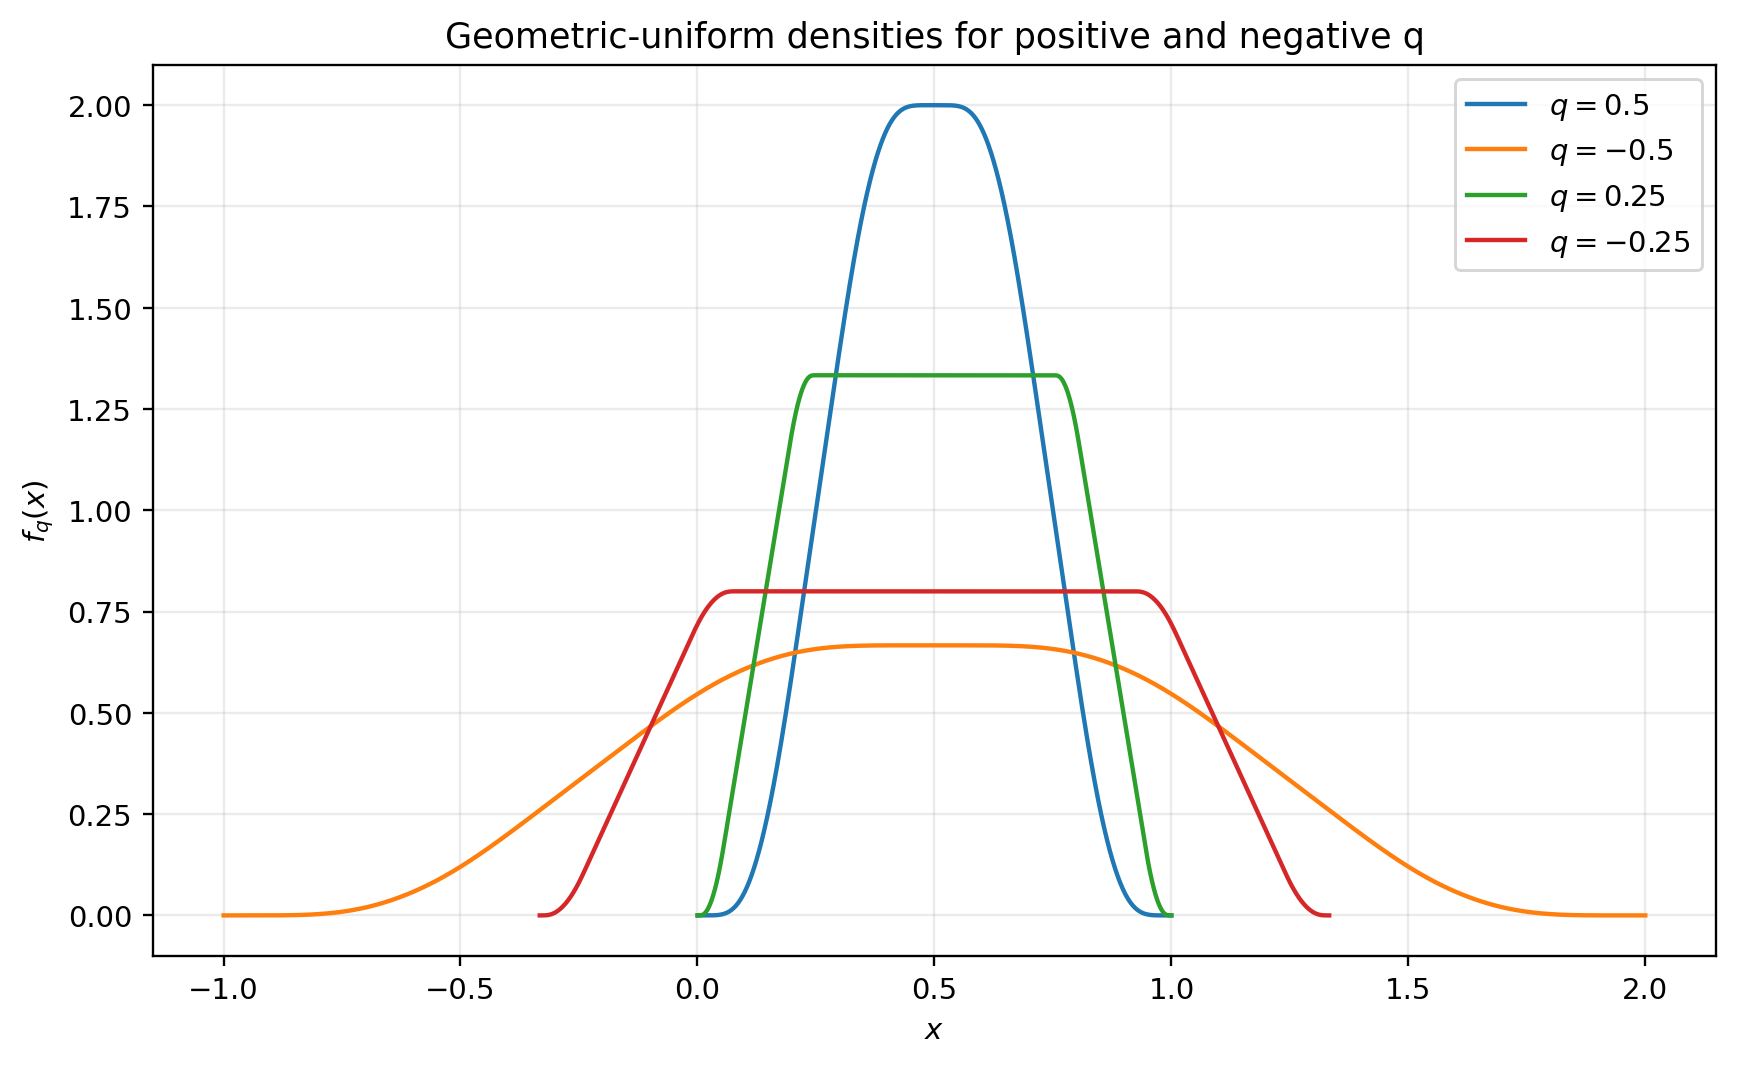
\includegraphics[width=0.9\textwidth]{assets/Fabius_Q_Connections_Report/figures/physical_densities.png}
\caption{Physical densities for $q=\pm\tfrac12,\pm\tfrac14$ (sixteenth-wave
package).  The negative curves are exact affine stretches of their positive
partners; the quarter-base profiles carry positive-length plateaus, while the
half-base plateau is critical and collapses to the center
(\cref{p7:thm:shape}).}
\label{p7:fig:physical-densities}
\end{figure}

Standardizing removes the sign entirely (sixteenth wave): since
$\sigma_{-a}=\lambda_a\sigma_a$, the variance-normalized laws satisfy
$Z_{-a}\overset d=Z_a$, and the support-normalized density profile
\begin{equation}\label{p7:eq:Uq-def}
 \mathcal U_q(x)=R_qg_q\!\left(\tfrac12+R_qx\right),
 \qquad
 R_q=\frac{1-q}{2(1-\abs q)},
 \qquad -1\le x\le1,
\end{equation}
obeys $\mathcal U_{-a}=\mathcal U_a$, with $\mathcal U_{1/2}=\Up$.  All
normalized shape statistics are even functions of $q$.

\subsection{Reciprocal inversion and the Cayley coordinate}

\begin{theorem}[Reciprocal convolution inversion; seventeenth wave]
\label{p7:thm:reciprocity}
For every $q$ off the unit circle,
\begin{equation}\label{p7:eq:reciprocity}
 \boxed{\,M_q(t)\,M_{1/q}(-t)=1,
 \qquad
 C_q(t)\,C_{1/q}(t)=1.\,}
\end{equation}
At the coefficient level, the reciprocal moment row is the signed
binomial-convolution inverse of the original row:
$\sum_{k=0}^n\binom nk m_k(q)(-1)^{n-k}m_{n-k}(1/q)=\delta_{n0}$.
\end{theorem}

\begin{proof}
For $|q|<1$,
$M_{1/q}(-t)^{-1}
=\prod_{j\ge1}E\bigl((1-q^{-1})q^j(-t)\bigr)
=\prod_{j\ge1}E\bigl((1-q)q^{j-1}t\bigr)=M_q(t)$ by
\eqref{p7:eq:Mq-outside}; interchange $q\leftrightarrow1/q$ for the other
case, and combine with reflection for the centered form.
\end{proof}

In the Cayley coordinate $c(q)=(1+q)/(1-q)$ one has $c(-q)=c(q)^{-1}$ and
$c(1/q)=-c(q)$, and the whole calculus is the pair
\begin{equation}\label{p7:eq:cayley-calculus}
 C_{-q}(t)=C_q\bigl(c(q)t\bigr),
 \qquad
 C_{1/q}(t)=C_q(t)^{-1}.
\end{equation}
For the two orbits, with $M=M_{1/2}$ and $N=M_{1/4}$:
\begin{align}
 M_{-1/2}(t)&=\e^{-t}M(3t),
 &M_2(t)&=\e^t/M(t),
 &M_{-2}(t)&=\e^{2t}/M(3t),
 \label{p7:eq:dyadic-orbit}\\
 M_{-1/4}(t)&=\e^{-t/3}N(5t/3),
 &M_4(t)&=\e^t/N(t),
 &M_{-4}(t)&=\e^{4t/3}/N(5t/3).
 \label{p7:eq:quartic-orbit}
\end{align}
Even centered cumulants transform by
$\kappa_{2m}(-q)=c(q)^{2m}\kappa_{2m}(q)$ and
$\kappa_{2m}(1/q)=-\kappa_{2m}(q)$.

\subsection{Finite reciprocal duality by digit reversal}

The germ identity has an exact finite ancestor (sixteenth wave).  For
$q\notin\{0,1\}$ with $q^m\ne1$, the normalized finite law
\begin{equation}\label{p7:eq:finite-law}
 Y_q^{[m]}=\alpha_{m,q}\sum_{j=0}^{m-1}q^jU_j,
 \qquad
 \alpha_{m,q}=\frac{1-q}{1-q^m},
\end{equation}
makes sense for \emph{every} such real $q$, and reversing the iid digit list
proves
\begin{equation}\label{p7:eq:finite-reciprocal}
 \boxed{\,Y_q^{[m]}\overset d=Y_{q^{-1}}^{[m]},\,}
 \qquad\text{and}\qquad
 Y_q^{[m]}\Longrightarrow Y_{q^{-1}}
 \quad(m\to\infty,\ \abs q>1),
\end{equation}
since $\alpha_{m,q}q^{m-1-j}=\alpha_{m,q^{-1}}q^{-j}$.  Thus the exterior
parameters $2,-2,4,-4$, read through normalized finite sums, converge exactly
to the interior laws at $1/2,-1/2,1/4,-1/4$: values $\abs q>1$ must not be
inserted into the infinite series, but they have exact finite and limiting
meanings after normalization and digit reversal.  The germ-level inversion
\eqref{p7:eq:reciprocity} and the finite digit reversal are the analytic and
combinatorial faces of the same duality.
\section{Cumulants, spectral zeta, and shape}
\label{p7:sec:cumulants}

\subsection{The Bernoulli cumulant dictionary}

\begin{theorem}[Signed/reciprocal cumulant dictionary; both waves]
\label{p7:thm:cumulants}
For every $q$ with $q^n\ne1$,
\begin{equation}\label{p7:eq:cumulants}
 \boxed{\ \kappa_1(q)=\frac12,
 \qquad
 \kappa_n(q)=\frac{B_n}{n}\,\frac{(1-q)^n}{1-q^n}
 =\frac{B_n}{n}\,\frac{(1-q)^{n-1}}{[n]_q}
 \quad(n\ge2),\ }
\end{equation}
with $[n]_q=1+q+\cdots+q^{n-1}$; all odd cumulants above the mean vanish, and
\begin{equation}\label{p7:eq:variance}
 \kappa_2(q)=\frac1{12}\,\frac{1-q}{1+q}.
\end{equation}
Moments are complete Bell polynomials,
$m_n(q)=\Bell_n\bigl(\tfrac12,\kappa_2,0,\kappa_4,0,\ldots\bigr)$, hence exact
rationals at every rational $q$.
\end{theorem}

\begin{proof}
Insert $\log E(z)=\tfrac z2+\sum_{n\ge2}\tfrac{B_n}{n}\tfrac{z^n}{n!}$ into
\eqref{p7:eq:Mq-inside} and sum $\sum_{j\ge0}q^{jn}=(1-q^n)^{-1}$; both sides
of \eqref{p7:eq:cumulants} are rational in $q$ order by order and satisfy the
unique recurrence of \cref{p7:thm:formal-unique}, which extends the formula to
the reciprocal regime.
\end{proof}

The M\"obius factor $(1-q)/(1+q)$ already shows the two symmetries at the
level of \eqref{p7:eq:variance}: $\kappa_{2m}(1/q)=-\kappa_{2m}(q)$ (inversion
flips every even centered cumulant) and
$\kappa_{2m}(-q)=c(q)^{2m}\kappa_{2m}(q)$.  The standardized cumulants
\begin{equation}\label{p7:eq:standard-cumulants}
 \kappa_{2m}(Z_q)=\frac{B_{2m}}{2m}\,12^m\,
 \frac{(1-q^2)^m}{1-q^{2m}},
 \qquad
 \kappa_4(Z_q)=-\frac65\,\frac{1-q^2}{1+q^2},
\end{equation}
are even in $q$, making the normalized sign collapse algebraically
transparent.

\begin{statusbox}{Crosswalk to Part VI}
Under the affine identification of \cref{p6:prop:q-crosswalk}
($X_a\overset d=b_a(2Y_q-1)$ at $q=1/a$), the dictionary
\eqref{p7:eq:cumulants} is equivalent to the cumulant formula
\eqref{p6:eq:kappa}, and the standardized kurtosis in
\eqref{p7:eq:standard-cumulants} is the $\lambda_4$ of Part~VI's Gaussian
limit.  Likewise the Lindeberg limit $Z_q\Rightarrow N(0,1)$ as
$\abs q\to1^-$, the uniform limit $Y_q\to U_0$ in $L^2$ as $q\to0$, the
log-Gaussian Fourier envelope, and the exact plateau below are the
$Y_q$-coordinate faces of \cref{p6:sec:parameter-limits},
\cref{p6:eq:Fourier-logGaussian}, and the plateau
\eqref{p6:eq:plateau}; they are stated here once in the $q$ normalization and
not re-proved.
\end{statusbox}

\subsection{Spectral zeta and Fourier decay}

The centered characteristic function is the sinc product
\begin{equation}\label{p7:eq:psi-sinc}
 \psi_q(t)=\E\,\e^{\ii t(Y_q-1/2)}
 =\prod_{n=0}^{\infty}
 \sinc\!\left(\frac{(1-q)q^nt}{2}\right),
 \qquad
 \psi_q(t)=\sinc\!\left(\tfrac{(1-q)t}2\right)\psi_q(qt),
\end{equation}
with positive zeros $\tau_{n,k}=2\pi k/\bigl((1-q)\abs q^n\bigr)$.  The
indexed spectral zeta function evaluates in closed form (sixteenth wave,
specializing the exponent-sequence machinery of Part~I):
\begin{equation}\label{p7:eq:spectral-zeta}
 \Zspec_q(s)=\sum_{n\ge0}\sum_{k\ge1}\tau_{n,k}^{-s}
 =\left(\frac{1-q}{2\pi}\right)^{\!s}\frac{\zeta(s)}{1-\abs q^{\,s}},
 \qquad
 \log\psi_q(t)=-\sum_{m\ge1}\frac{\Zspec_q(2m)}m\,t^{2m},
\end{equation}
and $\kappa_{2m}(q)=(-1)^{m+1}2\,(2m-1)!\,\Zspec_q(2m)$.  The elementary
cutoff argument gives the superpolynomial envelope
$\log\abs{\psi_q(t)}\le-(\log\abs t)^2/(2\lambda)+\bigO_q(\log\abs t)$ with
$\lambda=-\log\abs q$, so for every real $0<\abs q<1$ the law has a compactly
supported $C^\infty$ density, all of whose derivatives vanish at both support
endpoints.  The excluded case $q=0$ (the uniform law) marks a sharp regularity
transition.

\subsection{Log-concavity and the exact plateau phase}

\begin{theorem}[Shape of the whole real family; sixteenth wave]
\label{p7:thm:shape}
For every real $0<\abs q<1$ the density $g_q$ is symmetric about $1/2$,
positive on the interior of its support, log-concave, and unimodal.  For
$0<a\le\tfrac12$,
\begin{equation}\label{p7:eq:plateau}
 g_a(x)=\frac1{1-a}
 \quad\text{on }[a,\,1-a],
 \qquad
 g_{-a}(x)=\frac1{1+a}
 \quad\text{on }\Bigl[\frac{a^2}{1-a},\,1-\frac{a^2}{1-a}\Bigr],
\end{equation}
these being the exact global maxima; for $a<\tfrac12$ the plateaus have
positive length, and at $\abs q=\tfrac12$ they collapse to the central
maximizer.
\end{theorem}

\begin{proof}
Log-concavity: finite partial sums are convolutions of interval uniforms,
which are log-concave by the Pr\'ekopa--Leindler theorem; the class is
weakly closed, and the limit density is smooth.  Plateau: the fixed point \eqref{p7:eq:affine-fixed-point}
writes $g_a$ as the uniform average
$g_a(x)=\tfrac1{1-a}[G_a(x/a)-G_a((x-1+a)/a)]$; for $x\in[a,1-a]$ the first
CDF value is $1$ and the second is $0$.  Convolution with a uniform kernel
gives the matching upper bound, and the negative case is the affine image
under \cref{p7:cor:transport}.
\end{proof}

In Part~VI coordinates the positive plateau is exactly the central plateau of
$h_a$ at $a=1/q$; the phase boundary $\abs q=\tfrac12$ is the critical base
$a=2$.  The conjecture that $\mathcal U_q$ is \emph{strictly} log-concave for
$\tfrac12<\abs q<1$ is the register entry already recorded in Part~VI's
future directions and is not repeated here.

\section{Scale multisection and the half--quarter bridge}
\label{p7:sec:multisection}

\begin{theorem}[Geometric multisection; both waves]
\label{p7:thm:multisection}
Let $m\ge2$ and $[m]_q\ne0$, $q^n\ne1$.  As analytic germs,
\begin{equation}\label{p7:eq:M-multisection}
 \boxed{\ M_q(t)=\prod_{r=0}^{m-1}
 M_{q^m}\!\left(\frac{q^r}{[m]_q}\,t\right),\ }
\end{equation}
and for $\abs q<1$ this is the distributional identity
\begin{equation}\label{p7:eq:Y-multisection}
 Y_q\overset d=\sum_{r=0}^{m-1}\frac{q^r}{[m]_q}\,Y_{q^m}^{(r)}
\end{equation}
with independent summands.  The cumulant compatibility check is the
$q$-integer identity
$\sum_{r<m}\bigl(q^r/[m]_q\bigr)^n=[m]_{q^n}/[m]_q^n$.
\end{theorem}

\begin{proof}
Split the digit index as $j=mk+r$; the inner sums are independent copies of
$Y_{q^m}$ with weights $(1-q)q^r/(1-q^m)$.  The reciprocal regime follows from
the product definition \eqref{p7:eq:Mq-outside} by the same reindexing.
\end{proof}

The specializations at $m=2$ organize the two orbits into one system:
\begin{align}
 Y_{1/2}&\overset d=\tfrac23Y_{1/4}^{(0)}+\tfrac13Y_{1/4}^{(1)},
 \label{p7:eq:half-quarter}\\
 Y_{-1/2}&\overset d=2Y_{1/4}^{(0)}-Y_{1/4}^{(1)},
 \qquad
 M_2(t)=M_4(t/3)\,M_4(2t/3),
 \label{p7:eq:signed-reciprocal-decimation}
\end{align}
and more generally
$Y_{1/2}\overset d=(2^m-1)^{-1}\sum_{j<m}2^{m-1-j}Y_{2^{-m}}^{(j)}$: the
Fabius law is a convolutional barycenter of the $q=2^{-m}$ family.  In the
unnormalized centered coordinate $R_q=\sum_{j\ge0}q^jV_j$ the identity is
cleaner still (seventeenth wave),
\begin{equation}\label{p7:eq:R-multisection}
 R_q\overset d=\sum_{r=0}^{m-1}q^rR_{q^m}^{(r)},
 \qquad\text{so at }q=\tfrac12,\ m=2:\qquad
 u_{1/2}=u_{1/4}*\bigl(2u_{1/4}(2\,\cdot)\bigr),
\end{equation}
where $u_q$ denotes the density of $R_q$ ($u_{1/2}$ is the Rvachev bump in
its standard support normalization); the sixteenth wave states the same fact
as $\Up=\mathcal D_{2/3}\,\mathcal U_{1/4}*\mathcal D_{1/3}\,\mathcal U_{1/4}$
with $\mathcal D_c$ the $L^1$-dilation by $c$.  Multisection is
simultaneously: an independent-sum decomposition of random digits, a
convolution of densities, a factorization of Fourier products, and the
elementary Pochhammer dissection
$(a;q)_\infty=\prod_{r<m}(aq^r;q^m)_\infty$ --- the same identity in four
coordinate systems, not four analogies.

\section{Spectral \texorpdfstring{$q^2$}{q\^2}-Pochhammer products and zero divisors}
\label{p7:sec:spectral}

\subsection{The factorization inside and outside the disk}

\begin{theorem}[Spectral Pochhammer factorization; both waves]
\label{p7:thm:sinc-poch}
For real $\abs q<1$,
\begin{equation}\label{p7:eq:sinc-poch}
 \boxed{\ \psi_q(t)=\prod_{k=1}^{\infty}
 \left(\frac{(1-q)^2t^2}{4\pi^2k^2};\,q^2\right)_{\!\infty},\ }
\end{equation}
locally uniformly in $t\in\C$; equivalently
$M_q(t)=\e^{t/2}\prod_k\bigl(-\tfrac{(1-q)^2t^2}{4\pi^2k^2};q^2\bigr)_\infty$.
For $\abs q>1$ (seventeenth wave),
\begin{equation}\label{p7:eq:sinc-poch-outside}
 M_q(t)=\e^{t/2}\prod_{k=1}^{\infty}
 \left(-\frac{(1-q^{-1})^2t^2}{4\pi^2k^2};\,q^{-2}\right)_{\!\infty}^{-1}:
\end{equation}
inversion is literally a zero--pole exchange in the same contracting nome.
\end{theorem}

\begin{proof}
Insert Euler's product $\sinc z=\prod_k(1-z^2/\pi^2k^2)$ into every factor of
\eqref{p7:eq:psi-sinc}; absolute convergence of the double perturbation series
permits reordering, and the product over the scale index is a
$q^2$-Pochhammer symbol.  Outside the disk, apply this to $1/C_{1/q}$.
\end{proof}

The nome is $q^2$, not $q$: centering makes every factor even, and evenness
forgets the sign of each geometric scale.  Thus $q=\pm\tfrac12$ share nome
$\tfrac14$ and $q=\pm\tfrac14$ share nome $\tfrac1{16}$, with
$\psi_{-1/2}(t)=\psi_{1/2}(3t)$ and $\psi_{-1/4}(t)=\psi_{1/4}(5t/3)$, while
their reciprocals use the same nomes with inverse factors.  Multisection of
the random digits and multisection of the Pochhammer product are the same
identity (sixteenth wave): dissecting \eqref{p7:eq:sinc-poch} by
$(a;Q)_\infty=\prod_{j<m}(aQ^j;Q^m)_\infty$ reproduces
\cref{p7:thm:multisection} factor by factor.

\subsection{Integer zero divisors at reciprocal-integer ratio}

For the base-$b$ member it is convenient to renormalize the centered
transform as
\begin{equation}\label{p7:eq:Phi-q}
 \Phi_q(z)=\prod_{j=0}^{\infty}\sinc(\pi q^jz)
 \qquad(\abs q<1),
\end{equation}
so that at $q=1/b$ the factor $j=0$ vanishes exactly at the nonzero integers.

\begin{proposition}[Base-$b$ zero divisor; seventeenth wave]
\label{p7:prop:base-b-zero}
Let $q=1/b$ with integer $b\ge2$.  At every nonzero integer $n$,
\begin{equation}\label{p7:eq:base-b-zero}
 \ord_{z=n}\Phi_{1/b}(z)=1+\nu_b(n),
 \qquad
 \nu_b(n)=\max\{j\ge0:b^j\mid n\}.
\end{equation}
In particular $\ord_{z=n}\Phi_{1/4}(z)=1+\floor{\vtwo(n)/2}$: the quartic
transform sees binary valuation levels in pairs, the spectral counterpart of
even/odd scale decimation.
\end{proposition}

\begin{proof}
The factor $\sinc(\pi z/b^j)$ vanishes simply at $z=n\ne0$ exactly when
$b^j\mid n$, that is, for $0\le j\le\nu_b(n)$; all other factors are nonzero
there.
\end{proof}

At $b=2$ this is the classical multiplicity $1+\vtwo(n)$ of the dyadic
corpus; the general-$b$ statement is the single-scale case of Part~I's
exponent-sequence zero calculus.
\section{Reciprocal Laplace duality and vertical moment geometry}
\label{p7:sec:laplace-dual}

The formal variance $-\kappa_2(1/q)$ of a reciprocal germ is negative, so
$M_q$ with $q>1$ is the MGF of no real probability law.  The seventeenth wave
resolves this positively: the obstruction disappears on a vertical line.

\begin{theorem}[Positive Laplace representation; seventeenth wave]
\label{p7:thm:laplace-dual}
Let $\abs q>1$, $r=1/q$, and let $Z_{j,k}$ ($j\ge0$, $k\ge1$) be independent
standard symmetric Laplace variables (density $\tfrac12\e^{-\abs x}$).  With
scales $b_{j,k}(r)=\abs{1-r}\,\abs r^j/(2\pi k)$, the double series
\begin{equation}\label{p7:eq:Lr}
 L_{r}=\sum_{j\ge0}\sum_{k\ge1}b_{j,k}(r)\,Z_{j,k}
\end{equation}
converges almost surely and in $L^2$, and
\begin{equation}\label{p7:eq:C-laplace}
 \boxed{\ C_q(t)=\E\,\e^{\ii tL_{r}},
 \qquad
 m_n(q)=\E\Bigl(\tfrac12+\ii L_{r}\Bigr)^{n}.\ }
\end{equation}
The reciprocal moments are ordinary polynomial moments of a positive measure
on the vertical line $\Re z=\tfrac12$.
\end{theorem}

\begin{proof}
By \eqref{p7:eq:sinc-poch} and reciprocity,
$C_q(t)=1/C_r(t)=\prod_{j,k}\bigl(1+b_{j,k}(r)^2t^2\bigr)^{-1}$, the
characteristic function of the displayed Laplace convolution;
$\sum b_{j,k}^2=(1-r)^2\zeta(2)/(4\pi^2(1-r^2))<\infty$ gives Kolmogorov
convergence, and $M_q(t)=\e^{t/2}C_q(t)=\E\exp\bigl(t(\tfrac12+\ii
L_r)\bigr)$ near $0$.
\end{proof}

The Laplace cumulants close the circle through Euler's evaluation: a Laplace
variable of scale $b$ has even cumulants $(2m)!\,b^{2m}/m$, so
$\kappa_{2m}(L_r)$ is a $\zeta(2m)$-sum over the double lattice, and
$B_{2m}=(-1)^{m+1}2(2m)!\zeta(2m)/(2\pi)^{2m}$ turns it into
$\kappa_{2m}(q)=(-1)^m\kappa_{2m}(L_r)$ --- exactly the $\ii^{2m}$ of the
vertical embedding.

\begin{theorem}[Hankel signature; seventeenth wave]
\label{p7:thm:hankel}
For real $\abs q>1$ and every $n\ge1$, the moment Hankel determinant
$\Delta_n(q)=\det(m_{i+j}(q))_{0\le i,j<n}$ satisfies
\begin{equation}\label{p7:eq:hankel-signature}
 \boxed{\ \sgn\Delta_n(q)=(-1)^{\binom n2},\ }
\end{equation}
and no $\Delta_n(q)$ vanishes.
\end{theorem}

\begin{proof}
The real Hankel determinant $H_n$ of $L_r$ is strictly positive (its law has
full support, so $1,x,\ldots,x^{n-1}$ are independent in $L^2$).  Translating
a moment sequence is a unit-triangular change of basis, and scaling by $a$
multiplies the $n$th determinant by $a^{n(n-1)}$; applying both to
$\tfrac12+\ii L_r$ gives $\Delta_n(q)=\ii^{\,n(n-1)}H_n=(-1)^{\binom n2}H_n$.
\end{proof}

Consequently the reciprocal moment functional is quasi-definite: its monic
orthogonal polynomials exist, satisfy
$P_{n+1}(z)=(z-\tfrac12)P_n(z)+\beta_n^{(r)}P_{n-1}(z)$ with
$\beta_n^{(r)}>0$ inherited from the symmetric Jacobi recurrence of $L_r$, and
have all zeros on $\Re z=\tfrac12$.  Reciprocal $q$ does not destroy
positivity; it rotates it onto a vertical line.  Determining the Jacobi
coefficients $\beta_n^{(r)}$, their asymptotics, and their relation to the
double geometric/harmonic scale lattice is posed in the frontier section.

\section{\texorpdfstring{$q$}{q}-Fabius--Bernoulli Appell polynomials}
\label{p7:sec:appell}

On polynomials, geometric averaging $(\mathcal A_rf)(x)=\E f(x+Y_r)$ is the
multiplier $M_r(D)$, so reciprocity identifies its inverse with no triangular
solve (seventeenth wave):
\begin{equation}\label{p7:eq:averaging-inverse}
 \boxed{\ \mathcal A_r^{-1}=M_{1/r}(-D).\ }
\end{equation}
The reciprocal germ is the deconvolution symbol for geometric-uniform
smoothing.  Define the Appell family
\begin{equation}\label{p7:eq:appell-gen}
 \sum_{n\ge0}\Br_n^{(r)}(x)\frac{t^n}{n!}
 =\frac{\e^{xt}}{M_r(t)},
\end{equation}
so that $\tfrac{\dd}{\dd x}\Br_n^{(r)}=n\Br_{n-1}^{(r)}$ and
\begin{equation}\label{p7:eq:appell-deconvolution}
 \boxed{\ \E\,\Br_n^{(r)}(x+Y_r)=x^n.\ }
\end{equation}
The family interpolates two classical boundaries:
\begin{equation}\label{p7:eq:appell-boundaries}
 \Br_n^{(0)}(x)=B_n(x)
 \quad\text{(ordinary Bernoulli polynomials)},
 \qquad
 \Br_n^{(r)}(x)\longrightarrow\Bigl(x-\tfrac12\Bigr)^{n}
 \quad(r\to1^-),
\end{equation}
and from outside the disk,
$M_q(t)\to t\e^t/(\e^t-1)=\sum B_n(1)t^n/n!$ as $\abs q\to\infty$: Bernoulli
polynomials sit at both ends of the sign/reciprocal diagram.  The Mahler
equation induces the refinement
\begin{equation}\label{p7:eq:appell-mahler}
 \Br_n^{(r)}(x)=
 \sum_{k=0}^{n}\binom nk B_k\,(1-r)^kr^{\,n-k}\,
 \Br_{n-k}^{(r)}\!\left(\frac xr\right)
\end{equation}
(with $B_1=-\tfrac12$), a Bernoulli-polynomial analogue of the Fabius Mahler
equation; and the Bell form
$\Br_n^{(r)}(x)=\Bell_n\bigl(x-\tfrac12,-\kappa_2(r),0,-\kappa_4(r),0,
\ldots\bigr)$ gives
\[
 \Br_2^{(r)}=z^2-v_r,\quad
 \Br_3^{(r)}=z^3-3v_rz,\quad
 \Br_4^{(r)}=z^4-6v_rz^2+3v_r^2-\kappa_4(r),
 \qquad z=x-\tfrac12,\ v_r=\kappa_2(r),
\]
with the reflection $\Br_n^{(r)}(1-x)=(-1)^n\Br_n^{(r)}(x)$.  Their
arithmetic (von Staudt--Clausen analogues, multiplication theorems, root
geometry) is a fresh research program.

\section{The Fabius--Pochhammer moment polynomial}
\label{p7:sec:moment-polynomial}

The exponential moments $a_n(q)$ have poles at roots of unity.  Clearing them
with the finite Pochhammer symbol produces a polynomial invariant
(seventeenth wave):
\begin{equation}\label{p7:eq:Pn-def}
 \boxed{\ \mathcal P_n(q)=\frac{(q;q)_n}{(1-q)^n}\,\frac{m_n(q)}{n!}.\ }
\end{equation}

\begin{theorem}[Polynomial recurrence and boundaries]
\label{p7:thm:Pn}
$\mathcal P_n\in\Q[q]$ with $\deg\mathcal P_n\le\binom n2$,
$\mathcal P_0=1$, and
\begin{equation}\label{p7:eq:Pn-recurrence}
 \mathcal P_n(q)=
 \sum_{k=0}^{n-1}\frac{q^k}{(n-k+1)!}\,
 \frac{(q;q)_{n-1}}{(q;q)_k}\,\mathcal P_k(q),
\end{equation}
with boundary data
$\mathcal P_n(0)=\tfrac1{(n+1)!}$ and leading coefficient
$[q^{\binom n2}]\mathcal P_n=B_n(1)/n!$ (so odd $n>1$ drop strictly below the
degree bound).
\end{theorem}

\begin{proof}
Multiply \eqref{p7:eq:an-recurrence} by $(q;q)_{n-1}/(1-q)^n$ and substitute
$a_k=(1-q)^k\mathcal P_k/(q;q)_k$; the quotient
$(q;q)_{n-1}/(q;q)_k$ is a polynomial and the degree bound follows by
induction.  At $q=0$ only $k=0$ survives; as $q\to\infty$,
$m_n(q)/n!\to B_n(1)/n!$ while $(q;q)_n/(1-q)^n\sim q^{\binom n2}$.
\end{proof}

The first values are
\[
 \mathcal P_1=\tfrac12,\qquad
 \mathcal P_2=\frac{q+2}{12},\qquad
 \mathcal P_3=\frac{q^2+q+1}{24},
\]
\[
 \mathcal P_4=-\frac{(q^2+q+1)(q^4-2q^3-5q^2-3q-6)}{720},
\]
and the exact factorizations continue with
\begin{align}
 \mathcal P_5&=-\frac{[3]_q[5]_q\,(q^3-2q^2-2)}{1440},
 \notag\\
 \mathcal P_7&=\frac{[3]_q[5]_q[7]_q\,
 (2q^8-6q^7+4q^6-3q^5+6q^4-4q^3+7q^2+3)}{120960},
 \label{p7:eq:Pn-factorizations}
\end{align}
with an analogous $[3]_q[5]_q$ factor in $\mathcal P_6$.

\begin{conjecture}[Odd $q$-integer divisor; seventeenth wave]
\label{p7:conj:Pn-divisibility}
For every $n\ge3$,
$\prod_{3\le d\le n,\ d\ \mathrm{odd}}[d]_q$ divides $\mathcal P_n(q)$ in
$\Q[q]$.  Checked symbolically through $n=16$.  Since
$\prod_{d}[d]_q=\prod_e\Phi_e(q)^{\floor{(\floor{n/e}+1)/2}}$ over odd
cyclotomic indices $e$, repeated cyclotomic jets --- not mere vanishing at
primitive odd roots of unity --- must be controlled; the cancellation-order
calculus of the two-nome partition function below is a candidate mechanism.
\end{conjecture}

The polynomial is not decorative: the exact endpoint lattice of
\cref{p7:sec:endpoints} reads
$G_q(q^n)=q^{\binom{n+1}2}\mathcal P_n(q)/(q;q)_n$, so $(q;q)_n$ is precisely
the pole-clearing factor of the moment recurrence surfacing as the endpoint
denominator --- Mersenne factors at $q=\tfrac12$, factors $4^j-1$ at
$q=\tfrac14$.
\section{Two master products on the binary cube}
\label{p7:sec:master-products}

The Thue--Morse product and the $q$-Pochhammer symbol are unified twice over
by the two waves, through two complementary four-parameter products.  For
$\epsilon\in\{0,1\}^N$ write
$\abs\epsilon=\sum_j\epsilon_j$ (Hamming weight),
$\Omega(\epsilon)=\sum_jj\epsilon_j$ (position energy), and
$A_{\sigma,N}(\epsilon)=\sum_j\epsilon_j\sigma^j$ (geometric projection).

\subsection{The two-nome partition function}

\begin{definition}[Seventeenth wave]
\label{p7:def:two-nome}
For parameters $u,t,\rho,\sigma$ set
\begin{equation}\label{p7:eq:Z-master}
 \Zpart_N(u,t;\rho,\sigma)=
 \prod_{j=0}^{N-1}\bigl(1-u\rho^j\e^{t\sigma^j}\bigr)
 =\sum_{\epsilon\in\{0,1\}^N}
 (-u)^{\abs\epsilon}\rho^{\Omega(\epsilon)}
 \e^{tA_{\sigma,N}(\epsilon)}.
\end{equation}
\end{definition}

Its $t=0$ face is finite Pochhammer/Gaussian calculus,
$\Zpart_N(u,0;\rho,\sigma)=(u;\rho)_N
=\sum_k(-u)^k\rho^{\binom k2}\qbinom Nk\rho$; its $(u,\rho)=(1,1)$ face is
the geometric Prouhet generator
$\prod_{j<N}(1-\e^{t\sigma^j})$.  The $q$-Pochhammer and Thue--Morse products
are perpendicular faces of one object, and the two nomes must not be
identified prematurely.  Splitting $j=mk+r$ gives simultaneous multisection in
both nomes,
\begin{equation}\label{p7:eq:Z-multisection}
 \Zpart_{mN}(u,t;\rho,\sigma)
 =\prod_{r=0}^{m-1}
 \Zpart_N\bigl(u\rho^r,\,t\sigma^r;\,\rho^m,\sigma^m\bigr),
\end{equation}
whose faces are finite Pochhammer dissection and the comb convolution law of
\cref{p7:sec:comb}, and whose normalized Prouhet jet recovers
\cref{p7:thm:multisection}.  The mixed coefficients
$\mathcal M_{N,k,m}=\sum_{\abs\epsilon=k}\rho^{\Omega(\epsilon)}
A_{\sigma,N}(\epsilon)^m=(-1)^km!\,[u^kt^m]\Zpart_N$ refine each Gaussian row
by geometric power moments, and the order of vanishing at $t=0$ is exactly
$\#\{j<N:u\rho^j=1\}$ --- classical Prouhet cancellation is the maximal case
$u=\rho=1$, while root-of-unity nomes select arithmetic progressions of digit
positions and give exactly controlled \emph{partial} Prouhet cancellations.

\subsection{The digit-position product and its position-parity companion}

The sixteenth wave couples the position energy to the \emph{encoded integer}
instead of the projected moment.  With $b_j(n)$ the binary digits of
$n<2^m$, $\wt(n)=\sum_jb_j(n)$, and $\pi_2(n)=\sum_jj\,b_j(n)$,
\begin{equation}\label{p7:eq:digit-master}
 \Xi_m(u,z;q)=\prod_{j=0}^{m-1}\bigl(1-uq^jz^{2^j}\bigr)
 =\sum_{n=0}^{2^m-1}(-u)^{\wt(n)}q^{\pi_2(n)}z^n,
\end{equation}
which simultaneously tracks the integer, its Hamming weight, and its occupied
bit positions.  Setting $z=1$ gives
$(u;q)_m=\sum_{n<2^m}(-u)^{\wt(n)}q^{\pi_2(n)}$, and at fixed weight
\begin{equation}\label{p7:eq:fixed-weight}
 \sum_{\substack{n<2^m\\ \wt(n)=k}}q^{\pi_2(n)}
 =q^{\binom k2}\qbinom mkq,
\end{equation}
a specialization of the $q$-digital binomial theorem of Mansour and
Nguyen~\cite{p7:mansour-nguyen}.  The shifted variant
$\mathcal T_m(z;q)=\prod_{j<m}(1-q^{j+1}z^{2^j})
=\sum_n(-1)^{\wt(n)}q^{\rho_2(n)}z^n$ with
$\rho_2=\pi_2+\wt$ satisfies
$\mathcal T_m(1;q)=(q;q)_m$; at negative nome $q=-r$ its coefficients become
$\chi(n)r^{\rho_2(n)}$ with the \emph{position parity}
$\chi(n)=(-1)^{\pi_2(n)}$.  The pair
$\bigl((-1)^{\wt(n)},\chi(n)\bigr)$ is $2$-automatic with the four-state
recurrences
\begin{equation}\label{p7:eq:four-state}
 \chi(2n)=\chi(2n+1)=\chi(n)\,(-1)^{\wt(n)},
\end{equation}
since doubling shifts every occupied position by one.  The infinite product
satisfies the Mahler equation
$\Xi_\infty(u,z;q)=(1-uz)\,\Xi_\infty(uq,z^2;q)$ and the finite reciprocity
$\Xi_m(u,z;q)=(-u)^mq^{\binom m2}z^{2^m-1}\Xi_m(u^{-1},z^{-1};q^{-1})$ ---
the digit-polynomial counterpart of the reciprocal law and the Lagrange row
reversal below.

\subsection{Prouhet moment transfer, desingularization, and Bell--Bernoulli}

The Prouhet face carries an exact moment calculus, stated by the two waves in
two equivalent dresses and merged here.

\begin{theorem}[$q$-Prouhet moment transfer; both waves]
\label{p7:thm:q-prouhet}
Let $q\ne0$ be complex, $N\ge1$, and let
$S_{N,m}(q)=\sum_{\epsilon}(-1)^{\abs\epsilon}A_{q,N}(\epsilon)^m$ be the
signed power sums of the geometric subset sums.  With
$T_{q,N}=\sum_{j<N}q^jU_j$,
\begin{equation}\label{p7:eq:q-prouhet}
 S_{N,m}(q)=0\quad(0\le m<N),
 \qquad
 \boxed{\ S_{N,N+\ell}(q)
 =(-1)^N\frac{(N+\ell)!}{\ell!}\,q^{\binom N2}\,
 \E\,T_{q,N}^{\,\ell}\ }
 \quad(\ell\ge0).
\end{equation}
Equivalently (general-radix Bell--Bernoulli form), the same subset sums obey
\begin{gather}
 S_{N,N+\ell}(q)
 =(-1)^Nq^{\binom N2}\frac{(N+\ell)!}{\ell!}\,
 \Bell_\ell\bigl(\gamma_1,\ldots,\gamma_\ell\bigr),
 \label{p7:eq:radix-bell}\\
 \gamma_1=\tfrac12[N]_q,\qquad
 \gamma_{2r}=\frac{B_{2r}}{2r}\,[N]_{q^{2r}},\qquad
 \gamma_{2r+1}=0\quad(r\ge1),\notag
\end{gather}
and the finite product desingularizes into a normalized moment transform:
with $\alpha_{N,q}=(1-q)/(1-q^N)$,
\begin{equation}\label{p7:eq:desingularization}
 \E\,\e^{t\left(Y_q^{[N]}-1/2\right)}
 =\frac{(-1)^N\e^{-t/2}\,
 \prod_{j<N}\bigl(1-\e^{\alpha_{N,q}q^jt}\bigr)}
 {\alpha_{N,q}^{\,N}\,q^{\binom N2}\,t^{\,N}},
\end{equation}
which for $\abs q>1$ converges locally uniformly to the centered transform of
$Y_{1/q}$.
\end{theorem}

\begin{proof}
Factor $1-\e^{z}=-zE(z)$ in each term of the Prouhet face:
$\prod_{j<N}(1-\e^{q^jt})=(-1)^Nq^{\binom N2}t^N\prod_{j<N}E(q^jt)$.  The
explicit $t^N$ proves the vanishings; comparing the coefficient of
$t^{N+\ell}$ gives \eqref{p7:eq:q-prouhet}, and expanding
$\log\prod E(q^jt)$ by the uniform cumulant series gives
\eqref{p7:eq:radix-bell} (the two right sides are the same number:
$\E T_{q,N}^{\ell}=\ell!\,[t^\ell]\prod_{j<N}E(q^jt)$).  Dividing by the
maximal Prouhet zero and centering gives \eqref{p7:eq:desingularization},
and \eqref{p7:eq:finite-reciprocal} identifies the $\abs q>1$ limit.
\end{proof}

The first surviving moment is $S_{N,N}(q)=(-1)^NN!\,q^{\binom N2}$, and every
$q$-Fabius moment is a normalized limit of first nonvanishing Thue--Morse
jets:
$m_\ell(q)=(1-q)^\ell\lim_N(-1)^Nq^{-\binom N2}
\tfrac{\ell!}{(N+\ell)!}S_{N,N+\ell}(q)$.  In particular
$b=2,-2,4,-4$ produce, through renormalized classical, negabinary, base-four,
and negative base-four Thue--Morse exponential sums, exactly the laws at
$q=\tfrac12,-\tfrac12,\tfrac14,-\tfrac14$.  The Fabius MGF is the normalized
residual jet of the maximal Prouhet zero
(\cref{p7:eq:desingularization} at $N\to\infty$; the same statement in the
partition-function coordinate is
$M_q(t)=\lim_N\Zpart_N(1,(1-q)t;1,q)\cdot
\bigl[(-1)^N(1-q)^Nq^{\binom N2}t^N\bigr]^{-1}$).

Two parity remarks connect the layers (sixteenth wave).  Centering the finite
transform turns each factor into a hyperbolic sine; since $\sinh$ is odd, the
radix sign change accumulates a global parity,
\begin{equation}\label{p7:eq:sinh-parity}
 \e^{-\frac12[N]_{-a}t}\,\prod_{j<N}\bigl(1-\e^{(-a)^jt}\bigr)
 =(-1)^{\binom N2}\,
 \e^{-\frac12[N]_{a}t}\,\prod_{j<N}\bigl(1-\e^{a^jt}\bigr),
\end{equation}
whereas the continuous centered factors are even sincs and absorb signs
invisibly.  At the measure level (seventeenth wave), the signed comb
$\Delta_{q,N}=\sum_\epsilon(-1)^{\abs\epsilon}\delta_{A_{q,N}(\epsilon)}$
transports by
\begin{equation}\label{p7:eq:comb-transport}
 \Delta_{-a,N}=(-1)^{\floor{N/2}}\,\tau_{-c_{a,N}}\,\Delta_{a,N},
 \qquad
 \Delta_{q^{-1},N}=(D_{q^{-(N-1)}})_*\,\Delta_{q,N},
\end{equation}
($\tau_c$ translation, $D_c$ dilation, $c_{a,N}=a(1-a^{2\floor{N/2}})/(1-a^2)$,
by complementing odd-position digits and by digit reversal respectively):
sign is translation up to a global parity, inversion is dilation.  The
Klein-four geometry acts identically on the infinite germ and on every finite
comb.

\section{Position-energy layers and the finite-geometry square}
\label{p7:sec:position-energy}

At fixed Hamming weight the position-energy layer is Gaussian,
$H_{N,k}(\rho)=\sum_{\abs\epsilon=k}\rho^{\Omega(\epsilon)}
=\rho^{\binom k2}\qbinom Nk\rho$, with reciprocity
$H_{N,k}(\rho)=\rho^{k(N-1)}H_{N,k}(\rho^{-1})$ and
$\qbinom Nk\rho=\rho^{k(N-k)}\qbinom Nk{\rho^{-1}}$.  At negative nome the
signs are governed by two quadratic parities (seventeenth wave):
\begin{equation}\label{p7:eq:H-signs}
 \sgn H_{N,k}(-a)=(-1)^{\binom k2}
 \quad(0<a<1),
 \qquad
 \sgn H_{N,k}(-a)=(-1)^{\binom k2+k(N-k)}
 \quad(a>1),
\end{equation}
and pairing factors splits the negative row into two positive $a^2$-rows,
$(z;-a)_{2m}=(z;a^2)_m(-az;a^2)_m$ --- the finite counterpart of sign
conjugacy and decimation.  Interpreting the nome as a prime power connects
the two orbits to finite geometry: $\qbinom NkQ$ counts $k$-planes in
$\mathbb F_Q^N$, $\qbinom Nk{1/Q}=Q^{-k(N-k)}\#\Gr(k,\mathbb F_Q^N)$, and by
Fu, Reiner, Stanton, and Thiem~\cite{p7:fu-reiner-stanton-thiem} the negative
nome counts nondegenerate subspaces of Hermitian spaces:
$\qbinom Nk{-Q}=(-Q)^{-k(N-k)}U_Q(N,k)$ and
$\qbinom Nk{-1/Q}=Q^{-2k(N-k)}U_Q(N,k)$ over $\mathbb F_{Q^2}$.  The two
orbits therefore carry a finite-geometry square: $\pm2,\pm\tfrac12$
correspond to Grassmannians over $\mathbb F_2$ and Hermitian geometry over
$\mathbb F_4$; $\pm4,\pm\tfrac14$ to $\mathbb F_4$ and $\mathbb F_{16}$.
(For example $\#\Gr(2,\mathbb F_2^4)=35$ and $U_2(4,2)=240$ give
$\qbinom42{1/2}=35/16$ and $\qbinom42{-1/2}=15/16$.)

\section{Box-spline combs and the quartic Cantor skeleton}
\label{p7:sec:comb}

The centered finite law $R_{q,N}=\sum_{j<N}q^jV_j$ is a nonuniform box
spline: with radius $A^{\mathrm{rad}}_{q,N}=\tfrac12\sum_{j<N}q^j$,
\begin{gather}
 B_{q,N}(x)=\frac1{(N-1)!\,q^{\binom N2}}
 \sum_{\epsilon\in\{0,1\}^N}(-1)^{\abs\epsilon}
 \pospart{x+A^{\mathrm{rad}}_{q,N}-A_{q,N}(\epsilon)}^{\,N-1},
 \label{p7:eq:box-spline}\\
 D^NB_{q,N}=q^{-\binom N2}\,
 \tau_{-A^{\mathrm{rad}}_{q,N}}\,\Delta_{q,N},\notag
\end{gather}
so the $q$-Prouhet cancellation is precisely the vanishing of the first $N-1$
distributional moments of the derivative comb, and $N$-fold integration
converts the signed atoms into a positive spline.  At $q=\tfrac12$ the knots
$A_{1/2,N}(\epsilon)$ fill a complete dyadic grid and the signs are the
Thue--Morse sequence in binary order; at $q=\tfrac14$ the knots use only the
digits $\{0,1\}$ in base four, and their infinite closure is the self-similar
set
\begin{equation}\label{p7:eq:quartic-cantor}
 K^{\mathrm{raw}}_4=\Bigl\{\sum_{j\ge0}\epsilon_j4^{-j}:
 \epsilon_j\in\{0,1\}\Bigr\},
 \qquad
 \dim_{\mathrm H}K^{\mathrm{raw}}_4=\frac{\log2}{\log4}=\frac12.
\end{equation}
The finite derivative comb is a signed Cantor skeleton even though the
limiting density is $C^\infty$ with full interval support: integration
through arbitrarily many uniform scales erases the gaps.  The comb
multisection
\begin{equation}\label{p7:eq:comb-multisection}
 \Delta_{q,2N}=\Delta_{q^2,N}*(D_q)_*\Delta_{q^2,N}
\end{equation}
factors the full dyadic Thue--Morse comb into a convolution of two quartic
Cantor combs --- the singular, derivative-level ancestor of the smooth
convolution \eqref{p7:eq:half-quarter}.  (This comb calculus complements the
dyadic-comb quadrature volume of the corpus, which studies unsigned
equal-weight combs against $F$; here the combs are the signed Thue--Morse
derivative skeletons of the family itself.)

\begin{figure}[H]
\centering
\begin{minipage}[t]{0.48\textwidth}
\centering
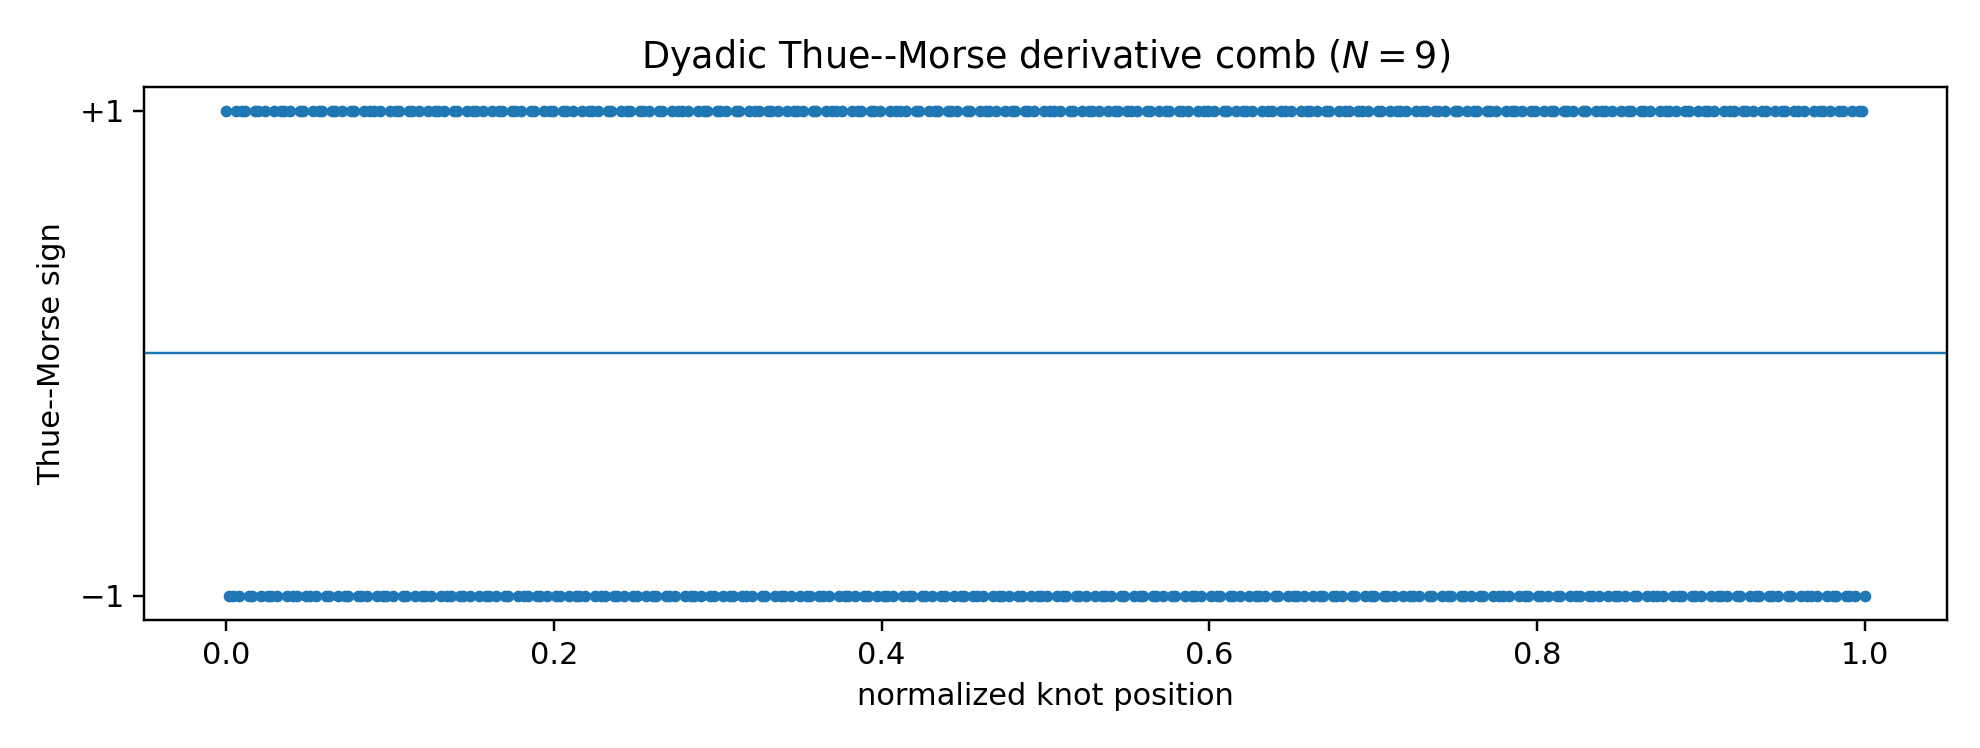
\includegraphics[width=\textwidth]{assets/Signed_Reciprocal_q_Fabius_Frontiers/dyadic_thue_morse_comb.png}
\end{minipage}\hfill
\begin{minipage}[t]{0.48\textwidth}
\centering
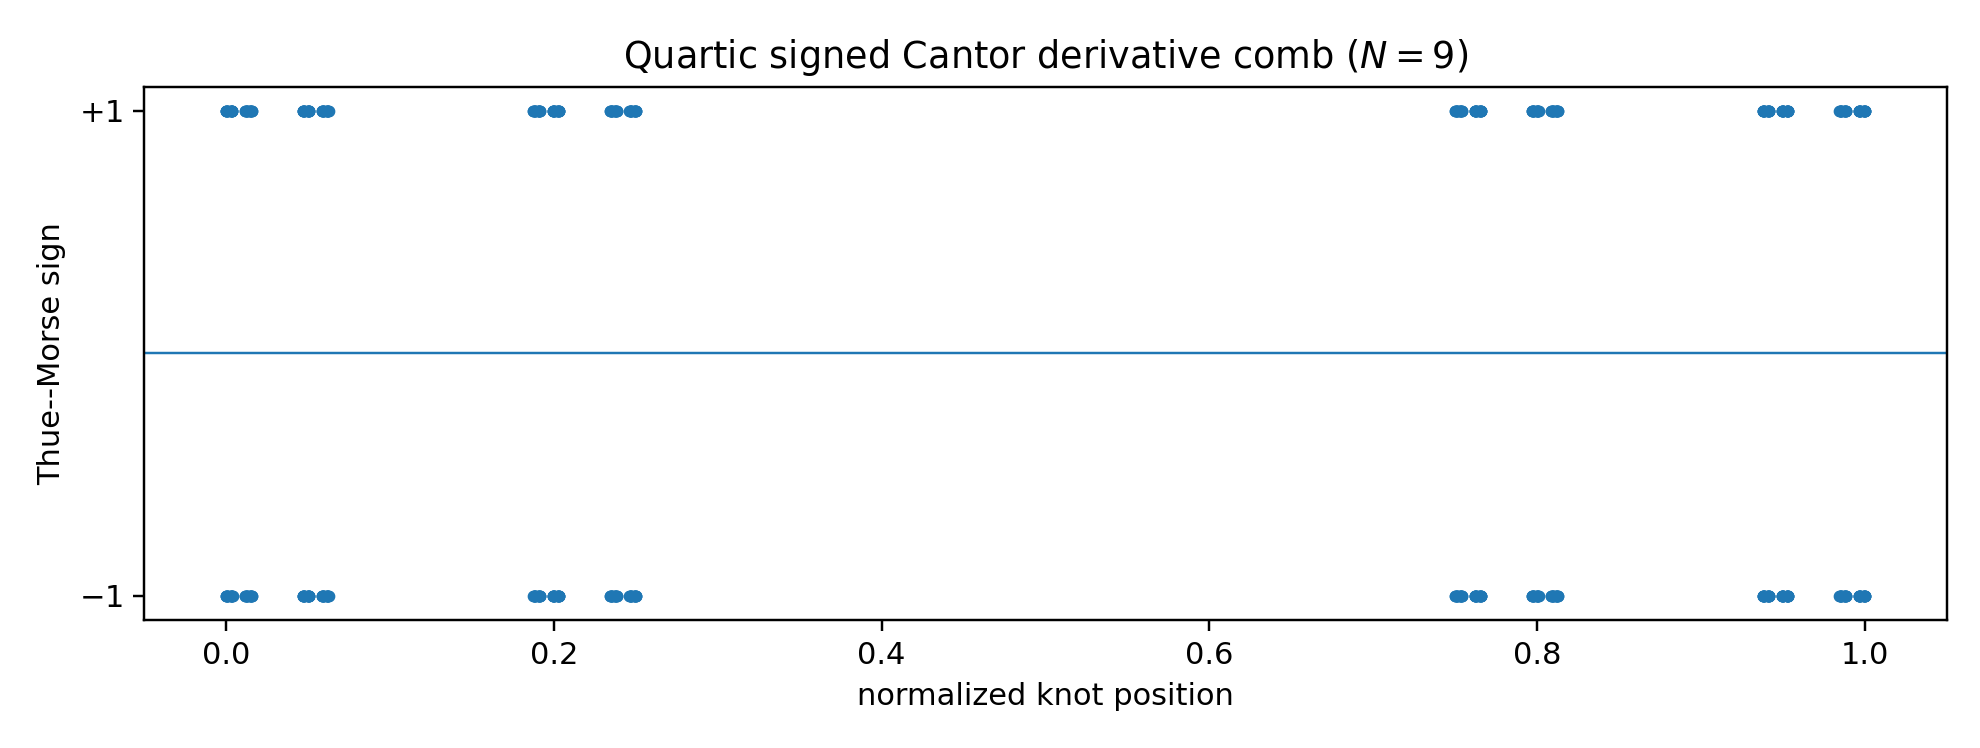
\includegraphics[width=\textwidth]{assets/Signed_Reciprocal_q_Fabius_Frontiers/quartic_cantor_comb.png}
\end{minipage}
\caption{Signed derivative combs at level $N=9$ (ordinate: Thue--Morse
sign).  Left, $q=1/2$: a full dyadic grid.  Right, $q=1/4$: base-four digits
$\{0,1\}$ already displaying the dimension-$1/2$ Cantor geometry of
\eqref{p7:eq:quartic-cantor}.}
\label{p7:fig:combs}
\end{figure}

\section{Reciprocal \texorpdfstring{$q$}{q}-Lagrange rows}
\label{p7:sec:lagrange}

For evaluation at zero from geometric nodes $1,q,\ldots,q^n$, the Lagrange
weights have the closed form
$\lambda^{(q)}_{n,k}=(-1)^{n-k}q^{\binom{n-k+1}2}\qbinom nkq/(q;q)_n$, and
digit --- here node --- reversal gives the exact row reversal (sixteenth
wave)
\begin{equation}\label{p7:eq:lagrange-reversal}
 \boxed{\ \lambda^{(q)}_{n,k}=\lambda^{(q^{-1})}_{n,n-k}:\ }
\end{equation}
the rows for $q=2,-2,4,-4$ are exact reversals of the rows for
$\tfrac12,-\tfrac12,\tfrac14,-\tfrac14$ (the geometric node list for
$q^{-1}$, read backwards and rescaled by $q^n$, is the node list for $q$, and
weights for evaluation at zero are scaling-invariant).  For example, at
$n=5$, $q=\tfrac12$ the exact row is
$\bigl(-\tfrac1{9765},\tfrac2{315},-\tfrac8{63},\tfrac{64}{63},
-\tfrac{1024}{315},\tfrac{32768}{9765}\bigr)$, and the $q=2$ row is its
reversal.  This is the interpolation-theoretic face of the same reciprocity
that inverts the germ and dilates the comb, and it connects directly to the
geometric-Lagrange and $q$-Richardson machinery of Parts~I--II.
\section{Exact inverse-geometric endpoint lattices}
\label{p7:sec:endpoints}

\subsection{The stop-loss simplex formula}

\begin{theorem}[Stop-loss endpoint formula; seventeenth wave]
\label{p7:thm:stop-loss}
Let $0<q<1$, $n\ge1$, and $0\le c\le(1-q)/q$.  Then
\begin{equation}\label{p7:eq:stop-loss}
 \boxed{\ G_q(q^nc)=
 \frac{q^{\,n(n+1)/2}}{(1-q)^n\,n!}\,
 \E\,\pospart{c-Y_q}^{\,n}.\ }
\end{equation}
\end{theorem}

\begin{proof}
Split $Y_q=(1-q)\sum_{j<n}q^jU_j+q^nY_q'$ and condition on $Y_q'=y$.  The
event becomes $\sum_{j<n}(1-q)q^jU_j\le q^n(c-y)$; the threshold is at most
$q^nc\le(1-q)q^{n-1}$, the smallest coordinate width, so the upper cube
constraints are inactive and the conditional probability is the full simplex
volume
$q^{n^2}(c-y)_+^n/\bigl(n!\prod_{j<n}(1-q)q^j\bigr)
=q^{n(n+1)/2}(c-y)_+^n/\bigl((1-q)^nn!\bigr)$.  Average over $y$.
\end{proof}

\subsection{The lattice, its jets, and negative transport}

For $0<q\le\tfrac12$ the value $c=1$ is admissible, and reflection
$1-Y_q\overset d=Y_q$ turns the stop-loss moment into a raw moment.

\begin{corollary}[Inverse-geometric endpoint identity]
\label{p7:cor:inverse-geometric}
For $0<q\le\tfrac12$ and $n\ge0$,
\begin{equation}\label{p7:eq:inverse-geometric}
 \boxed{\ G_q(q^n)=
 \frac{q^{\binom{n+1}2}}{(1-q)^n}\,\frac{m_n(q)}{n!}
 =\frac{q^{\binom{n+1}2}}{(q;q)_n}\,\mathcal P_n(q).\ }
\end{equation}
At $q=\tfrac12$ this is the classical dyadic formula
$F(2^{-n})=2^{-\binom n2}m_n(\tfrac12)/n!$; at $q=\tfrac14$ it gives a new
exact inverse-quartic lattice with first values
\begin{equation}\label{p7:eq:quartic-values}
 G_{1/4}\bigl(\tfrac14\bigr)=\tfrac16,\quad
 G_{1/4}\bigl(\tfrac1{16}\bigr)=\tfrac1{240},\quad
 G_{1/4}\bigl(\tfrac1{64}\bigr)=\tfrac1{51840},\quad
 G_{1/4}\bigl(\tfrac1{256}\bigr)=\tfrac{121}{6768230400}.
\end{equation}
\end{corollary}

\begin{theorem}[Endpoint derivative jets; seventeenth wave]
\label{p7:thm:endpoint-jets}
For $0<q\le\tfrac12$, $n\ge0$, and $0\le r\le n$,
\begin{equation}\label{p7:eq:endpoint-jet}
 \boxed{\ G_q^{(r)}(q^n)=
 (1-q)^{-r}q^{-\binom r2}\,G_q\bigl(q^{\,n-r}\bigr)
 =\frac{q^{\binom{n-r+1}2-\binom r2}}{(1-q)^n}\,
 \frac{m_{n-r}(q)}{(n-r)!}.\ }
\end{equation}
\end{theorem}

\begin{proof}
Conditioning on the first digit gives
$G_q'(x)=\tfrac1{1-q}\bigl[G_q(x/q)-G_q((x-1+q)/q)\bigr]$; on the low
interval $0\le x\le1-q$ the second term vanishes, so
$G_q'(x)=(1-q)^{-1}G_q(x/q)$ --- the CDF face of the edge pantograph equation
\eqref{p6:eq:edge-pantograph}.  Iterating $r$ times multiplies by
$(1-q)^{-r}q^{-(0+1+\cdots+(r-1))}$ and dilates the argument to $x/q^r$; at
$x=q^n$ every intermediate argument stays in the low interval because
$q\le\tfrac12$ (at $q=\tfrac12$, by flat matching of the two smooth
branches).
\end{proof}

In particular
$g_q(q^n)=q^{\,n(n-1)/2}(1-q)^{-n}m_{n-1}(q)/(n-1)!$, and at $r=n$ the jet
collapses to the elementary value $(1-q)^{-n}q^{-\binom n2}$.

\begin{figure}[H]
\centering
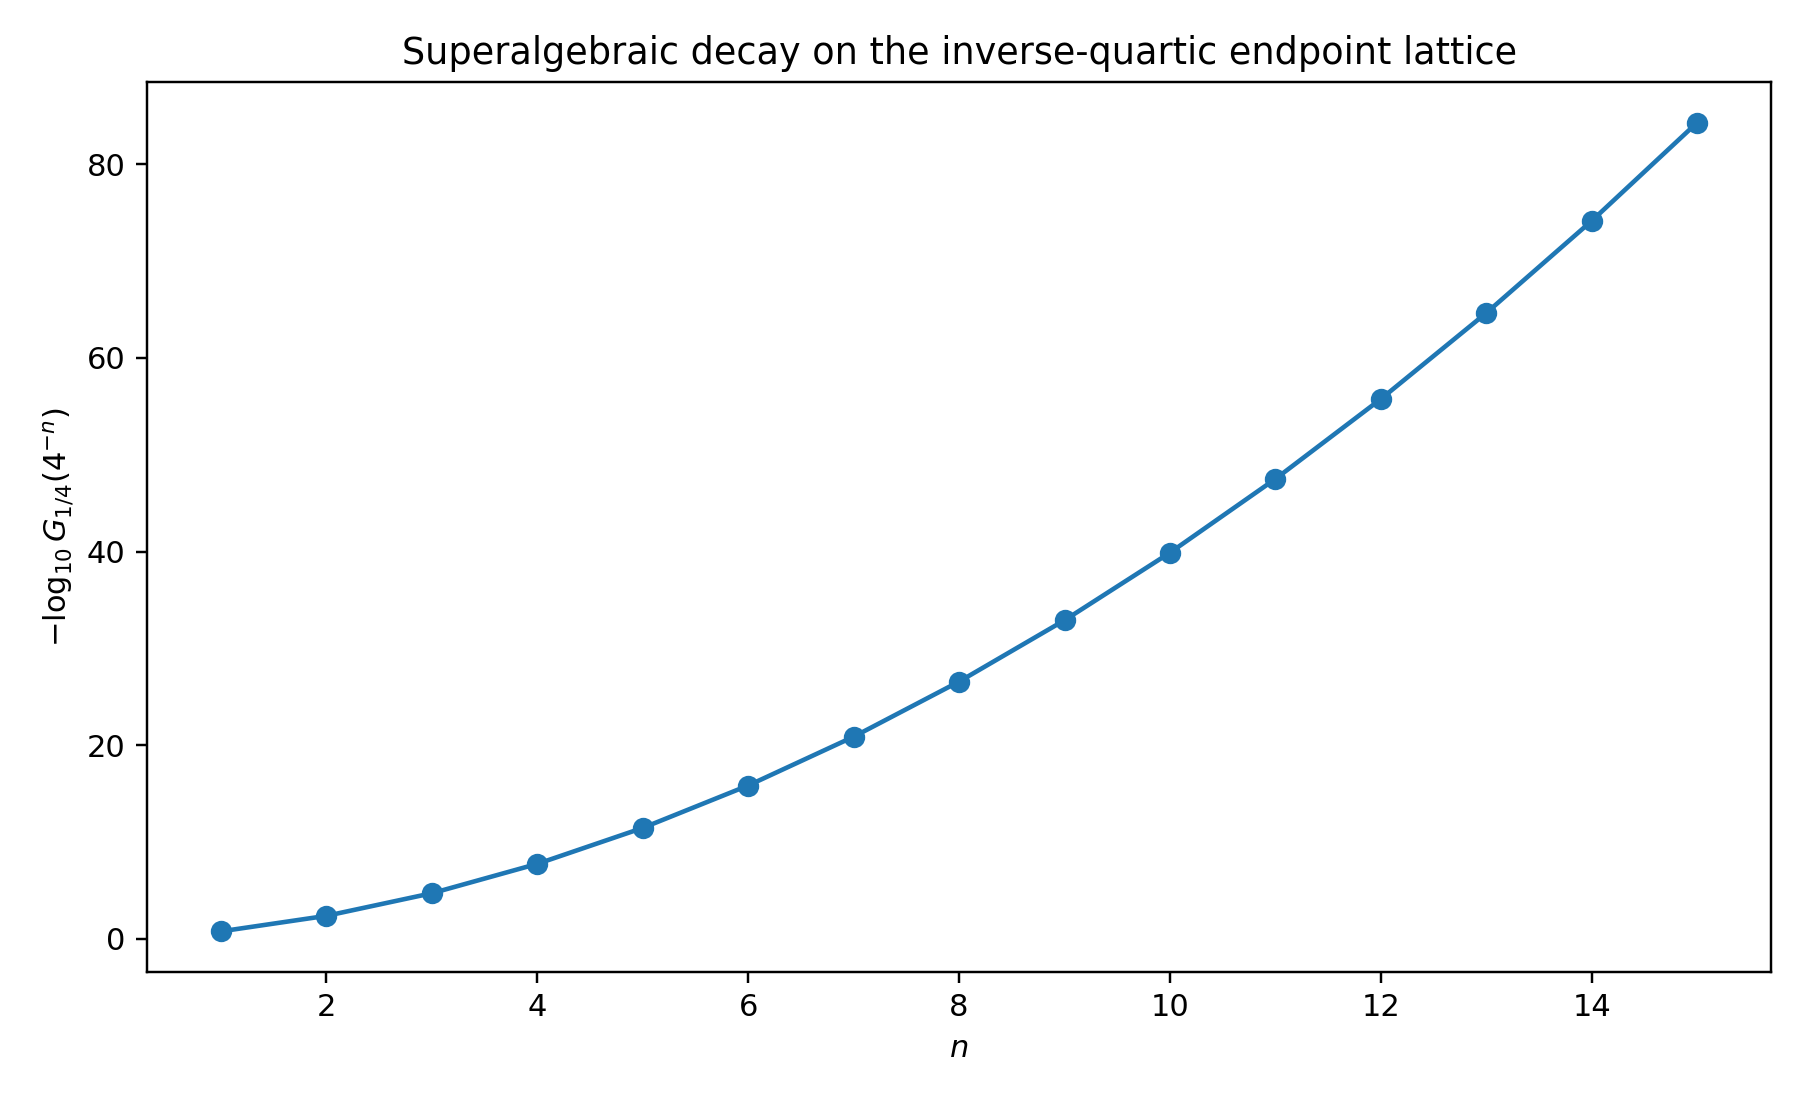
\includegraphics[width=0.78\textwidth]{assets/Signed_Reciprocal_q_Fabius_Frontiers/quartic_endpoint_decay.png}
\caption{Exact inverse-quartic lattice values
\eqref{p7:eq:quartic-values} on a logarithmic ordinate.  The quadratic growth
of $-\log G_{1/4}(4^{-n})$ is the discrete shadow of the two-term endpoint
law of \cref{p7:thm:two-term}.}
\label{p7:fig:quartic-endpoint}
\end{figure}  By the affine
transport \eqref{p7:eq:cdf-transport}, the negative laws inherit the whole
lattice at the shifted nodes $\lambda_aa^n-\beta_a$ (accumulating at the left
endpoint $-\beta_a$), with jets scaled by $\lambda_a^{-r}$; there is no
independent negative-parameter endpoint problem.  Successive lattice ratios
obey
$G_q(q^{n+1})/G_q(q^n)\sim q^{\,n+1}/\bigl((1-q)(n+1)\bigr)$ --- faster than
any geometric rate, the first visible sign of log-squared decay.

\section{Endpoint asymptotics and the general-\texorpdfstring{$q$}{q} Lambert program}
\label{p7:sec:endpoint-asymptotics}

\subsection{A uniform two-term law and its inversion}

\begin{theorem}[Uniform two-term endpoint asymptotic; seventeenth wave]
\label{p7:thm:two-term}
Fix $0<q\le\tfrac12$ and put $L=\log(1/q)$, $\ell=\log(1/x)$.  Then, as
$x\downarrow0$,
\begin{equation}\label{p7:eq:two-term}
 \boxed{\ \log G_q(x)=
 -\frac{\ell^2}{2L}-\frac{\ell\log\ell}{L}+\bigO_q(\ell).\ }
\end{equation}
\end{theorem}

\begin{proof}
At lattice points, \eqref{p7:eq:inverse-geometric} gives
$\log G_q(q^n)=-\tfrac L2n(n+1)-n\log(1-q)-\log n!+\log m_n(q)$.  Reflection
gives the crude bounds $2^{-(n+1)}\le m_n(q)\le1$, so
$\log m_n=\bigO(n)$; Stirling and $n=\ell/L$ give the display, and monotone
bracketing between consecutive lattice points extends it to all $x$.
\end{proof}

\begin{corollary}[Inverse endpoint asymptotic]
\label{p7:cor:inverse-asymptotic}
For fixed $0<q\le\tfrac12$, as $y\downarrow0$,
\begin{equation}\label{p7:eq:inverse-asymptotic}
 \log\frac1{G_q^{-1}(y)}
 =\sqrt{2L\log(1/y)}-\tfrac12\log\log(1/y)+\bigO_q(1).
\end{equation}
\end{corollary}

The dyadic and quartic cases read
$\log F(x)=-\tfrac{\log^2(1/x)}{2\log2}-\tfrac{\log(1/x)\log\log(1/x)}{\log2}
+\bigO(\log(1/x))$ and
$\log G_{1/4}(x)=-\tfrac{\log^2(1/x)}{4\log2}
-\tfrac{\log(1/x)\log\log(1/x)}{2\log2}+\bigO(\log(1/x))$: the quartic law is
less flat at a common $x$ because its scale ladder descends faster.  These
are deliberately weaker but uniform statements; the all-orders periodically
corrected dyadic expansion lives in the inverse-endpoint volume of the
corpus.

\subsection{The periodic cocycle is now exact}

The sixteenth wave formulated the Laplace-side structure as a conjecture: in
the additive coordinate $y=\log((1-r)s)$, $\lambda=\log(1/r)$, the function
$G_r^{\mathrm{coc}}(y)=\log\E\,\e^{-sY_r}$ satisfies the cocycle equation
$G^{\mathrm{coc}}_r(y)-G^{\mathrm{coc}}_r(y-\lambda)
=\log\bigl((1-\e^{-\e^y})/\e^y\bigr)$, and the conjecture asked for the
normal form
$-y^2/(2\lambda)-y/2+C_r+P_r(y/\lambda)+\smallo(1)$ with a real-analytic
one-periodic $P_r$ whose Fourier coefficients come from a Mellin transform.

\begin{theorem}[Resolution by the atomic decomposition]
\label{p7:thm:cocycle-resolved}
The conjectured normal form holds exactly, with an explicit exponentially
small remainder and explicit Fourier coefficients.  Namely, with
$u=(1-r)s$ and $a=1/r$,
\begin{equation}\label{p7:eq:cocycle-exact}
 \log\E\,\e^{-sY_r}
 =\varkappa(u)+\Lambda_{a}(u)
 =-\frac{(\log u)^2}{2\lambda}-\frac{\log u}{2}
 +\Bigl[\varkappa(u)+\log u+P_{a}\bigl(\log_{a}u\bigr)\Bigr]
 +E_{a}(u),
\end{equation}
where $\varkappa,\Lambda_a,P_a,E_a$ are the objects of
\cref{p6:thm:general-periodic}: $P_{a}$ is one-periodic and real analytic
with Fourier modes $-\Gamma(-\chi_k)\zeta(1-\chi_k)/\lambda$,
$\chi_k=2\pi\ii k/\lambda$ (\cref{p6:thm:general-fourier-modes}), the bracket
tends to $P_a(\log_au)$ up to $\bigO(\e^{-u})$ since
$\varkappa(u)=-\log u+\bigO(\e^{-u})$, and
$0\le E_{a}(u)\le\e^{-u}/\bigl((1-\e^{-u})(1-\e^{-(a-1)u})\bigr)$.
\end{theorem}

\begin{proof}
$\E\,\e^{-sY_r}=\prod_{j\ge0}E\bigl(-(1-r)r^js\bigr)$ and
$\log E(-v)=\varkappa(v)$, so the log-Laplace transform is
$\sum_{j\ge0}\varkappa(ur^{j})=\varkappa(u)+\Lambda_{1/r}(u)$.  Apply the
exact decomposition \eqref{p6:eq:general-exact-Laplace} at base $a=1/r$.
\end{proof}

Thus the transform-level half of the general-$q$ endpoint program is closed
--- not only the existence of the periodic correction but its exact
Gamma--zeta Fourier coefficients, uniformly in the base.  What remains open
is the density level, exactly as in Part~VI:

\begin{conjecture}[All-orders general-$q$ endpoint expansion; both waves]
\label{p7:conj:all-orders}
For each $0<q<1$, the density $g_q$, the CDF $G_q$, and the inverse
$G_q^{-1}$ admit, near the left endpoint, complete transseries in inverse
powers of the lower-Lambert coordinate
$w_q(x)=-W_{-1}\bigl(-C_qx\bigr)$ (normalization $C_q$ fixed by the saddle
of \eqref{p7:eq:cocycle-exact}), with coefficient functions real analytic and
one-periodic in $w_q(x)/\log(1/q)$, generated by Bell polynomials in the
derivatives of $P_{1/q}$, reducing at $q=\tfrac12$ to the corpus's dyadic
lower-Lambert hierarchy and matching \cref{p7:thm:two-term} to two orders.
By \cref{p7:cor:transport}, the negative-parameter cases require no separate
analysis.  This is the same open program as Part~VI's refined endpoint
conjecture, now with the quartic case singled out: decimation
\eqref{p7:eq:half-quarter} couples the $q=\tfrac14$ periodic phase to the
dyadic one at two interlaced scales, suggesting that the quartic profile can
be reconstructed from the dyadic profile through a convolution saddle
equation rather than computed from scratch.
\end{conjecture}
\section{Numerical experiments and reproducibility}
\label{p7:sec:numerics}

Both packages are deterministic (no random sampling) and preserved verbatim
under \path{assets/}.

\textbf{Sixteenth wave.}  The package is preserved under
\path{assets/Fabius_Q_Connections_Report/}; its script
\texttt{q\_fabius\_experiments.py} uses exact rational arithmetic for the
finite $q$-binomial, Lagrange, and digit-product identities, 80-digit
arithmetic for the analytic products, and a padded $2^{16}$-point FFT for
density inversion.
Selected residuals: sign conjugacy at $r=\tfrac12$ exact; decimation at
$q=\tfrac12,m=3$ to $6.7\cdot10^{-16}$ (FFT); the sinc--Pochhammer logarithm
at $q=-\tfrac12$ to $3.7\cdot10^{-72}$; Lagrange reciprocal reversal exact
(zero rational mismatches) for all eight orbit values at $n=3,5,7$; the
digit-position product exact at $m=8$; the standardized sign collapse at
$r=\tfrac34$ to $4.8\cdot10^{-16}$; the quarter-base plateau height to
$6.7\cdot10^{-16}$.  Figures: physical densities of the four interior laws
(the negative curves exact affine stretches) and support-normalized profiles.

\textbf{Seventeenth wave.}  The package is preserved under
\path{assets/Signed_Reciprocal_q_Fabius_Frontiers/}; its script
\texttt{numerical\_experiments.py} uses exact \texttt{Fraction} arithmetic
for the moment recurrence (order $\le10$ at all eight values), affine
conjugacy,
reciprocal binomial-convolution inversion, decimation, position-energy
layers ($N\le8$), the $q$-Prouhet transfer ($N\le7$, $\ell\le4$; all
residuals identically zero), the $\mathcal P_n$ recurrence with polynomial
long division for the divisor conjecture ($n\le16$), inverse-geometric
endpoints ($n\le12$ at $q=\tfrac12,\tfrac14$), the Grassmannian/unitary
square ($Q=2,4$, $N\le7$), and the reciprocal Hankel signature through order
nine at $q=\pm2,\pm4$; plus $90$-digit checks of the Mahler, sign,
reciprocal, and decimation product identities (largest residual
$1.3\cdot10^{-40}$, from a deliberately finite $300$-factor truncation under
an argument dilation of five).  Its exact computations were also used as a
theorem-discovery filter: several plausible reciprocity formulas for
$\mathcal P_n$ were rejected before statement --- in this subject,
$q\leftrightarrow1/q$ introduces triangular powers that can make a wrong
formula look valid in low degree.

The exact moment table for the eight orbit values (through $m_6$; e.g.\
$m_4(\tfrac12)=\tfrac{143}{1350}$, $m_6(2)=-\tfrac{16}{59535}$,
$m_4(\tfrac14)=\tfrac{121}{850}$) is in
\path{data/q_orbit_moments.csv} of the seventeenth-wave package, whose
\path{data/} directory also carries the Prouhet, divisibility, endpoint,
finite-geometry, and Hankel tables named in the sections above.

\section{Conjectures, problems, and formalization roadmap}
\label{p7:sec:frontier}

\subsection{Frontier problems}

Beyond \cref{p7:conj:Pn-divisibility,p7:conj:all-orders}, the merged register
is:

\begin{conjecture}[Generic natural boundary; seventeenth wave]
\label{p7:conj:natural-boundary}
For generic fixed $t\ne0$, the unit circle $\abs q=1$ is a natural boundary
for $q\mapsto C_q(t)$, after removal of isolated removable degeneracies: the
cumulant coefficients $(1-q)^{2m}/(1-q^{2m})$ have poles at all roots of
unity, and no single-valued meromorphic continuation should cross a
nontrivial arc.  A proof strategy is to isolate a primitive root-of-unity
singularity in one cumulant order that lower orders cannot cancel; the
partition function $\Zpart_N$ supplies finite approximants with explicit
root-of-unity zero orders.
\end{conjecture}

\begin{problem}[Reciprocal orthogonal polynomials]
Determine the Jacobi coefficients $\beta_n^{(r)}$ of the Laplace dual law
\eqref{p7:eq:Lr} exactly or asymptotically; find the $q$-difference structure
induced by adding one geometric layer; determine the limiting zero
distribution; compare $r=\tfrac12$ and $r=\tfrac14$ through multisection;
and decide membership in a tractable subclass of generalized gamma
convolutions (the signed Laplace differences are not themselves a positive
convolution on $\R_+$).
\end{problem}

\begin{problem}[Arithmetic of $\mathcal P_n$ and of the Appell family]
Find the least $D_n$ with $D_n\mathcal P_n\in\Z[q]$ and compare its prime
valuations with von Staudt--Clausen denominators and the Mersenne/Fermat
factors of $(q;q)_n$ at rational $q$; describe the root geometry of
$\mathcal P_n$ (forced cyclotomic zeros versus limiting curves); develop
multiplication theorems and integrality for $\Br_n^{(r)}$.  Through
decimation, investigate whether the dyadic value arithmetic of Arias de
Reyna and Haugland decomposes into bilinear expressions in quarter-base
values --- negative-parameter value questions reduce affinely and should
never be duplicated.
\end{problem}

\begin{problem}[Two-nome phase diagram and root-of-unity renormalization]
Carry out the $N\to\infty$ saddle analysis of the mixed coefficients of
$\Zpart_N(u,t;\rho,\sigma)$ in the regimes $\abs\rho,\abs\sigma\lessgtr1$ and
on the unit circles, where partial Prouhet cancellation and cyclotomic
resonance occur; construct canonical renormalized limits of the finite laws,
Lagrange rows, and digit products as $q$ approaches a root of unity; and
derive the matrix Mahler system of the four-state pair
$\bigl((-1)^{\wt(n)},\chi(n)\bigr)$ with its Dirichlet series.  Replacing the
lacunary exponent $2^j$ by $b^j$ in $\Xi$ raises the corresponding
joint natural-boundary question on multiplicative-dependence loci.
\end{problem}

\begin{problem}[Quartic Cantor renormalization]
Quantify how the dimension-$\tfrac12$ knot geometry of
\eqref{p7:eq:quartic-cantor} controls finite-level derivative norms and
uniform/Sobolev convergence rates of the quartic box splines; build a
multiresolution basis adapted to base-four digits $\{0,1\}$; and track the
zero divisor $1+\floor{\vtwo(n)/2}$ against the dyadic $1+\vtwo(n)$ through
the convolution \eqref{p7:eq:R-multisection}.
\end{problem}

\subsection{Lean formalization roadmap}

The existing formal development (weighted-uniform series, geometric law,
affine self-similarity, reflection, support, absolute continuity, the Fabius
bridge) supports an incremental plan, merged from both waves.  The low-risk
algebraic tranche: negative affine conjugacy (coordinatewise sign flip and
affine pushforward), geometric multisection (reindex $j=mk+r$), the moment
recurrence and formal uniqueness away from roots of unity, the reciprocity
$M_qM_{1/q}(-\,\cdot)=1$, the position-energy layer over the finite
$q$-binomial core, the two-nome partition function with its multisection, and
the $q$-Prouhet transfer --- finite sums and products throughout, suitable
for the repository's single-worker build.  The endpoint tranche: the
simplex-volume stop-loss formula (upper cube constraints inactive under
\eqref{p7:eq:stop-loss}'s threshold), the lattice identity, the derivative
jets from the CDF pantograph equation, and the two-term asymptotic
(Stirling, crude moment bounds, monotone bracketing) --- far lighter than the
existing all-orders dyadic saddle machinery.  The reciprocal analytic
tranche: the inverse product germ, the Euler rearrangement, the $L^2$ Laplace
series, Hankel positivity and affine transport of determinants, and the
quasi-definite orthogonal recurrence.  Suggested module names:
\texttt{GeometricUniformSign}, \texttt{GeometricUniformMultisection},
\texttt{GeometricProuhet}, \texttt{TwoNomePartition},
\texttt{GeometricEndpoint}, \texttt{GeometricEndpointJets},
\texttt{GeometricEndpointAsymptotic}.  The conjectures of this part remain in
frontier quarantine until proved.

\section{Conclusion}

``Other $q$ values'' do not replace $\tfrac12$ by another number in old
formulas; three transformations act on three layers.  Sign change is an
affine map of the outer normalization --- the centered law is blind to it,
the centered finite transform picks up only the parity
$(-1)^{\binom N2}$, and the finite comb translates.  Inversion turns
smoothing into deconvolution, zeros into poles, real moments into
vertical-line moments, Lagrange rows into their reversals, and finite digit
lists into their reversals.  Decimation splits scales into congruence
classes, factoring the Fabius law over the quartic family, the dyadic
Thue--Morse comb over quartic Cantor combs, and every Pochhammer product over
its dissection.  The finite Gaussian nome and the geometric projection scale
are independent coordinates of one binary-cube partition function whose
renormalized maximal Prouhet jet is the $q$-Fabius moment germ, and whose
position-energy layers carry Grassmannian and Hermitian finite geometry.
Each positive contraction owns an exact inverse-geometric endpoint lattice
with all its jets; each negative law inherits everything affinely; each
reciprocal germ is positive on a vertical line.  The transform-level endpoint
structure is now exact in every base through Part~VI's periodic
decomposition; the density-level all-orders Lambert-$W_{-1}$ program, the
$\mathcal P_n$ arithmetic, and the vertical orthogonal polynomials are the
principal open frontiers.

\begin{thebibliography}{99}

\bibitem{p7:arias-definition}
J. Arias de Reyna,
``An infinitely differentiable function with compact support: Definition and
properties,'' \emph{Rev. Real Acad. Ciencias Madrid} 76 (1982), 21--38;
English translation, arXiv:1702.05442, 2017.

\bibitem{p7:arias-arithmetic}
J. Arias de Reyna,
``Arithmetic of the Fabius function,'' arXiv:1702.06487, 2017.

\bibitem{p7:fabius}
J. Fabius,
``A probabilistic example of a nowhere analytic $C^\infty$-function,''
\emph{Zeitschrift f\"ur Wahrscheinlichkeitstheorie und Verwandte Gebiete}
5 (1966), 173--174.

\bibitem{p7:haugland}
J. K. Haugland,
``Evaluating the Fabius function,'' arXiv:1609.07999, 2016.

\bibitem{p7:fu-reiner-stanton-thiem}
A. M. Fu, V. Reiner, D. Stanton, and P. Thiem,
``The negative $q$-binomial,''
\emph{Electronic Journal of Combinatorics} 19 (2012), Paper P36.

\bibitem{p7:mansour-nguyen}
T. Mansour and H. D. Nguyen,
``A $q$-digital binomial theorem,'' arXiv:1506.07945, 2015; see also
H. D. Nguyen, ``A digital binomial theorem,'' arXiv:1412.3181, 2014.

\bibitem{p7:allouche-shallit}
J.-P. Allouche and J. Shallit,
``The ubiquitous Prouhet--Thue--Morse sequence,'' in \emph{Sequences and
Their Applications}, Springer, 1999, 1--16.

\bibitem{p7:toth}
L. T\'oth,
``Linear combinations of Dirichlet series associated with the Thue--Morse
sequence,'' \emph{Integers} 22 (2022), Article 98.

\bibitem{p7:corless}
R. M. Corless, G. H. Gonnet, D. E. G. Hare, D. J. Jeffrey, and D. E. Knuth,
``On the Lambert $W$ function,'' \emph{Advances in Computational
Mathematics} 5 (1996), 329--359.

\bibitem{p7:gasper-rahman}
G. Gasper and M. Rahman,
\emph{Basic Hypergeometric Series}, 2nd ed., Cambridge University Press,
2004; and NIST DLMF, Chapter 17, for $q$-Pochhammer and Gaussian-binomial
conventions.

\end{thebibliography}

\end{document}
